\ifdefined\ebook
\documentclass[a5paper,oneside]{book}
\newcommand{\FigScale}{0.4}
\else
\documentclass[a4paper,oneside]{book} % oneside: do not put blank page after each chapter. a4paper?
\newcommand{\FigScale}{0.666}
\fi

\usepackage{cmap}
\usepackage{fancyhdr}

\ifdefined\RUSSIAN
\usepackage[english,russian]{babel}
\usepackage[T2A]{fontenc}

% if to turn this font on, copy&paste from Adobe Acrobat to clipboard will not work
%\usepackage{paratype}
%\renewcommand*\familydefault{\sfdefault}

% http://www.emerson.emory.edu/services/latex/latex_169.html
% too small!
%\newcommand{\lstlistingsize}{\scriptsize}

\else
\usepackage[english]{babel}
%\usepackage[T2A]{fontenc}
\usepackage[T1]{fontenc}
\usepackage[default]{sourcesanspro}
% too small!
%\newcommand{\lstlistingsize}{\footnotesize}
\fi

\usepackage[utf8]{inputenc} % but not utf8x - glossary package will grizzle
\usepackage{listings}
\usepackage{ulem}
\usepackage{url}
\usepackage{graphicx}
\usepackage{listingsutf8}
\usepackage{makeidx}
\usepackage{cite}
\usepackage[cm]{fullpage}
\usepackage{color}
\usepackage{fancyvrb}
\usepackage{xspace}
\usepackage{float}
\usepackage{tabularx}
\usepackage{framed}
\usepackage{epigraph}
\usepackage{ccicons}
\usepackage[nottoc]{tocbibind}
\usepackage{longtable}
\usepackage{amsmath}
\usepackage[footnote,printonlyused,withpage]{acronym}
\usepackage[table]{xcolor}% http://ctan.org/pkg/xcolor
\usepackage[]{bookmark,hyperref} % must be last
\usepackage{glossaries}
\usepackage{tikz}
%\usepackage{fixltx2e}
\usepackage{bytefield}
\usepackage{MnSymbol}
\usepackage{shorttoc}
\usetikzlibrary{calc,positioning,chains,arrows}
\ifdefined\ebook
\usepackage[margin=0.5in]{geometry}
\fi

\ifdefined\RUSSIAN
\renewcommand\lstlistingname{Листинг}
\renewcommand\lstlistlistingname{Листинг}
\fi

% fancyhdr
\makeatletter
    \let\stdchapter\chapter
    \renewcommand*\chapter{%
    \@ifstar{\starchapter}{\@dblarg\nostarchapter}}
    \newcommand*\starchapter[1]{%
        \stdchapter*{#1}
        \thispagestyle{fancy}
        \markboth{\MakeUppercase{#1}}{}
    }
    \def\nostarchapter[#1]#2{%
        \stdchapter[{#1}]{#2}
        \thispagestyle{fancy}
    }
\makeatother

\newcommand{\footnoteref}[1]{\textsuperscript{\ref{#1}}}

\definecolor{lstbgcolor}{rgb}{0.94,0.94,0.94}
\makeindex

\newcommand*{\TT}[1]{\texttt{#1}}
\newcommand*{\IT}[1]{\textit{#1}}
\newcommand*{\EN}[1]{\iflanguage{english}{#1}{}}
\newcommand*{\RU}[1]{\iflanguage{english}{}{#1}}
\newcommand{\LANG}{\RU{ru}\EN{en}}
\newcommand*{\dittoclosing}{---''---}
\newcommand*{\EMDASH}{\RU{ --- }\EN{---}}

\newcommand{\ttf}{\TT{f()}\xspace}
\newcommand{\ttfone}{\TT{f1()}\xspace}

% http://tex.stackexchange.com/questions/32160/new-line-after-paragraph
\newcommand{\myparagraph}[1]{\paragraph{#1}\mbox{}\\} 

\newcommand{\figname}{\RU{илл}\EN{fig}.\xspace}
\newcommand{\figref}[1]{\figname{}\ref{#1}\xspace}
\newcommand{\listingname}{\RU{листинг}\EN{listing}.\xspace}
\newcommand{\lstref}[1]{\listingname{}\ref{#1}\xspace}
\newcommand{\bitENRU}{\RU{бит}\EN{bit}\xspace}
\newcommand{\bitsENRU}{\RU{бита}\EN{bits}\xspace}
\newcommand{\Sourcecode}{\RU{Исходный код}\EN{Source code}\xspace}
\newcommand{\Seealso}{\RU{См. также}\EN{See also}\xspace}
\newcommand{\MacOSX}{Mac OS X\xspace}

% FIXME TODO non-overlapping color!
% \newcommand{\headercolor}{\cellcolor{blue!25}}
\newcommand{\headercolor}{}

\newcommand{\tableheader}{\headercolor{} \RU{смещение}\EN{offset} & \headercolor{} \RU{описание}\EN{description}}

\newcommand{\IDA}{\ac{IDA}\xspace}

\newcommand{\tracer}{\protect\gls{tracer}\xspace}

\newcommand{\Tchar}{\IT{char}\xspace} 
\newcommand{\Tint}{\IT{int}\xspace}
\newcommand{\Tbool}{\IT{bool}\xspace}
\newcommand{\Tfloat}{\IT{float}\xspace}
\newcommand{\Tdouble}{\IT{double}\xspace}
\newcommand{\Tvoid}{\IT{void}\xspace}
\newcommand{\ITthis}{\IT{this}\xspace}

\newcommand{\Ox}{\TT{/Ox}\xspace}
\newcommand{\Obzero}{\TT{/Ob0}\xspace}
\newcommand{\Othree}{\TT{-O3}\xspace}

\newcommand{\oracle}{Oracle RDBMS\xspace}

\newcommand{\idevices}{iPod/iPhone/iPad\xspace}
\newcommand{\olly}{OllyDbg\xspace}

% common C functions
\newcommand{\printf}{\TT{printf()}\xspace} 
\newcommand{\puts}{\TT{puts()}\xspace} 
\newcommand{\main}{\TT{main()}\xspace} 
\newcommand{\qsort}{\TT{qsort()}\xspace} 
\newcommand{\strlen}{\TT{strlen()}\xspace} 
\newcommand{\scanf}{\TT{scanf()}\xspace} 
\newcommand{\rand}{\TT{rand()}\xspace} 

% x86 instructions
\newcommand{\ADD}{\TT{ADD}\xspace} 
\newcommand{\ANDIns}{\TT{AND}\xspace} 
\newcommand{\CALL}{\TT{CALL}\xspace} 
\newcommand{\CPUID}{\TT{CPUID}\xspace} 
\newcommand{\CMP}{\TT{CMP}\xspace} 
\newcommand{\DEC}{\TT{DEC}\xspace} 
\newcommand{\FADDP}{\TT{FADDP}\xspace} 
\newcommand{\FCOM}{\TT{FCOM}\xspace}
\newcommand{\FCOMP}{\TT{FCOMP}\xspace}
\newcommand{\FCOMI}{\TT{FCOMI}\xspace}
\newcommand{\FCOMIP}{\TT{FCOMIP}\xspace}
\newcommand{\FUCOM}{\TT{FUCOM}\xspace}
\newcommand{\FUCOMI}{\TT{FUCOMI}\xspace}
\newcommand{\FUCOMIP}{\TT{FUCOMIP}\xspace}
\newcommand{\FUCOMPP}{\TT{FUCOMPP}\xspace}
\newcommand{\FDIVR}{\TT{FDIVR}\xspace} 
\newcommand{\FDIV}{\TT{FDIV}\xspace} 
\newcommand{\FLD}{\TT{FLD}\xspace} 
\newcommand{\FMUL}{\TT{FMUL}\xspace} 
\newcommand{\FSTP}{\TT{FSTP}\xspace} 
\newcommand{\FDIVP}{\TT{FDIVP}\xspace}
\newcommand{\IDIV}{\TT{IDIV}\xspace} 
\newcommand{\IMUL}{\TT{IMUL}\xspace} 
\newcommand{\INC}{\TT{INC}\xspace} 
\newcommand{\JAE}{\TT{JAE}\xspace} 
\newcommand{\JA}{\TT{JA}\xspace} 
\newcommand{\JBE}{\TT{JBE}\xspace} 
\newcommand{\JB}{\TT{JBE}\xspace} 
\newcommand{\JE}{\TT{JE}\xspace} 
\newcommand{\JGE}{\TT{JGE}\xspace} 
\newcommand{\JG}{\TT{JG}\xspace} 
\newcommand{\JLE}{\TT{JLE}\xspace} 
\newcommand{\JL}{\TT{JL}\xspace} 
\newcommand{\JMP}{\TT{JMP}\xspace} 
\newcommand{\JNE}{\TT{JNE}\xspace} 
\newcommand{\JNZ}{\TT{JNZ}\xspace} 
\newcommand{\JNA}{\TT{JNA}\xspace} 
\newcommand{\JNAE}{\TT{JNAE}\xspace} 
\newcommand{\JNB}{\TT{JNB}\xspace} 
\newcommand{\JNBE}{\TT{JNBE}\xspace} 
\newcommand{\JZ}{\TT{JZ}\xspace} 
\newcommand{\JP}{\TT{JP}\xspace} 
\newcommand{\Jcc}{\TT{Jcc}\xspace} 
\newcommand{\SETcc}{\TT{SETcc}\xspace} 
\newcommand{\LEA}{\TT{LEA}\xspace} 
\newcommand{\LOOP}{\TT{LOOP}\xspace}
\newcommand{\MOVSX}{\TT{MOVSX}\xspace} 
\newcommand{\MOVZX}{\TT{MOVZX}\xspace} 
\newcommand{\MOV}{\TT{MOV}\xspace} 
\newcommand{\NOP}{\TT{NOP}\xspace} 
\newcommand{\POP}{\TT{POP}\xspace} 
\newcommand{\PUSH}{\TT{PUSH}\xspace} 
\newcommand{\NOT}{\TT{NOT}\xspace} 
\newcommand{\RET}{\TT{RET}\xspace} 
\newcommand{\RETN}{\TT{RETN}\xspace} 
\newcommand{\SETNZ}{\TT{SETNZ}\xspace} 
\newcommand{\SETBE}{\TT{SETBE}\xspace} 
\newcommand{\SETNBE}{\TT{SETNBE}\xspace} 
\newcommand{\SUB}{\TT{SUB}\xspace} 
\newcommand{\TEST}{\TT{TEST}\xspace} 
\newcommand{\FNSTSW}{\TT{FNSTSW}\xspace}
\newcommand{\SAHF}{\TT{SAHF}\xspace}
\newcommand{\XOR}{\TT{XOR}\xspace} 
\newcommand{\OR}{\TT{OR}\xspace} 
\newcommand{\SHL}{\TT{SHL}\xspace} 
\newcommand{\SHR}{\TT{SHR}\xspace} 
\newcommand{\LEAVE}{\TT{LEAVE}\xspace} 
\newcommand{\MOVDQA}{\TT{MOVDQA}\xspace} 
\newcommand{\MOVDQU}{\TT{MOVDQU}\xspace} 
\newcommand{\PADDD}{\TT{PADDD}\xspace} 
\newcommand{\PCMPEQB}{\TT{PCMPEQB}\xspace} 

% x86 flags

\newcommand{\ZF}{\TT{ZF}\xspace} 
\newcommand{\CF}{\TT{CF}\xspace} 
\newcommand{\PF}{\TT{PF}\xspace} 

% x86 registers

\newcommand{\AL}{\TT{AL}\xspace} 
\newcommand{\AH}{\TT{AH}\xspace} 
\newcommand{\AX}{\TT{AX}\xspace} 
\newcommand{\EAX}{\TT{EAX}\xspace} 
\newcommand{\EBX}{\TT{EBX}\xspace} 
\newcommand{\ECX}{\TT{ECX}\xspace} 
\newcommand{\EDX}{\TT{EDX}\xspace} 
\newcommand{\DL}{\TT{DL}\xspace} 
\newcommand{\ESI}{\TT{ESI}\xspace} 
\newcommand{\EDI}{\TT{EDI}\xspace} 
\newcommand{\EBP}{\TT{EBP}\xspace} 
\newcommand{\ESP}{\TT{ESP}\xspace} 
\newcommand{\RSP}{\TT{RSP}\xspace} 
\newcommand{\EIP}{\TT{EIP}\xspace} 
\newcommand{\RIP}{\TT{RIP}\xspace} 
\newcommand{\RAX}{\TT{RAX}\xspace} 
\newcommand{\RBX}{\TT{RBX}\xspace} 
\newcommand{\RCX}{\TT{RCX}\xspace} 
\newcommand{\RDX}{\TT{RDX}\xspace} 
\newcommand{\RBP}{\TT{RBP}\xspace} 
\newcommand{\RSI}{\TT{RSI}\xspace} 
\newcommand{\RDI}{\TT{RDI}\xspace} 
\newcommand*{\ST}[1]{\TT{ST(#1)}\xspace}
\newcommand*{\XMM}[1]{\TT{XMM#1}\xspace}

% ARM
\newcommand*{\Reg}[1]{\TT{R#1}\xspace}
\newcommand*{\RegX}[1]{\TT{X#1}\xspace}
\newcommand*{\RegW}[1]{\TT{W#1}\xspace}
\newcommand*{\RegD}[1]{\TT{D#1}\xspace}
\newcommand{\ADREQ}{\TT{ADREQ}\xspace}
\newcommand{\ADRNE}{\TT{ADRNE}\xspace}
\newcommand{\BEQ}{\TT{BEQ}\xspace}

% instructions descriptions
\newcommand{\ASRdesc}{\RU{арифметический сдвиг вправо}\EN{arithmetic shift right}}

% x86 registers tables
% TODO: non-overlapping color!
\newcommand{\RegHeader}{
\RU{
 7 \textsuperscript{(номер байта)} &
 6 &
 5 &
 4 &
 3 &
 2 &
 1 &
 0 }
\EN{
 7th \textsuperscript{(byte number)} &
 6th &
 5th &
 4th &
 3rd &
 2nd &
 1st &
 0th}
}

% FIXME навести порядок тут...
\newcommand{\RegTableThree}[5]{
\begin{center}
\begin{tabular}{ | l | l | l | l | l | l | l | l | l |}
\hline
\RegHeader \\
\hline
\multicolumn{8}{ | c | }{#1} \\
\hline
\multicolumn{4}{ | c | }{} & \multicolumn{4}{ c | }{#2} \\
\hline
\multicolumn{6}{ | c | }{} & \multicolumn{2}{ c | }{#3} \\
\hline
\multicolumn{6}{ | c | }{} & #4 & #5 \\
\hline
\end{tabular}
\end{center}
}

\newcommand{\RegTableOne}[5]{\RegTableThree{#1\textsuperscript{x64}}{#2}{#3}{#4}{#5}}

\newcommand{\RegTableTwo}[4]{
\begin{center}
\begin{tabular}{ | l | l | l | l | l | l | l | l | l |}
\hline
\RegHeader \\
\hline
\multicolumn{8}{ | c | }{#1\textsuperscript{x64}} \\
\hline
\multicolumn{4}{ | c | }{} & \multicolumn{4}{ c | }{#2} \\
\hline
\multicolumn{6}{ | c | }{} & \multicolumn{2}{ c | }{#3} \\
\hline
\multicolumn{7}{ | c | }{} & #4\textsuperscript{x64} \\
\hline
\end{tabular}
\end{center}
}

\newcommand{\RegTableFour}[4]{
\begin{center}
\begin{tabular}{ | l | l | l | l | l | l | l | l | l |}
\hline
\RegHeader \\
\hline
\multicolumn{8}{ | c | }{#1} \\
\hline
\multicolumn{4}{ | c | }{} & \multicolumn{4}{ c | }{#2} \\
\hline
\multicolumn{6}{ | c | }{} & \multicolumn{2}{ c | }{#3} \\
\hline
\multicolumn{7}{ | c | }{} & #4 \\
\hline
\end{tabular}
\end{center}
}


\newglossaryentry{tail call}
{
  name=\RU{хвостовая рекурсия}\EN{tail call},
  description={\RU{Это когда компилятор или интерпретатор превращает рекурсию 
  (с которой возможно это проделать, т.е., \IT{хвостовую}) в итерацию для эффективности}
  \EN{It is when compiler (or interpreter) transforms recursion (with which it is possible: \IT{tail recursion}) 
  into iteration for efficiency}: \url{http://en.wikipedia.org/wiki/Tail_call}}
}

\newglossaryentry{endianness}
{
  name=endianness,
  description={\RU{Порядок байт}\EN{Byte order}: \ref{sec:endianness}}
}

\newglossaryentry{caller}
{
  name=caller,
  description={\RU{Ф-ция вызывающая другую ф-цию}\EN{A function calling another}}
}

\newglossaryentry{callee}
{
  name=callee,
  description={\RU{Вызываемая ф-ция}\EN{A function being called by another}}
}

\newglossaryentry{debuggee}
{
  name=debuggee,
  description={\RU{Отлаживаемая программа}\EN{A program being debugged}}
}

\newglossaryentry{leaf function}
{
  name=leaf function,
  description={\RU{Ф-ция не вызывающая больше никаких ф-ций}
  \EN{A function which is not calling any other function}}
}

\newglossaryentry{link register}
{
  name=link register,
  description=(RISC) {\RU{Регистр в котором обычно записан адрес возврата.
  Это позволяет вызывать leaf-функции без использования стека, т.е., быстрее.}
  \EN{A register where return address is usually stored.
  This makes calling leaf functions without stack usage, i.e., faster.}}
}

\newglossaryentry{anti-pattern}
{
  name=anti-pattern,
  description={\RU{Нечто широко известное как плохое решение}
  \EN{Generally considered as bad practice}}
}

\newglossaryentry{stack pointer}
{
  name=\RU{указатель стека}\EN{stack pointer},
  description={\RU{Регистр указывающий на место в стеке.}
  \EN{A register pointing to the place in the stack.}}
}

\newglossaryentry{decrement}
{
  name=\RU{декремент}\EN{decrement},
  description={\RU{Уменьшение на $1$}\EN{Decrease by $1$}}
}

\newglossaryentry{increment}
{
  name=\RU{инкремент}\EN{increment},
  description={\RU{Увеличение на $1$}\EN{Increase by $1$}}
}

\newglossaryentry{loop unwinding}
{
  name=loop unwinding,
  description={\RU{Это когда вместо организации цикла на $n$ итераций, компилятор генерирует $n$ копий тела
  цикла, для экономии на инструкциях, обеспечивающих сам цикл}
  \EN{It is when a compiler instead of generation loop code of $n$ iteration, generates just $n$ copies of the
  loop body, in order to get rid of loop maintenance instructions}}
}

\newglossaryentry{register allocator}
{
  name=register allocator,
  description={\RU{Ф-ция компилятора распределяющая локальные переменные по регистрам процессора}
  \EN{Compiler's function assigning local variables to CPU registers}}
}

\newglossaryentry{quotient}
{
  name=\RU{частное}\EN{quotient},
  description={\RU{Результат деления}\EN{Division result}}
}

\newglossaryentry{product}
{
  name=\RU{произведение}\EN{product},
  description={\RU{Результат умножения}\EN{Multiplication result}}
}

\newglossaryentry{NOP}
{
  name=NOP,
  description={``no operation'', \RU{холостая инструкция}\EN{idle instruction}}
}

\newglossaryentry{POKE}
{
  name=POKE,
  description={\RU{Инструкция языка BASIC записывающая байт по определенному адресу}
  	\EN{BASIC language instruction writing byte on specific address}}
}

\newglossaryentry{keygenme}
{
  name=keygenme,
  description={\RU{Программа, имитирующая защиту вымышленной программы, для которой нужно сделать 
  генератор ключей/лицензий}\EN{A program which imitates fictional software protection,
  for which one needs to make a keys/licenses generator}}
}

\newglossaryentry{dongle}
{
  name=dongle,
  description={\RU{Небольшое устройство подключаемое к LPT-порту для принтера (в прошлом) или к USB}
  \EN{Dongle is a small piece of hardware connected to LPT printer port (in past) or to USB}.
  \RU{Исполняло функции security token-а, имела память и, иногда,
  секретную (крипто-)хеширующую функцию}
  \EN{Its function was akin to security token, it has some memory and, sometimes,
  secret (crypto-)hashing algorithm}.}
}

\newglossaryentry{thunk function}
{
  name=thunk function,
  description={\RU{Крохотная функция делающая только одно: вызывающая другую функцию.}
  \EN{Tiny function with a single role: call another function.}}
}

\newglossaryentry{user mode}
{
  name=user mode,
  description={\RU{Режим CPU с ограниченными возможностями в котором он исполняет прикладное ПО. ср.}
  \EN{A restricted CPU mode in which it executes all applied software code. cf.} \gls{kernel mode}.}
}

\newglossaryentry{kernel mode}
{
  name=kernel mode,
  description={\RU{Режим CPU с неограниченными возможностями в котором он исполняет ядро OS и драйвера. ср.}
  \EN{A restrictions-free CPU mode in which it executes OS kernel and drivers. cf.} \gls{user mode}.}
}

\newglossaryentry{Windows NT}
{
  name=Windows NT,
  description={Windows NT, 2000, XP, Vista, 7, 8}
}

\newglossaryentry{atomic operation}
{
  name=atomic operation,
  description={
  ``$\alpha{}\tau{}o\mu{}o\varsigma{}$''
  %``atomic''
  \RU{означает ``неделимый'' в греческом языке, так что атомарная операция
  это операция которая гарантированно не будет прервана другими тредами}
  \EN{mean ``indivisible'' in Greek, so atomic operation is what guaranteed not
  to be broke up during operation by other threads}}
}

% to be proofreaded (begin)
\newglossaryentry{NaN}
{
  name=NaN,
  description={
  	\RU{не число: специальные случаи чисел с плавающей запятой, обычно сигнализирующие об ошибках}
	\EN{not a number: special cases of floating point numbers, usually signaling about errors}
  }
}

\newglossaryentry{basic block}
{
  name=basic block,
  description={
  	\RU{группа инструкций не имеющая инструкций переходов,
	а также не имеющая переходов в середину блока извне.
	В IDA он выглядит как просто список инструкций без строк-разрывов}
	\EN{a group of instructions not having jump/branch instructions, and also not having
	jumps inside block from the outside.
	In IDA it looks just like as a list of instructions without breaking empty lines}
  }
}

\newglossaryentry{NEON}
{
  name=NEON,
  description={\ac{AKA} ``Advanced SIMD''\EMDASH\ac{SIMD} \RU{от}\EN{from} ARM}
}

\newglossaryentry{reverse engineering}
{
  name=reverse engineering,
  description={\RU{процесс понимания как устроена некая вещь, иногда, с целью клонирования оной}
  \EN{act of understanding, how the thing works, sometimes, in order to clone it}}
}

\newglossaryentry{compiler intrinsic}
{
  name=compiler intrinsic,
  description={\RU{Специфичная для компилятора ф-ция не являющаяся обычной библиотечной ф-цией.
	Компилятор вместо её вызова генерирует определенный машинный код.
	Нередко, это псевдофункции для определенной инструкции \ac{CPU}. Читайте больше:}
	\EN{A function specific to a compiler which is not usual library function.
	Compiler generate a specific machine code instead of call to it.
	It is often a pseudofunction for specific \ac{CPU} instruction. Read more:} (\ref{sec:compiler_intrinsic})}
}

\newglossaryentry{heap}
{
  name=heap,
  description={\RU{(куча) обычно, большой кусок памяти предоставляемый \ac{OS}, так что прикладное ПО может делить его
  как захочет. malloc()/free() работают с кучей.}
  \EN{usually, a big chunk of memory provided by \ac{OS} so that applications can divide it by themselves as they wish.
  malloc()/free() works with heap.}}
}

\newglossaryentry{name mangling}
{
  name=name mangling,
  description={\RU{применяется как минимум в \Cpp, где компилятору нужно закодировать имя класса,
  метода и типы аргументов в одной
  строке, которая будет внутренним именем ф-ции. читайте также здесь}
  \EN{used at least in \Cpp, where compiler need to encode name of class, method and argument types in the one string,
  which will become internal name of the function. read more here}: \ref{namemangling}}
}

\newglossaryentry{xoring}
{
  name=xoring,
  description={\RU{нередко применяемое в английском языке, означает применение операции 
  \ac{XOR}}
  \EN{often used in English language, meaning applying \ac{XOR} operation}}
}

\newglossaryentry{security cookie}
{
  name=security cookie,
  description={\RU{Случайное значение, разное при каждом исполнении. Читайте больше об этом тут}
  \EN{A random value, different at each execution. Read more about it}: \ref{subsec:BO_protection}}
}

\newglossaryentry{tracer}
{
  name=tracer,
  description={\RU{Моя простейшая утилита для отладки. Читайте больше об этом тут}
  \EN{My own simple debugging tool. Read more about it}: \ref{tracer}}
}

\newglossaryentry{GiB}
{
  name=GiB,
  description={\RU{Гибибайт: $2^{30}$ или 1024 мебибайт или 1073741824 байт}
  \EN{Gibibyte: $2^{30}$ or 1024 mebibytes or 1073741824 bytes}}
}

\newglossaryentry{CP/M}
{
  name=CP/M,
  description={Control Program for Microcomputers: \RU{очень простая дисковая \ac{OS} использовавшаяся перед}
  \EN{a very basic disk \ac{OS} used before} MS-DOS}
}

\newglossaryentry{stack frame}
{
  name=stack frame,
  description={\RU{Часть стека, в которой хранится информация связанная с текущей ф-цией: локальные переменные,
  аргументы ф-ции, \ac{RA}, итд}\EN{Part of stack containing information specific to the current functions:
  local variables, function arguments, \ac{RA}, etc}}
}

\newglossaryentry{jump offset}
{
  name=jump offset,
  description={\RU{Часть опкода JMP или Jcc инструкции, просто прибавляется к адресу следующей инструкции,
  и так вычисляется новый \ac{PC}. Может быть отрицательным.}\EN{a part of JMP or Jcc instruction opcode, 
  it just to be added to the address
  of the next instruction, and thus is how new \ac{PC} is calculated. May be negative as well.}}
}

\newglossaryentry{integral type}
{
  name=\RU{интегральный тип данных}\EN{integral data type},
  description={\RU{обычные числа, но не с плавающей точкой}
  \EN{usual numbers, but not floating point ones}}
}

\newglossaryentry{PDB}
{
  name=PDB,
  description={(Win32) \RU{Файл с отладочной информацией, обычно просто имена ф-ций, 
  но иногда имена аргументов ф-ций и локальных переменных}
  \EN{Debugging information file, usually just function names, but sometimes also function
  arguments and local variables names}}
}

\newglossaryentry{NTAPI}
{
  name=NTAPI,
  description={\RU{\ac{API} доступное только в линии Windows NT. 
  Большей частью не документировано Microsoft-ом.}\EN{\ac{API} available only in Windows NT line. 
  Largely, not documented by Microsoft.}}
}

\newcommand{\URLWPDA}
{\RU
 {
  \href{http://go.yurichev.com/17012}{Wikipedia: Выравнивание данных}
 }
 \EN{
  \href{http://go.yurichev.com/17013}{Wikipedia: Data structure alignment}
 }
}

\newcommand{\OracleTablesName}{oracle tables\xspace}
\newcommand{\oracletables}{\OracleTablesName\footnote{\href{http://go.yurichev.com/17014}{yurichev.com}}\xspace}

\newcommand{\WPMAO}
{\RU
{
    \href{http://go.yurichev.com/17015}{wikipedia: Умножение-сложение}
}
\EN{
    \href{http://go.yurichev.com/17016}{wikipedia: Multiply–accumulate operation}
}
}

\newcommand{\BGREPURL}{\href{http://go.yurichev.com/17017}{GitHub}}
\newcommand{\FNMSDNROTxURL}{\footnote{\href{http://go.yurichev.com/17018}{MSDN}}}

\newcommand{\YurichevIDAIDCScripts}{http://go.yurichev.com/17019}

% for index
\newcommand{\GrepUsage}{\IFRU{Использование grep}{grep usage}}
\newcommand{\SyntacticSugar}{\IFRU{Синтаксический сахар}{Syntactic Sugar}}
\newcommand{\CompilerAnomaly}{\IFRU{Аномалии компиляторов}{Compiler's anomalies}}
\newcommand{\CLanguageElements}{\IFRU{Элементы языка Си}{C language elements}}
\newcommand{\CStandardLibrary}{\IFRU{Стандартная библиотека Си}{C standard library}}
\newcommand{\Flags}{\IFRU{Флаги}{Flags}}
\newcommand{\Registers}{\IFRU{Регистры}{Registers}}
\newcommand{\Stack}{\IFRU{Стек}{Stack}}
\newcommand{\Recursion}{\IFRU{Рекурсия}{Recursion}}
\newcommand{\RAM}{\IFRU{ОЗУ}{RAM}}
\newcommand{\ROM}{\IFRU{ПЗУ}{ROM}}
\newcommand{\Pointers}{\IFRU{Указатели}{Pointers}}

\newcommand{\Task}{\IFRU{Задача}{Task}\xspace}
\newcommand{\CCpp}{\IFRU{Си/Си++}{C/C++}\xspace}
\newcommand{\NonOptimizing}{\IFRU{Неоптимизирующий}{Non-optimizing}\xspace}
\newcommand{\Optimizing}{\IFRU{Оптимизирующий}{Optimizing}\xspace}
\newcommand{\NonOptimizingKeil}{\NonOptimizing Keil\xspace}
\newcommand{\OptimizingKeil}{\Optimizing Keil\xspace}
\newcommand{\NonOptimizingXcode}{\NonOptimizing Xcode (LLVM)\xspace}
\newcommand{\OptimizingXcode}{\Optimizing Xcode (LLVM)\xspace}
\newcommand{\ARMMode}{\IFRU{Режим ARM}{ARM mode}\xspace}
\newcommand{\ThumbMode}{\IFRU{Режим thumb}{thumb mode}\xspace}
\newcommand{\ThumbTwoMode}{\IFRU{Режим thumb-2}{thumb-2 mode}\xspace}

\newcommand{\FNQUOTIENT}{\footnote{\IFRU{результат деления}{result of division}}}
\newcommand{\FNPRODUCT}{\footnote{\IFRU{результат умножения}{result of multiplication}}}
\newcommand{\FNSUM}{\footnote{\IFRU{результат сложения}{result of addition}}}

\newcommand{\DataProcessingInstructionsFootNote}{\IFRU{Эти инструкции также называются}
{These instructions are also called} ``data processing instructions''}

\newcommand{\Instructions}{\IFRU{Инструкции}{Instructions}}

% section names
\newcommand{\ShiftsSectionName}{\IFRU{Сдвиги}{Shifts}}
\newcommand{\SignedNumbersSectionName}{\IFRU{Представление знака в числах}{Signed number representations}}
\newcommand{\HelloWorldSectionName}{Hello, world!}
\newcommand{\SwitchCaseDefaultSectionName}{switch()/case/default}
\newcommand{\PrintfSeveralArgumentsSectionName}{\printf \IFRU{с несколькими агрументами}{with several arguments}}
\newcommand{\DivisionByNineSectionName}{\IFRU{Деление на 9}{Division by 9}}
\newcommand{\WorkingWithFloatAsWithStructSubSubSectionName}{\IFRU
{Работа с типом float как со структурой}{Working with the float type as with a structure}}

\newcommand{\StructurePackingSectionName}{\IFRU{Упаковка полей в структуре}{Fields packing in structure}}

\newcommand{\PICcode}{\IFRU{адресно-независимый код}{position-independent code}}
\newcommand{\CapitalPICcode}{\IFRU{Адресно-независимый код}{Position-independent code}}

% C
\newcommand{\PostIncrement}{\IFRU{Пост-инкремент}{Post-increment}}
\newcommand{\PostDecrement}{\IFRU{Пост-декремент}{Post-decrement}}
\newcommand{\PreIncrement}{\IFRU{Пре-инкремент}{Pre-increment}}
\newcommand{\PreDecrement}{\IFRU{Пре-декремент}{Pre-decrement}}

% other
\newcommand{\IntelSyntax}{\IFRU{Синтаксис Intel}{Intel syntax}}
\newcommand{\ATTSyntax}{\IFRU{Синтаксис AT\&T}{AT\&T syntax}}



\makeglossaries

\newcommand{\TITLE}{\IFRU{Reverse Engineering для начинающих}
{Reverse Engineering for Beginners}}
\newcommand{\AUTHOR}{\IFRU{Денис Юричев}{Dennis Yurichev}}
\newcommand{\EMAIL}{dennis@yurichev.com}

\hypersetup{
    pdftex,
    colorlinks=true,
    allcolors=blue,
    pdfauthor={\AUTHOR},
    pdftitle={\TITLE}
    }

\lstset{
    backgroundcolor=\color{lstbgcolor},
    basicstyle=\ttfamily,
    %basicstyle=\ttfamily\lstlistingsize, 
    breaklines=true,
    prebreak=\raisebox{0ex}[0ex][0ex]{\ensuremath{\rhookswarrow}},
    postbreak=\raisebox{0ex}[0ex][0ex]{\ensuremath{\rcurvearrowse\space}},
    frame=single,
    columns=fullflexible,keepspaces,
}
\RU{\lstset{inputencoding=cp1251}}

\DeclareMathSizes{12}{30}{16}{12}

\begin{document}
%\setlength{\headheight}{15.2pt}
\setlength{\headheight}{20pt}
\pagestyle{fancy}

\VerbatimFootnotes

\frontmatter

\begin{titlepage}
\ifdefined\ebook % FIXME
\else
\begin{center}
\vspace*{\fill}

\Huge Reverse Engineering \RU{для начинающих}\EN{for Beginners}

\bigskip
\bigskip

\begin{figure}[H]
\centering
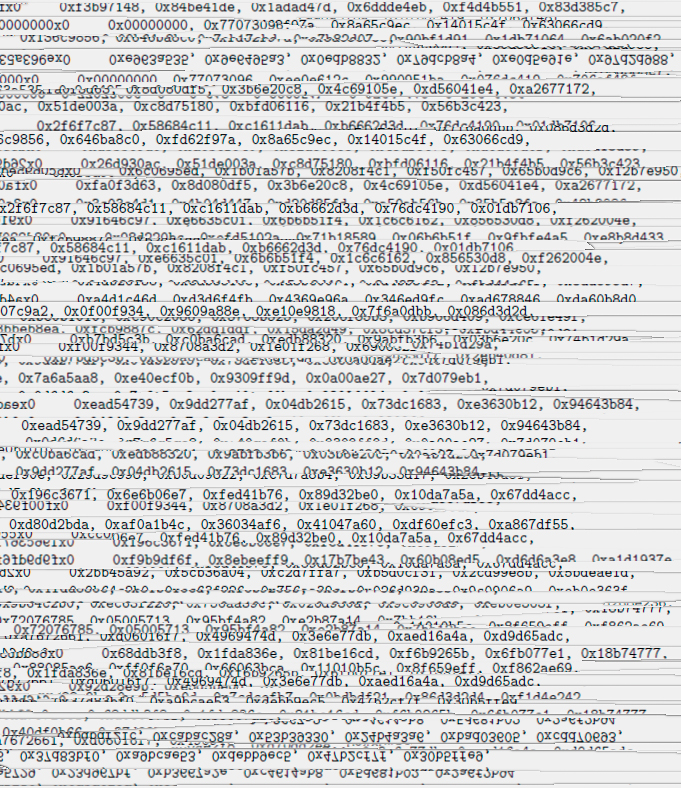
\includegraphics[scale=\FigScale]{cover.jpg}
\end{figure}

\bigskip

\hfill \huge \AUTHOR

\vspace*{\fill}
\end{center}

\newpage
\fi

\begin{center}
\vspace*{\fill}
\LARGE \TITLE

\vspace*{\fill}

\large \AUTHOR

\large \TT{<\EMAIL>}
\vspace*{\fill}
\vfill

\ccbyncnd

\textcopyright 2013-2014, \AUTHOR. 

\IFRU{Это произведение доступно по лицензии Creative Commons «Attribution-NonCommercial-NoDerivs» 
(«Атрибуция — Некоммерческое использование — Без производных произведений») 3.0 Непортированная. 
Чтобы увидеть копию этой лицензии, посетите}
{This work is licensed under the Creative Commons Attribution-NonCommercial-NoDerivs 3.0 Unported License. 
To view a copy of this license, visit} \url{http://creativecommons.org/licenses/by-nc-nd/3.0/}.

\IFRU{Версия этого текста}{Text version} ({\large \today}).

\IFRU{Возможно, более новая версии текста, а также англоязычная версия, также доступна по ссылке}
{There is probably a newer version of this text, and also Russian language version also accessible at} 
\url{http://yurichev.com/RE-book.html}.
\ifdefined\ebook
\IFRU{Версия формата A4 так же доступна по ссылке}
{A4-format version is also available on the page}.
\else
\IFRU{Версия для электронных читалок так же доступна по ссылке}
{E-book reader version is also available on the page}.
\fi

\IFRU{Вы также можете подписаться на мой twitter для получения информации о новых версиях этого текста, 
и т.д: \TT{@yurichev\_ru}\footnote{\url{https://twitter.com/yurichev_ru}}, 
либо подписаться на список рассылки}
{You may also subscribe to my twitter, to get information about updates of this text, etc: 
\TT{@yurichev}\footnote{\url{https://twitter.com/yurichev}}, or to subscribe to mailing list}
\footnote{\url{http://yurichev.com/mailing_lists.html}}.

\end{center}
\end{titlepage}

\begin{center}
\vspace*{\fill}

\Huge\IFRU{Пожалуйста жертвуйте}
{Please donate}!
\normalsize

\bigskip
\bigskip
\bigskip

\Large\IFRU{Я писал эту книгу не менее года, здесь более 600 страниц, и она бесплатная.
Книги такого же уровня стоят от \$20 до \$50.}
{I worked more than year on this book, here are more than 600 pages, and it's free.
Same level books has price tag from \$20 to \$50.}
\normalsize

\bigskip
\bigskip
\bigskip

\IFRU{Больше об этом}{More about it}: \ref{sec:donate}.

\vspace*{\fill}
\vfill
\end{center}


\shorttoc{\IFRU{Краткое оглавление}{Short contents}}{-1} % Only sections
\tableofcontents
\cleardoublepage

\cleardoublepage
\chapter{\IFRU{Введение}{Preface}}

\IFRU
{Здесь (будет) немного моих заметок о reverse engineering на русском языке для начинающих, 
для тех кто хочет научиться понимать создаваемый \CCpp компиляторами код для x86 (коего, 
практически, больше всего остального) и ARM.}
{Here (will be) some of my notes about reverse engineering in English language for 
those beginners who like to learn to understand x86 (which is a most large mass of 
all executable software in the world) and ARM code created by \CCpp compilers.}

\IFRU{У термина ``reverse engineering'' минимум два популярных значения: 1) исследование скомпилированных
программ; 2) сканирование трехмерной модели для последующего копирования. Настоящий сборник заметок
связан с первым значением}
{There are two popular meaning of ``reverse engineering'' term: 1) research into compiled programs;
scan of 3D model in order to make a copy of it. These notes are related to first meaning.}

% \section{\IFRU{Целевая аудитория}{Target audience}}



\mainmatter

% only chapters here!
%FIXME: requires PTBR and ES revision (dbmussi)
\part{\RU{Образцы кода}\EN{Code patterns}\PTBR{Padrões de código}\ES{Patrones de código}}

\RU{\epigraph{Всё познается в сравнении}{Автор неизвестен}}
\EN{\epigraph{Everything is comprehended in comparison}{Author unknown}}
\PTBR{\epigraph{Tudo é relativo}{Autor desconhecido}}
\ES{\epigraph{Todo es relativo}{Autor desconocido}}
% FIXME: english sentence added. (dbmussi) 
% not sure it's correct. (yurichev)
% this is popular Russian proverb and is close to "everything is comprehended in comparison", but the source is lost, however, 
% it's traditionally attributed to all sorts of philosophers..
% I don't know exact analgoue in English language, but OK, let it be so.

\RU{Когда автор этой книги учил Си, а затем \Cpp, он просто писал небольшие фрагменты кода, компилировал и смотрел, что 
получилось на ассемблере. Так было намного проще понять%
\footnote{Честно говоря, он и до сих пор так делаю, когда не понимают, как работает некий код.}.
Он делал это такое количество раз, что связь между кодом на \CCpp и тем, что генерирует компилятор, вбилась в его подсознание достаточно глубоко.
После этого не трудно, глядя на код на ассемблере, сразу в общих чертах понимать, что там было написано на Си. 
Возможно это поможет кому-то ещё.}
\EN{When the author of this book first started learning C and, later, \Cpp, he used to write small pieces of code, compile them, 
and then look at the assembly language output. This made it very easy for him to understand what was going on in the code that he had written.
\footnote{In fact, he still does it when he can't understand what a particular bit of code does.}. 
He did it so many times that the relationship between the \CCpp code and what the compiler produced was imprinted deeply in his mind. 
It's easy to imagine instantly a rough outline of C code's appearance and function. 
Perhaps this technique could be helpful for others.}
\PTBR{Quando o autor deste livro começou a aprender C e, mais tarde, \Cpp, ele costumava escrever pequenos pedaços de código, compilá-los, 
e então olhar a saída em linguagem assembly. Isso tornou muito fácil para ele entender o que estava acontecendo no código que ele tinha escrito.
\footnote{Na verdade, ele ainda faz isso quando não consegue entender o que faz um determinado pedaço de código.}. 
Ele fez isso tantas vezes que o relacionamento entre o código \CCpp code e o que o compilador produzia ficou registrado profundamente em sua mente. 
É fácil imaginar de imediato um esboço da aparência e função do código C. 
Talvez essa técnica poderia ser útil para mais alguém.}
\ES{Cuando el autor de este libro comenzó a aprender C y, más tarde, \Cpp, él solía escribir pequeños trozos de código, compilarlos, 
y luego ver los resultados en lenguaje assembly. Esto lo hizo muy fácil para él entender lo que estaba pasando en el código que había escrito.
\footnote{De hecho, todavia lo hace cuando no puede entender lo que hace una determinada pieza de código.}. 
Él lo hizo tantas veces que la relación entre el código \CCpp y lo que el compilador producido se imprimió profundamente en su mente. 
És fácil imaginar al instante un esbozo de la aparencia y función del código C. 
Quizás esta técnica podría ser útil para otra persona.}

%
%\RU{Здесь много примеров и для x86/x64 и для ARM}\EN{There are a lot of examples for both x86/x64 
%and ARM}.\PTBR{Há uma série de exemplos para ambos x86/x64 e ARM}.\ES{Hay una serie de ejemplos, tanto para x86/x64 y ARM} 
%\RU{Те, кто уже хорошо знаком с одной из архитектур, могут легко пролистывать страницы}
%\EN{Those who already familiar with one of architectures, may freely skim over pages}.
%\PTBR{Aqueles já familiarizados com alguma das arquiteturas, pode ler superficialmente as próximas páginas}.
%\ES{Los que ya están familiarizados con alguna de las arquitecturas, pueden leer superficialmente las páginas siguientes}.

\RU{Иногда здесь используются достаточно древние компиляторы, чтобы получить самый короткий (или простой) фрагмент кода.}%
\EN{Sometimes ancient compilers are used here, in order to get the shortest (or simplest) possible code snippet.}
\PTBR{Em determinadas partes foram usados aqui compiladores muito antigos, para se obter o menor (ou mais simples) snippet possível.}
\ES{En ciertas partes, se han empleado aquí compiladores muy antiguas, con el fin de obtener lo mas corta (o simple) posible snippet.}
\

\ifdefined\IncludeExercises
\section*{\Exercises}

\RU{Когда автор этой книги учил ассемблер, он также часто компилировал короткие функции на Си и затем постепенно 
переписывал их на ассемблер, с целью получить как можно более короткий код.}%
\EN{When the author of this book studied assembly language, he also often compiled small C-functions and then rewrote
them gradually to assembly, trying to make their code as short as possible.}
\PTBR{Quando o autor deste livro estudou a linguagem assembly, ele também frequentemente compilava pequenas funções em C e então as reescrevia gradualmente em assembly, tentando fazer seu código o menor possível.}
\ES{Cuando el autor de este libro estudió la lenguaje assembly, también con frecuencia compilaba pequeñas funciones en C, y reescribia gradualmente en assembly, tratando de hacer el código lo más pequeño posible}
\RU{Наверное, этим не стоит заниматься в наше время на практике (потому что конкурировать с современными
компиляторами в плане эффективности очень трудно), но это очень хороший способ разобраться в ассемблере
лучше.}%
\EN{This probably is not worth doing in real-world scenarios today, 
because it's hard to compete with modern compilers in terms of efficiency. It is, however, a very good way to gain a better understanding of assembly.}
\PTBR{Provavelmente não vale mais à pena fazer isso em cenários reais atualmente, 
porque é difícil competir com os compiladores modernos em termos de eficiência. É, no entanto, uma forma muito boa de obter um melhor entendimento de assembly.}
\ES{Probablemente no vale la pena hacer esto en escenarios reales actualmente, 
porque es dificil competir con los compiladores modernos en términos de eficiencia. Es, sin embargo, una muy buena manera de obtener una mejor compreensión de la assembly}

\RU{Так что вы можете взять любой фрагмент кода на ассемблере в этой книге и постараться сделать его короче.}%
\EN{Feel free, therefore, to take any assembly code from this book and try to make it shorter.}
\PTBR{Sinta-se livre, portanto, para pegar qualquer código assembly deste livro e tentar torná-lo menor.}
\ES{Siéntase libre, por lo tanto, para tomar cualquier código de este libro y tratar de hacerlo más pequeño.}
\RU{Но не забывайте о тестировании своих результатов.}%
\EN{However, don't forget to test what you have written.}
\PTBR{No entanto, não esqueça de testar o que você tiver escrito.}
\ES{Sin embargo, no se olvide de probar lo que has escrito.}
\fi

% rewrote to show that debug\release and optimisations levels are orthogonal concepts.
\section*{\RU{Уровни оптимизации и отладочная информация}\EN{Optimization levels and debug information}\PTBR{Níveis de otimização e informação de depuração}\ES{Níveles de optimización y la información de depuración}}

\RU{Исходный код можно компилировать различными компиляторами с различными уровнями оптимизации.
В типичном компиляторе этих уровней около трёх, где нулевой уровень~--- отключить оптимизацию.
Различают также направления оптимизации кода по размеру и по скорости.}
\EN{Source code can be compiled by different compilers with various optimization levels.
A typical compiler has about three such levels, where level zero means disable optimization.
Optimization can also be targeted towards code size or code speed.}
\PTBR{O código-fonte pode ser compilado por diferentes compiladores com vários níveis de otimização.
Um compilador típico tem cerca de três destes níveis, onde o nível zero significa desativar a otimização.
A otimização também pode ser direcionada para o tamanho do código ou para a velocidade do código.}
\ES{El código fuente puede ser compilado por diferentes compiladores com varios niveles de optimización.
Un compilador típico tiene alredor de tres de esos niveles, donde el nivel cero significa desactivar la optimización.
La optimización también puede dirigirse hacia el tamaño del código o la velocidad de código.}

\RU{Неоптимизирующий компилятор работает быстрее, генерирует более понятный (хотя и более объемный) код.
Оптимизирующий компилятор работает медленнее и старается сгенерировать более быстрый (хотя и не обязательно краткий) код.}
\EN{A non-optimizing compiler is faster and produces more understandable (albeit verbose) code,
whereas an optimizing compiler is slower and tries to produce code that runs faster (but is not necessarily more compact).}
\PTBR{Um compilador sem otimização é mais rápido e produz código mais inteligível (embora maior),
enquanto que um compilador com otimização é mais lento e tenta produzir um código que execute mais rápido (mas não é necessariamente mais compacto).}
\ES{Un compilador sin optimización es más rápido y produce código más inteligible (aunque más grande), 
mientras un compilador con optimización es más lento y trata de producir un código que corre más rápido (pero no necesariamente más compacto).}

\RU{Наряду с уровнями и направлениями оптимизации компилятор может включать в конечный файл отладочную информацию,
производя таким образом код, который легче отлаживать.}
\EN{In addition to optimization levels and direction, a compiler can include in the resulting file some debug information,
thus producing code for easy debugging.}
\PTBR{Além dos níveis e direcionamento da otimização, o compilador pode incluir no arquivo resultante algumas informações de depuração, produzindo assim código para fácil depuração.}
\ES{Además de los niveles y dirección de la otimización, el compilador puede incluir informaciones de depuración en el archivo resultante, produciendo así código para fácil depuración.}

\RU{Одна очень важная черта отладочного кода в том, что он может содержать
связи между каждой строкой в исходном коде и адресом в машинном коде.}
\EN{One of the important features of the ´debug' code is that it might contain links
between each line of the source code and the respective machine code addresses.}
\PTBR{Uma das características importantes do código de ´debug' é que ele pode conter 
ligações entre cada linha do código-fonte e os respectivos endereços de código de máquina.}
\ES{Una de los características importantes del código de ´debug' és que puede contener enlaces entre
cada línea del código fuente y las direcciones de código de máquina respectivos.}
\RU{Оптимизирующие компиляторы обычно генерируют код, где целые строки из исходного кода
могут быть оптимизированы и не присутствовать в итоговом машинном коде.}
\EN{Optimizing compilers, on the other hand, tend to produce output where entire lines of source code
can be optimized away and thus not even be present in the resulting machine code.}
\PTBR{Compiladores com otimização, por outro lado, tendem a produzir uma saída onde linhas inteiras de código-fonte podem ser otimizadas a ponto de serem removidas e portanto não estarem presentes no código de máquina resultante.}
\ES{Compiladores con optimización, por otro lado, tienden a producir una salida donde líneas enteras de código fuente pueden ser optimizados al punto de ser eliminados y por consiguiente no estar presentes en el código de máquina resultante.}

\RU{Практикующий reverse engineer обычно сталкивается с обоими версиями, потому что некоторые разработчики
включают оптимизацию, некоторые другие\EMDASH{}нет. Вот почему мы постараемся поработать с примерами для обоих версий.}
\EN{Reverse engineers can encounter either version, simply because some developers turn on the compiler's optimization flags and others do not. 
Because of this, we'll try to work on examples of both debug and release versions of the code featured in this book, where possible.}
\PTBR{Engenheiros Reversos podem encontrar ambas as versões, simplesmente porque alguns desenvolvedores ativam as flags de otimização do compilador e outros não ativam. 
Por causa disso, nós tentaremos trabalhar em exemplos de ambas as versões de debug e release do código destacado neste livro, onde possível.}
\ES{Ingenieros Inversos pueden encontrar ambas versiones, simplesmente porque alguns desarrolladores activan los flags de optimización del compilador, y otros no activan. 
Debido a esto, vamos a tratar de trabajar con ejemplos de ambas versiones de debug y release del código resaltado en este libro, cuando sea posible.}

\chapter{\RU{Краткое введение в CPU}\EN{A short introduction to the CPU}\PTBR{Uma breve introdução à CPU}\ES{Una breve introducción a la CPU}}

\EN{The}\PTBR{A}\ES{La} \ac{CPU} \RU{это устройство исполняющее все программы}\EN{is the device that executes the machine code a program consists of}\PTBR{é o dispositivo que executa o código de máquina que consiste num programa}\ES{es el dispositivo que ejecuta el código de máquina que constituye un programa}.

\textbf{\RU{Немного терминологии}\EN{A short glossary}\PTBR{Um pequeno glossário}\ES{Un breve glosario}:}

\begin{description}
\item[\RU{Инструкция}\EN{Instruction}\PTBR{Instrução}\ES{Instrucción}]: \RU{примитивная команда}\EN{A primitive}\PTBR{Um primitivo}\ES{Una primitiva}
	\ac{CPU}\RU{.} \EN{command.}\PTBR{comando.}\ES{comando.}
\RU{Простейшие примеры: перемещение между регистрами, работа с памятью, примитивные арифметические операции}%
\EN{The simplest examples include: moving data between registers, working with memory, primitive arithmetic operations}
\PTBR{Os exemplos mais simples incluem: mover dados entre registradores, trabalhar com a memória, operações aritiméticas primitivas}
\ES{Los ejemplos más simples incluyen: mover datos entre registros, trabajar con la memoria, operaciones aritméticas primitivas}.
\RU{Как правило, каждый}\EN{As a rule, each}\PTBR{Como regra geral, cada}\ES{Como regla general, cada} \ac{CPU} \RU{имеет свой набор инструкций}\EN{has its own instruction set architecture}\PTBR{tem seu próprio conjunto de instruções}\ES{tiene su proprio conjunto de instrucciones} 
(\ac{ISA}).

\item[\RU{Машинный код}\EN{Machine code}]: \RU{код понимаемый}\EN{Code that the}\PTBR{Código que a}\ES{Código que la} \ac{CPU}\EN{ directly processes}\PTBR{ processa diretamente}\ES{ procesa directamente}. 
\RU{Каждая инструкция обычно кодируется несколькими байтами}\EN{Each instruction is usually encoded by several bytes}\PTBR{Cada instrução é normalmente codificada em vários bytes}\ES{Cada instrucción generalmente se codifica por vários bytes}.

\item[\RU{Язык ассемблера}\EN{Assembly language}\PTBR{Linguagem assembly}\ES{Lenguaje assembly}]: 
\RU{машинный код плюс некоторые расширения, призванные облегчить труд программиста: макросы, имена, \etc.}
\EN{Mnemonic code and some extensions like macros that are intended to make a programmer's life easier.}
\PTBR{Código mnemônico e algumas extensões como macros que têm a finalidade de facilitar a vida do programamdor.}
\ES{Código mnemónico y algunas extensiones como macros que destinados a hacer la vida del programador más fácil.}

\item[\RU{Регистр CPU}\EN{CPU register}\PTBR{Registradores da CPU}\ES{Registros de la CPU}]: 
\RU{Каждый}\EN{Each}\PTBR{Cada}\ES{Cada} \ac{CPU} \RU{имеет некоторый фиксированный набор регистров общего назначения}\EN{has a fixed set of general purpose registers}\PTBR{tem um conjunto fixo de registradores de propósito geral}\ES{tiene un conjunto fijo de registros de propósito general} (\ac{GPR}).
$\approx 8$ \InENRU x86, $\approx 16$ \InENRU x86-64, $\approx 16$ \InENRU ARM.
\RU{Проще всего понимать регистр как временную переменную без типа}%
\EN{The easiest way to understand a register is to think of it as an untyped temporary variable}
\PTBR{A forma mais fácil de entender um registrador é pensar nele como uma variável temporária não tipada}
\ES{La forma más fácil de entender un registro es pensar en ello como una variable temporal sin tipo}.
\RU{Можно представить, что вы пишете на \ac{PL} высокого уровня и у вас только 8 переменных шириной 32 (или 64) бита}%
\EN{Imagine if you were working with a high-level \ac{PL} and could only use eight 32-bit (or 64-bit) variables}
\PTBR{Imagine que você estivesse trabalhando com uma \ac{PL} de alto nível e pudesse usar apenas oito variáveis de 32-bit (ou de 64-bit)}
\ES{Imagine si estuviera trabajando con una \ac{PL} de alto nivel y sólo podría utilizar ocho variables de 32-bit (o de 64-bit)}.
\RU{Можно сделать очень много используя только их}\EN{Yet a lot can be done using just these}\PTBR{No entanto, muito ainda pode ser feito usando apenas eles}\ES{Sin embargo mucho se puede hacer usando sólo estos}!
\end{description}

\RU{Откуда взялась разница между машинным кодом и \ac{PL} высокого уровня?
Ответ в том, что люди и \ac{CPU}-ы отличаются друг от друга\EMDASH{}}
\EN{One might wonder why there needs to be a difference between machine code and a \ac{PL}.
The answer lies in the fact that humans and \ac{CPU}s are not alike\EMDASH{}}
\PTBR{Alguém poderia perguntar por que é preciso haver diferença entre código de máquina e uma \ac{PL} de alto nível.
A resposta reside no fato de que humanos e \ac{CPU}s não são iguais\EMDASH{}}
\ES{Uno podría perguntarse por qué es necessário que haya diferencia entre el código de la máquina y una lenguaje de programación de alto nivel.
La respuesta está en el hecho de que los seres humanos y CPUs no son iguales\EMDASH{}}.
\RU{Человеку проще писать на \ac{PL} высокого уровня вроде \CCpp, Java, Python, 
а \ac{CPU} проще работать с абстракциями куда более низкого уровня}%
\EN{It is much easier for humans to use a high-level \ac{PL} like \CCpp, Java, Python, etc., 
but it is easier for a \ac{CPU} to use a much lower level of abstraction}
\PTBR{É muito mais fácil para os humanos usar uma \ac{PL} de alto nível como \CCpp, Java, Python, etc.,
mas é muito mais fácil para a \ac{CPU} usar um nível de abstração muito menor}
\ES{És mucho más fácil para los humanos utilizar un \ac{PL} de alto nivel como \CCpp, Java, Python, etc., 
pero és más fácil para una \ac{CPU} utilizar un nivel mucho más bajo de abstración}.
\RU{Возможно, можно было бы придумать \ac{CPU} исполняющий код \ac{PL} высокого уровня, но он был бы значительно сложнее, чем те, что мы имеем сегодня}
\EN{Perhaps it would be possible to invent a \ac{CPU} that can execute high-level \ac{PL} code, but it would be many times more complex than the \ac{CPU}s we know of today}
\PTBR{talvez fosse possível inventar uma \ac{CPU} que pudesse executar código feito em \ac{PL} alto nível, mas seria inúmeras vezes mais complexa do que as \ac{CPU}s que conhecemos hoje}
\ES{Tal vez sería posible inventar una \ac{CPU} que podría ejecutar código de \ac{PL} de alto nivel, pero sería muchas veces más compleja que las \ac{CPU}s que conocemos hoy}.
% A note on the experiments in this area (like the LISP machines http://en.wikipedia.org/wiki/Lisp_machine
% might be useful
\RU{И наоборот, человеку очень неудобно писать на ассемблере из-за его низкоуровневости,
к тому же, крайне трудно обойтись без мелких ошибок.}
\EN{In a similar fashion, it is very inconvenient for humans to write in assembly language,
due to it being so low-level and difficult to write in without making a huge number of annoying mistakes.}
\PTBR{De forma semelhante, é muito inconveninente para os seres humanos escrever em linguagem assembly, 
devido ao fato dela ser tão baixo nível e difícil de escrever sem comenter uma enorme quantidade de erros irritantes.}
\ES{En uma manera similar, es muy incómodo para los seres humanos escribir en lenguaje assembly, 
debido a que es tan bajo nivel y difícil escribir sin hacer una gran cantidade de errores molestos.}
\RU{Программа, переводящая код из \ac{PL} высокого уровня в ассемблер называется \IT{компилятором}%
\footnote{
	\RU{В более старой русскоязычной литературе также часто встречается термин \q{транслятор}.}
	\EN{Old-school Russian literature also use term \q{translator}.}
	\ESph{}
	\PTBRph{}\PLph{}
}.}
\EN{The program that converts the high-level \ac{PL} code into assembly is called a \IT{compiler}.}
\PTBR{O programa que converte o código de \ac{PL} de alto nível em assembly é chamado \IT{compiler}.}
\ES{El programa que convierte el código de \ac{PL} de alto nivel en assembly se llama \IT{compiler}.}
% TODO1 add about linker: "компоновщик" и "редактор связей" в русскоязычной лит-ре

\ifx\LITE\undefined
\section{\RU{Несколько слов о разнице между \ac{ISA}}\EN{A couple of words about different \ac{ISA}s}\PTBR{Algumas palavras a respeito de diferentes \ac{ISA}s}\ES{Algunas palabras sobre diferentes \ac{ISA}s}}

\RU{x86 всегда был архитектурой с опкодами переменной длины, так что когда пришла 64-битная эра,
расширения x64 не очень сильно повлияли на \ac{ISA}.}
\RU{В x86 до сих пор есть масса инструкций, появившихся в 16-битном 8086 и присутствующих в самых последних
процессорах.}
\EN{The x86 \ac{ISA} has always been one with variable-length opcodes, so when the 64-bit era came, 
the x64 extensions did not impact the \ac{ISA} very significantly. In fact, the x86 \ac{ISA} still contains a lot of instructions that first appeared in 16-bit 8086 CPU, yet are still found in the CPUs of today.}
\PTBR{O \ac{ISA} x86 sempre possuiu opcodes de tamanho variável, então com a chegada da era do 64-bit, 
as extensões x64 não impactaram a \ac{ISA} de forma muito significante. De fato, o \ac{ISA} x86 ainda contém uma série de instrucões que surgiram inicialmente na CPU 8086 16-bit, mas ainda são encontradas nas CPUs de hoje em dia.}
\ES{El \ac{ISA} x86 siempre ha tenido opcodes de tamaño variable, de modo que cuanco llegó la era de 64-bit, 
las extensiones x64 no impactan el \ac{ISA} de manera muy significativa. De hecho, el \ac{ISA} x86 aún contiene una gran cantidade de instrucciones que primero aparecieron en CPU 8086 16-bit, pero aún se encuentran en las CPUs de hoy.}
\PLph{}\\
\\
\index{ARM!\ARMMode}%
\index{ARM!\ThumbMode}%
\index{ARM!\ThumbTwoMode}%

\RU{ARM это \ac{RISC}-процессор разработанный с учетом опкодов одинаковой длины, что было некоторым преимуществом в прошлом.}
\EN{ARM is a \ac{RISC} \ac{CPU} designed with constant-length opcode in mind, which had some advantages in the past.}
\PTBR{ARM é uma \ac{CPU} \ac{RISC} desenvolvido com a idéia de opcodes com tamanho constante, o que trouxe algumas vantagens no passado.}
\ES{ARM és una \ac{CPU} \ac{RISC} diseñado con la idea de opcodes con tamaño constante, que tenía algunas ventajas en el pasado.}
\RU{Так что в самом начале все инструкции ARM кодировались 4-мя байтами}%
\EN{In the very beginning, all ARM instructions were encoded in 4 bytes}%
\PTBR{Bem no início, todas as instruções ARM foram codificadas em 4 bytes}%
\ES{En el principio, todas las instrucciones ARM fueron codificados en 4 bytes}%
\ifx\LITE\undefined
\footnote{\RU{Кстати,
инструкции фиксированного размера удобны тем, что всегда можно легко узнать адрес 
следующей (или предыдущей) инструкции. Эта особенность будет рассмотрена в секции об операторе 
switch()~(\myref{sec:SwitchARMLot}).}
\EN{By the way, fixed-length instructions are handy because one can calculate the next (or previous) 
instruction address without effort. This feature will be discussed in the switch() operator~(\myref{sec:SwitchARMLot}) section.}
\PTBR{A propósito, instruções de tamanho fixo são úteis porque se pode calcular o endereço da próxima instrução (ou da anterior) sem esforço. Esta característica será discutida na seção do operador switch() ~(\myref{sec:SwitchARMLot}).}
\ES{Dicho sea de paso, las instrucciones de longitud fija son muy útiles porque se puede calcular la dirección de instrucción siguiente (o anterior) sin esfuerzo. Esta característica se discutirá en la sección de el operador switch() ~(\myref{sec:SwitchARMLot}).}
}%
\fi
.
\RU{Это то, что сейчас называется \q{режим ARM}}\EN{This is now referred to as \q{ARM mode}}\PTBR{Este é atualmente referenciado como \q{ARM mode}}\ES{Esto actualmente se conoce como \q{ARM mode}}.

\RU{Потом они подумали, что это не очень экономично}\EN{Then they thought it wasn't as frugal as they first imagined}\PTBR{Então concluiu-se que não era tão econômico quanto se imaginou a princípio.}\ES{Entonces se llegó a la conclusión que no era tan económico como se imaginó al princípio}.
\RU{На самом деле, самые используемые инструкции\footnote{А это MOV/PUSH/CALL/Jcc} процессора на практике могут быть закодированы
c использованием меньшего количества информации.}
\EN{In fact, most used \ac{CPU} instructions\footnote{These are MOV/PUSH/CALL/Jcc} in real world applications can be encoded using less information.}
\PTBR{Na verdade, as instruções de \ac{CPU} mais utilizadas \footnote{São estas MOV/PUSH/CALL/Jcc} em aplicações do mundo real podem ser codificadas usando menos informação.}
\ES{En realidad, la mayoría de las instrucciones de \ac{CPU} utilizados \footnote{Son estos MOV/PUSH/CALL/Jcc} en aplicaciones del mundo real pueden ser codificados utilizando menos información.}
\RU{Так что они добавили другую \ac{ISA} с названием Thumb, где каждая инструкция кодируется всего лишь
2-мя байтами.}
\EN{They therefore added another \ac{ISA}, called Thumb, where each instruction was encoded in just 2 bytes.}
\PTBR{Foi adicionado então outro \ac{ISA}, chamado Thumb, onde cada instrução era codificada em apenas 2 bytes.}
\ES{Por lo tanto añadieron otra \ac{ISA}, llamado Thumb, donde cada instrucción fue codificada en sólo 2 bytes.}
\RU{Теперь это называется \q{режим Thumb}}\EN{This is now referred as \q{Thumb mode}}\PTBR{Este é conhecido como \q{Thumb mode}}\ES{Esto se conoce como \q{Thumb mode}}.
\RU{Но не все инструкции ARM могут быть закодированы в двух байтах, так что набор инструкций Thumb ограниченный.}
\EN{However, not \IT{all} ARM instructions can be encoded in just 2 bytes, so the Thumb instruction set is somewhat limited.}
\PTBR{No entanto, nem \IT{all} instruções ARM podem ser codificadas em apenas 2 bytes, então o conjunto de instruções Thumb é de certa forma limitado.}
\ES{No obstante, no todas las instrucciones ARM pueden ser codificadas en apenas 2 bytes, entonces el conjunto de instrucciones Thumb es algo limitada.}
\RU{Код, скомпилированный для режима ARM и Thumb может сосуществовать в одной программе.}
\EN{It is worth noting that code compiled for ARM mode and Thumb mode may of course coexist within one single program.}
\PTBR{É interessante notar que códigos compilados para os modos ARM e Thumb podem, conforme esperado, coexistir num mesmo programa.}
\ES{Es importante destacar que el código compilado para el modo ARM y para el modo Thumb pueden, por supuesto, coexistir dentro de un solo programa.}

\RU{Затем создатели ARM решили, что Thumb можно расширить: так появился Thumb-2 (в ARMv7).}
\EN{The ARM creators thought Thumb could be extended, giving rise to Thumb-2, which appeared in ARMv7.}
\PTBR{Os criadores do ARM concluíram que o Thumb poderia ser extendido, dando origem ao Thumb-2, que apareceu no ARMv7.}
\ES{Los creadores de ARM concluyeron que se podría extender el Thumb, dando origem al Thumb-2, que apareció en el ARMv7.}
\RU{Thumb-2 это всё ещё двухбайтные инструкции, но некоторые новые инструкции имеют длину 4 байта.}
\EN{Thumb-2 still uses 2-byte instructions, but has some new instructions which have the size of 4 bytes.}
\PTBR{Thumb-2 ainda usa instruções de 2 bytes, mas possui algumas novas instruções com 4 bytes de tamanho.}
\ES{Thumb-2 sigue utilizando instrucciones de 2 bytes, pero tiene algunas nuevas instrucciones que tienen el tamaño de 4 bytes.}
\RU{Распространено заблуждение, что Thumb-2\EMDASH{}это смесь ARM и Thumb. Это не верно. Режим Thumb-2 был дополнен до
более полной поддержки возможностей процессора и теперь может легко конкурировать с режимом ARM.
Основное количество приложений для \idevices скомпилировано для набора инструкций Thumb-2, потому что Xcode
делает так по умолчанию.}
\EN{There is a common misconception that Thumb-2 is a mix of ARM and Thumb. This is incorrect. 
Rather, Thumb-2 was extended to fully support all processor features so it could
compete with ARM mode\EMDASH{}a goal that was clearly achieved, as the majority of applications for \idevices are compiled for the Thumb-2 instruction set (admittedly, largely due to the fact that Xcode does this by default).}
\PTBR{Há um equívoco comum que Thumb-2 é uma mistura de ARM e Thumb. Isso é incorreto.
Em vez disso, Thumb-2 foi extendido para suportar completamente todos os recursos de processador de forma que ele pudesse competir com o modo ARM\EMDASH{}um objetivo que foi claramente alcançado, uma vez que a maioria das aplicações para \idevices são compiladas para o conjunto de instruções do Thumb-2 (admitidamente, principalmente devido ao fato que o Xcode faz isso por padrão).}
\ES{Hay una idea errónea de que Thumb-2 es una mezcla de ARM y Thumb. Esto es incorrecto. 
Más bien, se extendió Thumb-2 para apoyar plenamente todas las características de processador por lo que podría 
competir con el modo ARM\EMDASH{}un objetivo que se logró con claridad, ya que la mayoria de aplicacciones para \idevices son compmilados para el conjunto de instrucciones del Thumb-2 (la verdade es, en gran parte debido al hecho de que Xcode hace esto por defecto).}
\RU{Потом появился 64-битный ARM. Это \ac{ISA} снова с 4-байтными опкодами, без дополнительного режима Thumb.}
\EN{Later the 64-bit ARM came out. This \ac{ISA} has 4-byte opcodes, and lacked the need of any additional Thumb mode.}
\PTBR{Posteriormente o ARM 64-bit foi lançado. Este \ac{ISA} tem opcodes de 4 bytes, e descarta a necessidade de qualquer modo Thumb adicional.}
\ES{Más tarde, el ARM 64-bit salió. Este \ac{ISA} tiene opcodes de 4 bytes, y descarta la necesidade de cualquier modo Thumb adicional.}
\RU{Но 64-битные требования повлияли на \ac{ISA}, так что теперь у нас 3 набора инструкций ARM:
режим ARM, режим Thumb (включая Thumb-2) и ARM64.}
\EN{However, the 64-bit requirements affected the \ac{ISA}, resulting in us now having three ARM instruction sets: ARM mode, Thumb mode (including Thumb-2) and ARM64.}
\PTBR{No entanto, os requisitos de 64-bit afetaram o \ac{ISA}, resultando em termos atualmente três conjuntos de instruções ARM: ARM mode, Thumb mode (incluindo Thumb-2) e ARM64.}
\ES{Pero, los requisitos de 64-bit afectaron la \ac{ISA}, resultando en ahora tenermos tres conjuntos de instrucciones ARM: ARM mode, Thumb mode (incluyendo Thumb-2) y ARM64.}
\RU{Эти наборы инструкций частично пересекаются, но можно сказать, это скорее разные наборы, нежели вариации одного.}%
\EN{These \ac{ISA}s intersect partially, but it can be said that they are different \ac{ISA}s, rather than variations of the same one.}
\PTBR{Estes \ac{ISA}s se intersecionam parcialmente, porém podemos dizer que são \ac{ISA}s diferentes, ao invés de variações do mesmo.}
\ES{Estos \ac{ISA}s se intersectan parcialmente, pero puede ser más bien decir que son \ac{ISA}s diferentes, en lugar de variaciones de lo mismo.}
\RU{Следовательно, в этой книге постараемся добавлять фрагменты кода на всех трех ARM \ac{ISA}.}
\EN{Therefore, we would try to add fragments of code in all three ARM \ac{ISA}s in this book.}
\PTBR{Portanto, gostaríamos de tentar adicionar pedaços de código dos três \ac{ISA}s do ARM neste livro.}
\ES{Por lo tanto, nos gustaría intentar añadir fragmentos de código de los tres \ac{ISA}s del ARM en este libro.}

\index{PowerPC}%
\index{MIPS}%
\index{Alpha AXP}%

\RU{Существует ещё много \ac{RISC} \ac{ISA} с опкодами фиксированной 32-битной длины~--- это как минимум}
\EN{There are, by the way, many other \ac{RISC} \ac{ISA}s with fixed length 32-bit opcodes, such as}
\PTBR{Existem, a propósito, muitos outros \ac{RISC} \ac{ISA}s com opcodes de tamanho fixo de 32-bit, como}
\ES{Hay, por cierto, muchos otros \ac{RISC} \ac{ISA}s con opcodes de tamaño fijo de 32-bit, tales como}
MIPS, PowerPC \AndENRU Alpha AXP.
\fi

% chapters
\chapter{\RU{Простейшая функция}\EN{Simplest possible function}}

\RU{Наверное, простейшая из возможных функций это та что возвращает некоторую константу.}
\EN{Probably, the simplest possible function is that one which just returns some constant value.}

\RU{Вот, например}\EN{Here it is}:

\lstinputlisting{patterns/00_ret/1.c}

\RU{И вот что делает оптимизирующий GCC}\EN{And that's what optimizing GCC compiler does}:

\lstinputlisting[caption=\Optimizing GCC]{patterns/00_ret/1.s}

\RU{Результат работы MSVC точно такой же}\EN{MSVC's result is very same}.

\index{x86!\Instructions!RET}
\RU{Здесь только две инструкции: первая помещает значение 123 в регистр \EAX, который используется
для передачи возвращаемых значений и вторая это \RET, которая возвращает управление в вызывающую ф-цию.}
\EN{There are just two instructions: first is placing 123 value into \EAX register which is used for return
value passing and the second one is \RET, which returns execution to \gls{caller}.}
\RU{Вызывающая ф-ция возьмет результат из регистра \EAX}\EN{Caller will take the result from \EAX register}.

\RU{А что насчет}\EN{What about} ARM?

\lstinputlisting[caption=\OptimizingKeilVI (\ARMMode)]{patterns/00_ret/1_Keil_ARM_O3.s}

\RU{ARM использует регистр \Reg{0} для возврата значений, так что здесь 123 помещается в \Reg{0}.}
\EN{ARM uses \Reg{0} register for results returning, so 123 is placed into \Reg{0} here.}

\RU{Адрес возврата (\ac{RA}) в ARM не сохраняется в локальном стеке, а в регистре \ac{LR}.}
\EN{Return address (\ac{RA}) is not saved in the local stack in ARM, but rather in \ac{LR} register.}
\RU{Так что инструкция \TT{BX LR} делает переход по этому адресу, и это то же самое что и вернуть управление
в вызывающую ф-цию.}
\EN{So \TT{BX LR} instruction is jumping to that address, effectively, returning execution to \gls{caller}.}

\index{ARM!\Instructions!MOV}
\index{x86!\Instructions!MOV}
\RU{Нужно отметить, что название инструкции \MOV в x86 и ARM сбивает с толку.}
\EN{It should be noted that \MOV is confusing name for instruction in both x86 and ARM \ac{ISA}s. }
\RU{На самом деле, данные не \IT{перемещаются}, а скорее \IT{копируются}.}
\EN{In fact, data is not \IT{moved}, it's rather \IT{copied}.}

\chapter{\HelloWorldSectionName}
\label{sec:helloworld}

\RU{Продолжим, используя знаменитый пример из книги}
\EN{Let's continue with the famous example from the}
``The C programming Language''\cite{Kernighan:1988:CPL:576122}\EN{ book}:

\lstinputlisting{patterns/01_helloworld/hw.c}

\section{x86}

\subsubsection{MSVC\EMDASH{}x86}

\IFRU{Компилируем в}{Let's compile it in} MSVC 2010:

\begin{lstlisting}
cl 1.cpp /Fa1.asm
\end{lstlisting}

\IFRU
{(Ключ /Fa означает сгенерировать листинг на ассемблере)}
{(/Fa option means generate assembly listing file)}

\begin{lstlisting}[caption=MSVC 2010]
CONST	SEGMENT
$SG3830	DB	'hello, world', 00H
CONST	ENDS
PUBLIC	_main
EXTRN	_printf:PROC
; Function compile flags: /Odtp
_TEXT	SEGMENT
_main	PROC
	push	ebp
	mov	ebp, esp
	push	OFFSET $SG3830
	call	_printf
	add	esp, 4
	xor	eax, eax
	pop	ebp
	ret	0
_main	ENDP
_TEXT	ENDS
\end{lstlisting}

\IFRU{MSVC выдает листинги в Intel-овском синтаксисе.}{MSVC produces assembly listings in Intel-syntax.} 
\IFRU{Разница между Intel-синтаксисом и AT\&T будет рассмотрена немного позже.}
{The difference between Intel-syntax and AT\&T-syntax will be discussed hereafter.}

\IFRU{Компилятор сгенерировал файл \TT{1.obj}, который впоследствии будет слинкован линкером в \TT{1.exe}.} 
{The compiler generated \TT{1.obj} file will be linked into \TT{1.exe}.}

\IFRU{В нашем случае этот файл состоит из двух сегментов: \TT{CONST} (для данных-констант) и \TT{\_TEXT} (для кода).}
{In our case, the file contain two segments: \TT{CONST} (for data constants) and \TT{\_TEXT} (for code).} 

\index{\CLanguageElements!const}
\IFRU{Строка \TT{``hello, world''} в \CCpp имеет тип \TT{const char*}, однако не имеет имени.}
{The string \TT{``hello, world''} in \CCpp has type \TT{const char*}, however it does not have
its own name.}

\IFRU{Но компилятору нужно как-то с ней работать, так что он дает ей внутреннее имя \TT{\$SG3830}.}
{The compiler needs to deal with the string somehow so it defines the internal name \TT{\$SG3830} for it.}

\IFRU{Так что пример можно было бы переписать вот так}{So the example may be rewritten as}:

\lstinputlisting{patterns/01_helloworld/hw_2.c}

\IFRU{Вернемся к листингу на ассемблере. Как видно, строка заканчивается нулевым байтом ~--- 
это требования стандарта \CCpp для строк}
{Let's back to the assembly listing. 
As we can see, the string is terminated by a zero byte which is standard for \CCpp strings}.
\IFRU{Больше о строках в Си}{More about C strings}: \ref{C_strings}.

\IFRU{В сегменте кода \TT{\_TEXT} находится пока только одна функция}
{In the code segment, \TT{\_TEXT}, there is only one function so far}: \main.

\IFRU{Функция \main, как и практически все функции, начинается с пролога и заканчивается эпилогом}
{The function \main starts with prologue code and ends with epilogue code (like almost any function)}
\footnote{\IFRU{Об этом смотрите подробнее в разделе о прологе и эпилоге функции}
{Read more about it in section about function prolog and epilog}
~(\ref{sec:prologepilog}).}.

\index{x86!\Instructions!CALL}
\IFRU{Далее следует вызов функции \printf}
{After the function prologue we see the call to the \printf function}: \TT{CALL \_printf}. 

\index{x86!\Instructions!PUSH}
\IFRU
{Перед этим вызовом адрес строки (или указатель на неё) с нашим приветствием при помощи инструкции \PUSH помещается в стек.}
{Before the call the string address (or a pointer to it) containing our greeting is placed on the stack with the help of the \PUSH instruction.}

\IFRU{После того, как функция \printf возвращает управление в функцию \main, адрес строки (или указатель на неё) всё еще лежит в стеке.}
{When the \printf function returns flow control to the \main function, string address (or pointer to it) is still in stack.}

\IFRU{Так как он больше не нужен, то \glslink{stack pointer}{указатель стека} (регистр \ESP) корректируется.} 
{Since we do not need it anymore the \gls{stack pointer} (the \ESP register) needs to be corrected.}

\index{x86!\Instructions!ADD}
\TT{ADD ESP, 4} \IFRU{означает прибавить 4 к значению в регистре \ESP.}
{means add 4 to the value in the \ESP register.}

\IFRU
{Почему 4? Так как это 32-битный код, для передачи адреса нужно аккурат 4 байта. В x64-коде это 8 байт.}
{Why 4? Since it is 32-bit code we need exactly 4 bytes for address passing through the stack. 
It is 8 bytes in x64-code.}

\TT{``ADD ESP, 4''} \IFRU{эквивалентно \TT{``POP регистр''}, но без использования какого-либо регистра\footnote{Флаги
процессора, впрочем, модифицируются}.}
{is effectively equivalent to \TT{``POP register''} but without using any register\footnote{CPU flags, however, are modified}.}

\index{Intel C++}
\index{Oracle RDBMS}
\index{x86!\Instructions!POP}
\IFRU{Некоторые компиляторы, например, Intel C++ Compiler, в этой же ситуации могут вместо 
\ADD сгенерировать \TT{POP ECX} (подобное можно встретить, например, в коде \oracle{}, им скомпилированном),
что почти то же самое, только портится значение в регистре \ECX.}
{Some compilers (like Intel C++ Compiler) in the same situation may emit \TT{POP ECX} 
instead of \ADD (e.g. such a pattern can be observed in the \oracle{} code as it is compiled by Intel C++ compiler).
This instruction has almost the same effect but the \ECX register contents will be rewritten.}

\IFRU
{Возможно, компилятор применяет \TT{POP ECX}, потому что эта инструкция короче (1 байт против 3).}
{The Intel C++ compiler probably uses \TT{POP ECX} since this instruction's opcode is shorter then 
\TT{ADD ESP, x} (1 byte against 3).}

\IFRU{О стеке можно прочитать в соответствующем разделе}
{Read more about the stack in section}~(\ref{sec:stack}).

\index{\CLanguageElements!return}
\IFRU{После вызова \printf в оригинальном коде на \CCpp указано \TT{return 0} ~--- вернуть $0$ 
в качестве результата функции \main.} 
{After the call to \printf, in the original \CCpp code was 
\TT{return 0}~---return $0$ as the result of the \main function.}

\index{x86!\Instructions!XOR}
\IFRU{В сгенерированном коде это обеспечивается инструкцией}
{In the generated code this is implemented by instruction} \TT{XOR EAX, EAX} 

\index{x86!\Instructions!MOV}
\IFRU{\XOR, на самом деле, как легко догадаться, ``исключающее ИЛИ''}
{\XOR is in fact, just ``eXclusive OR''}
\footnote{\url{http://en.wikipedia.org/wiki/Exclusive_or}}
\IFRU{, но компиляторы часто используют его вместо простого}
{but compilers often use it instead of}
\TT{MOV EAX, 0}\IFRU{ ~--- снова потому, что опкод короче (2 байта против 5).}
{~---again because it is a slightly shorter opcode (2 bytes against 5).}

\index{x86!\Instructions!SUB}
\IFRU{Бывает так, что некоторые компиляторы генерируют}{Some compilers emit}
\TT{SUB EAX, EAX}, 
\IFRU
{что значит \IT{отнять значение в \EAX от значения в \EAX}, что в любом случае даст 0 в результате.}
{which means \IT{SUBtract the value in the \EAX from the value in \EAX}, which in any case will result zero.}

\index{x86!\Instructions!RET}
\IFRU{Самая последняя инструкция \RET возвращает управление в вызывающую функцию.
Обычно это код \CCpp \ac{CRT}, который, в свою очередь, 
вернёт управление операционной системе.}
{The last instruction \RET returns control flow to the \gls{caller}.
Usually, it is \CCpp \ac{CRT} code which in turn returns control to the \ac{OS}.}

\subsection{GCC}

\RU{Теперь скомпилируем то же самое компилятором GCC 4.4.1 в Linux}
\EN{Now let's try to compile the same \CCpp code in the GCC 4.4.1 compiler in Linux}: \TT{gcc 1.c -o 1}

\RU{Затем, при помощи \IDA{}, посмотрим, как скомпилировалась функция \main.}
\EN{Next, with the assistance of the \IDA disassembler, let's see how the \main function was created.} 

(\IDA, \RU{как и MSVC, показывает код в синтаксисе Intel}\EN{like MSVC, uses Intel-syntax})
\footnote{N.B. \RU{Мы также можем заставить GCC генерировать листинги в этом формате при помощи ключей}
\EN{We could also have GCC produce assembly listings in Intel-syntax by applying the options} 
\TT{-S -masm=intel}.}.

\begin{lstlisting}[caption=\RU{код в}\EN{code in} \IDA]
main            proc near

var_10          = dword ptr -10h

                push    ebp
                mov     ebp, esp
                and     esp, 0FFFFFFF0h
                sub     esp, 10h
                mov     eax, offset aHelloWorld ; "hello, world\n"
                mov     [esp+10h+var_10], eax
                call    _printf
                mov     eax, 0
                leave
                retn
main            endp
\end{lstlisting}

\index{Function prologue}
\index{x86!\Instructions!AND}
\RU{Почти то же самое. 
Адрес строки ``hello, world'', лежащей в сегменте данных, вначале сохраняется в \EAX, затем записывается в стек.
А ещё в прологе функции мы видим \TT{AND ESP, 0FFFFFFF0h}~--- 
эта инструкция выравнивает значение в \ESP по 16-байтной границе, делая все значения 
в стеке также выровненными по этой границе (процессор более эффективно работает с переменными, расположенными
в памяти по адресам кратным 4 или 16)\footnote{\URLWPDA}.}
\EN{The result is almost the same.
The address of the ``hello, world'' string (stored in the data segment) is loaded in the \EAX register first and then it is saved onto the stack.
In addition, the function prologue contains \TT{AND ESP, 0FFFFFFF0h}~---this 
instruction aligns the \ESP register value on a 16-byte boundary.
This results in all values in the stack being aligned the same way (The CPU performs better if the values it is dealing with are located in memory at addresses aligned 
on a 4- or 16-byte boundary)\footnote{\URLWPDA}.}

\index{x86!\Instructions!SUB}
\TT{SUB ESP, 10h} \RU{выделяет в стеке 16 байт. Хотя, как будет видно далее, здесь достаточно только 4.}
\EN{allocates 16 bytes on the stack. Although, as we can see hereafter, only 4 are necessary here.} 

\RU{Это происходит потому, что количество выделяемого места в локальном стеке тоже выровнено по 
16-байтной границе.}
\EN{This is because the size of the allocated stack is also aligned on a 16-byte boundary.}

% TODO1: rewrite.
\index{x86!\Instructions!PUSH}
\RU{Адрес строки (или указатель на строку) затем записывается прямо в стек без помощи инструкции \PUSH.
\IT{var\_10} одновременно и локальная переменная и аргумент для \printf{}. Подробнее об этом будет ниже.}
\EN{The string address (or a pointer to the string) is then stored directly onto the stack without using the \PUSH instruction.
\IT{var\_10}~---is a local variable and is also an argument for \printf{}.
Read about it below.}

\RU{Затем вызывается \printf.}\EN{Then the \printf function is called.}

\RU{В отличие от MSVC, GCC в компиляции без включенной оптимизации генерирует \TT{MOV EAX, 0} вместо 
более короткого опкода.}\EN{Unlike MSVC, when GCC is compiling without optimization turned on,
it emits \TT{MOV EAX, 0} instead of a shorter opcode.}

\index{x86!\Instructions!LEAVE}
\RU{Последняя инструкция \LEAVE~--- это аналог команд \TT{MOV ESP, EBP} и \TT{POP EBP}~--- 
то есть возврат \glslink{stack pointer}{указателя стека} и регистра \EBP в первоначальное состояние.} 
\EN{The last instruction, \LEAVE~---is the equivalent of the \TT{MOV ESP, EBP} and \TT{POP EBP} instruction 
pair~---in other words, this instruction sets the \gls{stack pointer} (\ESP) back and restores 
the \EBP register to its initial state.}

\RU{Это необходимо, т.к., в начале функции мы модифицировали регистры \ESP и \EBP (при помощи}
\EN{This is necessary since we modified these register values (\ESP and \EBP) at the 
beginning of the function (executing}
\TT{\MOV EBP, ESP} / \TT{AND ESP, \ldots}).

\subsection{GCC: \ATTSyntax}
\label{ATT_syntax}

\RU{Попробуем посмотреть, как выглядит то же самое в AT\&T-синтаксисе языка ассемблера.}
\EN{Let's see how this can be represented in assembly language AT\&T syntax.}
\RU{Этот синтаксис больше распространен в UNIX-мире.}
\EN{This syntax is much more popular in the UNIX-world.}

\begin{lstlisting}[caption=\RU{компилируем в}\EN{let's compile in} GCC 4.7.3]
gcc -S 1_1.c
\end{lstlisting}

\RU{Получим такой файл:}\EN{We get this:}

\lstinputlisting[caption=GCC 4.7.3]{patterns/01_helloworld/GCC.s}

\RU{Здесь много макросов (начинающихся с точки). Они нам пока не интересны.}
\EN{The listing contains many macros (beginning with dot). These are not interesting for us at the moment.}
\RU{Пока что, ради упрощения, мы можем
их игнорировать (кроме макроса \IT{.string}, при помощи которого кодируется последовательность символов, 
оканчивающихся нулем~--- такие же строки как в Си). И тогда получится следующее}%
\EN{For now, for the sake of simplification, we can ignore them (except the \IT{.string} macro which
encodes a null-terminated character sequence just like a C-string). Then we'll see this}%
%
% TODO: I would suggest moving this particular footnote to the main text. IMHO this will improve the readability.
\footnote{\RU{Кстати, для уменьшения генерации ``лишних'' макросов, можно использовать такой ключ GCC}%
\EN{This GCC option can be used to eliminate ``unnecessary'' macros}: 
\IT{-fno-asynchronous-unwind-tables}}:

\lstinputlisting[caption=GCC 4.7.3]{patterns/01_helloworld/GCC_refined.s}

\index{\ATTSyntax}
\index{\IntelSyntax}
\RU{Основные отличия синтаксиса Intel и AT\&T следующие:}
\EN{Some of the major differences between Intel and AT\&T syntax are:}

\begin{itemize}

\item
\RU{Операнды записываются наоборот.}\EN{Source and destination operands are written in opposite order.}

\RU{В Intel-синтаксисе: <инструкция> <операнд назначения> <операнд-источник>.}
\EN{In Intel-syntax: <instruction> <destination operand> <source operand>.}

\RU{В AT\&T-синтаксисе: <инструкция> <операнд-источник> <операнд назначения>.}
\EN{In AT\&T syntax: <instruction> <source operand> <destination operand>.}

\RU{Чтобы легче понимать разницу, можно запомнить следующее}%
\EN{Here is a way to easy memorise the difference}: \RU{когда вы работаете с Intel-синтаксисом~--- можете в уме ставить знак равенства ($=$) между операндами,}
\EN{when you deal with Intel-syntax, you can imagine that there is an equality sign ($=$) between operands}
\RU{а когда с AT\&T-синтаксисом~--- мысленно ставьте стрелку направо}
\EN{and when you deal with AT\&T-syntax imagine there is a right arrow} 
($\rightarrow$)
\footnote{
\index{\CStandardLibrary!memcpy()}
\index{\CStandardLibrary!strcpy()}
\RU{Кстати, в некоторых стандартных функциях библиотеки Си (например, memcpy(), strcpy()) также применяется 
расстановка аргументов как в Intel-синтаксисе: вначале указатель в памяти на блок назначения, 
затем указатель на блок-источник.}\EN{By the way, in some C standard functions (e.g., memcpy(), strcpy()) the arguments
are listed in the same way as in Intel-syntax: pointer to the destination memory block at the beginning and then
pointer to the source memory block.}}.

\item
AT\&T: \RU{Перед именами регистров ставится знак процента (\%), а перед числами знак доллара (\$).}
\EN{Before register names, a percent sign must be written (\%) and before numbers a dollar sign (\$).}
\RU{Вместо квадратных скобок применяются круглые.}\EN{Parentheses are used instead of brackets.}

\item
AT\&T: \RU{К каждой инструкции добавляется специальный символ, определяющий тип данных:}
\EN{Suffix is added to instructions to define the operand size:}

\begin{itemize}
\item q --- quad (64 \RU{бита}\EN{bits})
\item l --- long (32 \RU{бита}\EN{bits})
\item w --- word (16 \RU{бит}\EN{bits})
\item b --- byte (8 \RU{бит}\EN{bits})
\end{itemize}

% TODO1 simple example may be? \RU{Например mov\textbf{l}, movb, movw представляют различые версии инсструкция mov} \EN {For example: movl, movb, movw are variations of the mov instruciton}

\end{itemize}

\RU{Возвращаясь к результату компиляции: он идентичен тому, который мы посмотрели в \IDA.}
\EN{Let's go back to the compiled result: it is identical to what we saw in \IDA.}
\RU{Одна мелочь}\EN{With one subtle difference}: \TT{0FFFFFFF0h} \RU{записывается как}\EN{is presented as} \TT{\$-16}.
\RU{Это то же самое}\EN{It is the same thing}: \TT{16} \RU{в десятичной системе это}\EN{in the decimal system is} \TT{0x10} 
\RU{в шестнадцатеричной}\EN{in hexadecimal}. 
\TT{-0x10} \RU{будет как раз}\EN{is equal to} \TT{0xFFFFFFF0} 
(\RU{в рамках 32-битных чисел}\EN{for a 32-bit data type}).

\index{x86!\Instructions!MOV}
\RU{Ещё: возвращаемый результат устанавливается в 0 обычной инструкцией \MOV, а не \XOR}%
\EN{One more thing: the return value is to be set to 0 by using usual \MOV, not \XOR}.
\MOV \RU{просто загружает значение в регистр}\EN{just loads value to a register}. 
\RU{Её название не очень удачное (данные не перемещаются, а копируются). 
В других архитектурах подобная инструкция обычно носит название 
``LOAD'' или ``STORE'' или что-то в этом роде.}
\EN{Its name is a misnomer (data is not moved but rather copied).
In other architectures, this instruction is named ``LOAD'' or ``STORE'' or something similar.}


\section{x86-64}
\subsection{MSVC\EMDASH{}x86-64}

\index{x86-64}
\RU{Попробуем также 64-битный MSVC}\EN{Let's also try 64-bit MSVC}:

\lstinputlisting[caption=MSVC 2012 x64]{patterns/01_helloworld/MSVC_x64.asm}

\RU{В x86-64 все регистры были расширены до 64-х бит и теперь имеют префикс \TT{R-}}%
\EN{In x86-64, all registers were extended to 64-bit and now their names have an \TT{R-} prefix}.
\index{fastcall}
\RU{Чтобы поменьше задействовать стек (иными словами, поменьше обращаться кэшу и внешней памяти), уже давно имелся
довольно популярный метод передачи аргументов функции через регистры}
\EN{In order to use the stack less often (in other words, to access external memory/cache less often), there exists
a popular way to pass function arguments via registers} 
(fastcall%
\ifx\LITE\undefined%
: \myref{fastcall}%
\fi
).
\RU{Т.е. часть аргументов функции передается через регистры и часть}\EN{I.e., a part
of the function arguments are passed in registers, the rest}\EMDASH{}\RU{через стек}\EN{via the stack}.
\RU{В Win64 первые 4 аргумента функции передаются через регистры}\EN{In Win64, 4 function arguments
are passed in} \RCX, \RDX, \Reg{8}, \Reg{9}\EN{ registers}.
\RU{Это мы здесь и видим: указатель на строку в \printf теперь передается не через стек, а через регистр \RCX}%
\EN{That is what we see here: a pointer to the string for \printf is now passed not in stack, but in the \RCX register}.

\RU{Указатели теперь 64-битные, так что они передаются через 64-битные части регистров (имеющие префикс \TT{R-})}%
\EN{The pointers are 64-bit now, so they are passed in the 64-bit registers (which have the \TT{R-} prefix)}.
\RU{Но для обратной совместимости можно обращаться и к нижним 32 битам регистров используя префикс \TT{E-}}%
\EN{However, for backward compatibility, it is still possible to access the 32-bit parts, using the \TT{E-} prefix}.

\RU{Вот как выглядит регистр}\EN{This is how} \RAX/\EAX/\AX/\AL 
\RU{в 64-битных x86-совместимых \ac{CPU}}\EN{looks like in 64-bit x86-compatible \ac{CPU}s}:

\RegTableOne{RAX}{EAX}{AX}{AH}{AL}

\RU{Функция \main возвращает значение типа \Tint, который в \CCpp, вероятно для лучшей совместимости и переносимости,
оставили 32-битным. Вот почему в конце функции \main обнуляется не \RAX, а \EAX, т.е. 32-битная часть регистра.}
\EN{The \main function returns an \Tint{}-typed value, which is, in the \CCpp, for better backward compatibility
and portability, still 32-bit, so that is why the \EAX register is cleared at the function end (i.e., 32-bit
part of register) instead of \RAX{}.}

\RU{Также видно, что 40 байт выделяются в локальном стеке}\EN{There are also 40 bytes allocated in the local stack}.
\RU{Это}\EN{This is called} ``shadow space'', 
\RU{которое мы будем рассматривать позже}%
\EN{about which we are going to talk later}: \myref{shadow_space}.

\subsection{GCC\EMDASH{}x86-64}

\index{x86-64}
\RU{Попробуем GCC в 64-битном Linux}\EN{Let's also try GCC in 64-bit Linux}:

\lstinputlisting[caption=GCC 4.4.6 x64]{patterns/01_helloworld/GCC_x64.s.\LANG}

\RU{В Linux, *BSD и \MacOSX для x86-64 также принят способ передачи аргументов функции через регистры}
\EN{A method to pass function arguments in registers is also used in Linux, *BSD and \MacOSX}\cite{SysVABI}.
\RU{6 первых аргументов передаются через регистры}\EN{The first 6 arguments are passed in the}
\RDI, \RSI, \RDX, \RCX, \Reg{8}, \Reg{9}\RU{, а остальные}\EN{ registers, and the rest}\EMDASH{}\RU{через стек}\EN{via
the stack}.

\RU{Так что указатель на строку передается через \EDI (32-битную часть регистра)}\EN{So the pointer to the
string is passed in \EDI (32-bit part of register)}.
\RU{Но почему не через 64-битную часть}\EN{But why not use the 64-bit part}, \RDI?

\RU{Важно запомнить что в 64-битном режиме все инструкции \MOV, записывающие что-либо в 
младшую 32-битную часть регистра,
обнуляют старшие 32-бита}\EN{It is important to keep in mind that all \MOV instructions in 64-bit mode
that write something into the lower 32-bit register part, also clear the higher 32-bits}\cite{Intel}.
\RU{То есть, инструкция}\EN{I.e., the} \TT{MOV EAX, 011223344h} \RU{корректно запишет это значение в \RAX, 
старшие биты сбросятся в ноль}\EN{writes a value into \RAX correctly, since the higher bits will be cleared}.

\RU{Если посмотреть в \IDA скомпилированный объектный файл (.o), увидим также опкоды всех инструкций}%
\EN{If we open the compiled object file (.o), we can also see all instruction's opcodes}%
\footnote{\RU{Это нужно задать в}\EN{This must be enabled in} 
Options $\rightarrow$ Disassembly $\rightarrow$ Number of opcode bytes}:

\lstinputlisting[caption=GCC 4.4.6 x64]{patterns/01_helloworld/GCC_x64.lst}

\label{hw_EDI_instead_of_RDI}
\RU{Как видно, инструкция, записывающая в \EDI по адресу \TT{0x4004D4}, занимает 5 байт}%
\EN{As we can see, the instruction that writes into \EDI at \TT{0x4004D4} occupies 5 bytes}.
\RU{Та же инструкция, записывающая 64-битное значение в \RDI, занимает 7 байт.}
\EN{The same instruction writing a 64-bit value into \RDI occupies 7 bytes.}
\RU{Возможно, GCC решил немного сэкономить}%
\EN{Apparently, GCC is trying to save some space}. 
\RU{К тому же, вероятно, он уверен, что сегмент данных, где хранится строка,
никогда не будет расположен в адресах выше 4\gls{GiB}.}
\EN{Besides, it can be sure that the data segment containing
the string will not be allocated at the addresses higher than 4\gls{GiB}.}

\label{SysVABI_input_EAX}
\RU{Здесь мы также видим обнуление регистра \EAX перед вызовом \printf}\EN{We also see that the \EAX register
was cleared before the \printf function call}.
\RU{Это делается потому что по стандарту передачи аргументов в *NIX для x86-64 
в \EAX передается количество задействованных векторных регистров}\EN{This is done because the number of
used vector registers is passed in \EAX by standard}:
``with variable arguments passes information about the number of vector registers used'' \cite{SysVABI}.


\section{GCC\EMDASH{}\EN{one more thing}\RU{еще кое-что}}
\label{use_parts_of_C_strings}

\RU{Тот факт, что \IT{анонимная} Си-строка имеет тип}\EN{The fact that an \IT{anonymous} C-string has} 
\IT{const}\EN{ type} (\ref{string_is_const_char}), 
\RU{и тот факт, что выделенные в сегменте констант Си-строки гаратировано неизменяемые (immutable), 
ведет к интересному следствию}\EN{and the 
fact C-strings allocated in constants segment are guaranteed to be immutable, has an interesting consequence}:
\RU{компилятор может использовать определенную часть строки}\EN{the compiler may use a specific part of string}.

\RU{Вот простой пример}\EN{Let's try this example}:

\begin{lstlisting}
#include <stdio.h>

int f1()
{
	printf ("world\n");
};

int f2()
{
	printf ("hello world\n");
};

int main()
{
	f1();
	f2();
};
\end{lstlisting}

\RU{Среднестатистический компилятор с \CCpp (включая MSVC) выделит место для двух строк, но вот что делает 
GCC 4.8.1}\EN{Common \CCpp{}-compilers (including MSVC) will allocate two strings, but let's see what 
GCC 4.8.1 does}:

\begin{lstlisting}[caption=GCC 4.8.1 + \RU{листинг в }IDA\EN{ listing}]
f1              proc near

s               = dword ptr -1Ch

                sub     esp, 1Ch
                mov     [esp+1Ch+s], offset s ; "world"
                call    _puts
                add     esp, 1Ch
                retn
f1              endp

f2              proc near

s               = dword ptr -1Ch

                sub     esp, 1Ch
                mov     [esp+1Ch+s], offset aHello ; "hello "
                call    _puts
                add     esp, 1Ch
                retn
f2              endp

aHello          db 'hello '
s               db 'world',0
\end{lstlisting}

\RU{Действительно: когда мы выводим строку}\EN{Indeed: when we print the ``hello world'' string}, 
\RU{эти два слова расположены в памяти в притык друг к другу и \puts, вызываясь из ф-ции f2(), вообще не знает
что эти строки разделены}\EN{these two words are positioned in memory adjacently and \puts called from f2() 
function is not aware this string is divided}. \RU{Они и не разделены на самом деле, они разделены
только ``виртуально'', в нашем листинге}\EN{It's not divided in fact, it's divided only ``virtually'', in this
listing}.

\RU{Когда}\EN{When} \puts \RU{вызывается из f1(), он использует строку}\EN{is called from f1(), it uses} 
``world'' \RU{плюс нулевой байт}\EN{string plus zero byte}. \puts \RU{не знает что там еще есть какая-то строка
перед этой}\EN{is not aware there is something before this string}!

\RU{Этот трюк часто используется по крайней мере в GCC и может сэкономить немного памяти.}
\EN{This clever trick is often used by at least GCC and can save some memory.}

\ifdefined\IncludeARM
\section{ARM}
\label{sec:hw_ARM}

\index{\idevices}
\index{Raspberry Pi}
\index{Xcode}
\index{LLVM}
\index{Keil}
\RU{Для экспериментов с процессором ARM я использовал несколько компиляторов:}
\EN{For my experiments with ARM processors I used several compilers:} 

\begin{itemize}
\item \RU{Популярный в embedded-среде}\EN{Popular in the embedded area} Keil Release 6/2013.

\item Apple Xcode 4.6.3 \EN{IDE} (\RU{с компилятором}\EN{with} LLVM-GCC 4.2 \EN{compiler}
\footnote{\EN{It is indeed so: Apple Xcode 4.6.3 uses open-source GCC as front-end compiler and LLVM 
code generator}\RU{Это действительно так: Apple Xcode 4.6.3 использует опен-сорсный GCC как компилятор
переднего плана и коде-генератор LLVM}}.

\item GCC 4.8.1 (Linaro) (\RU{для}\EN{for} ARM64).

\item GCC 4.9 (Linaro) (\RU{для}\EN{for} ARM64), 
\RU{доступный как исполняемые файлы для win32 на}\EN{available as win32-executables at} 
\url{http://www.linaro.org/projects/armv8/}.

\end{itemize}

\RU{Везде в этой книге, кроме как если указано иное, идет речь о 32-битном ARM.}
\EN{32-bit ARM code is used in all cases in this book, if not mentioned otherwise.}

\RU{Когда речь идет о 64-битном ARM, он называется здесь ARM64.}
\EN{If we talk about 64-bit ARM here, it will be called ARM64.}

% subsections
\input{patterns/01_helloworld/ARM/keil_ARM}
\input{patterns/01_helloworld/ARM/keil_T}
\input{patterns/01_helloworld/ARM/xcode_ARM}
\input{patterns/01_helloworld/ARM/xcode_T2}
\input{patterns/01_helloworld/ARM/ARM64}

\fi

\section{\Conclusion{}}

\RU{Основная разница между кодом x86/ARM и x64/ARM64 в том, что указатель на строку теперь 64-битный.}
\EN{The main difference between x86/ARM and x64/ARM64 code is that pointer to the string is now 64-bit.}
\RU{Действительно, ведь для того современные \ac{CPU} и стали 64-битными, потому что подешевела память,
её теперь можно поставить в компьютер намного больше, и чтобы её адресовать, 32-х бит уже
недостаточно.}
\EN{Indeed, modern \ac{CPU}s are 64-bit now because memory is cheaper nowadays, we can
add much more of it to computers, so 32-bit pointers are not enough to address it.}
\RU{Поэтому все указатели теперь 64-битные.}
\EN{So all pointers are 64-bit now.}

% sections
\ifdefined\IncludeExercises
\sectionold{\Exercises}

\begin{itemize}
	\item \url{http://challenges.re/48}
	\item \url{http://challenges.re/49}
\end{itemize}


\fi

\EN{\chapter{Function prologue and epilogue}
\label{sec:prologepilog}
\index{Function epilogue}
\index{Function prologue}

A function prologue is a sequence of instructions at the start of a function. It often looks something like the following code fragment:

\begin{lstlisting}
    push    ebp
    mov     ebp, esp
    sub     esp, X
\end{lstlisting}

What these instruction do: save the value in the \EBP register,
set the value of the \EBP register to the value of the \ESP and then allocate space on the stack 
for local variables.

The value in the \EBP stays the same over the period of the function execution and is to be used for local variables and 
arguments access. 
For the same purpose one can use \ESP, but since it changes over time this approach is not too convenient.

The function epilogue frees the allocated space in the stack, returns the value in the \EBP register back to its initial state 
and returns the control flow to the \gls{callee}:

\begin{lstlisting}
    mov    esp, ebp
    pop    ebp
    ret    0
\end{lstlisting}

% what about calling convention?
Function prologues and epilogues are usually detected in disassemblers for function delimitation.

\ifx\LITE\undefined
\section{\Recursion}

\index{\Recursion}
Epilogues and prologues can negatively affect the recursion performance.

More about recursion in this book: \myref{Recursion_and_tail_call}.
\fi % LITE

}
\ES{\chapterold{Prologo y epilogo de funciones}
\label{sec:prologepilog}
\myindex{\ESph{}} % Function epilogue
\myindex{\ESph{}} % Function prologue

El prologo de una funcion es una secuencia de instrucciones al inicio de esta.
Por lo general luce mas o menos como el siguiente fragmento de codigo:

\begin{lstlisting}
    push    ebp
    mov     ebp, esp
    sub     esp, X
\end{lstlisting}

Lo que estas instrucciones hacen es: guardan el valor en el registro \EBP, establece el valor del registro \EBP al valor del registro \ESP y luego asigna espacio en la pila para variables locales.

El valor de \EBP permanece igual durante el periodo de ejecucion de la funcion, y es usado para variables locales y acceso a los argumentos.
Para los mismos fines uno puede usar \ESP, pero como este cambia con el tiempo, este enfoque no es muy conveniente.

El epilogo de la funcion libera el espacio asignado en la pila, coloca el valor del registro \EBP vuelta su estado inicial y retorna el control de flujo a la la funcion llamada:

\begin{lstlisting}
    mov    esp, ebp
    pop    ebp
    ret    0
\end{lstlisting}

Los prologos y epilogos de funciones usualmente son detectados por desensambladores para la delimitacion de funciones.

\sectionold{\Recursion}
\myindex{\Recursion}

Epilogos y prologos pueden afectar negativamente el rendimiento de la recursion.
Mas acerca de la recursion en este libro: \myref{Recursion_and_tail_call}.

}
\PTBR{\section{Cabeçalhos e rodapés de funções}
\label{sec:prologepilog}
\myindex{\PTBRph{}} % Function epilogue
\myindex{\PTBRph{}} % Function prologue

Um cabeçalho de uma função é uma sequência de instruções no começo da função. Ele geralmente se parece com algo como o código a seguir:

\begin{lstlisting}
    push    ebp
    mov     ebp, esp
    sub     esp, X
\end{lstlisting}

O que essas instruções fazem: salvam o valor no registrador \EBP, mudam o valor de \EBP para o valor em \ESP e então aloca espaço na pilha para variáveis locais.

O valor em \EBP continua o mesmo depois do período de execução da função e é para ser usado para variáveis locais e acessos de argumentos.
Para o mesmo propósito pode ser usado o \ESP, mas considerando que ele muda com o tempo, essa abordagem não é muito conveniente.

O rodapé da função libera o espaço alocado na pilha, retorna o valor do registrador \EBP de volta ao seu estado inicial e retorna o controle de volta para a chamada da função:

\begin{lstlisting}
    mov    esp, ebp
    pop    ebp
    ret    0
\end{lstlisting}

Os cabeçalhos e rodapés das funções geralmente são detectados na desassemblagem para a delimitação das funções.

\subsection{\Recursion}

\ac{\PTBRph{}}

\myindex{\Recursion}
\ac{TBT}

Epilogues and prologues can negatively affect the recursion performance.

More about recursion in this book: \myref{Recursion_and_tail_call}.

}
\RU{\chapter{Пролог и эпилог функций}
\label{sec:prologepilog}
\myindex{Function epilogue}
\myindex{Function prologue}

Пролог функции это инструкции в самом начале функции. Как правило это что-то вроде такого фрагмента кода:

\begin{lstlisting}
    push    ebp
    mov     ebp, esp
    sub     esp, X
\end{lstlisting}

Эти инструкции делают следующее: сохраняют значение регистра \EBP на будущее, выставляют \EBP равным \ESP,
затем подготавливают место в стеке для хранения локальных переменных.

\EBP сохраняет свое значение на протяжении всей функции, он будет использоваться здесь для доступа 
к локальным переменным и аргументам. Можно было бы использовать и \ESP, но он постоянно меняется и 
это не очень удобно.

Эпилог функции аннулирует выделенное место в стеке, восстанавливает значение \EBP на старое и возвращает 
управление в вызывающую функцию:

\begin{lstlisting}
    mov    esp, ebp
    pop    ebp
    ret    0
\end{lstlisting}

% what about calling convention?
Пролог и эпилог функции обычно находятся в дизассемблерах для отделения функций друг от друга.

\section{\Recursion}

\myindex{\Recursion}
Наличие эпилога и пролога может несколько ухудшить эффективность рекурсии.

Больше о рекурсии в этой книге: \myref{Recursion_and_tail_call}.
}
\ITA{\chapterold{Prologo ed epilogo delle funzioni}
\label{sec:prologepilog}
\myindex{Function epilogue}
\myindex{Function prologue}

Il prologo (o preambolo) di una funzione e' una sequenza di istruzioni all'inizio della funzione stessa.
Spesso ha una forma simile al seguente frammento di codice:

\begin{lstlisting}
    push    ebp
    mov     ebp, esp
    sub     esp, X
\end{lstlisting}

Cosa fanno queste istruzioni: salvano il valore del registro \EBP,
impostano il valore del registro \EBP con il valore di \ESP e allocano spazio sullo stack per le variabili locali.

Il valore di \EBP resta costante durante il periodo di esecuzione della funzione, ed e' usato per accede a variabili locali e argomenti.
Per lo stesso scopo si puo' usare \ESP, ma siccome cambia nel tempo non e' un approccio molto conveniente.

L'epilogo della funzione libera lo spazio allocato nello stack, ripristina il valore nel registro \EBP al suo stato iniziale e restituisce
il controllo al \glslink{caller}{chiamante}:

\begin{lstlisting}
    mov    esp, ebp
    pop    ebp
    ret    0
\end{lstlisting}

% what about calling convention?
Prologo ed epilogo di funzioni sono solitamente identificati nei disassemblatori per delimitare le funzioni.

\sectionold{\Recursion}

\myindex{\Recursion}
Epiloghi e prologhi possono avere un effetto negativo sulla performance in caso di ricorsione.

Maggiori informazioni sulla ricorsione in questo libro: \myref{Recursion_and_tail_call}.
}

\chapter{\Stack}
\label{sec:stack}
\index{\Stack}

\RU{Стек в информатике~--- это одна из наиболее фундаментальных структур данных}%
\EN{The stack is one of the most fundamental data structures in computer science}%
\footnote{\href{http://go.yurichev.com/17119}{wikipedia.org/wiki/Call\_stack}}.

\RU{Технически это просто блок памяти в памяти процесса + регистр \ESP в x86 или \RSP в x64, либо \ac{SP} в ARM, который указывает где-то в пределах этого блока.}
\EN{Technically, it is just a block of memory in process memory along with the \ESP or \RSP register in x86 or x64, or the \ac{SP} register in ARM, as a pointer within that block.}

\index{ARM!\Instructions!PUSH}
\index{ARM!\Instructions!POP}
\index{x86!\Instructions!PUSH}
\index{x86!\Instructions!POP}
\RU{Часто используемые инструкции для работы со стеком~--- это \PUSH и \POP (в x86 и Thumb-режиме ARM). 
\PUSH уменьшает \ESP/\RSP/\ac{SP} на 4 в 32-битном режиме (или на 8 в 64-битном),
затем записывает по адресу, на который указывает \ESP/\RSP/\ac{SP}, содержимое своего единственного операнда.}
\EN{The most frequently used stack access instructions are \PUSH and \POP (in both x86 and ARM Thumb-mode). 
\PUSH subtracts from \ESP/\RSP/\ac{SP} 4 in 32-bit mode (or 8 in 64-bit mode) and then writes the contents of its sole operand to the memory address pointed by \ESP/\RSP/\ac{SP}.} 

\RU{\POP это обратная операция~--- сначала достает из \glslink{stack pointer}{указателя стека} значение и помещает его в операнд 
(который очень часто является регистром) и затем увеличивает указатель стека на 4 (или 8).}
\EN{\POP is the reverse operation: retrieve the data from memory pointed by \ac{SP}, 
loads it into the instruction operand (often a register) and then add 4 (or 8) to the \gls{stack pointer}.}

\RU{В самом начале \glslink{stack pointer}{регистр-указатель} указывает на конец стека.}
\EN{After stack allocation, the \gls{stack pointer} points at the bottom of the stack.}
\RU{\PUSH уменьшает \glslink{stack pointer}{регистр-указатель}, а \POP~--- увеличивает.}
\EN{\PUSH decreases the \gls{stack pointer} and \POP increases it.}
\RU{Конец стека находится в начале блока памяти, выделенного под стек. Это странно, но это так.}
\EN{The bottom of the stack is actually at the beginning of the memory allocated for the stack block. 
It seems strange, but that's the way it is.}

\ifdefined\IncludeARM
\RU{В процессоре ARM, тем не менее, есть поддержка стеков, растущих как в сторону уменьшения, так и в
сторону увеличения.}
\EN{ARM supports both descending and ascending stacks.} \\
\index{ARM!\Instructions!STMFD}
\index{ARM!\Instructions!LDMFD}
\index{ARM!\Instructions!STMED}
\index{ARM!\Instructions!LDMED}
\index{ARM!\Instructions!STMFA}
\index{ARM!\Instructions!LDMFA}
\index{ARM!\Instructions!STMEA}
\index{ARM!\Instructions!LDMEA}

\RU{Например, инструкции}\EN{For example the} 
\ac{STMFD}/\ac{LDMFD}, \ac{STMED}/\ac{LDMED} 
\RU{предназначены для descending-стека 
(растет назад, начиная с высоких адресов в сторону низких).}
\EN{instructions are intended to deal with a descending stack 
(grows downwards, starting with a high address and progressing to a lower one).}
\RU{Инструкции}\EN{The}
\ac{STMFA}/\ac{LDMFA}, \ac{STMEA}/\ac{LDMEA} 
\RU{предназначены для ascending-стека 
(растет вперед, начиная с низких адресов в сторону высоких).}
\EN{instructions are intended to deal with an ascending stack 
(grows upwards, starting from a low address and progressing to a higher one).}
\fi

\section{\RU{Почему стек растет в обратную сторону?}\EN{Why does the stack grow backwards?}}

\RU{Интуитивно мы можем подумать, что, как и любая другая структура данных, стек мог бы расти вперед, 
т.е. в сторону увеличения адресов}\EN{Intuitively, we might think that the stack grow upwards, i.e. towards
higher addresses, like any other data structure}.

\RU{Причина, почему стек растет назад, вероятно, историческая}%
\EN{The reason that the stack grows backward is probably historical}.
\RU{Когда компьютеры были большие и занимали целую комнату, было очень легко разделить сегмент на две части:
для \glslink{heap}{кучи} и для стека}\EN{When the computers were big and occupied a whole room, 
it was easy to divide memory into two parts, one for the \gls{heap} and one for the stack}.
\RU{Заранее было неизвестно, насколько большой может быть \glslink{heap}{куча} или стек, 
так что это решение было самым простым}\EN{Of course, 
it was unknown how big the \gls{heap} and the stack would be during program execution, 
so this solution was the simplest possible}.

\begin{center}
	\begin{tikzpicture}
	\tikzstyle{every path}=[thick]

	\node [rectangle,draw,minimum width=6cm, minimum height=2cm] (memory) {};
	\node [] [right=0.2cm of memory.west] (heap) {Heap};
	\node [] [left=0.2cm of memory.east] (stack) {Stack};

	\node [] (center1) [right=2cm of memory.west] {};
	\node [] (center2) [left=2cm of memory.east] {};

	\draw [->] (heap) -- (center1);
	\draw [->] (stack) -- (center2);

	\node [] [above left=1.1cm and 0.2cm of heap] (t1) {\RU{Начало кучи}\EN{Start of heap}};
	\node [] [above right=1.1cm and 0.2cm of stack] (t2) {\RU{Вершина стека}\EN{Start of stack}};

	\draw [->] (t1) -- (memory.west);
	\draw [->] (t2) -- (memory.east);

	\end{tikzpicture}
\end{center}

\RU{В}\EN{In} \cite{Ritchie74} \RU{можно прочитать}\EN{we can read}:

\begin{framed}
\begin{quotation}
The user-core part of an image is divided into three logical segments. The program text segment begins at location 0 in the virtual address space. During execution, this segment is write-protected and a single copy of it is shared among all processes executing the same program. At the first 8K byte boundary above the program text segment in the virtual address space begins a nonshared, writable data segment, the size of which may be extended by a system call. Starting at the highest address in the virtual address space is a stack segment, which automatically grows downward as the hardware's stack pointer fluctuates.
\end{quotation}
\end{framed}

\RU{Это немного напоминает как некоторые студенты
пишут два конспекта в одной тетрадке:
первый конспект начинается обычным образом, второй пишется с конца, перевернув тетрадку.
Конспекты могут встретиться где-то посредине, в случае недостатка свободного места.}
\EN{This reminds us how some students write two lecture notes using only one notebook:
notes for the first lecture are written as usual, 
and notes for the second one are written from the end of notebook, by flipping it.
Notes may meet each other somewhere in between, in case of lack of free space.}

\section{\RU{Для чего используется стек?}\EN{What is the stack used for?}}

% subsections
\subsection{\RU{Сохранение адреса куда должно вернуться управление после вызова функции}
\EN{Save the return address where a function must return control after execution}}

\subsubsection{x86}

\index{x86!\Instructions!CALL}
\RU{При вызове другой функции через \CALL сначала в стек записывается адрес, указывающий на место аккурат после 
инструкции \CALL, затем делается безусловный переход (почти как \TT{JMP}) на адрес, указанный в операнде.} 
\EN{While calling another function with a \CALL instruction the address of the point exactly after the \CALL instruction is saved 
to the stack and then an unconditional jump to the address in the CALL operand is executed.} 

\index{x86!\Instructions!PUSH}
\index{x86!\Instructions!JMP}
\RU{\CALL ~--- это аналог пары инструкций \TT{PUSH address\_after\_call / JMP}}
\EN{The \CALL instruction is equivalent to a \TT{PUSH address\_after\_call / JMP operand} instruction pair}.

\index{x86!\Instructions!RET}
\index{x86!\Instructions!POP}
\RU{\RET вытаскивает из стека значение и передает управление по этому адресу ~--- 
это аналог пары инструкций \TT{POP tmp / JMP tmp}.}
\EN{\RET fetches a value from the stack and jumps to it~---it is equivalent to a \TT{POP tmp / JMP tmp} instruction pair.}

\index{\Stack!\RU{Переполнение стека}\EN{Stack overflow}}
\index{\Recursion}
\RU{Крайне легко устроить переполнение стека, запустив бесконечную рекурсию:}
\EN{Overflowing the stack is straightforward. Just run eternal recursion:}

\begin{lstlisting}
void f()
{
	f();
};
\end{lstlisting}

\RU{MSVC 2008 предупреждает о проблеме:}\EN{MSVC 2008 reports the problem:}

\begin{lstlisting}
c:\tmp6>cl ss.cpp /Fass.asm
Microsoft (R) 32-bit C/C++ Optimizing Compiler Version 15.00.21022.08 for 80x86
Copyright (C) Microsoft Corporation.  All rights reserved.

ss.cpp
c:\tmp6\ss.cpp(4) : warning C4717: 'f' : recursive on all control paths, function will cause runtime stack overflow
\end{lstlisting}

\dots \RU{но, тем не менее, создает нужный код}\EN{but generates the right code anyway}:

\begin{lstlisting}
?f@@YAXXZ PROC						; f
; File c:\tmp6\ss.cpp
; Line 2
	push	ebp
	mov	ebp, esp
; Line 3
	call	?f@@YAXXZ				; f
; Line 4
	pop	ebp
	ret	0
?f@@YAXXZ ENDP						; f
\end{lstlisting}

\dots \RU{причем, если включить оптимизацию (\Ox), то будет даже интереснее, без переполнения стека, 
но работать будет \IT{корректно}\footnote{здесь ирония}:}
\EN{Also if we turn on optimization (\Ox option) the optimized code will not overflow the stack 
but instead will work \IT{correctly}\footnote{irony here}:}

\begin{lstlisting}
?f@@YAXXZ PROC						; f
; File c:\tmp6\ss.cpp
; Line 2
$LL3@f:
; Line 3
	jmp	SHORT $LL3@f
?f@@YAXXZ ENDP						; f
\end{lstlisting}

\RU{GCC 4.4.1 генерирует точно такой же код в обоих случаях, хотя и не предупреждает о проблеме.}
\EN{GCC 4.4.1 generates similar code in both cases, although without issuing any warning about the problem.}

\subsubsection{ARM}

\index{ARM!\Registers!Link Register}
\RU{Программы для ARM также используют стек для сохранения \ac{RA}, куда нужно вернуться, но несколько иначе}\EN{ARM
programs also use the stack for saving return addresses, but differently}.
\RU{Как уже упоминалось в секции}\EN{As mentioned in} ``\HelloWorldSectionName''~(\ref{sec:hw_ARM}),
\RU{\ac{RA} записывается в регистр}\EN{the \ac{RA} is saved to the} \ac{LR} (\gls{link register}).
\RU{Но если есть необходимость вызывать какую-то другую функцию и использовать регистр \ac{LR} еще
раз, его значение желательно сохранить}
\EN{However, if one needs to call another function and use the \ac{LR} register
one more time its value should be saved}.
\index{Function prologue}
\RU{Обычно это происходит в прологе функции, часто мы видим там инструкцию вроде}
\EN{Usually it is saved in the function prologue. Often, we see instructions like}
\index{ARM!\Instructions!PUSH}
\index{ARM!\Instructions!POP}
\TT{``PUSH {R4-R7,LR}''} \RU{, а в эпилоге}\EN{along with this instruction in epilogue}
\TT{``POP {R4-R7,PC}''}\RU{ ~--- так сохраняются регистры, которые будут использоваться в текущей функции, в том числе}
\EN{~---thus register values
to be used in the function are saved in the stack, including} \ac{LR}.

\index{ARM!Leaf function}
\RU{Тем не менее, если некая функция не вызывает никаких более функций, в терминологии ARM она называется}
\EN{Nevertheless, if a function never calls any other function, in ARM terminology it is called a}
\IT{\gls{leaf function}}\footnote{\url{http://infocenter.arm.com/help/index.jsp?topic=/com.arm.doc.faqs/ka13785.html}}. 
\RU{Как следствие, ``leaf''-функция не сохраняет регистр \ac{LR} (потому что не изменяет его).}
\EN{As a consequence, leaf functions do not save the \ac{LR} register (because doesn't modify it).}
\RU{А если эта функция небольшая, использует мало регистров, она может не использовать стек вообще}
\EN{If this function is small and uses a small number of registers, it may not use the stack at all}.
\RU{Таким образом, в ARM возможен вызов небольших leaf-функций не используя стек}
\EN{Thus, it is possible to call leaf functions without using the stack}.
\RU{Это может быть быстрее чем в старых x86, ведь внешняя память для стека не используется}
\EN{This can be faster than on older x86 because external RAM is not used for the stack}
\footnote{\RU{Когда-то, очень давно, на PDP-11 и VAX на инструкцию CALL (вызов других функций) могло тратиться
вплоть до 50\% времени (возможно из-за работы с памятью),
поэтому считалось, что много небольших функций это \glslink{anti-pattern}{анти-паттерн}}
\EN{Some time ago, on PDP-11 and VAX, the CALL instruction (calling other functions) was expensive; up to 50\%
of execution time might be spent on it, so it was common sense that big number of small function is \gls{anti-pattern}}\cite[Chapter 4, Part II]{Raymond:2003:AUP:829549}.}.
\RU{Либо это может быть полезным для тех ситуаций, когда память для стека еще не выделена либо недоступна}
\EN{It can be useful for such situations when memory for the stack is not yet allocated or not available}.

\EN{Some examples of leaf functions here are}\RU{Некоторые примеры таких ф-ций здесь}: \listingname 
\ref{ARM_leaf_example1}, \ref{ARM_leaf_example2}, 
\ref{ARM_leaf_example3}, \ref{ARM_leaf_example4}, \ref{ARM_leaf_example5},
\ref{ARM_leaf_example6}, \ref{ARM_leaf_example7}, \ref{ARM_leaf_example10}.

\subsection{\RU{Передача параметров для функции}\EN{Passing function arguments}}

\RU{Самый распространенный способ передачи параметров в x86 называется}
\EN{The most popular way to pass parameters in x86 is called} ``cdecl'':

\begin{lstlisting}
push arg3
push arg2
push arg1
call f
add esp, 4*3
\end{lstlisting}

\RU{Вызываемая функция получает свои параметры также через указатель стека.}
\EN{\Gls{callee} functions get their arguments via the stack pointer.}

\RU{Следовательно, так будут расположены значения в стеке перед исполнением самой первой инструкции
ф-ции \ttf{}:}
\EN{Therefore, this is how the argument values will be located in the stack before the execution
of the \ttf{} function's very first instruction:}

\begin{center}
\begin{tabular}{ | l | l | }
\hline
ESP & \RU{адрес возврата}\EN{return address} \\
\hline
ESP+4 & \argument \#1, \MarkedInIDAAs{} \TT{arg\_0} \\
\hline
ESP+8 & \argument \#2, \MarkedInIDAAs{} \TT{arg\_4} \\
\hline
ESP+0xC & \argument \#3, \MarkedInIDAAs{} \TT{arg\_8} \\
\hline
\dots & \dots \\
\hline
\end{tabular}
\end{center}

\RU{См. также в соответствующем разделе о других способах передачи аргументов через стек}
\EN{For more information on other calling conventions see also section}~(\myref{sec:callingconventions}).
\RU{Важно отметить, что, в общем, никто не заставляет программистов передавать параметры именно через стек,
это не является требованием к исполняемому коду.}
\EN{It is worth noting that nothing obliges programmers to pass arguments through the stack. It is not a requirement.}
\RU{Вы можете делать это совершенно иначе, не используя стек вообще.}
\EN{One could implement any other method without using the stack at all.}

\RU{К примеру, можно выделять в \glslink{heap}{куче} место для аргументов, 
заполнять их и передавать в функцию указатель на это место через \EAX. И это вполне будет работать}
\EN{For example, it is possible to allocate a space for arguments in the \gls{heap}, fill it and pass it to a function 
via a pointer to this block in the \EAX register. This will work}
\footnote{\RU{Например, в книге Дональда Кнута ``Искусство программирования'', в разделе 1.4.1 
посвященном подпрограммам\cite[раздел 1.4.1]{Knuth:1998:ACP:521463}, 
мы можем прочитать о возможности располагать параметры для вызываемой подпрограммы после инструкции \JMP,
передающей управление подпрограмме. Кнут описывает что это было особенно удобно для компьютеров IBM System/360.}
\EN{For example, in the ``The Art of Computer Programming'' book by Donald Knuth, 
in section 1.4.1 dedicated to subroutines\cite[section 1.4.1]{Knuth:1998:ACP:521463},
we could read that one way to supply arguments to a subroutine is simply to list them after the \JMP instruction
passing control to subroutine. Knuth explains that this method was particularly convenient on IBM System/360.}}.
\RU{Однако, так традиционно сложилось, что в x86 и ARM передача аргументов происходит именно через стек.}
\EN{However, it is a convenient custom in x86 and ARM to use the stack for this purpose.} \\
\\
\RU{Кстати, вызываемая ф-ция не имеет информации, сколько аргументов было ей было передано.}
\EN{By the way, the \gls{callee} function does not have any information about how many arguments were passed.}
\RU{Функции Си с переменным количеством аргументов (как \printf) определяют их количество по 
спецификаторам строки формата (начинающиеся со знака \%).}
\EN{C functions with a variable number of arguments (like \printf) determine their number using format string  specifiers (which begin with the \% symbol).}
\RU{Если написать что-то вроде}\EN{If we write something like} 

\begin{lstlisting}
printf("%d %d %d", 1234);
\end{lstlisting}

\printf \RU{выведет 1234, затем еще два случайных числа, которые волею случая оказались в стеке рядом.}
\EN{will print 1234, and then two random numbers, which were laying next to it in the stack.}\\
\\
\RU{Вот почему не так уж и важно, как объявлять ф-цию \main}
\EN{That's why it is not very important how we declare the \main function}: \RU{как}\EN{as} \main, 
\TT{main(int argc, char *argv[])} 
\RU{либо}\EN{or} \TT{main(int argc, char *argv[], char *envp[])}.

\RU{В реальности, \ac{CRT}-код вызывает \main примерно так:}
\EN{In fact, the \ac{CRT}-code is calling \main roughly as:}

\begin{lstlisting}
push envp
push argv
push argc
call main
...
\end{lstlisting}

\RU{Если вы объявляете \main как \main без аргументов, они, тем не менее, присутствуют в стеке, но не используются.}
\EN{If you declare \main as \main without arguments, they are, nevertheless, still present in the stack, but
are not used.}
\RU{Если вы объявите \main как}\EN{If you declare \main as} \TT{main(int argc, char *argv[])}, 
\RU{вы будете использовать два аргумента, а третий останется для вашей ф-ции ``невидимым''.}
\EN{you will use two arguments, and the third will remain ``invisible'' for your function.}
\RU{Более того, можно даже объявить}\EN{Even further, it is possible to declare} \TT{main(int argc)}, 
\RU{и это будет работать}\EN{and it will work}.


\subsection{\RU{Хранение локальных переменных}\EN{Local variable storage}}

\RU{Функция может выделить для себя некоторое место в стеке для локальных переменных, просто отодвинув 
\glslink{stack pointer}{указатель стека} глубже к концу стека.}
\EN{A function could allocate space in the stack for its local variables just by decreasing 
the \gls{stack pointer} towards the stack bottom.}
% I think here, "stack bottom" means the lowest address in the stack space,
% but the reader might also think it means towards the top of the stack space,
% like in a pop, so you might change "towards the stack bottom" to
% "towards the lowest address of the stack", or just take it out,
% since "decreasing" also suggests that.
\RU{Это очень быстро вне зависимости от количества локальных переменных.}
\EN{Hence, it's very fast, no matter how many local variables are defined.}

\RU{Хранить локальные переменные в стеке не является необходимым требованием. 
Вы можете хранить локальные переменные где угодно. 
Но по традиции всё сложилось так.}
\EN{It is also not a requirement to store local variables in the stack.
You could store local variables wherever you like, 
but traditionally this is how it's done.}

\subsection{x86: \RU{Функция alloca()}\EN{alloca() function}}
\label{alloca}
\index{\CStandardLibrary!alloca()}
\RU{Интересен случай с функцией \TT{alloca()}}
\EN{It is worth noting the \TT{alloca()} function.}\footnote{
\RU{В MSVC, реализацию функции можно посмотреть в файлах}
\EN{In MSVC, the function implementation can be found in} 
  \TT{alloca16.asm} 
  \AndENRU 
  \TT{chkstk.asm} 
  \InENRU 
  \TT{C:\textbackslash{}Program Files (x86)\textbackslash{}Microsoft Visual Studio 10.0\textbackslash{}VC\textbackslash{}crt\textbackslash{}src\textbackslash{}intel}}. 

\RU{Эта функция работает как \TT{malloc()}, но выделяет память прямо в стеке.} 
\EN{This function works like \TT{malloc()} but allocates memory just on the stack.}

\RU{Память освобождать через \TT{free()} не нужно, так как эпилог функции~(\ref{sec:prologepilog})
вернет \ESP назад в изначальное состояние и выделенная память просто аннулируется.}
\EN{The allocated memory chunk does not need to be freed via a \TT{free()} function call, since the 
function epilogue~(\ref{sec:prologepilog}) will return \ESP back to its initial state and 
the allocated memory will be just annulled.} 

\RU{Интересна реализация функции \TT{alloca()}.}
\EN{It is worth noting how \TT{alloca()} is implemented.}

\RU{Эта функция, если упрощенно, просто сдвигает \ESP вглубь стека 
на столько байт, сколько вам нужно и возвращает \ESP в качестве указателя на выделенный блок.}
\EN{In simple terms, this function just shifts \ESP downwards toward the stack bottom by the number of bytes you 
need and sets \ESP as a pointer to the \IT{allocated} block.}
\RU{Попробуем:}\EN{Let's try:}

\lstinputlisting{patterns/02_stack/04_alloca/2_1.c}

\RU{(Функция \TT{\_snprintf()} работает так же, как и \printf, только вместо выдачи результата в 
\gls{stdout} (т.е., на терминал или в консоль),
записывает его в буфер \TT{buf}. \puts выдает содержимое буфера \TT{buf} в \gls{stdout}. Конечно, можно было бы
заменить оба этих вызова на один \printf, но мне нужно проиллюстрировать использование небольшого буфера.)}
\EN{(\TT{\_snprintf()} function works just like \printf, but instead of dumping the result into \gls{stdout} (e.g., to terminal or 
console), it writes to the \TT{buf} buffer. \puts copies \TT{buf} contents to \gls{stdout}. Of course, these two
function calls might be replaced by one \printf call, but I would like to illustrate small buffer usage.)}

\subsubsection{MSVC}

\RU{Компилируем}\EN{Let's compile} (MSVC 2010):

\lstinputlisting[caption=MSVC 2010]{patterns/02_stack/04_alloca/2_2_msvc.asm}

\index{Compiler intrinsic}
\RU {Единственный параметр в \TT{alloca()} передается через \EAX, а не как обычно через стек}
\EN{The sole \TT{alloca()} argument is passed via \EAX (instead of pushing into stack)}
\footnote{
\RU{Это потому, что alloca() ~--- это не сколько функция, сколько т.н. \IT{compiler intrinsic} (\ref{sec:compiler_intrinsic})}
\EN{It is because alloca() is rather compiler intrinsic (\ref{sec:compiler_intrinsic}) than usual function}.

\RU{Одна из причин, почему здесь нужна именно функция, а не несколько инструкций прямо в коде в том, что в реализации 
функции alloca() от \ac{MSVC}
есть также код, читающий из только что выделенной памяти, чтобы \ac{OS} подключила физическую память к этому региону \ac{VM}.}
\EN{One of the reason there is a separate function instead of couple instructions just in the code,
because \ac{MSVC} implementation
of the alloca() function also has a code, which reads from the memory just allocated, in order to let \ac{OS} to map
physical memory to this \ac{VM} region.}
}.
\RU{После вызова \TT{alloca()}, \ESP теперь указывает на блок в 600 байт, который 
мы можем использовать под \TT{buf}.}
\EN{After the \TT{alloca()} call, \ESP points to the block of 600 bytes and we can 
use it as memory for the \TT{buf} array.}

\subsubsection{GCC + \IntelSyntax}

\RU{А GCC 4.4.1 обходится без вызова других функций:}
\EN{GCC 4.4.1 can do the same without calling external functions:}

\lstinputlisting[caption=GCC 4.7.3]{patterns/02_stack/04_alloca/2_1_gcc_intel_O3.asm.\LANG}

\subsubsection{GCC + \ATTSyntax}

\RU{Посмотрим на тот же код, только в синтаксисе AT\&T}\EN{Let's see the same code, but in AT\&T syntax}:

\lstinputlisting[caption=GCC 4.7.3]{patterns/02_stack/04_alloca/2_1_gcc_ATT_O3.s}

\index{\ATTSyntax}
\RU{Всё то же самое, что и в прошлом листинге.}\EN{The code is the same as in the previous listing.}

\RU{Кстати}\EN{By the way}, \TT{movl \$3, 20(\%esp)} 
\RU{ ~--- это аналог}\EN{is analogous to} \TT{mov DWORD PTR [esp+20], 3} \RU{в Intel-синтаксисе:}
\EN{ in Intel-syntax}\RU{ при адресации памяти в виде}\EN{~---when addressing memory in form} \IT{\RU{регистр+смещение}\EN{register+offset}}, 
\RU{это записывается в AT\&T синтаксисе как}\EN{it is written as} 
\TT{\RU{смещение}\EN{offset}(\%\RU{регистр}\EN{register})}\EN{ in AT\&T syntax}.


\subsubsection{(Windows) SEH}
\myindex{Windows!Structured Exception Handling}

\ifdefined\RUSSIAN
В стеке хранятся записи \ac{SEH} для функции (если они присутствуют).
Читайте больше о нем здесь: (\myref{sec:SEH}).
\fi % RUSSIAN

\ifdefined\ENGLISH
\ac{SEH} records are also stored on the stack (if they are present).
Read more about it: (\myref{sec:SEH}).
\fi % ENGLISH

\ifdefined\BRAZILIAN
\ac{SEH} também são guardados na pilha (se estiverem presentes).
\PTBRph{}: (\myref{sec:SEH}).
\fi % BRAZILIAN

\ifdefined\ITALIAN
I record \ac{SEH}, se presenti, sono anch'essi memorizzati nello stack.
Maggiori informazioni qui: (\myref{sec:SEH}).
\fi % ITALIAN

\subsection{\RU{Защита от переполнений буфера}\EN{Buffer overflow protection}\PTBR{Proteção contra estouro de buffer}}

\RU{Здесь больше об этом}\EN{More about it here}\PTBR{Mais sobre aqui}~(\myref{subsec:bufferoverflow}).



% sections
\section{\RU{Разметка типичного стека}\EN{Typical stack layout}}

\RU{Разметка типичного стека в 32-битной среде на момент начала ф-ции выглядит так}
\EN{A very typical stack layout in a 32-bit environment at the start of a function}:

\begin{center}
\begin{tabular}{ | l | l | }
\hline
\dots & \dots \\
\hline
ESP-0xC & \RU{локальная переменная}\EN{local variable} \#2, \MarkedInIDAAs{} \TT{var\_8} \\
\hline
ESP-8 & \RU{локальная переменная}\EN{local variable} \#1, \MarkedInIDAAs{} \TT{var\_4} \\
\hline
ESP-4 & \RU{сохраненное значение}\EN{saved value of} \EBP \\
\hline
ESP & \RU{адрес возврата}\EN{return address} \\
\hline
ESP+4 & \argument \#1, \MarkedInIDAAs{} \TT{arg\_0} \\
\hline
ESP+8 & \argument \#2, \MarkedInIDAAs{} \TT{arg\_4} \\
\hline
ESP+0xC & \argument \#3, \MarkedInIDAAs{} \TT{arg\_8} \\
\hline
\dots & \dots \\
\hline
\end{tabular}
\end{center}

\ifx\LITE\undefined
\section{\RU{Мусор в стеке}\EN{Noise in stack}}

\RU{Часто в этой книге я говорю о ``шуме'' или ``мусоре'' в стеке или памяти.}
\EN{Often in this book, I write about ``noise'' or ``garbage'' values in stack or memory.}
\RU{Откуда он берется}\EN{Where are they came from}?
\RU{Это то, что осталось там после исполнения предыдущих ф-ций.}
\EN{These are what was left in there after other function's executions.}
\RU{Короткий пример}\EN{Short example}:

\lstinputlisting{patterns/02_stack/08_noise/st.c}

\RU{Компилируем}\EN{Compiling}\dots

\lstinputlisting[caption=\NonOptimizing MSVC 2010]{patterns/02_stack/08_noise/st.asm}

\RU{Компилятор поворчит немного}\EN{The compiler will grumble for a little}\dots

\begin{lstlisting}
c:\Polygon\c>cl st.c /Fast.asm /MD
Microsoft (R) 32-bit C/C++ Optimizing Compiler Version 16.00.40219.01 for 80x86
Copyright (C) Microsoft Corporation.  All rights reserved.

st.c
c:\polygon\c\st.c(11) : warning C4700: uninitialized local variable 'c' used
c:\polygon\c\st.c(11) : warning C4700: uninitialized local variable 'b' used
c:\polygon\c\st.c(11) : warning C4700: uninitialized local variable 'a' used
Microsoft (R) Incremental Linker Version 10.00.40219.01
Copyright (C) Microsoft Corporation.  All rights reserved.

/out:st.exe
st.obj
\end{lstlisting}

\RU{Но когда я запускаю}\EN{But when I run}\dots

\begin{lstlisting}
c:\Polygon\c>st
1, 2, 3
\end{lstlisting}

\RU{Ох. Вот это странно. Мы ведь не устанавливали значения никаких переменных в}\EN{Oh. 
What a weird thing. We did not set any variables in} \TT{f2()}. 
\RU{Эти значения это ``приведения'', которые все еще в стеке.}
\EN{These are values are ``ghosts'', which are still in the stack.}

\clearpage
\RU{Загрузим пример в}\EN{Let's load the example into} \olly:

\begin{figure}[H]
\centering
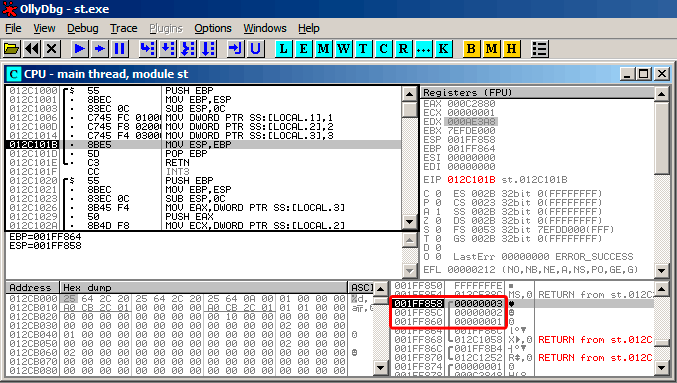
\includegraphics[scale=\FigScale]{patterns/02_stack/08_noise/olly1.png}
\caption{\olly: \TT{f1()}}
\label{fig:stack_noise_olly1}
\end{figure}

\RU{Когда}\EN{When} \TT{f1()} \RU{заполняет переменные}\EN{writes to} $a$, $b$ \AndENRU $c$ 
\RU{они сохранаяются по адресу}\EN{variables, they are stored at the address} \TT{0x14F85C} 
\RU{итд}\EN{and so on}.

\clearpage
\RU{А когда исполняется}\EN{And when} \TT{f2()}\EN{ executed}:

\begin{figure}[H]
\centering
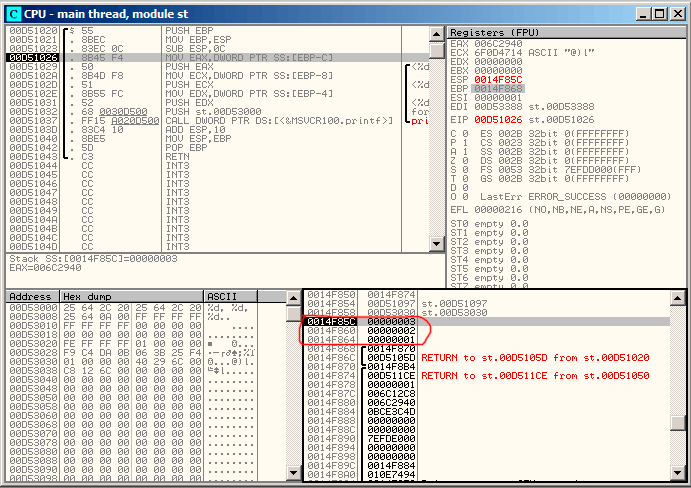
\includegraphics[scale=\FigScale]{patterns/02_stack/08_noise/olly2.png}
\caption{\olly: \TT{f2()}}
\label{fig:stack_noise_olly2}
\end{figure}

... $a$, $b$ \AndENRU $c$ \RU{в ф-ции}\EN{of} \TT{f2()} \RU{находятся по тем же адресам!}
\EN{are located at the same address!}
\RU{Пока никто не перезаписал их, так что они здесь в нетронутом виде.}
\EN{No one overwritten values yet, so they are still untouched here.}

\RU{Так что, для такой странной ситуации, несколько ф-ций должны исполняться друг за другом,
и \ac{SP} должен быть таким же при входе в ф-цию (т.е., у них должно быть равное кол-во
аргументов). Тогда, локальные переменные будут расположены в том же месте стека.}
\EN{So, for this weird situation, several functions should be called one after another and
\ac{SP} should be the same at each function entry (i.e., they should has same number
of arguments). Then, local variables will be located at the same point of stack.}

\RU{Подводя итоги, все значения в стеке (да и памяти вообще) это значения оставшиеся от 
исполнения предыдущих ф-ций}\EN{Summarizing, all values in stack (and memory cells at all) 
has values left there from previous function executions}.
\RU{Строго говоря, они не случайны, они скорее непредсказуемы}\EN{They are not 
random in strict sense, but rather has unpredictable values}.

\RU{А как иначе}\EN{How else}?
\RU{Вероятно, было бы возможным очищать части стека перед исполнением каждой ф-ции,
но это слишком много лишней (и ненужной) работы.}
\EN{Probably, it would be possible to clear stack portions before each function execution,
but that's too much extra (and needless) work.}

\fi
\ifdefined\IncludeExercises
\section{\Exercises}

\begin{itemize}
	\item \url{http://challenges.re/51}
	\item \url{http://challenges.re/52}
\end{itemize}


\fi

\chapter{\PrintfSeveralArgumentsSectionName}

\RU{Попробуем теперь немного расширить пример \IT{\HelloWorldSectionName}~(\ref{sec:helloworld}),
написав в теле функции \main:}
\EN{Now let's extend the \IT{\HelloWorldSectionName}~(\ref{sec:helloworld}) example, replacing \printf in
the \main function body by this:}

\lstinputlisting[label=hw_c]{patterns/03_printf/1.c}

% sections
\section{x86: \RU{3 аргумента}\EN{3 arguments}}

\subsection{MSVC}

\RU{Компилируем при помощи MSVC 2010 Express, и в итоге получим:}
\EN{Let's compile it by MSVC 2010 Express and we got:}

\begin{lstlisting}
$SG3830	DB	'a=%d; b=%d; c=%d', 00H

...

	push	3
	push	2
	push	1
	push	OFFSET $SG3830
	call	_printf
	add	esp, 16					; 00000010H
\end{lstlisting}

\RU{Все почти то же, за исключением того, что теперь видно, что аргументы для \printf заталкиваются в стек в обратном порядке: самый первый аргумент заталкивается последним.}
\EN{Almost the same, but now we can see the \printf arguments are pushed onto the stack in reverse order. The first argument is pushed last.}

\RU{Кстати, вспомним что переменные типа \Tint в 32-битной системе, как известно, имеет ширину 32 бита, это 4 байта}
\EN{By the way, variables of \Tint type in 32-bit environment have 32-bit width, that is 4 bytes}.

\RU{Итак, у нас всего 4 аргумента. $4*4 = 16$ ~--- именно 16 байт занимают в стеке указатель на строку плюс еще 3 числа типа \Tint.}
\EN{So, we have here 4 arguments. $4*4 = 16$~---they occupy exactly 16 bytes in the stack: a 32-bit pointer to a string and 3 numbers of type \Tint.}

\index{x86!\Instructions!ADD}
\index{x86!\Registers!ESP}
\index{cdecl}
\RU{Когда при помощи инструкции \TT{``ADD ESP, X''} корректируется \glslink{stack pointer}{указатель стека} \ESP 
после вызова какой-либо функции, зачастую можно сделать вывод о том, сколько аргументов 
у вызываемой функции было, разделив X на 4.}
\EN{When the \gls{stack pointer} (\ESP register) is changed back by the \TT{``ADD ESP, X''}
instruction after a function 
call, often, the number of function arguments can be deduced here: just divide X by 4.}

\RU{Конечно, это относится только к cdecl-методу передачи аргументов через стек.}
\EN{Of course, this is specific to the \IT{cdecl} calling convention.}

\RU{См. также в соответствующем разделе о способах передачи аргументов через стек}
\EN{See also the section about calling conventions}~(\ref{sec:callingconventions}).

\RU{Иногда бывает так, что подряд идут несколько вызовов разных функций, 
но стек корректируется только один раз, после последнего вызова:}
\EN{It is also possible for the compiler to merge several \TT{``ADD ESP, X''} instructions into one, after the last call:}

\begin{lstlisting}
push a1
push a2
call ...
...
push a1
call ...
...
push a1
push a2
push a3
call ...
add esp, 24
\end{lstlisting}

\subsection{MSVC \AndENRU \olly}
\index{\olly}

\RU{Попробуем этот же пример в}\EN{Now let's try to load this example in} \olly.
\RU{Это один из наиболее популярных win32-отладчиков user-режима}\EN{It is one of the most 
popular user-land win32 debugger}.
\RU{Мы можем компилировать наш пример в}\EN{We can try to compile our example in} MSVC 2012 
\RU{с опцией}\EN{with} \TT{/MD} \RU{что означает, линковать с библиотекой}\EN{option, meaning, to link 
against} \TT{MSVCR*.DLL},
\RU{чтобы импортируемые ф-ции были хорошо видны в отладчике}\EN{so we will able to see imported 
functions clearly in the debugger}.

\RU{Затем загружаем исполняемый файл в}\EN{Then load executable in} \olly.
\RU{Самый первый брякпойнт в}\EN{The very first breakpoint is in} \TT{ntdll.dll}, \RU{нажмите}\EN{press} 
F9 (\RU{запустить}\EN{run}).
\RU{Второй брякпойнт в}\EN{The second breakpoint is in} \ac{CRT}-\RU{коде}\EN{code}.
\RU{Теперь мы должны найти ф-цию}\EN{Now we should find the} \main\EN{ function}.

\RU{Найдите этот код скроллируя окно кода до самого верха (MSVC располагает ф-цию \main в самом начале
секции кода)}\EN{Find this code by scrolling the code to the very top (MSVC allocates \main function at
the very beginning of the code section)}: 
\figref{fig:printf3_olly_1}.\\
\\
\RU{Кликните на инструкции}\EN{Click on the} \TT{PUSH EBP}\RU{, нажмите}\EN{ instruction, press} F2 
(\RU{установка брякпойнта}\EN{set breakpoint}) \RU{и нажмите}\EN{and press} F9 (\RU{запустить}\EN{run}).
\RU{Нам нужно произвести все эти манипуляции, чтобы пропустить \ac{CRT}-код, потому что нам он пока
не интересен}\EN{We need to do these manipulations in order to skip \ac{CRT}-code, because, we aren't really
interested in it, yet}.\\
\\
\RU{Нажмите}\EN{Press} F8 (\stepover) 6 \RU{раз, т.е., пропустить
6 инструкций}\EN{times, i.e., skip 6 instructions}: \figref{fig:printf3_olly_2}.\\
\\
\RU{Теперь}\EN{Now the} \ac{PC} \RU{указывает на инструкцию}\EN{points to the}
\TT{CALL printf}\EN{ instruction}.
\olly, \RU{как и другие отладчики, подсвечивает регистры со значениями, которые изменились}
\EN{like other debuggers, highlights value of registers which were changed}.
\RU{Так что, каждый раз, когда мы нажимаем}\EN{So each time you press F8}, \EIP 
\RU{изменяется и его значение подсвечивается красным}\EN{ changes and its value looks red}.
\ESP \RU{также меняется, потому что значения заталкиваются в стек}\EN{changes as well, 
because values are pushed into the stack}.\\
\\
\RU{Где находятся эти значения в стеке}\EN{Where are the values in the stack}?
\RU{Посмотрите на правое/нижнее окно в отладчике}\EN{Take a look at the right/bottom window of debugger}:

\begin{figure}[H]
\centering
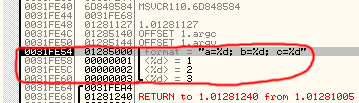
\includegraphics[scale=0.66]{patterns/03_printf/olly3_stack.png}
\caption{\olly: \RU{стек, после того как значения там сохранены}\EN{stack after values pushed}
(\RU{я сделал здесь округлую красную пометку в графическом редакторе}\EN{I made the round red mark 
here in a graphics editor})}
\end{figure}

\RU{Так что здесь видно 3 столбца: адрес в стеке, значение в стеке и еще дополнительный комментарий
от \olly}\EN{So we can see 3 columns there: address in the stack, 
value in the stack and some additional \olly comments}. 
\olly \RU{понимает}\EN{understands} \printf\RU{-строки}\EN{-like strings}, 
\RU{так что он показывает здесь и строку и 3 значения \IT{привязанных} к ней}\EN{so it reports the 
string here and 3 values \IT{attached} to it}.

\RU{Можно кликнуть правой кнопкой мыши на строке формата, кликнуть на ``Follow in dump''
и строка формата появится в окне слева внизу, где всегда виден какой-либо участок памяти}
\EN{It is possible to right-click on the format string, click on ``Follow in dump'',
and the format string will appear in the window at the left-bottom part, where some memory part
is always seen}.
\RU{Эти значения в памяти можно редактировать}\EN{These memory values can be edited}.
\RU{Можно изменить саму строку формата, и тогда результат работы нашего примера будет другой}
\EN{It is possible to change the format string, and then the result of our example will be different}.
\RU{В данном случае, пользы от этого немного, но для упражнения это полезно,
чтобы начать чувствовать как тут всё работает}\EN{It is probably not very useful now, but it's a very
good idea for doing it as an exercise, to get a feeling of how everything works here}.

\RU{Нажмите}\EN{Press} F8 (\stepover).

\RU{В консоли мы видим вывод}\EN{In the console we'll see the output}:

\begin{figure}[H]
\centering
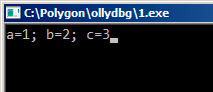
\includegraphics[scale=0.66]{patterns/03_printf/olly3_console.png}
\caption{\RU{Ф-ция }\printf \RU{исполнилась}\EN{function executed}}
\end{figure}

\RU{Посмотрим, как изменились регистры и состояние стека}\EN{Let's see how registers and stack state 
are changed}: \figref{fig:printf3_olly_3}.

\RU{Регистр }\EAX \RU{теперь содержит}\EN{register now contains} \TT{0xD} (13).
That's correct, since \printf returns the number of characters printed. The
\RU{Значение }\EIP \RU{изменилось: действительно, теперь здесь адрес инструкции после}
\EN{value is changed: indeed, now there is the address of the instruction after} \TT{CALL printf}.
\RU{Значения регистров }\ECX \AndENRU \EDX \RU{также изменились}\EN{values are changed as well}.
\RU{Очевидно, внутренности ф-ции \printf используют их для каких-то своих нужд}\EN{Apparently, 
\printf function's hidden machinery used them for its own needs}.

\RU{Очень важный момент в том что значение \ESP не изменилось. И аргменты-значения в стеке также!}
\EN{A very important fact is that neither the \ESP value, nor the stack state is changed!}
\RU{Мы ясно видим здесь и строку формата и соответствующие ей 3 значения, они все еще здесь.}
\EN{We clearly see that the format string and corresponding 3 values are still there.}
\RU{Действительно, по соглашению вызовов \IT{cdecl}, вызываемая ф-ция не возвращает \ESP назад.}
\EN{Indeed, that's the \IT{cdecl} calling convention: \gls{callee} doesn't return \ESP back to its previous value.}
\RU{Это должна делать вызывающая ф-ция}\EN{It's the \gls{caller}'s duty to do so}.

\RU{Нажмите}\EN{Press} F8 \RU{снова, чтобы исполнилась инструкция}\EN{again to execute} 
\TT{ADD ESP, 10}\EN{ instruction}: \figref{fig:printf3_olly_4}.

\ESP \RU{изменился, но значения все еще в стеке}\EN{is changed, but the values are still in the stack}!
\RU{Конечно, никому не нужно заполнять эти значения нулями или что-то в этом роде}\EN{Yes, 
of course; no one needs to fill these values by zero or something like that}.
\RU{Потому что всё что выше указателя стека}\EN{Because everything above stack pointer} (\ac{SP}) 
\RU{это}\EN{is} \IT{\RU{шум}\EN{noise}} \OrENRU \IT{\RU{мусор}\EN{garbage}}, \RU{это всё не имеет
особой ценности}\EN{and has no meaning at all}.
\RU{Было бы очень затратно по времени очищать ненужные элементы стека, к тому же, никому это и не 
нужно}\EN{It would be time consuming to clear unused stack entries anyways, and no one really needs to}.

\begin{figure}[H]
\centering
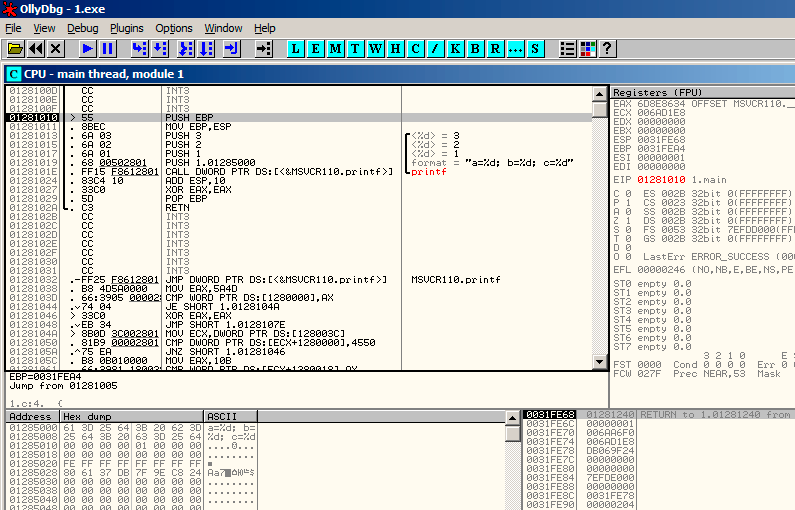
\includegraphics[scale=\FigScale]{patterns/03_printf/olly3_1.png}
\caption{\olly: \RU{самое начало ф-ции}\EN{the very start of the} \main\EN{ function}}
\label{fig:printf3_olly_1}
\end{figure}

\begin{figure}[H]
\centering
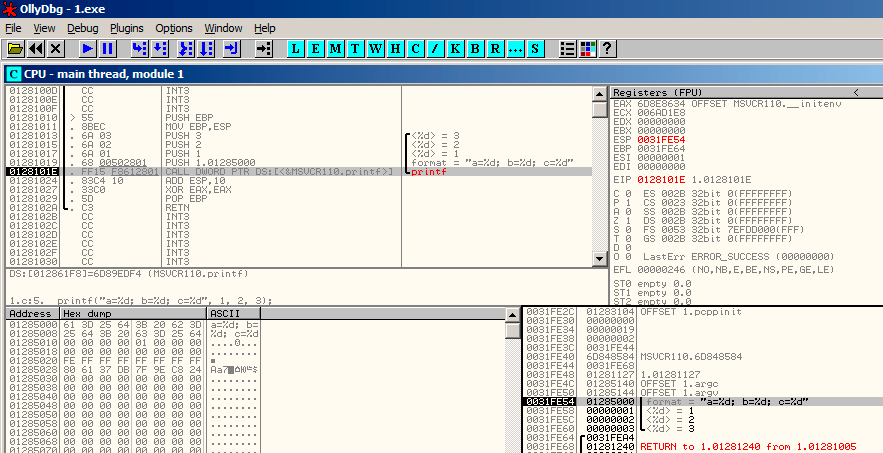
\includegraphics[scale=\FigScale]{patterns/03_printf/olly3_2.png}
\caption{\olly: \RU{перед исполнением}\EN{before} \printf\EN{ execution}}
\label{fig:printf3_olly_2}
\end{figure}

\begin{figure}[H]
\centering
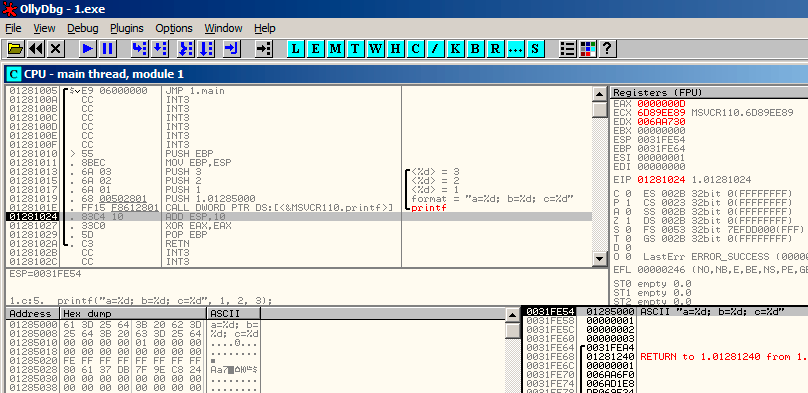
\includegraphics[scale=\FigScale]{patterns/03_printf/olly3_3.png}
\caption{\olly: \RU{после исполнения}\EN{after} \printf\EN{ execution}}
\label{fig:printf3_olly_3}
\end{figure}

\begin{figure}[H]
\centering
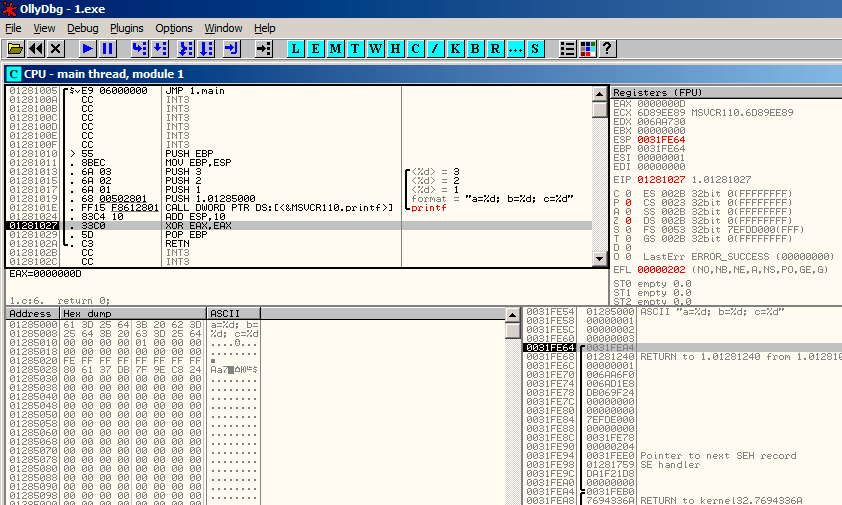
\includegraphics[scale=\FigScale]{patterns/03_printf/olly3_4.png}
\caption{\olly: \RU{после исполнения инструкции}\EN{after} \TT{ADD ESP, 10}\EN{ instruction execution}}
\label{fig:printf3_olly_4}
\end{figure}

\subsection{GCC}

\RU{Скомпилируем то же самое в Linux при помощи GCC 4.4.1 и посмотрим в \IDA что вышло:}
\EN{Now let's compile the same program in Linux using GCC 4.4.1 and take a look in \IDA what we got:}

\begin{lstlisting}
main            proc near

var_10          = dword ptr -10h
var_C           = dword ptr -0Ch
var_8           = dword ptr -8
var_4           = dword ptr -4

                push    ebp
                mov     ebp, esp
                and     esp, 0FFFFFFF0h
                sub     esp, 10h
                mov     eax, offset aADBDCD ; "a=%d; b=%d; c=%d"
                mov     [esp+10h+var_4], 3
                mov     [esp+10h+var_8], 2
                mov     [esp+10h+var_C], 1
                mov     [esp+10h+var_10], eax
                call    _printf
                mov     eax, 0
                leave
                retn
main            endp
\end{lstlisting}

\RU{Можно сказать, что этот короткий код, созданный GCC, отличается от кода MSVC только способом помещения 
значений в стек.
Здесь GCC снова работает со стеком напрямую без \PUSH/\POP.}
\EN{It can be said that the difference between code from MSVC and code from GCC is only in the method of placing arguments on the stack.
Here GCC is working directly with the stack without \PUSH/\POP.}

\subsection{GCC \AndENRU GDB}
\index{GDB}

\RU{Попробуем также этот пример и в \ac{GDB} в Linux}\EN{Let's try this example also in \ac{GDB} in Linux}.

\TT{-g} \RU{означает генерировать отладочную информацию в выходном исполняемом файле}\EN{mean produce 
debug information into executable file}.

\begin{lstlisting}
$ gcc 1.c -g -o 1
\end{lstlisting}

\begin{lstlisting}
$ gdb 1
GNU gdb (GDB) 7.6.1-ubuntu
Copyright (C) 2013 Free Software Foundation, Inc.
License GPLv3+: GNU GPL version 3 or later <http://gnu.org/licenses/gpl.html>
This is free software: you are free to change and redistribute it.
There is NO WARRANTY, to the extent permitted by law.  Type "show copying"
and "show warranty" for details.
This GDB was configured as "i686-linux-gnu".
For bug reporting instructions, please see:
<http://www.gnu.org/software/gdb/bugs/>...
Reading symbols from /home/dennis/polygon/1...done.
\end{lstlisting}

\begin{lstlisting}[caption=\RU{установим брякпойнт на}\EN{let's set breakpoint on} \printf]
(gdb) b printf
Breakpoint 1 at 0x80482f0
\end{lstlisting}

\RU{Запукаем}\EN{Run}.
\RU{Здесь у нас нет исходного кода ф-ции}\EN{There are no} \printf 
\RU{так что \ac{GDB} не может показать его исходный код, но могла бы}\EN{function source code here, 
so \ac{GDB} can't show its source, but may do so}.

\begin{lstlisting}
(gdb) run
Starting program: /home/dennis/polygon/1 

Breakpoint 1, __printf (format=0x80484f0 "a=%d; b=%d; c=%d") at printf.c:29
29	printf.c: No such file or directory.
\end{lstlisting}

\RU{Выдать 10 элементов стека. Левый столбец это адрес в стеке.}
\EN{Print 10 stack elements. The left column is an address in stack.}

\begin{lstlisting}
(gdb) x/10w $esp
0xbffff11c:	0x0804844a	0x080484f0	0x00000001	0x00000002
0xbffff12c:	0x00000003	0x08048460	0x00000000	0x00000000
0xbffff13c:	0xb7e29905	0x00000001
\end{lstlisting}

\RU{Самый первый элемент это}\EN{The very first element is the} \ac{RA} (\TT{0x0804844a}).
\RU{Мы можем удостовериться в этом, дизассемблируя память по этому адресу}\EN{We can make sure 
by disassembling the memory at this address}:

\begin{lstlisting}
(gdb) x/5i 0x0804844a
   0x804844a <main+45>:	mov    $0x0,%eax
   0x804844f <main+50>:	leave  
   0x8048450 <main+51>:	ret    
   0x8048451:	xchg   %ax,%ax
   0x8048453:	xchg   %ax,%ax
\end{lstlisting}

\RU{Две инструкции}\EN{Two} \TT{XCHG} 
\RU{это, вероятно, какой-то случайный мусор, который мы пока что можем игнорировать}
\EN{instructions, apparently, is some random garbage, which we can ignore so far}.

\RU{Второй элемент}\EN{The second element} (\TT{0x080484f0}) \RU{это адрес
строки формата}\EN{is an address of format string}:

\begin{lstlisting}
(gdb) x/s 0x080484f0
0x80484f0:	"a=%d; b=%d; c=%d"
\end{lstlisting}

\RU{Остальные 3 элемента}\EN{Other 3 elements} (1, 2, 3) \RU{это аргументы ф-ции}\EN{are} 
\printf\EN{ arguments}.
\RU{Остальные элементы это может быть и мусор в стеке, но могут быть и значения
от других ф-ций, их локальные переменные, итд}\EN{Other elements may be just ``garbage'' present in stack,
but also may be values from other functions, their local variables, etc}.
\RU{Пока что мы можем игнорировать их}\EN{We can ignore it for now}.

\RU{Исполняем}\EN{Execute} ``finish''. 
\RU{Это значит, исполнять до конца ф-ции}\EN{This mean, execute till function end}. 
\RU{Здесь это означает: исполнять до завершения}\EN{Here it means: execute till the finish of} \printf.

\begin{lstlisting}
(gdb) finish
Run till exit from #0  __printf (format=0x80484f0 "a=%d; b=%d; c=%d") at printf.c:29
main () at 1.c:6
6		return 0;
Value returned is $2 = 13
\end{lstlisting}

\ac{GDB} \RU{показывает, что вернула}\EN{shows what} \printf \RU{в}\EN{returned in} \EAX (13).
\RU{Это, так же как и в примере с \olly, количество напечатанных символов}
\EN{This is number of characters printed, just like in the example with \olly}.

\RU{А еще мы видим}\EN{We also see} ``return 0;'' \RU{и что это выражение находится в файле 
\TT{1.c} в строке 6}\EN{and the information that this expression is in the \TT{1.c} file at the line 6}.
\RU{Действительно, файл \TT{1.c} лежит в текущем директории и \ac{GDB} находит там эту строку}
\EN{Indeed, the \TT{1.c} file is located in the current directory, and \ac{GDB} finds the string there}.
\RU{Как \ac{GDB} знает, какая строка Си-кода сейчас исполняется}\EN{How does \ac{GDB} know which C-code line
is being executed now}?
\RU{Это связано с тем фактом, что компилятор, генерируя отладочную информацию,
также сохраняет информацию о 
соответствии строк в исходном коде и адресов инструкций}\EN{This is due to the fact that the compiler,
while generating debugging information, also saves a table of relations between source code line
numbers and instruction addresses}.
GDB \RU{это всё-таки отладчик уровня исходных текстов}\EN{is a source-level debugger, after all}.

\RU{Посмотрим регистры}\EN{Let's examine registers}.
13 \InENRU \EAX:

\begin{lstlisting}
(gdb) info registers
eax            0xd	13
ecx            0x0	0
edx            0x0	0
ebx            0xb7fc0000	-1208221696
esp            0xbffff120	0xbffff120
ebp            0xbffff138	0xbffff138
esi            0x0	0
edi            0x0	0
eip            0x804844a	0x804844a <main+45>
...
\end{lstlisting}

\RU{Попробуем дизассемблировать текущие инструкции}\EN{Let's disassemble the current instructions}.
\RU{Стрелка указывает на инструкцию, которая будет исполнена следующей}\EN{The arrow points to the 
instruction to be executed next}.

\begin{lstlisting}
(gdb) disas
Dump of assembler code for function main:
   0x0804841d <+0>:	push   %ebp
   0x0804841e <+1>:	mov    %esp,%ebp
   0x08048420 <+3>:	and    $0xfffffff0,%esp
   0x08048423 <+6>:	sub    $0x10,%esp
   0x08048426 <+9>:	movl   $0x3,0xc(%esp)
   0x0804842e <+17>:	movl   $0x2,0x8(%esp)
   0x08048436 <+25>:	movl   $0x1,0x4(%esp)
   0x0804843e <+33>:	movl   $0x80484f0,(%esp)
   0x08048445 <+40>:	call   0x80482f0 <printf@plt>
=> 0x0804844a <+45>:	mov    $0x0,%eax
   0x0804844f <+50>:	leave  
   0x08048450 <+51>:	ret    
End of assembler dump.
\end{lstlisting}

\ac{GDB} \RU{показывает дизассемблированный листинг в формате}\EN{shows disassembly in} AT\&T 
\RU{по умолчанию}\EN{syntax by default}.
\RU{Но можно также переключиться в формат Intel}\EN{It's possible to switch to Intel syntax}:

\begin{lstlisting}
(gdb) set disassembly-flavor intel
(gdb) disas
Dump of assembler code for function main:
   0x0804841d <+0>:	push   ebp
   0x0804841e <+1>:	mov    ebp,esp
   0x08048420 <+3>:	and    esp,0xfffffff0
   0x08048423 <+6>:	sub    esp,0x10
   0x08048426 <+9>:	mov    DWORD PTR [esp+0xc],0x3
   0x0804842e <+17>:	mov    DWORD PTR [esp+0x8],0x2
   0x08048436 <+25>:	mov    DWORD PTR [esp+0x4],0x1
   0x0804843e <+33>:	mov    DWORD PTR [esp],0x80484f0
   0x08048445 <+40>:	call   0x80482f0 <printf@plt>
=> 0x0804844a <+45>:	mov    eax,0x0
   0x0804844f <+50>:	leave  
   0x08048450 <+51>:	ret    
End of assembler dump.
\end{lstlisting}

\RU{Исполняем следующую инструкцию}\EN{Execute next instruction}.
\ac{GDB} \RU{покажет закрывающуюся скобку, означая, что это конец блока в ф-ции}\EN{shows ending bracket, 
meaning, this ends the block of the function}.

\begin{lstlisting}
(gdb) step
7	};
\end{lstlisting}

\RU{Посмотрим регистры после исполнения инструкции}\EN{Let's see the registers after the} 
\TT{MOV EAX, 0}\EN{ instruction execution}.
\EAX \RU{здесь уже действительно ноль}\EN{here is zero indeed}.

\begin{lstlisting}
(gdb) info registers
eax            0x0	0
ecx            0x0	0
edx            0x0	0
ebx            0xb7fc0000	-1208221696
esp            0xbffff120	0xbffff120
ebp            0xbffff138	0xbffff138
esi            0x0	0
edi            0x0	0
eip            0x804844f	0x804844f <main+50>
...
\end{lstlisting}

\section{x64: \RU{8 аргументов}\EN{8 arguments}}

\index{x86-64}
\label{example_printf8_x64}
\RU{Для того, чтобы посмотреть, как остальные аргументы будут передаваться через стек, 
изменим пример еще раз, 
увеличив количество передаваемых аргументов до 9 (строка формата \printf и 8 переменных типа \Tint)}
\EN{To see how other arguments will be passed via the stack, let's change our example again by increasing the number of arguments
to be passed to 9 (\printf format string + 8 \Tint variables)}:

\lstinputlisting{patterns/03_printf/2.c}

\subsection{MSVC}

\RU{Как уже было сказано раннее, первые 4 аргумента в Win64 передаются в регистрах}
\EN{As we saw before, the first 4 arguments are passed in the} \RCX, \RDX, \Reg{8}, \Reg{9}
\RU{, а остальные --- через стек}\EN{ registers in Win64, while all the rest---via the stack}.
\RU{Здесь мы это и видим}\EN{That is what we see here}.
\RU{Впрочем, инструкция \PUSH не используется, вместо нее, при помощи \MOV, значения сразу записываются в стек}
\EN{However, the \MOV instruction, instead of \PUSH, is used for preparing the stack, so the values are written
to the stack in a straightforward manner}.

\lstinputlisting[caption=MSVC 2012 x64]{patterns/03_printf/2_MSVC_x64.asm}

\RU{Наблюдательный читатель может спросить, почему для значений типа \Tint отводится 8 байт,
ведь нужно только 4?}
\EN{Observant reader may ask, what 8 bytes are allocated for \Tint values, while 4 is enough?}
\RU{Да, это нужно запомнить: для значений всех типов более коротких чем 64-бита, отводится 8 байт.}
\EN{Yes, this should be memorized: 8 bytes are allocated for any data type shorter than 64 bits.}
\RU{Это сделано для удобства: так всегда легко расчитать адрес того или иного аргумента.}
\EN{It's done for convenience: it's always easy to calculate address of this or that argument.}
\RU{К тому же, все они расположены по выровненным адресам в памяти.}
\EN{Besides, all they are located at aligned memory addresses.}
% also for local variables?
\RU{В 32-битных средах точно также: для всех типов резервируется 4 байта в стеке.}
\EN{The same story in 32-bit environments: 4 bytes are reserved for all data types.}

\subsection{GCC}

\RU{В *NIX-системах для x86-64 ситуация похожая, вот только первые 6 аргументов передаются через}
\EN{In *NIX OS-es, it's the same story for x86-64, except that the first 6 arguments are passed in the} \RDI, \RSI,
\RDX, \RCX, \Reg{8}, \Reg{9}\EN{ registers}.
\RU{Остальные --- через стек}\EN{All the rest---via the stack}.
\RU{GCC генерирует код записывающий указатель на строку в \EDI вместо \RDI --- 
это мы уже рассмотрели чуть раньше}\EN{GCC generates the code writing string pointer into \EDI instead if \RDI{}---we
saw this thing before}: \ref{hw_EDI_instead_of_RDI}.

\RU{Почему перед вызовом \printf очищается регистр \EAX, мы уже рассмотрели раннее}
\EN{We also saw before the \EAX register being cleared before a \printf call}: \ref{SysVABI_input_EAX}.

\lstinputlisting[caption=\Optimizing GCC 4.4.6 x64]{patterns/03_printf/2_GCC_x64_\LANG.s}

\ifdefined\IncludeGDB
\subsection{GCC + GDB}
\index{GDB}

\RU{Попробуем этот пример в}\EN{Let's try this example in} \ac{GDB}.

\begin{lstlisting}
$ gcc -g 2.c -o 2
\end{lstlisting}

\begin{lstlisting}
$ gdb 2
GNU gdb (GDB) 7.6.1-ubuntu
Copyright (C) 2013 Free Software Foundation, Inc.
License GPLv3+: GNU GPL version 3 or later <http://gnu.org/licenses/gpl.html>
This is free software: you are free to change and redistribute it.
There is NO WARRANTY, to the extent permitted by law.  Type "show copying"
and "show warranty" for details.
This GDB was configured as "x86_64-linux-gnu".
For bug reporting instructions, please see:
<http://www.gnu.org/software/gdb/bugs/>...
Reading symbols from /home/dennis/polygon/2...done.
\end{lstlisting}

\begin{lstlisting}[caption=\RU{ставим брякпойнт на \printf{,} запускаем}\EN{let's set the breakpoint to \printf{,} and run}]
(gdb) b printf
Breakpoint 1 at 0x400410
(gdb) run
Starting program: /home/dennis/polygon/2 

Breakpoint 1, __printf (format=0x400628 "a=%d; b=%d; c=%d; d=%d; e=%d; f=%d; g=%d; h=%d\n") at printf.c:29
29	printf.c: No such file or directory.
\end{lstlisting}

\RU{В регистрах}\EN{Registers} \RSI/\RDX/\RCX/\Reg{8}/\Reg{9} 
\RU{всё предсказуемо}\EN{has the values which are should be there}.
\RU{А }\RIP \RU{содержит адрес самой первой инструкции ф-ции}\EN{has an address of the very first instruction
of the} \printf\EN{ function}.

\begin{lstlisting}
(gdb) info registers
rax            0x0	0
rbx            0x0	0
rcx            0x3	3
rdx            0x2	2
rsi            0x1	1
rdi            0x400628	4195880
rbp            0x7fffffffdf60	0x7fffffffdf60
rsp            0x7fffffffdf38	0x7fffffffdf38
r8             0x4	4
r9             0x5	5
r10            0x7fffffffdce0	140737488346336
r11            0x7ffff7a65f60	140737348263776
r12            0x400440	4195392
r13            0x7fffffffe040	140737488347200
r14            0x0	0
r15            0x0	0
rip            0x7ffff7a65f60	0x7ffff7a65f60 <__printf>
...
\end{lstlisting}

\begin{lstlisting}[caption=\RU{смотрим на строку формата}\EN{let's inspect the format string}]
(gdb) x/s $rdi
0x400628:	"a=%d; b=%d; c=%d; d=%d; e=%d; f=%d; g=%d; h=%d\n"
\end{lstlisting}

\RU{Дампим стек на этот раз с командой x/g}\EN{Let's dump the stack with the x/g command this time}\EMDASH{}g 
\RU{означает}\EN{means} \IT{giant words}, \RU{т.е., 64-битные слова}\EN{i.e., 64-bit words}.

\begin{lstlisting}
(gdb) x/10g $rsp
0x7fffffffdf38:	0x0000000000400576	0x0000000000000006
0x7fffffffdf48:	0x0000000000000007	0x00007fff00000008
0x7fffffffdf58:	0x0000000000000000	0x0000000000000000
0x7fffffffdf68:	0x00007ffff7a33de5	0x0000000000000000
0x7fffffffdf78:	0x00007fffffffe048	0x0000000100000000
\end{lstlisting}

\RU{Самый первый элемент стека, как и в прошлый раз, это}\EN{The very first stack element, 
just like in the previous case, is the} \ac{RA}.
\RU{Через стек также передаются 3 значения}\EN{3 values are also passed in stack}: 6, 7, 8.
\RU{Видно, что 8 передается с не очищенной старшей 32-битной частью}\EN{We also see that 8 is passed
with high 32-bits not cleared}: \TT{0x00007fff00000008}.
\RU{Это нормально, ведь передаются числа типа \Tint, а они 32-битные}\EN{That's OK, because the values have
\Tint type, which is 32-bit type}.
\RU{Так что в старшей части регистра или памяти стека остался ``случайный мусор''}\EN{So, the high register
or stack element part may contain ``random garbage''}.

\RU{\ac{GDB} показывает всю ф-цию \main, если попытаться посмотреть, куда возвратится управление после
исполнения \printf}\EN{If you take a look at where control flow will return after \printf execution,
\ac{GDB} will show the whole \main function}:

\begin{lstlisting}
(gdb) set disassembly-flavor intel
(gdb) disas 0x0000000000400576
Dump of assembler code for function main:
   0x000000000040052d <+0>:	push   rbp
   0x000000000040052e <+1>:	mov    rbp,rsp
   0x0000000000400531 <+4>:	sub    rsp,0x20
   0x0000000000400535 <+8>:	mov    DWORD PTR [rsp+0x10],0x8
   0x000000000040053d <+16>:	mov    DWORD PTR [rsp+0x8],0x7
   0x0000000000400545 <+24>:	mov    DWORD PTR [rsp],0x6
   0x000000000040054c <+31>:	mov    r9d,0x5
   0x0000000000400552 <+37>:	mov    r8d,0x4
   0x0000000000400558 <+43>:	mov    ecx,0x3
   0x000000000040055d <+48>:	mov    edx,0x2
   0x0000000000400562 <+53>:	mov    esi,0x1
   0x0000000000400567 <+58>:	mov    edi,0x400628
   0x000000000040056c <+63>:	mov    eax,0x0
   0x0000000000400571 <+68>:	call   0x400410 <printf@plt>
   0x0000000000400576 <+73>:	mov    eax,0x0
   0x000000000040057b <+78>:	leave  
   0x000000000040057c <+79>:	ret    
End of assembler dump.
\end{lstlisting}

\RU{Заканчиваем исполнение \printf, исполняем инструкцию обнуляющую \EAX, 
удостоверяемся что в регистре \EAX именно ноль}\EN{Let's finish executing \printf, execute the instruction
zeroing \EAX, and note that the \EAX register has a value of exactly zero}.
\RIP \RU{указывает сейчас на инструкцию}\EN{now points to the} \TT{LEAVE}\RU{, т.е., предпоследнюю в ф-ции \main}
\EN{ instruction, i.e., the penultimate one in the \main function}.

\begin{lstlisting}
(gdb) finish
Run till exit from #0  __printf (format=0x400628 "a=%d; b=%d; c=%d; d=%d; e=%d; f=%d; g=%d; h=%d\n") at printf.c:29
a=1; b=2; c=3; d=4; e=5; f=6; g=7; h=8
main () at 2.c:6
6		return 0;
Value returned is $1 = 39
(gdb) next
7	};
(gdb) info registers
rax            0x0	0
rbx            0x0	0
rcx            0x26	38
rdx            0x7ffff7dd59f0	140737351866864
rsi            0x7fffffd9	2147483609
rdi            0x0	0
rbp            0x7fffffffdf60	0x7fffffffdf60
rsp            0x7fffffffdf40	0x7fffffffdf40
r8             0x7ffff7dd26a0	140737351853728
r9             0x7ffff7a60134	140737348239668
r10            0x7fffffffd5b0	140737488344496
r11            0x7ffff7a95900	140737348458752
r12            0x400440	4195392
r13            0x7fffffffe040	140737488347200
r14            0x0	0
r15            0x0	0
rip            0x40057b	0x40057b <main+78>
...
\end{lstlisting}
\fi

\ifdefined\IncludeARM
\subsection{ARM: \RU{3 аргумента}\EN{3 arguments}}

\RU{В ARM традиционно принята такая схема передачи аргументов в функцию: 
4 первых аргумента через регистры \Reg{0}-\Reg{3}; а остальные~--- через стек}
\EN{ARM's traditional scheme for passing arguments (calling convention) behaves as follows:
the first 4 arguments are passed through the \Reg{0}-\Reg{3} registers; the remaining arguments via the stack}.
\RU{Это немного похоже на то, как аргументы передаются в}\EN{This resembles the arguments passing scheme in} 
fastcall~(\myref{fastcall}) \OrENRU win64~(\myref{sec:callingconventions_win64}).

\subsubsection{32-\RU{битный}\EN{bit} ARM}

\myparagraph{\NonOptimizingKeilVI (\ARMMode)}

\begin{lstlisting}[caption=\NonOptimizingKeilVI (\ARMMode)]
.text:00000000 main
.text:00000000 10 40 2D E9   STMFD   SP!, {R4,LR}
.text:00000004 03 30 A0 E3   MOV     R3, #3
.text:00000008 02 20 A0 E3   MOV     R2, #2
.text:0000000C 01 10 A0 E3   MOV     R1, #1
.text:00000010 08 00 8F E2   ADR     R0, aADBDCD     ; "a=%d; b=%d; c=%d"
.text:00000014 06 00 00 EB   BL      __2printf
.text:00000018 00 00 A0 E3   MOV     R0, #0          ; return 0
.text:0000001C 10 80 BD E8   LDMFD   SP!, {R4,PC}
\end{lstlisting}

\RU{Итак, первые 4 аргумента передаются через регистры \Reg{0}-\Reg{3}, по порядку: 
указатель на формат-строку для \printf
в \Reg{0}, затем 1 в \Reg{1}, 2 в \Reg{2} и 3 в \Reg{3}}
\EN{So, the first 4 arguments are passed via the \Reg{0}-\Reg{3} registers in this order:
a pointer to the \printf format string in 
\Reg{0}, then 1 in \Reg{1}, 2 in \Reg{2} and 3 in \Reg{3}}.

\RU{Инструкция на}\EN{The instruction at} \TT{0x18} \RU{записывает}\EN{writes} 0 \RU{в}\EN{to} \Reg{0}
\EMDASH{}\RU{это выражение в Си}\EN{this is} \IT{return 0}\EN{ C-statement}.

\RU{Пока что здесь нет ничего необычного}\EN{There is nothing unusual so far}.

\OptimizingKeilVI \RU{генерирует точно такой же код}\EN{generates the same code}.

\myparagraph{\OptimizingKeilVI (\ThumbMode)}

\begin{lstlisting}[caption=\OptimizingKeilVI (\ThumbMode)]
.text:00000000 main
.text:00000000 10 B5        PUSH    {R4,LR}
.text:00000002 03 23        MOVS    R3, #3
.text:00000004 02 22        MOVS    R2, #2
.text:00000006 01 21        MOVS    R1, #1
.text:00000008 02 A0        ADR     R0, aADBDCD     ; "a=%d; b=%d; c=%d"
.text:0000000A 00 F0 0D F8  BL      __2printf
.text:0000000E 00 20        MOVS    R0, #0
.text:00000010 10 BD        POP     {R4,PC}
\end{lstlisting}

\RU{Здесь нет особых отличий от неоптимизированного варианта для режима ARM}
\EN{There is no significant difference from the non-optimized code for ARM mode}.

\myparagraph{\OptimizingKeilVI (\ARMMode) + \RU{убираем}\EN{let's remove} return}
\label{ARM_B_to_printf}

\RU{Немного переделаем пример, убрав}\EN{Let's rework example slightly by removing} \IT{return 0}:

\begin{lstlisting}
#include <stdio.h>

void main()
{
	printf("a=%d; b=%d; c=%d", 1, 2, 3);
};
\end{lstlisting}

\RU{Результат получится необычным:}
\EN{The result is somewhat unusual:}

\begin{lstlisting}[caption=\OptimizingKeilVI (\ARMMode)]
.text:00000014 main
.text:00000014 03 30 A0 E3   MOV     R3, #3
.text:00000018 02 20 A0 E3   MOV     R2, #2
.text:0000001C 01 10 A0 E3   MOV     R1, #1
.text:00000020 1E 0E 8F E2   ADR     R0, aADBDCD     ; "a=%d; b=%d; c=%d\n"
.text:00000024 CB 18 00 EA   B       __2printf
\end{lstlisting}

\index{ARM!\Registers!Link Register}
\index{ARM!\Instructions!B}
\index{Function epilogue}
\RU{Это оптимизированная версия (\Othree) для режима ARM, и здесь мы видим последнюю инструкцию 
\TT{B} вместо привычной нам \TT{BL}}\EN{This is the optimized (\Othree) version for ARM mode and this time we see \TT{B} as the last instruction instead of the familiar \TT{BL}}.
\RU{Отличия между этой оптимизированной версией и предыдущей, скомпилированной без оптимизации, 
ещё и в том, 
что здесь нет пролога и эпилога функции (инструкций, сохраняющих состояние регистров \TT{\Reg{0}} и \ac{LR})}%
\EN{Another difference between this optimized version and the previous one (compiled without optimization)
is the lack of function prologue and epilogue (instructions preserving the \TT{\Reg{0}} and \ac{LR} registers values)}.
\index{x86!\Instructions!JMP}
\RU{Инструкция \TT{B} просто переходит на другой адрес, без манипуляций с регистром \ac{LR}, то есть
это аналог \JMP в x86}%
\EN{The \TT{B} instruction just jumps to another address, without any manipulation of the \ac{LR} register,
similar to \JMP in x86}.
\RU{Почему это работает нормально? Потому что этот код эквивалентен предыдущему.}
\EN{Why does it work? Because this code is, in fact, effectively equivalent to the previous.}
\RU{Основных причин две: 1) стек не модифицируется, как и \glslink{stack pointer}{указатель стека} \ac{SP}; 2) вызов функции \printf последний, 
после него ничего не происходит}\EN{There are two main reasons: 1) neither the stack nor \ac{SP} (the \gls{stack pointer}) is modified;
2) the call to \printf is the last instruction, so there is nothing going on afterwards}.
\RU{Функция \printf, отработав, просто возвращает управление по адресу, записанному в \ac{LR}.}
\EN{On completion, the \printf function simply returns the control to the address 
stored in \ac{LR}.}
\RU{Но в \ac{LR} находится адрес места, откуда была вызвана наша функция!
А следовательно, управление из \printf вернется сразу туда.}
\EN{Since the \ac{LR} currently stores the address of the point from where our function
was called then the control from \printf will be returned to that point.}
\RU{Значит нет нужды сохранять \ac{LR}, потому что нет нужны модифицировать \ac{LR}}%
\EN{Therefore we do not need to save \ac{LR} because we do not need to modify \ac{LR}}.
\RU{А нет нужды модифицировать \ac{LR}, потому что нет иных вызовов функций, кроме \printf, к тому же, после этого вызова не нужно ничего здесь больше делать}%
\EN{And we do not need to modify \ac{LR} because there are no other function calls except \printf. Furthermore,
after this call we do not to do anything else}!
\RU{Поэтому такая оптимизация возможна}\EN{That is the reason such optimization is possible}.

\RU{Эта оптимизация часто используется в функциях, где последнее выражение~--- это вызов другой функции.}
\EN{This optimization is often used in functions where the last statement is a call to another function.}

\RU{Ещё один похожий пример описан здесь}\EN{A similar example is presented here}:
\myref{jump_to_last_printf}.

\subsubsection{ARM64}

\myparagraph{\NonOptimizing GCC (Linaro) 4.9}

\lstinputlisting[caption=\NonOptimizing GCC (Linaro) 4.9]{patterns/03_printf/ARM/ARM3_O0.lst.\LANG}

\index{ARM!\Instructions!STP}
\RU{Итак, первая инструкция STP (Store Pair) сохраняет \ac{FP} (X29) и \ac{LR} (X30) в стеке.}
\EN{The first instruction STP (Store Pair) saves \ac{FP} (X29) and \ac{LR} (X30) in the stack.}
\RU{Вторая инструкция \TT{ADD X29, SP, 0} формирует стековый фрейм.}
\EN{The second \TT{ADD X29, SP, 0} instruction forms the stack frame.}
\RU{Это просто запись значения \ac{SP} в X29.}
\EN{It is just writing the value of \ac{SP} into X29.}

\index{ARM!\Instructions!ADRP/ADD pair}
\RU{Далее уже знакомая пара инструкций \TT{ADRP}/\ADD формирует указатель на строку.}
\EN{Next, we see the familiar \TT{ADRP}/\ADD instruction pair, which forms a pointer to the string.}

\RU{\TT{\%d} в формате \printf это 32-битный \Tint, так что 1, 2 и 3 заносятся в 32-битные части регистров.}
\EN{\TT{\%d} in \printf string format is a 32-bit \Tint, so the 1, 2 and 3 are loaded into 32-bit register parts.}

\Optimizing GCC (Linaro) 4.9 \RU{генерирует почти такой же код}\EN{generates the same code}.

\subsection{ARM: \RU{8 аргументов}\EN{8 arguments}}

\RU{Снова воспользуемся примером с 9-ю аргументами из предыдущей секции}\EN{Let's use again the example
with 9 arguments from the previous section}: \myref{example_printf8_x64}.

\lstinputlisting{patterns/03_printf/2.c}

\subsubsection{\OptimizingKeilVI: \ARMMode}

\begin{lstlisting}
.text:00000028             main
.text:00000028
.text:00000028             var_18 = -0x18
.text:00000028             var_14 = -0x14
.text:00000028             var_4  = -4
.text:00000028
.text:00000028 04 E0 2D E5  STR    LR, [SP,#var_4]!
.text:0000002C 14 D0 4D E2  SUB    SP, SP, #0x14
.text:00000030 08 30 A0 E3  MOV    R3, #8
.text:00000034 07 20 A0 E3  MOV    R2, #7
.text:00000038 06 10 A0 E3  MOV    R1, #6
.text:0000003C 05 00 A0 E3  MOV    R0, #5
.text:00000040 04 C0 8D E2  ADD    R12, SP, #0x18+var_14
.text:00000044 0F 00 8C E8  STMIA  R12, {R0-R3}
.text:00000048 04 00 A0 E3  MOV    R0, #4
.text:0000004C 00 00 8D E5  STR    R0, [SP,#0x18+var_18]
.text:00000050 03 30 A0 E3  MOV    R3, #3
.text:00000054 02 20 A0 E3  MOV    R2, #2
.text:00000058 01 10 A0 E3  MOV    R1, #1
.text:0000005C 6E 0F 8F E2  ADR    R0, aADBDCDDDEDFDGD ; "a=%d; b=%d; c=%d; d=%d; e=%d; f=%d; g=%"...
.text:00000060 BC 18 00 EB  BL     __2printf
.text:00000064 14 D0 8D E2  ADD    SP, SP, #0x14
.text:00000068 04 F0 9D E4  LDR    PC, [SP+4+var_4],#4
\end{lstlisting}

\RU{Этот код можно условно разделить на несколько частей}\EN{This code can be divided into several parts}:

\begin{itemize}
\index{Function prologue}
\item \RU{Пролог функции}\EN{Function prologue}:

\index{ARM!\Instructions!STR}
\RU{Самая первая инструкция}\EN{The very first} \TT{STR LR, [SP,\#var\_4]!} 
\RU{сохраняет в стеке \ac{LR}, ведь нам придется использовать этот регистр для вызова \printf}%
\EN{instruction saves \ac{LR} on the stack, because we are going to use this register for the \printf call}.
\RU{Восклицательный знак в конце означает}\EN{Exclamation mark at the end indicates} \IT{pre-index}.
\RU{Это значит, что в начале \ac{SP} должно быть
уменьшено на 4, затем по адресу в \ac{SP} должно быть записано значение \ac{LR}.}
\EN{This implies that \ac{SP} is to be decreased by 4 first, and then \ac{LR} will be saved at the address stored in \ac{SP}.}
\RU{Это аналог знакомой в x86 инструкции \PUSH}\EN{This is similar to \PUSH in x86}.
\RU{Читайте больше об этом}\EN{Read more about it at}: \myref{ARM_postindex_vs_preindex}.

\index{ARM!\Instructions!SUB}
\RU{Вторая инструкция}\EN{The second} \TT{SUB SP, SP, \#0x14}
\RU{уменьшает \glslink{stack pointer}{указатель стека} \ac{SP}, но, на самом деле, эта процедура нужна для выделения в локальном стеке места размером \TT{0x14} (20) байт.}
\EN{instruction decreases
\ac{SP} (the \gls{stack pointer}) in order to 
allocate \TT{0x14} (20) bytes on the stack.}
\RU{Действительно, нам нужно передать 5 32-битных значений через стек в \printf. Каждое значение занимает 4 байта, все вместе~--- $5*4=20$.}
\EN{Indeed, we need to pass 5 32-bit values via the stack to the \printf function, and each one occupies 4 bytes, which is exactly $5*4=20$.}
\RU{Остальные 4 32-битных значения будут переданы через регистры.}
\EN{The other 4 32-bit values are to be passed through registers.}

\item \RU{Передача 5, 6, 7 и 8 через стек}\EN{Passing 5, 6, 7 and 8 via the stack}:
\RU{они записываются в регистры \Reg{0}, \Reg{1}, \Reg{2} и \Reg{3} соответственно}%
\EN{they are stored in the \Reg{0}, \Reg{1}, \Reg{2} and \Reg{3} registers respectively}.
\RU{Затем инструкция}\EN{Then, the} \TT{ADD R12, SP, \#0x18+var\_14} 
\RU{записывает в регистр \TT{R12} адрес места в стеке, куда будут помещены эти 4 значения}%
\EN{instruction writes the stack address where these 4 variables are to be stored, into the \TT{R12} register}.
\index{IDA!var\_?}
\IT{var\_14}\RU{~--- это макрос ассемблера}\EN{ is an assembly macro}, \RU{равный}\EN{equal to} -0x14\RU{.}
\RU{Такие макросы создает \IDA, чтобы удобнее было показывать, как код обращается к стеку.}
\EN{, created by \IDA to conveniently display the code accessing the stack.}
\RU{Макросы \IT{var\_?}, создаваемые \IDA, отражают локальные переменные в стеке}\EN{The \IT{var\_?} macros generated
by \IDA reflect local variables in the stack.}
\RU{Так что в \TT{R12} будет записано \TT{SP+4}.}
\EN{So, \TT{SP+4} is to be stored into the \TT{R12} register.}
\index{ARM!\Instructions!STMIA}
\RU{Следующая инструкция}\EN{The next} \TT{STMIA R12, {R0-R3}} 
\RU{записывает содержимое регистров \Reg{0}-\Reg{3} по адресу в памяти, на который указывает \TT{R12}.}
\EN{instruction
writes registers \Reg{0}-\Reg{3} contents to the memory pointed by \TT{R12}.}
\RU{Инструкция }\TT{STMIA} \RU{означает}\EN{abbreviates} \IT{Store Multiple Increment After}. 
\IT{\q{Increment After}} 
\RU{означает, что \TT{R12} будет увеличиваться на 4 после записи каждого значения регистра.}
\EN{implies that \TT{R12} is to be increased by 4 after each register value is written.}

\item \RU{Передача 4 через стек}\EN{Passing 4 via the stack}:
\RU{4 записывается в \Reg{0}, затем инструкция}\EN{4 is stored in \Reg{0} and then
this value, with the help of the} \TT{STR R0, [SP,\#0x18+var\_18]} \RU{записывает его в стек}\EN{instruction is saved
on the stack}.
\IT{var\_18} \RU{равен}\EN{is} -0x18, \RU{смещение будет 0}\EN{so the offset is to be 0}, 
\RU{так что значение из регистра \Reg{0} (4) запишется туда, куда указывает \ac{SP}}%
\EN{thus the value from the \Reg{0} register (4) is to be written to the address written in \ac{SP}}.

\item \RU{Передача 1, 2 и 3 через регистры}\EN{Passing 1, 2 and 3 via registers}:

\RU{Значения для первых трех чисел (a, b, c) (1, 2, 3 соответственно) передаются в регистрах 
\Reg{1}, \Reg{2} и \Reg{3} перед самим вызовом \printf}%
\EN{The values of the first 3 numbers (a, b, c) (1, 2, 3 respectively) are passed through the 
\Reg{1}, \Reg{2} and \Reg{3}
registers right before the \printf call}, \RU{а остальные 5 значений передаются через стек, и вот как}\EN{and the other
5 values are passed via the stack}:

\item \RU{Вызов \printf}\EN{\printf call}.

\index{Function epilogue}
\item \RU{Эпилог функции}\EN{Function epilogue}:

\RU{Инструкция}\EN{The} \TT{ADD SP, SP, \#0x14} \RU{возвращает \ac{SP} на прежнее место, 
аннулируя таким образом всё, что было записано в стеке}%
\EN{instruction restores the \ac{SP} pointer back to its former value,
thus cleaning the stack}.
\RU{Конечно, то что было записано в стек, там пока и останется, но всё это будет многократно 
перезаписано во время исполнения последующих функций.}
\EN{Of course, what was stored on the stack will stay there, but it will all be
rewritten during the execution of subsequent functions.}

\index{ARM!\Instructions!LDR}
\RU{Инструкция}\EN{The} \TT{LDR PC, [SP+4+var\_4],\#4} \RU{загружает в \ac{PC} 
сохраненное значение \ac{LR} из стека, обеспечивая таким образом выход из функции.}
\EN{instruction loads the saved \ac{LR} value from the stack into the \ac{PC} register, 
thus causing the function to exit.}
\EN{There is no exclamation mark---indeed, \ac{PC} is loaded first from the address stored in \ac{SP} }
\RU{Здесь нет восклицательного знака~--- действительно, сначала \ac{PC} загружается из места,
куда указывает \ac{SP}}
($4+var\_4=4+(-4)=0$, \RU{так что эта инструкция аналогична}\EN{so this instruction is 
analogous to} \TT{LDR PC, [SP],\#4}), \RU{затем}\EN{and then} \ac{SP} \RU{увеличивается 
на}\EN{is increased by} 4.
\RU{Это называется}\EN{This is referred as} \IT{post-index}\footnote{\RU{Читайте больше об 
этом}\EN{Read more about it}: \myref{ARM_postindex_vs_preindex}.}.
\RU{Почему}\EN{Why does} \IDA \RU{показывает инструкцию именно так}\EN{display the instruction like that}?
\RU{Потому что она хочет показать разметку стека и тот факт, что}\EN{Because it wants to illustrate the stack layout and the fact that} \TT{var\_4} \RU{выделена в локальном стеке именно для сохраненного
значения}\EN{is allocated for saving the} \ac{LR}\EN{ value in the local stack}.
\RU{Эта инструкция в каком-то смысле аналогична}\EN{This instruction is somewhat 
similar to} \TT{POP PC} \InENRU x86\footnote{\EN{It is impossible to
set \TT{IP/EIP/RIP} value using \POP in x86, but anyway, you get the idea, I hope}\RU{В x86 
невозможно установить значение \TT{IP/EIP/RIP} используя \POP, но надеюсь, вы поняли, о чем я}.}.

\end{itemize}

\subsubsection{\OptimizingKeilVI: \ThumbMode}

\begin{lstlisting}
.text:0000001C             printf_main2
.text:0000001C
.text:0000001C             var_18 = -0x18
.text:0000001C             var_14 = -0x14
.text:0000001C             var_8  = -8
.text:0000001C
.text:0000001C 00 B5        PUSH    {LR}
.text:0000001E 08 23        MOVS    R3, #8
.text:00000020 85 B0        SUB     SP, SP, #0x14
.text:00000022 04 93        STR     R3, [SP,#0x18+var_8]
.text:00000024 07 22        MOVS    R2, #7
.text:00000026 06 21        MOVS    R1, #6
.text:00000028 05 20        MOVS    R0, #5
.text:0000002A 01 AB        ADD     R3, SP, #0x18+var_14
.text:0000002C 07 C3        STMIA   R3!, {R0-R2}
.text:0000002E 04 20        MOVS    R0, #4
.text:00000030 00 90        STR     R0, [SP,#0x18+var_18]
.text:00000032 03 23        MOVS    R3, #3
.text:00000034 02 22        MOVS    R2, #2
.text:00000036 01 21        MOVS    R1, #1
.text:00000038 A0 A0        ADR     R0, aADBDCDDDEDFDGD ; "a=%d; b=%d; c=%d; d=%d; e=%d; f=%d; g=%"...
.text:0000003A 06 F0 D9 F8  BL      __2printf
.text:0000003E
.text:0000003E             loc_3E   ; CODE XREF: example13_f+16
.text:0000003E 05 B0        ADD     SP, SP, #0x14
.text:00000040 00 BD        POP     {PC}
\end{lstlisting}

\RU{Это почти то же самое что и в предыдущем примере, только код для Thumb и значения помещаются в 
стек немного иначе: сначала 8 за первый раз, затем 5, 6, 7 за второй раз и 4 за третий раз}\EN{The output is almost 
like in
the previous example. However, this is Thumb code and the values are packed into stack differently: 
8 goes first, then 5, 6, 7, and 4 goes third}.

\subsubsection{\OptimizingXcodeIV: \ARMMode}

\begin{lstlisting}
__text:0000290C             _printf_main2
__text:0000290C
__text:0000290C             var_1C = -0x1C
__text:0000290C             var_C  = -0xC
__text:0000290C
__text:0000290C 80 40 2D E9   STMFD  SP!, {R7,LR}
__text:00002910 0D 70 A0 E1   MOV    R7, SP
__text:00002914 14 D0 4D E2   SUB    SP, SP, #0x14
__text:00002918 70 05 01 E3   MOV    R0, #0x1570
__text:0000291C 07 C0 A0 E3   MOV    R12, #7
__text:00002920 00 00 40 E3   MOVT   R0, #0
__text:00002924 04 20 A0 E3   MOV    R2, #4
__text:00002928 00 00 8F E0   ADD    R0, PC, R0
__text:0000292C 06 30 A0 E3   MOV    R3, #6
__text:00002930 05 10 A0 E3   MOV    R1, #5
__text:00002934 00 20 8D E5   STR    R2, [SP,#0x1C+var_1C]
__text:00002938 0A 10 8D E9   STMFA  SP, {R1,R3,R12}
__text:0000293C 08 90 A0 E3   MOV    R9, #8
__text:00002940 01 10 A0 E3   MOV    R1, #1
__text:00002944 02 20 A0 E3   MOV    R2, #2
__text:00002948 03 30 A0 E3   MOV    R3, #3
__text:0000294C 10 90 8D E5   STR    R9, [SP,#0x1C+var_C]
__text:00002950 A4 05 00 EB   BL     _printf
__text:00002954 07 D0 A0 E1   MOV    SP, R7
__text:00002958 80 80 BD E8   LDMFD  SP!, {R7,PC}
\end{lstlisting}

\index{ARM!\Instructions!STMFA}
\index{ARM!\Instructions!STMIB}
\RU{Почти то же самое, что мы уже видели, за исключением того, что}%
\EN{Almost the same as what we have already seen, with the
exception of} \TT{STMFA} (Store Multiple Full Ascending)%
\RU{~--- это синоним инструкции }\EN{ instruction, which is a synonym of}%
\TT{STMIB} (Store Multiple Increment Before)\EN{ instruction}. 
\RU{Эта инструкция увеличивает \ac{SP} и только затем записывает в память значение очередного регистра, 
но не наоборот}\EN{This
instruction increases the value in the \ac{SP} register and only then writes the next register value into the memory, rather than performing those two actions in the opposite order}.

\RU{Далее бросается в глаза то, что инструкции как будто бы расположены случайно}\EN{Another thing
that catches the eye is that the instructions are arranged seemingly random}.
\RU{Например, значение в регистре \Reg{0} подготавливается в трех местах, по адресам \TT{0x2918}, \TT{0x2920} 
и \TT{0x2928}, 
когда это можно было бы сделать в одном месте}\EN{For example, the value in the \Reg{0} register is manipulated in three
places, at addresses \TT{0x2918}, \TT{0x2920} and \TT{0x2928}, when it would be possible to do it in one point}.
\RU{Однако, у оптимизирующего компилятора могут быть свои доводы о том, как лучше составлять инструкции 
друг с другом для лучшей эффективности исполнения}%
\EN{However, the optimizing compiler may have its own reasons on how to order the instructions so to achieve higher efficiency during the execution}.
\RU{Процессор обычно пытается исполнять одновременно идущие друг за другом инструкции}%
\EN{Usually, the processor attempts to simultaneously execute instructions located side-by-side}.
\RU{К примеру, инструкции}\EN{For example, instructions like} \TT{MOVT R0, \#0} \AndENRU 
\TT{ADD R0, PC, R0} \RU{не могут быть исполнены одновременно, потому что обе инструкции модифицируют 
регистр \Reg{0}}\EN{cannot be executed simultaneously since they both modify the \Reg{0} register}. 
\RU{А вот инструкции}\EN{On the other hand,} \TT{MOVT R0, \#0} \AndENRU \TT{MOV R2, \#4} 
\RU{легко можно исполнить одновременно, 
потому что эффекты от их исполнения никак не конфликтуют друг с другом}\EN{instructions can be executed
simultaneously since the effects of their execution are not conflicting with each other}.
\RU{Вероятно, компилятор старается генерировать код именно таким образом там, где это возможно}%
\EN{Presumably, the compiler tries to generate code in such a manner (wherever it is possible)}.
 
\subsubsection{\OptimizingXcodeIV: \ThumbTwoMode}

\begin{lstlisting}
__text:00002BA0               _printf_main2
__text:00002BA0
__text:00002BA0               var_1C = -0x1C
__text:00002BA0               var_18 = -0x18
__text:00002BA0               var_C  = -0xC
__text:00002BA0
__text:00002BA0 80 B5          PUSH     {R7,LR}
__text:00002BA2 6F 46          MOV      R7, SP
__text:00002BA4 85 B0          SUB      SP, SP, #0x14
__text:00002BA6 41 F2 D8 20    MOVW     R0, #0x12D8
__text:00002BAA 4F F0 07 0C    MOV.W    R12, #7
__text:00002BAE C0 F2 00 00    MOVT.W   R0, #0
__text:00002BB2 04 22          MOVS     R2, #4
__text:00002BB4 78 44          ADD      R0, PC  ; char *
__text:00002BB6 06 23          MOVS     R3, #6
__text:00002BB8 05 21          MOVS     R1, #5
__text:00002BBA 0D F1 04 0E    ADD.W    LR, SP, #0x1C+var_18
__text:00002BBE 00 92          STR      R2, [SP,#0x1C+var_1C]
__text:00002BC0 4F F0 08 09    MOV.W    R9, #8
__text:00002BC4 8E E8 0A 10    STMIA.W  LR, {R1,R3,R12}
__text:00002BC8 01 21          MOVS     R1, #1
__text:00002BCA 02 22          MOVS     R2, #2
__text:00002BCC 03 23          MOVS     R3, #3
__text:00002BCE CD F8 10 90    STR.W    R9, [SP,#0x1C+var_C]
__text:00002BD2 01 F0 0A EA    BLX      _printf
__text:00002BD6 05 B0          ADD      SP, SP, #0x14
__text:00002BD8 80 BD          POP      {R7,PC}
\end{lstlisting}

\RU{Почти то же самое, что и в предыдущем примере,
лишь за тем исключением, что здесь используются Thumb-инструкции}%
\EN{The output is almost the same as in the previous example,
with the exception that Thumb-instructions are used instead}.
% FIXME: also STMIA is used instead of STMIB,
% which is why it uses LR, which is 4 bytes ahead of SP

\subsubsection{ARM64}

\myparagraph{\NonOptimizing GCC (Linaro) 4.9}

\lstinputlisting[caption=\NonOptimizing GCC (Linaro) 4.9]{patterns/03_printf/ARM/ARM8_O0.lst.\LANG}

\RU{Первые 8 аргументов передаются в X- или W-регистрах}\EN{The first 8 arguments are passed 
in X- or W-registers}: \cite{ARM64_PCS}.
\RU{Указатель на строку требует 64-битного регистра, так что он передается в}\EN{A string pointer 
requires a 64-bit register, so it's passed in} \RegX{0}.
\RU{Все остальные значения имеют 32-битный тип \Tint, так что они записываются в 32-битные
части регистров (W-).}
\EN{All other values have a \Tint 32-bit type, so they are stored in the 32-bit part of 
the registers (W-).}
\RU{Девятый аргумент (8) передается через стек.}
\EN{The 9th argument (8) is passed via the stack.}
\RU{Действительно, невозможно передать большое количество аргументов в регистрах, потому
что количество регистров ограничено.}
\EN{Indeed: it's not possible to pass large number of arguments through registers, 
because the number of registers is limited.}

\Optimizing GCC (Linaro) 4.9 \RU{генерирует почти такой же код}\EN{generates the same code}.

\fi

\section{\Conclusion{}}

\RU{Так что вот примерный скелет вызова ф-ции}\EN{So here is rough skeleton of function call}:

% FIXME: russian version
\begin{lstlisting}[caption=x86]
...
PUSH argument 3
PUSH argument 2
PUSH argument 1
CALL function
; modify stack pointer (if needed)
\end{lstlisting}

\begin{lstlisting}[caption=x64 (MSVC)]
MOV RCX, argument 1
MOV RDX, argument 2
MOV R8, argument 3
MOV R9, argument 4
...
PUSH argument 5, 6, etc (if needed)
CALL function
; modify stack pointer (if needed)
\end{lstlisting}

\begin{lstlisting}[caption=x64 (GCC)]
MOV RDI, argument 1
MOV RSI, argument 2
MOV RDX, argument 3
MOV RCX, argument 4
MOV R8, argument 5
MOV R9, argument 6
...
PUSH argument 7, 8, etc (if needed)
CALL function
; modify stack pointer (if needed)
\end{lstlisting}

\begin{lstlisting}[caption=ARM]
MOV R0, argument 1
MOV R1, argument 2
MOV R2, argument 3
MOV R3, argument 4
; add arguments 5, 6, etc into stack (if needed)
BL function
; modify stack pointer (if needed)
\end{lstlisting}

\begin{lstlisting}[caption=ARM64]
MOV X0, argument 1
MOV X1, argument 2
MOV X2, argument 3
MOV X3, argument 4
MOV X4, argument 5
MOV X5, argument 6
MOV X6, argument 7
MOV X7, argument 8
; add arguments 9, 10, etc into stack (if needed)
BL function
; modify stack pointer (if needed)
\end{lstlisting}

\section{\RU{Кстати}\EN{By the way}}

\index{fastcall}
\RU{Кстати, разница между способом передачи параметров принятая в x86, x64, fastcall и ARM неплохо иллюстрирует тот важный момент, что процессору, в общем, все равно, как будут 
передаваться параметры функций. Можно создать гипотетический компилятор, который будет передавать их при 
помощи указателя на структуру с параметрами, не пользуясь стеком вообще.}
\EN{By the way, this difference between passing arguments in x86, x64, 
fastcall and ARM is a good illustration of the fact that the CPU is not aware of how arguments are passed to functions. 
It is also possible to create a hypothetical compiler that is able to pass arguments 
via a special structure not using stack at all.}


\section{scanf()}
\index{\CStandardLibrary!scanf()}
\label{label_scanf}

\IFRU{Теперь попробуем использовать scanf().}{Now let's use scanf().}

\lstinputlisting{patterns/04_scanf/ex1.c}

\IFRU
{Да, согласен, использовать \scanf в наши времена для того, чтобы спросить у пользователя что-то, 
не самая хорошая идея.
Но я хотел проиллюстрировать передачу указателя на \Tint.}
{OK, I agree, it is not clever to use \scanf today. But I wanted to illustrate passing pointer to \Tint.}

\subsection{\IFRU{Об указателях}{About pointers}}
\index{\CLanguageElements!\Pointers}

\IFRU{Это одна из фундаментальных вещей в компьютерных науках.}{It is one of the most fundamental things in computer
science.}
\IFRU{Часто большой массив, структуру или объект передавать в другую функцию никак не выгодно, 
а передать её адрес куда проще.}
{Often, large array, structure or object, it is too costly to pass to other function, 
while passing its address is much easier.}
\IFRU{К тому же, если вызываемая функция должна изменить что-то в этом большом массиве или структуре,
то возвращать её полностью ~--- это так же абсурдно.}
{More than that: if calling function must modify something in the large array or structure,
to return it as a whole is absurdly as well.}
\IFRU{Так что самое простое, что можно сделать, это передать в функцию адрес массива или структуры,
и пусть она что-то там изменит.}
{So the simplest thing to do is to pass an address of array or structure to function,
and let it change what must be changed.}

\IFRU{Указатель в}{In} \CCpp \IFRU{ ~--- это просто адрес какого-либо места в памяти.}
{it is just an address of some point in memory.}

\index{x86-64}
\IFRU{В x86 адрес представляется в виде 32-битного числа (т.е., занимает 4 байта), а в x86--64 как 64-битное число 
(занимает 8 байт).}
{In x86, address is represented as 32-bit number (i.e., occupying 4 bytes), while in x86--64 it is 64-bit number
(occupying 8 bytes).}
\IFRU{Кстати, отсюда негодование некоторых людей, связанное с переходом на x86-64 ~--- на этой архитектуре все указатели
будут занимать места в 2 раза больше.}
{By the way, that is the reason of some people's indignation related to switching to x86-64~---all pointers
on x64-architecture will require twice as more space.}

\index{\CStandardLibrary!memcpy()}
\IFRU{При некотором упорстве можно работать только с бестиповыми указателями (\TT{void*})}{With some effort,
it is possible to work only with untyped pointers}; \IFRU{например,}{e.g.} 
\IFRU{стандартная функция Си}{standard C function} \TT{memcpy()},
\IFRU{копирующая блок из одного места памяти в другое}{copying a block from one place in memory to another}, 
\IFRU{принимает на вход 2 указателя типа}{takes 2 pointers of} \TT{void*}\EN{ type on input}, 
\IFRU{потому что нельзя
заранее предугадать, какого типа блок вы собираетесь копировать. Да в общем это и не важно, важно только знать размер
блока.}
{since it is impossible to predict block type you would like to copy. And it is not even important to know, 
only block size is important.}

\IFRU{Также указатели широко используются, когда функции нужно вернуть более одного значения}
{Also pointers are widely used when function needs to return more than one value}
(\IFRU{мы еще вернемся к этому в будущем}{we will back to this in future}~(\ref{label_pointers})).
\IT{scanf()} \IFRU{ ~--- это как раз такой случай}{is just that case}. 
\IFRU{Помимо того, что этой функции нужно показать, сколько значений
было прочитано успешно, ей еще и нужно вернуть сами значения.}
{In addition to the function's need to show how many values were read successfully, 
it also should return all these values.}

\IFRU{Тип указателя в}{In} \CCpp \IFRU{нужен для проверки типов на стадии компиляции.}
{pointer type is needed only for type checking on compiling stage.}
\IFRU{Внутри, в скомпилированном коде, никакой информации о типах указателей нет.}
{Internally, in compiled code, there is no information about pointers types.}

\subsection{x86}

\subsubsection{MSVC}

\IFRU{Что получаем на ассемблере компилируя MSVC 2010:}
{What we got after compiling in MSVC 2010:}

\lstinputlisting{patterns/04_scanf/ex1_MSVC.asm}

\IFRU{Переменная \TT{x} является локальной.}{Variable \TT{x} is local.} 

\IFRU{По стандарту \CCpp она доступна только из этой же функции и ниоткуда более. 
Так получилось, что локальные переменные располагаются в стеке. 
Может быть, можно было бы использовать и другие варианты, но в x86 это традиционно так.}
{\CCpp standard tell us it must be visible only in this function and not from any other point. 
Traditionally, local variables are placed in the stack. 
Probably, there could be other ways, but in x86 it is so.}

\index{x86!\Instructions!PUSH}
\IFRU{Следующая после пролога инструкция \TT{PUSH ECX} не ставит своей целью сохранить 
значение регистра \ECX. 
(Заметьте отсутствие соответствующей инструкции \TT{POP ECX} в конце функции)}
{Next instruction after function prologue, \TT{PUSH ECX}, has not a goal to save \ECX state 
(notice absence of corresponding \TT{POP ECX} at the function end).}

\IFRU{Она на самом деле выделяет в стеке 4 байта для хранения \TT{x} в будущем.} 
{In fact, this instruction just allocates 4 bytes on the stack for \TT{x} variable storage.} 

\label{stack_frame}
\index{\Stack!\IFRU{Стековый фрейм}{Stack frame}}
\index{x86!\Registers!EBP}
\IFRU{Доступ к \TT{x} будет осуществляться при помощи объявленного макроса \TT{\_x\$} 
(он равен -4) и регистра \EBP указывающего на текущий фрейм.}
{\TT{x} will be accessed with the assistance of the \TT{\_x\$} macro 
(it equals to -4) and the \EBP register pointing to current frame.}

\IFRU{Вообще, во все время исполнения функции, \EBP указывает на текущий фрейм и через \TT{EBP+смещение}
можно иметь доступ как к локальным переменным функции, так и аргументам функции.} 
{Over a span of function execution, \EBP is pointing to current stack frame and it is possible 
to have an access to local variables and function arguments via \TT{EBP+offset}.}

\index{x86!\Registers!ESP}
\IFRU
{Можно было бы использовать \ESP, но он во время исполнения функции постоянно меняется. 
Так что можно сказать, что \EBP это \IT{замороженное состояние} \ESP на момент начала исполнения функции.}
{It is also possible to use \ESP, but it is often changing and not very convenient.
So it can be said, the value of the \EBP is \IT{frozen state} of the value of the \ESP at the moment of function execution start.}

\IFRU{Разметка типичного стекового фрейма в 32-битной среде}
{A very typical stack frame layout in 32-bit environment is}:

\begin{center}
\begin{tabular}{ | l | l | }
\hline
\dots & \dots \\
\hline
EBP-8 & \IFRU{локальная переменная}{local variable} \#2, \MarkedInIDAAs{} \TT{var\_8} \\
\hline
EBP-4 & \IFRU{локальная переменная}{local variable} \#1, \MarkedInIDAAs{} \TT{var\_4} \\
\hline
EBP & \IFRU{сохраненное значение}{saved value of} \EBP \\
\hline
EBP+4 & \IFRU{адрес возврата}{return address} \\
\hline
EBP+8 & \argument \#1, \MarkedInIDAAs{} \TT{arg\_0} \\
\hline
EBP+0xC & \argument \#2, \MarkedInIDAAs{} \TT{arg\_4} \\
\hline
EBP+0x10 & \argument \#3, \MarkedInIDAAs{} \TT{arg\_8} \\
\hline
\dots & \dots \\
\hline
\end{tabular}
\end{center}

\IFRU
{У функции \scanf в нашем примере два аргумента.}{Function \scanf in our example has two arguments.}

\IFRU
{Первый ~--- указатель на строку содержащую \TT{``\%d''} и второй ~--- адрес переменной \TT{x}.} 
{First is pointer to the string containing \TT{``\%d''} and second~---address of variable \TT{x}.} 

\index{x86!\Instructions!LEA}
\IFRU{Вначале адрес \TT{x} помещается в регистр \EAX при помощи инструкции \TT{lea eax, DWORD PTR \_x\$[ebp]}.}
{First of all, address of the \TT{x} variable is placed into the \EAX register by \TT{lea eax, DWORD PTR \_x\$[ebp]} instruction}

\IFRU{Инструкция \LEA означает \IT{load effective address}, но со временем она изменила свою функцию}
{\LEA meaning \IT{load effective address} but over a time it changed its primary application}
~(\ref{sec:LEA}).

\IFRU{Можно сказать, что в данном случае \LEA просто помещает в \EAX результат суммы значения в регистре 
\EBP и макроса \TT{\_x\$}.}
{It can be said, \LEA here just stores sum of the value in the \EBP register and \TT{\_x\$} macro to the \EAX register.}

\IFRU{Это тоже что и}{It is the same as} \TT{lea eax, [ebp-4]}.

\IFRU{Итак, от значения \EBP отнимается $4$ и помещается в \EAX.
Далее значение \EAX заталкивается в стек и вызывается \scanf.}
{So, $4$ subtracting from value in the \EBP register and result is placed to the \EAX register.
And then value in the \EAX register is pushing into stack and \scanf is called.}

\IFRU{После этого вызывается \printf. Первый аргумент вызова которого, строка:} 
{After that, \printf is called. First argument is pointer to string:} \TT{``You entered \%d...\textbackslash{}n''}.

\IFRU{Второй аргумент: \TT{mov ecx, [ebp-4]}, эта инструкция помещает в \ECX не адрес переменной \TT{x}, 
а его значение, что там сейчас находится.}
{Second argument is prepared as: \TT{mov ecx, [ebp-4]},
this instruction places to the \ECX not address of the \TT{x} variable, but its contents.}

\IFRU{Далее значение \ECX заталкивается в стек и вызывается последний \printf.}
{After, value in the \ECX is placed on the stack and the last \printf called.}

\subsubsection{GCC}

\IFRU{Попробуем тоже самое скомпилировать в Linux при помощи GCC 4.4.1:}
{Let's try to compile this code in GCC 4.4.1 under Linux:}

\lstinputlisting{patterns/04_scanf/ex1_GCC.asm}

\index{puts() \IFRU{вместо}{instead of} printf()}
\IFRU{GCC заменил первый вызов \printf на \puts, почему это было сделано, 
уже было описано раннее~(\ref{puts}).}
{GCC replaced first the \printf call to the \puts, it was already described~(\ref{puts})
why it was done.}

% TODO: rewrite
%\IFRU
%{Почему \scanf переименовали в \TT{\_\_\_isoc99\_scanf}, я честно говоря, пока не знаю.}
%{Why \scanf is renamed to \TT{\_\_\_isoc99\_scanf}, I do not know yet.}

\IFRU{Далее все как и прежде ~--- параметры заталкиваются через стек при помощи \MOV.}
{As before~---arguments are placed on the stack by \MOV instruction.}

\subsection{x64}

\index{x86-64}
\IFRU{Всё то же самое, только используются регистры вместо стека для передачи аргументов функций}
{All the same, but registers are used instead of stack for arguments passing}.

\subsubsection{MSVC}

\lstinputlisting[caption=MSVC 2012 x64]{patterns/04_scanf/ex1_MSVC_x64.asm}

\subsubsection{GCC}

\lstinputlisting[caption=GCC 4.4.6 -O3 x64]{patterns/04_scanf/ex1_GCC_x64.s}


\subsection{ARM}

\subsubsection{\OptimizingKeil + \ThumbMode}

\begin{lstlisting}
.text:00000042             scanf_main
.text:00000042
.text:00000042             var_8           = -8
.text:00000042
.text:00000042 08 B5                       PUSH    {R3,LR}
.text:00000044 A9 A0                       ADR     R0, aEnterX     ; "Enter X:\n"
.text:00000046 06 F0 D3 F8                 BL      __2printf
.text:0000004A 69 46                       MOV     R1, SP
.text:0000004C AA A0                       ADR     R0, aD          ; "%d"
.text:0000004E 06 F0 CD F8                 BL      __0scanf
.text:00000052 00 99                       LDR     R1, [SP,#8+var_8]
.text:00000054 A9 A0                       ADR     R0, aYouEnteredD___ ; "You entered %d...\n"
.text:00000056 06 F0 CB F8                 BL      __2printf
.text:0000005A 00 20                       MOVS    R0, #0
.text:0000005C 08 BD                       POP     {R3,PC}
\end{lstlisting}

\index{\CLanguageElements!\Pointers}
\IFRU{Чтобы \scanf мог вернуть значение, ему нужно передать указатель на переменную типа \Tint.}
{A pointer
to a \Tint-typed variable must be passed to a \scanf so it can return value via it.}
\Tint \IFRU{~--- 32-битное значение, для его хранения нужно только 4 байта, и оно помещается в 
32-битный регистр.}
{is 32-bit value, so we need 4 bytes for storing it somewhere in memory, and it fits exactly 
in 32-bit register.}
\index{IDA!var\_?}
\IFRU{Место для локальной переменной \TT{x} выделяется в стеке, \IDA наименовала её \IT{var\_8}, 
впрочем, место для нее выделять не обязательно, т.к., \glslink{stack pointer}{указатель стека} \SP уже указывает на место, 
свободное для использования сразу же.}{A place for the local variable \TT{x} is allocated in the stack and \IDA
named it \IT{var\_8}, however, it is not necessary to allocate it since \SP \gls{stack pointer}
is already pointing to the space may be used instantly.}
\IFRU{Так что значение указателя \SP копируется в регистр \Rone, и вместе с format-строкой, 
передается в \scanf.}
{So, \SP \gls{stack pointer} value is copied to the \Rone register and, together with format-string, passed
into \scanf.}
\index{ARM!\Instructions!LDR}
\IFRU{Позже, при помощи инструкции \TT{LDR}, это значение перемещается из стека в регистр \Rone, 
чтобы быть переданным в \printf.}{Later, with the help of the \TT{LDR} instruction, this value is moved
from stack into the \Rone register in order to be passed into \printf.}

\IFRU{Варианты, скомпилированные для ARM-режима процессора, а также варианты скомпилированные при 
помощи Xcode LLVM, не очень отличаются от этого, так что, мы можем пропустить их здесь.}
{Examples compiled for ARM-mode and also examples compiled with Xcode LLVM are not differ significantly
from what we saw here, so they are omitted.}



\subsection{\IFRU{Глобальные переменные}{Global variables}}
\index{\IFRU{Глобальные переменные}{Global variables}}

\IFRU
{А что если переменная \TT{x} из предыдущего примера будет глобальной переменной, а не локальной? 
Тогда к ней смогут обращаться из любого другого места, а не только из тела функции. 
Глобальные переменные считаются \glslink{anti-pattern}{анти-паттерном},
но ради примера мы можем себе это позволить.}
{What if \TT{x} variable from previous example will not be local but global variable? 
Then it will be accessible from any point, not only from function body. 
Global variables are considered as \gls{anti-pattern}, but for the sake of experiment we could do this.}

\lstinputlisting{patterns/04_scanf/ex2.c}

\subsubsection{MSVC: x86}

\lstinputlisting{patterns/04_scanf/ex2_MSVC.asm}

\IFRU{Ничего особенного, в целом. Теперь \TT{x} объявлена в сегменте \TT{\_DATA}. 
Память для нее в стеке более не выделяется.
Все обращения к ней происходит не через стек, а уже напрямую. 
Неинициализированные глобальные переменные не занимают места в исполняемом файле
(и действительно, зачем в исполняемом файле
нужно выделять место под изначально нулевые переменные?), но тогда, когда к этому месту в памяти
кто-то обратится, \ac{OS} подставит туда блок состоящий из нулей\footnote{Так работает \ac{VM}}.}
{Now \TT{x} variable is defined in the \TT{\_DATA} segment. 
Memory in local stack is not allocated anymore. 
All accesses to it are not via stack but directly to process memory. 
Not initialized global variables takes no place in the executable file
(indeed, why we should allocate a place
in the executable file for initially zeroed variables?), but when someone will access this place
in memory, \ac{OS} will allocate a block of zeroes there\footnote{That is how \ac{VM} behaves}.}

\IFRU{Попробуем изменить объявление этой переменной:}
{Now let's assign value to variable explicitly:}

\begin{lstlisting}
int x=10; // default value
\end{lstlisting}

\IFRU{Выйдет в итоге:}{We got:}

\begin{lstlisting}
_DATA	SEGMENT
_x	DD	0aH

...
\end{lstlisting}

\IFRU{Здесь уже по месту этой переменной записано \TT{0xA} с типом DD (dword = 32 бита).}
{Here we see value \TT{0xA} of DWORD type (DD meaning DWORD = 32 bit).}

\IFRU{Если вы откроете скомпилированный .exe-файл в \IDA, то увидите что \IT{x} 
находится аккурат в начале сегмента \TT{\_DATA}, после этой переменной будут текстовые строки.}
{If you will open compiled .exe in \IDA, you will see the \IT{x} variable placed at the beginning of 
the \TT{\_DATA} segment, and after you'll see text strings.}

\IFRU{А вот если вы откроете в \IDA, .exe скомпилированный в прошлом примере, 
где значение \IT{x} не определено, то в IDA вы увидите:}
{If you will open compiled .exe in \IDA from previous example where \IT{x} value is not defined, 
you'll see something like this:}

\begin{lstlisting}
.data:0040FA80 _x              dd ?                    ; DATA XREF: _main+10
.data:0040FA80                                         ; _main+22
.data:0040FA84 dword_40FA84    dd ?                    ; DATA XREF: _memset+1E
.data:0040FA84                                         ; unknown_libname_1+28
.data:0040FA88 dword_40FA88    dd ?                    ; DATA XREF: ___sbh_find_block+5
.data:0040FA88                                         ; ___sbh_free_block+2BC
.data:0040FA8C ; LPVOID lpMem
.data:0040FA8C lpMem           dd ?                    ; DATA XREF: ___sbh_find_block+B
.data:0040FA8C                                         ; ___sbh_free_block+2CA
.data:0040FA90 dword_40FA90    dd ?                    ; DATA XREF: _V6_HeapAlloc+13
.data:0040FA90                                         ; __calloc_impl+72
.data:0040FA94 dword_40FA94    dd ?                    ; DATA XREF: ___sbh_free_block+2FE
\end{lstlisting}

\IFRU{\TT{\_x} обозначен как \TT{?}, наряду с другими переменными не требующими инициализации. 
Это означает, что при загрузке .exe в память, место под все это выделено будет. 
Но в самом .exe ничего этого нет. Неинициализированные переменные не занимают места в исполняемых файлах. Удобно для больших массивов, например.}
{\TT{\_x} marked as \TT{?} among other variables not required to be initialized. 
This means that after loading .exe to memory, a space for all these variables will be 
allocated and a random garbage will be here. 
But in an .exe file these not initialized variables are not occupy anything. 
E.g. it is suitable for large arrays.}

\subsubsection{GCC: x86}

\index{ELF}
\IFRU{В Linux все также почти. За исключением того, что если значение \TT{x} не определено, 
то эта переменная будет находится в сегменте \TT{\_bss}.
В \ac{ELF} этот сегмент имеет такие атрибуты:}
{It is almost the same in Linux, except segment names and properties: 
not initialized variables are located in the \TT{\_bss} segment. 
In \ac{ELF} file format this segment has such attributes:}

\begin{lstlisting}
; Segment type: Uninitialized
; Segment permissions: Read/Write
\end{lstlisting}

\IFRU{Ну а если сделать статическое присвоение этой переменной какого-либо
значения, например, $10$, то она будет находится 
в сегменте \TT{\_data},
это сегмент с такими атрибутами:}
{If to statically assign a value to variable, e.g. $10$, it will be placed in the \TT{\_data} segment, 
this is segment with the following attributes:}

\begin{lstlisting}
; Segment type: Pure data
; Segment permissions: Read/Write
\end{lstlisting}

\subsubsection{MSVC: x64}

\lstinputlisting[caption=MSVC 2012 x64]{patterns/04_scanf/ex2_MSVC_x64.asm}

\IFRU{Почти такой же код как и в}{Almost the same code as in} x86.
\IFRU{Обратите внимание что для \TT{scanf()} адрес переменной $x$ передается
при помощи инструкции \LEA, а во второй \printf передается само значение переменной при помощи \MOV}
{Take a notice that $x$ variable address is passed to \TT{scanf()} using \LEA instruction,
while the value of variable is passed to the second \printf using \MOV instruction}.
\TT{``DWORD PTR''}\EMDASH{}\IFRU{это часть языка ассемблера (не имеющая отношения к машинным кодам) 
показывающая, что тип переменной в памяти\EMDASH{}именно 32-битный, 
и инструкция \MOV должна быть здесь закодирована соответственно}{is a part of assembly language 
(no related to machine codes), showing that the variable data type is 32-bit and the \MOV instruction
should be encoded accordingly}.



\subsubsection{ARM: \OptimizingKeil + \ThumbMode}

\begin{lstlisting}
.text:00000000 ; Segment type: Pure code
.text:00000000                 AREA .text, CODE
...
.text:00000000 main
.text:00000000                 PUSH    {R4,LR}
.text:00000002                 ADR     R0, aEnterX     ; "Enter X:\n"
.text:00000004                 BL      __2printf
.text:00000008                 LDR     R1, =x
.text:0000000A                 ADR     R0, aD          ; "%d"
.text:0000000C                 BL      __0scanf
.text:00000010                 LDR     R0, =x
.text:00000012                 LDR     R1, [R0]
.text:00000014                 ADR     R0, aYouEnteredD___ ; "You entered %d...\n"
.text:00000016                 BL      __2printf
.text:0000001A                 MOVS    R0, #0
.text:0000001C                 POP     {R4,PC}
...
.text:00000020 aEnterX         DCB "Enter X:",0xA,0    ; DATA XREF: main+2
.text:0000002A                 DCB    0
.text:0000002B                 DCB    0
.text:0000002C off_2C          DCD x                   ; DATA XREF: main+8
.text:0000002C                                         ; main+10
.text:00000030 aD              DCB "%d",0              ; DATA XREF: main+A
.text:00000033                 DCB    0
.text:00000034 aYouEnteredD___ DCB "You entered %d...",0xA,0 ; DATA XREF: main+14
.text:00000047                 DCB 0
.text:00000047 ; .text         ends
.text:00000047
...
.data:00000048 ; Segment type: Pure data
.data:00000048                 AREA .data, DATA
.data:00000048                 ; ORG 0x48
.data:00000048                 EXPORT x
.data:00000048 x               DCD 0xA                 ; DATA XREF: main+8
.data:00000048                                         ; main+10
.data:00000048 ; .data         ends
\end{lstlisting}

\IFRU{Итак, переменная \TT{x} теперь глобальная, и она расположена, почему-то, в другом сегменте, 
а именно сегменте данных}{So, \TT{x} variable is now global and somehow,
it is now located in another segment, namely data segment} (\IT{.data}).
\IFRU{Можно спросить, почему текстовые строки расположены в сегменте кода (\IT{.text}) 
а \TT{x} нельзя было разместить тут же?}{One could ask, why text strings are located in code segment
(\IT{.text}) and \TT{x} can be located right here?}
\IFRU{Потому что эта переменная, и как следует из определения, она может меняться. 
И может даже быть, меняться часто.}
{Since this is variable, and by its definition, it can be changed. And probably, can be changed 
very often.}
\index{\RAM}
\index{\ROM}
\IFRU{Сегмент кода нередко может быть расположен в ПЗУ микроконтроллера (не забывайте, 
мы сейчас имеем дело с embedded-микроэлектроникой, где дефицит памяти это обычное дело),
а изменяемые переменные ~--- в ОЗУ.}
{Segment of code not infrequently can be located in microcontroller ROM (remember, we now deal
with embedded microelectronics, and memory scarcity is common here), and changeable 
variables~---in \ac{RAM}.}
\IFRU{Хранить в ОЗУ неизменяемые данные, когда в наличии есть ПЗУ, не экономно.}
{It is not very economically to store constant variables in RAM when one have ROM.}
\IFRU{К тому же, сегмент данных в ОЗУ с константами нужно было бы инициализировать перед работой,
ведь, после включения ОЗУ, очевидно, она содержит в себе случайную информацию.}
{Furthermore, data segment with constants in RAM must be initialized before, 
since after RAM turning on, obviously, it contain random information.}

\index{\IFRU{Компоновщик}{Linker}}
\IFRU{Далее, мы видим, в сегменте кода, хранится указатель на переменную \TT{x} (\TT{off\_2C}) и вообще, 
все операции с переменной, происходят через этот указатель.}
{Onwards, we see, in code segment, a pointer to the \TT{x} (\TT{off\_2C}) variable, and all
operations with variable occurred via this pointer.}
\IFRU{Это связано с тем что переменная \TT{x} может быть расположена где-то довольно далеко от 
данного участка кода, так что её адрес нужно сохранить в непосредственной близости к этому коду.}
{This is because \TT{x} variable can be located somewhere far from this code fragment, so its address
must be saved somewhere in close proximity to the code.}
\IFRU{Инструкция \TT{LDR} в thumb-режиме может адресовать только переменные в пределах вплоть 
до 1020 байт от места где она находится.}
{\TT{LDR} instruction in thumb mode can address only variable in range of 1020 bytes from the point
it is located.}
\IFRU{Эта же инструкция в ARM-режиме ~--- переменные в пределах $\pm{}4095$ байт, таким образом,
адрес глобальной переменной \TT{x} нужно расположить в непосредственной близости, ведь нет никакой гарантии, 
что компоновщик\footnote{linker в англоязычной литературе} сможет разместить саму переменную где-то рядом, 
она может быть даже в другом чипе памяти!}
{Same instruction in ARM-mode~---variables in range $\pm{}4095$ bytes, this, address of the \TT{x} variable
must be located somewhere in close proximity, because, there is no guarantee the linker will able to place
this variable near the code, it could be even in external memory chip!}

\index{\CLanguageElements!const}
\index{\ROM}
\IFRU{Еще одна вещь: если переменную объявить как \IT{const}, то компилятор Keil разместит её в 
сегменте \TT{.constdata}.}
{One more thing: if variable will be declared as \IT{const}, Keil compiler shall allocate it in 
the \TT{.constdata} segment.}
\IFRU{Должно быть, впоследствии, компоновщик и этот сегмент сможет разместить в ПЗУ, вместе
с сегментом кода.}
{Perhaps, thereafter, linker will able to place this segment in ROM too, along with code segment.}



% subsection here
\subsection{\IFRU{Проверка результата scanf()}{scanf() result checking}}

\subsubsection{x86}

\IFRU {Как я уже упоминал, использовать \scanf в наше время это слегка старомодно. 
Но если уж жизнь заставила этим заниматься, нужно хотя бы проверять, сработал ли \scanf 
правильно или пользователь ввел вместо числа что-то другое, что \scanf не смог трактовать как число.}
{As I noticed before, it is slightly old-fashioned to use \scanf today. 
But if we have to, we need at least check if \scanf finished correctly without error.}

\lstinputlisting{patterns/04_scanf/retval_check.c}

\IFRU{По стандарту}{By standard}, \scanf\footnote{\href{http://msdn.microsoft.com/en-us/library/9y6s16x1(VS.71).aspx}{MSDN: scanf, wscanf}} 
\IFRU{возвращает количество успешно полученных значений.}{function returns number of fields it successfully read.}

\IFRU{В нашем случае, если все успешно и пользователь ввел таки некое число, \scanf вернет 1. 
А если нет, то 0 или EOF.} 
{In our case, if everything went fine and user entered a number, 
\scanf will return 1 or 0 or EOF in case of error.}

\IFRU{Я добавил код проверяющий результат \scanf и в случае ошибки, он сообщает пользователю что-то другое.}
{I added C code for \scanf result checking and printing error message in case of error.}

\IFRU{Вот, что выходит на ассемблере}{What we got in assembly language} (MSVC 2010):

\lstinputlisting{patterns/04_scanf/retval_check_MSVC.asm}

\index{x86!\Registers!EAX}
\IFRU{Для того чтобы вызывающая функция имела доступ к результату вызываемой функции, 
вызываемая функция (в нашем случае \scanf) оставляет это значение в регистре \EAX.}
{\Gls{caller} function (\main) must have access to the result of \gls{callee} function (\scanf), 
so \gls{callee} leaves this value in the \EAX register.}

\index{x86!\Instructions!CMP}
\IFRU{Мы проверяем его инструкцией \TT{CMP EAX, 1} (\IT{CoMPare}), то есть, 
сравниваем значение в \EAX с 1.}
{After, we check it with the help of instruction \TT{CMP EAX, 1} (\IT{CoMPare}),
in other words, we compare value in the \EAX register with $1$.} 

\index{x86!\Instructions!JNE}
\IFRU{Следующий за инструкцией \CMP: условный переход \JNE. 
Это означает \IT{Jump if Not Equal}, то есть, условный переход \IT{если не равно}.}
{\JNE conditional jump follows \CMP instruction. \JNE means \IT{Jump if Not Equal}.}

\IFRU{Итак, если \EAX не равен 1, то \JNE заставит перейти процессор 
по адресу указанном в операнде \JNE, у нас это \TT{\$LN2@main}.}
{So, if value in the \EAX register not equals to $1$, then the processor will pass execution to the 
address mentioned in operand of \JNE, in our case it is \TT{\$LN2@main}.}
\IFRU
{Передав управление по этому адресу, \ac{CPU} как раз начнет исполнять вызов \printf с 
аргументом \TT{``What you entered? Huh?''}.}
{Passing control to this address, \ac{CPU} will execute function \printf 
with argument \TT{``What you entered? Huh?''}.}
\IFRU
{Но если все нормально, перехода не случится, и исполнится другой \printf с двумя аргументами: 
\TT{'You entered \%d...'} и значением переменной \TT{x}.}
{But if everything is fine, conditional jump will not be taken, and another \printf call 
will be executed, with two arguments: \TT{'You entered \%d...'} and value of variable \TT{x}. }

\index{x86!\Instructions!XOR}
\index{\CLanguageElements!return}
\IFRU {А для того чтобы после этого вызова не исполнился сразу второй вызов \printf, 
после него имеется инструкция \JMP, безусловный переход, он отправит процессор на место аккурат 
после второго \printf и перед инструкцией \TT{XOR EAX, EAX}, которая собственно \TT{return 0}.}
{Since second subsequent \printf not needed to be executed, there is \JMP after (unconditional jump),
it will pass control to the point after second \printf and before \TT{XOR EAX, EAX} instruction, 
which implement \TT{return 0}.}

\index{x86!\Registers!\Flags}
\IFRU{Итак, можно сказать, что в подавляющих случаях сравнение какой либо переменной с чем-то другим 
происходит при помощи пары инструкций \CMP и \Jcc, где \IT{cc} это \IT{condition code}.}
{So, it can be said that comparing a value with another is \IT{usually} implemented
by \CMP/\Jcc instructions pair, where \IT{cc} is \IT{condition code}.}
\IFRU{\CMP сравнивает два значения и выставляет 
флаги процессора\footnote{См.также о флагах x86-процессора: \url{http://en.wikipedia.org/wiki/FLAGS_register_(computing)}.}.}
{\CMP comparing two values and set 
processor flags\footnote{About x86 flags, see also: \url{http://en.wikipedia.org/wiki/FLAGS_register_(computing)}.}.}
\IFRU
{\Jcc проверяет нужные ему флаги и выполняет переход по указанному адресу (или не выполняет).}
{\Jcc check flags needed to be checked and pass control to mentioned address (or not pass).}

\index{x86!\Instructions!CMP}
\index{x86!\Instructions!SUB}
\label{CMPandSUB}
\IFRU{Но на самом деле, как это не парадоксально поначалу звучит, \CMP это почти то же самое что и 
инструкция \SUB, которая отнимает числа одно от другого.}
{But in fact, this could be perceived paradoxical, but \CMP instruction is in fact \SUB (subtract).}
\IFRU{Все арифметические инструкции также выставляют флаги в соответствии с результатом, не только \CMP.}
{All arithmetic instructions set processor flags too, not only \CMP.}
\IFRU{Если мы сравним 1 и 1, от единицы отнимется единица, получится $0$, и выставится флаг 
\ZF (\IT{zero flag}), означающий что последний полученный результат был $0$.}
{If we compare 1 and 1, $1-1$ will be $0$ in result, \ZF flag will be set (meaning the last result was $0$).}
\IFRU{Ни при каких других значениях \EAX, флаг \ZF выставлен не будет, кроме тех, когда операнды равны друг другу.}
{There is no any other circumstances when it is possible except when operands are equal.}
\index{x86!\Instructions!JNE}
\index{x86!\Registers!ZF}
\IFRU{Инструкция \JNE проверяет только флаг \ZF, и совершает переход только если флаг не поднят. 
Фактически, \JNE это синоним инструкции \JNZ (\IT{Jump if Not Zero}).}
{\JNE checks only \ZF flag and jumping only if it is not set. 
\JNE is in fact a synonym of \JNZ (\IT{Jump if Not Zero}) instruction.}
\IFRU{Ассемблер транслирует обе инструкции в один и тот же опкод.}
{Assembler translating both \JNE and \JNZ instructions into one single opcode.}
\IFRU
{Таким образом, можно \CMP заменить на \SUB и все будет работать также, но разница в том что \SUB 
все-таки испортит значение в первом операнде. \CMP это \IT{SUB без сохранения результата}.}
{So, \CMP instruction can be replaced to \SUB instruction and almost everything will be fine,
but the difference is in 
the \SUB alter the value of the first operand.
\CMP is \IT{``SUB without saving result''}.}

\IFRU
{Код созданный при помощи GCC 4.4.1 в Linux практически такой же, если не считать мелких отличий, 
которые мы уже рассмотрели раннее.}
{Code generated by GCC 4.4.1 in Linux is almost the same, except differences we already considered.}

\input{patterns/04_scanf/checking_retval_ARM}



\chapter{\IFRU{Доступ к переданным аргументам}{Accessing passed arguments}}
\index{\Stack}

\IFRU{Как мы уже успели заметить, вызывающая функция передает аргументы для вызываемой через стек. 
А как вызываемая функция имеет к ним доступ?}
{Now we figured out the \gls{caller} function passing arguments to the \gls{callee} via stack. 
But how \gls{callee} access them?}

\lstinputlisting[label=src:passing_arguments_ex,caption=\IFRU{простой пример}{simple example}]{patterns/05_passing_arguments/ex.c}

\section{x86}

\subsection{MSVC}

\RU{Имеем в итоге}\EN{What we have after compilation} (MSVC 2010 Express):

\lstinputlisting[label=src:passing_arguments_ex_MSVC_cdecl,caption=MSVC 2010 Express]{patterns/05_passing_arguments/msvc.asm}

\index{x86!\Registers!EBP}
\RU{Итак, здесь видно: в функции \main заталкиваются три числа в стек и вызывается 
функция \TT{f(int,int,int)}.}
\EN{What we see is the 3 numbers are pushing to stack in function \main and \TT{f(int,int,int)} 
is called then.}
\RU{Внутри \ttf, доступ к аргументам, также как и к локальным переменным, происходит через макросы: 
\TT{\_a\$ = 8}, но разница в том, что эти смещения со знаком \IT{плюс}, 
таким образом если прибавить макрос \TT{\_a\$} к указателю на \EBP, то адресуется \IT{внешняя} 
часть \glslink{stack frame}{фрейма} стека относительно \EBP.}
\EN{Argument access inside \ttf is organized with the help of macros like: \TT{\_a\$ = 8}, 
in the same way as local variables accessed,
but the difference in that these offsets are positive 
(addressed with \IT{plus} sign).
So, adding \TT{\_a\$} macro to the value in the \EBP register, \IT{outer} side of \gls{stack frame} is addressed.}

\index{x86!\Instructions!IMUL}
\index{x86!\Instructions!ADD}
\RU{Далее все более-менее просто: значение a помещается в \EAX. 
Далее \EAX умножается при помощи инструкции \IMUL на то что лежит в \TT{\_b}, 
так в \EAX остается \glslink{product}{произведение} этих двух значений.}
\EN{Then $a$ value is stored into \EAX. After \IMUL instruction execution, value in the \EAX is 
a \gls{product} of value in \EAX and what is stored in \TT{\_b}.}
\RU{Далее к регистру \EAX прибавляется то что лежит в \TT{\_c}.}
\EN{After \IMUL execution, \ADD is 
summing value in \EAX and what is stored in \TT{\_c}.}
\RU{Значение из \EAX никуда не нужно перекладывать, оно уже лежит где надо. 
Возвращаем управление вызываемой 
функции ~--- она возьмет значение из \EAX и отправит его в \printf.}
\EN{Value in the \EAX is not needed to be moved: it is already in place it must be.
Now return to \gls{caller}~---it will take value from the \EAX and used it as \printf argument.}

\ifdefined\IncludeOlly
\subsection{MSVC + \olly}
\index{\olly}
\RU{Проиллюстрируем всё это в}\EN{Let's illustrate this in} \olly.
\RU{Когда мы протрассируем до первой инструкции в \ttf, которая использует какой-то из аргументов
(первый), мы увидим что \EBP указывает на \glslink{stack frame}{фрейм стека}, 
я отметил его начало красной стрелкой}\EN{When 
we trace until the very first instruction in \ttf that uses one of the arguments (first one),
we see that \EBP is pointing to the \gls{stack frame}, I marked its begin with red arrow}.
\RU{Самый первый элемент \glslink{stack frame}{фрейма стека} это сохраненное значение \EBP, 
затем \ac{RA}, третий элемент это
первый аргумент ф-ции, затем второй аргумент и третий}\EN{The first element of \gls{stack frame} is saved \EBP value, 
second is \ac{RA}, third is first function argument, then second argument and third one}.
\RU{Для доступа к первому аргументу ф-ции, нужно прибавить к \EBP аккурат 8 (2 32-битных слова)}
\EN{To access the first function argument, one need to add exactly 8 (2 32-bit words) to \EBP}.

\begin{figure}[H]
\centering
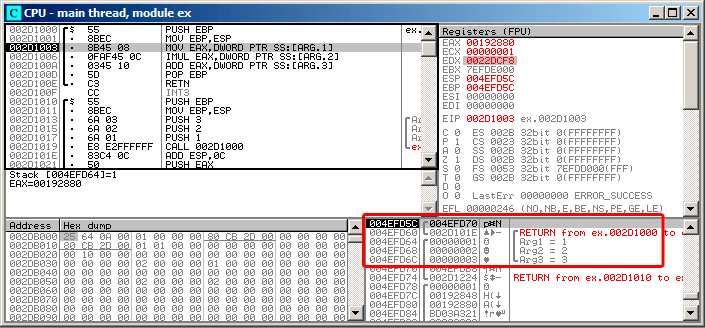
\includegraphics[scale=\FigScale]{patterns/05_passing_arguments/olly.png}
\caption{\olly: \RU{внутри ф-ции}\EN{inside of} \ttf{}\EN{ function}}
\label{fig:passing_arguments_olly}
\end{figure}
\fi

\subsection{GCC}

\RU{Скомпилируем то же в GCC 4.4.1 и посмотрим результат в \IDA:}
\EN{Let's compile the same in GCC 4.4.1 and let's see results in \IDA:}

\lstinputlisting[caption=GCC 4.4.1]{patterns/05_passing_arguments/gcc.asm}

\RU{Практически то же самое, если не считать мелких отличий описанных раннее.}
\EN{Almost the same result.}

\RU{После вызова обоих ф-ций, \glslink{stack pointer}{указатель стека} не возвращается назад, потому что предпоследняя
инструкция}\EN{The \gls{stack pointer} is not returning back after both function exeuction, because penultimate}
\TT{LEAVE} (\ref{x86_ins:LEAVE}) \RU{сделает это за один раз, в конце исполнения}\EN{instruction will do this,
at the end}.


\section{x64}

\index{x86-64}
\RU{В x86-64 всё немного иначе, здесь аргументы функции (4 или 6) передаются через регистры, 
а \gls{callee} из читает их из регистров, а не из стека.}
\EN{The story is a bit different in x86-64. Function arguments (first 4 or first 6 of them) 
are passed in registers i.e. the \gls{callee} reads them from registers instead of reading them from the stack.}

\subsection{MSVC}

\Optimizing MSVC:

\lstinputlisting[caption=\Optimizing MSVC 2012 x64]{patterns/05_passing_arguments/x64_MSVC_Ox.asm.\LANG}

\RU{Как видно, очень компактная функция \ttf берет аргументы прямо из регистров.}
\EN{As we can see, the compact function \ttf takes all its arguments from the registers.}
\RU{Инструкция \LEA используется здесь для сложения чисел. 
Должно быть компилятор посчитал, что это будет эффективнее использования \TT{ADD}.}
\EN{The \LEA instruction here is used for addition,
apparently the compiler considered it faster than \TT{ADD}.}
\index{x86!\Instructions!LEA}
\RU{В самой \main{} \LEA{} также используется для подготовки первого и третьего аргумента: должно быть,
компилятор решил, что \LEA{} будет работать здесь быстрее, чем загрузка значения в регистр при помощи \MOV.}
\EN{\LEA is also used in the \main function to prepare the first and third \ttf arguments. The compiler
must have decided that this would work faster than the usual way of loading values into a register using \MOV instruction.}

\RU{Попробуем посмотреть вывод неоптимизирующего MSVC}\EN{Let's take a look at the non-optimizing MSVC output}:

\lstinputlisting[caption=MSVC 2012 x64]{patterns/05_passing_arguments/x64_MSVC_IDA.asm.\LANG}

\RU{Немного путаннее: все 3 аргумента из регистров зачем-то сохраняются в стеке.}
\EN{It looks somewhat puzzling because all 3 arguments from the registers are saved to the stack for some reason.}
\index{Shadow space}
\label{shadow_space}
\RU{Это называется}\EN{This is called} ``shadow space''
\footnote{\href{http://go.yurichev.com/17256}{MSDN}}: 
\RU{каждая функция в Win64 может (хотя и не обязана) сохранять значения 4-х регистров там.}
\EN{every Win64 may (but is not required to) save all 4 register values there.}
\RU{Это делается по крайней мере из-за двух причин}\EN{This is done for two reasons}: 
1) \RU{в большой функции отвести целый регистр (а тем более 4 регистра) для входного аргумента 
слишком расточительно, так что к нему будет обращение через стек;}
\EN{it is too lavish to allocate a whole register (or even 4 registers) for an input argument,
so it will be accessed via stack;}
2) \RU{отладчик всегда знает, где найти аргументы функции в момент останова}\EN{the debugger is always
aware where to find the function arguments at a break}%
\footnote{\href{http://go.yurichev.com/17257}{MSDN}}.

\RU{Так что, какие-то большие функции могут сохранять входные аргументы в ``shadows space'' 
для использования в будущем, а небольшие функции, как наша, могут этого и не делать.}
\EN{So, some large functions can save their input arguments in the ``shadows space'' if they need to use them
during execution, but some small functions (like ours) may not do this.}

\RU{Место в стеке для ``shadow space'' выделяет именно \gls{caller}.}
\EN{It is a \gls{caller} responsibility to allocate ``shadow space'' in the stack.}

\ifdefined\IncludeGCC
\subsection{GCC}

\Optimizing GCC \RU{также делает понятный код}\EN{generates more or less understandable code}:

\lstinputlisting[caption=\Optimizing GCC 4.4.6 x64]{patterns/05_passing_arguments/x64_GCC_O3.s.\LANG}

\NonOptimizing GCC:

\lstinputlisting[caption=GCC 4.4.6 x64]{patterns/05_passing_arguments/x64_GCC.s.\LANG}

\index{Shadow space}
\RU{В соглашении о вызовах System V *NIX\cite{SysVABI} нет ``shadow space'', но \gls{callee} тоже иногда
должен сохранять где-то аргументы, потому что, опять же, регистров может и не хватить на все действия.
Что мы здесь и видим.}
\EN{There are no ``shadow space'' requirements in System V *NIX\cite{SysVABI}, but the \gls{callee} may need to save
its arguments somewhere in case of registers shortage.}

\subsection{GCC: uint64\_t \RU{вместо}\EN{instead of} int}

\RU{Наш пример работал с 32-битным \Tint, поэтому использовались 32-битные части регистров с префиксом \TT{E-}.}
\EN{Our example works with 32-bit \Tint, that is why 32-bit register parts are used (prefixed by \TT{E-}).}

\RU{Его можно немного переделать, чтобы он заработал с 64-битными значениями}\EN{It can be altered slightly
in order to use 64-bit values}:

\lstinputlisting{patterns/05_passing_arguments/ex64.c}

\lstinputlisting[caption=\Optimizing GCC 4.4.6 x64]{patterns/05_passing_arguments/ex64_GCC_O3_IDA.asm.\LANG}

\RU{Собствено, всё то же самое, только используются регистры \IT{целиком}, с префиксом \TT{R-}.}
\EN{The code is the same, but this time the \IT{full size} registers (prefixed by \TT{R-}) are used.}
\fi

\subsection{ARM}

\subsubsection{\NonOptimizingKeil + \ARMMode}

\begin{lstlisting}
.text:000000A4 00 30 A0 E1                 MOV     R3, R0
.text:000000A8 93 21 20 E0                 MLA     R0, R3, R1, R2
.text:000000AC 1E FF 2F E1                 BX      LR
...
.text:000000B0             main
.text:000000B0 10 40 2D E9                 STMFD   SP!, {R4,LR}
.text:000000B4 03 20 A0 E3                 MOV     R2, #3
.text:000000B8 02 10 A0 E3                 MOV     R1, #2
.text:000000BC 01 00 A0 E3                 MOV     R0, #1
.text:000000C0 F7 FF FF EB                 BL      f
.text:000000C4 00 40 A0 E1                 MOV     R4, R0
.text:000000C8 04 10 A0 E1                 MOV     R1, R4
.text:000000CC 5A 0F 8F E2                 ADR     R0, aD_0        ; "%d\n"
.text:000000D0 E3 18 00 EB                 BL      __2printf
.text:000000D4 00 00 A0 E3                 MOV     R0, #0
.text:000000D8 10 80 BD E8                 LDMFD   SP!, {R4,PC}
\end{lstlisting}

\IFRU{В функции \main просто вызываются две функции, в первую (\TT{f}) передается три значения.}
{In \main function, two other functions are simply called, and three values are passed to the 
first one (\TT{f}).}

\IFRU{Как я уже упоминал, первые 4 значения, в ARM обычно передаются в первых 4-х регистрах}
{As I mentioned before, in ARM, first 4 values are usually passed in first 4 registers} (\Rzero-\Rthree).

\IFRU{Функция }{}\TT{f}\IFRU{, как видно, использует три первых регистра (\Rzero-\Rtwo) как аргументы.}
{function, as it seems, use first 3 registers (\Rzero-\Rtwo) as arguments.}

\index{ARM!\Instructions!MLA}
\IFRU{Инструкция }{}\TT{MLA} (\IT{Multiply Accumulate}) \IFRU{перемножает два первых операнда (\Rthree и \Rone), 
прибавляет к произведению
третий операнд (\Rtwo) и помещает результат в нулевой операнд (\Rzero), через который, по стандарту, 
возвращаются значения функций.}
{instruction multiplicates two first operands (\Rthree and \Rone), adds third operand (\Rtwo) to product and places
result into zeroth operand (\Rzero), via which, by standard, values are returned from functions.}

\index{Fused multiply–add}
\IFRU{Умножение и сложение одновременно}{Multiplication and addition at once}\footnote{\WPMAO} 
(\IT{Fused multiply–add}) \IFRU{это много где применяемая операция, кстати, аналогичной
инструкции в x86 нет}{is very useful operation, by the way, there is no such instruction in x86}, 
\IFRU{если не считать новых FMA-инструкций}{if not to count new FMA-instruction}\footnote{\url{https://en.wikipedia.org/wiki/FMA_instruction_set}} \InENRU SIMD.

\IFRU{Самая первая инструкция}{The very first} \TT{MOV R3, R0}, \IFRU{по видимому, избыточна (можно было бы обойтись только одной инструкцией \TT{MLA})}
{instruction, apparently, redundant (single \TT{MLA} instruction could be used here instead)}, 
\IFRU{компилятор не оптимизировал её, ведь, это компиляция без оптимизации}{compiler was not optimized it,
since this is non-optimizing compilation}.

\index{ARM!\IFRU{Переключение режимов}{Mode switching}}
\index{ARM!\Instructions!BX}
\IFRU{Инструкция \TT{BX} возвращает управление по адресу записанному в \LR и, если нужно, 
переключает режимы процессора с thumb на ARM или наоборот.}
{\TT{BX} instruction returns control to the address stored in the \LR register and, if it is necessary, 
switches processor mode from thumb to ARM or vice versa.}
\IFRU{Это может быть необходимым потому, что, как мы видим, 
функции \TT{f} неизвестно, из какого кода она будет вызываться, из ARM или thumb.}
{This can be necessary since, as we can see, \TT{f} function is not aware, from which code it may be
called, from ARM or thumb.}
\IFRU{Поэтому, если она будет вызываться из кода thumb, \TT{BX} не только вернет
управление в вызывающую функцию, но также переключит процессор в режим thumb.}
{This, if it will be called from thumb code, \TT{BX} will not only return control to the calling function,
but also will switch processor mode to thumb mode.}
\IFRU{Либо не переключит, если функция вызывалась из кода для режима ARM.}
{Or not switch, if the function was called from ARM code.}

\subsubsection{\OptimizingKeil + \ARMMode}

\begin{lstlisting}
.text:00000098             f
.text:00000098 91 20 20 E0                 MLA     R0, R1, R0, R2
.text:0000009C 1E FF 2F E1                 BX      LR
\end{lstlisting}

\IFRU{А вот и функция \TT{f} скомпилированная компилятором Keil в режиме полной оптимизации}
{And here is \TT{f} function compiled by Keil compiler in full optimization mode} (\Othree).
\IFRU{Инструкция \MOV была соптимизирована и теперь \TT{MLA} использует все входящие регистры 
и помещает результат в \Rzero, как раз, где вызываемая функция будет его читать и использовать.}
{\MOV instruction was optimized (or reduced) and now \TT{MLA} uses all 
input registers and also places result right into \Rzero,
exactly where calling function will read it and use.}

\subsubsection{\OptimizingKeil + \ThumbMode}

\begin{lstlisting}
.text:0000005E 48 43                       MULS    R0, R1
.text:00000060 80 18                       ADDS    R0, R0, R2
.text:00000062 70 47                       BX      LR
\end{lstlisting}

\IFRU{В режиме thumb, инструкция \TT{MLA} недоступна, так что компилятору пришлось сгенерировать код, 
делающий обе операции по отдельности.}
{\TT{MLA} instruction is not available in thumb mode, so, compiler generates the code doing these two 
operations separately.}
\index{ARM!\Instructions!MULS}
\index{ARM!\Instructions!ADDS}
\IFRU{Первая инструкция \TT{MULS} умножает \Rzero на \Rone оставляя результат в \Rone.}
{First \TT{MULS} instruction multiply \Rzero by \Rone leaving result in the \Rone register.}
\IFRU{Вторая (\TT{ADDS}) складывает результат и \Rtwo, оставляя результат в \Rzero.}
{Second (\TT{ADDS}) instruction adds result and \Rtwo leaving result in the \Rzero register.}



\chapter{\RU{Еще о возвращаемых результатах}\EN{More about results returning}}

\index{x86!\Registers!EAX}
\RU{Результат выполнения функции в x86 обычно возвращается}
\EN{In x86, the result of function execution is usually returned}
\footnote{\Seealso: 
MSDN: Return Values (C++): \href{http://go.yurichev.com/17258}{MSDN}}
\RU{через регистр \EAX, 
а если результат имеет тип байт или символ (\Tchar), 
то в самой младшей части \EAX ~--- \AL. Если функция возвращает число с плавающей запятой, 
то будет использован регистр FPU \ST{0}.
\ifdefined\IncludeARM
\index{ARM!\Registers!R0}
В ARM обычно результат возвращается в регистре \Reg{0}.
\fi
}
\EN{in the \EAX register. 
If it is byte type or a character (\Tchar), then the lowest part of register \EAX (\AL) is used. 
If a function returns a \Tfloat number, the FPU register \ST{0} is used instead.
\ifdefined\IncludeARM
\index{ARM!\Registers!R0}
In ARM, the result is usually returned in the \Reg{0} register.
\fi
}

\section{\RU{Попытка использовать результат ф-ции возвращающей \Tvoid}
\EN{Attempt to use the result of a function returning \Tvoid}}

\RU{Кстати, что будет если возвращаемое значение в ф-ции \main объявлять не как \Tint а как \Tvoid?}
\EN{So, what if the \main function return value was declared of type \Tvoid and not \Tint?}

\RU{Т.н. startup-код вызывает \main примерно так:}
\EN{The so-called startup-code is calling \main roughly as follows:}

\begin{lstlisting}
push envp
push argv
push argc
call main
push eax
call exit
\end{lstlisting}

\RU{Т.е., иными словами:}\EN{In other words:}

\begin{lstlisting}
exit(main(argc,argv,envp));
\end{lstlisting}

\RU{Если вы объявите \main как \Tvoid, и ничего не будете возвращать явно (при помощи выражения \IT{return}), 
то в единственный аргумент exit() попадет
то, что лежало в регистре \EAX на момент выхода из \main.}
\EN{If you declare \main as \Tvoid, nothing will be returned explicitly (using the \IT{return} statement),
then something random, that was stored in the \EAX register at the end of \main will become 
the sole argument of the exit() function.}
\RU{Там, скорее всего, будет какие-то случайное число, оставшееся от работы вашей ф-ции.}
\EN{Most likely, there will be a random value, left from your function execution, }
\RU{Так что, код завершения программы будет псевдослучайным.}
\EN{so the exit code of program will be pseudorandom.} \\

\RU{Я могу это проиллюстрировать}\EN{I can illustrate this fact}. 
\RU{Заметьте что у ф-ции}\EN{Please note that here the} \main \RU{тип возвращаемого значения именно}\EN{function 
has a} \Tvoid\EN{ return type}:

\begin{lstlisting}
#include <stdio.h>

void main()
{
	printf ("Hello, world!\n");
};
\end{lstlisting}

\RU{Скомпилируем в}\EN{Let's compile it in} Linux.

\index{puts() \RU{вместо}\EN{instead of} printf()}
GCC 4.8.1 \RU{заменила}\EN{replaced} \printf \RU{на}\EN{with} \puts 
\ifx\LITE\undefined
(\RU{мы видели это прежде}\EN{we have seen this before}: \myref{puts})
\fi
, \RU{но это нормально, потому что}\EN{but that's OK, since} \puts \RU{возвращает количество
выведенных символов, так же как и}\EN{returns the number of characters printed out, just like} \printf.
\RU{Обратите внимание на то что}\EN{Please notice that} \EAX \RU{не обнуляется перед выходом их}\EN{is not 
zeroed before} \main\EN{'s end}.
\RU{Это значит,}\EN{This means that the value of} \EAX \RU{перед выходом из}\EN{at the end of} \main 
\RU{будет содержать то, что}\EN{will contain what} \puts \RU{оставит там}\EN{has left there}.

\begin{lstlisting}[caption=GCC 4.8.1]
.LC0:
	.string	"Hello, world!"
main:
	push	ebp
	mov	ebp, esp
	and	esp, -16
	sub	esp, 16
	mov	DWORD PTR [esp], OFFSET FLAT:.LC0
	call	puts
	leave
	ret
\end{lstlisting}

\index{bash}
\RU{Напишем небольшой скрипт на bash, показывающий статус возврата (``exit status'' или ``exit code'')}
\EN{Let' s write a bash script that shows the exit status}:

\begin{lstlisting}[caption=tst.sh]
#!/bin/sh
./hello_world
echo $?
\end{lstlisting}

\RU{И запустим}\EN{And run it}:

\begin{lstlisting}
$ tst.sh 
Hello, world!
14
\end{lstlisting}

$14$ \RU{это как раз количество выведенных символов}\EN{is the number of characters printed}.

\section{\RU{Что если не использовать результат ф-ции?}\EN{What if we do not use the function result?}}

\RU{\printf возвращает количество успешно выведенных символов, но результат работы этой ф-ции 
редко используется на практике.}
\EN{\printf returns the count of characters successfully output, but the result of this function 
is rarely used in practice.}
\RU{Можно даже явно вызывать ф-ции, чей смысл именно в возвращаемых значениях, но явно не использовать их:}
\EN{It is also possible to call a function whose essence is in returning a value, and not use it:}

\begin{lstlisting}
int f()
{
    // skip first 3 random values
    rand();
    rand();
    rand();
    // and use 4th
    return rand();
};
\end{lstlisting}

\EN{The result of the rand() function will always be left in \EAX, in all four cases.}
\RU{Результат работы rand() будет оставаться в \EAX во всех четырех случаях.}
\EN{But in the first 3 cases, the value in \EAX will be just thrown away.}
\RU{Но в первых трех случаях, значение лежащее в \EAX, будет просто выброшено.}

\ifx\LITE\undefined
\section{\RU{Возврат структуры}\EN{Returning a structure}}

\index{\CLanguageElements!return}
\RU{Вернемся к тому факту, что возвращаемое значение остается в регистре \EAX}
\EN{Let's go back to the fact that the return value is left in the \EAX register}.
\RU{Вот почему старые компиляторы Си не способны создавать функции, возвращающие нечто большее, нежели 
помещается 
в один регистр (обычно, тип \Tint), а когда нужно, приходится возвращать через указатели, указываемые 
в аргументах.}
\EN{That is why old C compilers cannot create functions capable of returning something that does not fit in one 
register (usually \Tint), but if one needs it, one have to return information via pointers passed 
as function's arguments.}
\RU{Так что, как правило, если ф-ция должна вернуть несколько значений, она возвращает только одно, 
а остальные --- через указатели.}
\EN{So, usually, if a function needs to return several values, it returns only one, and 
all the rest---via pointers.}
\RU{Хотя, позже и стало возможным, вернуть, скажем, целую структуру, но этот метод до сих пор не 
очень популярен. 
Если функция должна вернуть структуру, вызывающая функция должна сама, скрыто и прозрачно для программиста, 
выделить место и передать указатель на него в качестве первого аргумента. Это почти то же самое 
что и сделать это вручную, но компилятор прячет это.}
\EN{Now it has become possible to return, let's say, an entire structure, but that is still not very popular. 
If a function has to return a large structure, the \gls{caller} must allocate it and pass a pointer to it via the first argument, transparently for the programmer. 
That is almost the same as to pass a pointer in the first argument manually, but the compiler hides it.}

\RU{Небольшой пример:}\EN{Small example:}

\lstinputlisting{patterns/06_return_results/6_1.c}

\dots \RU{получим}\EN{what we got} (MSVC 2010 \Ox):

\lstinputlisting{patterns/06_return_results/6_1.asm}

\RU{Имя внутреннего макроса для передачи указателя на структуру здесь это \TT{\$T3853}.}
\EN{The macro name for internal passing of pointer to a structure her is \TT{\$T3853}.}

\index{\CLanguageElements!C99}
\RU{Этот пример можно даже переписать, используя расширения C99}\EN{This example can be rewritten using
the C99 language extensions}:

\lstinputlisting{patterns/06_return_results/6_1_C99.c}

\lstinputlisting[caption=GCC 4.8.1]{patterns/06_return_results/6_1_C99.asm}

\RU{Как видно, ф-ция просто заполняет поля в структуре, выделенной вызывающей ф-цией. 
Как если бы передавался просто указатель на структуру.
Так что никаких проблем с эффективностью нет.}
\EN{As we see, the function is just filling the structure's fields allocated by
the caller function,
as if a pointer to the structure was passed.
So there are no performance drawbacks.}
\fi

\ifx\LITE\undefined
\section{\IFRU{Указатели}{Pointers}}
\index{\CLanguageElements!\Pointers}
\label{label_pointers}

\newcommand{\ttf}{\TT{f1()}}

\IFRU{Указатели также часто используются для возврата значений из функции (вспомните случай
со \scanf{}~(\ref{label_scanf}))}
{Pointers are often used to return values from function (recall \scanf case~(\ref{label_scanf}))}.
\IFRU{Например, когда функции нужно вернуть сразу два значения}
{For example, when function should return two values}.

\subsection{\IFRU{Пример с глобальными переменными}{Global variables example}}

\lstinputlisting{patterns/061_pointers/global.c}

\IFRU{Это компилируется в}{This compiling into}:

\lstinputlisting[caption=\Optimizing MSVC 2010 (/Ox /Ob0)]{patterns/061_pointers/global.asm}

\index{\olly}
\IFRU{Посмотрим это в}{Let's see this in} \olly: \figname \ref{fig:pointers_olly_global_1}.
\IFRU{В начале адреса обоих глобальных переменных передаются в}{At first, global
variables addresses are passed into} \ttf.
\IFRU{Можно нажать}{We can click} ``Follow in dump'' \IFRU{на элементе стека и в окне слева 
увидим место в сегменте данных выделенных для двух переменных}{on the stack element, and we will see 
a place in data segment allocated for two variables}.
\IFRU{Эти переменные обнулены, потому что, по стандарту, неинициализированные данные (\ac{BSS}) 
обнуляются перед началом исполнения}
{These variables are cleared, because non-initialized data (\ac{BSS}) are cleared before
execution begin}.
\IFRU{И они находятся в сегменте данных, о чем можно удостовериться нажав}
{They are residing in data segment, we can be sure it is so, by pressing} Alt-M \IFRU{и увидев карту
памяти}{and seeing memory map}: \figname \ref{fig:pointers_olly_global_5}.

\IFRU{Трассируем}{Let's trace} (F7) \IFRU{до начала исполнения}{until execution of} \ttf 
\figname \ref{fig:pointers_olly_global_2}.
\IFRU{В стеке видны и значения}{Two values are seen in the stack} $456$ (\TT{0x1C8}) \AndENRU 
$123$ (\TT{0x7B}), \IFRU{а также адреса двух глобальных переменных}{and two global variables addresses
as well}.

\IFRU{Трассируем до конца}{Let's trace until the end of} \ttf.
\IFRU{Мы видим в окне слева, как результаты вычисления появились в глобальных переменных}
{At the window at left we see how calculation results are appeared in the gloval variables} 
\figname \ref{fig:pointers_olly_global_3}.

\IFRU{Теперь из глобальных переменных значения загружаются в регистры для передачи в}
{Now values of global variables are loaded into registers for passing into} \printf:
\figname \ref{fig:pointers_olly_global_4}.

\begin{figure}[H]
\centering
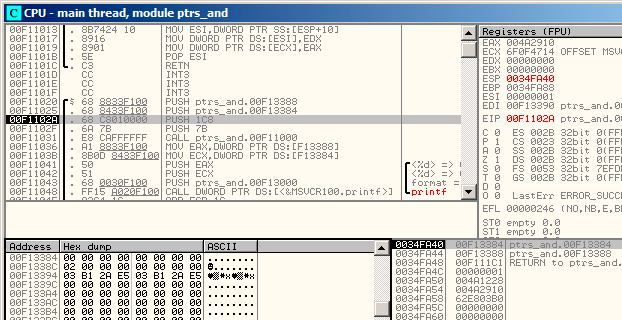
\includegraphics[scale=0.66]{patterns/061_pointers/olly_global1.png}
\caption{\olly: \IFRU{передаются адреса двух глобальных переменных в}
{global variables addresses are passing into} \ttf}
\label{fig:pointers_olly_global_1}
\end{figure}

\begin{figure}[H]
\centering
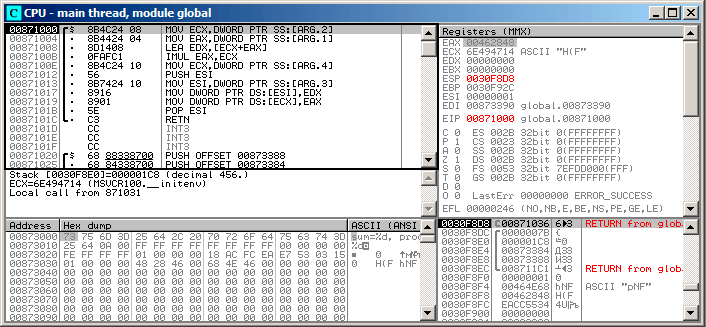
\includegraphics[scale=0.66]{patterns/061_pointers/olly_global2.png}
\caption{\olly: \IFRU{начало работы \ttf}{\ttf is started}}
\label{fig:pointers_olly_global_2}
\end{figure}

\begin{figure}[H]
\centering
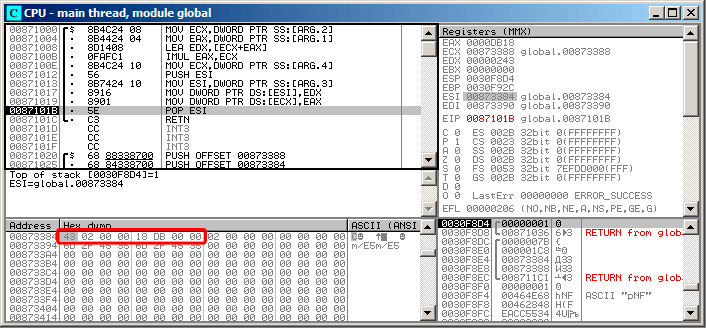
\includegraphics[scale=0.66]{patterns/061_pointers/olly_global3.png}
\caption{\olly: \ttf \IFRU{заканчивает работу}{finishes}}
\label{fig:pointers_olly_global_3}
\end{figure}

\begin{figure}[H]
\centering
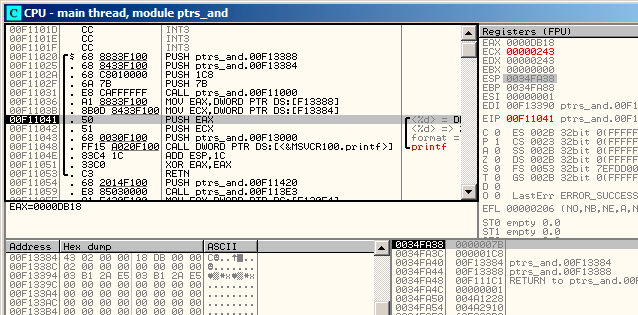
\includegraphics[scale=0.66]{patterns/061_pointers/olly_global4.png}
\caption{\olly: \IFRU{адреса глобальных переменных передаются в}
{global variables addresses are passed into} \printf}
\label{fig:pointers_olly_global_4}
\end{figure}

\begin{figure}[H]
\centering
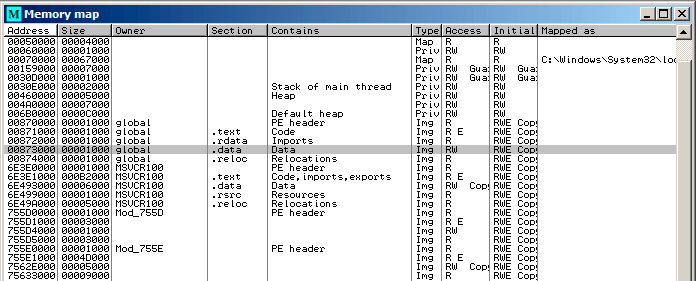
\includegraphics[scale=0.66]{patterns/061_pointers/olly_global5.png}
\caption{\olly: \IFRU{карта памяти}{memory map}}
\label{fig:pointers_olly_global_5}
\end{figure}

\subsection{\IFRU{Пример с локальными переменными}{Local variables example}}

\IFRU{Немного переделаем пример}{Let's rework our example slightly}:

\lstinputlisting[caption=\IFRU{теперь переменные локальные}
{now variables are local}]{patterns/061_pointers/local_\IFRU{ru}{en}.c}

\RU{Код ф-ции }\ttf \IFRU{не изменится}{function code will not changed}.
\IFRU{Изменится только \main}{Only \main code will}:

\lstinputlisting[caption=\Optimizing MSVC 2010 (/Ox /Ob0)]{patterns/061_pointers/local.asm}

\newcommand{\PtrsAddresses}{\TT{0x35FCF4} \AndENRU \TT{0x35FCF8}\xspace}

\IFRU{Снова посмотрим в}{Let's again take a look into} \olly.
\IFRU{Адреса локальных переменных в стеке это}{Local variable addresses in the stack are} \PtrsAddresses.
\IFRU{Видно как они заталкиваются в стек}{We see how these are pushed into the stack}: 
\figname \ref{fig:pointers_olly_stk_1}.

\IFRU{Начало работы \ttf}{\ttf is started}.
\IFRU{В стеке по адресам}{Random garbage are at} \PtrsAddresses \IFRU{пока находится случайный мусор}
{so far} \figname \ref{fig:pointers_olly_stk_2}.

\IFRU{Конец работы \ttf}{\ttf finished}.
\IFRU{В стеке по адресам \PtrsAddresses теперь значения \TT{0xDB18} \AndENRU \TT{0x243}, 
это результаты работы \ttf}
{There are \TT{0xDB18} \AndENRU \TT{0x243} now at \PtrsAddresses addresses, these values are
\ttf function result}.

\begin{figure}[H]
\centering
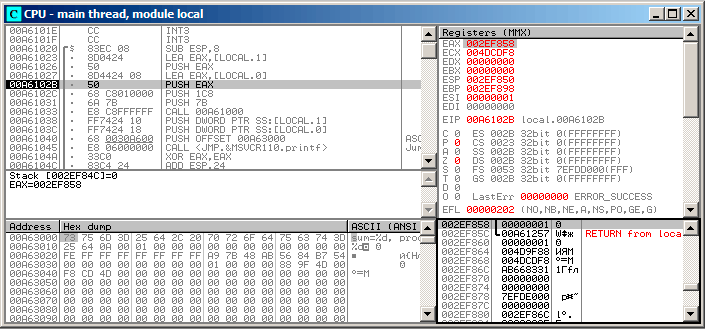
\includegraphics[scale=0.66]{patterns/061_pointers/olly_stk1.png}
\caption{\olly: \IFRU{адреса локальных переменных заталкиваются в стек}{addresses of local variables are
pushed into the stack}}
\label{fig:pointers_olly_stk_1}
\end{figure}

\begin{figure}[H]
\centering
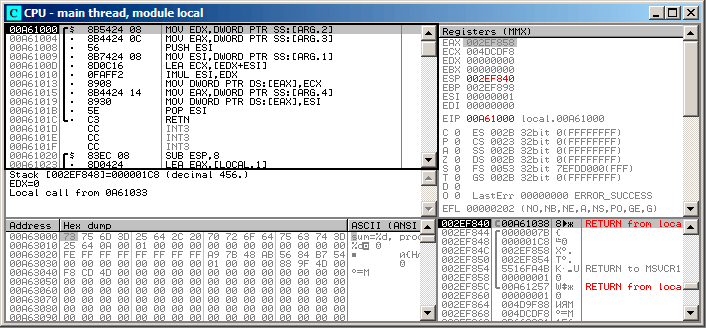
\includegraphics[scale=0.66]{patterns/061_pointers/olly_stk2.png}
\caption{\olly: \ttf \IFRU{начинает работу}{starting}}
\label{fig:pointers_olly_stk_2}
\end{figure}

\begin{figure}[H]
\centering
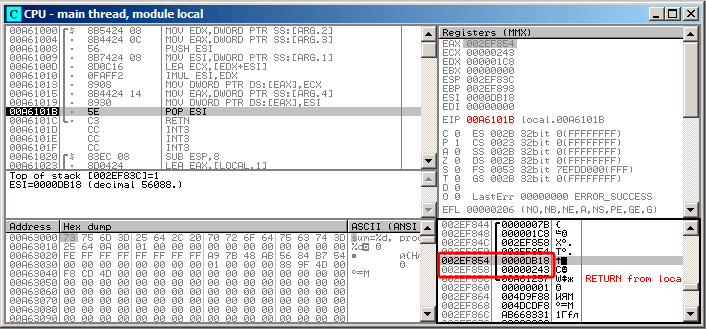
\includegraphics[scale=0.66]{patterns/061_pointers/olly_stk3.png}
\caption{\olly: \ttf \IFRU{заканчивает работу}{finished}}
\label{fig:pointers_olly_stk_3}
\end{figure}

\subsection{\IFRU{Вывод}{Conclusion}}

\IFRU{\ttf может одинаково хорошо возвращать результаты работы в любые места памяти, 
находящиеся где угодно}{\ttf can return results to any place in memory, located anywhere}.
\IFRU{В этом суть и удобство указателей}{This is essence and usefulness of pointers}.

\IFRU{Кстати,}{By the way, \Cpp} \IT{references} \IFRU{в \Cpp работают точно так же}{works just in the
same way}. \IFRU{Читайте больше об этом}{Read more about them}: (\ref{cpp_references}).


\fi
\chapter{GOTO}

\RU{Оператор GOTO считается анти-паттерном}\EN{GOTO operator considered harmful} 
\cite{Dijkstra:1968:LEG:362929.362947}, 
\RU{но тем не менее, его можно использовать в разумных пределах}
\EN{but nevertheless, can be used resonably} \cite{Knuth:1974:SPG:356635.356640}, \cite[1.3.2]{CBook}.

\RU{Вот простейший пример}\EN{Here is a simplest possible example}:

\lstinputlisting{patterns/065_GOTO/goto.c}

\RU{Вот что мы получаем в}\EN{Here is what we've got is} MSVC 2012:

\lstinputlisting[caption=MSVC 2012]{patterns/065_GOTO/MSVC_goto.asm}

\RU{Так что выражение \IT{goto} просто заменяется инструкцией \JMP, которая работает точно также:
безусловный переход в другое место.}
\EN{So the \IT{goto} statement is just replaced by \JMP instruction, which has the very same
effect: unconditional jump to another place.}

\RU{Вызов второго \printf может исполнится только при помощи человеческого вмешательства,
используя отладчик или модифицирование кода.}
\EN{The second \printf call can be executed only with the help of human intervention, 
using debugger or patching.}\\
\\
\RU{Это также может быть простым упражнением на модификацию кода.}
\EN{This also could be a simple patching exercise.}
\RU{Откроем исполняемый файл в}\EN{Let's open resulting executable in} Hiew: \figref{fig:goto_hiew1}.

\RU{Поместите курсор по адресу где}\EN{Place cursor to the address of} \JMP (\TT{0x410}), 
\RU{нажмите}\EN{press} F3 (\RU{редактирование}\EN{edit}), \RU{нажмите два нуля, так что
опкод будет}\EN{press two zeroes, so the opcode will be} \TT{EB 00}: \figref{fig:goto_hiew2}.

\RU{Второй байт опкода \JMP означает относительное смещение от перехода, 0 означает место
прямо после текущей инструкции.}
\EN{The second byte of \JMP opcode mean relative offset of jump, 0 means the point
right after current instruction.}
\RU{Теперь \JMP не будет пропускать следующий вызов \printf.}
\EN{So now \JMP will not skip second \printf call.}

\RU{Теперь нажмите F9 (запись) и выйдите.}
\EN{Now press F9 (save) and exit.}
\RU{Теперь мы запускаем исполняемый файл и видим это}\EN{Now we run executable and we see 
this}: \figref{fig:goto_result}.

\RU{Подобного же эффекта можно достичь, если заменить инструкцию \JMP на две инструкции \NOP.}
\EN{The same effect can be achieved if to replace \JMP instruction by 2 \NOP instructions.}
\RU{\NOP имеет опкод \TT{0x90} и длину в 1 байт, так что нужно 2 инструкции для замены.}
\EN{\NOP has \TT{0x90} opcode and length of 1 byte, so we need 2 instructions as replacement.}

\begin{figure}[H]
\centering
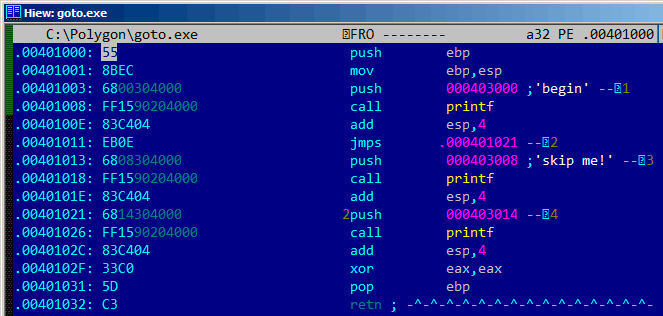
\includegraphics[scale=0.66]{patterns/065_GOTO/hiew1.png}
\caption{Hiew}
\label{fig:goto_hiew1}
\end{figure}

\begin{figure}[H]
\centering
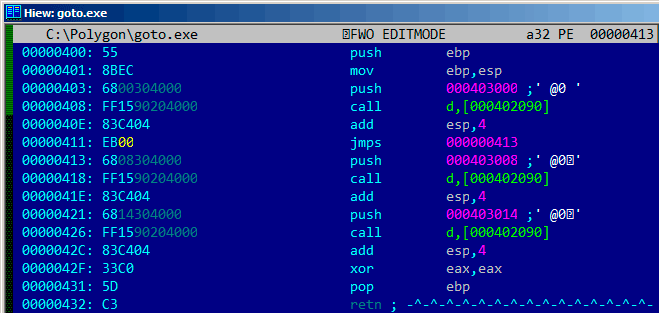
\includegraphics[scale=0.66]{patterns/065_GOTO/hiew2.png}
\caption{Hiew}
\label{fig:goto_hiew2}
\end{figure}

\begin{figure}[H]
\centering
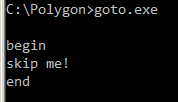
\includegraphics[scale=0.66]{patterns/065_GOTO/result.png}
\caption{\RU{Результат}\EN{Result}}
\label{fig:goto_result}
\end{figure}

\section{\RU{Мертвый код}\EN{Dead code}}

\RU{Вызов второго \printf также называется ``мертвым кодом'' (``dead code'') 
в терминах компиляторов.}
\EN{The second \printf call is also called ``dead code'' in compiler's term.}
\RU{Это значит что он никогда не будет исполнен}\EN{This mean, the code will never be executed}.
\EN{So when you compile this example with optimization, compiler removing ``dead code'' leaving
no trace of it:}
\RU{Так что если вы компилируете этот пример с оптимизацией, компилятор удаляет ``мертвый
код'' не оставляя следа:}

\lstinputlisting[caption=\Optimizing MSVC 2012]{patterns/065_GOTO/MSVC_goto_Ox.asm}

\RU{Впрочем, строку}\EN{However, compiler forgot to remove the} ``skip me!'' \RU{компилятор 
убрать забыл}\EN{string}.

\section{\Exercise}

\RU{Попробуйте добиться того же самого используя ваш любимый компилятор и отладчик.}
\EN{Try to achieve the same result using your favorite compiler and debugger.}

\chapter{\RU{Условные переходы}\EN{Conditional jumps}}
\label{sec:Jcc}
\index{\CLanguageElements!if}

% sections
\section{\RU{Простой пример}\EN{Simple example}}

\lstinputlisting{patterns/07_jcc/simple/ex.c}

% subsections
\input{patterns/07_jcc/simple/x86}
\input{patterns/07_jcc/simple/ARM/main}
\EN{\input{patterns/07_jcc/simple/MIPS_EN}}
\RU{\input{patterns/07_jcc/simple/MIPS_RU}}

\section{\RU{Вычисление абсолютной величины}\EN{Calculating absolute value}}
\label{sec:abs}

\RU{Это простая функция}\EN{A simple function}:

\lstinputlisting{abs.c}

\subsection{\Optimizing MSVC}

\RU{Обычный способ генерации кода:}
\EN{This is how the code is usually generated:}

\lstinputlisting[caption=\Optimizing MSVC 2012 x64]{patterns/07_jcc/abs/abs_MSVC2012_Ox_x64.asm.\LANG}

\ifdefined\IncludeGCC
\RU{GCC 4.9 делает почти то же самое.}
\EN{GCC 4.9 does mostly the same.}
\fi

\ifdefined\IncludeARM
\subsection{\OptimizingKeilVI: \ThumbMode}

\lstinputlisting[caption=\OptimizingKeilVI: \ThumbMode]{patterns/07_jcc/abs/abs_Keil_thumb_O3.s.\LANG}

\myindex{ARM!\Instructions!RSB}
\RU{В ARM нет инструкции для изменения знака, так что компилятор Keil использует инструкцию \q{Reverse Subtract},
которая просто вычитает, но с операндами, переставленными наоборот.}
\EN{ARM lacks a negate instruction, so the Keil compiler uses the \q{Reverse Subtract} instruction, which just subtracts with reversed operands.}

\subsection{\OptimizingKeilVI: \ARMMode}

\RU{В режиме ARM можно добавлять коды условий к некоторым инструкций, что компилятор Keil и сделал:}
\EN{It is possible to add condition codes to some instructions in ARM mode, so that is what the Keil compiler does:}

\lstinputlisting[caption=\OptimizingKeilVI: \ARMMode]{patterns/07_jcc/abs/abs_Keil_ARM_O3.s.\LANG}

\RU{Теперь здесь нет условных переходов и это хорошо:}
\EN{Now there are no conditional jumps and this is good:} 
\myref{branch_predictors}.

\subsection{\NonOptimizing GCC 4.9 (ARM64)}

\myindex{ARM!\Instructions!XOR}
\RU{В ARM64 есть инструкция NEG для смены знака:}
\EN{ARM64 has instruction NEG for negating:}

\lstinputlisting[caption=\Optimizing GCC 4.9 (ARM64)]{patterns/07_jcc/abs/abs_GCC49_ARM64_O0.s.\LANG}
\fi

\ifdefined\IncludeMIPS
\subsection{MIPS}

\lstinputlisting[caption=\Optimizing GCC 4.4.5 (IDA)]{patterns/07_jcc/abs/MIPS_O3_IDA.lst.\LANG}

\myindex{MIPS!\Instructions!BLTZ}
\RU{Видим здесь новую инструкцию}\EN{Here we see a new instruction}: BLTZ (\q{Branch if Less Than Zero}).
\myindex{MIPS!\Instructions!SUBU}
\myindex{MIPS!\Pseudoinstructions!NEGU}
\RU{Тут есть также псевдоинструкция NEGU, которая на самом деле вычитает из нуля.}
\EN{There is also the NEGU pseudoinstruction, which just does subtraction from zero.}
\RU{Суффикс \q{U} в обоих инструкциях SUBU и NEGU означает, что при целочисленном переполнении исключение не
сработает.}
\EN{The \q{U} suffix in both SUBU and NEGU implies that no exception to be raised in case of integer overflow.}

\fi

\subsection{\RU{Версия без переходов}\EN{Branchless version}?}

\RU{Возможна также версия и без переходов, мы рассмотрим её позже:}
\EN{You could have also a branchless version of this code. This we will review later:} \myref{chap:branchless_abs}.

\section{\RU{Условный оператор}\EN{Conditional operator}}
\label{chap:cond}

\RU{Условный оператор (conditional operator) в}\EN{Conditional operator in} \CCpp \RU{это}\EN{is}:

\begin{lstlisting}
expression ? expression : expression
\end{lstlisting}

\RU{И вот пример}\EN{Now here is an example}:

\lstinputlisting{patterns/07_jcc/cond_operator/cond.c}

\subsection{x86}

\RU{Старые и неоптимизирующие компиляторы генерируют код так, как если бы выражение \TT{if/else} было использовано
вместо:}
\RU{Old and non-optimizing compilers generate the code just as if \TT{if/else} statmement was used instead:}

\lstinputlisting[caption=\NonOptimizing MSVC 2008]{patterns/07_jcc/cond_operator/MSVC2008.asm}

\lstinputlisting[caption=\Optimizing MSVC 2008]{patterns/07_jcc/cond_operator/MSVC2008_Ox.asm}

\RU{Более новые компиляторы могут быть более краткими}\EN{Latest compilers may be more concise}:

\lstinputlisting[caption=\Optimizing MSVC 2012 x64]{patterns/07_jcc/cond_operator/MSVC2012_Ox_x64.asm}

\index{x86!\Instructions!CMOVcc}
\Optimizing GCC 4.8 \ForENRU x86 \RU{также использует инструкцию}\EN{also use} \TT{CMOVcc}\RU{, тогда как
неоптимизирующий GCC 4.8 использует условные переходы}\EN{ instruction, while non-optimizing GCC 4.8 use 
conditional jumps}.

\subsection{ARM}

\index{x86!\Instructions!ADRcc}
\Optimizing Keil \ForENRU \RU{режима ARM также использует инструкцию \TT{ADRcc}, срабатывающую при некотором
условии}\EN{ARM mode also use conditional instructions \TT{ADRcc}}:

\lstinputlisting[label=cond_Keil_ARM_O3,caption=\OptimizingKeilVI (\ARMMode)]{patterns/07_jcc/cond_operator/Keil_ARM_O3.s}

\RU{Без внешнего вмешательства, инструкции \TT{ADREQ} и \TT{ADRNE} никогда не исполнятся одновременно.}
\EN{Without manual intervention, both \TT{ADREQ} and \TT{ADRNE} instructions cannot be executed.}

\Optimizing Keil \ForENRU \RU{режима Thumb вынужден использовать инструкции условного перехода, потому
что тут нет инструкции загрузки значения поддерживающую флаги условия}\EN{Thumb mode ought to use 
conditional jump instructions, since there are no load instruction
supporting conditional flags}:

\lstinputlisting[caption=\OptimizingKeilVI (\ThumbMode)]{patterns/07_jcc/cond_operator/Keil_thumb_O3.s}

\subsection{ARM64}

\Optimizing GCC (Linaro) 4.9 \ForENRU ARM64 \RU{также использует условные переходы}\EN{also use conditional jumps}:

\lstinputlisting[label=cond_ARM64,caption=\Optimizing GCC (Linaro) 4.9]{patterns/07_jcc/cond_operator/ARM64_GCC_O3.s}

\RU{Это потому что в ARM64 нет простой инструкции загрузки с флагами условия, как \TT{ADRcc} в 32-битном 
режиме ARM или \TT{CMOVcc} в x86}
\EN{That's because ARM64 hasn't simple load instruction with conditional flags, like \TT{ADRcc} in 32-bit 
ARM mode or CMOVcc in x86}
\cite[p390, C5.5]{ARM64ref}.
\index{ARM!\Instructions!CSEL}
\RU{Но с другой стороны, там есть инструкция \TT{CSEL} (``Conditional SELect''), но GCC 4.9 наверное пока не так
хорош, чтобы генерировать её в таком фрагменте кода.}
\EN{It has, however, ``Conditional SELect'' instruction (\TT{CSEL}), but GCC 4.9 is probably not that good to 
generate it in such piece of code.}

\subsection{\RU{Перепишем используя обычный \TT{if/else}}\EN{Let's rewrite it in \TT{if/else} way}}

\lstinputlisting{patterns/07_jcc/cond_operator/cond2.c}

\index{x86!\Instructions!CMOVcc}
\RU{Интересно, оптимизирующий GCC 4.8 для x86 также может генерировать \TT{CMOVcc} в этом случае:}
\EN{Interestingly, optimizing GCC 4.8 for x86 also was able to generate \TT{CMOVcc} in this case:}

\lstinputlisting[caption=\Optimizing GCC 4.8]{patterns/07_jcc/cond_operator/cond2_GCC_O3.s}

\Optimizing Keil \InENRU \RU{режиме ARM генерирует код идентичный этому:}\EN{ARM mode generates a 
code identical to} \lstref{cond_Keil_ARM_O3}.

\RU{Но оптимизирующий}\EN{But optimizing} MSVC 2012 \RU{пока не так хорош}\EN{is not that good (yet)}.

\subsection{\Conclusion{}}

\RU{Почему оптимизирующие компиляторы стараются избавиться от условных переходов? Читайте больше об этом здесь:}
\EN{Why optimizing compilers try to get rid of conditional jumps? Read here about it:} \ref{branch_predictors}.

\subsection{\Exercise}

\RU{Попробуйте переписать код в}\EN{Try to rewrite the code in} \lstref{cond_ARM64} 
\RU{убрав все инструкции условного перехода, и используйте инструкцию \TT{CSEL}}\EN{by removing all 
conditional jump instructions, and use \TT{CSEL} instruction}.

\section{\RU{Поиск минимального и максимального значения}\EN{Getting minimal and maximal values}}

\subsection{32-bit}

\lstinputlisting{patterns/07_jcc/minmax/minmax.c}

\lstinputlisting[caption=\NonOptimizing MSVC 2013]{patterns/07_jcc/minmax/minmax_MSVC_2013.asm.\LANG}

\myindex{x86!\Instructions!Jcc}
\RU{Эти две функции отличаются друг от друга только инструкцией условного перехода:
JGE (\q{Jump if Greater or Equal}~--- переход если больше или равно) используется в первой
и JLE (\q{Jump if Less or Equal}~--- переход если меньше или равно) во второй.}
\EN{These two functions differ only in the conditional jump instruction: 
JGE (\q{Jump if Greater or Equal}) is used in the first one
and JLE (\q{Jump if Less or Equal}) in the second.}

\myindex{\CompilerAnomaly}
\label{MSVC_double_JMP_anomaly}
\RU{Здесь есть ненужная инструкция \JMP в каждой функции, которую MSVC, наверное, оставил по ошибке.}
\EN{There is one unneeded \JMP instruction in each function, which MSVC probably left by mistake.}

\subsubsection{\RU{Без переходов}\EN{Branchless}}

\RU{ARM в режиме Thumb напоминает нам x86-код:}
\EN{ARM for Thumb mode reminds us of x86 code:}

\lstinputlisting[caption=\OptimizingKeilVI (\ThumbMode)]{patterns/07_jcc/minmax/minmax_Keil_Thumb_O3.s.\LANG}

\myindex{ARM!\Instructions!Bcc}
\RU{Функции отличаются только инструкцией перехода: BGT и BLT.}
\EN{The functions differ in the branching instruction: BGT and BLT.}

\RU{А в режиме ARM можно использовать условные суффиксы, так что код более плотный.}
\EN{It's possible to use conditional suffixes in ARM mode, so the code is shorter.}
\RU{MOVcc будет исполнена только если условие верно:}
\EN{MOVcc is to be executed only if the condition is met:}
\myindex{ARM!\Instructions!MOVcc}

\lstinputlisting[caption=\OptimizingKeilVI (\ARMMode)]{patterns/07_jcc/minmax/minmax_Keil_ARM_O3.s.\LANG}

\myindex{x86!\Instructions!CMOVcc}
\Optimizing GCC 4.8.1 \RU{и оптимизирующий}\EN{and optimizing} MSVC 2013 
\RU{могут использовать инструкцию CMOVcc, которая аналогична MOVcc в ARM:}
\EN{can use CMOVcc instruction, which is analogous to MOVcc in ARM:}

\lstinputlisting[caption=\Optimizing MSVC 2013]{patterns/07_jcc/minmax/minmax_GCC481_O3.s.\LANG}

\subsection{64-bit}

\lstinputlisting{patterns/07_jcc/minmax/minmax64.c}

\RU{Тут есть ненужные перетасовки значений, но код в целом понятен:}
\EN{There is some unneeded value shuffling, but the code is comprehensible:}

\lstinputlisting[caption=\NonOptimizing GCC 4.9.1 ARM64]{patterns/07_jcc/minmax/minmax64_GCC_49_ARM64_O0.s}

\subsubsection{\RU{Без переходов}\EN{Branchless}}

\RU{Нет нужды загружать аргументы функции из стека, они уже в регистрах:}
\EN{No need to load function arguments from the stack, as they are already in the registers:}

\lstinputlisting[caption=\Optimizing GCC 4.9.1 x64]{patterns/07_jcc/minmax/minmax64_GCC_49_x64_O3.s.\LANG}

MSVC 2013 \RU{делает то же самое}\EN{does almost the same}.

\myindex{ARM!\Instructions!CSEL}
\RU{В ARM64 есть инструкция CSEL, которая работает точно также, как и MOVcc в ARM и CMOVcc в x86, но название
другое:}
\EN{ARM64 has the CSEL instruction, which works just as MOVcc in ARM or CMOVcc in x86, just the name is different:}
\q{Conditional SELect}.

\lstinputlisting[caption=\Optimizing GCC 4.9.1 ARM64]{patterns/07_jcc/minmax/minmax64_GCC_49_ARM64_O3.s.\LANG}

\ifdefined\IncludeMIPS
\subsection{MIPS}

\RU{А GCC 4.4.5 для MIPS не так хорош, к сожалению}\EN{Unfortunately, GCC 4.4.5 for MIPS is not that good}:

\lstinputlisting[caption=\Optimizing GCC 4.4.5 (IDA)]{patterns/07_jcc/minmax/minmax_MIPS_O3_IDA.lst.\LANG}

\RU{Не забывайте о \IT{branch delay slots}: первая MOVE исполняется \IT{перед} BEQZ,
вторая MOVE исполняется только если переход не произошел.}
\EN{Do not forget about the \IT{branch delay slots}: the first MOVE is executed \IT{before} BEQZ, 
the second MOVE is executed only if the branch wasn't taken.}

\fi % MIPS



\section{\Conclusion{}}

\subsection{x86}

\RU{Примерный скелет условных переходов}\EN{Here's the rough skeleton of a conditional jump}:

\lstinputlisting[caption=x86]{patterns/07_jcc/skel1.lst.\LANG}

\ifdefined\IncludeARM

\subsection{ARM}

\lstinputlisting[caption=ARM]{patterns/07_jcc/skel2.lst.\LANG}
\fi

\ifdefined\IncludeMIPS

\subsection{MIPS}

\begin{lstlisting}[caption=\RU{Проверка на ноль}\EN{Check for zero}]
BEQZ REG, label
...
\end{lstlisting}

\begin{lstlisting}[caption=\RU{Меньше ли нуля?}\EN{Check for less than zero:}]
BLTZ REG, label
...
\end{lstlisting}

\begin{lstlisting}[caption=\RU{Проверка на равенство}\EN{Check for equal values}]
BEQ REG1, REG2, label
...
\end{lstlisting}

\begin{lstlisting}[caption=\RU{Проверка на неравенство}\EN{Check for non-equal values}]
BNE REG1, REG2, label
...
\end{lstlisting}

\begin{lstlisting}[caption=\RU{Проверка на меньше, больше (знаковое)}\EN{Check for less than, greater than (signed)}]
SLT REG1, REG2, REG3
BEQ REG1, label
...
\end{lstlisting}

\begin{lstlisting}[caption=\RU{Проверка на меньше, больше (беззнаковое)}\EN{Check for less than, greater than (unsigned)}]
SLTU REG1, REG2, REG3
BEQ REG1, label
...
\end{lstlisting}
\fi

\subsection{\RU{Без инструкций перехода}\EN{Branchless}}

\index{ARM!\Instructions!MOVcc}
\index{x86!\Instructions!CMOVcc}
\index{ARM!\Instructions!CSEL}
\EN{If the body of a condition statement is very short, the conditional move instruction can be used: 
MOVcc in ARM (in ARM mode), CSEL in ARM64, CMOVcc in x86.}
\RU{Если тело условного выражения очень короткое, инструкция условного копирования может быть
использована: MOVcc в ARM (в режиме ARM), CSEL в ARM64, CMOVcc в x86.}

\ifdefined\IncludeARM
\subsubsection{ARM}

\RU{В режиме ARM, Можно использовать условные суффиксы для некоторых инструкций:}
\EN{It's possible to use conditional suffixes in ARM mode for some instructions:}

\lstinputlisting[caption=ARM (\ARMMode)]{patterns/07_jcc/skel4.lst.\LANG}

\RU{Конечно, нет никаких ограничений на количество инструкций с условными суффиксами, до тех пор
пока флаги CPU не были модифицированы одной из таких инструкций.}
\EN{Of course, there is no limit for the number of instructions with conditional code suffixes, 
as long as the CPU flags are not modified by any of them.}
% FIXME: list of such instructions or \myref{} to it

\index{ARM!\Instructions!IT}
\RU{В режиме Thumb есть инструкция IT, позволяющая дополнить следующие 4 инструкции суффиксами, задающими
условие.}
\EN{Thumb mode has the IT instruction, allowing to add conditional suffixes to the next four instructions.}
\RU{Читайте больше об этом}\EN{Read more about it}: \myref{ARM_Thumb_IT}.

\lstinputlisting[caption=ARM (\ThumbMode)]{patterns/07_jcc/skel3.lst.\LANG}
\fi

\ifdefined\IncludeExercises
\section{\Exercise}

(ARM64) \RU{Попробуйте переписать код в}\EN{Try rewriting the code in} \lstref{cond_ARM64} 
\RU{убрав все инструкции условного перехода, и используйте инструкцию \TT{CSEL}}\EN{by removing all 
conditional jump instructions and using the \TT{CSEL} instruction}.
\fi


\chapter{\SwitchCaseDefaultSectionName}
\index{\CLanguageElements!switch}

% sections
\section{\RU{Если вариантов мало}\EN{Small number of cases}}

\lstinputlisting{patterns/08_switch/1_few/few.c}

\EN{\input{patterns/08_switch/1_few/x86_EN}}
\RU{\input{patterns/08_switch/1_few/x86_RU}}
\EN{\input{patterns/08_switch/1_few/ARM_EN}}
\RU{\input{patterns/08_switch/1_few/ARM_RU}}
\EN{\input{patterns/08_switch/1_few/MIPS_EN}}
\RU{\input{patterns/08_switch/1_few/MIPS_RU}}

\subsection{\Conclusion{}}

\EN{A \IT{switch()} with few cases is indistinguishable from an \IT{if/else} construction, for example:}
\RU{Оператор \IT{switch()} с малым количеством вариантов трудно отличим от применения конструкции \IT{if/else}:}
\lstref{switch_few_ifelse}.


\section{\RU{И если много}\EN{A lot of cases}}

\RU{А если ветвлений слишком много, то конечно генерировать слишком длинный код с многочисленными \JE/\JNE 
уже не так удобно.}
\EN{If a \TT{switch()} statement contains a lot of cases, it is not very convenient for the compiler to emit too large code
with a lot \JE/\JNE instructions.}

\lstinputlisting[label=switch_lot_c]{patterns/08_switch/2_lot/lot.c}

\input{patterns/08_switch/2_lot/lot_x86}
\ifdefined\IncludeARM
\input{patterns/08_switch/2_lot/lot_ARM}
\fi
\ifdefined\IncludeMIPS
\input{patterns/08_switch/2_lot/lot_MIPS}
\fi

\subsection{\Conclusion{}}

\RU{Примерный скелет}\EN{Rough skeleton of} \IT{switch()}:

% TODO:  ARM, MIPS skeleton
\lstinputlisting[caption=x86]{patterns/08_switch/2_lot/skel1.lst.\LANG}

\RU{Переход по адресу из таблицы переходов может быть также реализован такой инструкцией:}
\EN{The jump to the address in the jump table may also be implemented using this instruction:}
\TT{JMP jump\_table[REG*4]}.
\RU{Или}\EN{Or} \TT{JMP jump\_table[REG*8]} \InENRU x64.

\RU{Таблица переходов (\IT{jumptable}) это просто массив указателей, как это будет вскоре описано:}
\EN{A \IT{jumptable} is just array of pointers, like the one described later:}
\ref{array_of_pointers_to_strings}.

\section{\RU{Когда много \IT{case} в одном блоке}
\EN{When there are several \IT{case} in one block}}

\RU{Вот очень часто используемая конструкция: несколько \IT{case} может быть использовано в одном блоке:}
\EN{Here is also a very often used construction: several \IT{case} statements may be used in single block:}

\lstinputlisting{patterns/08_switch/3_several_cases/several_cases.c}

\RU{Слишком расточительно генерировать каждый блок для каждого случая, поэтому обычно
каждый блок генерируется плюс диспетчер.}
\EN{It's too wasteful to generate each block for each possible case,
so what is usually done, is each block generated plus some kind of dispatcher.}

\subsection{MSVC}

\lstinputlisting[caption=\Optimizing MSVC 2010,numbers=left]{patterns/08_switch/3_several_cases/several_cases_MSVC_2010_Ox.asm.\LANG}

\RU{Здесь видим две таблицы}\EN{We see two tables here}: 
\RU{первая таблица}\EN{the first table} (\TT{\$LN10@f}) \RU{это таблица индексов}\EN{is index table},
\RU{и вторая таблица}\EN{and the second table} (\TT{\$LN11@f}) \RU{это массив указателей на блоки}\EN{is 
an array of pointers to blocks}.

\RU{В начале, входное значение используется как индекс в таблице индексов}\EN{First, input value 
is used as index in index table} (\LineENRU 13). 

\RU{Вот краткое описание значений в таблице}\EN{Here is short legend for values in the table}: 
0 \RU{это первый блок \IT{case}}\EN{is first \IT{case} block} (\RU{для значений}\EN{for values} 1, 2, 7, 10),
1 \RU{это второй}\EN{is second} (\RU{для значений}\EN{for values} 3, 4, 5),
2 \RU{это третий}\EN{is third} (\RU{для значений}\EN{for values} 8, 9, 21),
3 \RU{это четвертый}\EN{is fourth} (\RU{для значений}\EN{for value} 22),
4 \RU{это для default-блока}\EN{is for default block}.

\RU{Мы получаем индекс для второй таблицы указателей на блоки и переходим туда}\EN{We get there index for 
the second table of block pointers and we jump there} (\LineENRU 14).

\EN{What is also worth to note that there are no case for input value $0$.}
\RU{Что еще нужно отметить, так это то что здесь нет случая для нулевого входного значения.}
\EN{Hence, we see \DEC instruction at line 10, and the table is beginning at $a=1$. 
Because there are no need to allocate table element for $a=0$.}
\RU{Поэтому мы видим инструкцию \DEC на строке 10 и таблица начинается с $a=1$.
Потому что незачем выделять в таблице элемент для $a=0$.}

\RU{Это очень часто используемый шаблон}\EN{This is very often used pattern}.

\RU{В чем же экономия}\EN{So where economy is}?
\RU{Почему нельзя сделать так, как уже обсуждалось}\EN{Why it's not possible to make it as it was 
already discussed} (\ref{switch_lot_GCC}), \RU{используя только одну таблицу, содержащую указатели на 
блоки}\EN{just with one table, consisting of block pointers}?
\RU{Причина в том, что элементы в таблице индексов занимают только по 8-битному байту, поэтому всё это более 
компактно}\EN{The reason is that elements in index table has 8-bit byte type, hence it's all more compact}.

\subsection{GCC}

GCC \RU{делает так, как уже обсуждалось}\EN{do the job like it was already discussed} 
(\ref{switch_lot_GCC}), \RU{используя просто таблицу указателей}\EN{using just one table of pointers}.

\subsection{ARM64: \Optimizing GCC 4.9.1}

\RU{Во-первых, здесь нет кода, срабатывающего в случае если входное значение --- 0, так что GCC пытается
сделать таблицу переходов более компактной и начинает с случая, когда входное значение --- 1.}
\EN{First of all, there are no code triggering if input value is 0, so GCC tries to make jumptable more compact
and so it's started at the case of 1 as input value.}

GCC 4.9.1 \ForENRU ARM64 \RU{использует даже более интересный трюк}\EN{uses even cleverer trick}.
\RU{Он может закодировать все смещения как 8-битные байты}\EN{It's able to encode all offsets as 8-bit bytes}.
\RU{Вспомним что все инструкции в ARM64 имеют размер в 4 байта.}
\EN{Let's remind ourselves, all ARM64 instructions has size of 4 bytes.}
\RU{GCC также использует тот факт, что все смещения в моем крохотном примере находятся достаточно близко 
друг от друга.}
\EN{GCC is also use the fact that all offsets in my tiny example are in close proximity to each other.}
\RU{Так что таблица переходов состоит из байт.}\EN{So the jumptable consisting of bytes.}

\lstinputlisting[caption=\Optimizing GCC 4.9.1 ARM64]{patterns/08_switch/3_several_cases/ARM64_GCC491_O3.s.\LANG}

\RU{Я скомпилировал мой пример как объектный файл и открыл его в IDA. Вот таблица переходов:}
\EN{I just compiled my example to object file and opened it in IDA. Here is a jump table:}

\lstinputlisting[caption=jumptable in IDA]{patterns/08_switch/3_several_cases/ARM64_GCC491_O3_IDA.lst}

\RU{В случае 1, 9 будет умножено на 9 и прибавлено к адресу метки Lrtx4.}
\EN{So in case of 1, 9 will be multiplied by 4 and added to the address of Lrtx4 label.}
\RU{В случае 22, 0 будет умножено на 4, в результате это 0.}
\EN{In case of 22, 0 is to be multiplied by 4 resulting 0. }
\RU{Место сразу за меткой Lrtx4, это метка L7, где находится код выводящий ``22''.}
\EN{The place right after Lrtx4 label is L7 label, where the code printing ``22'' is.}
\RU{В сегменте кода нет таблицы переходов, место для нее выделено в отдельной секции .rodata
(нет особой нужды располагать её в сегменте кода).}
\EN{There are no jumptable in the code segment, a place for it is allocated in separate .rodata section 
(there are no special need to place it in code section).}

\RU{Там есть также отрицательные байты (0xF7), они используются для перехода назад, на код выводящий
строку ``default'' (на .L2).}
\EN{There are also negative bytes (0xF7), they are used for jumping back to the code printing ``default'' string 
(at .L2).}

\section{Fall-through}

\RU{Еще одно популярное использование}\EN{Another very popular usage of} \TT{switch()} 
\EN{is the fall-through}\RU{это т.н. ``fallthrough'' (``проваливаясь'')}.
\RU{Вот простой пример}\EN{Here is a small example}:

\lstinputlisting[numbers=left]{patterns/08_switch/4_fallthrough/fallthrough.c}

\RU{Если}\EN{If} $type=1$ (R), $read$ \RU{будет выставлен в}\EN{will be set to} $1$, \RU{если}\EN{if} 
$type=2$ (W), $write$ \RU{будет выставлен в}\EN{will be set to} $2$.
\RU{В случае}\EN{In case of} $type=3$ (RW), \RU{обе}\EN{both} $read$ \AndENRU $write$ \RU{будут 
выставлены в}\EN{will be set to} $1$.

\RU{Фрагмент кода на строке 14 будет исполнен в двух случаях: если}\EN{The code at 
line 14 is executed in two cases: if} $type=RW$ \RU{или если}\EN{or if} $type=W$.
\RU{Там нет ``break'' для ``case RW'', и это нормально}\EN{There is no ``break'' 
for ``case RW''x and that's OK}.

\subsection{MSVC x86}

\lstinputlisting[caption=MSVC 2012]{patterns/08_switch/4_fallthrough/fallthrough_MSVC.asm}

\RU{Код почти полностью повторяет то что в исходнике.}
\EN{The code mostly resembles what is in the source.}
\RU{Там нет переходов между метками}\EN{There are no jumps between labels} \TT{\$LN4@f} \AndENRU 
\TT{\$LN3@f}: \RU{так что когда управление (code flow) находится на}\EN{so when code flow is at} 
\TT{\$LN4@f}, $read$ \RU{в начале выставляется в $1$, затем}\EN{is first set to $1$, then} $write$.
\EN{This is why it's called fall-through: code flow falls through one piece of code
(setting $read$) to another (setting $write$).}
\RU{Наверное, поэтому всё это и называется ``проваливаться'': управление проваливается через
один фрагмент кода (выставляющий $read$) в другой (выставляющий $write$).}
\RU{Если}\EN{If} $type=W$, \RU{мы оказываемся на}\EN{we land at} \TT{\$LN3@f}, 
\RU{так что код выставляющий $read$ в $1$ не исполнится}\EN{so no code setting $read$ to $1$ 
is executed}.

\ifdefined\IncludeARM
\subsection{ARM64}

\lstinputlisting[caption=GCC (Linaro) 4.9]{patterns/08_switch/4_fallthrough/fallthrough_ARM64.s.\LANG}

\RU{Почти то же самое}\EN{Merely the same thing}.
\RU{Здесь нет переходов между метками}\EN{There are no jumps between labels} \TT{.L4} 
\AndENRU \TT{.L3}.
\fi


\ifdefined\IncludeExercises
\section{\Exercises}

\subsection{\Exercise \#1}
\label{exercise_switch_1}

\RU{Вполне возможно переделать пример на Си в листинге \ref{switch_lot_c} так, чтобы при компиляции
получалось даже еще меньше кода, но работать всё будет точно так же.}
\EN{It's possible to rework C example in \ref{switch_lot_c} in such way, so the compiler
will produce even smaller code, but it will work just the same.}
\RU{Попробуйте этого добиться}\EN{Try to achieve it}.

\RU{Подсказка}\EN{Hint}: \ref{exercise_solutions_switch_1}.
\fi

\chapter{\Loops}
\label{sec:loops}

% sections
\subsection{\RU{Простой пример}\EN{Simple example}}

% subsubsections
\input{patterns/09_loops/simple/x86}
\input{patterns/09_loops/simple/ARM}

\subsubsection{\RU{Еще кое-что}\EN{One more thing}}

\RU{По генерируемому коду мы видим следующее}\EN{On the code generated we can see}: 
\RU{после инициализации}\EN{after} \IT{i}\RU{, тело цикла не исполняется, а исполняется сразу
проверка условия \IT{i}, а лишь затем исполняется тело цикла.}\EN{initialization, loop body will not be executed,
but \IT{i} condition checked first, and only after loop body is to be executed.}
\RU{Это правильно.}\EN{And that is correct.} 
\RU{Потому что если условие в самом начале не выполняется, тело цикла исполнять нельзя.}
\EN{Because, if loop condition is
not met at the beginning, loop body must not be executed.}
\RU{Так может быть, например, в таком случае:}\EN{For example, this is possible in the following case:}

\lstinputlisting{patterns/09_loops/simple/loops_3_\LANG.c}

\RU{Если}\EN{If} \IT{total\_entries\_to\_process} \RU{равно}\EN{equals to} $0$,
\RU{тело цикла не должно исполниться ни разу}\EN{loop body must not be executed whatsoever}.
\RU{Поэтому проверка условия происходит перед тем как исполнить само тело.}
\EN{So that is why condition checked before
loop body execution.}

\RU{Впрочем, оптимизирующий компилятор может переставить проверку условия и тело цикла местами, если он уверен,
что описанная здесь ситуация невозможна, как в случае с нашим простейшим примером и компиляторами 
Keil, Xcode (LLVM), MSVC и GCC в режиме оптимизации.}
\EN{However, optimizing compiler may swap condition check and loop body,
if it sure that the situation described here is
not possible (like in case of our very simple example and Keil, Xcode (LLVM), MSVC in optimization mode).}

\section{\RU{Функция копирования блоков памяти}\EN{Memory blocks copying routine}}
\label{loop_memcpy}

\RU{Настоящие ф-ции копирования памяти могут копировать по 4 или 8 байт на каждой итерации, использовать \ac{SIMD},
векторизацию, и т.д.}
\EN{Real-world memory copy routines may copy 4 or 8 bytes at each iteration, use \ac{SIMD}, 
vectorization, etc.}
\RU{Но ради простоты, этот пример настолько прост, насколько это возможно.}
\EN{But for the sake of simplicity, this example is the simplest possible.}

\lstinputlisting{memcpy.c}

\subsection{\RU{Простейшая реализация}\EN{Straight-forward implementation}}

\lstinputlisting[caption=GCC 4.9 x64 \RU{оптимизация по размеру}\EN{optimized for size} (-Os)]{patterns/09_loops/memcpy/memcpy_GCC49_x64_Os.s.\LANG}

\ifdefined\IncludeARM

\lstinputlisting[caption=GCC 4.9 ARM64 \RU{оптимизация по размеру}\EN{optimized for size} (-Os)]{patterns/09_loops/memcpy/memcpy_GCC49_ARM64_Os.s.\LANG}

\lstinputlisting[caption=\OptimizingKeilVI (\ThumbMode)]{patterns/09_loops/memcpy/memcpy_Keil_Thumb_O3.s.\LANG}

\subsection{ARM \RU{в режиме ARM}\EN{in ARM mode}}

\RU{Keil в режиме ARM пользуется условными суффиксами:}
\EN{Keil in ARM mode takes full advantage of conditional suffixes:}

\lstinputlisting[caption=\OptimizingKeilVI (\ARMMode)]{patterns/09_loops/memcpy/memcpy_Keil_ARM_O3.s.\LANG}

\RU{Вот почему здесь только одна инструкция перехода вместо двух.}
\EN{That's why there is only one branch instruction instead of 2.}

\fi

\ifdefined\IncludeMIPS
\subsection{MIPS}

\lstinputlisting[caption=GCC 4.4.5 \RU{оптимизация по размеру}\EN{optimized for size} (-Os) (IDA)]{patterns/09_loops/memcpy/memcpy_MIPS_Os_IDA.lst.\LANG}

\index{MIPS!\Instructions!LBU}
\index{MIPS!\Instructions!SB}
\RU{Здесь две новых для нас инструкций:}
\EN{Here we have two new instructions:} LBU (``Load Byte Unsigned'') \AndENRU SB (``Store Byte'').
\RU{Так же как и в ARM, все регистры в MIPS имеют длину в 32 бита, здесь нет частей регистров равных байту,
как в x86.}
\EN{Just like in ARM, all MIPS registers are 32-bit wide, there are no byte-wide parts like in x86.}
\RU{Так что, когда нужно работать с байтами, приходится выделять целый 32-битный регистр для этого.}
\EN{So when dealing with single bytes, we have to allocate whole 32-bit registers for them.}
\RU{LBU загружает байт и сбрасывает все остальные биты (``Unsigned'').}
\EN{LBU loads a byte and clears all other bits (``Unsigned'').}
\index{MIPS!\Instructions!LB}
\RU{И напротив, инструкция LB (``Load Byte'') расширяет байт до 32-битного значения учитывая знак.}
\EN{On the other hand, LB (``Load Byte'') instruction sign-extends the loaded byte to a 32-bit value.}
\RU{SB просто записывает байт из младших 8 бит регистра в память.}
\EN{SB just writes a byte from lowest 8 bits of register to memory.}

\fi

\ifx\LITE\undefined
\subsection{\RU{Векторизация}\EN{Vectorization}}

\Optimizing GCC \RU{может из этого примера сделать намного больше}\EN{can do much more on this example}: 
\myref{vec_memcpy}.
\fi

\section{\Conclusion{}}

\RU{Примерный скелет цикла от 2 до 9 включительно}\EN{Rough skeleton of loop from 2 to 9 inclusive}:

% FIXME: russian version
\lstinputlisting[caption=x86]{patterns/09_loops/skeleton_x86_2_9_optimized.lst.\LANG}

\RU{Операция инкремента может быть представлена как 3 инструкции в неоптимизированном коде:}
\EN{The increment operation may be represented as 3 instructions in non-optimized code:}

\lstinputlisting[caption=x86]{patterns/09_loops/skeleton_x86_2_9.lst.\LANG}

\RU{Если тело цикла короткое, под переменную счетчика можно выделить целый регистр:}
\EN{If the body of the loop is short, a whole register can be dedicated to the counter variable:}

\lstinputlisting[caption=x86]{patterns/09_loops/skeleton_x86_2_9_reg.lst.\LANG}

\RU{Некоторые части цикла могут быть сгенерированы компилятором в другом порядке:}
\EN{Some parts of the loop may be generated by compiler in different order:}

\lstinputlisting[caption=x86]{patterns/09_loops/skeleton_x86_2_9_order.lst.\LANG}

\RU{Обычно условие проверяется \IT{перед} телом цикла, но компилятор может перестроить цикл так, что
условие будет проверяться \IT{после} тела цикла.}
\EN{Usually the condition is checked \IT{before} loop body, but the compiler may rearrange it in a way that
the condition will be checked \IT{after} loop body.}
\RU{Это происходит тогда, когда компилятор уверен, что условие всегда будет \IT{истинно} на первой итерации,
так что тело цикла исполнится как минимум один раз:}
\EN{This is done when the compiler is sure that the condition is always \IT{true} on the first iteration, so 
the body of the loop will be executed at least once:}

\lstinputlisting[caption=x86]{patterns/09_loops/skeleton_x86_2_9_reorder.lst.\LANG}

\index{x86!\Instructions!LOOP}
\RU{Используя инструкцию \TT{LOOP}. Это редкость, компиляторы не используют её.
Так что если вы её видите, это верный знак, что этот фрагмент кода написан вручную:}
\EN{Using the \TT{LOOP} instruction. This is rare, compilers are not using it.
When you see it, it's a sign that this piece of code is hand-written:}

\lstinputlisting[caption=x86]{patterns/09_loops/skeleton_x86_loop.lst.\LANG}

\ifdefined\IncludeARM
ARM. 
\RU{В этом примере, регистр \Reg{4} выделен для переменной счетчика:}
\EN{The \Reg{4} register is dedicated to counter variable in this example:}

\lstinputlisting[caption=ARM]{patterns/09_loops/skeleton_ARM.lst.\LANG}
\fi

% TODO MIPS

\ifdefined\IncludeExercises
\section{\Exercises}

\subsection{\Exercise \#1}

\index{x86!\Instructions!LOOP}
\RU{Почему инструкция}\EN{Why} \LOOP \RU{больше не используется современными 
компиляторами}\EN{instruction is not used by modern compilers anymore}?

\subsection{\Exercise \#2}

\RU{Возьмите пример рассмотренный в этой секции}\EN{Take a loop example from this section} 
(\ref{loops_src}), 
\RU{скомпилируйте его в вашей любимой}\EN{compile it in your favorite} \ac{OS}
\RU{и компиляторе, и модифицируйте исполняемый файл так, чтобы цикл был в пределах}\EN{and compiler 
and modify (patch) executable file, so the loop range will be} [6..20].

\subsection{\Exercise \#3}
\label{exercise_loops_3}

\RU{Что делает этот код}\EN{What this code does}?

\begin{lstlisting}[caption=MSVC 2010 /Ox]
$SG2795	DB	'%d', 0aH, 00H

_main	PROC
	push	esi
	push	edi
	mov	edi, DWORD PTR __imp__printf
	mov	esi, 100
	npad	3
$LL3@main:
	push	esi
	push	OFFSET $SG2795 ; '%d'
	call	edi
	dec	esi
	add	esp, 8
	test	esi, esi
	jg	SHORT $LL3@main
	pop	edi
	xor	eax, eax
	pop	esi
	ret	0
_main	ENDP
\end{lstlisting}

\begin{lstlisting}[caption=Keil 5.03 (\ARMMode)]
main PROC
        PUSH     {r4,lr}
        MOV      r4,#0x64
|L0.8|
        MOV      r1,r4
        ADR      r0,|L0.40|
        BL       __2printf
        SUB      r4,r4,#1
        CMP      r4,#0
        MOVLE    r0,#0
        BGT      |L0.8|
        POP      {r4,pc}
        ENDP

|L0.40|
        DCB      "%d\n",0
\end{lstlisting}

\begin{lstlisting}[caption=Keil 5.03 (\ThumbMode)]
main PROC
        PUSH     {r4,lr}
        MOVS     r4,#0x64
|L0.4|
        MOVS     r1,r4
        ADR      r0,|L0.24|
        BL       __2printf
        SUBS     r4,r4,#1
        CMP      r4,#0
        BGT      |L0.4|
        MOVS     r0,#0
        POP      {r4,pc}
        ENDP

        DCW      0x0000
|L0.24|
        DCB      "%d\n",0
\end{lstlisting}

\RU{Ответ}\EN{Answer}: \ref{exercise_solutions_loops_3}.

\subsection{\Exercise \#4}
\label{exercise_loops_4}

\RU{Что делает этот код}\EN{What this code does}?

\begin{lstlisting}[caption=MSVC 2010 /Ox]
$SG2795	DB	'%d', 0aH, 00H

_main	PROC
	push	esi
	push	edi
	mov	edi, DWORD PTR __imp__printf
	mov	esi, 1
	npad	3
$LL3@main:
	push	esi
	push	OFFSET $SG2795 ; '%d'
	call	edi
	add	esi, 3
	add	esp, 8
	cmp	esi, 100
	jl	SHORT $LL3@main
	pop	edi
	xor	eax, eax
	pop	esi
	ret	0
_main	ENDP
\end{lstlisting}

\begin{lstlisting}[caption=Keil 5.03 (\ARMMode)]
main PROC
        PUSH     {r4,lr}
        MOV      r4,#1
|L0.8|
        MOV      r1,r4
        ADR      r0,|L0.40|
        BL       __2printf
        ADD      r4,r4,#3
        CMP      r4,#0x64
        MOVGE    r0,#0
        BLT      |L0.8|
        POP      {r4,pc}
        ENDP

|L0.40|
        DCB      "%d\n",0
\end{lstlisting}

\begin{lstlisting}[caption=Keil 5.03 (\ThumbMode)]
main PROC
        PUSH     {r4,lr}
        MOVS     r4,#1
|L0.4|
        MOVS     r1,r4
        ADR      r0,|L0.24|
        BL       __2printf
        ADDS     r4,r4,#3
        CMP      r4,#0x64
        BLT      |L0.4|
        MOVS     r0,#0
        POP      {r4,pc}
        ENDP

        DCW      0x0000
|L0.24|
        DCB      "%d\n",0
\end{lstlisting}

\RU{Ответ}\EN{Answer}: \ref{exercise_solutions_loops_4}.
\fi

\chapter{\SimpleStringsProcessings}
\index{\CStandardLibrary!strlen()}
\index{\CLanguageElements!while}

% sections
\section{strlen()}
\index{\CStandardLibrary!strlen()}

\RU{Ещё немного о циклах. Часто функция \TT{strlen()}\footnote{подсчет длины строки в Си} 
реализуется при помощи \TT{while()}.}
\EN{Let's talk about loops one more time. Often, the \TT{strlen()} 
function\footnote{counting the characters in a string in the C language} is implemented using a \TT{while()} 
statement.}
\RU{Например, вот как это сделано в стандартных библиотеках MSVC:}
\EN{Here is how it is done in the MSVC standard libraries:}

\lstinputlisting{patterns/10_strings/1_strlen/ex1.c}

% subsections
\input{patterns/10_strings/1_strlen/x86}
\ifdefined\IncludeARM
\input{patterns/10_strings/1_strlen/ARM/main}
\fi
\ifdefined\IncludeMIPS
\input{patterns/10_strings/1_strlen/MIPS}
\fi

\section{\RU{Обрезка строк}\EN{Strings trimming}}
\newcommand{\CRLF}{\ac{CR}/\ac{LF}}

\RU{Еще одна весьма востребованная операция это удаление некоторых символов в начале и/или конце
строки.}
\EN{Another very common task is to remove some characters on begin and/or end.}

\RU{В этом примере, мы будем работать с ф-цией, удаляющей все символы перевода строки 
(\CRLF{}) в конце входной строки:}
\EN{In this example, we will work with a function which removes all newline characters 
(\CRLF{}) at the input string end:}

\lstinputlisting{patterns/10_strings/4_trim/strtrim.c}

\RU{Входной аргумент всегда возвращается на выходе, это удобно, когда вам нужно объеденять
ф-ции обработки строк в цепочки, как это сделано здесь в ф-ции \main.}
\EN{Input argument is always returned on exit, this is convenient when you need to chain 
string processing functions, like it was done here in the \main function.}

\RU{Вторая часть for() (\TT{str\_len>0 \&\& (c=s[str\_len-1])}) называется в \CCpp ``short-circuit'' 
(короткое замыкание) и это очень удобно: \cite[1.3.8]{CBook}.}
\EN{The second part of for() (\TT{str\_len>0 \&\& (c=s[str\_len-1])}) is so called ``short-circuit'' 
in \CCpp and is very convenient \cite[1.3.8]{CBook}.}
\RU{Компиляторы \CCpp гарантируют последовательное вычисление слева направо.}
\EN{\CCpp compilers guarantee evaluation sequence from left to right.}
\RU{Так что если первое условие не истинно после вычисления, второе никогда не будет
вычисляться.}
\EN{So if the first clause is false after evaluation, second will never be evaluated.}

% subsections
\input{patterns/10_strings/4_trim/x64}
\ifdefined\IncludeARM
\input{patterns/10_strings/4_trim/ARM64}
\input{patterns/10_strings/4_trim/ARM}
\fi
\ifdefined\IncludeMIPS
\input{patterns/10_strings/4_trim/MIPS}
\fi


\section{\Exercises}

\subsection{\Exercise \#1}
\label{exercise_strlen_1}

\WhatThisCodeDoes\

\begin{lstlisting}[caption=MSVC 2010 /Ox]
_s$ = 8			
_f	PROC
	mov	edx, DWORD PTR _s$[esp-4]
	mov	cl, BYTE PTR [edx]
	xor	eax, eax
	test	cl, cl
	je	SHORT $LN2@f
	npad	4 ; align next label
$LL4@f:
	cmp	cl, 32	
	jne	SHORT $LN3@f
	inc	eax
$LN3@f:
	mov	cl, BYTE PTR [edx+1]
	inc	edx
	test	cl, cl
	jne	SHORT $LL4@f
$LN2@f:
	ret	0
_f	ENDP
\end{lstlisting}

\begin{lstlisting}[caption=GCC 4.8.1 -O3]
f:
.LFB24:
	push	ebx
	mov	ecx, DWORD PTR [esp+8]
	xor	eax, eax
	movzx	edx, BYTE PTR [ecx]
	test	dl, dl
	je	.L2
.L3:
	cmp	dl, 32
	lea	ebx, [eax+1]
	cmove	eax, ebx
	add	ecx, 1
	movzx	edx, BYTE PTR [ecx]
	test	dl, dl
	jne	.L3
.L2:
	pop	ebx
	ret
\end{lstlisting}

\begin{lstlisting}[caption=Keil 5.03 (\ARMMode) -O3]
f PROC
        MOV      r1,#0
|L0.4|
        LDRB     r2,[r0,#0]
        CMP      r2,#0
        MOVEQ    r0,r1
        BXEQ     lr
        CMP      r2,#0x20
        ADDEQ    r1,r1,#1
        ADD      r0,r0,#1
        B        |L0.4|
        ENDP
\end{lstlisting}

\begin{lstlisting}[caption=Keil 5.03 (\ThumbMode) -O3]
f PROC
        MOVS     r1,#0
        B        |L0.12|
|L0.4|
        CMP      r2,#0x20
        BNE      |L0.10|
        ADDS     r1,r1,#1
|L0.10|
        ADDS     r0,r0,#1
|L0.12|
        LDRB     r2,[r0,#0]
        CMP      r2,#0
        BNE      |L0.4|
        MOVS     r0,r1
        BX       lr
        ENDP
\end{lstlisting}

\Answer\: \ref{exercise_solutions_strlen_1}.

\subsection{\Exercise \#2}
\label{exercise_strlen_2}
% toupper()

\index{OpenWatcom}
\RU{Это стандартная функция из библиотек Си. Исходник взят из OpenWatcom}
\EN{This is standard C library function. Source code taken from OpenWatcom}.

\WhatThisCodeDoes\

\lstinputlisting[caption=MSVC 2010 /O3]{patterns/10_strings/exercises/toupper_msvc.asm}

\lstinputlisting[caption=GCC 4.4.1 -O3]{patterns/10_strings/exercises/toupper_gcc.asm}

\lstinputlisting[caption=Keil 5.03 (\ARMMode) -O3,label=ARM_leaf_example8]{patterns/10_strings/exercises/toupper_ARM.s}

\lstinputlisting[caption=Keil 5.03 (\ThumbMode) -O3,label=ARM_leaf_example9]{patterns/10_strings/exercises/toupper_thumb.s}

\Answer\: \ref{exercise_solutions_strlen_2}.


\chapter{\ArithOptimizations}

\RU{В целях оптимизации одна инструкция может быть заменена другой, или даже группой инструкций.}
\EN{In the pursuit of optimization, one instruction may be replaced by another, 
or even with a group of instructions.} \RU{Например}\EN{For example}, \ADD \AndENRU \SUB \RU{могут заменять друг друга}\EN{can replace each other}:
\LineENRU 18 \InENRU \lstref{neg_array_c}.

\ifx\LITE\undefined
\RU{Более того, не всегда замена тривиальна. Инструкция \LEA, несмотря на оригинальное назначение, нередко применяется для простых арифметических действий:}
\EN{For example, the \LEA instruction is often used for simple arithmetic calculations:}  \myref{sec:LEA}.

\fi

% sections
\section{\RU{Умножение}\EN{Multiplication}}

\subsection{\RU{Умножение при помощи сложения}\EN{Multiplication using addition}}

\RU{Вот простой пример}\EN{Here is a simple example}:

\begin{lstlisting}[caption=\Optimizing MSVC 2010]
unsigned int f(unsigned int a)
{
	return a*8;
};
\end{lstlisting}

\RU{Умножение на 8 заменяется на три инструкции сложения, делающих то же самое.}
\EN{Multiplication by 8 is replaced by 3 addition instructions, which do the same.}
\RU{Должно быть, оптимизатор в MSVC решил, что этот код может быть быстрее.}
\EN{Apparently, MSVC's optimizer decided that this code can be faster.}

\begin{lstlisting}
_TEXT	SEGMENT
_a$ = 8							; size = 4
_f	PROC
; File c:\polygon\c\2.c
	mov	eax, DWORD PTR _a$[esp-4]
	add	eax, eax
	add	eax, eax
	add	eax, eax
	ret	0
_f	ENDP
_TEXT	ENDS
END
\end{lstlisting}

\subsection{\RU{Умножение при помощи сдвигов}\EN{Multiplication using shifting}}
\label{subsec:mult_using_shifts}

\RU{Еще очень часто умножения и деления на числа вида $2^{n}$ заменяются на инструкции сдвигов.}
\EN{Multiplication and division instructions by a numbers that's a power of $2$ are often replaced
by shift instructions.}

\begin{lstlisting}
unsigned int f(unsigned int a)
{
	return a*4;
};
\end{lstlisting}

\begin{lstlisting}[caption=\NonOptimizing MSVC 2010]
_a$ = 8		; size = 4
_f	PROC
	push	ebp
	mov	ebp, esp
	mov	eax, DWORD PTR _a$[ebp]
	shl	eax, 2
	pop	ebp
	ret	0
_f	ENDP
\end{lstlisting}

\RU{Умножить на $4$ это просто сдвинуть число на 2 бита влево, 
вставив 2 нулевых бита справа (как два самых младших бита). 
Это как умножить $3$ на $100$ ~--- нужно просто дописать два нуля справа.}
\EN{Multiplication by $4$ is just shifting the number to the left by 2 bits
and inserting 2 zero bits at the right (as the last two bits).
It is just like multiplying $3$ by $100$~---we need to just add two zeroes at the right.}

\RU{Вот как работает инструкция сдвига влево}\EN{That's how the shift left instruction works}:

\index{x86!\Instructions!SHL}
\input{shift_left}

\RU{Добавленные биты справа --- всегда нули}\EN{The added bits at right are always zeroes}.

\ifdefined\IncludeARM
\RU{Умножение на 4 в}\EN{Multiplication by 4 in} ARM:

\begin{lstlisting}[caption=\NonOptimizingKeilVI (\ARMMode)]
f PROC
        LSL      r0,r0,#2
        BX       lr
        ENDP
\end{lstlisting}
\fi

\ifdefined\IncludeMIPS
\RU{Умножение на 4 в}\EN{Multiplication by 4 in} MIPS:

\lstinputlisting[caption=\Optimizing GCC 4.4.5 (IDA)]{patterns/11_arith_optimizations/MIPS_SLL.lst}

\index{MIPS!\Instructions!SLL}
SLL \RU{это}\EN{is} \q{Shift Left Logical}
\fi

\subsection{\RU{Умножение при помощи сдвигов/сложений/вычитаний}
\EN{Multiplication using shifting/subtracting/adding}}
\label{multiplication_using_shifts_adds_subs}

\RU{Можно избавиться от операции умножения если вы умножаете на числа вроде 7 или 17,
и использовать сдвиги.}
\EN{It's still possible to get rid of the multiplication operation when you multiply by numbers like
7 or 17 again by using shifting.}
\RU{Здесь используется относительно простая математика}\EN{The mathematics used here is relatively easy}.

\subsubsection{32-\EN{bit}\RU{бита}}

\lstinputlisting{patterns/11_arith_optimizations/mult_shifts.c}

\myparagraph{x86}

\lstinputlisting[caption=\Optimizing MSVC 2012]{patterns/11_arith_optimizations/mult_shifts_MSVC_2012_Ox.asm}

\ifdefined\IncludeARM
\myparagraph{ARM}

\RU{Keil, генерируя для режима ARM, использует модификаторы инструкции, где можно задавать
сдвиг для второго операнда:}
\EN{Keil for ARM mode takes advantage of the second operand's shift modifiers:}

\lstinputlisting[caption=\OptimizingKeilVI (\ARMMode)]{patterns/11_arith_optimizations/mult_shifts_Keil_ARM_O3.s}

\RU{Но таких модификаторов в режиме Thumb нет.}
\EN{But there are no such modifiers in Thumb mode.}
\RU{И он также не смог оптимизировать функцию \TT{f2()}}\EN{It also can't optimize \TT{f2()}}:

\lstinputlisting[caption=\OptimizingKeilVI (\ThumbMode)]{patterns/11_arith_optimizations/mult_shifts_Keil_thumb_O3.s}
\fi

\ifdefined\IncludeMIPS
\myparagraph{MIPS}

\lstinputlisting[caption=\Optimizing GCC 4.4.5 (IDA)]{patterns/11_arith_optimizations/mult_shifts_MIPS_O3_IDA.lst}
\fi

\subsubsection{64-\EN{bit}\RU{бита}}

\lstinputlisting{patterns/11_arith_optimizations/mult_shifts_64.c}

\myparagraph{x64}

\lstinputlisting[caption=\Optimizing MSVC 2012]{patterns/11_arith_optimizations/mult_shifts_64_GCC49_x64_O3.s}

\ifdefined\IncludeARM
\myparagraph{ARM64}

\ifdefined\IncludeGCC
\RU{GCC 4.9 для ARM64 также очень лаконичен благодаря модификаторам сдвига:}
\EN{GCC 4.9 for ARM64 is also terse, thanks to the shift modifiers:}

\lstinputlisting[caption=\Optimizing GCC (Linaro) 4.9 ARM64]{patterns/11_arith_optimizations/mult_shifts_64_GCC49_ARM64.s}
\fi
\fi

\section{\RU{Деление}\EN{Division}}

\subsection{\RU{Деление используя сдвиги}\EN{Division using shifts}}
\label{division_by_shifting}

\RU{Например, возьмем деление на 4}\EN{Example of division by 4}:

\begin{lstlisting}
unsigned int f(unsigned int a)
{
	return a/4;
};
\end{lstlisting}

\RU{Имеем в итоге}\EN{We get} (MSVC 2010):

\begin{lstlisting}[caption=MSVC 2010]
_a$ = 8							; size = 4
_f	PROC
	mov	eax, DWORD PTR _a$[esp-4]
	shr	eax, 2
	ret	0
_f	ENDP
\end{lstlisting}

\label{SHR}
\index{x86!\Instructions!SHR}
\RU{Инструкция \SHR (\IT{SHift Right}) в данном примере сдвигает число на 2 бита вправо. 
При этом освободившиеся два бита слева (т.е. самые 
старшие разряды) выставляются в нули. А самые младшие 2 бита выкидываются. 
Фактически, эти два выкинутых бита~--- остаток от деления.}
\EN{The \SHR (\IT{SHift Right}) instruction in this example is shifting a number by 2 bits to the right.
The two freed bits at left (e.g., two most significant bits) are set to zero.
The two least significant bits are dropped.
In fact, these two dropped bits are the division operation remainder.}

\index{x86!\Instructions!SHR}
\RU{Инструкция \SHR работает так же как и \SHL, только в другую сторону.}
\EN{The \SHR instruction works just like \SHL, but in the other direction.}

\input{shift_right}

\RU{Для того, чтобы это проще понять, представьте себе десятичную систему счисления и число 23. 
23 можно разделить на 10 просто откинув последний разряд (3~--- это остаток от деления). 
После этой операции останется 2 как \glslink{quotient}{частное}.}
\EN{It is easy to understand if you imagine the number 23 in the decimal numeral system.
23 can be easily divided by 10 just by dropping last digit (3---division remainder). 
2 is left after the operation as a \gls{quotient}.}\\
\\
\RU{Так что остаток выбрасывается, но это нормально, мы все-таки работаем с целочисленными
значениями, а не с \glslink{real number}{вещественными}!}
\EN{So the remainder is dropped, but that's OK, we work on integer values anyway, 
these are not a \glslink{real number}{real numbers}!}\\
\\
\ifdefined\IncludeARM
\RU{Деление на 4 в}\EN{Division by 4 in} ARM:

\begin{lstlisting}[caption=\NonOptimizingKeilVI (\ARMMode)]
f PROC
        LSR      r0,r0,#2
        BX       lr
        ENDP
\end{lstlisting}
\fi

\ifdefined\IncludeMIPS
\RU{Деление на 4 в}\EN{Division by 4 in} MIPS:

\begin{lstlisting}[caption=\Optimizing GCC 4.4.5 (IDA)]
                 jr      $ra
                 srl     $v0, $a0, 2 ; branch delay slot
\end{lstlisting}

\index{MIPS!\Instructions!SRL}
\RU{Инструкция SRL это}\EN{The SRL instruction is} \q{Shift Right Logical}.
\fi

\ifdefined\IncludeExercises
\section{\Exercises}

\subsection{\Exercise \#1}
\label{exercise_arith_optimizations_1}

\WhatThisCodeDoes\

\begin{lstlisting}[caption=MSVC 2010 /Ox]
_a$ = 8
_f	PROC
	mov	ecx, DWORD PTR _a$[esp-4]
	mov	eax, -968154503	; c64b2279H
	imul	ecx
	add	edx, ecx
	sar	edx, 9
	mov	eax, edx
	shr	eax, 31		; 0000001fH
	add	eax, edx
	ret	0
_f	ENDP
\end{lstlisting}

\Answer\: \ref{exercise_solutions_arith_optimizations_1}.

\subsection{\Exercise \#2}
\label{exercise_arith_optimizations_2}

\WhatThisCodeDoes\

\begin{lstlisting}[caption=MSVC 2010 /Ox]
_a$ = 8
_f	PROC
	mov	ecx, DWORD PTR _a$[esp-4]
	lea	eax, DWORD PTR [ecx*8]
	sub	eax, ecx
	ret	0
_f	ENDP
\end{lstlisting}

\begin{lstlisting}[caption=Keil 5.03 (\ARMMode)]
f PROC
        RSB      r0,r0,r0,LSL #3
        BX       lr
        ENDP
\end{lstlisting}

\begin{lstlisting}[caption=Keil 5.03 (\ThumbMode)]
f PROC
        LSLS     r1,r0,#3
        SUBS     r0,r1,r0
        BX       lr
        ENDP
\end{lstlisting}

\Answer\: \ref{exercise_solutions_arith_optimizations_2}.

\fi

\ifx\LITE\undefined
\chapter{\FPUChapterName}
\label{sec:FPU}

\newcommand{\FNURLSTACK}{\footnote{\url{http://en.wikipedia.org/wiki/Stack_machine}}}
\newcommand{\FNURLFORTH}{\footnote{\url{http://en.wikipedia.org/wiki/Forth_(programming_language)}}}
\newcommand{\FNURLIEEE}{\footnote{\url{http://en.wikipedia.org/wiki/IEEE_754-2008}}}
\newcommand{\FNURLSP}{\footnote{\url{http://en.wikipedia.org/wiki/Single-precision_floating-point_format}}}
\newcommand{\FNURLDP}{\footnote{\url{http://en.wikipedia.org/wiki/Double-precision_floating-point_format}}}
\newcommand{\FNURLEP}{\footnote{\url{http://en.wikipedia.org/wiki/Extended_precision}}}

\ac{FPU}\EMDASH\RU{блок в процессоре работающий с числами с плавающей запятой.}
\EN{is a device within main \ac{CPU} specially designed to deal with floating point numbers.}\\
\\
\RU{Раньше он назывался сопроцессором. Он немного похож на программируемый калькулятор и 
стоит немного в стороне от \ac{CPU}.}
\EN{It was called coprocessor in past.
It stay aside of the main \ac{CPU} and looks like programmable calculator
in some way and.}\\
\\
\RU{Перед изучением \ac{FPU} полезно ознакомиться с тем как работают стековые машины\FNURLSTACK, 
или ознакомиться с основами языка Forth\FNURLFORTH.}
\EN{It is worth to study stack machines\FNURLSTACK{} before \ac{FPU} studying, or learn Forth language basics\FNURLFORTH.}\\
\\
\index{Intel!80486}
\index{Intel!FPU}
\RU{Интересен факт, что в свое время (до 80486) сопроцессор был отдельным чипом на материнской плате, 
и вследствие его высокой цены, он стоял не всегда. Его можно было докупить отдельно и поставить}
\EN{It is interesting to know that in past (before 80486 CPU) coprocessor was a separate chip 
and it was not always settled on motherboard. It was possible to buy it separately and install}
\footnote{\RU{Например, Джон Кармак использовал в своей игре Doom числа с фиксированной запятой, хранящиеся
в обычных 32-битных \ac{GPR} (16 бит на целую часть и 16 на дробную),
чтобы Doom работал на 32-битных компьютерах без FPU, т.е., 80386 и 80486 SX}
\EN{For example, John Carmack used fixed-point arithmetic values in his Doom video game, stored in 
32-bit \ac{GPR} registers (16 bit for intergral part and another 16 bit for fractional part), so the Doom
could work on 32-bit computer without FPU, i.e., 80386 and 80486 SX}}.\\
\\
\RU{Начиная с процессора 80486 DX, FPU уже всегда входит в его состав.}
\EN{Starting at 80486 DX CPU, FPU is always present in it.}\\
\\
\index{x86!\Instructions!FWAIT}
\RU{Этот факт может напоминать такой рудимент, как наличие инструкции вроде \TT{FWAIT}, 
которая заставляет
\ac{CPU} ожидать, пока \ac{FPU} закончит работу}\EN{\TT{FWAIT} instruction may remind us that fact---it
switches \ac{CPU} to waiting state, so it can wait until \ac{FPU} finishes its work}.
\RU{Другой рудимент, это тот факт что опкоды \ac{FPU}-инструкций начинаются с т.н. ``escape''-опкодов 
(\TT{D8..DF}), т.е., опкоды, передающиеся в \ac{FPU}}\EN{Another rudiment is the fact that 
\ac{FPU}-instruction 
opcodes are started with so called ``escape''-opcodes (\TT{D8..DF}), i.e., opcodes passed into \ac{FPU}}. \\
\\
\index{IEEE 754}
\label{FPU_is_stack}
\RU{FPU имеет стек из восьми 80-битных регистров, каждый может содержать число в формате IEEE 754\FNURLIEEE.}
\EN{FPU has a stack capable to hold 8 80-bit registers, each register can hold a number 
in IEEE 754\FNURLIEEE format.}\\
\\
\index{float}
\index{double}
\RU{В \CCpp имеются два типа для работы с числами с плавающей запятой, 
это \Tfloat (\IT{число одинарной точности}\FNURLSP, 32 бита)
\footnote{Формат представления float-чисел затрагивается в разделе 
\IT{\WorkingWithFloatAsWithStructSubSubSectionName}~(\ref{sec:floatasstruct}).}
и \Tdouble (\IT{число двойной точности}\FNURLDP, 64 бита).}
\EN{\CCpp language offer at least two floating number types, \Tfloat (\IT{single-precision}\FNURLSP, 32 bits)
\footnote{single precision float numbers format is also addressed in 
the \IT{\WorkingWithFloatAsWithStructSubSubSectionName}~(\ref{sec:floatasstruct}) section}
and \Tdouble (\IT{double-precision}\FNURLDP, 64 bits).}\\
\\
\index{long double}
\RU{GCC также поддерживает тип \IT{long double} (\IT{extended precision}\FNURLEP, 80 бит), но MSVC ~--- нет.}
\EN{GCC also supports \IT{long double} type (\IT{extended precision}\FNURLEP, 80 bit) but MSVC is not.}\\
\\
\RU{Не смотря на то что \Tfloat занимает столько же места сколько \Tint на 32-битной архитектуре, 
представление чисел, разумеется, совершенно другое.}
\EN{\Tfloat type requires the same number of bits as \Tint type in 32-bit environment, 
but number representation is completely different.}\\
\\
\RU{Число с плавающей точкой состоит из знака, мантиссы\footnote{\IT{significand} или \IT{fraction} 
в англоязычной литературе} и экспоненты.}
\EN{Number consisting of sign, significand (also called \IT{fraction}) and exponent.}\\
\\
\RU{Функция, имеющая \Tfloat или \Tdouble среди аргументов, получает эти значения через стек. 
Если функция возвращает \Tfloat или \Tdouble, она оставляет значение в регистре \ST{0} ~--- то есть, 
на вершине FPU-стека.}
\EN{Function having \Tfloat or \Tdouble among argument list is getting 
the value via stack. 
If function returns \Tfloat or \Tdouble value,
it leaves the value in the \ST{0}
register~---at top of FPU stack.}

\ifdefined\RUSSIAN
\section{Простой пример}

Рассмотрим простой пример:
\fi

\ifdefined\ENGLISH
\section{Simple example}

Let's consider this simple example:
\fi

\lstinputlisting{patterns/12_FPU/1_simple/simple.c}

\input{patterns/12_FPU/1_simple/x86}
\ifdefined\IncludeARM
\input{patterns/12_FPU/1_simple/ARM/main}
\fi
\ifdefined\IncludeMIPS
\EN{\input{patterns/12_FPU/1_simple/MIPS_EN}}
\RU{\input{patterns/12_FPU/1_simple/MIPS_RU}}
\fi


\section{\RU{Передача чисел с плавающей запятой в аргументах}\EN{Passing floating point number via arguments}}
\index{\CStandardLibrary!pow()}

\lstinputlisting{patterns/12_FPU/2_passing_floats/pow.c}

\input{patterns/12_FPU/2_passing_floats/x86}
\ifdefined\IncludeARM
\input{patterns/12_FPU/2_passing_floats/ARM}
\fi

\section{\RU{Пример с сравнением}\EN{Comparison example}}

\RU{Попробуем теперь вот это:}\EN{Let's try this:}

\lstinputlisting{patterns/12_FPU/3_comparison/d_max.c}

\RU{Несмотря на кажущуюся простоту этой функции, понять, как она работает, будет чуть сложнее.}%
\EN{Despite the simplicity of the function, it will be harder to understand how it works.}

% subsections
\input{patterns/12_FPU/3_comparison/x86/main}
\EN{\input{patterns/12_FPU/3_comparison/ARM/ARM32_EN}}
\RU{\input{patterns/12_FPU/3_comparison/ARM/ARM32_RU}}
\EN{\input{patterns/12_FPU/3_comparison/ARM/ARM64_EN}}
\RU{\input{patterns/12_FPU/3_comparison/ARM/ARM64_RU}}
\input{patterns/12_FPU/3_comparison/MIPS}


\section{x64}

\RU{О том как происходит работа с числами с плавающей запятой в x86-64, читайте здесь: 
\ref{floating_SIMD}.}
\EN{Read more here\ref{floating_SIMD} about how float point numbers are processed in x86-64.}

% sections
\section{\Exercises}

\subsection{\Exercise \#1}

\RU{Избавтесь от инструкции}\EN{Eliminate the} FXCH \RU{в примере}\EN{instruction in the example} 
\myref{gcc481_o3} \RU{и протестируйте его}\EN{and test it}.

\subsection{\Exercise \#2}
\label{exercise_FPU_2}

\WhatThisCodeDoes\

\begin{lstlisting}[caption=\Optimizing MSVC 2010]
__real@4014000000000000 DQ 04014000000000000r	; 5

_a1$ = 8	; size = 8
_a2$ = 16	; size = 8
_a3$ = 24	; size = 8
_a4$ = 32	; size = 8
_a5$ = 40	; size = 8
_f	PROC
	fld	QWORD PTR _a1$[esp-4]
	fadd	QWORD PTR _a2$[esp-4]
	fadd	QWORD PTR _a3$[esp-4]
	fadd	QWORD PTR _a4$[esp-4]
	fadd	QWORD PTR _a5$[esp-4]
	fdiv	QWORD PTR __real@4014000000000000
	ret	0
_f	ENDP
\end{lstlisting}

\begin{lstlisting}[caption=\NonOptimizingKeilVI (\ThumbMode{} / \RU{скомпилировано для}\EN{compiled for} Cortex-R4F CPU)]
f PROC
        VADD.F64 d0,d0,d1
        VMOV.F64 d1,#5.00000000
        VADD.F64 d0,d0,d2
        VADD.F64 d0,d0,d3
        VADD.F64 d2,d0,d4
        VDIV.F64 d0,d2,d1
        BX       lr
        ENDP
\end{lstlisting}

\begin{lstlisting}[caption=\Optimizing GCC 4.9 (ARM64)]
f:
	fadd	d0, d0, d1
	fmov	d1, 5.0e+0
	fadd	d2, d0, d2
	fadd	d3, d2, d3
	fadd	d0, d3, d4
	fdiv	d0, d0, d1
	ret
\end{lstlisting}

\lstinputlisting[caption=\Optimizing GCC 4.4.5 (MIPS) (IDA)]{patterns/12_FPU/ex_MIPS_O3_IDA.lst}

\Answer\: \myref{exercise_solutions_FPU_2}.


\fi
\chapter{\Arrays}
\label{arrays}

\RU{Массив это просто набор переменных в памяти, 
обязательно лежащих рядом и обязательно одного типа%
\footnote{\ac{AKA} \q{гомогенный контейнер}}.}
\EN{An array is just a set of variables in memory 
that lie next to each other and that have the same type%
\footnote{\ac{AKA} \q{homogeneous container}}.}

% sections
\section{\RU{Простой пример}\EN{Simple example}}

\label{arrays_simple}
\lstinputlisting{patterns/13_arrays/1_simple/simple.c}

\input{patterns/13_arrays/1_simple/x86}
\ifdefined\IncludeARM
\input{patterns/13_arrays/1_simple/ARM}
\fi

\section{\RU{Переполнение буфера}\EN{Buffer overflow}}
\label{subsec:bufferoverflow}
\myindex{\BufferOverflow}

\EN{\input{patterns/13_arrays/2_BO/reading_EN}}
\RU{\input{patterns/13_arrays/2_BO/reading_RU}}
\EN{\input{patterns/13_arrays/2_BO/writing_EN}}
\RU{\input{patterns/13_arrays/2_BO/writing_RU}}


\ifx\LITE\undefined
\section{\RU{Защита от переполнения буфера}\EN{Buffer overflow protection methods}}
\label{subsec:BO_protection}

\RU{В наше время пытаются бороться с этой напастью, не взирая на халатность программистов на \CCpp. 
В MSVC есть опции вроде}
\EN{There are several methods to protect against it, regardless of \CCpp programmers' negligence.
MSVC has options like}\footnote{
Wikipedia: \RU{описания защит, которые компилятор может вставлять в код}
\EN{compiler-side buffer overflow protection methods}:\\
\url{http://en.wikipedia.org/wiki/Buffer_overflow_protection}}:

\begin{lstlisting}
 /RTCs Stack Frame runtime checking
 /GZ Enable stack checks (/RTCs)
\end{lstlisting}

\index{x86!\Instructions!RET}
\index{Function prologue}
\index{Security cookie}
\RU{Один из методов, это в прологе функции вставлять в область локальных переменных 
некоторое случайное значение 
и в эпилоге функции, перед выходом, это число проверять. 
И если проверка не прошла, то не выполнять инструкцию \RET а остановиться (или зависнуть). 
Процесс зависнет, но это лучше, чем удаленная атака на ваш хост.}
\EN{One of the methods is to write random value among local variables to stack at function prologue 
and to check it in function epilogue before function exiting.
And if value is not the same, do not execute last instruction \RET, but halt (or hang).
Process will hang, but that is much better then remote attack to your host.}
    
\newcommand{\CANARYURL}
{
    \RU
    {
        \url{http://miningwiki.ru/wiki/\%D0\%9A\%D0\%B0\%D0\%BD\%D0\%B0\%D1\%80\%D0\%B5\%D0\%B9\%D0\%BA\%D0\%B0_\%D0\%B2_\%D1\%88\%D0\%B0\%D1\%85\%D1\%82\%D0\%B5}
    }
    \EN{
        \url{http://en.wikipedia.org/wiki/Domestic\_Canary\#Miner.27s\_canary}
    }
}

\index{Canary}
\RU{Это случайное значение иногда называют ``канарейкой''
\footnote{``canary'' в англоязычной литературе}, 
по аналогии с шахтной канарейкой\footnote{\CANARYURL},
их использовали шахтеры в свое время, чтобы определять, есть ли в шахте опасный газ.
}
\EN{This random value is called ``canary'' sometimes, it is related to miner's canary\footnote{\CANARYURL},
they were used by miners in these days, in order to detect poisonous gases quickly.}
\RU{Канарейки очень к нему чувствительны и либо проявляли сильное беспокойство, либо гибли от газа.}
\EN{Canaries are very sensetive to mine gases, they become very agitated in case of danger, or even dead.}

\RU{Если скомпилировать наш простейший пример работы с массивом}
\EN{If to compile our very simple array example}~(\ref{arrays_simple}) \InENRU \ac{MSVC} 
\RU{с опцией RTC1 или RTCs}\EN{with RTC1 and RTCs option}, \RU{в конце функции будет вызов 
функции}\EN{you will see call to} \TT{@\_RTC\_CheckStackVars@8}\RU{, проверяющей корректность ``канарейки''.}
\EN{ function at the function end, checking ``canary'' correctness.}

\RU{Посмотрим, как дела обстоят в GCC}\EN{Let's see how GCC handles this}. 
\RU{Возьмем пример из секции про}\EN{Let's take} \TT{alloca()}~(\ref{alloca})\EN{ example}:

\lstinputlisting{patterns/02_stack/04_alloca/2_1.c}

\RU{По умолчанию, без дополнительных ключей, GCC 4.7.3 вставит в код проверку ``канарейки''}
\EN{By default, without any additional options, GCC 4.7.3 will insert ``canary'' check into code}:

\lstinputlisting[caption=GCC 4.7.3]{patterns/13_arrays/3_BO_protection/gcc_canary.asm}

\RU{Случайное значение находится в}\EN{Random value is located in} \TT{gs:20}. 
\RU{Оно записывается в стек, затем, в конце функции, значение в стеке
сравнивается с корректной ``канарейкой'' в}\EN{It is to be written on the stack and then, at the function end,
value in the stack is compared with correct ``canary'' in} \TT{gs:20}. 
\RU{Если значения не равны, будет вызвана функция}\EN{If values are not equal to each other, } 
\TT{\_\_stack\_chk\_fail}\RU{ и в консоли мы увидим что-то вроде такого}\EN{ function will be called and we will see
something like that in console} (Ubuntu 13.04 x86):

\begin{lstlisting}
*** buffer overflow detected ***: ./2_1 terminated
======= Backtrace: =========
/lib/i386-linux-gnu/libc.so.6(__fortify_fail+0x63)[0xb7699bc3]
/lib/i386-linux-gnu/libc.so.6(+0x10593a)[0xb769893a]
/lib/i386-linux-gnu/libc.so.6(+0x105008)[0xb7698008]
/lib/i386-linux-gnu/libc.so.6(_IO_default_xsputn+0x8c)[0xb7606e5c]
/lib/i386-linux-gnu/libc.so.6(_IO_vfprintf+0x165)[0xb75d7a45]
/lib/i386-linux-gnu/libc.so.6(__vsprintf_chk+0xc9)[0xb76980d9]
/lib/i386-linux-gnu/libc.so.6(__sprintf_chk+0x2f)[0xb7697fef]
./2_1[0x8048404]
/lib/i386-linux-gnu/libc.so.6(__libc_start_main+0xf5)[0xb75ac935]
======= Memory map: ========
08048000-08049000 r-xp 00000000 08:01 2097586    /home/dennis/2_1
08049000-0804a000 r--p 00000000 08:01 2097586    /home/dennis/2_1
0804a000-0804b000 rw-p 00001000 08:01 2097586    /home/dennis/2_1
094d1000-094f2000 rw-p 00000000 00:00 0          [heap]
b7560000-b757b000 r-xp 00000000 08:01 1048602    /lib/i386-linux-gnu/libgcc_s.so.1
b757b000-b757c000 r--p 0001a000 08:01 1048602    /lib/i386-linux-gnu/libgcc_s.so.1
b757c000-b757d000 rw-p 0001b000 08:01 1048602    /lib/i386-linux-gnu/libgcc_s.so.1
b7592000-b7593000 rw-p 00000000 00:00 0
b7593000-b7740000 r-xp 00000000 08:01 1050781    /lib/i386-linux-gnu/libc-2.17.so
b7740000-b7742000 r--p 001ad000 08:01 1050781    /lib/i386-linux-gnu/libc-2.17.so
b7742000-b7743000 rw-p 001af000 08:01 1050781    /lib/i386-linux-gnu/libc-2.17.so
b7743000-b7746000 rw-p 00000000 00:00 0
b775a000-b775d000 rw-p 00000000 00:00 0
b775d000-b775e000 r-xp 00000000 00:00 0          [vdso]
b775e000-b777e000 r-xp 00000000 08:01 1050794    /lib/i386-linux-gnu/ld-2.17.so
b777e000-b777f000 r--p 0001f000 08:01 1050794    /lib/i386-linux-gnu/ld-2.17.so
b777f000-b7780000 rw-p 00020000 08:01 1050794    /lib/i386-linux-gnu/ld-2.17.so
bff35000-bff56000 rw-p 00000000 00:00 0          [stack]
Aborted (core dumped)
\end{lstlisting}

\index{MS-DOS}
gs\EMDASH\RU{это так называемый сегментный регистр, эти регистры широко использовались во времена MS-DOS 
и DOS-экстендеров.}\EN{is so-called segment register, these registers were used widely in MS-DOS and DOS-extenders
times.}
\RU{Сейчас их функция немного изменилась.}\EN{Today, its function is different.}
\index{TLS}
\index{Windows!TIB}
\RU{Если говорить коротко, в Linux \TT{gs} всегда указывает на \ac{TLS}~(\ref{TLS}) ~--- там находится различная 
информация, специфичная для выполняющегося треда}
\EN{If to say briefly, the \TT{gs} register in Linux is always pointing to the
\ac{TLS}~(\ref{TLS})~---various information specific to thread is stored there}
(\RU{кстати, в win32 эту же роль играет сегментный регистр \TT{fs},
он всегда указывает на}\EN{by the way, in win32 environment,
the \TT{fs} register plays the same role, it pointing to}
\ac{TIB} \footnote{\url{https://en.wikipedia.org/wiki/Win32_Thread_Information_Block}}). 

\RU{Больше информации можно почерпнуть из исходных кодов Linux (по крайней мере, в версии 3.11): 
в файле}\EN{More information can be found in Linux source codes (at least in 3.11 version), in}
\IT{arch/x86/include/asm/stackprotector.h}\RU{ в комментариях описывается эта переменная}
\EN{ file this variable is described in comments}.

\input{patterns/13_arrays/3_BO_protection/ARM.tex}


\fi
\subsection{\RU{Еще немного о массивах}\EN{One more word about arrays}}

\RU{Теперь понятно, почему нельзя написать в исходном коде на \CCpp что-то вроде:}
\EN{Now we understand why it is impossible to write something like this in \CCpp code:}

\begin{lstlisting}
void f(int size)
{
    int a[size];
...
};
\end{lstlisting}

\RU{Чтобы выделить место под массив в локальном стеке, 
компилятору нужно знать размер массива, чего он на стадии компиляции, 
разумеется, знать не может.}
\EN{That's just because the compiler must know the exact array size to allocate space for 
it in the local stack layout on at the compiling stage.}

\myindex{\CLanguageElements!C99!variable length arrays}
\myindex{\CStandardLibrary!alloca()}
\RU{Если вам нужен массив произвольной длины, то выделите столько, сколько нужно, через \TT{malloc()}, 
а затем обращайтесь к выделенному блоку байт как к массиву того типа, который вам нужен.}
\EN{If you need an array of arbitrary size, allocate it by using \TT{malloc()}, then access the allocated memory block
as an array of variables of the type you need.}

\RU{Либо используйте возможность стандарта C99~ \InSqBrackets{\CNineNineStd 6.7.5/2},
и внутри это очень похоже на \IT{alloca()}~(\myref{alloca}).}
\EN{Or use the C99 standard feature \InSqBrackets{\CNineNineStd 6.7.5/2},
and it works like \IT{alloca()}~(\myref{alloca}) internally.}

\RU{Для работы в с памятью, можно также воспользоваться библиотекой сборщика мусора в Си.}
\EN{It's also possible to use garbage collecting libraries for C.}
\RU{А для языка Си++ есть библиотеки с поддержкой умных указателей.}
\EN{And there are also libraries supporting smart pointers for C++.}


\section{\RU{Массив указателей на строки}\EN{Array of pointers to strings}}
\label{array_of_pointers_to_strings}

\RU{Вот также пример массива указателей.}\EN{Here is also example of array of pointers.}

\lstinputlisting[caption=\RU{Получить имя месяца}\EN{Get month name},label=get_month1]{patterns/13_arrays/45_month_1D/month1.c.\LANG}

\subsection{x64}

\lstinputlisting[caption=\Optimizing MSVC 2013 x64]{patterns/13_arrays/45_month_1D/month1_MSVC_2013_x64_Ox.asm}

\RU{Код очень простой}\EN{The code is very simple}:

\begin{itemize}

\item
\index{x86!\Instructions!MOVSXD}
\RU{Первая инструкция MOVSXD копирует 32-битное значение из ECX (где передается аргумент $month$)
в RAX с знаковым расширением (потому что аргумент $month$ имеет тип \Tint).}
\EN{The first MOVSXD instruction copies 32-bit value from ECX (where $month$ argument is passed) 
to RAX with sign-extension (because $month$ argument has \Tint type).}
\RU{Причина расширения в том что это значение будет использоваться в вычислениях наряду с другими 64-битными
значениями.}
\EN{The reason of extension laying in the fact that this 32-bit value will be used in calculation among
with other 64-bit values.}
\RU{Таким образом, оно должно быть расширено до 64-битного}
\EN{Hence, it should be promoted to 64-bit value}
\footnote{\RU{Это немного странная вещь, но отрицательный индекс массива может быть передан как $month$ 
(отрицаительные индексы массивов будут рассмотрены позже: \ref{negative_array_indices}).
И если так будет, отрицательное значение типа \Tint будет расширено со знаком корректно
и соответствующий элемент перед таблицей будет выбран.
Всё это не будет корректно работать без знакового расширения.}
\EN{It is somewhat weird issue, but negative array index could be passed here as $month$
(negative array indices will be explained later: \ref{negative_array_indices}). 
And if it will, negative input \Tint value will be sign-extended correctly 
and the corresponding element before table will be picked. 
It will not work correctly without sign-extension.}}.

\item
\RU{Затем адрес таблицы указателей загружается в RCX.}
\EN{Then the address of the pointers table is loaded into RCX.}

\item
\RU{В конце концов, входное значение ($month$) умножается на 8 и прибавляется к адресу.}
\EN{Finally, the input value ($month$) is multiplied by 8 and added to the address.}
\RU{Действительно: мы в 64-битной среде и все адреса (или указатели) 
требуют для хранения именно 64 бита (или 8 байт).}
\EN{Indeed: we are in 64-bit environment and all address (or pointers) require exactly 64 bits (or 8 bytes) 
for storage.}
\RU{Следовательно, каждый элемент таблицы имеет ширину в 8 байт.}
\EN{Hence, each table element has width of 8 bytes.}
\RU{И вот почему для выбора элемента под нужным номером, нужно пропустить $month*8$ байт от начала.}
\EN{And that's why to pick element of specific number, $month*8$ bytes should be skipped from the start.}
\RU{Это то что делает MOV}\EN{That's what MOV does}.
\RU{В дополнении, эта инструкция также загружает элемент по этому адресу.}
\EN{In addition, this instruction also loads element at this address.}
\RU{Для 1, элемент будет указателем на строку содержащую ``February'', итд.}
\EN{For 1, an element would be pointer to the string containing ``February'' string, etc.}

\end{itemize}

\Optimizing GCC 4.9 \RU{может это сделать даже лучше}\EN{can do the job even better}
\footnote{\RU{В листинге осталось ``0+'', потому что вывод ассемблера GCC не так скурпулезен, чтобы убрать это}
\EN{``0+'' left in listing because GCC assembler output is not tidy enough for eliminating it}.
\RU{Это \IT{displacement} и он здесь нулевой.}\EN{It's \IT{displacement}, and it's zero here.}}:

\begin{lstlisting}[caption=\Optimizing GCC 4.9 x64]
	movsx	rdi, edi
	mov	rax, QWORD PTR month1[0+rdi*8]
	ret
\end{lstlisting}

\subsubsection{32-bit MSVC}

\RU{Скомпилируем также в 32-битном компиляторе MSVC:}\EN{Let's also compile it in 32-bit MSVC compiler:}

\lstinputlisting[caption=\Optimizing MSVC 2013 x86]{patterns/13_arrays/45_month_1D/month1_MSVC_2013_x86_Ox.asm}

\RU{Входное значение не нужно расширять до 64-битного значения, так что оно используется как есть.}
\EN{Input value not needed to be extended to 64-bit value, so it is used as is.}
\RU{И оно умножается на 4, потому что элементы таблицы имеют ширину 32 бита или 4 байта.}
\EN{And it's multiplied by 4, because table elements has width of 32-bit or 4 bytes.}

\ifdefined\IncludeARM
% FIXME move to another file
\subsection{32-\RU{битный}\EN{bit} ARM}

\subsubsection{ARM \RU{в режиме ARM}\EN{in ARM mode}}

\lstinputlisting[caption=\OptimizingKeilVI (\ARMMode)]{patterns/13_arrays/45_month_1D/month1_Keil_ARM_O3.s}

\RU{Адрес таблицы загружается в R1.}
\EN{Table address is loaded into R1.}
\index{ARM!\Instructions!LDR}
\RU{Всё остальное делается используя только одну инструкцию LDR.}
\EN{All the rest is done using only one LDR instruction.}
\RU{Входное значение $month$ сдвигается влево на 2 (что то же самое что и умножение на 4), это значение
прибавляется к R1 (где находится адрес таблицы) и затем элемент таблицы загружается по этому адресу.}
\EN{Then input $month$ value is shifted left by 2 (which is the same as multiplying by 4), this value added
to R1 (where address of table is) and then a table element is loaded at this address.}
\RU{32-битный элемент таблицы загружается в R0 из таблицы.}
\EN{32-bit table element is loaded into R0 from the table.}

\subsubsection{ARM \RU{в режиме Thumb}\EN{in Thumb mode}}

\RU{Код почти такой же, только менее плотный, потому что здесь, в инструкции LDR, нельзя задать суффикс LSL:}
\EN{The code is mostly the same, but less dense, because LSL suffix cannot be specified in LDR instruction here:}

\begin{lstlisting}
get_month1 PROC
        LSLS     r0,r0,#2
        LDR      r1,|L0.64|
        LDR      r0,[r1,r0]
        BX       lr
        ENDP
\end{lstlisting}

\subsection{ARM64}

\lstinputlisting[caption=\Optimizing GCC 4.9 ARM64]{patterns/13_arrays/45_month_1D/month1_GCC49_ARM64_O3.s}

\index{ARM!\Instructions!ADRP/ADD pair}
\RU{Адрес таблицы загружается в X1 используя пару ADRP/ADD.}
\EN{Table address is loaded into X1 using ADRP/ADD pair.}
\RU{Соответствующий элемент выбирается используя одну инструкцию LDR, которая берет W0
(регистр где находится значение входного аргумента $month$), сдвигает его на 3 бита влево
(что то же самое что и умножение на 8),
расширяет его учитывая знак (это то что означает суффикс ``sxtw'') и прибавляет к X0.}
\EN{Then corresponding element is picked using only one instruction LDR, which takes W0 
(register where input $month$ argument is), shifts it 3 bits left (which is the same as multiplying by 8), 
sign-extends it (this is what ``sxtw'' suffix mean) and adds to X0.}
\RU{Затем 64-битное значение загружается из таблицы в X0.}\EN{Then 64-bit value is loaded into X0 from the table.}
\fi

\ifdefined\IncludeMIPS
\subsection{MIPS}

\lstinputlisting[caption=\Optimizing GCC 4.4.5 (IDA)]{patterns/13_arrays/45_month_1D/MIPS_O3_IDA.lst.\LANG}
\fi

\subsection{\RU{Переполнение массива}\EN{Array overflow}}

\RU{Наша ф-ция принимает значения в пределах $0..11$, но что будет, если будет передано $12$?}
\EN{Our function accepts values in range of $0..11$, but what if $12$ will be passed?}
\RU{В таблице в этом месте нет элемента.}\EN{There are no element in table present at this place.}
\RU{Так что ф-ция загрузит какое-то значение, которое волею случая находится там, и вернет его.}
\EN{So, the function will load some value which happened to be located there, and return it.}
\RU{Позже, какая-то другая ф-ция попытается прочитать текстовую строку по этому адресу и, возможно, упадет.}
\EN{Soon after, some other function will try to get a text string at this address and may crash.}

\RU{Я скомпилировал этот пример в MSVC для win64 и открыл его в IDA чтобы посмотреть, что линкер расположил
после таблицы:}
\EN{I compiled the example in MSVC for win64 and opened it in IDA to see what linker placed after the table:}

\lstinputlisting[caption=\RU{Исполняемый файл в}\EN{Executable file in} IDA]{patterns/13_arrays/45_month_1D/MSVC2012_win64_1.lst}

\RU{Имена месяцев идут сразу после.}\EN{Month names are came right after.}
\RU{Наша программа все-таки крошечная, так что здесь не так уж много данных для расположения их в сегменте
данных, так что это имена месяцев.}
\EN{Our program is tiny after all, so there are no much data to pack in the data segment, 
so these are month names.}
\RU{Но я должен заметить, что там может быть действительно \IT{что угодно}, что линкер решит там расположить,
случайным образом.}
\EN{But I should to note that there might be really \IT{anything} what linker decided to put by chance.}

\RU{Так что будет если 12 будет передано в ф-цию?}\EN{So what if 12 will be passed to the function?}
\RU{Вернется 13-й элемент таблицы}\EN{13th table element will be returned}.
\RU{Посмотрим, как CPU будет обходиться с байтами там как с 64-битным значением:}
\EN{Let's see how CPU will treat the bytes there as 64-bit value:}

\lstinputlisting[caption=\RU{Исполняемый файл в}\EN{Executable file in} IDA]{patterns/13_arrays/45_month_1D/MSVC2012_win64_2.lst}

\RU{И это}\EN{And this is} 0x797261756E614A.
\RU{После этого, какая-от другая ф-ция (вероятно, работающая со строками) попытается загруждать байты
по этому адресу, ожидая найти там Си-строку.}
\EN{Soon after, some other function (presumably, string processing) will try to read bytes at 
this address expecting C-string there.}
\RU{И скорее всего упадет, потому что это значение не выглядит как действительный адрес.}
\EN{Most likely it will crash, because this value is don't look like a valid address.}

\subsubsection{\RU{Защита от переполнения массива}\EN{Array overflow protection}}
\epigraph{\RU{Если какая-нибудь неприятность может случиться, она случается}
\EN{If something can go wrong, it will}}{\RU{Закон Мерфи}\EN{Murphy's Law}}

\RU{Немного наивно ожидать что всякий программист, кто будет использовать вашу ф-цию или библиотеку,
никогда не передаст аргумент больше 11.}
\EN{It's a bit naïve to expect that every programmer who use your function or library will never pass
an argument larger than 11.}

\RU{Существует также хорошая философия ``fail early and fail loudly'' или ``fail-fast'',
которая учит сообщать об ошибках как можно раньше и останавливаться.}
\EN{There are also a good ``fail early and fail loudly'' or ``fail-fast'' philosophy, 
which teaches to report problems as early as possible and stop.}

\index{\CStandardLibrary!assert()}
\RU{Один из таких методов в \CCpp это макрос assert().}
\EN{One of such methods in \CCpp is assertions.}
\RU{Мы можем немного изменить нашу программу, чтобы она падала при передаче неверного значения:}
\EN{We can modify our program to fail if incorrect value is passed:}

\lstinputlisting[caption=assert() \RU{добавлен}\EN{added}]{patterns/13_arrays/45_month_1D/month1_assert.c}

\RU{Макрос будет проверять на верные значения во время каждого старта ф-ции и падать если не выражение.}
\EN{Assertion macro will check for valid values at each function start and fail if expression is false.}

\lstinputlisting[caption=\Optimizing MSVC 2013 x64]{patterns/13_arrays/45_month_1D/MSVC2013_x64_Ox_checked.asm}

\RU{На самом деле, assert() это не ф-ция, а макрос. Он проверяет условие и передает также номер строки и название
файла в другую ф-цию, которая покажет эту инфомарцию пользователю.}
\EN{In fact, assert() is not a function, but macro. It checks for condition, then pass also line number and file
name to another function which will show this information to user.}

\RU{Мы видим что здесь и имя файла и выражение закодировано в UTF-16.}
\EN{Here we see that both file name and condition was encoded in UTF-16.}
\RU{Номер строки также передается (это 29)}\EN{Line number is also passed (it's 29)}.

\RU{Этот механизм, пожалуй, одинаковый во всех компиляторах.}
\EN{This mechanism is same in probably all compilers.}
\RU{Вот что делает GCC}\EN{Here is what GCC does}:

\lstinputlisting[caption=\Optimizing GCC 4.9 x64]{patterns/13_arrays/45_month_1D/GCC491_x64_O3_checked.s}

\RU{Так что макрос в GCC также передает и имя ф-ции, для удобства.}
\EN{So the macro in GCC also pass function name for convenience.}

\RU{Ничего не бывает бесплатным: и проверки на корректность тоже.}
\EN{Nothing came for free: sanitizing check as well.}
\RU{Это может замедлить работу вашей программы, особенно если макрос assert() используется в маленькой
критичной ко времени ф-ции.}
\EN{It makes your program slower, especially if assert() macros used in small time-critical functions.}
\RU{Так что, например, MSVC оставляет проверки в Debug-билдах, но в Release-билдах они исчезают.}
\EN{So MSVC, for example, leaves checks in Debug builds, but in Release builds they all are disappear.}
 
\RU{Ядра Microsoft \gls{Windows NT} также идут в виде билдов ``checked'' и ``free''}
\EN{Microsoft \gls{Windows NT} kernels are also came in ``checked'' and ``free'' builds}
\footnote{\href{http://go.yurichev.com/17259}{MSDN}}.
\RU{Первые имеют проверки на валидность аргументов (отсюда ``checked''), вторые нет (отсюда ``free'',
т.е., ``свободые'' от проверок).}
\EN{First has validation checks (hence, ``checked''), second doesn't (hence, ``free'' of checks).}

% FIXME: ARM? MIPS?

\section{\RU{Многомерные массивы}\EN{Multidimensional arrays}}

\RU{Внутри, многомерный массив выглядит так же, как и линейный.}
\EN{Internally, a multidimensional array is essentially the same thing as a linear array.}

\RU{Ведь память компьютера линейная, это одномерный массив.
Но для удобства, этот одномерный массив легко представить как многомерный.}
\EN{Since the computer memory is linear, it is an one-dimensional array.
For convenience, this multi-dimensional array can be easily represented as one-dimensional.}

\RU{К примеру, вот как элементы массива $a[3][4]$ расположены в одномерном массиве из 12-и ячеек:}
\EN{For example, thit is how the elements of the $a[3][4]$ array are placed in one-dimensional array of 12 cells:}

\begin{table}[H]
\centering
\begin{tabular}{ | l | }
\hline
[0][0] \\
\hline
[0][1] \\
\hline
[0][2] \\
\hline
[0][3] \\
\hline
[1][0] \\
\hline
[1][1] \\
\hline
[1][2] \\
\hline
[1][3] \\
\hline
[2][0] \\
\hline
[2][1] \\
\hline
[2][2] \\
\hline
[2][3] \\
\hline
\end{tabular}
\caption{\RU{Двухмерный массив представляется в памяти как одномерный}
\EN{Two-dimensional array represented in memory as one-dimensional}}
\end{table}

\RU{Вот по каким адресам в памяти располагается каждая ячейка двухмерного массива 3*4:}
\EN{Here is how each cell of 3*4 array are placed in memory:}

\begin{table}[H]
\centering
\begin{tabular}{ | l | l | l | l | }
\hline                        
0 & 1 & 2 & 3 \\
\hline  
4 & 5 & 6 & 7 \\
\hline  
8 & 9 & 10 & 11 \\
\hline  
\end{tabular}
\caption{\RU{Адреса в памяти каждой ячейки двухмерного массива}
\EN{Memory addresses of each cell of two-dimensional array}}
\end{table}

\index{row-major order}
\RU{То есть, чтобы вычислить адрес нужного элемента, в начале умножаем первый индекс на 4 (ширину матрицы), 
затем прибавляем второй индекс.}
\EN{So, in order to calculate the address of the element we need, we first multiply the first index by
4 (matrix width) and then add the second index.}
\RU{Это называется}\EN{That's called} \IT{row-major order}, 
\RU{и такой способ представления массивов и матриц используется по крайней мере в}
\EN{and this method of array and matrix representation is used in at least} \CCpp \AndENRU Python. 
\EN{The term}\RU{Термин} \IT{row-major order} \RU{означает по-русски
примерно следующее: ``в начале записываем элементы первой строки, затем второй \dots и элементы последней 
строки в самом конце''.}
\EN{in plain English language means: ``first, write the elements of the first row, then the second row \dots 
and finally the elements of the last row''.}

\index{column-major order}
\index{FORTRAN}
\RU{Другой способ представления называется}\EN{Another method for representation is called} 
\IT{column-major order} 
(\RU{индексы массива используются в обратном порядке}\EN{the array indices are used in reverse order}) 
\RU{и это используется по крайней мере в}\EN{and it is used at least in} FORTRAN, MATLAB \AndENRU R. 
\RU{Термин }\IT{column-major order} \RU{означает по-русски
следующее: ``в начале записываем элементы первого столбца, затем второго \dots и элементы последнего столбца
в самом конце''.}
\EN{term in plain English language means: ``first, write the elements of the first column, then the second column \dots
and finally the elements of the last column''.}

\RU{Какой из способов лучше}\EN{Which method is better}?
\RU{Вообще, в терминах производительности и кэш-памяти, лучший метод организации данных это тот,
при котором к данным обращаются последовательно.}
\EN{In general, in terms of performance and cache memory, 
the best scheme for data organization is the one,
in which the elements are accessed sequentially.}
\RU{Так что если ваша ф-ция обращается к данным построчно, то \IT{row-major order} лучше,
и наоборот.}
\EN{So if your function accesses data per row, \IT{row-major order} is better, and vice versa.}

% subsections
\input{patterns/13_arrays/5_multidimensional/2D}
\input{patterns/13_arrays/5_multidimensional/2D_as_1D}
\input{patterns/13_arrays/5_multidimensional/3D}

\ifx\LITE\undefined
\subsection{\RU{Еще примеры}\EN{More examples}}

\RU{Компьютерный экран представляет собой двухмерный массив, но видеобуфер это линейный
одномерный массив}\EN{The computer screen is represented as a 2D array, but the video-buffer is 
a linear 1D array}. 
\RU{Мы рассматриваем это здесь}\EN{We talk about it here}: \myref{Mandelbrot_demo}.
\fi

\ifx\LITE\undefined
\section{\RU{Набор строк как двухмерный массив}\EN{Pack of strings as a two-dimensional array}}

\RU{Снова вернемся к примеру, который возвращает название месяца:}
\EN{Let's revisit the function that returns the name of a month:} \lstref{get_month1}.
\RU{Как видно, нужна как минимум одна операция загрузки из памяти для подготовки указателя на строку,
состоящую из имени месяца.}
\EN{As you see, at least one memory load operation is needed to prepare a pointer to the string
that's the month's name.}
\RU{Возможно ли избавиться от операции загрузки из памяти?}
\EN{Is it possible to get rid of this memory load operation?}
\RU{На самом деле, да, если представить список строк как двухмерный массив:}
\EN{In fact yes, if you represent the list of strings as a two-dimensional array:}

\lstinputlisting{patterns/13_arrays/55_month_2D/month2.c.\LANG}

\RU{Вот что получаем:}\EN{Here is what we've get:}

\lstinputlisting[caption=\Optimizing MSVC 2013 x64]{patterns/13_arrays/55_month_2D/MSVC2013_x64_Ox.asm.\LANG}

\RU{Здесь нет обращений к памяти вообще}\EN{There are no memory accesses at all}.
\RU{Всё что делает эта функция это вычисляет место, где находится первый символ названия месяца:}
\EN{All this function does is to calculate a point at which the first character of the name of the month is:} 
$pointer\_to\_the\_table + month * 10$.
\RU{Там также две инструкции LEA, которые работают как несколько инструкций MUL и MOV.}
\EN{There are also two LEA instructions, which effectively work as several MUL and MOV instructions.}

\RU{Ширина массива --- 10 байт}\EN{The width of the array is 10 bytes}. 
\RU{Действительно, самая длинная строка здесь это \q{September} (9 байт) плюс оконечивающий ноль --- это 10 байт.}
\EN{Indeed, the longest string here --- \q{September} --- is 9 bytes, and plus the terminating zero is 10 bytes.}
\RU{Остальные названия месяцев дополнены нулевыми байтами, чтобы они занимали столько же места (10 байт).}
\EN{The rest of the month names are padded by zero bytes, so they all occupy the same space (10 bytes).}
\RU{Таким образом, наша функция и работает быстрее, потому что все строки начинаются с тех адресов, 
которые легко вычислить.}
\EN{Thus, our function works even faster, because all string start at an address which can be
calculated easily.}

\Optimizing GCC 4.9 \RU{может еще короче}\EN{can do it even shorter}:

\begin{lstlisting}[caption=\Optimizing GCC 4.9 x64]
	movsx	rdi, edi
	lea	rax, [rdi+rdi*4]
	lea	rax, month2[rax+rax]
	ret
\end{lstlisting}

\RU{LEA здесь также используется для умножения на 10.}
\EN{LEA is also used here for multiplication by 10.}

\RU{Неоптимизирующие компиляторы делают умножение по-разному.}
\EN{Non-optimizing compilers do multiplication differently.}

\lstinputlisting[caption=\NonOptimizing GCC 4.9 x64]{patterns/13_arrays/55_month_2D/x64_GCC49_O0.asm.\LANG}

\NonOptimizing MSVC \RU{просто использует инструкцию IMUL}\EN{just use IMUL instruction}:
\index{x86!\Instructions!IMUL}

\lstinputlisting[caption=\NonOptimizing MSVC 2013 x64]{patterns/13_arrays/55_month_2D/MSVC2013_x64.asm.\LANG}

\index{\CompilerAnomaly}
\label{MSVC2013_anomaly}
\dots \RU{но вот что странно: зачем добавлять умножение на ноль и добавлять ноль к конечному результату?}
\EN{but one thing is weird here: why add multiplication by zero and adding zero to the final result?}
\RU{Я не знаю, это выглядит как выверт кодегенератора компилятора, который не был покрыт тестами
компилятора (так или иначе, итоговый код работает корректно).}
\EN{I don't know, this looks like a compiler code generator quirk, which wasn't caught by the compiler's tests
(the resulting code works correctly, after all).}
\RU{Я сознательно добавляю сюда такие фрагменты кода, чтобы читатель понимал, что иногда не нужно
ломать себе голову над подобными артефактами компиляторов.}
\EN{I intentionally add such pieces of code so the reader would understand, 
that sometimes one shouldn't puzzle over such compiler artifacts.}

\ifdefined\IncludeARM
\subsection{32-bit ARM}

\Optimizing Keil \RU{для режима Thumb использует инструкцию умножения}
\EN{for Thumb mode uses the multiplication instruction} MULS:

\lstinputlisting[caption=\OptimizingKeilVI (\ThumbMode)]{patterns/13_arrays/55_month_2D/Keil_O3_thumb.asm.\LANG}

\Optimizing Keil \RU{для режима ARM использует операции сложения и сдвига}\EN{for ARM mode uses add and 
shift operations}:

\lstinputlisting[caption=\OptimizingKeilVI (\ARMMode)]{patterns/13_arrays/55_month_2D/Keil_O3_ARM.asm.\LANG}

\subsection{ARM64}

\lstinputlisting[caption=\Optimizing GCC 4.9 ARM64]{patterns/13_arrays/55_month_2D/GCC49_ARM64.asm.\LANG}

\index{ARM!\Instructions!SXTW}
\index{ARM!\Instructions!ADRP/ADD pair}
\RU{SXTW используется для знакового расширения и расширения входного 32-битного значения в 64-битное и сохранения
его в X0.}
\EN{SXTW is used for sign-extension and promoting input 32-bit value into a 64-bit one and storing it in X0.}
\RU{Пара ADRP/ADD используется для загрузки адреса таблицы.}
\EN{ADRP/ADD pair is used for loading the address of the table.}
\RU{У инструкции ADD также есть суффикс LSL, что помогает с умножением.}
\EN{The ADD instructions also has a LSL suffix, which helps with multiplications.}
\fi

\ifdefined\IncludeMIPS
\subsection{MIPS}
\lstinputlisting[caption=\Optimizing GCC 4.4.5 (IDA)]{patterns/13_arrays/55_month_2D/MIPS_O3_IDA.lst.\LANG}
\fi

\subsection{\Conclusion{}}

\RU{Это немного олд-скульная техника для хранения текстовых строк.}
\EN{This is a bit old-school technique to store text strings.}
\RU{Такого можно много найти в \oracle, например.}
\EN{You may find a lot of it in \oracle, for example.}
\RU{Но я не уверен, стоит ли оно того на современных компьютерах.}
\EN{But I don't really know if it's worth doing on modern computers.}
\RU{Так или иначе, это был хороший пример массивов, так что я добавил его в эту книгу.}
\EN{Nevertheless, it was a good example of arrays, so I added it to this book.}

\fi
\subsection{\Conclusion{}}

\RU{Массив это просто набор значений в памяти, расположенных рядом друг с другом.}
\EN{An array is a pack of values in memory located adjacently.}
\RU{Это справедливо для любых типов элементов, включая структуры.}
\EN{It's true for any element type, including structures.}
\RU{Доступ к определенному элементу массива это просто вычисление его адреса.}
\EN{Access to a specific array element is just a calculation of its address.}

\ifdefined\IncludeExercises
\section{\Exercises}

\subsection{\Exercise \#1}
% matrix addition
\label{exercise_array_1}

\WhatThisCodeDoes\

\lstinputlisting[caption=MSVC 2010 + \TT{/O1}]{patterns/13_arrays/exercises/1_msvc.asm}

(/O1: \RU{оптимизация по размеру кода}\EN{minimize space}).

\lstinputlisting[caption=Keil 5.03 (\ARMMode) + \Othree]{patterns/13_arrays/exercises/1_ARM.s}

\lstinputlisting[caption=Keil 5.03 (\ThumbMode) + \Othree]{patterns/13_arrays/exercises/1_thumb.s}

\Answer\: \ref{exercise_solutions_arrays_1}.

\subsection{\Exercise \#2}
% matrix multiplication
\label{exercise_array_2}

\WhatThisCodeDoes\

\lstinputlisting[caption=MSVC 2010 + \TT{/O1}]{patterns/13_arrays/exercises/2_msvc.asm}

(/O1: \RU{оптимизация по размеру кода}\EN{minimize space}).

\lstinputlisting[caption=Keil 5.03 (\ARMMode) + \Othree]{patterns/13_arrays/exercises/2_ARM.s}

\lstinputlisting[caption=Keil 5.03 (\ThumbMode) + \Othree]{patterns/13_arrays/exercises/2_thumb.s}

\Answer\: \ref{exercise_solutions_arrays_2}.

\subsection{\Exercise \#3}
\label{exercise_array_3}

\WhatThisCodeDoes\

\EN{Try to determine array size, at least partially.}
\RU{Попробуйте определить размеры массива, хотя бы частично.}

\begin{lstlisting}[caption=MSVC 2010 /Ox]
_array$ = 8
_x$ = 12
_y$ = 16
_f	PROC
	mov	eax, DWORD PTR _x$[esp-4]
	mov	edx, DWORD PTR _y$[esp-4]
	mov	ecx, eax
	shl	ecx, 4
	sub	ecx, eax
	lea	eax, DWORD PTR [edx+ecx*8]
	mov	ecx, DWORD PTR _array$[esp-4]
	fld	QWORD PTR [ecx+eax*8]
	ret	0
_f	ENDP
\end{lstlisting}

\begin{lstlisting}[caption=Keil 5.03 (\ARMMode)]
f PROC
        RSB      r1,r1,r1,LSL #4
        ADD      r0,r0,r1,LSL #6
        ADD      r1,r0,r2,LSL #3
        LDM      r1,{r0,r1}
        BX       lr
        ENDP
\end{lstlisting}

\begin{lstlisting}[caption=Keil 5.03 (\ThumbMode)]
f PROC
        MOVS     r3,#0xf
        LSLS     r3,r3,#6
        MULS     r1,r3,r1
        ADDS     r0,r1,r0
        LSLS     r1,r2,#3
        ADDS     r1,r0,r1
        LDM      r1,{r0,r1}
        BX       lr
        ENDP
\end{lstlisting}

\Answer\: \ref{exercise_solutions_arrays_3}

\subsection{\Exercise \#4}
\label{exercise_array_4}

\WhatThisCodeDoes\

\EN{Try to determine array size, at least partially.}
\RU{Попробуйте определить размеры массива, хотя бы частично.}

\begin{lstlisting}[caption=MSVC 2010 /Ox]
_array$ = 8	
_x$ = 12	
_y$ = 16	
_z$ = 20	
_f	PROC
	mov	eax, DWORD PTR _x$[esp-4]
	mov	edx, DWORD PTR _y$[esp-4]
	mov	ecx, eax
	shl	ecx, 4
	sub	ecx, eax
	lea	eax, DWORD PTR [edx+ecx*4]
	mov	ecx, DWORD PTR _array$[esp-4]
	lea	eax, DWORD PTR [eax+eax*4]
	shl	eax, 4
	add	eax, DWORD PTR _z$[esp-4]
	mov	eax, DWORD PTR [ecx+eax*4]
	ret	0
_f	ENDP
\end{lstlisting}

\begin{lstlisting}[caption=Keil 5.03 (\ARMMode)]
f PROC
        RSB      r1,r1,r1,LSL #4
        ADD      r1,r1,r1,LSL #2
        ADD      r0,r0,r1,LSL #8
        ADD      r1,r2,r2,LSL #2
        ADD      r0,r0,r1,LSL #6
        LDR      r0,[r0,r3,LSL #2]
        BX       lr
        ENDP
\end{lstlisting}

\begin{lstlisting}[caption=Keil 5.03 (\ThumbMode)]
f PROC
        PUSH     {r4,lr}
        MOVS     r4,#0x4b
        LSLS     r4,r4,#8
        MULS     r1,r4,r1
        ADDS     r0,r1,r0
        MOVS     r1,#0xff
        ADDS     r1,r1,#0x41
        MULS     r2,r1,r2
        ADDS     r0,r0,r2
        LSLS     r1,r3,#2
        LDR      r0,[r0,r1]
        POP      {r4,pc}
        ENDP
\end{lstlisting}

\Answer\: \ref{exercise_solutions_arrays_4}

\subsection{\Exercise \#5}
\label{exercise_array_5}

\WhatThisCodeDoes\

\begin{lstlisting}[caption=MSVC 2012 /Ox /GS-]
COMM	_tbl:DWORD:064H

tv759 = -4	; size = 4
_main	PROC
	push	ecx
	push	ebx
	push	ebp
	push	esi
	xor	edx, edx
	push	edi
	xor	esi, esi
	xor	edi, edi
	xor	ebx, ebx
	xor	ebp, ebp
	mov	DWORD PTR tv759[esp+20], edx
	mov	eax, OFFSET _tbl+4
	npad	8
$LL6@main:
	lea	ecx, DWORD PTR [edx+edx]
	mov	DWORD PTR [eax+4], ecx
	mov	ecx, DWORD PTR tv759[esp+20]
	add	DWORD PTR tv759[esp+20], 3
	mov	DWORD PTR [eax+8], ecx
	lea	ecx, DWORD PTR [edx*4]
	mov	DWORD PTR [eax+12], ecx
	lea	ecx, DWORD PTR [edx*8]
	mov	DWORD PTR [eax], edx
	mov	DWORD PTR [eax+16], ebp
	mov	DWORD PTR [eax+20], ebx
	mov	DWORD PTR [eax+24], edi
	mov	DWORD PTR [eax+32], esi
	mov	DWORD PTR [eax-4], 0
	mov	DWORD PTR [eax+28], ecx
	add	eax, 40
	inc	edx
	add	ebp, 5
	add	ebx, 6
	add	edi, 7
	add	esi, 9
	cmp	eax, OFFSET _tbl+404
	jl	SHORT $LL6@main
	pop	edi
	pop	esi
	pop	ebp
	xor	eax, eax
	pop	ebx
	pop	ecx
	ret	0
_main	ENDP
\end{lstlisting}

\begin{lstlisting}[caption=Keil 5.03 (\ARMMode)]
main PROC
        LDR      r12,|L0.60|
        MOV      r1,#0
|L0.8|
        ADD      r2,r1,r1,LSL #2
        MOV      r0,#0
        ADD      r2,r12,r2,LSL #3
|L0.20|
        MUL      r3,r1,r0
        STR      r3,[r2,r0,LSL #2]
        ADD      r0,r0,#1
        CMP      r0,#0xa
        BLT      |L0.20|
        ADD      r1,r1,#1
        CMP      r1,#0xa
        MOVGE    r0,#0
        BLT      |L0.8|
        BX       lr
        ENDP

|L0.60|
        DCD      ||.bss||

        AREA ||.bss||, DATA, NOINIT, ALIGN=2

tbl
        %        400
\end{lstlisting}

\begin{lstlisting}[caption=Keil 5.03 (\ThumbMode)]
main PROC
        PUSH     {r4,r5,lr}
        LDR      r4,|L0.40|
        MOVS     r1,#0
|L0.6|
        MOVS     r2,#0x28
        MULS     r2,r1,r2
        MOVS     r0,#0
        ADDS     r3,r2,r4
|L0.14|
        MOVS     r2,r1
        MULS     r2,r0,r2
        LSLS     r5,r0,#2
        ADDS     r0,r0,#1
        CMP      r0,#0xa
        STR      r2,[r3,r5]
        BLT      |L0.14|
        ADDS     r1,r1,#1
        CMP      r1,#0xa
        BLT      |L0.6|
        MOVS     r0,#0
        POP      {r4,r5,pc}
        ENDP

        DCW      0x0000
|L0.40|
        DCD      ||.bss||

        AREA ||.bss||, DATA, NOINIT, ALIGN=2

tbl
        %        400
\end{lstlisting}

\Answer\: \ref{exercise_solutions_arrays_5}

\fi

\section{\IFRU{Битовые поля}{Bit fields}}
\label{sec:bitfields}

\IFRU{Немало функций задают различные флаги в аргументах при помощи битовых 
полей\footnote{bit fields в англоязычной литературе}.}
{A lot of functions defining input flags in arguments using bit fields.}
\index{\CLanguageElements!C99!bool}
\IFRU{Наверное, вместо этого, можно было бы использовать набор переменных типа \IT{bool}, но это было бы 
не очень экономно.}
{Of course, it could be substituted by \IT{bool}-typed variables set, but it is not frugally.}

\subsection{\IFRU{Проверка какого-либо бита}{Specific bit checking}}

\input{patterns/14_bitfields/check_x86}

\input{patterns/14_bitfields/check_ARM}


\section{\RU{Установка/сброс отдельного бита}\EN{Specific bit setting/clearing}}

\RU{Например}\EN{For example}:

\lstinputlisting{patterns/14_bitfields/set_reset.c}
\input{patterns/14_bitfields/set_reset_x86}
\input{patterns/14_bitfields/set_reset_ARM}


\section{\ShiftsSectionName}

\RU{Битовые сдвиги в \CCpp реализованы при помощи операторов $\ll$ и $\gg$.}
\EN{Bit shifts in \CCpp are implemented via $\ll$ and $\gg$ operators.}

\RU{Вот этот несложный пример иллюстрирует функцию, считающую количество бит-единиц во входной переменной:}
\EN{Here is a simple example of function, calculating number of $1$ bits in input variable:}

\lstinputlisting{patterns/14_bitfields/shifts.c}

\RU{В этом цикле, счетчик итераций \IT{i} считает от $0$ до $31$, а $1 \ll i$ будет от $1$ до \TT{0x80000000}. 
Описывая это словами, можно сказать 
\IT{сдвинуть единицу на $n$ бит влево}.
Т.е., в некотором смысле, выражение $1 \ll i$ последовательно выдаст все возможные позиции бит в 32-битном числе. 
Кстати, освободившийся бит справа всегда обнуляется. Макрос \TT{IS\_SET} проверяет наличие этого бита в \TT{a}.}
\EN{In this loop, iteration count value \IT{i} counting from $0$ to $31$, $1 \ll i$ statement will be counting 
from $1$ to \TT{0x80000000}.
Describing this operation in natural language, we would say \IT{shift $1$ by n bits left}.
In other words, $1 \ll i$ statement will consequently produce all possible bit positions in 32-bit number.
By the way, freed bit at right is always cleared. \TT{IS\_SET} macro is checking bit presence in the \TT{a}.}

\index{x86!\Instructions!SHL}
\input{shift_left}

\index{x86!\Instructions!AND}
\RU{Макрос \TT{IS\_SET} на самом деле это операция логического И (\IT{AND}) 
и она возвращает $0$ если бита там нет, 
либо эту же битовую маску, если бит там есть. 
В \CCpp, конструкция \TT{if()} срабатывает, если выражение внутри её не ноль, пусть хоть $123456$, 
поэтому все будет работать.}
\EN{The \TT{IS\_SET} macro is in fact logical and operation (\IT{AND}) 
and it returns $0$ if specific bit is absent there,
or bit mask, if the bit is present.
\IT{if()} operator triggered in \CCpp if expression in it is not a zero, it might be even $123456$, that is why
it always working correctly.}

\input{patterns/14_bitfields/shifts_x86}
\input{patterns/14_bitfields/shifts_ARM}


\subsection{\IFRU{Пример вычисления CRC32}{CRC32 calculation example}}
\index{CRC32}

\newcommand{\URLCRCSRC}{\url{http://burtleburtle.net/bob/c/crc.c}}

\IFRU{Это распространенный табличный способ вычисления хеша алгоритмом 
CRC32\footnote{Исходник взят тут: \URLCRCSRC}.}
{This is very popular table-based CRC32 hash calculation 
technique\footnote{Source code was taken here: \URLCRCSRC}.}

\lstinputlisting{patterns/14_bitfields/CRC.c}

\index{\CLanguageElements!for}
\IFRU{Нас интересует функция \TT{crc()}. 
Кстати, обратите внимание на два инициализатора в выражении \TT{for()}: \TT{hash=len, i=0}. 
Стандарт \CCpp, конечно, допускает это. А в итоговом коде, вместо одной операции инициализации цикла, будет две.}
{We are interesting in the \TT{crc()} function only.
By the way, pay attention to two loop initializers in the \TT{for()} statement: \TT{hash=len, i=0}.
\CCpp standard allows this, of course.
Emitted code will contain two operations in loop initialization part
instead of usual one.}

\IFRU{Компилируем в MSVC с оптимизацией (\Ox). 
Для краткости, я приведу только функцию \TT{crc()}, с некоторыми комментариями.}
{Let's compile it in MSVC with optimization (\Ox).
For the sake of brevity, only \TT{crc()} function is listed here, with my comments.}

\lstinputlisting{patterns/14_bitfields/CRC_2_\IFRU{ru}{en}.asm}

\IFRU{Попробуем то же самое в GCC 4.4.1 с опцией \Othree:}
{Let's try the same in GCC 4.4.1 with \Othree option:}

\lstinputlisting{patterns/14_bitfields/CRC_gcc_O3_\IFRU{ru}{en}.asm}

\index{x86!\Instructions!NOP}
\index{x86!\Instructions!LEA}
\IFRU{GCC немного выровнял начало тела цикла по 8-байтной границе, для этого добавил 
\NOP и \TT{lea esi, [esi+0]} (что тоже \IT{холостая операция}). 
Подробнее об этом смотрите в разделе о npad~(\ref{sec:npad}).}
{GCC aligned loop start on a 8-byte border by adding \NOP and \TT{lea esi, [esi+0]}
(that is the \IT{idle operation} too).
Read more about it in npad section~(\ref{sec:npad}).}




\chapter[\RU{Линейный конгруэнтный генератор}\EN{Linear congruential generator}]
{\RU{Линейный конгруэнтный генератор как генератор псевдослучайных чисел}\EN{Linear congruential generator as pseudorandom number generator}}
\index{\CStandardLibrary!rand()}
\label{LCG_simple}

\RU{Линейный конгруэнтный генератор, пожалуй, самый простой способ генерировать псевдослучайные числа.}
\EN{The linear congruential generator is probably the simplest possible way to generate random numbers.}
\RU{Он не в почете в наше время\footnote{Вихрь Мерсенна куда лучше}, но он настолько прост
(только одно умножение, одно сложение и одна операция \q{И}),
что мы можем использовать его в качестве примера.}
\EN{It's not in favour in modern times\footnote{Mersenne twister is better}, but it's so simple 
(just one multiplication, one addition and one AND operation), 
we can use it as an example.}

\lstinputlisting{patterns/145_LCG/rand.c.\LANG}

\RU{Здесь две функции: одна используется для инициализации внутреннего состояния, а вторая
вызывается собственно для генерации псевдослучайных чисел.}
\EN{There are two functions: the first one is used to initialize the internal state, and the second one is called
to generate pseudorandom numbers.}

\RU{Мы видим что в алгоритме применяются две константы}\EN{We see that two constants are used in the algorithm}.
\RU{Они взяты из}\EN{They are taken from} \cite{Numerical}.
\RU{Определим их используя выражение \CCpp \TT{\#define}. Это макрос.}
\EN{Let's define them using a \TT{\#define} \CCpp statement. It's a macro.}
\RU{Разница между макросом в \CCpp и константой в том, что все макросы заменяются на значения препроцессором
\CCpp и они не занимают места в памяти как переменные.}
\EN{The difference between a \CCpp macro and a constant is that all macros are replaced 
with their value by \CCpp preprocessor,
and they don't take any memory, unlike variables.}
\RU{А константы, напротив, это переменные только для чтения.}
\EN{In contrast, a constant is a read-only variable.}
\RU{Можно взять указатель (или адрес) переменной-константы, но это невозможно сделать с макросом.}
\EN{It's possible to take a pointer (or address) of a constant variable, but impossible to do so with a macro.}

\RU{Последняя операция \q{И} нужна, потому что согласно стандарту Си \TT{my\_rand()} должна возвращать значение в пределах
0..32767.}
\EN{The last AND operation is needed because by C-standard \TT{my\_rand()} has to return a value in 
the 0..32767 range.}
\RU{Если вы хотите получать 32-битные псевдослучайные значения, просто уберите последнюю операцию \q{И}.}
\EN{If you want to get 32-bit pseudorandom values, just omit the last AND operation.}

\section{x86}

\lstinputlisting[caption=\Optimizing MSVC 2013]{patterns/145_LCG/rand_MSVC_2013_x86_Ox.asm}

\RU{Вот мы это и видим: обе константы встроены в код.}
\EN{Here we see it: both constants are embedded into the code.}
\RU{Память для них не выделяется.}\EN{There is no memory allocated for them.}
\RU{Функция \TT{my\_srand()} просто копирует входное значение во внутреннюю переменную \TT{rand\_state}.}
\EN{The \TT{my\_srand()} function just copies its input value into the internal \TT{rand\_state} variable.}

\RU{\TT{my\_rand()} берет её, вычисляет следующее состояние \TT{rand\_state}, 
обрезает его и оставляет в регистре EAX.}
\EN{\TT{my\_rand()} takes it, calculates the next \TT{rand\_state}, cuts it and leaves it in the EAX register.}

\RU{Неоптимизированная версия побольше}\EN{The non-optimized version is more verbose}:

\lstinputlisting[caption=\NonOptimizing MSVC 2013]{patterns/145_LCG/rand_MSVC_2013_x86.asm}

\section{x64}

\RU{Версия для x64 почти такая же, и использует 32-битные регистры вместо 64-битных
(потому что мы работаем здесь с переменными типа \Tint).}
\EN{The x64 version is mostly the same and uses 32-bit registers instead of 64-bit ones 
(because we are working with \Tint values here).}
\RU{Но функция \TT{my\_srand()} берет входной аргумент из регистра \ECX, а не из стека:}
\EN{But \TT{my\_srand()} takes its input argument from the \ECX register rather than from stack:}

\lstinputlisting[caption=\Optimizing MSVC 2013 x64]{patterns/145_LCG/rand_MSVC_2013_x64_Ox.asm.\LANG}

\ifdefined\IncludeGCC
\RU{GCC делает почти такой же код}\EN{GCC compiler generates mostly the same code}.
\fi

\ifdefined\IncludeARM
\section{32-bit ARM}

\lstinputlisting[caption=\OptimizingKeilVI (\ARMMode)]{patterns/145_LCG/rand.s_Keil_ARM_O3.s.\LANG}

\ifdefined\RUSSIAN
В ARM инструкцию невозможно встроить 32-битную константу, так что Keil-у приходится размещать их отдельно и дополнительно загружать.
Вот еще что интересно: константу 0x7FFF также нельзя встроить.
Поэтому Keil сдвигает \TT{rand\_state} влево на 17 бит и затем сдвигает вправо на 17 бит.
Это аналогично \CCpp{}-выражению $(rand\_state \ll 17) \gg 17$.
Выглядит как бессмысленная операция, но тем не менее, что она делает это очищает старшие 17 бит, оставляя младшие 15 бит нетронутыми, и это наша цель, в конце концов. \\
\\
\Optimizing Keil для режима Thumb делает почти такой же код.
\fi % RUSSIAN

\ifdefined\ENGLISH
It's not possible to embed 32-bit constants into ARM instructions, so Keil has to place them externally and load them additionally.
One interesting thing is that it's not possible to embed the 0x7FFF constant as well.
So what Keil does is shifting \TT{rand\_state} left by 17 bits and then shifting it right by 17 bits.
This is analogous to the $(rand\_state \ll 17) \gg 17$ statement in \CCpp.
It seems to be useless operation, but what it does is clearing the high 17 bits, leaving the low 15 bits intact, and that's our goal after all. \\
\\
\Optimizing Keil for Thumb mode generates mostly the same code.
\fi % ENGLISH

\fi % IncludeARM

\ifdefined\IncludeMIPS
\section{MIPS}

\lstinputlisting[caption=\Optimizing GCC 4.4.5 (IDA)]{patterns/145_LCG/MIPS_O3_IDA.lst.\LANG}

\RU{Ух, мы видим здесь только одну константу}
\EN{Wow, here we see only one constant} (0x3C6EF35F \OrENRU 1013904223).
\RU{Где же вторая}\EN{Where is the other one} (1664525)?

\RU{Похоже, умножение на 1664525 сделано только при помощи сдвигов и прибавлений!}
\EN{It seems that multiplication by 1664525 is done by just using shifts and additions!}
\RU{Проверим эту версию}\EN{Let's check this assumption}:

\lstinputlisting{patterns/145_LCG/test.c}

\lstinputlisting[caption=\Optimizing GCC 4.4.5 (IDA)]{patterns/145_LCG/test_O3_MIPS.lst}

\RU{Действительно}\EN{Indeed}!

\subsection{\RU{Перемещения в MIPS (\q{relocs})}\EN{MIPS relocations}}

\RU{Ещё поговорим о том, как на самом деле происходят операции загрузки из памяти и запись в память.}
\EN{I want also to focus on how such operations as load from memory and store to memory actually work.}
\RU{Листинги здесь были сделаны в IDA, которая убирает немного деталей.}
\EN{The listings here are produced by IDA, which hides some details.}

\RU{Я запущу objdump дважды: чтобы получить дизассемблированный листинг и список перемещений:}
\EN{I'll run objdump twice to get a disassembled listing and also relocations list:}

\lstinputlisting[caption=\Optimizing GCC 4.4.5 (objdump)]{patterns/145_LCG/MIPS_O3_objdump.txt}

\RU{Рассмотрим два перемещения для функции \TT{my\_srand()}.}
\EN{Let's consider the two relocations for the \TT{my\_srand()} function.}
\RU{Первое, для адреса 0, имеет тип \TT{R\_MIPS\_HI16}, и второе, для адреса 8, имеет тип \TT{R\_MIPS\_LO16}.}
\EN{The first one, for address 0 has a type of \TT{R\_MIPS\_HI16} and the second one for address 8 has a type of \TT{R\_MIPS\_LO16}.}
\RU{Это значит, что адрес начала сегмента .bss будет записан в инструкцию по адресу 0 (старшая часть адреса)
и по адресу 8 (младшая асть адреса).}
\EN{That implies that address of the beginning of the .bss segment is to be written into the instructions at
address of 0 (high part of address) and 8 (low part of address).}
\RU{Ведь переменная \TT{rand\_state} находится в самом начале сегмента .bss.}
\EN{The \TT{rand\_state} variable is at the very start of the .bss segment.}
\RU{Так что мы видим нули в операндах инструкций \LUI и \SW потому что там пока ничего нет~--- 
компилятор не знает, что туда записать.}
\EN{So we see zeroes in the operands of instructions \LUI and \SW, because nothing is there yet---%
the compiler don't know what to write there.}
\RU{Линкер это исправит и старшая часть адреса будет записана в операнд инструкции \LUI и младшая часть адреса~---
в операнд инструкции \SW.}
\EN{The linker will fix this, and the high part of the address will be written into the operand of \LUI and
the low part of the address---to the operand of \SW.}
\RU{\SW просуммирует младшую асть адреса и то что находится в регистре \$V0 (там старшая часть).}
\EN{\SW will sum up the low part of the address and what is in register \$V0 (the high part is there).}

\RU{Та же история и с функцией my\_rand(): перемещение R\_MIPS\_HI16 указывает линкеру записать старшую часть
адреса сегмента .bss в инструкцию \LUI.}
\EN{It's the same story with the my\_rand() function: R\_MIPS\_HI16 relocation instructs the linker to write the high part
of the .bss segment address into instruction \LUI.}
\RU{Так что старшая часть адреса переменной rand\_state находится в регистре \$V1.}
\EN{So the high part of the rand\_state variable address is residing in register \$V1.}
\RU{Инструкция \LW по адресу 0x10 просуммирует старшую и младшую часть и загрузит значение переменной 
rand\_state в \$V1.}
\EN{The \LW instruction at address 0x10 sums up the high and low parts and loads the value of the rand\_state 
variable into \$V1.}
\RU{Инструкция \SW по адресу 0x54 также просуммирует и затем запишет новое значение в глобальную переменную
rand\_state.}
\EN{The \SW instruction at address 0x54 do the summing again and then stores the new value 
to the rand\_state global variable.}

\RU{IDA обрабатывает перемещения при загрузке, и таким образом эти детали скрываются.}
\EN{IDA processes relocations while loading, thus hiding these details,}
\RU{Но мы должны о них помнить.}\EN{but we ought to remember them.}

% TODO add example of compiled binary, GDB example, etc...

\fi

\ifx\LITE\undefined
\section{\RU{Версия этого примера для многопоточной среды}\EN{Thread-safe version of the example}}

\RU{Версия примера для многопоточной среды будет рассмотрена позже}%
\EN{The thread-safe version of the example is to be demonstrated later}: \myref{LCG_TLS}.
\fi

\chapterold{\StructuresChapterName}

\RU{В принципе, структура в \CCpp это, с некоторыми допущениями, просто всегда лежащий рядом, 
и в той же последовательности, набор переменных, не обязательно одного типа
\footnote{\ac{AKA} \q{гетерогенный контейнер}}.}
\EN{A \CCpp structure, with some assumptions, is just a set of variables, always stored
in memory together, not necessary of the same type
\footnote{\ac{AKA} \q{heterogeneous container}}.}

% sections
\EN{\subsection{MSVC: SYSTEMTIME example}
\label{sec:SYSTEMTIME}

\newcommand{\FNSYSTEMTIME}{\footnote{\href{http://go.yurichev.com/17260}{MSDN: SYSTEMTIME structure}}}

Let's take the SYSTEMTIME\FNSYSTEMTIME{} win32 structure that describes time.

This is how it's defined:

\begin{lstlisting}[caption=WinBase.h]
typedef struct _SYSTEMTIME {
  WORD wYear;
  WORD wMonth;
  WORD wDayOfWeek;
  WORD wDay;
  WORD wHour;
  WORD wMinute;
  WORD wSecond;
  WORD wMilliseconds;
} SYSTEMTIME, *PSYSTEMTIME;
\end{lstlisting}

Let's write a C function to get the current time:

\lstinputlisting{patterns/15_structs/1_systemtime/systemtime.c}

We get (MSVC 2010):

\lstinputlisting[caption=MSVC 2010 /GS-]{patterns/15_structs/1_systemtime/systemtime.asm}

16 bytes are allocated for this structure in the local stack~---that is exactly \TT{sizeof(WORD)*8}
(there are 8 WORD variables in the structure).

\newcommand{\FNMSDNGST}{\footnote{\href{http://go.yurichev.com/17261}{MSDN: GetSystemTime function}}}

Pay attention to the fact that the structure begins with the \TT{wYear} field.
It can be said that a pointer to the SYSTEMTIME structure is passed to the \TT{GetSystemTime()}\FNSYSTEMTIME,
but it is also can be said that a pointer to the \TT{wYear} field is passed, and that is the same!
\TT{GetSystemTime()} writes the current year to the WORD pointer pointing to, then shifts 2 bytes
ahead, writes current month, etc., etc.

\input{patterns/15_structs/1_systemtime/olly_EN.tex}

\subsubsection{Replacing the structure with array}

The fact that the structure fields are just variables located side-by-side, can be easily demonstrated by doing the following.
Keeping in mind the \TT{SYSTEMTIME} structure description, it's possible to rewrite this simple example like this:

\lstinputlisting{patterns/15_structs/1_systemtime/systemtime2.c}

The compiler grumbles a bit:

\begin{lstlisting}
systemtime2.c(7) : warning C4133: 'function' : incompatible types - from 'WORD [8]' to 'LPSYSTEMTIME'
\end{lstlisting}

But nevertheless, it produces this code:

\lstinputlisting[caption=\NonOptimizing MSVC 2010]{patterns/15_structs/1_systemtime/systemtime2.asm}

And it works just as the same!

It is very interesting that the
result in assembly form cannot be distinguished from the result of the previous compilation.

So by looking at this code, one cannot say for sure if there was a structure declared, or an array. 

Nevertheless, no sane person would do it, as it is not convenient. 

Also the structure fields may be changed by developers, swapped, etc.

We will not study this example in \olly, because it will be just the same as in the case with the structure.

}
\RU{\section{MSVC: Пример SYSTEMTIME}
\label{sec:SYSTEMTIME}

\newcommand{\FNSYSTEMTIME}{\footnote{\href{http://go.yurichev.com/17260}{MSDN: SYSTEMTIME structure}}}

Возьмем, к примеру, структуру SYSTEMTIME\FNSYSTEMTIME{} из win32 описывающую время.

Она объявлена так:

\begin{lstlisting}[caption=WinBase.h]
typedef struct _SYSTEMTIME {
  WORD wYear;
  WORD wMonth;
  WORD wDayOfWeek;
  WORD wDay;
  WORD wHour;
  WORD wMinute;
  WORD wSecond;
  WORD wMilliseconds;
} SYSTEMTIME, *PSYSTEMTIME;
\end{lstlisting}

Пишем на Си функцию для получения текущего системного времени:

\lstinputlisting{patterns/15_structs/1_systemtime/systemtime.c}

Что в итоге (MSVC 2010):

\lstinputlisting[caption=MSVC 2010 /GS-]{patterns/15_structs/1_systemtime/systemtime.asm}

Под структуру в стеке выделено 16 байт ~--- именно столько будет \TT{sizeof(WORD)*8}
(в структуре 8 переменных с типом WORD).

\newcommand{\FNMSDNGST}{\footnote{\href{http://go.yurichev.com/17261}{MSDN: GetSystemTime function}}}

Обратите внимание на тот факт, что структура начинается с поля \TT{wYear}. 
Можно сказать, что в качестве аргумента для \TT{GetSystemTime()}\FNMSDNGST передается указатель на структуру 
SYSTEMTIME, но можно также сказать, что передается указатель на поле \TT{wYear}, 
что одно и тоже! 
\TT{GetSystemTime()} пишет текущий год в тот WORD на который указывает переданный указатель, 
затем сдвигается на 2 байта вправо, пишет текущий месяц, итд, итд.

\input{patterns/15_structs/1_systemtime/olly_RU.tex}

\subsection{Замена структуры массивом}

Тот факт, что поля структуры --- это просто переменные расположенные рядом, легко проиллюстрировать следующим образом.%

Глядя на описание структуры \TT{SYSTEMTIME}, можно переписать этот простой пример так:%

\lstinputlisting{patterns/15_structs/1_systemtime/systemtime2.c}

Компилятор немного ворчит:

\begin{lstlisting}
systemtime2.c(7) : warning C4133: 'function' : incompatible types - from 'WORD [8]' to 'LPSYSTEMTIME'
\end{lstlisting}

Тем не менее, выдает такой код:

\lstinputlisting[caption=\NonOptimizing MSVC 2010]{patterns/15_structs/1_systemtime/systemtime2.asm}

И это работает так же!

Любопытно что результат на ассемблере неотличим от предыдущего.
Таким образом, глядя на этот код, 
никогда нельзя сказать с уверенностью, была ли там объявлена структура, либо просто набор переменных.

Тем не менее, никто в здравом уме делать так не будет.

Потому что это неудобно. 
К тому же, иногда, поля в структуре могут меняться разработчиками, переставляться местами, итд.

С \olly этот пример изучать не будем, потому что он будет точно такой же, как и в случае со структурой.

}
\section{\RU{Выделяем место для структуры через malloc()}\EN{Let's allocate space for a structure using malloc()}}
\label{struct_malloc_example}

\RU{Однако, бывает и так, что проще хранить структуры не в стеке, а в \glslink{heap}{куче}:}
\EN{Sometimes it is simpler to place structures not the in local stack, but in the \gls{heap}:}

\lstinputlisting{patterns/15_structs/2_using_malloc/systemtime_malloc.c}

\RU{Скомпилируем на этот раз с оптимизацией (\Ox) чтобы было проще увидеть то, что нам нужно.}
\EN{Let's compile it now with optimization (\Ox) so it would be easy see what we need.}

\lstinputlisting[caption=\Optimizing MSVC]{patterns/15_structs/2_using_malloc/systemtime_malloc.asm}

\index{\CStandardLibrary!malloc()}
\RU{Итак, \TT{sizeof(SYSTEMTIME) = 16}, именно столько байт выделяется при помощи \TT{malloc()}. 
Она возвращает указатель на только что выделенный блок памяти в \EAX, который копируется в \ESI. 
Win32 функция \TT{GetSystemTime()} обязуется сохранить состояние \ESI, 
поэтому здесь оно нигде не сохраняется и продолжает использоваться после вызова \TT{GetSystemTime()}.}
\EN{So, \TT{sizeof(SYSTEMTIME) = 16} and that is exact number of bytes to be allocated by \TT{malloc()}.
It returns a pointer to a freshly allocated memory block in the \EAX register,
which is then moved into the \ESI register.
\TT{GetSystemTime()} win32 function takes care of saving value in \ESI,
and that is why it is not saved here and continues to be used after the \TT{GetSystemTime()} call.}

\index{x86!\Instructions!MOVZX}
\RU{
Новая инструкция ~--- \MOVZX (\IT{Move with Zero eXtend}). 
Она нужна почти там же где и \MOVSX, 
только всегда очищает остальные биты в 0. Дело в том, что \printf требует 32-битный тип \Tint, 
а в структуре лежит WORD ~--- это 16-битный беззнаковый тип. Поэтому копируя значение из WORD в \Tint, 
нужно очистить биты от 16 до 31, иначе там будет просто случайный мусор, оставшийся от предыдущих действий 
с регистрами.}
\EN{New instruction~---\MOVZX (\IT{Move with Zero eXtend}).
It may be used in most cases as \MOVSX, but it sets the remaining bits to 0.
That's because \printf requires a 32-bit \Tint, but we got a WORD in the structure~---that
is 16-bit unsigned type.
That's why by copying the value from a WORD into \Tint{}, bits from 16 to 31 must be cleared, 
because a random noise may be there, which is left from the previous operations on the register(s).}

\RU{В этом примере можно также представить структуру как массив 8-и WORD-ов:}
\EN{In this example, it's possible to represent the structure as an array of 8 WORDs:}

\lstinputlisting{patterns/15_structs/2_using_malloc/systemtime_malloc2.c}

\RU{Получим такое}\EN{We get}:

\lstinputlisting[caption=\Optimizing MSVC]{patterns/15_structs/2_using_malloc/systemtime_malloc2.asm}

\RU{И снова мы получаем идентичный код, неотличимый от предыдущего.}
\EN{Again, we got the code cannot be distinguished from the previous one.}
\RU{Но и снова нужно отметить, что в реальности так лучше не делать, 
если только вы не знаете точно, что вы делаете.}
\EN{And again it should be noted, you haven't to do this in practice, unless you really know what you are doing.}


\subsection{UNIX: struct tm}

% subsections here:
\EN{\input{patterns/15_structs/3_tm_linux/linux_EN}}
\RU{\input{patterns/15_structs/3_tm_linux/linux_RU}}
\EN{\input{patterns/15_structs/3_tm_linux/ARM/main_EN}}
\RU{\input{patterns/15_structs/3_tm_linux/ARM/main_RU}}
\EN{\input{patterns/15_structs/3_tm_linux/MIPS/main_EN}}
\RU{\input{patterns/15_structs/3_tm_linux/MIPS/main_RU}}
% subsection:
\EN{\input{patterns/15_structs/3_tm_linux/as_array/main_EN}}
\RU{\input{patterns/15_structs/3_tm_linux/as_array/main_RU}}


\EN{\section{\StructurePackingSectionName}
\label{structure_packing}

One important thing is fields packing in structures\footnote{See also: \URLWPDA}.

Let's take a simple example:

\lstinputlisting{patterns/15_structs/4_packing/packing.c}

As we see, we have two \Tchar fields (each is exactly one byte) and two more~---\Tint (each --- 4 bytes).

% subsections:
\input{patterns/15_structs/4_packing/x86_EN}
\input{patterns/15_structs/4_packing/ARM_EN}
\input{patterns/15_structs/4_packing/MIPS_EN}

\subsection{One more word}

Passing a structure as a function argument (instead of a passing pointer to structure) is the same
as passing all structure fields one by one.

If the structure fields are packed by default, the f() function can be rewritten as:

\begin{lstlisting}
void f(char a, int b, char c, int d)
{
    printf ("a=%d; b=%d; c=%d; d=%d\n", a, b, c, d);
};
\end{lstlisting}

And that leads to the same code.
}
\RU{\sectionold{\StructurePackingSectionName}
\label{structure_packing}

Достаточно немаловажный момент, это упаковка полей в структурах\footnote{См. также: \URLWPDA}.

Возьмем простой пример:

\lstinputlisting{patterns/15_structs/4_packing/packing.c}

Как видно, мы имеем два поля \Tchar (занимающий один байт) и еще два ~--- \Tint (по 4 байта).

% subsections:
\input{patterns/15_structs/4_packing/x86_RU}
\input{patterns/15_structs/4_packing/ARM_RU}
\input{patterns/15_structs/4_packing/MIPS_RU}

\subsectionold{Еще кое-что}

Передача структуры как аргумент функции (вместо передачи указателя на структуру) это то же
что и передача всех полей структуры по одному.

Если поля в структуре пакуются по умолчанию, то функцию f() можно переписать так:

\begin{lstlisting}
void f(char a, int b, char c, int d)
{
    printf ("a=%d; b=%d; c=%d; d=%d\n", a, b, c, d);
};
\end{lstlisting}

И в итоге будет такой же код.
}
\EN{\subsection{Nested structures}

Now what about situations when one structure is defined inside of another?

\lstinputlisting{patterns/15_structs/5_nested/nested.c}

\dots in this case, both \TT{inner\_struct} fields are to be placed between the a,b and d,e fields of
the \TT{outer\_struct}.

Let's compile (MSVC 2010):

\lstinputlisting[caption=\Optimizing MSVC 2010 /Ob0]{patterns/15_structs/5_nested/nested_msvc.asm}

One curious thing here is that by looking onto this assembly code, we do not even see that
another structure was used inside of it!
Thus, we would say, nested structures are unfolded into \IT{linear} or \IT{one-dimensional} structure.

Of course, if we replace the \TT{struct inner\_struct c;} declaration with \TT{struct inner\_struct *c;} 
(thus making a pointer here) the situation will be quite different.
% FIXME1: нарисовать вложенную структуру и развернутую

\clearpage
\subsubsection{\olly}
\myindex{\olly}

Let's load the example into \olly and take a look at 
\TT{outer\_struct} in memory:

\begin{figure}[H]
\centering
\myincludegraphics{patterns/15_structs/5_nested/olly.png}
\caption{\olly: Before \printf execution}
\label{fig:nested_olly}
\end{figure}

That's how the values are located in memory:
\begin{itemize}
\item \IT{(outer\_struct.a)} (byte) 1 + 3 bytes of random garbage;
\item \IT{(outer\_struct.b)} (32-bit word) 2;
\item \IT{(inner\_struct.a)} (32-bit word) 0x64 (100);
\item \IT{(inner\_struct.b)} (32-bit word) 0x65 (101);
\item \IT{(outer\_struct.d)} (byte) 3 + 3 bytes of random garbage;
\item \IT{(outer\_struct.e)} (32-bit word) 4.
\end{itemize}

}
\RU{\sectionold{Вложенные структуры}

Теперь, как насчет ситуаций, когда одна структура определена внутри другой структуры?

\lstinputlisting{patterns/15_structs/5_nested/nested.c}

\dots в этом случае, оба поля \TT{inner\_struct} просто будут располагаться между полями a,b и d,e в 
\TT{outer\_struct}.

Компилируем (MSVC 2010):

\lstinputlisting[caption=\Optimizing MSVC 2010 /Ob0]{patterns/15_structs/5_nested/nested_msvc.asm}

Очень любопытный момент в том, что глядя на этот код на ассемблере, мы даже не видим, 
что была использована какая-то еще другая структура внутри этой!
Так что, пожалуй, можно сказать, что все вложенные структуры в итоге разворачиваются в одну, \IT{линейную} 
или \IT{одномерную} структуру.

Конечно, если заменить объявление \TT{struct inner\_struct c;} на \TT{struct inner\_struct *c;} 
(объявляя таким образом указатель), ситуация будет совсем иная.

% FIXME1: нарисовать вложенную структуру и развернутую

\clearpage
\subsectionold{\olly}
\myindex{\olly}

Загружаем пример в \olly и смотрим на 
\TT{outer\_struct} в памяти:

\begin{figure}[H]
\centering
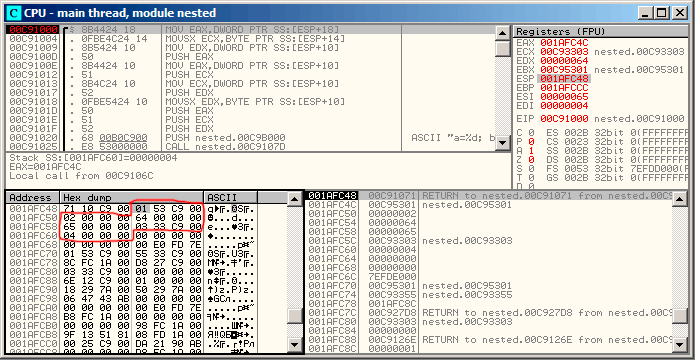
\includegraphics[scale=\FigScale]{patterns/15_structs/5_nested/olly.png}
\caption{\olly: Перед исполнением \printf}
\label{fig:nested_olly}
\end{figure}

Вот как расположены значения в памяти:
\begin{itemize}
\item \IT{(outer\_struct.a)} (байт) 1 + 3 байта случайного мусора;
\item \IT{(outer\_struct.b)} (32-битное слово) 2;
\item \IT{(inner\_struct.a)} (32-битное слово) 0x64 (100);
\item \IT{(inner\_struct.b)} (32-битное слово) 0x65 (101);
\item \IT{(outer\_struct.d)} (байт) 3 + 3 байта случайного мусора;
\item \IT{(outer\_struct.e)} (32-битное слово) 4.
\end{itemize}

}
\section{\RU{Работа с битовыми полями в структуре}\EN{Bit fields in a structure}}

\input{patterns/15_structs/6_bitfields/cpuid/main}
\input{patterns/15_structs/6_bitfields/float/main}

\subsection{\Exercises}

\begin{itemize}
	\item \url{http://challenges.re/71}
	\item \url{http://challenges.re/72}
\end{itemize}





\ifx\LITE\undefined
\chapter{\RU{Объединения (union)}\EN{Unions}}

\section{\IFRU{Пример генератора случайных чисел}{Pseudo-random number generator example}}

\IFRU{Если нам нужны случайные значения с плавающей запятой в интервале от 0 до 1, самое простое это взять
\ac{PRNG} вроде Mersenne twister выдающий случайные 32-битные числа в виде DWORD, преобразовать
это число в \Tfloat и затем разделить на \TT{RAND\_MAX} (\TT{0xFFFFFFFF} в данном случае) ~--- 
полученное число будет в интервале от 0 до 1.}
{If we need float random numbers from 0 to 1, the most simplest thing is to use \ac{PRNG} like
Mersenne twister produces random 32-bit values in DWORD form, transform this value to \Tfloat and then
dividing it by \TT{RAND\_MAX} (\TT{0xFFFFFFFF} in our case)~---value we got will be in 0..1 interval.}

\IFRU{Но как известно, операция деления ~--- это медленная операция. 
Сможем ли мы избежать её, как в случае с делением через умножение?}
{But as we know, division operation is slow.
Will it be possible to get rid of it, as in case of division by multiplication?}
~(\ref{sec:divisionbynine})

\index{IEEE 754}
\IFRU{Вспомним состав числа с плавающей запятой: это бит знака, биты мантиссы и биты экспоненты. 
Для получения случайного числа, нам нужно просто заполнить случайными битами все биты мантиссы!}
{Let's recall what float number consisted of: sign bit, significand bits and exponent bits.
We need just to store random bits to all significand bits for getting random float number!}

\IFRU{Экспонента не может быть нулевой (иначе число будет денормализованным), 
так что в эти биты мы запишем \TT{01111111} ~--- 
это будет означать что экспонента равна единице. Далее заполняем мантиссу случайными битами, 
знак оставляем в виде 0 (что значит наше число положительное), и вуаля. 
Генерируемые числа будут в интервале от 1 до 2, так что нам еще нужно будет отнять единицу.}
{Exponent cannot be zero (number will be denormalized in this case), so we will store \TT{01111111} 
to exponent~---this means exponent will be 1. Then fill significand with random bits, set sign bit to
0 (which means positive number) and voilà.
Generated numbers will be in 1 to 2 interval, so we also must subtract 1 from it.}

\newcommand{\URLXOR}{\url{http://xor0110.wordpress.com/2010/09/24/how-to-generate-floating-point-random-numbers-efficiently}}

\IFRU{В моем примере\footnote{идея взята здесь: \URLXOR} 
применяется очень простой линейный конгруэнтный генератор случайных чисел, выдающий 32-битные числа.
Генератор инициализируется текущим временем в стиле UNIX.}
{Very simple linear congruential random numbers generator is used in my 
example\footnote{idea was taken from: \URLXOR}, produces 32-bit numbers. 
The PRNG initializing by current time in UNIX-style.}

\IFRU{Далее, тип \Tfloat представляется в виде \IT{union} ~--- это конструкция \CCpp позволяющая 
интерпретировать часть памти по-разному. В нашем случае, мы можем создать переменную типа \TT{union} 
и затем обращаться к ней как к \Tfloat или как к \IT{uint32\_t}. Можно сказать, что это хак, причем грязный.}
{Then, \Tfloat type represented as \IT{union}~---it is the \CCpp construction enabling us
to interpret piece of memory as differently typed.
In our case, we are able to create a variable
of \TT{union} type and then access to it as it is \Tfloat or as it is \IT{uint32\_t}. 
It can be said, it is just a hack. A dirty one.}

\lstinputlisting{patterns/17_unions/FPU_PRNG.cpp}

\lstinputlisting[caption=MSVC 2010 (\Ox)]{patterns/17_unions/FPU_PRNG_msvc_2010_Ox_\LANG.asm}

\IFRU{А результат GCC будет почти таким же.}{GCC produces very similar code.}



\newcommand{\comp}{\TT{comp()}\xspace}
\chapter{\RU{Указатели на функции}\EN{Pointers to functions}}
\label{sec:pointerstofunctions}

\index{\CLanguageElements!\Pointers}
\RU{Указатель на функцию, в целом, как и любой другой указатель, просто адрес указывающий на начало функции 
в сегменте кода.}
\EN{Pointer to function, as any other pointer, is just an address of function beginning in its code segment.}

\index{Callbacks}
\RU{Это применяется часто в т.н. callback-ах}\EN{It is often used in callbacks}
\footnote{\url{http://en.wikipedia.org/wiki/Callback_(computer_science)}}.

\RU{Известные примеры:}\EN{Well-known examples are:}

\begin{itemize}
\item
\qsort\footnote{\url{http://en.wikipedia.org/wiki/Qsort_(C_standard_library)}},
{\TT{atexit()}}\footnote{\url{http://www.opengroup.org/onlinepubs/009695399/functions/atexit.html}} \RU{из стандартной библиотеки Си}\EN{from the standard C library}; 
\item
\RU{сигналы в *NIX ОС}\EN{signals in *NIX OS}\footnote{\url{http://en.wikipedia.org/wiki/Signal.h}};
\item
\RU{запуск тредов}\EN{thread starting}: \TT{CreateThread()} (win32), \TT{pthread\_create()} (POSIX);
\item
\RU{множество функций win32, например}\EN{a lot of win32 functions, e.g.} \TT{EnumChildWindows()}\footnote{\url{http://msdn.microsoft.com/en-us/library/ms633494(VS.85).aspx}}.
\end{itemize}

\index{\CStandardLibrary!qsort()}
\RU{Итак, функция \qsort это реализация алгоритма ``быстрой сортировки''. 
Функция может сортировать что угодно, 
любые типы данных, но при условии, что вы имеете функцию сравнения двух элементов данных и 
\qsort может вызывать её.}
\EN{So, \qsort function is a \CCpp standard library quicksort implementation. The functions is able to sort
anything, any types of data, if you have a function for two elements comparison and \qsort is able
to call it.}

\RU{Эта функция сравнения может определяться так:}\EN{The comparison function can be defined as:}

\begin{lstlisting}
int (*compare)(const void *, const void *)
\end{lstlisting}

\RU{Воспользуемся немного модифицированным примером, который я нашел вот}
\EN{Let's use slightly modified example I found} \href{http://cplus.about.com/od/learningc/ss/pointers2_8.htm}
{\RU{здесь}\EN{here}}:

\lstinputlisting[numbers=left,label=qsort_c_src]{patterns/18_pointers_to_functions/17_1.c}

\section{MSVC}

\RU{Компилируем в MSVC 2010 (я убрал некоторые части для краткости) с опцией \Ox}
\EN{Let's compile it in MSVC 2010 (I omitted some parts for the sake of brevity) with \Ox option}:

\lstinputlisting[caption=\Optimizing MSVC 2010: /Ox /GS- /MD]{patterns/18_pointers_to_functions/17_2_msvc_Ox.asm}

\RU{Ничего особо удивительного здесь мы не видим. В качестве четвертого аргумента, 
в \qsort просто передается адрес метки \TT{\_comp}, где собственно и располагается функция \comp.}
\EN{Nothing surprising so far.
As a fourth argument, an address of label \TT{\_comp} is passed, that is just a place
where function \comp located.}

\RU{Как \qsort вызывает её?}\EN{How \qsort calling it?}

\index{Windows!MSVCR80.DLL}
\RU{Посмотрим в MSVCR80.DLL (эта DLL куда в MSVC вынесены функции из стандартных библиотек Си):}
\EN{Let's take a look into this function located in MSVCR80.DLL (a MSVC DLL module with C standard library functions):}

\lstinputlisting[caption=MSVCR80.DLL]{patterns/18_pointers_to_functions/17_3_MSVCR.lst}

\TT{comp}\EMDASH{}\RU{это четвертый аргумент функции. 
Здесь просто передается управление по адресу указанному в \TT{comp}. 
Перед этим подготавливается два аргумента для функции \comp. 
Далее, проверяется результат её выполнения.}
\EN{is fourth function argument.
Here the control is just passed to the address in the \TT{comp} argument.
Before it, two arguments prepared for \comp. Its result is checked after its execution.}

\RU{Вот почему использование указателей на функции ~--- это опасно. 
Во-первых, если вызвать \qsort с неправильным указателем на функцию, 
то \qsort, дойдя до этого вызова, может передать управление неизвестно куда, 
процесс упадет, и эту ошибку можно будет найти не сразу.}
\EN{That's why it is dangerous to use pointers to functions.
First of all, if you call \qsort with incorrect pointer to function, \qsort may pass control
to incorrect point, a process may crash and this bug will be hard to find.}

\RU{Во-вторых, типизация callback-функции должна строго соблюдаться, 
вызов не той функции с не теми аргументами не того типа, 
может привести к плачевным результатам, 
хотя падение процесса это и не проблема, проблема ~--- это найти ошибку, ведь компилятор 
на стадии компиляции может вас и не предупредить о потенциальных неприятностях.}
\EN{Second reason is the callback function types must comply strictly, calling wrong function
with wrong arguments of wrong types may lead to serious problems, however, process crashing is not a 
big problem~---big problem is to determine a reason of crashing~---because compiler may be 
silent about potential trouble while compiling.}

\subsection{MSVC + \olly}
\index{\olly}

\RU{Загрузим наш пример в \olly и установим брякпойнт на ф-ции \comp}
\EN{Let's load our example into \olly and set breakpoint on \comp function}.

\RU{Как значения сравниваются, мы можем увидеть во время самого первого вызова \comp}
\EN{How values are compared we can see at the very first \comp call}: \figname \ref{fig:qsort_olly1}.
\RU{Для удобства, }\olly \RU{показывает сравниваемые значения в окне под окном кода}
\EN{shows compared values in the window under code window, for convenience}.
\RU{Мы можем так же увидеть что}\EN{We can also see that the} \ac{SP} \RU{указывает на}\EN{pointing to} 
\ac{RA} \RU{где находится место в ф-ции}\EN{where the place in} 
\qsort \EN{function is }(\RU{на самом деле, находится в}\EN{actually located in} \TT{MSVCR100.DLL}).

\RU{Трассируя}\EN{By tracing} (F8) \RU{до инструкции}\EN{until} \TT{RETN} 
\RU{и нажав F8 еще один раз, мы возвращаемся в ф-цию}\EN{instruction, and pressing F8 one more time, 
we returning into} \qsort\EN{ function}: \figname \ref{fig:qsort_olly2}.
\RU{Это был вызов ф-ции сравнения}\EN{That was a call to comparison function}.

\RU{Вот также скриншот момента второго вызова ф-ции}\EN{Here is also screenshot of the moment of the 
second call of} \comp\EMDASH{}\RU{теперь сравниваемые значения другие}
\EN{now values to be compared are different}:
\figname \ref{fig:qsort_olly3}.

\begin{figure}[H]
\centering
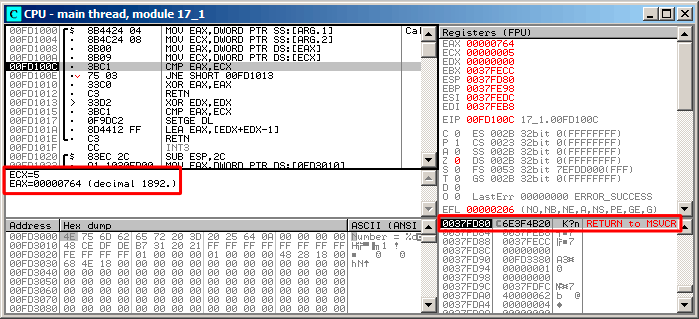
\includegraphics[scale=\FigScale]{patterns/18_pointers_to_functions/olly1.png}
\caption{\olly: \RU{первый вызов}\EN{first call of} \comp}
\label{fig:qsort_olly1}
\end{figure}

\begin{figure}[H]
\centering
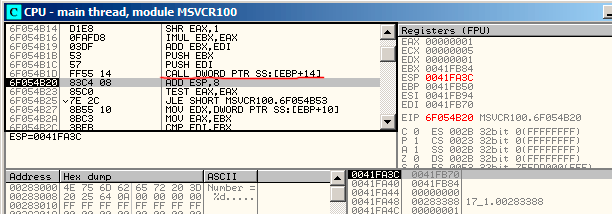
\includegraphics[scale=\FigScale]{patterns/18_pointers_to_functions/olly2.png}
\caption{\olly: \RU{код в}\EN{the code in} \qsort \RU{сразу после вызова}\EN{right after} \comp\EN{ call}}
\label{fig:qsort_olly2}
\end{figure}

\begin{figure}[H]
\centering
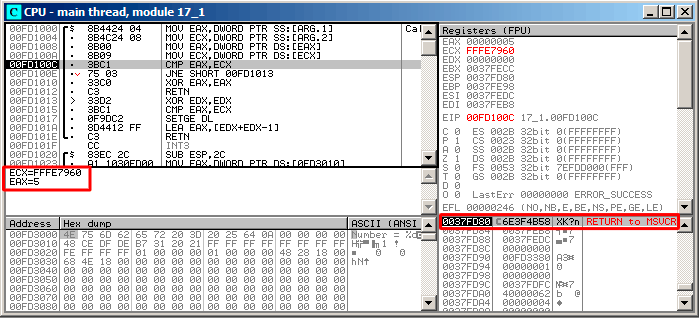
\includegraphics[scale=\FigScale]{patterns/18_pointers_to_functions/olly3.png}
\caption{\olly: \RU{второй вызов}\EN{second call of} \comp}
\label{fig:qsort_olly3}
\end{figure}

\subsection{MSVC + tracer}
\index{tracer}

\RU{Посмотрим, какие пары сравниваются}\EN{Let's also see, which pairs are compared}.
\RU{Эти 10 чисел будут сортироваться}\EN{These 10 numbers are being sorted}: 
1892, 45, 200, -98, 4087, 5, -12345, 1087, 88, -100000.

\RU{Я нашел адрес первой инструкции}\EN{I found the address of the first} \CMP 
\RU{в}\EN{instruction in} \comp, \RU{и это}\EN{it is} \TT{0x0040100C} 
\RU{и я ставлю брякпойнт на нем}\EN{and I'm setting breakpoint on it}:

\begin{lstlisting}
tracer.exe -l:17_1.exe bpx=17_1.exe!0x0040100C
\end{lstlisting}

\RU{Получаю информацию о регистрах на брякпойнте}
\EN{I'm getting information about registers at breakpoint}:

\begin{lstlisting}
PID=4336|New process 17_1.exe
(0) 17_1.exe!0x40100c
EAX=0x00000764 EBX=0x0051f7c8 ECX=0x00000005 EDX=0x00000000
ESI=0x0051f7d8 EDI=0x0051f7b4 EBP=0x0051f794 ESP=0x0051f67c
EIP=0x0028100c
FLAGS=IF
(0) 17_1.exe!0x40100c
EAX=0x00000005 EBX=0x0051f7c8 ECX=0xfffe7960 EDX=0x00000000
ESI=0x0051f7d8 EDI=0x0051f7b4 EBP=0x0051f794 ESP=0x0051f67c
EIP=0x0028100c
FLAGS=PF ZF IF
(0) 17_1.exe!0x40100c
EAX=0x00000764 EBX=0x0051f7c8 ECX=0x00000005 EDX=0x00000000
ESI=0x0051f7d8 EDI=0x0051f7b4 EBP=0x0051f794 ESP=0x0051f67c
EIP=0x0028100c
FLAGS=CF PF ZF IF
...
\end{lstlisting}

\RU{Я отфильтровал}\EN{I filtered out} \TT{EAX} \AndENRU \TT{ECX} \RU{и получил}\EN{and got}:

\begin{lstlisting}
EAX=0x00000764 ECX=0x00000005
EAX=0x00000005 ECX=0xfffe7960
EAX=0x00000764 ECX=0x00000005
EAX=0x0000002d ECX=0x00000005
EAX=0x00000058 ECX=0x00000005
EAX=0x0000043f ECX=0x00000005
EAX=0xffffcfc7 ECX=0x00000005
EAX=0x000000c8 ECX=0x00000005
EAX=0xffffff9e ECX=0x00000005
EAX=0x00000ff7 ECX=0x00000005
EAX=0x00000ff7 ECX=0x00000005
EAX=0xffffff9e ECX=0x00000005
EAX=0xffffff9e ECX=0x00000005
EAX=0xffffcfc7 ECX=0xfffe7960
EAX=0x00000005 ECX=0xffffcfc7
EAX=0xffffff9e ECX=0x00000005
EAX=0xffffcfc7 ECX=0xfffe7960
EAX=0xffffff9e ECX=0xffffcfc7
EAX=0xffffcfc7 ECX=0xfffe7960
EAX=0x000000c8 ECX=0x00000ff7
EAX=0x0000002d ECX=0x00000ff7
EAX=0x0000043f ECX=0x00000ff7
EAX=0x00000058 ECX=0x00000ff7
EAX=0x00000764 ECX=0x00000ff7
EAX=0x000000c8 ECX=0x00000764
EAX=0x0000002d ECX=0x00000764
EAX=0x0000043f ECX=0x00000764
EAX=0x00000058 ECX=0x00000764
EAX=0x000000c8 ECX=0x00000058
EAX=0x0000002d ECX=0x000000c8
EAX=0x0000043f ECX=0x000000c8
EAX=0x000000c8 ECX=0x00000058
EAX=0x0000002d ECX=0x000000c8
EAX=0x0000002d ECX=0x00000058
\end{lstlisting}

\RU{Это}\EN{That's} 34 \RU{пары}\EN{pairs}.
\RU{Следовательно, алгоритму быстрой сортировки нужно 34 операции сравнения для сортировки этих
10-и чисел}\EN{Therefore, quick sort algorithm needs 34 comparison operations for sorting these 10 numbers}.

\subsection{MSVC + tracer (code coverage)}
\index{tracer}

\RU{Но можно также и воспользоваться возможностью tracer накапливать все возможные состояния регистров
и показать их в \IDA}\EN{We can also use tracer's feature to collect all possible register's values
and show them in \IDA}.

\RU{Трассируем все инструкции в ф-ции \comp}\EN{Let's trace all instructions in \comp function}:

\begin{lstlisting}
tracer.exe -l:17_1.exe bpf=17_1.exe!0x00401000,trace:cc
\end{lstlisting}

\RU{Получем .idc-скрипт для загрузки в \IDA и загружаем его}
\EN{We getting .idc-script for loading into \IDA and load it}: \figname \ref{fig:qsort_tracer_cc}.

\RU{Имя этой ф-ции (PtFuncCompare) дала \IDA}\EN{\IDA gave the function name (PtFuncCompare)}
\EMDASH{}\RU{видимо, потому что видит что указатель на эту ф-цию передается в \qsort}\EN{it seems,
because \IDA sees that pointer to this function is passed into \qsort}.

\RU{Мы видим что указатели $a$ и $b$ указывают на разные места внутри массива, 
но шаг между указателями --- 4, что логично, ведь в массиве хранятся 32-битные значения}
\EN{We see that $a$ and $b$ pointers are points to various places in array, but step between
points is 4---indeed, 32-bit values are stored in the array}.

\RU{Видно что инструкции по адресам}\EN{We see that the instructions at} \TT{0x401010} \AndENRU 
\TT{0x401012} \RU{никогда не исполнялись}\EN{was never executed} 
(\RU{они и остались белыми}\EN{so they leaved as white}): 
\RU{действительно, ф-ция}\EN{indeed,} \comp \RU{никогда не возвращала 0,
потому что в массиве нет одинаковых элементов}\EN{was never returned 0, because there no equal elements}.

\begin{figure}[H]
\centering
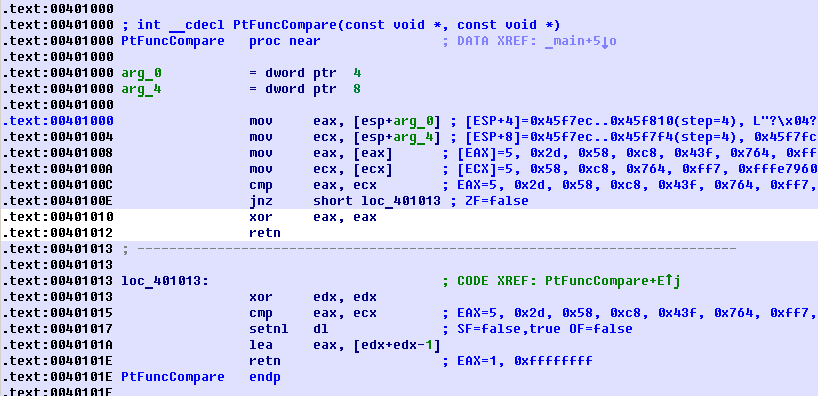
\includegraphics[scale=\FigScale]{patterns/18_pointers_to_functions/tracer_cc.png}
\caption{tracer \AndENRU IDA. N.B.: 
\RU{некоторые значения обрезаны справа}\EN{some values are cutted at right}}
\label{fig:qsort_tracer_cc}
\end{figure}

\section{GCC}

\RU{Не слишком большая разница}\EN{Not a big difference}:

\begin{lstlisting}[caption=GCC]
                lea     eax, [esp+40h+var_28]
                mov     [esp+40h+var_40], eax
                mov     [esp+40h+var_28], 764h
                mov     [esp+40h+var_24], 2Dh
                mov     [esp+40h+var_20], 0C8h
                mov     [esp+40h+var_1C], 0FFFFFF9Eh
                mov     [esp+40h+var_18], 0FF7h
                mov     [esp+40h+var_14], 5
                mov     [esp+40h+var_10], 0FFFFCFC7h
                mov     [esp+40h+var_C], 43Fh
                mov     [esp+40h+var_8], 58h
                mov     [esp+40h+var_4], 0FFFE7960h
                mov     [esp+40h+var_34], offset comp
                mov     [esp+40h+var_38], 4
                mov     [esp+40h+var_3C], 0Ah
                call    _qsort
\end{lstlisting}

\RU{Функция \comp}\EN{\comp function}:

\begin{lstlisting}
                public comp
comp            proc near

arg_0           = dword ptr  8
arg_4           = dword ptr  0Ch

                push    ebp
                mov     ebp, esp
                mov     eax, [ebp+arg_4]
                mov     ecx, [ebp+arg_0]
                mov     edx, [eax]
                xor     eax, eax
                cmp     [ecx], edx
                jnz     short loc_8048458
                pop     ebp
                retn
loc_8048458:
                setnl   al
                movzx   eax, al
                lea     eax, [eax+eax-1]
                pop     ebp
                retn
comp            endp
\end{lstlisting}

\index{Linux!libc.so.6}
\RU{Реализация \qsort находится в \TT{libc.so.6}, и представляет собой просто wrapper
\footnote{понятие близкое к \gls{thunk function}} для \TT{qsort\_r()}.}
\EN{\qsort implementation is located in the \TT{libc.so.6} and it is in fact just a wrapper
\footnote{a concept like \gls{thunk function}} for \TT{qsort\_r()}.}

\RU{Она, в свою очередь, вызывает \TT{quicksort()}, где есть вызовы определенной нами функции через 
переданный указатель:}
\EN{It will call then \TT{quicksort()}, where our defined function will be called via passed pointer:}


\begin{lstlisting}[caption=
(\RU{файл libc.so.6, версия glibc}\EN{file libc.so.6, glibc version}\EMDASH{}2.10.1)]

.text:0002DDF6                 mov     edx, [ebp+arg_10]
.text:0002DDF9                 mov     [esp+4], esi
.text:0002DDFD                 mov     [esp], edi
.text:0002DE00                 mov     [esp+8], edx
.text:0002DE04                 call    [ebp+arg_C]
...
\end{lstlisting}

\subsection{GCC + GDB (\RU{с исходными кодами}\EN{with source code})}
\index{GDB}

\RU{Очевидно, у нас есть исходный код нашего примера на Си (\ref{qsort_c_src}), 
так что мы можем установить брякпойнт (\TT{b}) на
номере строки}\EN{Obviously, we have a C-source code of our example (\ref{qsort_c_src}), 
so we can set breakpoint (\TT{b}) on line number}
(\RU{11-й --- это номер строки где происходит первое сравнение}\EN{11th---the line where 
first comparison is occurred}).
\RU{Нам также нужно скомпилировать наш пример с ключом \TT{-g}, чтобы в исполняемом файле была
полная отладочная информация}\EN{We also need to compile example with debugging information 
included (\TT{-g}), so the table
with addresses and corresponding line numbers is present}.
\RU{Мы можем так же выводить значения используя имена переменных}
\EN{We can also print values by variable name} (\TT{p}):
\RU{отладочная информация также содержит информацию о том, в каком регистре и/или элементе локального
стека находится какая переменная}\EN{debugging information also has information about which register and/or 
local stack element contain which variable}.

\index{Glibc}
\RU{Мы можем также увидеть стек}\EN{We can also see stack} (\TT{bt}) 
\RU{и обнаружить что в Glibc используется какая-то вспомогательная ф-ция с именем}
\EN{and find out that there are some intermediate function} 
\TT{msort\_with\_tmp()}\EN{ used in Glibc}.

\lstinputlisting[caption=GDB\RU{-сессия}\EN{ session}]{patterns/18_pointers_to_functions/GDB_source.txt}

\subsection{GCC + GDB (\RU{без исходных кодов}\EN{no source code})}
\index{GDB}

\RU{Но часто никаких исходных кодов нет вообще, так что мы можем дизассемблировать ф-цию \comp}
\EN{But often there are no source code at all, so we can disassemble \comp function} (\TT{disas}), 
\RU{найти самую первую инструкцию \CMP и установить брякпойнт}\EN{find the very first
\CMP instruction and set breakpoint} (\TT{b}) \RU{по этому адресу}\EN{at that address}.
\RU{На каждом брякпойнте мы будем видеть содержимое регистров}
\EN{At each breakpoint, we will dump all register contents} (\TT{info registers}).
\RU{Информация из стека так же доступна}\EN{Stack information is also available} (\TT{bt}), 
\RU{но частичная: здесь нет номеров строк для ф-ции \comp}
\EN{but partial: there are no line number information for \comp function}.

\lstinputlisting[caption=GDB\RU{-сессия}\EN{ session}]{patterns/18_pointers_to_functions/GDB_no_source.txt}


\fi
\ifdefined\ENGLISH
\section{64-bit values in 32-bit environment}
\label{sec:64bit_in_32_env}

In a 32-bit environment, \ac{GPR}'s are 32-bit, so 64-bit values are stored and passed as 32-bit value pairs
\footnote{By the way, 32-bit values are passed as pairs in 16-bit environment in the same way: \myref{win16_32bit_values}}.
\fi

\ifdefined\RUSSIAN
\section{64-битные значения в 32-битной среде}
\label{sec:64bit_in_32_env}

В среде, где \ac{GPR}-ы 32-битные, 64-битные значения хранятся и передаются как пары 32-битных значений
\footnote{Кстати, в 16-битной среде, 32-битные значения передаются 16-битными парами точно так же: \myref{win16_32bit_values}}.
\fi

\section{\RU{Возврат 64-битного значения}\EN{Returning of 64-bit value}}

\lstinputlisting{patterns/185_64bit_in_32_env/ret/0.c}

\subsection{x86}

\RU{64-битные значения в 32-битной среде возвращаются из ф-ций в паре регистров \EDX{}:\EAX{}.}
\EN{In a 32-bit environment, 64-bit values are returned from functions in the \EDX{}:\EAX{} register pair.}

\lstinputlisting[caption=\Optimizing MSVC 2010]{patterns/185_64bit_in_32_env/ret/0_MSVC_2010_Ox.asm}

\ifdefined\IncludeARM
\subsection{ARM}

\RU{64-битное значение возвращается в паре регистров R0-R1 ---
(R1 это старшая часть и R0 --- младшая часть):}
\EN{A 64-bit value is returned in the R0-R1 register pair 
(R1 is for the high part and R0 for the low part):}

\lstinputlisting[caption=\OptimizingKeilVI (\ARMMode)]{patterns/185_64bit_in_32_env/ret/Keil_ARM_O3.s}

\fi

\ifdefined\IncludeMIPS
\subsection{MIPS}

\RU{64-битное значение возвращается в паре регистров V0-V1 (\$2-\$3) ---
(V0 (\$2) это старшая часть и V1 (\$3) --- младшая часть):}
\EN{A 64-bit value is returned in the V0-V1 (\$2-\$3) register pair 
(V0 (\$2) is for the high part and V1 (\$3) for the low part):}

\lstinputlisting[caption=\Optimizing GCC 4.4.5 (assembly listing)]{patterns/185_64bit_in_32_env/ret/0_MIPS.s}

\lstinputlisting[caption=\Optimizing GCC 4.4.5 (IDA)]{patterns/185_64bit_in_32_env/ret/0_MIPS_IDA.lst}
\fi

\section{\RU{Передача аргументов, сложение, вычитание}\EN{Arguments passing, addition, subtraction}}

\lstinputlisting{patterns/185_64bit_in_32_env/passing_add_sub/1.c}

\subsection{x86}

\lstinputlisting[caption=\Optimizing MSVC 2012 /Ob1]{patterns/185_64bit_in_32_env/passing_add_sub/1_MSVC.asm}

\RU{В}\EN{We can see in the} \GTT{f\_add\_test()} \RU{видно, как каждое 64-битное число передается двумя 32-битными значениями,
сначала старшая часть, затем младшая}\EN{function that each 64-bit value is passed using two 32-bit values,
high part first, then low part}. \\
\\
\RU{Сложение и вычитание происходит также парами}\EN{Addition and subtraction occur in pairs as well}. \\
\\
\myindex{x86!\Instructions!ADC}
\RU{При сложении, в начале складываются младшие 32 бита}\EN{In addition, the low 32-bit part are added first}.
\RU{Если при сложении был перенос, выставляется флаг CF}\EN{If carry was occurred while adding, the CF flag is set}.
\RU{Следующая инструкция \INS{ADC} складывает старшие части чисел, но также прибавляет единицу если $CF=1$}
\EN{The following \INS{ADC} instruction adds the high parts of the values, and also adds 1 if $CF=1$}. \\
\\
\myindex{x86!\Instructions!SBB}
\RU{Вычитание также происходит парами}\EN{Subtraction also occurs in pairs}.
\RU{Первый}\EN{The first} \SUB \RU{может также включить флаг переноса CF, который затем будет проверяться в \INS{SBB}}
\EN{may also turn on the CF flag, which is to be checked in the subsequent \INS{SBB} instruction}:
\RU{если флаг переноса включен, то от результата отнимется единица}
\EN{if the carry flag is on, then 1 is also to be subtracted from the result}. \\
\\
\RU{Легко увидеть, как результат работы \GTT{f\_add()} затем передается в \printf{}}\EN{It is easy to see how
the \GTT{f\_add()} function result is then passed to \printf{}}.

\ifdefined\IncludeGCC
\lstinputlisting[caption=GCC 4.8.1 -O1 -fno-inline]{patterns/185_64bit_in_32_env/passing_add_sub/1_GCC.asm}

\RU{Код GCC почти такой же}\EN{GCC code is the same}.
\fi

\ifdefined\IncludeARM
\subsection{ARM}

\lstinputlisting[caption=\OptimizingKeilVI (\ARMMode)]{patterns/185_64bit_in_32_env/passing_add_sub/Keil_ARM_O3.s}

\myindex{ARM!\Instructions!ADDS}
\myindex{ARM!\Instructions!SUBS}
\myindex{ARM!\Instructions!ADC}
\myindex{ARM!\Instructions!SBC}
\RU{Первое 64-битное значение передается в паре регистров R0 и R1, второе --- в паре R2 и R3.}
\EN{The first 64-bit value is passed in R0 and R1 register pair, the second in R2 and R3 register pair.}
\RU{В ARM также есть инструкция ADC (учитывающая флаг переноса) и SBC (\q{subtract with carry} --- вычесть
с переносом).}
\EN{ARM has the ADC instruction as well (which counts carry flag) and SBC (\q{subtract with carry}).}

\RU{Важная вещь: когда младшие части слагаются/вычитаются, используются инструкции ADDS и SUBS с суффиксом
-S.}
\EN{Important thing: when the low parts are added/subtracted, ADDS and SUBS instructions with -S suffix are used.}
\RU{Суффикс -S означает \q{set flags} (установить флаги), а флаги (особенно флаг переноса) это то что однозначно
нужно последующим инструкциями ADC/SBC.}
\EN{The -S suffix stands for \q{set flags}, and flags (esp. carry flag) is what consequent ADC/SBC instructions
definitely need.}

\RU{А иначе инструкции без суффикса -S здесь вполне бы подошли (ADD и SUB).}
\EN{Otherwise, instructions without the -S suffix would do the job (ADD and SUB).}

\fi

\ifdefined\IncludeMIPS
\subsection{MIPS}

\lstinputlisting[caption=\Optimizing GCC 4.4.5 (IDA)]{patterns/185_64bit_in_32_env/passing_add_sub/MIPS_O3_IDA.lst.\LANG}

\RU{В MIPS нет регистра флагов, так что эта информация не присутствует после исполнения арифметических операций.}
\EN{MIPS has no flags register, so there is no such information present after the execution of arithmetic operations.}
\EN{So there are no instructions like x86's ADC and SBB.}
\RU{Так что здесь нет инструкций как ADC или SBB в x86.}
\RU{Чтобы получить информацию о том, был бы выставлен флаг переноса, происходит сравнение (используя инструкцию
\q{SLTU}), которая выставляет целевой регистр в 1 или 0.}
\EN{To know if the carry flag would be set, a comparison (using \q{SLTU} instruction) also occurs, 
which sets the destination register to 1 or 0.}
\RU{Эта 1 или 0 затем прибавляется к итоговому результату, или вычитается.}
\EN{This 1 or 0 is then added or subtracted to/from the final result.}

\fi

\section{\RU{Умножение, деление}\EN{Multiplication, division}}

\lstinputlisting{patterns/185_64bit_in_32_env/multdiv/2.c}

\subsection{x86}

\lstinputlisting[caption=\Optimizing MSVC 2012 /Ob1]{patterns/185_64bit_in_32_env/multdiv/2_MSVC.asm.\LANG}

\RU{Умножение и деление --- это более сложная операция, так что обычно, компилятор встраивает вызовы библиотечных функций,
делающих это}\EN{Multiplication and division are more complex operations, so usually the compiler embeds calls to
a library functions doing that}.

\ifx\LITE\undefined
\RU{Значение этих библиотечных функций, здесь}\EN{These functions are described here}: \myref{sec:MSVC_library_func}.
\fi

\ifdefined\IncludeGCC
\lstinputlisting[caption=\Optimizing GCC 4.8.1 -fno-inline]{patterns/185_64bit_in_32_env/multdiv/2_GCC.asm.\LANG}

\RU{GCC делает почти то же самое, тем не менее,
встраивает код умножения прямо в функцию, посчитав что так будет эффективнее}\EN{GCC does the expected, but the multiplication
code is inlined right in the function, thinking it could be more efficient}.
\RU{У GCC другие имена библиотечных функций}\EN{GCC has different library function names}: \myref{sec:GCC_library_func}.
\fi

\ifdefined\IncludeARM
\subsection{ARM}

\RU{Keil для режима Thumb вставляет вызовы библиотечных функций:}
\EN{Keil for Thumb mode inserts library subroutine calls:}

\lstinputlisting[caption=\OptimizingKeilVI (\ThumbMode)]{patterns/185_64bit_in_32_env/multdiv/Keil_thumb_O3.s}

\RU{Keil для режима ARM, тем не менее, может сгенерировать код для умножения 64-битных чисел:}
\EN{Keil for ARM mode, on the other hand, is able to produce 64-bit multiplication code:}

\lstinputlisting[caption=\OptimizingKeilVI (\ARMMode)]{patterns/185_64bit_in_32_env/multdiv/Keil_ARM_O3.s}
% TODO add explanation
\fi

\ifdefined\IncludeMIPS
\subsection{MIPS}

\Optimizing GCC \ForENRU MIPS 
\EN{can generate 64-bit multiplication code, but has to call a library routine for 64-bit division:}
\RU{может генерировать код для 64-битного умножения, но для 64-битного деления приходится вызывать библиотечную функцию:}

\lstinputlisting[caption=\Optimizing GCC 4.4.5 (IDA)]{patterns/185_64bit_in_32_env/multdiv/MIPS_O3_IDA.lst}

\RU{Тут также много \ac{NOP}-ов, это возможно заполнение delay slot-ов после инструкции умножения (она ведь работает
медленнее прочих инструкций), но я не однозначно уверен.}
\EN{There are a lot of \ac{NOP}s, probably delay slots filled after the multiplication instruction (it's slower
than other instructions, after all), but I'm not completely sure.}

% TODO add explanation
\fi

\section{\RU{Сдвиг вправо}\EN{Shifting right}}

\lstinputlisting{patterns/185_64bit_in_32_env/shifting/3.c}

\subsection{x86}

\lstinputlisting[caption=\Optimizing MSVC 2012 /Ob1]{patterns/185_64bit_in_32_env/shifting/3_MSVC.asm}

\ifdefined\IncludeGCC
\lstinputlisting[caption=\Optimizing GCC 4.8.1 -fno-inline]{patterns/185_64bit_in_32_env/shifting/3_GCC.asm}
\fi

\index{x86!\Instructions!SHRD}
\RU{Сдвиг происходит также в две операции: в начале сдвигается младшая часть, затем старшая}
\EN{Shifting also occurs in two passes: first the lower part is shifted, then the higher part}.
\RU{Но младшая часть сдвигается
при помощи инструкции \INS{SHRD}, она сдвигает значение в \EDX{} на 7 бит, но подтягивает новые биты из \EAX{}, т.е. из старшей части.}
\EN{But the lower part is shifted with the help of the \INS{SHRD} instruction, it shifts the value of \EDX{} by 7 bits, but pulls new bits
from \EAX{}, i.e., from the higher part.}
\RU{Старшая часть сдвигается более известной инструкцией \SHR{}: действительно, ведь освободившиеся биты в старшей части нужно
просто заполнить нулями}\EN{The higher part is shifted using the more popular \SHR{} instruction: indeed, the freed bits in the higher part
must be filled with zeroes}.

\ifdefined\IncludeARM
\subsection{ARM}

\RU{В ARM нет такой инструкции как SHRD в x86, так что компилятору Keil приходится всё это делать,
используя простые сдвиги и операции \q{ИЛИ}:}
\EN{ARM doesn't have such instruction as SHRD in x86, so the Keil compiler ought to do this using simple shifts
and OR operations:}

\lstinputlisting[caption=\OptimizingKeilVI (\ARMMode)]{patterns/185_64bit_in_32_env/shifting/Keil_ARM_O3.s}

\lstinputlisting[caption=\OptimizingKeilVI (\ThumbMode)]{patterns/185_64bit_in_32_env/shifting/Keil_thumb_O3.s}
% TODO add explanation
\fi

\ifdefined\IncludeMIPS
\subsection{MIPS}

\ifdefined\IncludeGCC
\EN{GCC for MIPS follows the same algorithm as Keil does for Thumb mode:}
\RU{GCC для MIPS реализует тот же алгоритм, что сделал Keil для режима Thumb:}

\lstinputlisting[caption=\Optimizing GCC 4.4.5 (IDA)]{patterns/185_64bit_in_32_env/shifting/MIPS_O3_IDA.lst}
\fi

% TODO add explanation
\fi

\section{\RU{Конвертирование 32-битного значения в 64-битное}\EN{Converting 32-bit value into 64-bit one}}
\label{subsec:sign_extending_32_to_64}

\lstinputlisting{patterns/185_64bit_in_32_env/conversion/4.c}

\subsection{x86}

\lstinputlisting[caption=\Optimizing MSVC 2012]{patterns/185_64bit_in_32_env/conversion/MSVC2012_Ox.asm}

\RU{Здесь появляется необходимость расширить 32-битное знаковое значение в 64-битное знаковое.}
\EN{Here we also run into necessity to extend a 32-bit signed value into a 64-bit signed one.}
\RU{Конвертировать беззнаковые значения очень просто: нужно просто выставить в 0 все биты в старшей части}
\EN{Unsigned values are converted straightforwardly: all bits in the higher part must be set to 0}.
\RU{Но для знаковых типов это не подходит: знак числа должен быть скопирован в старшую часть числа-результата}
\EN{But this is not appropriate for signed data types: the sign has to be copied into the higher part of the resulting number}.
\myindex{x86!\Instructions!CDQ}
\RU{Здесь это делает инструкция \INS{CDQ}, она берет входное значение в \EAX{}, расширяет его до 64-битного,
и оставляет его в паре регистров \EDX{}:\EAX{}}
\EN{The \INS{CDQ} instruction does that here, it takes its input value in \EAX{}, extends it to 64-bit and leaves it
in the \EDX{}:\EAX{} register pair}.
\RU{Иными словами, инструкция \INS{CDQ} узнает знак числа в \EAX{} (просто берет самый старший бит в \EAX{}) и в зависимости от этого,
выставляет все 32 бита в \EDX{} в 0 или в 1}\EN{In other words, \INS{CDQ} gets the number sign from \EAX{} (by getting the
most significant bit in \EAX{}), and depending of it, sets all 32 bits in \EDX{} to 0 or 1}.
\RU{Её работа в каком-то смысле напоминает работу инструкции \MOVSX{}}\EN{Its operation is somewhat
similar to the \MOVSX{} instruction}.

\ifdefined\IncludeARM
\subsection{ARM}

\lstinputlisting[caption=\OptimizingKeilVI (\ARMMode)]{patterns/185_64bit_in_32_env/conversion/Keil_ARM_O3.s}

\RU{Keil для ARM работает иначе: он просто сдвигает (арифметически) входное значение на 31 бит вправо.}
\EN{Keil for ARM is different: it just arithmetically shifts right the input value by 31 bits.}
\RU{Как мы знаем, бит знака это \ac{MSB}, и арифметический сдвиг копирует бит знака в \q{появляющихся} битах.}
\EN{As we know, the sign bit is \ac{MSB}, and the arithmetical shift copies the sign bit into the \q{emerged} bits.}
\RU{Так что после инструкции \q{ASR r1,r0,\#31}, R1 будет содержать 0xFFFFFFFF если входное значение
было отрицательным, или 0 в противном случае.}
\EN{So after \q{ASR r1,r0,\#31}, R1 containing 0xFFFFFFFF if the input value was negative
and 0 otherwise.}
\RU{R1 содержит старшую часть возвращаемого 64-битного значения.}
\EN{R1 contains the high part of the resulting 64-bit value.}

\RU{Другими словами, этот код просто копирует \ac{MSB} (бит знака) из входного значения в R0 во все
биты старшей 32-битной части итогового 64-битного значения.}
\EN{In other words, this code just copies the \ac{MSB} (sign bit) from the input value in R0 to all bits
of the high 32-bit part of the resulting 64-bit value.}

\fi

\ifdefined\IncludeMIPS
\subsection{MIPS}

\ifdefined\IncludeGCC
\EN{GCC for MIPS does the same as Keil did for ARM mode:}
\RU{GCC для MIPS делает то же, что сделал Keil для режима ARM:}

\lstinputlisting[caption=\Optimizing GCC 4.4.5 (IDA)]{patterns/185_64bit_in_32_env/conversion/MIPS_O3_IDA.lst}
\fi

\fi



\ifx\LITE\undefined
\chapter{SIMD}

\label{SIMD_x86}
\ac{SIMD} \RU{это акроним}\EN{is an acronym}: \IT{Single Instruction, Multiple Data}.

\RU{Как можно судить по названию, это обработка множества данных исполняя только одну инструкцию.}
\EN{As it is said, it is multiple data processing using only one instruction.}

\RU{Как и \ac{FPU}, эта подсистема процессора выглядит так же отдельным процессором внутри x86.}
\EN{As \ac{FPU}, that \ac{CPU} subsystem looks like separate processor inside x86.}

\index{x86!MMX}
\RU{SIMD в x86 начался с MMX. Появилось 8 64-битных регистров MM0-MM7.}
\EN{SIMD began as MMX in x86. 8 new 64-bit registers appeared: MM0-MM7.}

\RU{Каждый MMX-регистр может содержать 2 32-битных значения, 4 16-битных или же 8 байт. 
Например, складывая значения двух MMX-регистров, можно складывать одновременно 8 8-битных значений.}
\EN{Each MMX register may hold 2 32-bit values, 4 16-bit values or 8 bytes.
For example, it is possible to add 8 8-bit values (bytes) simultaneously by adding two values in MMX-registers.}

\RU{Простой пример, это некий графический редактор, который хранит открытое изображение как двумерный массив. 
Когда пользователь меняет яркость изображения, редактору нужно, например, прибавить некий коэффициент 
ко всем пикселям, или отнять. 
Для простоты можно представить, что изображение у нас бело-серо-черное и каждый пиксель занимает один байт, 
то с помощью MMX можно менять яркость сразу у восьми пикселей.}
\EN{One simple example is graphics editor, representing image as a two dimensional array.
When user change image brightness, the editor must add a coefficient to each pixel value, or to subtract.
For the sake of brevity, our image may be grayscale and each pixel defined by one 8-bit byte, then it is possible
to change brightness of 8 pixels simultaneously.}
\RU{Кстати, вот причина почему в SIMD присутствуют инструкции с \IT{насыщением} (\IT{saturation}).}
\EN{By the way, it's also a reason why \IT{saturation} instructions present in SIMD.}
\RU{Когда пользователь в графическом редакторе изменяет яркость, переполнение и антипереполнение (\IT{underflow})
не нужны, так что в SIMD имеются, например, инструкции сложения, которые ничего не будут прибавлять
если максимальное значение уже достигнуто, итд.}
\EN{When user changing brightness in graphics editor, overflow and underflow is not desirable, 
so there are addition instructions in SIMD which will not add anything if maximal value is reached, etc.}

\RU{Когда MMX только появилось, эти регистры на самом деле располагались в FPU-регистрах. 
Можно было использовать 
либо FPU либо MMX в одно и то же время. Можно подумать, что Intel решило немного сэкономить на транзисторах, 
но на самом деле причина такого симбиоза проще ~--- более старая \ac{OS} не знающая о дополнительных 
регистрах процессора не будет сохранять их во время переключения задач, а вот регистры FPU сохранять будет. 
Таким образом, процессор с MMX + старая \ac{OS} + задача использующая возможности MMX = все 
это может работать вместе.}
\EN{When MMX appeared, these registers was actually located in FPU registers. 
It was possible to use either FPU or MMX at the same time. One might think, Intel saved on transistors,
but in fact, the reason of such symbiosis is simpler~---older \ac{OS} may not aware 
of additional CPU registers would not save them at the context switching, but will save FPU registers.
Thus, MMX-enabled CPU + old \ac{OS} + process utilizing MMX features = that all will work together.}

\index{x86!SSE}
\index{x86!SSE2}
SSE\EMDASH\RU{это расширение регистров до 128 бит, теперь уже отдельно от FPU.}\EN{is extension of SIMD registers up to 128 bits, now separately from FPU.}

\index{x86!AVX}
AVX\EMDASH\RU{расширение регистров до 256 бит.}\EN{another extension to 256 bits.}

\RU{Немного о практическом применении.}\EN{Now about practical usage.}

\RU{Конечно же, копирование блоков в памяти (\TT{memcpy}), сравнение (\TT{memcmp}), и подобное.}
\EN{Of course, memory copy routines (\TT{memcpy}), memory comparing (\TT{memcmp}) and so on.}

\index{DES}
\RU{Еще пример: имеется алгоритм шифрования DES, который берет 64-битный блок, 56-битный ключ, 
шифрует блок с ключом и образуется 64-битный результат.
Алгоритм DES можно легко представить в виде очень большой электронной цифровой схемы, 
с проводами, элементами И, ИЛИ, НЕ.}
\EN{One more example: we got DES encryption algorithm, it takes 64-bit block, 56-bit key, encrypt block and produce 64-bit result.
DES algorithm may be considered as a very large electronic circuit, with wires and AND/OR/NOT gates.}

\label{bitslicedes}
\newcommand{\URLBS}{\url{http://go.yurichev.com/17329}}

\RU{Идея bitslice DES\footnote{\URLBS} ~--- это обработка сразу группы блоков и ключей одновременно. 
Скажем, на x86 переменная типа \IT{unsigned int} вмещает в себе 32 бита, так что там можно хранить 
промежуточные результаты сразу для 32-х блоков-ключей, используя 64+56 переменных типа \IT{unsigned int}.}
\EN{Bitslice DES\footnote{\URLBS}~---is an idea of processing group of blocks and keys simultaneously.
Let's say, variable of type \IT{unsigned int} on x86 may hold up to 32 bits, so, it is possible to store there
intermediate results for 32 blocks-keys pairs simultaneously, using 64+56 variables of \IT{unsigned int} type.}

\index{\oracle}
\RU{Я написал утилиту для перебора паролей/хешей \oracle (которые основаны на алгоритме DES), 
переделав алгоритм bitslice DES для SSE2 и AVX ~--- и теперь возможно шифровать одновременно 
128 или 256 блоков-ключей:}
\EN{I wrote an utility to brute-force \oracle passwords/hashes (ones based on DES),
slightly modified bitslice DES algorithm for SSE2 and AVX~---now it is possible to encrypt 128 
or 256 block-keys pairs simultaneously.}

\url{http://go.yurichev.com/17313}

% sections
\section{\RU{Векторизация}\EN{Vectorization}}

\newcommand{\URLVEC}{\href{http://en.wikipedia.org/wiki/Vectorization_(computer_science)}{Wikipedia: vectorization}}

\RU{Векторизация\footnote{\URLVEC} это когда у вас есть цикл, который берет на вход несколько массивов и выдает, 
например, один массив данных. 
Тело цикла берет некоторые элементы из входных массивов, что-то делает с ними и помещает в выходной. 
Важно, что операция применяемая ко всем элементам одна и та же. 
Векторизация ~--- это обрабатывать несколько элементов одновременно.}
\EN{Vectorization\footnote{\URLVEC}, for example, is when you have a loop taking couple of arrays at input and produces one array.
Loop body takes values from input arrays, do something and put result into output array.
It is important that there is only one single operation applied to each element.
Vectorization~---is to process several elements simultaneously.}

\RU{Векторизация ~--- это не самая новая технология: автор сих строк видел её по крайней мере на 
линейке суперкомпьютеров Cray Y-MP от 1988, когда работал на его версии-``лайт'' Cray Y-MP EL
\footnote{Удаленно. Он находится в музее суперкомпьютеров: \url{http://www.cray-cyber.org}}}
\EN{Vectorization is not very fresh technology: author of this textbook saw it at least on Cray Y-MP 
supercomputer line from 1988 when played with its ``lite'' version Cray Y-MP EL
\footnote{Remotely. It is installed in the museum of supercomputers: \url{http://www.cray-cyber.org}}}.

\RU{Например:}\EN{For example:}

\begin{lstlisting}
for (i = 0; i < 1024; i++)
{
    C[i] = A[i]*B[i];
}
\end{lstlisting}

\RU{Этот фрагмент кода берет элементы из A и B, перемножает и сохраняет результат в C.}
\EN{This fragment of code takes elements from A and B, multiplies them and save result into C.}

\index{x86!\Instructions!PLMULLD}
\index{x86!\Instructions!PLMULHW}
\newcommand{\PMULLD}{\IT{PMULLD} (\IT{\RU{Перемножить запакованные знаковые DWORD и сохранить младшую часть результата}
\EN{Multiply Packed Signed Dword Integers and Store Low Result}})}
\newcommand{\PMULHW}{\TT{PMULHW} (\IT{\RU{Перемножить запакованные знаковые DWORD и сохранить старшую часть результата}
\EN{Multiply Packed Signed Integers and Store High Result}})}

\RU{Если представить, что каждый элемент массива ~--- это 32-битный \Tint, то их можно загружать сразу 
по 4 из А в 128-битный XMM-регистр, 
из B в другой XMM-регистр и выполнив инструкцию \PMULLD{} и \PMULHW{}, можно получить 4 64-битных 
\glslink{product}{произведения} сразу.}
\EN{If each array element we have is 32-bit \Tint, then it is possible to load 4 elements from A into 128-bit 
XMM-register, from B to another XMM-registers, and by executing \PMULLD{} and \PMULHW{}, 
it is possible to get 4 64-bit \glspl{product} at once.}

\RU{Таким образом, тело цикла исполняется $1024/4$ раза вместо 1024, что в 4 раза меньше, и, конечно, быстрее.}
\EN{Thus, loop body count is $1024/4$ instead of $1024$, that is 4 times less and, of course, faster.}

\newcommand{\URLINTELVEC}{\href{http://www.intel.com/intelpress/sum_vmmx.htm}{Excerpt: Effective Automatic Vectorization}}

\subsection{\RU{Пример сложения}\EN{Addition example}}

\index{Intel C++}
\RU{Некоторые компиляторы умеют делать автоматическую векторизацию в простых случаях, 
например Intel C++\footnote{Еще о том, как Intel C++ умеет автоматически векторизовать циклы: \URLINTELVEC}.}
\EN{Some compilers can do vectorization automatically in a simple cases, 
e.g., Intel C++\footnote{More about Intel C++ automatic vectorization: \URLINTELVEC}.}

\RU{Я написал очень простую функцию:}\EN{I wrote tiny function:}

\begin{lstlisting}
int f (int sz, int *ar1, int *ar2, int *ar3)
{
	for (int i=0; i<sz; i++)
		ar3[i]=ar1[i]+ar2[i];

	return 0;
};
\end{lstlisting}

\subsubsection{Intel C++}

\RU{Компилирую при помощи}\EN{Let's compile it with} Intel C++ 11.1.051 win32:

\begin{verbatim}
icl intel.cpp /QaxSSE2 /Faintel.asm /Ox
\end{verbatim}

\RU{Имеем такое (в \IDA):}\EN{We got (in \IDA):}

\lstinputlisting{patterns/19_SIMD/18_1_en.asm}

\RU{Инструкции, имеющие отношение к SSE2 это:}\EN{SSE2-related instructions are:}
\index{x86!\Instructions!MOVDQA}
\index{x86!\Instructions!MOVDQU}
\index{x86!\Instructions!PADDD}
\begin{itemize}
\item
\MOVDQU (\IT{Move Unaligned Double Quadword})\EMDASH\RU{она просто загружает 16 байт из памяти в XMM-регистр}
\EN{it just load 16 bytes from memory into a XMM-register}.

\item
\PADDD (\IT{Add Packed Integers})\EMDASH\RU{складывает сразу 4 пары 32-битных чисел и оставляет в первом операнде результат. 
Кстати, если произойдет переполнение, то исключения не произойдет и никакие флаги не установятся, 
запишутся просто младшие 32 бита результата. 
Если один из операндов \PADDD ~--- адрес значения в памяти, 
то требуется чтобы адрес был выровнен по 16-байтной границе. Если он не выровнен, произойдет исключение
\footnote{О выравнивании данных см. также: \URLWPDA}.}
\EN{adding 4 pairs of 32-bit numbers and leaving result in first operand.
By the way, no exception raised in case of overflow and no flags will be set, just low 32-bit of result will
be stored.
If one of \PADDD operands is address of value in memory,
then address must be aligned on a 16-byte boundary. If it is not aligned, exception will be occurred
\footnote{More about data aligning: \URLWPDA}.}

\item
\MOVDQA (\IT{Move Aligned Double Quadword})\EMDASH\RU{тоже что и \MOVDQU, только подразумевает 
что адрес в памяти выровнен по 16-байтной границе. 
Если он не выровнен, произойдет исключение. 
\MOVDQA работает быстрее чем \MOVDQU, но требует вышеозначенного.}
\EN{the same as \MOVDQU, but requires address of value in memory to be aligned on a 16-bit border.
If it is not aligned, exception will be raised.
\MOVDQA works faster than \MOVDQU, but requires aforesaid.}

\end{itemize}

\RU{Итак, эти SSE2-инструкции исполнятся только в том случае если еще осталось просуммировать 
4 пары переменных типа \Tint плюс если указатель \TT{ar3} выровнен по 16-байтной границе.}
\EN{So, these SSE2-instructions will be executed only in case if there are more 4 pairs to work on
plus pointer \TT{ar3} is aligned on a 16-byte boundary.}

\RU{Более того, если еще и \TT{ar2} выровнен по 16-байтной границе, то будет выполняться этот фрагмент кода:}
\EN{More than that, if \TT{ar2} is aligned on a 16-byte boundary as well, this fragment of code will be executed:}

\begin{lstlisting}
movdqu  xmm0, xmmword ptr [ebx+edi*4] ; ar1+i*4
paddd   xmm0, xmmword ptr [esi+edi*4] ; ar2+i*4
movdqa  xmmword ptr [eax+edi*4], xmm0 ; ar3+i*4
\end{lstlisting}

\RU{А иначе, значение из \TT{ar2} загрузится в \XMM{0} используя инструкцию \MOVDQU, 
которая не требует выровненного указателя, зато может работать чуть медленнее:}
\EN{Otherwise, value from \TT{ar2} will be loaded into \XMM{0} using \MOVDQU,
it does not require aligned pointer, but may work slower:}

\begin{lstlisting}
movdqu  xmm1, xmmword ptr [ebx+edi*4] ; ar1+i*4
movdqu  xmm0, xmmword ptr [esi+edi*4] ; ar2+i*4 is not 16-byte aligned, so load it to xmm0
paddd   xmm1, xmm0
movdqa  xmmword ptr [eax+edi*4], xmm1 ; ar3+i*4
\end{lstlisting}

\RU{А во всех остальных случаях, будет исполняться код, который был бы, как если бы не была 
включена поддержка SSE2.}
\EN{In all other cases, non-SSE2 code will be executed.}

\subsubsection{GCC}

\newcommand{\URLGCCVEC}{\url{http://gcc.gnu.org/projects/tree-ssa/vectorization.html}}

\RU{Но и GCC умеет кое-что векторизировать\footnote{Подробнее о векторизации в GCC: \URLGCCVEC}, 
если компилировать с опциями \Othree и включить поддержку SSE2: \TT{-msse2}.}
\EN{GCC may also vectorize in a simple cases\footnote{More about GCC vectorization support: \URLGCCVEC},
if to use \Othree option and to turn on SSE2 support: \TT{-msse2}.}

\RU{Вот что вышло}\EN{What we got} (GCC 4.4.1):

\lstinputlisting{patterns/19_SIMD/18_2_gcc_O3.asm}

\RU{Почти то же самое, хотя и не так дотошно как Intel C++.}
\EN{Almost the same, however, not as meticulously as Intel C++ doing it.}

\ifx\RUSSIAN\undefined
\subsection{\RU{Пример копирования блоков}\EN{Memory copy example}}
\label{vec_memcpy}

Let's revisit simple memcpy() example (\ref{loop_memcpy}):

\lstinputlisting{memcpy.c}

And that's what optimizing GCC 4.9.1 did:

\lstinputlisting[caption=\Optimizing GCC 4.9.1 x64]{patterns/19_SIMD/memcpy_GCC49_x64_O3.s}
\fi

\section{\RU{Реализация \strlen при помощи SIMD}\EN{SIMD \strlen implementation}}

\newcommand{\URLMSDNSSE}{\href{http://go.yurichev.com/17262}{MSDN: MMX, SSE, and SSE2 Intrinsics}}

\RU{Прежде всего, следует заметить, что SIMD-инструкции можно вставлять в \CCpp код при помощи специальных 
макросов\footnote{\URLMSDNSSE}. В MSVC, часть находится в файле \TT{intrin.h}.}
\EN{It should be noted that the \ac{SIMD} instructions can be inserted in \CCpp code via 
special macros\footnote{\URLMSDNSSE}.
For MSVC, some of them are located in the \TT{intrin.h} file.}

\newcommand{\URLSTRLEN}{http://go.yurichev.com/17330}

\index{\CStandardLibrary!strlen()}
\RU{Имеется возможность реализовать функцию \strlen\footnote{strlen() ~--- стандартная функция Си 
для подсчета длины строки} при помощи SIMD-инструкций, работающий в 2-2.5 раза быстрее обычной реализации. 
Эта функция будет загружать в XMM-регистр сразу 16 байт и проверять каждый на ноль}
\EN{It is possible to implement the \strlen function\footnote{strlen()~---standard C library function for calculating
string length} using SIMD instructions that works 2-2.5 times faster than the common implementation.
This function will load 16 characters into a XMM-register and check each against zero}
\footnote{\RU{Пример базируется на исходнике отсюда: \url{\URLSTRLEN}.}
\EN{The example is based on source code from: \url{\URLSTRLEN}.}}.

\lstinputlisting{patterns/19_SIMD/18_3.c}

\RU{Компилируем в MSVC 2010 с опцией \Ox:}\EN{Let's compile it in MSVC 2010 with \Ox option:}

\lstinputlisting[caption=\Optimizing MSVC 2010]{patterns/19_SIMD/18_4_msvc_Ox.asm.\LANG}

\RU{Итак, прежде всего, мы проверяем указатель \TT{str}, выровнен ли он по 16-байтной границе. 
Если нет, то мы вызовем обычную реализацию \strlen.}
\EN{First, we check if the \TT{str} pointer is aligned on a 16-byte boundary.
If not, we call the generic \strlen implementation.}

\RU{Далее мы загружаем по 16 байт в регистр \XMM{1} при помощи команды \MOVDQA.}
\EN{Then, we load the next 16 bytes into the \XMM{1} register using \MOVDQA.}

\RU{Наблюдательный читатель может спросить, почему в этом месте мы не можем использовать \MOVDQU, 
которая может загружать откуда угодно не взирая на факт, выровнен ли указатель?}
\EN{An observant reader might ask, why can't \MOVDQU be used here since it can load data from the memory
regardless pointer alignment?}

\RU{Да, можно было бы сделать вот как: если указатель выровнен, загружаем используя \MOVDQA, 
иначе используем работающую чуть медленнее \MOVDQU.}
\EN{Yes, it might be done in this way: if the pointer is aligned, load data using \MOVDQA,
if not~---use the slower \MOVDQU.}

\RU{Однако здесь кроется не сразу заметная проблема, которая проявляется вот в чем:}
\EN{But here we are may hit another caveat:}

\index{Page (memory)}
\newcommand{\URLPAGE}{\href{http://go.yurichev.com/17136}{wikipedia}}

\RU{В \ac{OS} линии \gls{Windows NT} (и не только), память выделяется страницами по 4 KiB (4096 байт). 
Каждый win32-процесс якобы имеет в наличии 4 GiB, но на самом деле, 
только некоторые части этого адресного пространства присоединены к реальной физической памяти. 
Если процесс обратится к блоку памяти, которого не существует, сработает исключение. 
Так работает \ac{VM}\footnote{\URLPAGE}.}
\EN{In the \gls{Windows NT} line of \ac{OS} (but not limited to it), memory is allocated by pages of 4 KiB (4096 bytes).
Each win32-process has 4 GiB available, but in fact, only some parts
of the address space are connected to real physical memory.
If the process is accessing an absent memory block, an exception will be raised.
That's how \ac{VM} works\footnote{\URLPAGE}.}

\RU{Так вот, функция, читающая сразу по 16 байт, имеет возможность нечаянно вылезти за границу 
выделенного блока памяти. 
Предположим, \ac{OS} выделила программе 8192 (0x2000) байт по адресу 0x008c0000. 
Таким образом, блок занимает байты с адреса 0x008c0000 по 0x008c1fff включительно.}
\EN{So, a function loading 16 bytes at once  may step over the border of an allocated memory block.
Let's say that the \ac{OS} has allocated 8192 (0x2000) bytes at address 0x008c0000.
Thus, the block is the bytes starting from address 0x008c0000 to 0x008c1fff inclusive.}

\RU{За этим блоком, то есть начиная с адреса 0x008c2000 нет вообще ничего, т.е., \ac{OS} не выделяла там память. 
Обращение к памяти начиная с этого адреса вызовет исключение.}
\EN{After the block, that is, starting from address 0x008c2000 there is nothing at all, e.g. the \ac{OS} not allocated
any memory there.
Any attempt to access memory starting from that address will raise an exception.}

\RU{И предположим, что программа хранит некую строку из, скажем, пяти символов почти в самом конце блока, 
что не является преступлением:}
\EN{And let's consider the example in which the program is holding a string that contains 5 characters almost at the end of a block,
and that is not a crime.}

\begin{center}
  \begin{tabular}{ | l | l | }
    \hline
        0x008c1ff8 & 'h' \\
        0x008c1ff9 & 'e' \\
        0x008c1ffa & 'l' \\
        0x008c1ffb & 'l' \\
        0x008c1ffc & 'o' \\
        0x008c1ffd & '\textbackslash{}x00' \\
        0x008c1ffe & \RU{здесь случайный мусор}\EN{random noise} \\
        0x008c1fff & \RU{здесь случайный мусор}\EN{random noise} \\
    \hline
  \end{tabular}
\end{center}

\RU{В обычных условиях, программа вызывает \strlen передав ей указатель на строку \TT{'hello'} 
лежащую по адресу 0x008c1ff8. 
\strlen будет читать по одному байту до 0x008c1ffd, где ноль, и здесь она закончит работу.}
\EN{So, in normal conditions the program calls \strlen, passing it a pointer to the string \TT{'hello'} 
placed in memory at address 0x008c1ff8.
\strlen will read one byte at a time until 0x008c1ffd, where there's a zero byte, and it will stop working.}

\RU{Теперь, если мы напишем свою реализацию \strlen читающую сразу по 16 байт, с любого адреса, 
будь он выровнен по 16-байтной границе или нет, 
\MOVDQU попытается загрузить 16 байт с адреса 0x008c1ff8 по 0x008c2008, и произойдет исключение. 
Это ситуация которой, конечно, хочется избежать.}
\EN{Now if we implement our own \strlen reading 16 byte at once, starting at any address, aligned or not,
\MOVDQU may attempt to load 16 bytes at once at address 0x008c1ff8 up to 0x008c2008, 
and then an exception will be raised.
That situation is to be avoided, of course.}

\RU{Поэтому мы будем работать только с адресами, выровненными по 16 байт, что в сочетании со знанием 
что размер страницы \ac{OS} также, как правило, выровнен по 16 байт, 
даст некоторую гарантию что наша функция не будет пытаться читать из мест в невыделенной памяти.}
\EN{So then we'll work only with the addresses aligned on a 16 byte boundary, which in combination with the knowledge
that the \ac{OS}' page size is usually aligned on a 16-byte boundary gives us some warranty that our function will not
read from unallocated memory.}

\RU{Вернемся к нашей функции}\EN{Let's get back to our function}.

\index{x86!\Instructions!PXOR}
\verb|_mm_setzero_si128()|\EMDASH\RU{это макрос, генерирующий \TT{pxor xmm0, xmm0} ~--- инструкция просто обнуляет регистр \XMM{0}.}
\EN{is a macro generating \TT{pxor xmm0, xmm0}~---it just clears the \XMM{0} register}.

\verb|_mm_load_si128()|\EMDASH\RU{это макрос для \MOVDQA, он просто загружает 16 байт по адресу из указателя в \XMM{1}.}
\EN{is a macro for \MOVDQA, it just loads 16 bytes from the address into the \XMM{1} register.}

\index{x86!\Instructions!PCMPEQB}
\verb|_mm_cmpeq_epi8()|\EMDASH\RU{это макрос для \PCMPEQB, это инструкция, которая 
побайтово сравнивает значения из двух XMM регистров.} 
\EN{is a macro for \PCMPEQB, an instruction that compares two XMM-registers bytewise.}

\RU{И если какой-то из байт равен другому, то в результирующем значении будет выставлено на месте этого 
байта \TT{0xff}, либо 0, если байты не были равны.}
\EN{And if some byte was equals to the one in the other register, there will be \TT{0xff} at this point in the result or 0 if otherwise.}

\RU{Например.}\EN{For example.}

\begin{verbatim}
XMM1: 11223344556677880000000000000000
XMM0: 11ab3444007877881111111111111111
\end{verbatim}

\RU{После исполнения \TT{pcmpeqb xmm1, xmm0}, регистр \XMM{1} будет содержать:}
\EN{After the execution of \TT{pcmpeqb xmm1, xmm0}, the \XMM{1} register will contain:}

\begin{verbatim}
XMM1: ff0000ff0000ffff0000000000000000
\end{verbatim}

\RU{Эта инструкция в нашем случае, сравнивает каждый 16-байтный блок с блоком состоящим из 16-и нулевых байт, 
выставленным в \XMM{0} при помощи \TT{pxor xmm0, xmm0}.}
\EN{In our case, this instruction compares each 16-byte block with a block of 16 zero-bytes,
which was set in the \XMM{0} register by \TT{pxor xmm0, xmm0}.}

\index{x86!\Instructions!PMOVMSKB}
\RU{Следующий макрос \TT{\_mm\_movemask\_epi8()} ~--- это инструкция \TT{PMOVMSKB}.}
\EN{The next macro is \TT{\_mm\_movemask\_epi8()}~---that is the \TT{PMOVMSKB} instruction.}

\RU{Она очень удобна как раз для использования в паре с \PCMPEQB.}
\EN{It is very useful with \PCMPEQB.}

\TT{pmovmskb eax, xmm1}

\RU{Эта инструкция выставит самый первый бит \EAX в единицу, если старший бит первого байта в 
регистре \XMM{1} является единицей. 
Иными словами, если первый байт в регистре \XMM{1} является \TT{0xff}, то первый бит в \EAX будет также единицей, 
иначе нулем.}
\EN{This instruction will set first \EAX bit to 1 if the most significant bit of the first byte in \XMM{1} is $1$.
In other words, if the first byte of the \XMM{1} register is \TT{0xff}, the first bit of \EAX will be set to 1, too.}

\RU{Если второй байт в регистре \XMM{1} является \TT{0xff}, то второй бит в \EAX также будет единицей. 
Иными словами, инструкция отвечает на вопрос, ``какие из байт в \XMM{1} являются \TT{0xff}?''
В результате приготовит 16 бит и запишет в \EAX. Остальные биты в \EAX обнулятся.}
\EN{If the second byte in the \XMM{1} register is \TT{0xff}, then the second bit in \EAX will be set to 1.
In other words, the instruction is answering the question ``which bytes in \XMM{1} are \TT{0xff}?''
and will return 16 bits in the \EAX register. The other bits in the \EAX register will be cleared.}

\RU{Кстати, не забывайте также вот о какой особенности нашего алгоритма.}
\EN{By the way, do not forget about this quirk of our algorithm.}
\RU{На вход может прийти 16 байт вроде}\EN{There might be 16 bytes in the input like}:

\begin{center}
\begin{bytefield}[endianness=big,bitwidth=0.05\linewidth]{16}
\bitheader{15,14,13,12,11,10,9,3,2,1,0} \\
\bitbox{1}{``h''} & 
\bitbox{1}{``e''} & 
\bitbox{1}{``l''} & 
\bitbox{1}{``l''} & 
\bitbox{1}{``o''} & 
\bitbox{1}{0} & 
\bitbox{7}{\garbage{}} & 
\bitbox{1}{0} &
\bitbox{2}{\garbage{}} & 
\end{bytefield}
\end{center}

\RU{Это строка \TT{'hello'}, после нее терминирующий ноль, затем немного мусора в памяти.}
\EN{It is the \TT{'hello'} string, terminating zero, and some random noise in memory.}
\RU{Если мы загрузим эти 16 байт в \XMM{1} и сравним с нулевым \XMM{0}, то в итоге получим такое 
\footnote{Я использую здесь порядок с \ac{MSB} до \ac{LSB}}:}
\EN{If we load these 16 bytes into \XMM{1} and compare them with the zeroed \XMM{0}, we will get something like
\footnote{I use here order from \ac{MSB} to \ac{LSB}}:}

\begin{verbatim}
XMM1: 0000ff00000000000000ff0000000000
\end{verbatim}

\RU{Это означает что инструкция сравнения обнаружила два нулевых байта, что и не удивительно.}
\EN{This means that the instruction found two zero bytes, and it is not surprising.}

\RU{\TT{PMOVMSKB} в нашем случае подготовит \EAX вот так (в двоичном представлении):} 
\EN{\TT{PMOVMSKB} in our case will set \EAX to (in binary representation):} \IT{0010000000100000b}.

\RU{Совершенно очевидно, что далее наша функция должна учитывать только первый встретившийся
нулевой бит и игнорировать все остальное.}
\EN{Obviously, our function must take only the first zero bit and ignore the rest.}

\index{x86!\Instructions!BSF}
\label{instruction_BSF}
\RU{Следующая инструкция\EMDASH}\EN{The next instruction is }\TT{BSF} (\IT{Bit Scan Forward}). 
\RU{Это инструкция находит самый младший бит во втором операнде и записывает его позицию в первый операнд.}
\EN{This instruction finds the first bit set to 1 and stores its position into the first operand.}

\begin{verbatim}
EAX=0010000000100000b
\end{verbatim}

\RU{После исполнения этой инструкции \TT{bsf eax, eax}, в \EAX будет 5, что означает, 
что единица найдена в пятой позиции (считая с нуля).}
\EN{After the execution of \TT{bsf eax, eax}, \EAX will contain 5, meaning 
1 was found at the 5th bit position (starting from zero).}

\RU{Для использования этой инструкции, в MSVC также имеется макрос}
\EN{MSVC has a macro for this instruction:} \TT{\_BitScanForward}.

\RU{А дальше все просто. Если нулевой байт найден, его позиция прибавляется к тому что 
мы уже насчитали и возвращается результат.}
\EN{Now it is simple. If a zero byte was found, its position is added to what we have already counted and now we have 
the return result.}

\RU{Почти всё.}\EN{Almost all.}

\RU{Кстати, следует также отметить, что компилятор MSVC сгенерировал два тела цикла сразу, для оптимизации.}
\EN{By the way, it is also should be noted that the MSVC compiler emitted two loop bodies side by side, for optimization.}

\RU{Кстати, в SSE 4.2 (который появился в Intel Core i7) все эти манипуляции со строками могут быть еще проще:}
\EN{By the way, SSE 4.2 (that appeared in Intel Core i7) offers more instructions where these string manipulations might be
even easier:} \url{http://go.yurichev.com/17331}


\fi
\chapter{\RU{64 бита}\EN{64 bits}}

\section{x86-64}
\myindex{x86-64}
\label{x86-64}

\RU{Это расширение x86-архитуктуры до 64 бит.}\EN{It is a 64-bit extension to the x86 architecture.}

\RU{С точки зрения начинающего reverse engineer-а, наиболее важные отличия от 32-битного x86 это:}
\EN{From the reverse engineer's perspective, the most important changes are:}

\myindex{\CLanguageElements!\Pointers}
\begin{itemize}

\item
\RU{Почти все регистры (кроме FPU и SIMD) расширены до 64-бит и получили префикс R-. 
И еще 8 регистров добавлено. 
В итоге имеются эти \ac{GPR}-ы:}
\EN{Almost all registers (except FPU and SIMD) were extended to 64 bits and got a R- prefix.
8 additional registers wer added.
Now \ac{GPR}'s are:} \RAX, \RBX, \RCX, \RDX, 
\RBP, \RSP, \RSI, \RDI, \Reg{8}, \Reg{9}, \Reg{10}, 
\Reg{11}, \Reg{12}, \Reg{13}, \Reg{14}, \Reg{15}. 

\RU{К ним также можно обращаться так же, как и прежде. Например, для доступа к младшим 32 битам \RAX 
можно использовать \EAX:}
\EN{It is still possible to access the \IT{older} register parts as usual. 
For example, it is possible to access the lower 32-bit part of the \RAX register using \EAX:}

\RegTableOne{RAX}{EAX}{AX}{AH}{AL}

\RU{У новых регистров \GTT{R8-R15} также имеются их \IT{младшие части}: \GTT{R8D-R15D} 
(младшие 32-битные части), 
\GTT{R8W-R15W} (младшие 16-битные части), \GTT{R8L-R15L} (младшие 8-битные части).}
\EN{The new \GTT{R8-R15} registers also have their \IT{lower parts}: \GTT{R8D-R15D} (lower 32-bit parts),
\GTT{R8W-R15W} (lower 16-bit parts), \GTT{R8L-R15L} (lower 8-bit parts).}

\RegTableFour{R8}{R8D}{R8W}{R8L}

\RU{Удвоено количество SIMD-регистров: с 8 до 16:}
\EN{The number of SIMD registers was doubled from 8 to 16:} \XMM{0}-\XMM{15}.

\item
\RU{В win64 передача всех параметров немного иная, это немного похоже на fastcall 
(\myref{fastcall})
.
Первые 4 аргумента записываются в регистры \RCX, \RDX, \Reg{8}, \Reg{9}, а остальные ~--- в стек. 
Вызывающая функция также должна подготовить место из 32 байт чтобы вызываемая функция могла сохранить 
там первые 4 аргумента и использовать эти регистры по своему усмотрению. 
Короткие функции могут использовать аргументы прямо из регистров, но б\'{о}льшие функции могут сохранять 
их значения на будущее.}
\EN{In Win64, the function calling convention is slightly different, somewhat resembling fastcall
(\myref{fastcall})
.
The first 4 arguments are stored in the \RCX, \RDX, \Reg{8}, \Reg{9} registers, the rest~---in the stack.
The \gls{caller} function must also allocate 32 bytes so the \gls{callee} may save there 4 first arguments and use these 
registers for its own needs.
Short functions may use arguments just from registers, but larger ones may save their values on the stack.}

\RU{Соглашение }System V AMD64 ABI (Linux, *BSD, \MacOSX)\cite{SysVABI} \RU{также напоминает}\EN{also somewhat resembles}
fastcall, \RU{использует 6 регистров}\EN{it uses 6 registers} 
\RDI, \RSI, \RDX, \RCX, \Reg{8}, \Reg{9} \RU{для первых шести аргументов}\EN{for the first 6 arguments}.
\RU{Остальные передаются через стек}\EN{All the rest are passed via the stack}.

\RU{См. также в соответствующем разделе о способах передачи аргументов через стек}
\EN{See also the section on calling conventions}~(\myref{sec:callingconventions}).

\item
\RU{\Tint в \CCpp остается 32-битным для совместимости.}
\EN{The \CCpp \Tint type is still 32-bit for compatibility.}

\item
\RU{Все указатели теперь 64-битные}\EN{All pointers are 64-bit now}.

\RU{На это иногда сетуют: ведь теперь для хранения всех указателей нужно в 2 раза больше места 
в памяти, в т.ч. и в кэш-памяти, не смотря на то что x64-процессоры могут адресовать только 48 бит
внешней \ac{RAM}.}
\EN{This provokes irritation sometimes: now one needs twice as much memory for storing pointers,
including cache memory, despite the fact that x64 \ac{CPU}s can address only 48 bits of external 
\ac{RAM}.}

\end{itemize}

\myindex{Register allocation}
\RU{Из-за того, что регистров общего пользования теперь вдвое больше, у компиляторов теперь больше 
свободного места для маневра, называемого \glslink{register allocator}{register allocation}.
Для нас это означает, что в итоговом коде будет меньше локальных переменных.}
\EN{Since now the number of registers is doubled, the compilers have more space for maneuvering called 
\glslink{register allocator}{register allocation}.
For us this implies that the emitted code containing less number of local variables.}

\myindex{DES}
\RU{Для примера, функция вычисляющая первый S-бокс алгоритма шифрования DES, 
она обрабатывает сразу 32/64/128/256 значений, в зависимости от типа \GTT{DES\_type} (uint32, uint64, SSE2 или AVX), 
методом bitslice DES (больше об этом методе читайте здесь~(\myref{bitslicedes})):}
\EN{For example, the function that calculates the first S-box of the DES encryption algorithm processes
32/64/128/256 values at once (depending on \GTT{DES\_type} type (uint32, uint64, SSE2 or AVX)) 
using the bitslice DES method
(read more about this technique here ~(\myref{bitslicedes})):}

\lstinputlisting{patterns/20_x64/19_1.c}

\RU{Здесь много локальных переменных. Конечно, далеко не все они будут в локальном стеке. 
Компилируем обычным MSVC 2008 с опцией \Ox:}
\EN{There are a lot of local variables. 
Of course, not all those going into the local stack.
Let's compile it with MSVC 2008 with \Ox option:}

\lstinputlisting[caption=\Optimizing MSVC 2008]{patterns/20_x64/19_2_msvc_Ox.asm}

\RU{5 переменных компилятору пришлось разместить в локальном стеке.}
\EN{5 variables were allocated in the local stack by the compiler.}

\RU{Теперь попробуем то же самое только в 64-битной версии MSVC 2008:}
\EN{Now let's try the same thing in the 64-bit version of MSVC 2008:}

\lstinputlisting[caption=\Optimizing MSVC 2008]{patterns/20_x64/19_3_msvc_x64.asm}

\RU{Компилятор ничего не выделил в локальном стеке, а \GTT{x36} это синоним для \GTT{a5}.}
\EN{Nothing was allocated in the local stack by the compiler, \GTT{x36} is synonym for \GTT{a5}.}

\iffalse
% FIXME1 невнятно
\RU{Кстати, видно, что функция сохраняет регистры \RCX, \RDX в отведенных для 
этого вызываемой функцией местах, 
а \Reg{8} и \Reg{9} не сохраняет, а начинает использовать их сразу.}
\EN{By the way, we can see here that the function saved the \RCX and \RDX registers in space allocated by the \gls{caller},
but \Reg{8} and \Reg{9} were not saved but used from the beginning.}
\fi

\RU{Кстати, существуют процессоры с еще большим количеством \ac{GPR}, например, 
Itanium ~--- 128 регистров.}
\EN{By the way, there are CPUs with much more \ac{GPR}'s, e.g. Itanium (128 registers).}

\ifdefined\IncludeARM
\section{ARM}

\RU{64-битные инструкции появились в}\EN{64-bit instructions appeared in} ARMv8.
\fi

\section{\RU{Числа с плавающей запятой}\EN{Float point numbers}}

\RU{О том как происходит работа с числами с плавающей запятой в x86-64, читайте здесь: \myref{floating_SIMD}.}
\EN{How floating point numbers are processed in x86-64 is explained here: \myref{floating_SIMD}.}

\ifx\LITE\undefined
% FIXME divide this file into files...
\chapter{\RU{Работа с числами с плавающей запятой используя SIMD}\EN{Working with floating point numbers using SIMD}}

\label{floating_SIMD}
\index{IEEE 754}
\index{SIMD}
\index{SSE}
\index{SSE2}
\RU{Разумеется, FPU остался в x86-совместимых процессорах в то время, когда ввели расширения \ac{SIMD}}
\EN{Of course, the \ac{FPU} has remained in x86-compatible processors when the \ac{SIMD} extensions were added}.

\EN{The }\ac{SIMD}\RU{-расширения}\EN{ extensions} (SSE2) \RU{позволяют удобнее работать с числами с плавающей 
запятой}\EN{offer an easier way to work with floating-point numbers}.

\RU{Формат чисел остается тот же}\EN{The number format remains the same} (IEEE 754).

\index{x86-64}
\RU{Так что современные компиляторы (включая те, что компилируют под x86-64) 
обычно используют \ac{SIMD}-инструкции вместо FPU-инструкций.}\EN{So, modern compilers (including those generating
for x86-64) usually use \ac{SIMD} instructions instead of FPU ones.}

\RU{Это, можно сказать, хорошая новость, потому что работать с ними легче}
\EN{It can be said that it's good news, because it's easier to work with them}.

\RU{Примеры будем использовать из секции о FPU}\EN{We will reuse here the examples from the FPU section}: \myref{sec:FPU}.

\section{\RU{Простой пример}\EN{Simple example}}

\lstinputlisting{patterns/12_FPU/1_simple/simple.c}

\subsection{x64}

\lstinputlisting[caption=\Optimizing MSVC 2012 x64]{patterns/205_floating_SIMD/simple_MSVC_2012_x64_Ox.asm}

\RU{Собственно, входные значения с плавающей запятой передаются через регистры \XMM{0}-\XMM{3}, 
а остальные --- через стек}\EN{The input floating point values are passed in the \XMM{0}-\XMM{3} registers,
all the rest---via the stack}
\footnote{\href{http://go.yurichev.com/17263}{MSDN: Parameter Passing}}.

$a$ \RU{передается через}\EN{is passed in} \XMM{0}, $b$\EMDASH{}\RU{через}\EN{via} \XMM{1}.
\RU{Но XMM-регистры (как мы уже знаем из секции о \ac{SIMD}: \myref{SIMD_x86}) 128-битные, 
а значения типа \Tdouble --- 64-битные,
так что используется только младшая половина регистра}
\EN{The XMM-registers are 128-bit (as we know from the section about \ac{SIMD}: \myref{SIMD_x86}), 
but the \Tdouble values are 64 bit, so only lower register half is used}.

\index{x86!\Instructions!DIVSD}
\TT{DIVSD} \RU{это SSE-инструкция, означает}\EN{is an SSE-instruction that means} 
``Divide Scalar Double-Precision Floating-Point Values'', 
\RU{и просто делит значение типа \Tdouble на другое, лежащие в младших половинах операндов}\EN{it just divides
one value of type \Tdouble by another, stored in the lower halves of operands}.

\RU{Константы закодированы компилятором в формате IEEE 754}\EN{The constants are encoded by compiler in IEEE 754 format}.

\index{x86!\Instructions!MULSD}
\index{x86!\Instructions!ADDSD}
\TT{MULSD} \AndENRU \TT{ADDSD} \RU{работают так же, только производят умножение и сложение}
\EN{work just as the same, but do multiplication and addition}.

\RU{Результат работы ф-ции типа \Tdouble ф-ция оставляет в регистре \XMM{0}}
\EN{The result of the function's execution in type \Tdouble is left in the in \XMM{0} register}.\\
\\
\RU{Как работает неоптимизирующий MSVC}\EN{That is how non-optimizing MSVC works}:

\lstinputlisting[caption=MSVC 2012 x64]{patterns/205_floating_SIMD/simple_MSVC_2012_x64.asm}

\index{Shadow space}
\RU{Чуть более избыточно}\EN{Slightly redundant}. 
\RU{Входные аргументы сохраняются в}\EN{The input arguments are saved in the} ``shadow space'' (\myref{shadow_space}), 
\RU{причем, только младшие половины регистров, т.е., только 64-битные значения типа \Tdouble}
\EN{but only their lower register halves, i.e., only 64-bit values of type \Tdouble}.\\
\\
\RU{Результат работы компилятора GCC точно такой же}\EN{GCC produces the same code}.

\subsection{x86}

\RU{Я скомпилировал этот пример также и под x86. MSVC 2012 даже генерируя под x86, использует 
SSE2-инструкции:}\EN{I also compiled this example for x86. Despite the fact it's generating for x86, 
MSVC 2012 uses SSE2 instructions:}

\lstinputlisting[caption=\NonOptimizing MSVC 2012 x86]{patterns/205_floating_SIMD/simple_MSVC_2012_x86.asm}

\lstinputlisting[caption=\Optimizing MSVC 2012 x86]{patterns/205_floating_SIMD/simple_MSVC_2012_x86_Ox.asm}

\RU{Код почти такой же, правда есть пара отличий связанных с соглашениями о вызовах:}
\EN{It's almost the same code, however, there are some differences related to calling conventions:}
1) \RU{аргументы передаются не в XMM-регистрах, а через стек, как и прежде, в примерах с FPU (\myref{sec:FPU});}
\EN{the arguments are passed not in XMM registers, but in the stack, like in the FPU examples (\myref{sec:FPU});}
2) \RU{результат работы ф-ции возвращается через \ST{0} --- для этого он через стек
(через локальную переменную \TT{tv}) копируется из XMM-регистра в \ST{0}.}
\EN{the result of the function is returned in \ST{0} --- in order to do so, it's copied
(through local variable \TT{tv}) from one of the XMM registers to \ST{0}.}

\ifdefined\IncludeOlly
\clearpage
\RU{Попробуем соптимизированный пример в}\EN{Let's try the optimized example in} \olly:

\begin{figure}[H]
\centering
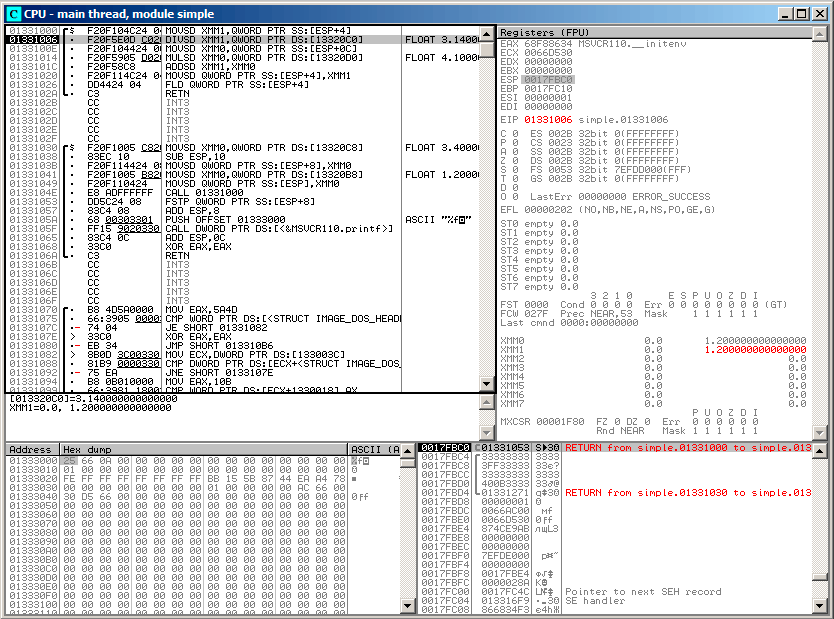
\includegraphics[scale=\FigScale]{patterns/205_floating_SIMD/simple_olly1.png}
\caption{\olly: \TT{MOVSD} \RU{загрузила значение}\EN{loads the value of} $a$ \RU{в}\EN{into} \XMM{1}}
\label{fig:FPU_SIMD_simple_olly1}
\end{figure}

\clearpage
\begin{figure}[H]
\centering
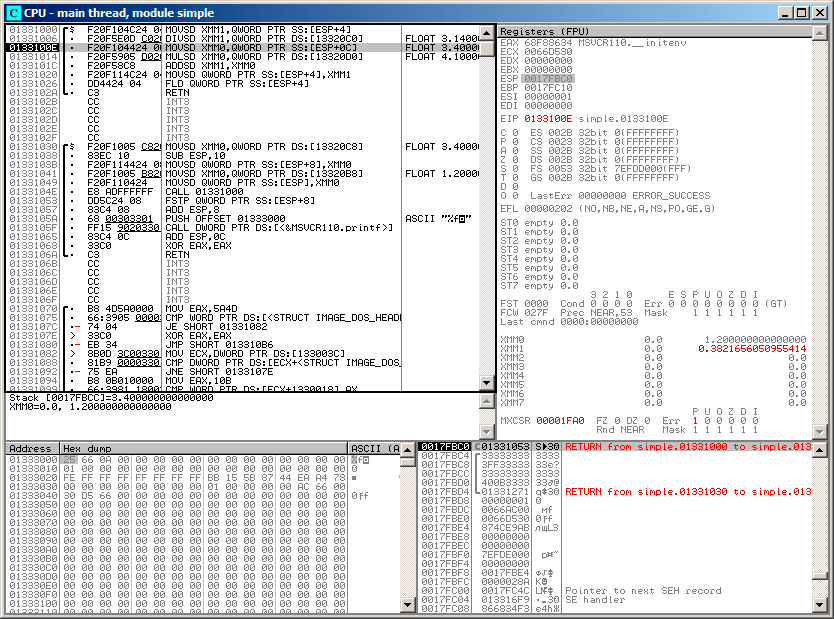
\includegraphics[scale=\FigScale]{patterns/205_floating_SIMD/simple_olly2.png}
\caption{\olly: \TT{DIVSD} \RU{вычислила}\EN{calculated} \gls{quotient} 
\RU{и оставила его в}\EN{and stored it in} \XMM{1}}
\label{fig:FPU_SIMD_simple_olly2}
\end{figure}

\clearpage
\begin{figure}[H]
\centering
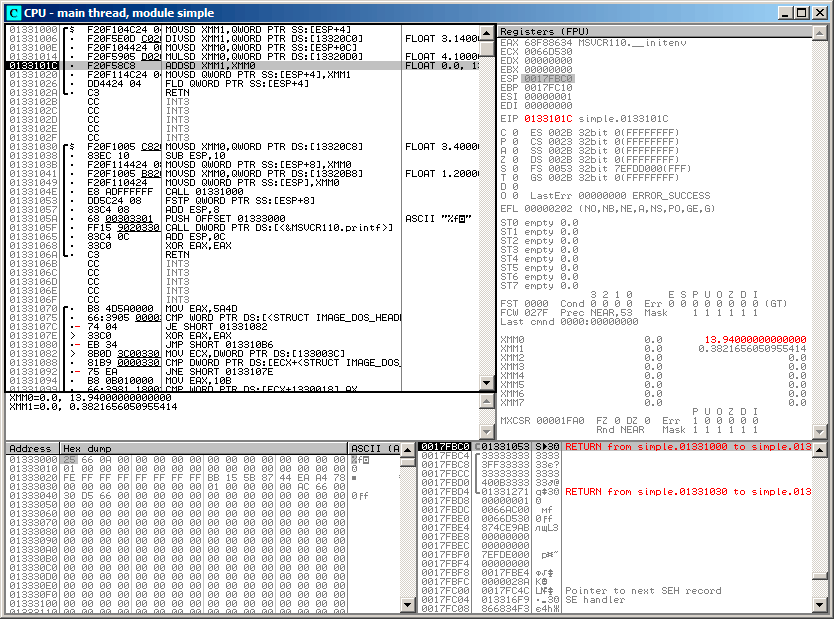
\includegraphics[scale=\FigScale]{patterns/205_floating_SIMD/simple_olly3.png}
\caption{\olly: \TT{MULSD} \RU{вычислила}\EN{calculated} \gls{product} \RU{и оставила его в}\EN{and stored it
in} \XMM{0}}
\label{fig:FPU_SIMD_simple_olly3}
\end{figure}

\clearpage
\begin{figure}[H]
\centering
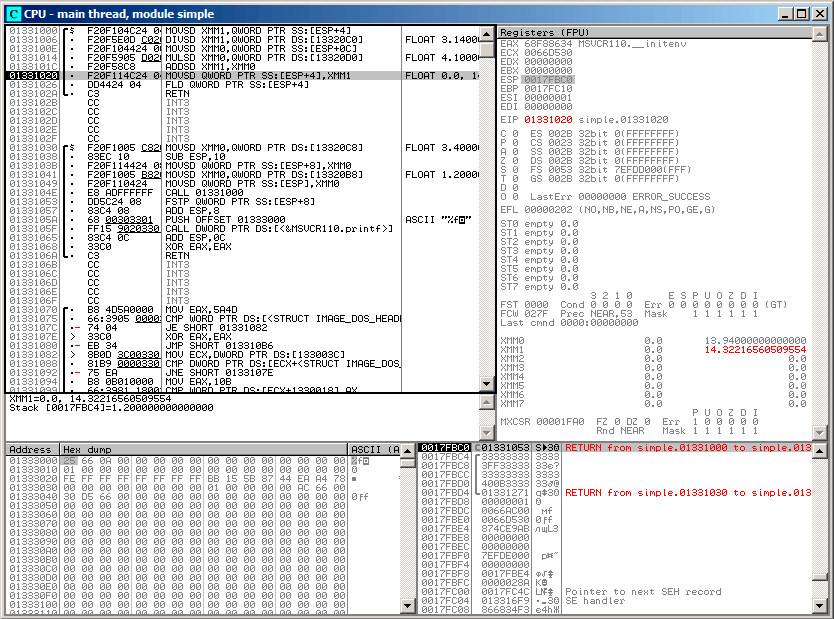
\includegraphics[scale=\FigScale]{patterns/205_floating_SIMD/simple_olly4.png}
\caption{\olly: \TT{ADDSD} \RU{прибавила значение в}\EN{adds value in} \XMM{0} \RU{к}\EN{to} \XMM{1}}
\label{fig:FPU_SIMD_simple_olly4}
\end{figure}

\clearpage
\begin{figure}[H]
\centering
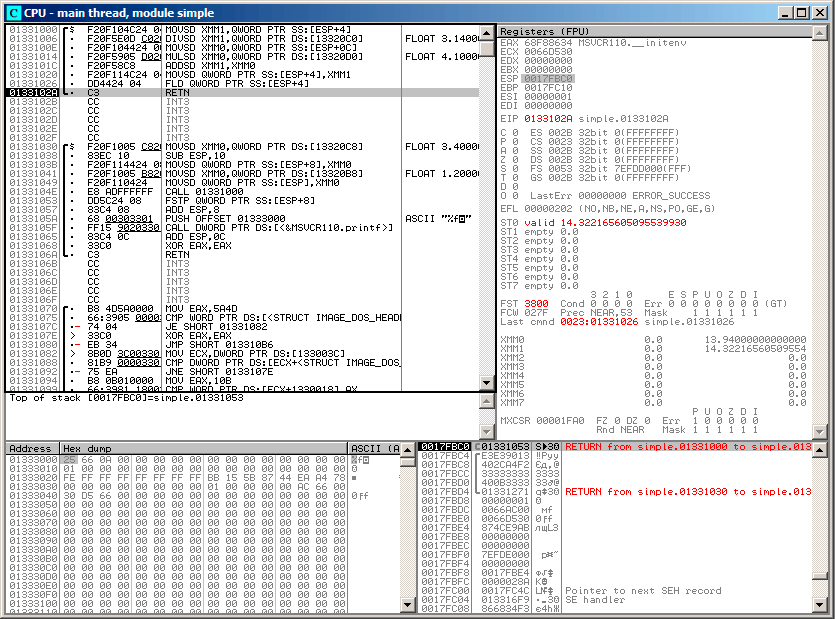
\includegraphics[scale=\FigScale]{patterns/205_floating_SIMD/simple_olly5.png}
\caption{\olly: \FLD \RU{оставляет результат ф-ции в}\EN{left function result in} \ST{0}}
\label{fig:FPU_SIMD_simple_olly5}
\end{figure}

\RU{Видно, что \olly показывает XMM-регистры как пары чисел в формате \Tdouble,
но используется только \IT{младшая} часть.}
\EN{We see that \olly shows the XMM registers as pairs of \Tdouble numbers,
but only the \IT{lower} part is used.}
\RU{Должно быть, \olly показывает их именно так, потому что сейчас исполняются SSE2-инструкции
с суффиксом \TT{-SD}.}
\EN{Apparently, \olly shows them in that format because the SSE2 instructions (suffixed with \TT{-SD}) 
are executed right now.}
\RU{Но конечно же, можно переключить отображение значений в регистрах и посмотреть содержимое
как 4 \Tfloat{}-числа или просто как 16 байт.}
\EN{But of course, it's possible to switch the register format and to see their contents as
4 \Tfloat{}-numbers or just as 16 bytes.}
\fi

\clearpage
\section{\RU{Передача чисел с плавающей запятой в аргументах}\EN{Passing floating point number via arguments}}

\lstinputlisting{patterns/12_FPU/2_passing_floats/pow.c}

\RU{Они передаются в младших половинах регистров}\EN{They are passed in the lower halves
of the} \XMM{0}-\XMM{3}\EN{ registers}.

\lstinputlisting[caption=\Optimizing MSVC 2012 x64]{patterns/205_floating_SIMD/pow_MSVC_2012_x64_Ox.asm}

\index{x86!\Instructions!MOVSD}
\index{x86!\Instructions!MOVSDX}
\RU{Инструкции}\EN{There is no} \TT{MOVSDX} \RU{нет в документации от}\EN{instruction in} 
Intel \cite{Intel} \AndENRU AMD \cite{AMD}\EN{ manuals}, 
\RU{там она называется просто}\EN{there it is called just} \TT{MOVSD}.
\RU{Таким образом, в процессорах x86 две инструкции с одинаковым именем}\EN{So there are two instructions
sharing the same name in x86} (\RU{о второй}\EN{about the other see}: \myref{REP_MOVSx}).
\RU{Возможно, в Microsoft решили избежать
путаницы и переименовали инструкцию в}\EN{Apparently, Microsoft developers wanted to get rid of the mess,
so they renamed it to} \TT{MOVSDX}.
\RU{Она просто загружает значение в младшую половину XMM-регистра}\EN{It just loads a value into
the lower half of a XMM register}.

\RU{Ф-ция }\TT{pow()} \RU{берет аргументы из}\EN{takes arguments from} \XMM{0} \AndENRU \XMM{1}, 
\RU{и возвращает результат в}\EN{and returns result in} \XMM{0}.
\RU{Далее он перекладывается в}\EN{It is then moved to} \RDX \ForENRU \printf. 
\RU{Почему}\EN{Why}? 
\RU{Честно говоря, не знаю, может быть, это потому что}\EN{Honestly speaking, I don't know, maybe because} 
\printf\EMDASH{}\RU{ф-ция с переменным количеством аргументов}\EN{is a variable arguments function}?

\lstinputlisting[caption=\Optimizing GCC 4.4.6 x64]{patterns/205_floating_SIMD/pow_GCC446_x64_O3.s.\LANG}

GCC \RU{работает понятнее}\EN{generates clearer output}. 
\RU{Значение для}\EN{The value for} \printf \RU{передается в}\EN{is passed in} \XMM{0}. 
\RU{Кстати, вот тот случай, когда в}\EN{By the way, here is a case when 1 is written into} \EAX
\ForENRU \printf \RU{записывается 1 --- это значит, что будет передан один аргумент в векторных регистрах, 
так того требует стандарт}\EN{---this means that one argument will be passed in vector registers,
just as the standard requires} \cite{SysVABI}.

\section{\RU{Пример с сравнением}\EN{Comparison example}}

\lstinputlisting{patterns/12_FPU/3_comparison/d_max.c}

\subsection{x64}

\lstinputlisting[caption=\Optimizing MSVC 2012 x64]{patterns/205_floating_SIMD/d_max_MSVC_2012_x64_Ox.asm}

\Optimizing MSVC \RU{генерирует очень понятный код}\EN{generates a code very easy to understand}.

\index{x86!\Instructions!COMISD}
\RU{Инструкция }\TT{COMISD} \RU{это}\EN{is} ``Compare Scalar Ordered Double-Precision Floating-Point 
Values and Set EFLAGS''. \RU{Собственно, это она и делает}\EN{Essentially, that is what it does}.\\
\\
\NonOptimizing MSVC \RU{генерирует более избыточно, но тоже всё понятно}\EN{generates more redundant code,
but it is still not hard to understand}:

\lstinputlisting[caption=MSVC 2012 x64]{patterns/205_floating_SIMD/d_max_MSVC_2012_x64.asm}

\index{x86!\Instructions!MAXSD}
\RU{А вот}\EN{However,} GCC 4.4.6 \RU{дошел в оптимизации дальше и применил инструкцию}
\EN{did more optimizations and used the} \TT{MAXSD} (``Return Maximum Scalar 
Double-Precision Floating-Point Value'')\RU{, которая просто выбирает максимальное значение}\EN{ instruction,
which just choose the maximum value}!

\lstinputlisting[caption=\Optimizing GCC 4.4.6 x64]{patterns/205_floating_SIMD/d_max_GCC446_x64_O3.s}

\clearpage
\subsection{x86}

\RU{Скомпилируем этот пример в MSVC 2012 с включенной оптимизацией:}
\EN{Let's compile this example in MSVC 2012 with optimization turned on:}

\lstinputlisting[caption=\Optimizing MSVC 2012 x86]{patterns/205_floating_SIMD/d_max_MSVC_2012_x86_Ox.asm}

\RU{Всё то же самое, только значения}\EN{Almost the same, but the values of} $a$ \AndENRU $b$ 
\RU{берутся из стека, а результат функции оставляется в}\EN{are taken from the stack and the function result 
is left in} \ST{0}.

\ifdefined\IncludeOlly
\RU{Если загрузить этот пример в}\EN{If we load this example in} \olly, 
\RU{увидим, как инструкция}\EN{we will see how the} \TT{COMISD} \RU{сравнивает значения и устанавливает/сбрасывает
флаги}\EN{instruction compares values and sets/clears the} \CF \AndENRU \PF\EN{ flags}:

\begin{figure}[H]
\centering
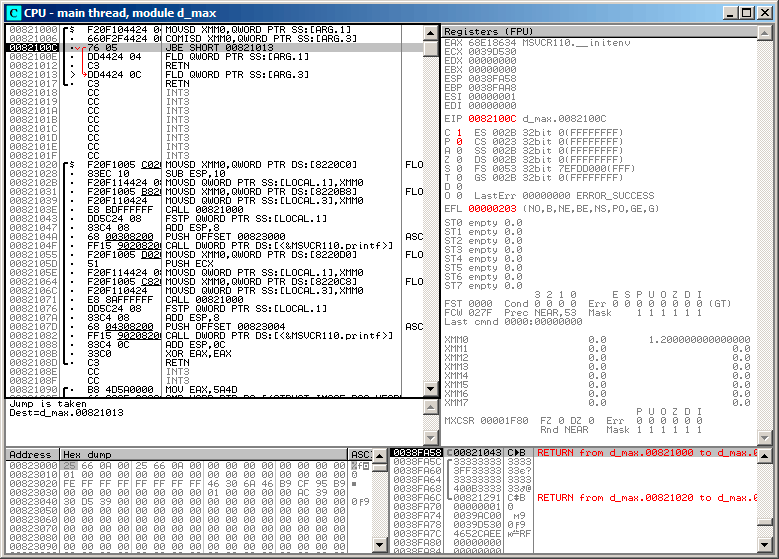
\includegraphics[scale=\FigScale]{patterns/205_floating_SIMD/d_max_olly.png}
\caption{\olly: \TT{COMISD} \RU{изменила флаги}\EN{changed} \CF \AndENRU \PF\EN{ flags}}
\label{fig:FPU_SIMD_d_max_olly}
\end{figure}
\fi

\section{\RU{Вычисление машинного эпсилона}\EN{Calculating machine epsilon}: x64 \AndENRU SIMD}
\label{machine_epsilon_x64_and_SIMD}

\RU{Вернемся к примеру ``вычисление машинного эпсилона'' для \Tdouble \lstref{machine_epsilon_double_c}.}
\EN{Let's revisit the ``calculating machine epsilon'' example for \Tdouble \lstref{machine_epsilon_double_c}.}

\RU{Теперь скомпилируем его для x64}\EN{Now we compile it for x64}:

\lstinputlisting[caption=\Optimizing MSVC 2012 x64]{patterns/205_floating_SIMD/epsilon_double_MSVC_2012_x64_Ox.asm}

\RU{Нет способа прибавить 1 к значению в 128-битном XMM-регистре, так что его нужно в начале поместить в память.}
\EN{There is no way to add 1 to a value in 128-bit XMM register, so it must be placed into memory.}

\RU{Впрочем, есть инструкция ADDSD (\IT{Add Scalar Double-Precision Floating-Point Values}),
которая может прибавить значение к младшей 64-битной части XMM-регистра игнорируя старшую половину,
но наверное MSVC 2012 пока недостаточно хорош для этого}
\EN{There is, however, the ADDSD instruction (\IT{Add Scalar Double-Precision Floating-Point Values}) 
which can add a value to the lowest 64-bit half of a XMM register while ignoring the higher one, 
but MSVC 2012 probably is not that good yet}
\footnote{\RU{В качестве упражнения, вы можете попробовать переработать этот код, чтобы избавиться 
от использования локального стека}\EN{As an exercise, you may try to rework this code to 
eliminate the usage of the local stack}.}.

\RU{Так или иначе, значение затем перезагружается в XMM-регистр и происходит вычитание.}
\EN{Nevertheless, the value is then reloaded to a XMM register and subtraction occurs.}
SUBSD \RU{это}\EN{is} ``Subtract Scalar Double-Precision Floating-Point Values'', 
\RU{т.е., операция производится над младшей 64-битной частью 128-битного XMM-регистра}
\EN{i.e., it operates on the lower 64-bit part of 128-bit XMM register}.
\RU{Результат возвращается в регистре XMM0}\EN{The result is returned in the XMM0 register}.

\section{\RU{И снова пример генератора случайных чисел}\EN{Pseudo-random number generator example revisited}}
\label{FPU_PRNG_SIMD}

\RU{Вернемся к примеру \q{пример генератора случайных чисел} \lstref{FPU_PRNG}.}
\EN{Let's revisit \q{pseudo-random number generator example} example \lstref{FPU_PRNG}.}

\RU{Если скомпилировать это в MSVC 2012, компилятор будет использовать SIMD-инструкции для FPU.}
\EN{If we compile this in MSVC 2012, it will use the SIMD instructions for the FPU.}

\lstinputlisting[caption=\Optimizing MSVC 2012]{patterns/205_floating_SIMD/FPU_PRNG/MSVC2012_Ox_Ob0.asm.\LANG}

% FIXME1 rewrite!
\RU{У всех инструкций суффикс -SS, это означает \q{Scalar Single}.}
\EN{All instructions have the -SS suffix, which stands for \q{Scalar Single}.}
\RU{\q{Scalar} означает что только одно значение хранится в регистре.}
\EN{\q{Scalar} implies that only one value is stored in the register.}
\RU{\q{Single} означает что это тип \Tfloat.}
\EN{\q{Single} stands for \Tfloat data type.}


\section{\RU{Итог}\EN{Summary}}

\RU{Во всех приведенных примерах, в XMM-регистрах используется только младшая половина регистра, там
хранится значение в формате IEEE 754}\EN{Only the lower half of XMM registers is used in all examples here, 
to store number in IEEE 754 format}.

\RU{Собственно, все инструкции с суффиксом}\EN{Essentially, all instructions prefixed by} 
\TT{-SD} (``Scalar Double-Precision'')\EMDASH{}\RU{это инструкции для работы с числами с плавающей 
запятой в формате IEEE 754, 
хранящиеся в младшей 64-битной половине XMM-регистра}\EN{are instructions working with floating point numbers
in IEEE 754 format, stored in the lower 64-bit half of a XMM register}.

\RU{Всё удобнее чем это было в FPU, видимо, сказывается тот факт, что расширения 
SIMD развивались не так хаотично как FPU в прошлом.}
\EN{And it is easier than in the FPU, probably because the SIMD extensions 
were evolved in a less chaotic way than the FPU ones in the past.}
\RU{Стековая модель регистров не используется}\EN{The stack register model is not used}.

\index{x86!\Instructions!ADDSS}
\index{x86!\Instructions!MOVSS}
\index{x86!\Instructions!COMISS}
% TODO: do this!
\RU{Если вы попробуете заменить в этих примерах}\EN{If you would try to replace} \Tdouble \RU{на}\EN{with} \Tfloat
\RU{, то инструкции будут использоваться те же,
только с суффиксом}\EN{in these examples, the same instructions will be used, but prefixed with} \TT{-SS} 
(``Scalar Single-Precision''), \RU{например}\EN{for example}, \TT{MOVSS}, \TT{COMISS}, \TT{ADDSS}, \RU{и т.д.}\EN{etc.}

``Scalar'' \RU{означает что SIMD-регистр будет хранить только одно значение, вместо нескольких}\EN{means that
the SIMD register will contain only one value instead of several}.
\RU{Инструкции, работающие с несколькими значениями в регистре одновременно, имеют ``Packed'' в названии}
\EN{Instructions working with several values in a register simultaneously have ``Packed'' in their name}.

\RU{Нужно также обратить внимание, что SSE2-инструкции работают с 64-битными числами (\Tdouble) в формате IEEE 754,
в то время как внутреннее представление в FPU --- 80-битные числа.}
\EN{Needless to say, the SSE2 instructions work with 64-bit IEEE 754 numbers (\Tdouble),
while the internal representation of the floating-point numbers in FPU is 80-bit numbers.}
\RU{Поэтому ошибок округления (\IT{round-off error}) в FPU может быть меньше чем в SSE2,
как следствие, можно сказать, работа с FPU может давать более точные результаты вычислений.}
\EN{Hence, the FPU may produce less round-off errors and as a consequence, FPU may give more precise
calculation results.}

\fi
\ifdefined\IncludeARM
\chapter{\EN{More about ARM}\RU{Еще немного об ARM}}

\section{\RU{Знак номера}\EN{Number sign} (\#) \RU{перед числом}\EN{before number}}

\RU{Компилятор Keil, \IDA и objdump предваряет все числа знаком номера (``\#''), например:}
\EN{The Keil compiler, \IDA and objdump precede all numbers with the ``\#'' number sign, for example:}
\lstref{Keil_number_sign}.
\RU{Но когда GCC 4.9 выдает результат на языке ассемблера, он так не делает, например:}
\EN{But when GCC 4.9 generates assembly language output, it doesn't, for example: }
\lstref{GCC_no_number_sign}.

\RU{Так что листинги для ARM в этой книге в каком-то смысле перемешаны.}
\EN{The ARM listings in this book are somewhat mixed.}

\RU{Я не знаю, как правильнее.}\EN{I'm not sure which method is right.}
\RU{Должно быть, всякий должен придерживаться тех правил, которые приняты в той среде,
в которой он работает.}
\EN{Supposedly, one should obey the rules accepted in environment he/she works in.}

% sections
\section{\RU{Режимы адресации}\EN{Adressing modes}}
\index{ARM!\RU{Режимы адресации}\EN{Adressing modes}}
\label{ARM_postindex_vs_preindex}
\index{\CLanguageElements!\PostIncrement}
\index{\CLanguageElements!\PostDecrement}
\index{\CLanguageElements!\PreIncrement}
\index{\CLanguageElements!\PreDecrement}

\EN{This instruction is possible in ARM64:}
\RU{В ARM64 возможна такая инструкция:}

\index{ARM!\Instructions!LDR}
\begin{lstlisting}
ldr	x0, [x29,24]
\end{lstlisting}

\EN{This mean, add 24 to value in X29 and load value at this address.}
\RU{И это означает прибавить 24 к значению в X29 и загрузить значение по этому адресу.}
\RU{Обратите внимание что 24 внутри скобок.}
\EN{Please note that 24 is inside brackets.}
\EN{Meaning is different if number is outside brackets:}
\RU{А если снаружи скобок, то весь смысл меняется:}

\begin{lstlisting}
ldr	w4, [x1],28
\end{lstlisting}

\RU{Это означает, загрузить значение по адресу в X1, затем прибавить 28 к X1.}
\EN{This mean, load a value at address in X1, then add 28 to X1.}

\index{PDP-11}
\RU{ARM позволяет прибавлять некоторую константу к адресу, с которого происходит загрузка, либо вычитать.}
\EN{ARM allows to add some constant to the address used for loading, or to subtract.}
\RU{Причем, позволяет это делать до загрузки или после.}
\EN{And it's possible both after loading and before.}

\RU{Такого режима адресации в x86 нет, но он есть в некоторых других процессорах, даже на PDP-11.}
\EN{There is no such addressing mode in x86, but it is present in some other processors, even on PDP-11.}
\RU{Существует байка, что режимы пре-инкремента, пост-инкремента, 
пре-декремента и пост-декремента адреса в PDP-11}
\EN{There is a legend the pre-increment, post-increment, pre-decrement and post-decrement modes in PDP-11},
\RU{были ``виновны'' в появлении таких конструкций языка Си (который разрабатывался на PDP-11) как}
\EN{were ``guilty'' in appearance such C language (which developed on PDP-11) constructs as}
*ptr++, *++ptr, *ptr-{}-, *-{}-ptr. 
\RU{Кстати, это является трудно запоминаемой особенностью в Си.}
\EN{By the way, this is one of hard to memorize C feature.}
\RU{Дела обстоят так:}\EN{This is how it is:}

% FIXME: add ARM assembly...
\begin{center}
\begin{tabular}{ | l | l | l | l | }
\hline
\headercolor{} \RU{термин в Си}\EN{C term} & 
\headercolor{} \RU{термин в ARM}\EN{ARM term} & 
\headercolor{} \RU{выражение Си}\EN{C statement} & 
\headercolor{} \RU{как это работает}\EN{how it works} \\
\hline
\PostIncrement & 
post-indexed addressing & 
\TT{*ptr++} & 
\RU{использовать значение \TT{*ptr}}\EN{use \TT{*ptr} value}, \\
& & & \RU{затем инкремент указателя \TT{ptr}}\EN{then \gls{increment} \TT{ptr} pointer} \\
\hline
\PostDecrement & 
post-indexed addressing & 
\TT{*ptr-{}-} & 
\RU{использовать значение \TT{*ptr}}\EN{use \TT{*ptr} value}, \\
& & & \RU{затем \glslink{decrement}{декремент} указателя \TT{ptr}}\EN{then \gls{decrement} \TT{ptr} pointer} \\
\hline
\PreIncrement & 
pre-indexed addressing & 
\TT{*++ptr} & 
\RU{инкремент указателя \TT{ptr}}\EN{\gls{increment} \TT{ptr} pointer}, \\
& & & \RU{затем использовать значение \TT{*ptr}}\EN{then use \TT{*ptr} value} \\
\hline
\PreDecrement & 
pre-indexed addressing & 
\TT{*-{}-ptr} & 
\RU{\glslink{decrement}{декремент} указателя \TT{ptr}}\EN{\gls{decrement} \TT{ptr} pointer}, \\
& & & \RU{затем использовать значение \TT{*ptr}}\EN{then use \TT{*ptr} value} \\
\hline
\end{tabular}
\end{center}

Pre-indexing \EN{marked as exclamation mark in ARM assembly language}\RU{маркируется как 
восклицательный знак в ассемблере ARM}.
\RU{Для примера, смотрите строку 2 в}\EN{For example, see line 2 in} \lstref{hw_ARM64_GCC}.

\RU{Деннис Ритчи (один из создателей ЯП Си) указывал, что, это, вероятно, придумал Кен Томпсон 
(еще один создатель Си),
потому что подобная возможность процессора имелась еще в PDP-7}
\EN{Dennis Ritchie (one of C language creators) mentioned that it is, probably, was invented by Ken Thompson
(another C creator) because this processor feature was present in PDP-7}
\cite{Ritchie:1986}\cite{Ritchie:1993:DCL:155360.155580}.
\RU{Таким образом, компиляторы с ЯП Си на тот процессор, где это есть, могут использовать это.}
\EN{Thus, C language compilers may use it, if it is present on target processor.}

\RU{Всё это очень удобно для работы с массивами.}
\EN{That's very convenient for array processings.}

\section{\RU{Загрузка констант в регистр}\EN{Loading constants into register}}

\subsection{\RU{32-битный}\EN{32-bit} ARM}
\label{ARM_big_constants_loading}

\RU{Как мы уже знаем, все инструкции имеют длину в 4 байта в режиме ARM и 2 байта в режиме Thumb.}
\EN{Aa we already know, all instructions has length of 4 bytes in ARM mode and 2 bytes in Thumb mode.}
\RU{Как в таком случае записать в регистр 32-битное число, если его невозможно закодировать
внутри одной инструкции?}
\EN{How to load 32-bit value into register, if it's not possible to encode it inside one instruction?}

\RU{Попробуем}\EN{Let's try}:

\begin{lstlisting}
unsigned int f()
{
	return 0x12345678;
};
\end{lstlisting}

\begin{lstlisting}[caption=GCC 4.6.3 -O3 \ARMMode]
f:
        ldr     r0, .L2
        bx      lr
.L2:
        .word   305419896 ; 0x12345678
\end{lstlisting}

\RU{Т.е., значение \TT{0x12345678} просто записано в памяти отдельно и загружается, если нужно.}
\EN{So, the \TT{0x12345678} value just stored aside in memory and loads if it needs.}
\RU{Но можно обойтись и без дополнительного обращения к памяти.}
\EN{But it's possible to get rid of additional memory access.}

\begin{lstlisting}[caption=GCC 4.6.3 -O3 -march{=}armv7-a (\ARMMode)]
movw    r0, #22136      ; 0x5678
movt    r0, #4660       ; 0x1234
bx      lr
\end{lstlisting}

\RU{Видно что число загружается в регистр по частям, в начале младшая часть 
(при помощи инструкции MOVW), затем старшая (при помощи MOVT).}
\EN{We see that value is loaded into register by parts, lower part first (using MOVW instruction), 
then higher (using MOVT).}

\RU{Следовательно, нужно 2 инструкции в режиме ARM, чтобы записать 32-битное число в регистр.}
\EN{It means, 2 instructions are necessary in ARM mode for loading 32-bit value into register.}
\RU{Это не так уж и страшно, потому что в реальном коде не так уж и много констант (кроме 0 и 1).}
\EN{It's not a real problem, because in fact there are not much constants in the real code (except of 0 and 1).}
\RU{Значит ли это, что это исполняется медленнее чем одна инструкция, как две инструкции?}
\EN{Does it mean it executes slower then one instruction, as two instructions?}
\RU{Врядли, наверняка современные процессоры ARM наверняка умеют распознавать такие 
последовательности и исполнять их быстро.}
\EN{Doubtfully. Most likely, modern ARM processors are able to detect such sequences and execute
them fast.}

\RU{А \IDA легко распознает подобные паттерны в коде и дизассемблирует эту ф-цию как:}
\EN{On the other hand, \IDA is able to detect such patterns in the code and disassembles this function as:}

\begin{lstlisting}
MOV    R0, 0x12345678
BX     LR
\end{lstlisting}

\subsection{ARM64}

\begin{lstlisting}
uint64_t f()
{
	return 0x12345678ABCDEF01;
};
\end{lstlisting}

\begin{lstlisting}[caption=GCC 4.9.1 -O3]
mov	x0, 61185   ; 0xef01
movk	x0, 0xabcd, lsl 16
movk	x0, 0x5678, lsl 32
movk	x0, 0x1234, lsl 48
ret
\end{lstlisting}

\index{ARM!\Instructions!MOVK}
\TT{MOVK} \RU{означает}\EN{means} ``MOV Keep'', \RU{т.е., она записывает 16-битное значение в регистр, не трогая
при этом остальные биты.}\EN{i.e., it writes 16-bit value into register, not touching other bits at the same 
time.}
\index{ARM!Optional operators!LSL}
\RU{Суффикс }\TT{LSL} \RU{сдвигает значение в каждом случае влево на 16, 32 и 48 бит. Сдвиг происходит
перед загрузкой.}\EN{suffix shifts value left by 16, 32 and 48 bits at each step. Shifting done before loading.}
\RU{Таким образом, нужно 4 инструкции, чтобы записать в регистр 64-битное значение.}
\EN{This means, 4 instructions are necessary to load 64-bit value into register.}

\subsubsection{\RU{Записать числа с плавающей точкой в регистр}\EN{Storing floating number into register}}

\RU{Некоторые числа можно записывать в D-регистр при помощи только одной инструкции.}
\EN{It's possible to store a floating number into D-register using only one instruction.}

\RU{Например}\EN{For example}:

\begin{lstlisting}
double a()
{
	return 1.5;
};
\end{lstlisting}

\begin{lstlisting}[caption=GCC 4.9.1 -O3 + objdump]
0000000000000000 <a>:
   0:   1e6f1000        fmov    d0, #1.500000000000000000e+000
   4:   d65f03c0        ret
\end{lstlisting}

\RU{Число $1.5$ действительно было закодировано в 32-битной инструкции.}
\EN{$1.5$ number was indeed encoded in 32-bit instruction.}
\RU{Но как}\EN{But how}?
\index{ARM!\Instructions!FMOV}
\RU{В ARM64, инструкцию \TT{FMOV} есть 8 бит для кодирования некоторых чисел с плавающей запятой.}
\EN{In ARM64, there are 8 bits in \TT{FMOV} instruction for encoding some float point numbers.}
\RU{В \cite{ARM64ref} алгоритм называется \TT{VFPExpandImm()}.}
\EN{The algorithm is called \TT{VFPExpandImm()} in \cite{ARM64ref}.}
\index{minifloat}
\EN{This is also called}\RU{Это также называется} \IT{minifloat}\footnote{\url{http://go.yurichev.com/17139}}.
\RU{Я попробовал разные: $30.0$ и $31.0$ компилятору удается закодировать, а $32.0$ уже нет, для него
приходится выделять 8 байт в памяти и записать его там в формате IEEE 754:}
\EN{I tried different: compiler is able to encode $30.0$ and $31.0$, but it couldn't encode $32.0$,
an 8 bytes should be allocated to this number in IEEE 754 format:}

\begin{lstlisting}
double a()
{
	return 32;
};
\end{lstlisting}

\begin{lstlisting}[caption=GCC 4.9.1 -O3]
a:
	ldr	d0, .LC0
	ret
.LC0:
	.word	0
	.word	1077936128
\end{lstlisting}

\newcommand{\ARMELF}{[\IT{ELF for the ARM 64-bit Architecture (AArch64)}, (2013)]\footnote{\AlsoAvailableAs \url{http://go.yurichev.com/17288}}}

\section{\RU{Релоки}\EN{Relocs} \InENRU ARM64}
\label{ARM64_relocs}

\RU{Как известно, в ARM64 инструкции 4-байтные, так что записать длинное число в регистр одной инструкцией нельзя.}
\EN{As we know, there are 4-byte instructions in ARM64, so it is impossible to write a large number into a register
using a single instruction.}
\RU{Тем не менее, файл может быть загружен по произвольному адресу в памяти, для этого релоки и нужны.}
\EN{Nevertheless, an executable image can be loaded at any random address in memory, so that's why relocs exists.}
\RU{Больше о них (в связи с Win32 PE)}\EN{Read more about them (in relation to Win32 PE)}: \myref{subsec:relocs}.

\myindex{ARM!\Instructions!ADRP/ADD pair}
\RU{В ARM64 принят следующий метод: адрес формируется при помощи пары инструкций: \TT{ADRP} и \ADD.}
\EN{The address is formed using the \TT{ADRP} and \ADD instruction pair in ARM64.}
\RU{Первая загружает в регистр адрес 4KiB-страницы, а вторая прибавляет остаток.}
\EN{The first loads a 4KiB-page address and the second one adds the remainder.}
\RU{Скомпилируем пример из}\EN{Let's compile the example from} \q{\HelloWorldSectionName} 
(\lstref{hw_c}) \InENRU GCC (Linaro) 4.9 \RU{под}\EN{under} win32:

\begin{lstlisting}[caption=GCC (Linaro) 4.9 \AndENRU objdump \EN{of object file}\RU{объектного файла}]
...>aarch64-linux-gnu-gcc.exe hw.c -c

...>aarch64-linux-gnu-objdump.exe -d hw.o

...

0000000000000000 <main>:
   0:   a9bf7bfd        stp     x29, x30, [sp,#-16]!
   4:   910003fd        mov     x29, sp
   8:   90000000        adrp    x0, 0 <main>
   c:   91000000        add     x0, x0, #0x0
  10:   94000000        bl      0 <printf>
  14:   52800000        mov     w0, #0x0                        // #0
  18:   a8c17bfd        ldp     x29, x30, [sp],#16
  1c:   d65f03c0        ret

...>aarch64-linux-gnu-objdump.exe -r hw.o

...

RELOCATION RECORDS FOR [.text]:
OFFSET           TYPE              VALUE
0000000000000008 R_AARCH64_ADR_PREL_PG_HI21  .rodata
000000000000000c R_AARCH64_ADD_ABS_LO12_NC  .rodata
0000000000000010 R_AARCH64_CALL26  printf
\end{lstlisting}

\RU{Итак, в этом объектом файле три релока.}
\EN{So there are 3 relocs in this object file.}

\begin{itemize}
\item 
\RU{Самый первый берет адрес страницы, отсекает младшие 12 бит и записывает оставшиеся старшие 21
в битовые поля инструкции \TT{ADRP}. Это потому что младшие 12 бит кодировать не нужно,
и в ADRP выделено место только для 21 бит.}
\EN{The first one takes the page address, cuts the lowest 12 bits and writes the remaining high 21 bits
to the \TT{ADRP} instruction's bit fields. This is because we don't need to encode the low 12 bits,
and the ADRP instruction has space only for 21 bits.}

\item \RU{Второй ---- 12 бит адреса, относительного от начала страницы, в поля инструкции \ADD.}
\EN{The second one puts the 12 bits of the address relative to the page start into the \ADD instruction's bit fields.}

\item \RU{Последний, 26-битный, накладывается на инструкцию по адресу \TT{0x10}, где переход на функцию \printf.}
\EN{The last, 26-bit one, is applied to the instruction at address \TT{0x10} where the 
jump to the \printf function is.}
\RU{Все адреса инструкций в ARM64 (да и в ARM в режиме ARM) имеют нули в двух младших битах
(потому что все инструкции имеют размер в 4 байта),
так что нужно кодировать только старшие 26 бит из 28-битного адресного пространства ($\pm 128$MB).}
\EN{All ARM64 (and in ARM in ARM mode) instruction addresses have zeroes in the two lowest bits
(because all instructions have a size of 4 bytes),
so one need to encode only the highest 26 bits of 28-bit address space ($\pm 128$MB).}

\end{itemize}

\RU{В слинкованном исполняемом файле релоков в этих местах нет: потому что там уже точно известно, 
где будет находится строка \q{Hello!}, и в какой странице, а также известен адрес функции \puts.}
\EN{There are no such relocs in the executable file: because it's known where the \q{Hello!} string
is located, in which page, and the address of \puts is also known.}
\RU{И поэтому там, в инструкциях \TT{ADRP}, \ADD и \TT{BL}, уже проставлены нужные значения 
(их проставил линкер во время компоновки):}
\EN{So there are values set already in the \TT{ADRP}, \ADD and \TT{BL} instructions
(the linker has written them while linking):}

\begin{lstlisting}[caption=objdump \EN{of executable file}\RU{исполняемого файла}]
0000000000400590 <main>:
  400590:       a9bf7bfd        stp     x29, x30, [sp,#-16]!
  400594:       910003fd        mov     x29, sp
  400598:       90000000        adrp    x0, 400000 <_init-0x3b8>
  40059c:       91192000        add     x0, x0, #0x648
  4005a0:       97ffffa0        bl      400420 <puts@plt>
  4005a4:       52800000        mov     w0, #0x0                        // #0
  4005a8:       a8c17bfd        ldp     x29, x30, [sp],#16
  4005ac:       d65f03c0        ret

...

Contents of section .rodata:
 400640 01000200 00000000 48656c6c 6f210000  ........Hello!..
\end{lstlisting}

\myindex{ARM!\Instructions!BL}

\ifdefined\ENGLISH{}
As an example, let's try to disassemble the BL instruction manually.\\
\TT{0x97ffffa0} is $10010111111111111111111110100000b$.
According to [\ARMSixFourRef C5.6.26], \IT{imm26} is the last 26 bits: $imm26 = 11111111111111111110100000$.
It is \TT{0x3FFFFA0}, but the \ac{MSB} is 1, 
so the number is negative, and we can convert it manually to convenient form for us.
By the rules of negation (\myref{sec:signednumbers:negation}), just invert all bits: (it is \TT{1011111=0x5F}), and add 1 (\TT{0x5F+1=0x60}).
So the number in signed form is \TT{-0x60}.
Let's multiplicate \TT{-0x60} by 4 (because address stored in opcode is divided by 4): it is \TT{-0x180}.
Now let's calculate destination address: \TT{0x4005a0} + (\TT{-0x180}) = \TT{0x400420} 
(please note: we consider the address of the BL instruction, not the current value of \ac{PC}, which may be different!).
So the destination address is \TT{0x400420}.\\
\\
More about ARM64-related relocs: \ARMELF.
\fi

\ifdefined\RUSSIAN{}
В качестве примера, попробуем дизассемблировать инструкцию BL вручную.\\
\TT{0x97ffffa0} это $10010111111111111111111110100000b$.
В соответствии с [\ARMSixFourRef C5.6.26], \IT{imm26} это последние 26 бит: $imm26 = 11111111111111111110100000$.
Это \TT{0x3FFFFA0}, но \ac{MSB} это 1, 
так что число отрицательное, мы можем вручную его конвертировать в удобный для нас вид.
По правилам изменения знака (\myref{sec:signednumbers:negation}), просто инвертируем все биты: (\TT{1011111=0x5F}) и прибавляем 1 (\TT{0x5F+1=0x60}).
Так что число в знаковом виде: \TT{-0x60}.
Умножим \TT{-0x60} на 4 (потому что адрес записанный в опкоде разделен на 4): это \TT{-0x180}.
Теперь вычисляем адрес назначения: \TT{0x4005a0} + (\TT{-0x180}) = \TT{0x400420} 
(пожалуйста заметьте: мы берем адрес инструкции BL, а не текущее значение \ac{PC}, которое может быть другим!).
Так что адрес в итоге \TT{0x400420}.\\
\\
Больше о релоках связанных с ARM64: \ARMELF.
\fi


\fi
\ifdefined\IncludeMIPS
\chapter{\EN{MIPS-specific details}\RU{Кое-что специфичное для MIPS}}

% sections
\subsection{\RU{Загрузка констант в регистр}\EN{Loading constants into register}}
\label{MIPS_big_constants}

\begin{lstlisting}
unsigned int f()
{
	return 0x12345678;
};
\end{lstlisting}

\RU{В MIPS, так же как и в ARM, все инструкции имеют размер 32 бита, так что невозможно
закодировать 32-битную константу в инструкцию.}
\EN{All instructions in MIPS, just like ARM, have a of 32-bit, so it's not possible to
embed a 32-bit constant into one instruction.}
\myindex{MIPS!\Instructions!LI}
\myindex{MIPS!\Instructions!ORI}
\RU{Так что это транслируется в две инструкции:
первая загружает старшую часть 32-битного числа и вторая применяет операцию \q{ИЛИ},
эффект от которой в том, что она просто выставляет младшие 16 бит целевого регистра:}
\EN{So this translates to at least two instructions: 
the first loads the high part of the 32-bit number and the second
one applies an OR operation, which effectively sets the low 16-bit part of the target register:}

\begin{lstlisting}[caption=GCC 4.4.5 -O3 (\assemblyOutput)]
        li      $2,305397760                    # 0x12340000
        j       $31
        ori     $2,$2,0x5678 ; branch delay slot
\end{lstlisting}

\IDA \RU{знает о таких часто встречающихся последовательностях, так что для удобства, 
она показывает последнюю инструкцию ORI как псевдоинструкцию LI, 
которая якобы загружает полное 32-битное значение в регистр \$V0.}
\EN{is fully aware of such frequently encountered code patterns, 
so, for convenience it shows the last ORI instruction as the LI pseudoinstruction,
which allegedly loads a full 32-bit number into the \$V0 register.}

\myindex{MIPS!\Instructions!LUI}

\begin{lstlisting}[caption=GCC 4.4.5 -O3 (IDA)]
         lui     $v0, 0x1234
         jr      $ra
         li      $v0, 0x12345678 ; branch delay slot
\end{lstlisting}

\RU{В выводе на ассемблере от GCC есть псевдоинструкция LUI, но на самом деле, 
там LUI (\q{Load Upper Immediate}), загружающая 16-битное значение в старшую часть регистра.}
\EN{The GCC assembly output has the LI pseudoinstruction, but in fact, LUI (\q{Load Upper Imeddiate}) is there,
which stores a 16-bit value into the high part of the register.}


\section{\RU{Книги и прочие материалы о MIPS}\EN{Further reading about MIPS}}

\cite{MIPSRun}.

\fi

\chapter{\Cpp}

\section{\IFRU{Классы}{Classes}}
% subsections here:
\subsection{\IFRU{Классы}{Classes}}

\subsubsection{\IFRU{Простой пример}{Simple example}}

\IFRU{Внутреннее представление классов в Си++ почти такое же как и представление структур.}
{Internally, C++ classes representation is almost the same as structures representation.}

\IFRU{Давайте попробуем простой пример с двумя переменными, двумя конструкторами и одним методом:}
{Let's try an example with two variables, two constructors and one method:}

\lstinputlisting{cpp/classes/16_1.cpp}

\IFRU{Вот как выглядит \main на ассемблере:}{Here is how \main function looks like translated 
into assembly language:}

\lstinputlisting{cpp/classes/16_1_msvc.asm}

\IFRU{Вот что происходит. 
Под каждый экземпляр класса \IT{c} выделяется по 8 байт, столько же, сколько нужно 
для хранения двух переменных.}
{So what's going on.
For each object (instance of class \IT{c}) 8 bytes allocated,
that is exactly size of 2 variables storage.}

\IFRU{Для \IT{c1} вызывается конструктор по умолчанию без аргументов \TT{??0c@@QAE@XZ}. 
Для \IT{c2} вызывается другой конструктор \TT{??0c@@QAE@HH@Z} и передаются два числа в качестве аргументов.}
{For \IT{c1} a default argumentless constructor \TT{??0c@@QAE@XZ} is called.
For \IT{c2} another constructor \TT{??0c@@QAE@HH@Z} is called and two numbers are passed as arguments.}

\index{thiscall}
\label{thiscall}
\index{x86!\Registers!ECX}
\IFRU{А указатель на объект (\IT{this} в терминологии Си++) передается в регистре \ECX. 
Это называется thiscall~(\ref{thiscall}) ~--- метод передачи указателя на объект.}
{A pointer to object (\IT{this} in C++ terminology) is passed in the \ECX register.
This is called thiscall~(\ref{thiscall})~---a pointer to object passing method.}

\IFRU{В данном случае, MSVC делает это через \ECX. Необходимо помнить, что это не стандартизированный метод, 
и другие компиляторы могут делать это иначе, например через первый аргумент функции (как GCC).}
{MSVC doing it using the \ECX register. Needless to say, it is not a standardized method, other compilers could do it
differently, e.g., via first function argument (like GCC).}

%\newcommand{\URLNM}{\href{http://en.wikipedia.org/wiki/Visual_C\%2B\%2B_name_mangling}{Wikipedia: Visual C++ name mangling}}
\newcommand{\URLNM}{\href{http://en.wikipedia.org/wiki/Name_mangling}{Wikipedia: Name mangling}}

\label{namemangling}
\index{Name mangling}
\IFRU{Почему у имен функций такие странные имена? Это \IT{name mangling}\footnote{\URLNM}.}
{Why these functions has so odd names?
That's \IT{name mangling}\footnote{\URLNM}.}

\IFRU{В Си++, у класса, может иметься несколько методов с одинаковыми именами 
но аргументами разных типов ~--- это полиморфизм. 
Ну и конечно, у разных классов могут быть методы с одинаковыми именами.}
{C++ class may contain several methods sharing the same name but having different 
arguments~---that is polymorphism.
And of course, different classes may own methods sharing the same name.}

\index{\IFRU{Компоновщик}{Linker}}
\IFRU{\IT{Name mangling} позволяет закодировать имя класса + имя метода + типы всех аргументов метода 
в одной ASCII-строке, которая затем используется как внутреннее имя функции. 
Это все потому что ни компоновщик\footnote{linker}, ни загрузчик DLL \ac{OS}
(мангленные имена могут быть среди экспортов/импортов в DLL), 
ничего не знают о Си++ или \ac{OOP}.}
{\IT{Name mangling} enable us to encode class name + method name + all method argument types
in one ASCII-string, which is to be used as internal function name.
That's all because neither linker, nor DLL \ac{OS} loader (mangled names may be among 
DLL exports as well) knows nothing about C++ or \ac{OOP}.}

\IFRU{Далее вызывается два раза \TT{dump()}.}{\TT{dump()} function called two times after.}

\IFRU{Теперь смотрим на код в конструкторах:}{Now let's see constructors' code:}

\lstinputlisting{cpp/classes/16_2_msvc.asm}

\IFRU{Конструкторы это просто функции, они используют указатель на структуру в \ECX, 
перекладывают его себе в локальную переменную, хотя это и не обязательно.}
{Constructors are just functions, they use pointer to structure in the \ECX,
moving the pointer into own local variable, however, it is not necessary.}

\IFRU{И еще метод \TT{dump()}:}{Now \TT{dump()} method:}

\lstinputlisting{cpp/classes/16_3_msvc.asm}

\IFRU{Все очень просто, \TT{dump()} берет указатель на структуру состоящую из двух \Tint через \ECX, 
выдергивает оттуда две переменные и передает их в \printf.}
{Simple enough: \TT{dump()} taking pointer to the structure containing two \Tint's in the \ECX,
takes two values from it and passing it into \printf.}

\IFRU{А если скомпилировать с оптимизацией (\Ox), то будет намного меньше всего:}
{The code is much shorter if compiled with optimization (\Ox):}

\lstinputlisting{cpp/classes/16_4_msvc_Ox.asm}

\index{x86!\Instructions!RET}
\IFRU{Вот и все. Единственное о чем еще нужно сказать, это о том что в функции \main, 
когда вызывался второй конструктор с двумя аргументами, за ним не корректировался стек при помощи 
\TT{add esp, X}. В то же время, в конце конструктора вместо \RET имеется \TT{RET 8}.}
{That's all. One more thing to say is the \gls{stack pointer} was not corrected
with \TT{add esp, X} after constructor called. 
Withal, constructor has \TT{ret 8} instead of the \RET at the end.}

\index{thiscall}
\IFRU{Это потому что здесь используется thiscall~(\ref{thiscall}), который, вместе с stdcall~(\ref{stdcall})
(все это ~--- методы передачи аргументов через стек), предлагает вызываемой функции корректировать стек. 
Инструкция \TT{ret X} сначала прибавляет \TT{X} к \ESP, затем передает управление вызывающей функции.}
{This is all because here used thiscall~(\ref{thiscall}) calling convention, the method of passing values through the
stack, which is, together with stdcall~(\ref{stdcall}) method, offers to correct stack to \gls{callee}
rather then to \gls{caller}.
\TT{ret x} instruction adding \TT{X} to the value in the \ESP, then passes control to the \gls{caller} function.}

\IFRU{См.также в соответствующем разделе о способах передачи аргументов через стек}
{See also section about calling conventions}~(\ref{sec:callingconventions}).

\IFRU{Еще, кстати, нужно отметить, что именно компилятор решает, когда вызывать конструктор и деструктор ~--- 
но это итак известно из основ языка Си++.}
{It is also should be noted the compiler deciding when to call constructor and 
destructor~---but that is we already know from C++ language basics.}

\paragraph{GCC}

\IFRU{В GCC 4.4.1 все почти так же, за исключением некоторых различий.}
{It is almost the same situation in GCC 4.4.1, with a few exceptions.}

\lstinputlisting{cpp/classes/16_5_gcc.asm}

\newcommand{\URLAGNER}{\url{http://www.agner.org/optimize/calling_conventions.pdf}}

\IFRU{Здесь мы видим что применяется иной \IT{name mangling} характерный для стандартов 
GNU\footnote{Еще о name mangling разных компиляторов: \URLAGNER}. Во-вторых, указатель на экземпляр передается как первый аргумент функции ~--- конечно же, скрыто от программиста.}
{Here we see another \IT{name mangling} style, specific to GNU\footnote{One more document about different compilers name mangling types: \URLAGNER} standards. It is also can be noted the pointer to object is passed as first function 
argument~---transparently from programmer, of course.}

\IFRU{Это первый конструктор:}{First constructor:}

\begin{lstlisting}
                public _ZN1cC1Ev ; weak
_ZN1cC1Ev       proc near               ; CODE XREF: main+10

arg_0           = dword ptr  8

                push    ebp
                mov     ebp, esp
                mov     eax, [ebp+arg_0]
                mov     dword ptr [eax], 667
                mov     eax, [ebp+arg_0]
                mov     dword ptr [eax+4], 999
                pop     ebp
                retn
_ZN1cC1Ev       endp
\end{lstlisting}

\IFRU{Он просто записывает два числа по указателю переданному в первом (и единственном) аргументе.}
{What it does is just writes two numbers using pointer passed in first (and single) argument.}

\IFRU{Второй конструктор:}{Second constructor:}

\begin{lstlisting}
                public _ZN1cC1Eii
_ZN1cC1Eii      proc near

arg_0           = dword ptr  8
arg_4           = dword ptr  0Ch
arg_8           = dword ptr  10h

                push    ebp
                mov     ebp, esp
                mov     eax, [ebp+arg_0]
                mov     edx, [ebp+arg_4]
                mov     [eax], edx
                mov     eax, [ebp+arg_0]
                mov     edx, [ebp+arg_8]
                mov     [eax+4], edx
                pop     ebp
                retn
_ZN1cC1Eii      endp
\end{lstlisting}

\IFRU{Это функция, аналог которой мог бы выглядеть так:}{This is a function, analog of which could be looks like:}

\begin{lstlisting}
void ZN1cC1Eii (int *obj, int a, int b)
{
  *obj=a;
  *(obj+1)=b;
};
\end{lstlisting}

\IFRU{\dots что, в общем, предсказуемо.}{\dots and that is completely predictable.}

\IFRU{И функция \TT{dump()}:}{Now \TT{dump()} function:}

\begin{lstlisting}
                public _ZN1c4dumpEv
_ZN1c4dumpEv    proc near

var_18          = dword ptr -18h
var_14          = dword ptr -14h
var_10          = dword ptr -10h
arg_0           = dword ptr  8

                push    ebp
                mov     ebp, esp
                sub     esp, 18h
                mov     eax, [ebp+arg_0]
                mov     edx, [eax+4]
                mov     eax, [ebp+arg_0]
                mov     eax, [eax]
                mov     [esp+18h+var_10], edx
                mov     [esp+18h+var_14], eax
                mov     [esp+18h+var_18], offset aDD ; "%d; %d\n"
                call    _printf
                leave
                retn
_ZN1c4dumpEv    endp
\end{lstlisting}

\IFRU{Эта функция \IT{во внутреннем представлении} имеет один аргумент, через который передается указатель на 
объект\footnote{экземпляр класса} (\IT{this}).}
{This function in its \IT{internal representation} has sole argument, 
used as pointer to the object (\IT{this}).}

\IFRU{Таким образом, если брать в учет только эти простые примеры, разница между MSVC и GCC 
в способе кодирования имен функций (\IT{name mangling}) и передаче указателя на экземпляр класса 
(через \ECX или через первый аргумент).}
{Thus, if to base our judgment on these simple examples, the difference between MSVC and GCC
is style of function names encoding (\IT{name mangling}) and passing pointer to object
(via the \ECX register or via the first argument).}

\subsection{\IFRU{Наследование классов}{Class inheritance}}

\IFRU{О наследованных классах можно сказать что это та же простая структура которую мы уже рассмотрели, 
только расширяемая в наследуемых классах.}
{It can be said about inherited classes that it is simple structure we already considered, but extending 
in inherited classes.}

\IFRU{Возьмем очень простой пример}{Let's take simple example}:

\lstinputlisting{cpp/classes/classes1_inheritance.cpp}

\IFRU{Исследуя сгенерированный код для функций/методов \TT{dump()}, а также \TT{object::print\_color()},
посмотрим какая будет разметка памяти для структур-объектов (для 32-битного кода).}
{Let's investigate generated code of the \TT{dump()} functions/methods and also \TT{object::print\_color()},
let's see memory layout for structures-objects (as of 32-bit code).}

\index{Inline code}
\IFRU{Итак, методы \TT{dump()} разных классов сгенерированные MSVC 2008 с опциями \Ox и \Obzero}
{So, \TT{dump()} methods for several classes, generated by MSVC 2008 with \Ox and \Obzero options}
\footnote{\IFRU{опция \Obzero означает отмену inline expansion, 
ведь вставка компилятором тела функции/метода прямо в код где он вызывается только затруднит наши эксперименты}{
\Obzero options means inline expansion disabling since function inlining right into the code where the function
is called will make our experiment harder}}

\lstinputlisting[caption=\Optimizing MSVC 2008 /Ob0]{cpp/classes/classes1_1.asm}

\lstinputlisting[caption=\Optimizing MSVC 2008 /Ob0]{cpp/classes/classes1_2.asm}

\lstinputlisting[caption=\Optimizing MSVC 2008 /Ob0]{cpp/classes/classes1_3.asm}

\IFRU{Итак, разметка полей получается следующая}{So, here is memory layout}:

\IFRU{(базовый класс \IT{object})}{(base class \IT{object})}

\begin{center}
\begin{tabular}{ | l | l | }
\hline
  \tableheader{} \\
  +0x0 & int color \\
\hline
\end{tabular}
\end{center}

\IFRU{(унаследованные классы)}{(inherited classes)}

\IT{box}:

\begin{center}
\begin{tabular}{ | l | l | }
\hline
  \tableheader{} \\
  +0x0 & int color \\
  +0x4 & int width \\
  +0x8 & int height \\
  +0xC & int depth \\
\hline
\end{tabular}
\end{center}

\IT{sphere}:

\begin{center}
\begin{tabular}{ | l | l | }
\hline
  \tableheader{} \\
  +0x0 & int color \\
  +0x4 & int radius \\
\hline
\end{tabular}
\end{center}

\IFRU{Посмотрим тело \main}{Let's see \main function body}:

\lstinputlisting[caption=\Optimizing MSVC 2008 /Ob0]{cpp/classes/classes1_4.asm}

\IFRU{Наследованные классы всегда должны добавлять свои поля после полей базового класса для того, чтобы методы
базового класса могли продолжать работать со своими полями.}
{Inherited classes must always add their fields after base classes' fields, so to make possible for base 
class methods to work with their fields.}

\IFRU{Когда метод \TT{object::print\_color()} вызывается, ему в качестве \TT{this} передается указатель и на объект типа \IT{box} 
и на объект типа \IT{sphere}, так как он может легко работать с классами \IT{box} и \IT{sphere}, потому что поле \IT{color} в этих
классах всегда стоит по тому же адресу (по смещению \IT{0x0}).}
{When \TT{object::print\_color()} method is called, a pointers to both \IT{box} object and \IT{sphere} object are passed as \TT{this},
it can work with these objects easily since \IT{color} field in these objects is always at the pinned address (at \IT{+0x0} offset).}

\IFRU{Можно также сказать что методу \TT{object::print\_color()} даже не нужно знать,
с каким классом он работает, до тех пор пока будет соблюдаться условие /IT{закрепления} полей по тем же адресам,
а это условие соблюдается всегда.}
{It can be said, \TT{object::print\_color()} method is agnostic in relation to input object type as long as fields will be \IT{pinned}
at the same addresses, and this condition is always true.}

\IFRU{А если вы создадите класс-наследник класса \IT{box}, например, 
то компилятор будет добавлять новые поля уже за полем \IT{depth}, оставляя уже имеющиеся поля класса \IT{box} по тем же адресам.}
{And if you create inherited class of the e.g. \IT{box} class, 
compiler will add new fields after \IT{depth} field,
leaving \IT{box} class fields at the pinned addresses.}

\IFRU{Так, метод \TT{box::dump()} будет нормально работать обращаясь к полям \IT{color}/\IT{width}/\IT{height}/\IT{depth} всегда находящимся по известным адресам.}
{Thus, \TT{box::dump()} method will work fine accessing \IT{color}/\IT{width}/\IT{height}/\IT{depths} fields always pinned on known addresses.}

\IFRU{Код на GCC практически точно такой же, за исключением способа передачи \TT{this} (он, как уже было указано, 
передается в первом аргументе, вместо регистра \ECX).}
{GCC-generated code is almost likewise, with the sole exception of \TT{this} pointer passing (as it was described above,
it passing as first argument instead of the \ECX registers.}


\subsection{\IFRU{Инкапсуляция}{Encapsulation}}

\IFRU{Инкапсуляция ~--- это сокрытие данных в \IT{private} секциях класса, например, чтобы разрешить доступ к ним только 
для методов этого класса, но не более.}{Encapsulation is data hiding in the \IT{private} sections of class, 
e.g. to allow access to them only from this class methods, but no more than.}

\IFRU{Однако, маркируется ли как-нибудь в коде тот факт, что некоторое поле ~--- приватное, 
а некоторое другое ~--- нет?}
{However, are there any marks in code about the fact that some field is private and
some other~---not?}

\IFRU{Нет, никак не маркируется.}{No, there are no such marks.}

\IFRU{Попробуем простой пример:}{Let's try simple example:}

\lstinputlisting{cpp/classes/classes2_0.cpp}

\IFRU{Снова скомпилируем в MSVC 2008 с опциями \Ox и \Obzero и посмотрим код метода \TT{box::dump()}:}
{Let's compile it again in MSVC 2008 with \Ox and \Obzero options and let's see \TT{box::dump()} method code:}

\lstinputlisting{cpp/classes/classes2_1.asm}

\IFRU{Разметка полей в классе выходит такой:}{Here is a memory layout of the class:}

\begin{center}
\begin{tabular}{ | l | l | }
\hline
  \tableheader{} \\
\hline
  +0x0 & int color \\
\hline
  +0x4 & int width \\
\hline
  +0x8 & int height \\
\hline
  +0xC & int depth \\
\hline
\end{tabular}
\end{center}

\IFRU{Все поля приватные и недоступные для модификации из других функций, но, зная эту разметку, 
сможем ли мы создать код модифицирующий эти поля?}{All fields are private and not allowed to access from any other
functions, but, knowing this layout, can we create a code modifying these fields?} 

\IFRU{Для этого я добавил функцию \TT{hack\_oop\_encapsulation()}, которая если обладает приведенным ниже телом, 
то просто не скомпилируется:}{So I added \TT{hack\_oop\_encapsulation()} function, which, if has the body
as follows, will not compile:}

\lstinputlisting{cpp/classes/classes2_2.cpp}

\IFRU{Тем не менее, если преобразовать тип \IT{box} к типу \IT{указатель на массив int}, 
и если модифицировать полученный массив \IT{int}-ов, тогда всё получится.}
{Nevertheless, if to cast \IT{box} type to \IT{pointer to int array},
and if to modify array of the \IT{int}-s we got, then we have success.}

\lstinputlisting{cpp/classes/classes2_3.cpp}

\IFRU{Код этой функции довольно прост ~--- можно сказать, функция берет на вход указатель на массив \IT{int}-ов и 
записывает \IT{123} во второй \IT{int}:}
{This functions' code is very simple~---it can be said, the function taking pointer to array of the \IT{int}-s on input
and writing \IT{123} to the second \IT{int}:}

\lstinputlisting{cpp/classes/classes2_5.asm}

\IFRU{Проверим, как это работает:}{Let's check, how it works:}

\lstinputlisting{cpp/classes/classes2_4.cpp}

\IFRU{Запускаем:}{Let's run:}

\begin{lstlisting}
this is box. color=1, width=10, height=20, depth=30
this is box. color=1, width=123, height=20, depth=30
\end{lstlisting}

\IFRU{Выходит, инкапсуляция ~--- это защита полей класса только на стадии компиляции.}{We see, encapsulation is
just class fields protection only on compiling stage.}
\IFRU{Компилятор Си++ не позволит сгенерировать код прямо
модифицирующий защищенные поля, тем не менее, используя \IT{грязные трюки} ~--- это вполне возможно.}
{C++ compiler will not allow to generate a code modifying protected fields straightforwardly, nevertheless,
it is possible with the help of \IT{dirty hacks}.}


\subsection{\IFRU{Множественное наследование в С++}{Multiple inheritance in C++}}

\IFRU{Множественное наследование это создание класса наследующего поля и методы от двух или более классов.}
{Multiple inheritance is a class creation which inherits fields and methods from two or more classes.}

\IFRU{Снова напишем простой пример:}{Let's write simple example again:}

\lstinputlisting{cpp/classes/classes3_multiple.cpp}

\IFRU{Снова скомпилируем в MSVC 2008 с опциями \Ox и \Obzero и посмотрим код методов \TT{box::dump()}, 
\TT{solid\_object::dump()}, \TT{solid\_box::dump()}:}
{Let's compile it in MSVC 2008 with \Ox and \Obzero options and let's see \TT{box::dump()}, 
\TT{solid\_object::dump()} and \TT{solid\_box::dump()} methods code:}

\lstinputlisting[caption=\Optimizing MSVC 2008 /Ob0]{cpp/classes/classes3_1.asm}

\lstinputlisting[caption=\Optimizing MSVC 2008 /Ob0]{cpp/classes/classes3_2.asm}

\lstinputlisting[caption=\Optimizing MSVC 2008 /Ob0]{cpp/classes/classes3_3.asm}

\IFRU{Выходит, имеем такую разметку в памяти для всех трех классов:}
{So, the memory layout for all three classes is:}

\IFRU{класс \IT{box}}{\IT{box} class}:

\begin{center}
\begin{tabular}{ | l | l | }
\hline
  \tableheader{} \\
  +0x0 & width \\
  +0x4 & height \\
  +0x8 & depth \\
\hline
\end{tabular}
\end{center}

\IFRU{класс \IT{solid\_object}}{\IT{solid\_object} class}:

\begin{center}
\begin{tabular}{ | l | l | }
\hline
  \tableheader{} \\
  +0x0 & density \\
\hline
\end{tabular}
\end{center}

\IFRU{Можно сказать, что разметка класса \IT{solid\_box} будет \IT{объедененной}:}
{It can be said, \IT{solid\_box} class memory layout will be \IT{united}:}

\IFRU{класс \IT{solid\_box}}{\IT{solid\_box} class}:

\begin{center}
\begin{tabular}{ | l | l | }
\hline
  \tableheader{} \\
  +0x0 & width \\
  +0x4 & height \\
  +0x8 & depth \\
  +0xC & density \\
\hline
\end{tabular}
\end{center}

\IFRU{Код методов \TT{box::get\_volume()} и \TT{solid\_object::get\_density()} тривиален:}
{The code of the \TT{box::get\_volume()} and \TT{solid\_object::get\_density()} methods is trivial:}

\lstinputlisting[caption=\Optimizing MSVC 2008 /Ob0]{cpp/classes/classes3_4.asm}

\lstinputlisting[caption=\Optimizing MSVC 2008 /Ob0]{cpp/classes/classes3_5.asm}

\IFRU{А вот код метода \TT{solid\_box::get\_weight()} куда интереснее:}
{But the code of the \TT{solid\_box::get\_weight()} method is much more interesting:}

\lstinputlisting[caption=\Optimizing MSVC 2008 /Ob0]{cpp/classes/classes3_6.asm}

\IFRU{\TT{get\_weight()} просто вызывает два метода, но для \TT{get\_volume()} он передает просто указатель на \TT{this}, а для \TT{get\_density()}, он передает указатель на \TT{this} сдвинутый на \IT{12} байт (либо \IT{0xC} байт), а там, 
в разметке класса \TT{solid\_box}, как раз начинаются поля класса \TT{solid\_object}.}
{\TT{get\_weight()} just calling two methods, but for \TT{get\_volume()} it just passing pointer to \TT{this},
and for \TT{get\_density()} it passing pointer to \TT{this} shifted by \IT{12} (or \IT{0xC}) bytes, and there,
in the \TT{solid\_box}
class memory layout, fields of the \TT{solid\_object} class are beginning.}

\IFRU{Так, метод \TT{solid\_object::get\_density()} будет полагать что работает с обычным
классом \TT{solid\_object}, а метод \TT{box::get\_volume()} будет работать только со своими тремя полями, полагая, 
что работает с обычным экземпляром класса \TT{box}.}
{Thus, \TT{solid\_object::get\_density()} method will believe it is working with usual \TT{solid\_object} class,
and \TT{box::get\_volume()} method will work with its three fields, believing this is usual object of the \TT{box} class.}

\IFRU{Таким образом, можно сказать, что экземпляр класса-наследника нескольких классов представляет в памяти просто 
\IT{объедененный} класс, содержащий все унаследованные поля. А каждый унаследованный метод вызывается с передачей
ему указателя на соответствующую часть структуры.}
{Thus, we can say, an object of a class,
inheriting from several other classes, representing in memory \IT{united} class, containing all inherited fields.
And each inherited method called with a pointer to 
corresponding structure's part passed.}


\subsection{\IFRU{Виртуальные методы в С++}{C++ virtual methods}}

\IFRU{И снова простой пример:}{Yet another simple example:}

\lstinputlisting{cpp/classes/classes4_virtual.cpp}

\IFRU{У класса \IT{object} есть виртуальный метод \TT{dump()}, 
впоследствии заменяемый в классах-наследниках \IT{box} и \IT{sphere}.}
{Class \IT{object} has virtual method \TT{dump()}, being replaced in the \IT{box} and \IT{sphere} class-inheritors.}

\IFRU{Если в какой-то среде, где неизвестно, какого типа является экземпляр класса, как в функции \main в примере, 
вызывается виртуальный метод \TT{dump()}, где-то должна сохраняться информация о том, какой же метод в итоге 
вызвать.}
{If in an environment, where it is not known what type has object, as in the \main function in example,
a virtual method \TT{dump()} is called, somewhere, the information about its type must be stored, so to
call relevant virtual method.}

\IFRU{Скомпилируем в MSVC 2008 с опциями \Ox и \Obzero и посмотрим код функции \main:}
{Let's compile it in MSVC 2008 with \Ox and \Obzero options and let's see \main function code:}

\lstinputlisting{cpp/classes/classes4_1.asm}

\IFRU{Указатель на функцию \TT{dump()} берется откуда-то из экземпляра класса (объекта). 
Где мог записаться туда адрес нового метода-функции?
Только в конструкторах, больше негде: ведь в функции \main ничего более не вызывается.}
{Pointer to the \TT{dump()} function is taken somewhere from object.
Where the address of new method would be written there?
Only somewhere in constructors: there is no other place since nothing more is called in the \main function.}
\footnote{\IFRU{Об указателях на функции читайте больше в соответствующем разделе}{About pointers to functions, read more in relevant section}:(\ref{sec:pointerstofunctions})}

\IFRU{Посмотрим код конструктора класса \IT{box}:}
{Let's see \IT{box} class constructor's code:}

\lstinputlisting{cpp/classes/classes4_2.asm}

\IFRU{Здесь мы видим что разметка класса немного другая: в качестве первого поля имеется указатель 
на некую таблицу \TT{box::`vftable'} (название оставлено компилятором MSVC).}
{Here we see slightly different memory layout:
the first field is a pointer to some table
\TT{box::`vftable'} (name was set by MSVC compiler).}

\label{RTTI}
\index{RTTI}
\IFRU{В этой таблице есть ссылка на таблицу с названием \TT{box::`RTTI Complete Object Locator'} и еще ссылка на 
метод \TT{box::dump()}.}
{In this table we see a link to the table named \TT{box::`RTTI Complete Object Locator'} and also a link
to the \TT{box::dump()} method.}
\IFRU{Итак, это называется таблица виртуальных методов и \ac{RTTI}.
Таблица виртуальных методов хранит в себе адреса методов, а \ac{RTTI} хранит информацию о типах вообще.}
{So this is named virtual methods table and \ac{RTTI}.
Table of virtual methods contain addresses of methods and \ac{RTTI} table contain information about types.}
\IFRU{Кстати, \ac{RTTI}-таблицы это именно те таблицы, информация из которых используются при вызове \IT{dynamic\_cast} и \IT{typeid} в С++. 
Вы можете увидеть что здесь хранится даже имя класса в виде обычной строки.}
{By the way, \ac{RTTI}-tables are the tables enumerated while calling to \IT{dynamic\_cast} and \IT{typeid} in C++.
You can also see here class name as plain text string.}
\IFRU{Так, какой-нибудь метод базового класса \IT{object} может вызвать виртуальный метод \TT{object::dump()} что 
в итоге вызовет нужный метод унаследованного класса, потому что информация о нем присутствует прямо в этой 
структуре класса.}
{Thus, a method of base \IT{object} class may call virtual method \IT{object::dump()}, which in turn, will call
a method of inherited class since that information is present right in the object's structure.}

\IFRU{Работа с этими таблицами и поиск адреса нужного метода, занимает какое-то время процессора, возможно, 
поэтому считается что работа с виртуальными методами медленна.}
{Some additional CPU time needed for enumerating these tables and finding right virtual method address, 
thus virtual methods are widely considered as slightly slower than common methods.}

\IFRU{В сгенерированном коде от GCC \ac{RTTI}-таблицы устроены чуть-чуть иначе.}
{In GCC-generated code \ac{RTTI}-tables constructed slightly differently.}


\section{STL}
% subsections here:
\subsection{std::string}
\index{\Cpp!STL!std::string}
\label{std_string}

\subsubsection{\IFRU{Как устроена структура}{Internals}}

\IFRU{Многие строковые библиотеки (\cite[2.2]{CBook}) обеспечивают структуру содержащую ссылку 
на буфер собственно со строкой, переменная всегда содержащую длину строки 
(что очень удобно для массы ф-ций \cite[2.2.1]{CBook}) и переменную содержащую текущий размер буфера.}
{Many string libraries (\cite[2.2]{CBook}) implements structure containing pointer to the buffer containing string,
a variable always containing current string length 
(that is very convenient for many functions: \cite[2.2.1]{CBook}) and
a variable containing current buffer size.}
\IFRU{Строка в буфере обыкновенно оканчивается нулем: это для того чтобы указатель на буфер можно было
передавать в ф-ции требующие на вход обычную сишную \ac{ASCIIZ}-строку.}
{A string in buffer is usually terminated with zero: in order to be able to pass a pointer to a buffer
into the functions taking usual C \ac{ASCIIZ}-string.}

\IFRU{Стандарт Си++ (\cite{CPP11}) не описывает, как именно нужно реализовывать std::string,
но как правило они реализованы как описано выше, с небольшими дополнениями}
{It is not specified in the C++ standard (\cite{CPP11}) how std::string should be implemented,
however, it is usually implemented as described above}.

\IFRU{По стандарту, std::string это не класс (как, например, QString в Qt), а темплейт, 
это сделано для того чтобы поддерживать 
строки содержащие разного типа символы: как минимум char и wchar\_t.}
{By standard, std::string is not a class (as QString in Qt, for instance) but template,
this is done in order to support various character types: at least char and wchar\_t.}

\IFRU{Здесь пока не будет листингов на ассемблере, потому что проиллистрировать внутренности std::string 
в MSVC и GCC можно и без этого}
{There are no assembly listings, because std::string internals in MSVC and GCC can be illustrated without them}.

\paragraph{MSVC}

\IFRU{В реализации MSVC, вместо ссылки на буфер может содержаться сам буфер (если строка короче 16-и символов).}
{MSVC implementation may store buffer in place instead of pointer to buffer 
(if the string is shorter than 16 symbols).}

\IFRU{Это означает что каждая короткая строка будет занимать в памяти по крайней мере}{This mean
that short string will occupy at least} $16 + 4 + 4 = 24$ 
\IFRU{байт для 32-битной среды либо}{bytes in 32-bit environment or at least} $16 + 8 + 8 = 32$ 
\IFRU{байта в 64-битной, а если строка длиннее 16-и символов, то прибавьте еще длину самой строки}
{bytes in 64-bit, and if the string is longer than 16 characters, add also length of the string itself}.

\lstinputlisting[caption=\IFRU{пример для}{example for} MSVC]{cpp/STL/string/MSVC.cpp}

\IFRU{Собственно, из этого исходника почти всё ясно.}{Almost everything is clear from the source code.}

\IFRU{Несколько замечаний}{Couple notes}:

\IFRU{Если строка короче 16-и символов, то отдельный буфер для строки в \glslink{heap}{куче} выделяться не будет}
{If the string is shorter than 16 symbols, a buffer for the string will not be allocated in the \gls{heap}}.
\IFRU{Это удобно потому что на практике, действительно немало строк короткие}
{This is convenient because
in practice, large ammount of strings are short indeed}.
\IFRU{Вероятно, разработчики в Microsoft выбрали размер в 16 символов как разумный баланс}
{Apparently, Microsoft developers chose 16 characters as a good balance}.

\IFRU{Теперь очень важный момент в конце ф-ции main(): я не пользуюсь методом c\_str(), тем не менее,
если это скомпилировать и запустить, то обе строки появятся в консоли!}
{Very important thing here is in the end of main() functions: I'm not using c\_str() method, nevertheless,
if to compile the code and run, both strings will be appeared in the console!}

\IFRU{Работает это вот почему}{This is why it works}.

\IFRU{В первом случае строка короче 16-и символов и в начале объекта std::string (его можно рассматривать
просто как структуру) расположен буфер с этой строкой}
{The string is shorter than 16 characters and buffer with the string is located in the
beginning of std::string object (it can be treated just as structure)}.
printf() \IFRU{трактует указатель как указатель на массив
символов оканчивающийся нулем и поэтому всё работает}{treats pointer as a pointer to the null-terminated 
array of characters, hence it works}.

\IFRU{Вывод второй строки (длиннее 16-и символов) даже еще опаснее: это вообще типичная программистская ошибка 
(или опечатка), забыть дописать c\_str()}
{Second string (longer than 16 characters) printing is even more dangerous: it is typical programmer's mistake
(or typo) to forget to write c\_str()}.
\IFRU{Это работает потому что в это время в начале структуры расположен указатель на буфер}
{This works because at the moment a pointer to buffer is located at the start of structure}.
\IFRU{Это может надолго остаться незамеченным: до тех пока там не появится строка короче 16-и символов, тогда процесс упадет}
{This may left unnoticed for a long span of time: until a longer string will appear there, then a process will crash}.

\paragraph{GCC}

\IFRU{В реализации GCC в структуре есть еще одна переменная --- reference count}
{GCC implementation of a structure has one more variable---reference count}.

\IFRU{Интересно, что указатель на экземпляр класса std::string в GCC указывает не на начало самой структуры, 
а на указатель на буфера}{One interesting fact is that a pointer to std::string instance of class points not to
beginning of the structure, but to the pointer to buffer}.
\IFRU{В}{In} libstdc++-v3\textbackslash{}include\textbackslash{}bits\textbackslash{}basic\_string.h 
\IFRU{мы можем прочитать что это сделано для удобства отладки}
{we may read that it was made for convenient debugging}:

\begin{lstlisting}
   *  The reason you want _M_data pointing to the character %array and
   *  not the _Rep is so that the debugger can see the string
   *  contents. (Probably we should add a non-inline member to get
   *  the _Rep for the debugger to use, so users can check the actual
   *  string length.)
\end{lstlisting}

\href{http://gcc.gnu.org/onlinedocs/libstdc++/libstdc++-html-USERS-4.4/a01068.html}
{\IFRU{исходный код }{}basic\_string.h\IFRU{}{ source code}}

\IFRU{В моем примере я учитываю это}{I considering this in my example}:

\lstinputlisting[caption=\IFRU{пример для}{example for} GCC]{cpp/STL/string/GCC.cpp}

\IFRU{Нужны еще небольшие хаки чтобы сымитировать типичную ошибку, о которой я уже написал, из-за
более ужесточенной проверки типов в GCC, тем не менее, printf() работает и здесь без c\_str()}
{A trickery should be also used to imitate mistake I already wrote above because GCC
has stronger type checking, nevertheless, printf() works here without c\_str() as well}.

\subsubsection{\IFRU{Чуть более сложный пример}{More complex example}}

\lstinputlisting{cpp/STL/string/3.cpp}

\lstinputlisting[caption=MSVC 2012]{cpp/STL/string/3_MSVC.asm}

\IFRU{Собственно, компилятор не конструирует строки статически: да в общем-то и как
это возможно, если буфер с ней нужно хранить в \glslink{heap}{куче}?}
{Compiler not constructing strings statically: how it is possible anyway if buffer should be located
in the \gls{heap}?}
\IFRU{Вместо этого в сегменте данных хранятся обычные \ac{ASCIIZ}-строки, а позже, во время выполнения, 
при помощи метода ``assign'', конструируются строки s1 и s2}
{Usual \ac{ASCIIZ} strings are stored in the data segment instead, and later, at the moment of execution,
with the help of ``assing'' method, s1 and s2 strings are constructed}.
\IFRU{При помощи \TT{operator+}, создается строка s3}{With the help of \TT{operator+}, s3 string is constructed}.

\IFRU{Обратите внимание на то что вызов метода c\_str() отсутствует,
потому что его код достаточно короткий и компилятор вставил его прямо здесь:
если строка короче 16-и байт, то в регистре EAX остается указатель на буфер,
а если длиннее, то из этого же места достается адрес на буфер расположенный в \glslink{heap}{куче}}{Please note that 
there are no call to c\_str() method, because, its code is tiny enough so compiler
inlined it right here: if the string is shorter than 16 characters, a pointer to buffer is leaved
in EAX register, and an address of the string buffer located in the \gls{heap} is fetched otherwise}.

\IFRU{Далее следуют вызовы трех деструкторов, причем, они вызываются только если строка длиннее 16-и байт:
тогда нужно освободить буфера в \glslink{heap}{куче}}{Next, we see calls to the 3 destructors, and they are called if
string is longer than 16 characters: then a buffers in the \gls{heap} should be freed}.
\IFRU{В противном случае, так как все три объекта std::string хранятся в стеке,
они освобождаются автоматически после выхода из ф-ции}{Otherwise, since all three std::string objects
are stored in the stack, they are freed automatically, upon function finish}.

\IFRU{Следовательно работа с короткими строками более быстрая из-за м\`{е}ньшего обращения к \glslink{heap}{куче}}
{As a consequence, short strings processing is faster because of lesser \gls{heap} accesses}.

\IFRU{Код на GCC даже проще (из-за того что в GCC, как я уже указывал, не реализована возможность хранить короткую
строку прямо в структуре)}{GCC code is even simpler (because GCC way, as I mentioned above, is not to store
shorter string right in the structure)}:

% TODO comment each function meaning
\lstinputlisting[caption=GCC 4.8.1]{cpp/STL/string/3_GCC.s}

\IFRU{Можно заметить что в деструкторы передается не указатель на объект,
а указатель на место за 12 байт (или 3 слова) перед ним, то есть, на настоящее начало структуры}
{It can be seen that not a pointer to object is passed to destructors, but rather a place 12 bytes (or 3 words)
before, i.e., pointer to the real start of the structure}.

\subsubsection{std::string \IFRU{как глобальная переменная}{as a global variable}}

\IFRU{Опытные программисты на Си++ могут возразить: глобальные переменные \ac{STL}-типов вполне
можно объявлять}{Experienced C++ programmers may argue: a global 
variables of \ac{STL} types are in fact can be defined}.

\IFRU{Да, действительно}{Yes, indeed}:

\lstinputlisting{cpp/STL/string/5.cpp}

\lstinputlisting[caption=MSVC 2012]{cpp/STL/string/5_MSVC.asm}

\index{\CStandardLibrary!atexit()}
\IFRU{В реальности, из \ac{CRT}, еще до вызова main(), вызывается специальная ф-ция,
в которой перечислены все конструкторы подобных переменных}
{In fact, a special function with all constructors of global variables is called from \ac{CRT}, before
main()}.
\IFRU{Более того: при помощи atexit() регистрируется ф-ция, которая будет вызвана в конце работы программы:
в этой ф-ции компилятор собирает деструкторы всех подобных глобальных переменных}
{More than that: with the help of atexit() another function is registered: which contain all destructors
of such variables}.

GCC \IFRU{работает похожим образом}{works likewise}:

\lstinputlisting[caption=GCC 4.8.1]{cpp/STL/string/5_GCC.s}

\IFRU{Он даже не выделяет отдельной ф-ции в которой будут собраны деструкторы: 
каждый деструктор передается в atexit() по одному}{It even not creates separated functions for this, each
destructor is passed to atexit(), one by one}.


\subsection{std::list}
\index{\Cpp!STL!std::list}
\label{std_list}

\IFRU{Хорошо известный всем двусвязный список: каждый элемент имеет два указателя, на следующий и на предыдущий
элементы}{This is a well-known doubly-linked list: each element has two pointers, to the previous and the next
elements}.

\IFRU{Это означает что расход памяти увеличивается на 2 слова на каждый элемент (8 байт в 32-битной среде или
16 байт в 64-битной)}
{This mean that a memory footprint is enlarged by 2 words for each element (8 bytes in 32-bit environment or 16
bytes in 64-bit)}.

\IFRU{Это также циркулярный список, что означает что последний элемент имеет указатель на первый и наоборот}
{This is also a circular list, meaning that the last element has a pointer to the first and vice versa}.

\IFRU{C++ STL просто добавляет указатели ``next'' и ``previous'' к той вашей структуре, которую вы желаете
объединить в список}
{C++ STL just append ``next'' and ``previous'' pointers to your existing structure you wish to 
unite into a list}.

\IFRU{Попробуем разобраться с примером в котором простая структура из двух переменных, мы объеденим её в список}
{Let's work out an example with a simple 2-variable structure we want to store in the list}.

\IFRU{Хотя и стандарт Си++ \cite{CPP11} не предлагает, как он должен быть реализован, реализации
MSVC и GCC прямолинейны и похожи друг на друга, так что этот исходный код для обоих}
{Although standard C++ standard \cite{CPP11} does not offer how to implement it, 
MSVC and GCC implementations are straightforward and similar to each other, so here is only one
source code for both}:

\lstinputlisting{cpp/STL/list/2.cpp}

\subsubsection{GCC}

\IFRU{Начнем с}{Let's start with} GCC.

\IFRU{При запуске увидим длинный вывод, будем разбирать его по частям}
{When we run the example, we'll see a long dump, let's work with it part by part}.

\begin{lstlisting}
* empty list:
ptr=0x0028fe90 _Next=0x0028fe90 _Prev=0x0028fe90 x=3 y=0
\end{lstlisting}

\IFRU{Видим пустой список}{Here we see an empty list}.
\IFRU{Не смотря на то что он пуст, имеется один элемент с мусором в переменных $x$ и $y$}
{Despite the fact it is empty, it has one element with garbage in $x$ and $y$ variables}.
\IFRU{Оба указателя}{Both} ``next'' \AndENRU ``prev'' \IFRU{указывают на себя}
{pointers are pointing to the self node}:

\begin{center}
\begin{tikzpicture}[thick,scale=0.85, every node/.style={scale=0.85}]
	\tikzstyle{every path}=[thick]
	\tikzstyle{node1}=[draw,rectangle,minimum height=1cm, minimum width=2.5cm, text width=2.5cm, fill=gray!20]

	\node [node1] (n1next) {Next};
	\node [node1] (n1prev) [below of=n1next] {Prev};
	\node [node1] (n1x) [below of=n1prev] {X=garbage};
	\node [node1] (n1y) [below of=n1x] {Y=garbage};

	\node [node1] (variable) [above=1.5cm of n1next] {\IFRU{Переменная}{Variable} std::list};
	
	\node [node1] (itbegin) [above left=1.5cm and 0.2cm of n1next] {list.begin()};
	\node [node1] (itend) [above right=1.5cm and 0.2cm of n1next] {list.end()};
	
	\draw [->] (itbegin.south) -- (n1next.north);
	
	\draw [->] (variable.south) -- (n1next.north);
	
	\draw [->] (itend.south) -- (n1next.north);
	
	\node (ia1) [inner sep=0pt, above left=0.5cm and 0.5cm of n1next] {};
	\node (ia2) [inner sep=0pt, left=0.5cm of n1next] {};
	\node (ib1) [inner sep=0pt, above right=0.5cm and 0.5cm of n1next] {};
	\node (ib2) [inner sep=0pt, right=0.5cm of n1next] {};
	
	\node (oa1) [inner sep=0pt, above left=1cm and 1cm of n1next] {};
	\node (oa2) [inner sep=0pt, left=1cm of n1prev] {};
	\node (ob1) [inner sep=0pt, above right=1cm and 1cm of n1next] {};
	\node (ob2) [inner sep=0pt, right=1cm of n1prev] {};

	\draw [->] (n1next.east) -- (ib2) -- (ib1) -- (ia1) -- (ia2) -- (n1next.west);
	\draw [->] (n1prev.west) -- (oa2) -- (oa1) -- (ob1) -- (ob2) -- (n1prev.east);
\end{tikzpicture}
\end{center}


\IFRU{Это тот момент, когда итераторы .begin и .end равны друг другу}
{That's is the moment when .begin and .end iterators are equal to each other}.

\IFRU{Вставим 3 элемента и список в памяти будет представлен так}
{Let's push 3 elements, and the list internally will be}:

\begin{lstlisting}
* 3-elements list:
ptr=0x000349a0 _Next=0x00034988 _Prev=0x0028fe90 x=3 y=4
ptr=0x00034988 _Next=0x00034b40 _Prev=0x000349a0 x=1 y=2
ptr=0x00034b40 _Next=0x0028fe90 _Prev=0x00034988 x=5 y=6
ptr=0x0028fe90 _Next=0x000349a0 _Prev=0x00034b40 x=5 y=6
\end{lstlisting}

\IFRU{Последний элемент всё еще на}{The last element is still at} 0x0028fe90, 
\IFRU{он не будет передвинут куда-либо до самого уничтожения списка}{it will not be moved until list disposal}.
\IFRU{Он все еще содержит случайный мусор в полях $x$ и $y$ (5 и 6)}
{It still contain random garbage in $x$ and $y$ fields (5 and 6)}. 
\IFRU{Случайно совпало так, что эти значения точно такие же как и в последнем элементе, но это не значит,
что они имеют какое-то значение}{By occasion, these values are the same as in the last element, but it doesn't mean they are meaningful}.

\IFRU{Вот как эти 3 элемента хранятся в памяти}{Here is how 3 elements will be stored in memory}:

\begin{center}
\begin{tikzpicture}[thick,scale=0.85, every node/.style={scale=0.85}]
	\tikzstyle{every path}=[thick]
	\tikzstyle{node1}=[draw,rectangle,minimum height=1cm, minimum width=2.5cm, text width=2.5cm, fill=gray!20]

	\node [node1] (n1next) {Next};
	\node [node1] (n1prev) [below of=n1next] {Prev};
	\node [node1] (n1x) [below of=n1prev] {X=\IFRU{1-й элемент}{1st element}};
	\node [node1] (n1y) [below of=n1x] {Y=\IFRU{1-й элемент}{1st element}};

	\node [node1] (n2next) [right=0.5cm of n1next] {Next};
	\node [node1] (n2prev) [below of=n2next] {Prev};
	\node [node1] (n2x) [below of=n2prev] {X=\IFRU{2-й элемент}{2nd element}};
	\node [node1] (n2y) [below of=n2x] {Y=\IFRU{2-й элемент}{2nd element}};
	
	\node [node1] (n3next) [right=0.5cm of n2next] {Next};
	\node [node1] (n3prev) [below of=n3next] {Prev};
	\node [node1] (n3x) [below of=n3prev] {X=\IFRU{3-й элемент}{3rd element}};
	\node [node1] (n3y) [below of=n3x] {Y=\IFRU{3-й элемент}{3rd element}};
	
	\node [node1] (n4next) [right=0.5cm of n3next] {Next};
	\node [node1] (n4prev) [below of=n4next] {Prev};
	\node [node1] (n4x) [below of=n4prev] {X=\IFRU{мусор}{garbage}};
	\node [node1] (n4y) [below of=n4x] {Y=\IFRU{мусор}{garbage}};
	
	\node [node1] (variable) [above=3cm of n1next] {\IFRU{Переменная}{Variable} std::list};
	
	\node [node1] (itbegin) [above=2cm of n1next] {list.begin()};
	\draw [->] (itbegin.south) -- (n1next.north);
	
	\draw [->] (variable.south) -- (itbegin.north);

	\node [node1] (itend) [above=2cm of n4next] {list.end()};
	\draw [->] (itend.south) -- (n4next.north);
	
	\node (ia1) [inner sep=0pt, above left=0.5cm and 0.5cm of n1next] {};
	\node (ia2) [inner sep=0pt, left=0.5cm of n1next] {};
	\node (ib1) [inner sep=0pt, above right=0.5cm and 0.5cm of n4next] {};
	\node (ib2) [inner sep=0pt, right=0.5cm of n4next] {};
	
	\node (oa1) [inner sep=0pt, above left=1cm and 1cm of n1next] {};
	\node (oa2) [inner sep=0pt, left=1cm of n1prev] {};
	\node (ob1) [inner sep=0pt, above right=1cm and 1cm of n4next] {};
	\node (ob2) [inner sep=0pt, right=1cm of n4prev] {};

	\draw [->] (n1next.east) -- (n2next.west);
	\draw [->] (n2next.east) -- (n3next.west);
	\draw [->] (n3next.east) -- (n4next.west);

	\draw [<-] (n1prev.east) -- (n2prev.west);
	\draw [<-] (n2prev.east) -- (n3prev.west);
	\draw [<-] (n3prev.east) -- (n4prev.west);
	
	\draw [->] (n4next.east) -- (ib2) -- (ib1) -- (ia1) -- (ia2) -- (n1next.west);
	\draw [->] (n1prev.west) -- (oa2) -- (oa1) -- (ob1) -- (ob2) -- (n4prev.east);
\end{tikzpicture}
\end{center}


\IFRU{Переменная}{The variable} $l$ \IFRU{всегда указывает на первый элемент}{is always points to the first node}.

\IFRU{Итераторы .begin() и .end() ни на что не указывают, и вообще отсутствуют в памяти,
но указатели на эти элементы будут возвращены когда соответствующие методы будут вызваны}
{.begin() and .end() iterators are not pointing to anything and not present in memory at all, but the pointers
to these nodes will be returned when corresponding method is called}.

\IFRU{Иметь элемент с ``мусором'' это очень популярная практика в реализации двусвязных списков}
{Having a ``garbage'' element is a very popular practice in implementing doubly-linked lists}.
\IFRU{Без него, многие операции были бы сложнее, и следовательно, медленнее}
{Without it, a lot of operations may become slightly more complex and, hence, slower}.

\IFRU{Итератор на самом деле это просто указатель на элемент}{Iterator in fact is just a pointer to a node}.
list.begin() \AndENRU list.end() \IFRU{просто возвращают указатели}{are just returning pointers}.

\begin{lstlisting}
node at .begin:
ptr=0x000349a0 _Next=0x00034988 _Prev=0x0028fe90 x=3 y=4
node at .end:
ptr=0x0028fe90 _Next=0x000349a0 _Prev=0x00034b40 x=5 y=6
\end{lstlisting}

\IFRU{Тот факт что список циркулярный, очень помогает: если иметь указатель только на первый элемент, т.е.,
тот что в переменной $l$, очень легко получить указатель на последний элемент, без необходимости
обходить все элементы списка}
{The fact the list is circular is very helpful here: having a pointer to the first list element,
i.e., that is in the $l$ variable,
it is easy to get a pointer to the last one quickly, without need to traverse whole list}.
\IFRU{Вставка элемента в конец списка также быстра благодаря этой особенности}
{Inserting element at the list end is also quick, thanks to this feature}.

\TT{operator--} \AndENRU \TT{operator++} \IFRU{просто выставляют текущее значение итератора на}
{are just set current iterator value to the} \TT{current\_node->prev}
\OrENRU \TT{current\_node->next}\IFRU{}{ values}.
\IFRU{Обратные итераторы}{Reverse iterators} (.rbegin, .rend) \IFRU{работают точно также, только наоборот}
{works just as the same, but in inverse way}.

\TT{operator*} \IFRU{на итераторе просто возвращает указатель на место в структуре, где начинается пользовательская
структура, т.е., указатель на самый первый элемент структуры}{of iterator just returns pointer to the point 
in the node structure, where user's structure is beginning, i.e., pointer to the 
very first structure element} ($x$).

\IFRU{Вставка в список и удаление очень просты: просто выделите новый элемент (или освободите) и исправьте
все указатели так, чтобы они были верны}
{List insertion and deletion is trivial: just allocate new node (or deallocate) and fix all pointers
to be valid}.

\IFRU{Вот почему итератор может стать недействительным после удаления элемента:
он может всё еще указывать на уже освобожденный элемент}{That's why iterator may become invalid after 
element deletion: it may still point to the node already deallocated}.
\IFRU{И конечно же, информация из освобожденного элемента, на который указывает итератор, не может использоваться
более}
{And of course, the information from the freed node, to which iterator still points, cannot be used anymore}.

\IFRU{В реализации GCC (по крайней мере 4.8.1) не сохраняется текущая длина списка: это выливается в медленный
метод .size(): он должен пройти по всему списку считая элементы, просто потому что нет
другого способа получить эту информацию}
{The GCC implementation (as of 4.8.1) doesn't store current list size: this resulting in slow .size() method:
it should traverse the whole list counting elements, because it doesn't have any other way to get the information}.
\IFRU{Это означает что эта операция $O(n)$, т.е., она работает тем медленнее, чем больше элементов в списке}
{This mean this operation is $O(n)$, i.e., it is as slow, as how many elements present in the list}.

\lstinputlisting[caption=GCC 4.8.1 -O3 -fno-inline-small-functions]{cpp/STL/list/GCC.asm}

\lstinputlisting[caption=\IFRU{Весь вывод}{The whole output}]{cpp/STL/list/GCC.txt}

\subsubsection{MSVC}
\label{MSVC_std_list}

\IFRU{Реализация MSVC (2012) точно такая же, только еще и сохраняет текущий размер списка}
{MSVC implementation (2012) is just the same, but it also stores current list size}.
\IFRU{Это означает что метод .size() очень быстр ($O(1)$): просто прочитать одно значение из памяти}
{This mean, .size() method is very fast ($O(1)$): just read one value from memory}.
\IFRU{С другой стороны, переменная хранящая размер должна корректироваться при каждой вставке/удалении}
{On the other way, size variable must be corrected at each insertion/deletion}.

\IFRU{Реализация MSVC также немного отлична в смысле расстановки элементов}
{MSVC implementation is also slightly different in a way it arrange nodes}:

\begin{center}
\begin{tikzpicture}[thick,scale=0.85, every node/.style={scale=0.85}]
	\tikzstyle{every path}=[thick]
	\tikzstyle{node1}=[draw,rectangle,minimum height=1cm, minimum width=2.5cm, text width=2.5cm, fill=gray!20]

	\node [node1] (n1next) {Next};
	\node [node1] (n1prev) [below of=n1next] {Prev};
	\node [node1] (n1x) [below of=n1prev] {X=\IFRU{мусор}{garbage}};
	\node [node1] (n1y) [below of=n1x] {Y=\IFRU{мусор}{garbage}};

	\node [node1] (n2next) [right=0.5cm of n1next] {Next};
	\node [node1] (n2prev) [below of=n2next] {Prev};
	\node [node1] (n2x) [below of=n2prev] {X=\IFRU{1-й элемент}{1st element}};
	\node [node1] (n2y) [below of=n2x] {Y=\IFRU{1-й элемент}{1st element}};
	
	\node [node1] (n3next) [right=0.5cm of n2next] {Next};
	\node [node1] (n3prev) [below of=n3next] {Prev};
	\node [node1] (n3x) [below of=n3prev] {X=\IFRU{2-й элемент}{2nd element}};
	\node [node1] (n3y) [below of=n3x] {Y=\IFRU{2-й элемент}{2nd element}};
	
	\node [node1] (n4next) [right=0.5cm of n3next] {Next};
	\node [node1] (n4prev) [below of=n4next] {Prev};
	\node [node1] (n4x) [below of=n4prev] {X=\IFRU{3-й элемент}{3rd element}};
	\node [node1] (n4y) [below of=n4x] {Y=\IFRU{3-й элемент}{3rd element}};
	
	\node [node1] (variable) [above=3cm of n1next] {\IFRU{Переменная}{Variable} std::list};

	\node [node1] (itend) [above=2cm of n1next] {list.end()};
	\draw [->] (itend.south) -- (n1next.north);
	
	\draw [->] (variable.south) -- (itend.north);
	
	\node [node1] (itbegin) [above=2cm of n2next] {list.begin()};
	\draw [->] (itbegin.south) -- (n2next.north);

	\node (ia1) [inner sep=0pt, above left=0.5cm and 0.5cm of n1next] {};
	\node (ia2) [inner sep=0pt, left=0.5cm of n1next] {};
	\node (ib1) [inner sep=0pt, above right=0.5cm and 0.5cm of n4next] {};
	\node (ib2) [inner sep=0pt, right=0.5cm of n4next] {};
	
	\node (oa1) [inner sep=0pt, above left=1cm and 1cm of n1next] {};
	\node (oa2) [inner sep=0pt, left=1cm of n1prev] {};
	\node (ob1) [inner sep=0pt, above right=1cm and 1cm of n4next] {};
	\node (ob2) [inner sep=0pt, right=1cm of n4prev] {};

	\draw [->] (n1next.east) -- (n2next.west);
	\draw [->] (n2next.east) -- (n3next.west);
	\draw [->] (n3next.east) -- (n4next.west);

	\draw [<-] (n1prev.east) -- (n2prev.west);
	\draw [<-] (n2prev.east) -- (n3prev.west);
	\draw [<-] (n3prev.east) -- (n4prev.west);
	
	\draw [->] (n4next.east) -- (ib2) -- (ib1) -- (ia1) -- (ia2) -- (n1next.west);
	\draw [->] (n1prev.west) -- (oa2) -- (oa1) -- (ob1) -- (ob2) -- (n4prev.east);
\end{tikzpicture}
\end{center}


\IFRU{У GCC его элемент с ``мусором'' в самом конце списка, а у MSVC в самом начале}
{GCC has its ``garbage'' element at the end of the list, while MSVC at the beginning of it}.

\lstinputlisting[caption=MSVC 2012 /Fa2.asm /Ox /GS- /Ob1]{cpp/STL/list/MSVC.asm}

\IFRU{В отличие от GCC, код MSVC выделяет элемент с ``мусором'' в самом начале ф-ции при помощи
ф-ции ``Buynode'', она также используется и во время выделения остальных элементов}
{Unlike GCC, MSVC code allocates ``garbage'' element at the function start with ``Buynode'' function,
it is also used for the rest nodes allocations} (\IFRU{код GCC выделяет самый первый элемент в локальном стеке}
{GCC code allocates the very first element in the local stack}).

\lstinputlisting[caption=\IFRU{Весь вывод}{The whole output}]{cpp/STL/list/MSVC.txt}

\subsubsection{C++11 std::forward\_list}
\index{\Cpp!STL!std::forward\_list}

\IFRU{Это то же самое что и std::list, но только односвязный список, т.е., имеющий только поле ``next'' в каждом
элементе}
{The same thing as std::list, but singly-linked one, i.e., having only ``next'' field at teach node}.
\IFRU{Таким образом расход памяти меньше, но возможности идти по списку назад здесь нет}
{It require smaller memory footprint, but also don't offer a feature to traverse list back}.


\section{\IFRU{Прочее}{Other}}
\section{ostream}
\index{\Cpp!ostream}

\IFRU{Начнем снова с примера типа ``hello world'', на этот раз используя ostream:}
{Let's start again with a ``hello world'' example, but now will use ostream:}

\lstinputlisting{cpp/ostream/1.cpp}

\IFRU{Из практически любого учебника Си++, известно что операцию << можно заменить для других типов.}
{Almost any C++ textbook tells that \TT{<<} operation can be replaced (overloaded) for other types.}
\IFRU{Что и делается в}{That is what is done in} ostream.
\IFRU{Видно что в реальности вызывается \TT{operator<<} для ostream}{We see that \TT{operator<<} is called for ostream}:

\lstinputlisting[caption=MSVC 2012 (reduced listing)]{cpp/ostream/1.asm}

\IFRU{Немного переделаем пример}{Let's modify the example}:

\lstinputlisting{cpp/ostream/2.cpp}

\IFRU{И снова, из многих учебников по Си++, известно что результат каждого \TT{operator<<} 
в ostream передается в следующий.}
{And again, from many C++ textbooks we know that the result of each \TT{operator<<} in ostream is forwarded to the
next one.}
\IFRU{Действительно}{Indeed}:

\lstinputlisting[caption=MSVC 2012]{cpp/ostream/2.asm}

\IFRU{Если заменить \TT{operator<<} на f(), то этот код можно было бы переписать примерно так:}
{If to replace \TT{operator<<} by f(), that code can be rewritten as:}

\begin{lstlisting}
f(f(std::cout, "Hello, "), "world!")
\end{lstlisting}

GCC \IFRU{генерирует практически такой же код как и}{generates almost the same code as} MSVC.


\section{References}
\index{\Cpp!References}
\label{cpp_references}

\IFRU{References в Си++ это тоже указатели (\ref{label_pointers}), но их называют \IT{безопасными} (safe), потому что работая с ними, 
труднее сделать
ошибку}
{In C++, references are pointers (\ref{label_pointers}) as well, but they are called \IT{safe}, because it is harder to make a mistake while
dealing with them}\cite[8.3.2]{CPP11}.
\IFRU{Например, reference всегда должен указывать объект того же типа и не может быть NULL}
{For example, reference must always be pointing to the object of corresponding type and cannot be NULL}
\cite[8.6]{ParashiftCPPFAQ}.
\IFRU{Более того, reference нельзя менять, нельзя его заставить указывать на другой объект (reseat)}
{Even more than that, reference cannot be changed, it is impossible to point it to another object (reseat)}
\cite[8.5]{ParashiftCPPFAQ}.

\IFRU{Если мы попробуем изменить пример с указателями (\ref{label_pointers}) чтобы он использовал reference вместо указателей:}
{If we will try to change the pointers example (\ref{label_pointers}) to use references instead of pointers:}

\begin{lstlisting}
void f2 (int x, int y, int & sum, int & product)
{
	sum=x+y;
	product=x*y;
};
\end{lstlisting}

\IFRU{То выяснится, что скомпилированный код абсолютно такой 
же как и в примере с указателями (\ref{label_pointers}):}
{Then we'll figure out the compiled code is just the same 
as in pointers example (\ref{label_pointers}):}

\begin{lstlisting}[caption=\Optimizing MSVC 2010]
_x$ = 8							; size = 4
_y$ = 12						; size = 4
_sum$ = 16						; size = 4
_product$ = 20						; size = 4
?f2@@YAXHHAAH0@Z PROC					; f2
	mov	ecx, DWORD PTR _y$[esp-4]
	mov	eax, DWORD PTR _x$[esp-4]
	lea	edx, DWORD PTR [eax+ecx]
	imul eax, ecx
	mov ecx, DWORD PTR _product$[esp-4]
	push esi
	mov	esi, DWORD PTR _sum$[esp]
	mov	DWORD PTR [esi], edx
	mov	DWORD PTR [ecx], eax
	pop	esi
	ret	0
?f2@@YAXHHAAH0@Z ENDP					; f2
\end{lstlisting}

(\IFRU{Почему у С++ функций такие странные имена, описано здесь}
{A reason why C++ functions has such strange names, is described here}: \ref{namemangling}.)


\part{\RU{Важные фундаментальные вещи}\EN{Important fundamentals}}

% chapters
\chapter{\SignedNumbersSectionName}
\label{sec:signednumbers}
\index{Signed numbers}

\newcommand{\URLS}{\href{http://go.yurichev.com/17117}{wikipedia}}

\RU{Методов представления чисел с знаком ``плюс'' или ``минус'' несколько\footnote{\URLS}, 
но в компьютерах обычно применяется метод ``дополнительный код'' или ``two's complement''.}
\EN{There are several methods for representing signed numbers\footnote{\URLS}, 
but ``two's complement'' is the most popular one in computers.}

\EN{Here is a table for some byte values:}
\RU{Вот таблица некоторые значений байтов:}

\begin{center}
\begin{tabular}{ | l | l | l | l | }
\hline
\cellcolor{blue!25} \RU{двоичное}\EN{binary} & 
\cellcolor{blue!25} \RU{шестнадцатеричное}\EN{hexadecimal} & 
\cellcolor{blue!25} \RU{беззнаковое}\EN{unsigned} &
\cellcolor{blue!25} \RU{знаковое}\EN{signed} (\RU{дополнительный код}\EN{2's complement}) \\
\hline
01111111 & 0x7f & 127 & 127 \\
\hline
01111110 & 0x7e & 126 & 126 \\
\hline
\multicolumn{4}{ |c| }{...} \\
\hline
00000110 & 0x6 & 6 & 6 \\
\hline
00000101 & 0x5 & 5 & 5 \\
\hline
00000100 & 0x4 & 4 & 4 \\
\hline
00000011 & 0x3 & 3 & 3 \\
\hline
00000010 & 0x2 & 2 & 2 \\
\hline
00000001 & 0x1 & 1 & 1 \\
\hline
00000000 & 0x0 & 0 & 0 \\
\hline
11111111 & 0xff & 255 & -1 \\
\hline
11111110 & 0xfe & 254 & -2 \\
\hline
11111101 & 0xfd & 253 & -3 \\
\hline
11111100 & 0xfc & 252 & -4 \\
\hline
11111011 & 0xfb & 251 & -5 \\
\hline
11111010 & 0xfa & 250 & -6 \\
\hline
\multicolumn{4}{ |c| }{...} \\
\hline
10000010 & 0x82 & 130 & -126 \\
\hline
10000001 & 0x81 & 129 & -127 \\
\hline
10000000 & 0x80 & 128 & -128 \\
\hline
\end{tabular}
\end{center}

\index{x86!\Instructions!JA}
\index{x86!\Instructions!JB}
\index{x86!\Instructions!JL}
\index{x86!\Instructions!JG}
\RU{Разница в подходе к знаковым/беззнаковым числам, собственно, нужна потому что, например, 
если представить \TT{0xFFFFFFFE} и \TT{0x0000002} как беззнаковое, то первое число ($4294967294$) больше второго ($2$). 
Если их оба представить как знаковые, то первое будет $-2$, которое, разумеется, меньше чем второе ($2$).
Вот почему инструкции для условных переходов~(\myref{sec:Jcc}) представлены в обоих версиях ~--- 
и для знаковых сравнений (например, \JG, \JL) и для беззнаковых (\JA, \JB).}
\EN{The difference between signed and unsigned numbers is that if we represent \TT{0xFFFFFFFE} and \TT{0x0000002} 
as unsigned, then the first number ($4294967294$) is bigger than the second one($2$). 
If we represent them both as signed, the first one is to be $-2$, and it is smaller than the second ($2$). 
That is the reason why conditional jumps~(\myref{sec:Jcc}) are present both for signed (e.g. \JG, \JL) 
and unsigned (\JA, \JB) operations.} \\
\\
\RU{Для простоты, вот что нужно знать}\EN{For the sake of simplicity, that is what one need to know}:
\begin{itemize}
\item \RU{Числа бывают знаковые и беззнаковые}\EN{Number can be signed or unsigned}.

\item \RU{Знаковые типы в \CCpp}\EN{\CCpp signed types}:
  \begin{itemize}
    \item \TT{int64\_t} (-9223372036854775806..9223372036854775807) \OrENRU \\
                \TT{0x8000000000000000..0x7FFFFFFFFFFFFFFF}),
    \item \Tint (-2147483646..2147483647 \OrENRU \TT{0x80000000..0x7FFFFFFF}),
    \item \Tchar (-127..128 \OrENRU \TT{0x7F..0x80}),
    \item \TT{ssize\_t}.
   \end{itemize}

	\RU{Беззнаковые}\EN{Unsigned}: 
  \begin{itemize}
   \item \TT{uint64\_t} (0..18446744073709551615 \OrENRU \TT{0..0xFFFFFFFFFFFFFFFF}),
   \item \TT{unsigned int} (0..4294967295 \OrENRU \TT{0..0xFFFFFFFF}),
   \item \TT{unsigned char} (0..255 \OrENRU \TT{0..0xFF}), 
   \item \TT{size\_t}.
  \end{itemize}

\item \RU{У знаковых чисел знак определяется самым старшим битом: 1 означает ``минус'', 0 означает ``плюс''}
	\EN{Signed types have the sign in the most significant bit: 1 mean ``minus'', 0 mean ``plus''}.

\item \EN{Promoting to a larger data types is simple:}
      \RU{Преобразование в б\'{о}льшие типы данных обходится легко:} \myref{subsec:sign_extending_32_to_64}.

\item \EN{Negation is simple: just invert all bits and add 1.}
\RU{Изменить знак легко: просто инвертируйте все биты и прибавьте 1.}
\EN{We can remember that a number of inverse sign is located 
on the opposite side at the same proximity from zero.}
\RU{Мы можем заметить, что число другого знака находится на другой стороне на том же расстоянии от нуля.}
\RU{Прибавление единицы необходимо из-за присутствия нуля посредине.}
\EN{The addition of one is needed because zero is present in the middle.}

\index{x86!\Instructions!IDIV}
\index{x86!\Instructions!DIV}
\index{x86!\Instructions!IMUL}
\index{x86!\Instructions!MUL}
\index{x86!\Instructions!CBW}
\index{x86!\Instructions!CWD}
\index{x86!\Instructions!CWDE}
\index{x86!\Instructions!CDQ}
\index{x86!\Instructions!CDQE}
\index{x86!\Instructions!MOVSX}
\index{x86!\Instructions!SAR}
\item \RU{Инструкции сложения и вычитания работают одинаково хорошо и для знаковых и для беззнаковых значений}
	\EN{The addition and subtraction operations work well for both signed and unsigned values}.
	\RU{Но для операций умножения и деления, в x86 имеются разные инструкции}
	\EN{But for multiplication and division operations, x86 has different instructions}:
	\TT{IDIV}/\TT{IMUL} \RU{для знаковых}\EN{for signed}
	\AndENRU \TT{DIV}/\TT{MUL} \RU{для беззнаковых}\EN{for unsigned}.
\ifx\LITE\undefined
\item \RU{Еще инструкции работающие с знаковыми числами}\EN{Here are some more instructions that work with signed numbers}:
	\TT{CBW/CWD/CWDE/CDQ/CDQE} (\myref{ins:CBW_CWD_etc}), \TT{MOVSX} (\myref{MOVSX}), \TT{SAR} (\myref{ins:SAR}).
\fi
\end{itemize}

\iffalse
% FIXME rework!
\section{\RU{Переполнение integer}\EN{Integer overflow}}

\RU{Бывает так, что ошибки представления знаковых/беззнаковых могут привести к уязвимости 
\IT{переполнение integer}.}
\EN{It is worth noting that the incorrect representation of a number can lead to integer overflow vulnerabilities.}

\RU{Например, есть некий сервис, который принимает по сети некие пакеты. 
В пакете есть заголовок где указана длина пакета. Это 32-битное значение. 
В процессе приема пакета, 
сервис проверяет это значение и сверяет, больше ли оно чем максимальный размер пакета, скажем, константа
\TT{MAX\_PACKET\_SIZE} (например, 10 килобайт), и если да, то пакет отвергается как некорректный. 
Сравнение знаковое. Злоумышленник подставляет значение \TT{0xFFFFFFFF}. Это число трактуется как знаковое $-1$ 
и оно меньше чем $10000$. Проверка проходит. Продолжаем дальше и копируем этот пакет куда-нибудь себе 
в сегмент данных\dots вызов функции \TT{memcpy (dst, src, 0xFFFFFFFF)} скорее всего, 
затрет много чего внутри процесса.}
\EN{For example, we have a network service and it receives network packets. 
In the packets there is a field where the subpacket length is encoded. 
It is a 32-bit value. 
After the receiving of the network packet, the service checks the field and if it is larger than 
some \TT{MAX\_PACKET\_SIZE} (let's say, 10 kilobytes), the packet is rejected as incorrect.
The comparison is signed. The intruder set this value to \TT{0xFFFFFFFF}.
While comparing, this number is considered as signed $-1$ and it is less than 10 kilobytes. 
No error here. 
The service would then like to copy the subpacket to another place in memory and calls the 
\TT{memcpy (dst, src, 0xFFFFFFFF)} function: this operation, rapidly garbles a lot of 
of process memory.}

\RU{Немного подробнее}\EN{More about it}: \cite{Phrack3C0A}.
% TODO example!
\fi

\chapter{Endianness\RU{ (порядок байт)}}
\label{sec:endianness}

\RU{Endianness (порядок байт) это способ представления чисел в памяти}
\EN{The endianness is a way of representing values in memory}.

\section{Big-endian\RU{ (от старшего к младшему)}}

\RU{Число}\EN{The} \TT{0x12345678} \RU{будет представлено в памяти так}\EN{value will be represented in memory as}:

\begin{center}
\begin{tabular}{ | l | l | }
\hline
\cellcolor{blue!25} \RU{адрес в памяти}\EN{address in memory} & \cellcolor{blue!25} \RU{значение байта}\EN{byte value} \\
\hline
+0 & 0x12 \\
\hline
+1 & 0x34 \\
\hline
+2 & 0x56 \\
\hline
+3 & 0x78 \\
\hline
\end{tabular}
\end{center}

\RU{CPU с таким порядком включают в себя}\EN{Big-endian CPUs include} Motorola 68k, IBM POWER.

\section{Little-endian\RU{ (от младшего к старшему)}}

\RU{Число}\EN{AThe \TT{0x12345678} \RU{будет представлено в памяти так}\EN{value will be represented in memory as}:

\begin{center}
\begin{tabular}{ | l | l | }
\hline
\cellcolor{blue!25} \RU{адрес в памяти}\EN{address in memory} & \cellcolor{blue!25} \RU{значение байта}\EN{byte value} \\
\hline
+0 & 0x78 \\
\hline
+1 & 0x56 \\
\hline
+2 & 0x34 \\
\hline
+3 & 0x12 \\
\hline
\end{tabular}
\end{center}

\RU{CPU с таким порядком байт включают в себя}\EN{Little-endian CPUs include} Intel x86.

\section{\Example}

\RU{У меня есть big-endian Linux для MIPS заинсталированный в QEMU}
\EN{I have big-endian MIPS Linux installed and ready in QEMU}
\footnote{\RU{Я скачал его здесь}\EN{I've uploaded it here}: \url{http://go.yurichev.com/17008}}.

\RU{И вот я сделал простой пример}\EN{And I have compiled this simple example}:

\begin{lstlisting}
#include <stdio.h>

int main()
{
	int v, i;

	v=123;

	printf ("%02X %02X %02X %02X\n", 
		*(char*)&v,
		*(((char*)&v)+1),
		*(((char*)&v)+2),
		*(((char*)&v)+3));
};
\end{lstlisting}

\RU{И запустил его}\EN{And after running it I get}:

\begin{lstlisting}
root@debian-mips:~# ./a.out 
00 00 00 7B
\end{lstlisting}

\RU{Это оно и есть}\EN{That is it}.
0x7B \RU{это}\EN{is} 123 \RU{в десятичном виде}\EN{in decimal}.
\RU{В little-endian-архитектуре, 7B будет первым байтом (вы можете это проверить в x86 или x86-64),
но здесь он последний, потому что старший байт идет первым.}
\EN{In little-endian architectures, 7B will be the first byte (you can check on x86 or x86-64), 
but here it is the last one, because the highest byte goes first.}

\RU{Вот почему имеются разные дистрибутивы Linux для MIPS}
\EN{That's why there are separate Linux distributions for MIPS} 
(``mips'' (big-endian) \AndENRU ``mipsel'' (little-endian)).
\RU{Программа скомпилированная для одного соглашения об endiannes, не сможет работать в OS использующей
другое соглашение.}
\EN{It is impossible for a binary compiled for one endianness to work on an OS with different endianness.}\\
\\
\RU{Еще один пример связанный с big-endian в MIPS в этой книге:}
\EN{There is another example of MIPS big-endiannes in this book:} \ref{MIPS_structure_big_endian}.

\section{Bi-endian\RU{ (переключаемый порядок)}}

\RU{CPU поддерживающие оба порядка, и его можно переключать, включают в себя}
\EN{CPUs that may switch between endianness are} ARM, PowerPC, SPARC, MIPS, \ac{IA64}, \RU{и т.д.}\EN{etc.}

\section{\RU{Конвертирование}\EN{Converting data}}

\index{TCP/IP}
\RU{Сетевые пакеты TCP/IP используют соглашение big-endian, вот почему программа, работающая на little-endian архитектуре
должна конвертировать значения используя ф-ции}
\EN{TCP/IP network data packets use the big-endian conventions, so that is why a program working on a little-endian architecture
should convert the values using the} \TT{htonl()} \AndENRU \TT{htons()}\EN{ functions}.

\RU{Порядок байт big-endian в среде TCP/IP также называется}
\EN{In TCP/IP, big-endian is also called} ``network byte order'',
\RU{а}\EN{while} little-endian\EMDASH{}``host byte order''.

\index{x86!\Instructions!BSWAP}
\RU{Инструкция }{The }\TT{BSWAP} \RU{также может использоваться для конвертирования}
\EN{instruction can also be used for conversion}.


\chapter{\RU{Память}\EN{Memory}}

\RU{Есть три основных типа памяти:}
\EN{There are 3 main types of memory:}

\begin{itemize}
\item \RU{Глобальная память}\EN{Global memory}.
\ac{AKA} ``static memory allocation''.
\RU{Нет нужды явно выделять, выделение происходит просто при объявлении переменных/массивов 
глобально.}
\EN{No need to allocate explicitly, allocation is done just by declaring variables/arrays 
globally.}
\RU{Это глобальные переменные расположенные в сегменте данных или констант.}
\EN{This is global variables residing in data or constant segments.}
\RU{Доступны глобально (поэтому считаются \glslink{anti-pattern}{анти-паттерном}).}
\EN{Available globally (hence, considered as \gls{anti-pattern}).}
\RU{Не удобны для буферов/массивов, потому что должны иметь фиксированный размер.}
\EN{Not convenient for buffers/arrays, because must have fixed size.}
\RU{Переполнения буфера случающиеся здесь, обычно перезаписывают переменные или буферы
расположеные рядом в памяти.}
\EN{Buffer overflows occuring here usually overwriting variable or buffer residing next in memory.}
\RU{Пример в этой книге}\EN{Example in this book}: \ref{scanf_global_variable}.

\item \RU{Стек}\EN{Stack}.
\ac{AKA} ``allocate on stack''.
\RU{Выделение происходит просто при объявлении переменных/массивов локально в ф-ции.}
\EN{Allocation is done just by declaring variables/arrays locally in the function.}
\RU{Обычно это локальные для ф-ции переменные}\EN{This is usually local to function variables}.
\RU{Иногда эти локальные переменные также доступны и для нисходящих ф-ций (если ф-ция передает
указатель на переменную в следующую ф-цию).}
\EN{Sometimes these local variable are also available to descending functions (if one passing
pointer to variable to the function to be executed).}
\RU{Выделение и освобождение очень быстрое, достаточно просто сдвига \ac{SP}.}
\EN{Allocation and deallocation are very fast, \ac{SP} only needs to be shifted.}
\index{\CStandardLibrary!alloca()}
\EN{But also not convenient for buffers/arrays, because buffer size should be fixed at some length,
unless \TT{alloca()} (\ref{alloca}) (or variable-length array) is used.}
\RU{Но так же не удобно для буферов/массивов, потому что размер буфера фиксирован,
если только не используется \TT{alloca()} (\ref{alloca}) (или массив с переменной длиной).}
\RU{Переполнение буфера обычно перезаписывает важные структуры стека}\EN{Buffer overflow usually 
overwrites important stack structures}: \ref{subsec:bufferoverflow}.

\index{\CStandardLibrary!malloc()}
\index{\CStandardLibrary!free()}
\item \RU{Куча (\IT{heap}}\EN{Heap}. 
\ac{AKA} ``dynamic memory allocation''.
\RU{Выделение происходит при помощи вызова}\EN{Allocation is done by calling} 
\TT{malloc()/free()} \OrENRU \TT{new/delete} \InENRU \Cpp.
\RU{Самый удобный метод: размер блока может быть задан во время исполнения}\EN{Most convenient 
method: block size may be set in runtime}.
\index{\CStandardLibrary!realloc()}
\RU{Изменение размера возможно (при помощи \TT{realloc()}), но может быть медленным.}
\EN{Resizing is possible  (using \TT{realloc()}), but may be slow.}
\RU{Это самый медленный метод выделения памяти: аллокатор памяти должен поддерживать и обновлять
все управляющие структуры во время выделения и освобождения.}
\EN{This is slowest way to allocate memory: 
memory allocator must support and update all control structures while
allocating and deallocating.}
\RU{Переполнение буфера обычно перезаписывает все эти структуры}\EN{Buffer overflows are usually 
overwrites these structures}.
\RU{Выделения в куче также ведут к проблеме утечек памяти: каждый выделенный блок должен быть
явно освобожден, но кто-то может забыть об этом, или делать это неправильно.}
\EN{Heap allocations is also source of memory leak problem: each memory block should be deallocated
explicitly, but one may forgot about it, or do it incorrectly.}
\index{\CStandardLibrary!free()}
\RU{Еще одна проблема это ``использовать после освобождения'' --- использовать блок памяти после
того как \TT{free()} был вызван на нем, это тоже очень опасно.}
\EN{Another problem is ``use after free''---using a memory block after \TT{free()} was called on it,
which is very dangerous.}
\RU{Пример в этой книге}\EN{Example in this book}: \ref{struct_malloc_example}.

\end{itemize}


\part{\RU{Поиск в коде того что нужно}\EN{Finding important/interesting stuff in the code}}

\RU{Современное ПО, в общем-то, минимализмом не отличается.}\EN{Minimalism it is not a significant feature
of modern software.}

\RU{Но не потому, что программисты слишком много пишут, 
а потому что к исполняемым файлам обыкновенно прикомпилируют все подряд библиотеки. 
Если бы все вспомогательные библиотеки всегда выносили во внешние DLL, мир был бы иным.
(Еще одна причина для Си++ ~--- STL и прочие библиотеки шаблонов.)}
\EN{But not because programmers are writing a lot, but in a reason that all libraries are commonly linked statically
to executable files.
If all external libraries were shifted into external DLL files, the world would be different.
(Another reason for C++~---STL and other template libraries.)}

\newcommand{\FOOTNOTEBOOST}{\footnote{\url{http://www.boost.org/}}}
\newcommand{\FOOTNOTELIBPNG}{\footnote{\url{http://www.libpng.org/pub/png/libpng.html}}}

\RU{Таким образом, очень полезно сразу понимать, какая функция из стандартной библиотеки или 
более-менее известной (как Boost\FOOTNOTEBOOST, libpng\FOOTNOTELIBPNG), 
а какая ~--- имеет отношение к тому что мы пытаемся найти в коде.}
\EN{Thus, it is very important to determine origin of a function, if it is from standard library or 
well-known library (like Boost\FOOTNOTEBOOST, libpng\FOOTNOTELIBPNG),
and which one~---is related to what we are trying to find in the code.}

\RU{Переписывать весь код на \CCpp, чтобы разобраться в нем, безусловно, не имеет никакого смысла.}
\EN{It is just absurdly to rewrite all code to \CCpp to find what we looking for.}

\RU{Одна из важных задач reverse engineer-а это быстрый поиск в коде того что собственно его интересует.}
\EN{One of the primary reverse engineer's task is to find quickly in the code what is needed.}

\index{\GrepUsage}
\RU{Дизассемблер \IDA позволяет делать поиск как минимум строк, последовательностей байт, констант.
Можно даже сделать экспорт кода в текстовый файл .lst или .asm и затем натравить на него \TT{grep}, \TT{awk}, и т.д.}
\EN{\IDA disassembler allow us search among text strings, byte sequences, constants.
It is even possible to export the code into .lst or .asm text file and then use \TT{grep}, \TT{awk}, etc.}

\RU{Когда вы пытаетесь понять, что делает тот или иной код, это запросто может быть какая-то 
опенсорсная библиотека вроде libpng. Поэтому, когда находите константы, или текстовые строки которые 
выглядят явно знакомыми, всегда полезно их \IT{погуглить}.
А если вы найдете искомый опенсорсный проект где это используется, 
то тогда будет достаточно будет просто сравнить вашу функцию с ней. 
Это решит часть проблем.}
\EN{When you try to understand what a code is doing, this easily could be some open-source library like libpng.
So when you see some constants or text strings looks familiar, it is always worth to \IT{google} it.
And if you find the opensource project where it is used, 
then it will be enough just to compare the functions.
It may solve some part of problem.}

\RU{К примеру, если программа использует какие-то XML-файлы, первым шагом может быть
установление, какая именно XML-библиотека для этого используется, ведь часто используется какая-то
стандартная (или очень известная) вместо самодельной.}
\EN{For example, if program use a XML files, the first step may be determining, which
XML-library is used for processing, since standard (or well-known) library is usually used
instead of self-made one.}

\index{SAP}
\index{PDB}
\RU{К примеру, однажды я пытался разобраться как происходит компрессия/декомпрессия сетевых пакетов в SAP 6.0. 
Это очень большая программа, но к ней идет подробный .PDB-файл с отладочной информацией, и это очень удобно. 
Я в конце концов пришел к тому что одна из функций декомпрессирующая пакеты называется CsDecomprLZC(). 
Не сильно раздумывая, я решил погуглить и оказалось что функция с таким же названием имеется в MaxDB
(это опен-сорсный проект SAP)\footnote{Больше об этом в соответствующей секции~(\ref{sec:SAPGUI})}.}
\EN{For example, once upon a time I tried to understand how SAP 6.0 network packets compression/decompression 
is working.
It is a huge software, but a detailed .PDB with debugging information is present, 
and that is cozily.
I finally came to idea that one of the functions doing decompressing of network packet called CsDecomprLZC().
Immediately I tried to google its name and I quickly found the function named as the same is used in MaxDB
(it is open-source SAP project)\footnote{More about it in relevant section~(\ref{sec:SAPGUI})}.}

\url{http://www.google.com/search?q=CsDecomprLZC}

\RU{Каково же было мое удивление, когда оказалось, что в MaxDB используется точно такой же алгоритм, 
скорее всего, с таким же исходником.}
\EN{Astoundingly, MaxDB and SAP 6.0 software shared likewise code for network packets compression/decompression.}

\chapter{\RU{Идентификация исполняемых файлов}\EN{Identification of executable files}}

\section{Microsoft Visual C++}

\RU{Версии MSVC и DLL которые могут быть импортированы}\EN{MSVC versions and DLLs which may be imported}:

\begin{center}
\begin{tabular}{ | l | l | l | l | l | }
\hline
\cellcolor{blue!25} \RU{Маркетинговая версия}\EN{Marketing version} & 
\cellcolor{blue!25} \RU{Внутренняя версия}\EN{Internal version} & 
\cellcolor{blue!25} \RU{Версия }CL.EXE\EN{ version} &
\cellcolor{blue!25} \RU{Импортируемые DLL}\EN{DLLs may be imported} &
\cellcolor{blue!25} \RU{Дата выхода}\EN{Release date} \\
\hline
% 4.0, April 1995
% 97 & 5.0 & February 1997
6		&  6.0 & 12.00 & msvcrt.dll, msvcp60.dll    & June 1998 \\
\hline
.NET (2002)	&  7.0 & 13.00 & msvcr70.dll, msvcp70.dll   & February 13, 2002 \\
\hline
.NET 2003	&  7.1 & 13.10 & msvcr71.dll, msvcp71.dll   & April 24, 2003 \\
\hline
2005		&  8.0 & 14.00 & msvcr80.dll, msvcp80.dll   & November 7, 2005 \\
\hline
2008		&  9.0 & 15.00 & msvcr90.dll, msvcp90.dll   & November 19, 2007 \\
\hline
2010		& 10.0 & 16.00 & msvcr100.dll, msvcp100.dll & April 12, 2010 \\
\hline
2012		& 11.0 & 17.00 & msvcr110.dll, msvcp110.dll & September 12, 2012 \\
\hline
2013		& 12.0 & 18.00 & msvcr120.dll, msvcp120.dll & October 17, 2013 \\
\hline
\end{tabular}
\end{center}

msvcp*.dll \RU{содержит ф-ции связанные с Си++, так что если она импортируется, скорее всего, 
вы имеете дело с программой на Си++}\EN{contain C++-related functions, so, if it is imported, 
this is probably C++ program}.

\subsection{Name mangling}

\RU{Имена обычно начинаются с символа}\EN{Names are usually started with} \TT{?}\EN{ symbol}.

\RU{О}\EN{Read more about MSVC} \gls{name mangling} \RU{в MSVC читайте также здесь}\EN{here}: \ref{namemangling}.

\section{GCC}
\index{GCC}

\RU{Кроме компиляторов под *NIX, GCC имеется так же и для win32-окружения: в виде}
\EN{Aside from *NIX targets, GCC is also present in win32 environment: in form of} Cygwin \AndENRU MinGW.

\subsection{Name mangling}

\RU{Имена обычно начинаются с символов}\EN{Names are usually started with} \TT{\_Z}\EN{ symbols}.

\RU{О}\EN{Read more about GCC} \gls{name mangling} \RU{в GCC читайте также здесь}\EN{here}: \ref{namemangling}.

\subsection{Cygwin}
\index{Cygwin}

cygwin1.dll \RU{часто импортируется}\EN{is often imported}.

\subsection{MinGW}
\index{MinGW}

msvcrt.dll \RU{может импортироваться}\EN{may be imported}.

\section{Intel FORTRAN}
\index{FORTRAN}

libifcoremd.dll, libifportmd.dll \AndENRU libiomp5md.dll (\RU{поддрежка }OpenMP\EN{ support}) 
\RU{могут импортироваться}\EN{may be imported}.

\RU{В }libifcoremd.dll \RU{много ф-ций с префиксом}\EN{has a lot of functions prefixed with} 
\TT{for\_}, \RU{что значит}\EN{meaning} FORTRAN.

\section{Watcom, OpenWatcom}
\index{Watcom}
\index{OpenWatcom}

\subsection{Name mangling}

\RU{Имена обычно начинаются с символа}\EN{Names are usually started with} \TT{W}\EN{ symbol}.

\RU{Например, так кодируется метод ``method'' класса ``class'' не имеющий аргументов и возвращающий \Tvoid}
\EN{For example, that is how method named ``method'' of the class ``class'' not having arguments and returning
\Tvoid is encoded to}:

\begin{lstlisting}
W?method$_class$n__v
\end{lstlisting}

\section{Borland}
\index{Borland Delphi}
\index{Borland C++Builder}

\RU{Вот пример \gls{name mangling} в Borland Delphi и C++Builder}
\EN{Here is an example of Borland Delphi and C++Builder \gls{name mangling}}:

\lstinputlisting{digging_into_code/identification/borland_mangling.txt}

\RU{Имена всегда начинаются с символа}\EN{Names are always started with} \TT{@} 
\RU{затем следует имя класса, имя метода
и закодированные типы аргументов}\EN{symbol, then class name came, method name, and encoded method argument types}.

\RU{Эти имена могут присутствовать с импортах .exe, экспортах .dll, отладочной информации, и т.д}
\EN{These names can be in .exe imports, .dll exports, debug data, etc}.

Borland Visual Component Libraries (VCL) \RU{находятся в файлах .bpl вместо .dll, например}
\EN{are stored in .bpl files instead of .dll ones, for example}, vcl50.dll, rtl60.dll.

\RU{Другие DLL которые могут импортироваться}\EN{Other DLL might be imported}: BORLNDMM.DLL.

\subsection{Delphi}

\RU{Почти все исполняемые файлы имеют текстовую строку}\EN{Almost all Delphi executables has} ``Boolean'' 
\RU{в самом начале сегмента кода, среди остальных имен типов}
\EN{text string at the very beginning of code segment, along with other type names}.

\RU{Вот очень характерное для Delphi начало сегмента \TT{.text}, 
этот блок следует сразу за заголовком win32 PE-файла}
\EN{This is a very typical beginning of \TT{.text} 
segment of a Delphi program, this block came right after win32 PE file header}:

\lstinputlisting{digging_into_code/identification/delphi.txt}

\section{\RU{Другие известные DLL}\EN{Other known DLLs}}

\begin{itemize}
\index{OpenMP}
\item vcomp*.dll\EMDASH{}\RU{Реализация OpenMP от Microsoft}\EN{Microsoft implementation of OpenMP}.
\end{itemize}


% binary files might be also here
\chapter{\RU{Связь с внешним миром}\EN{Communication with the outer world} (win32)}

\RU{Иногда, чтобы понять что делает та или иная функция, можно её не разбирать, а просто посмотреть на её входы и выходы.}%
\EN{Sometimes it's enough to observe some function's inputs and outputs in order to understand what it does.}
\RU{Так можно сэкономить время}\EN{That way you can save time}.

\RU{Обращения к файлам и реестру}\EN{Files and registry access}: 
\RU{для самого простого анализа может помочь утилита}%
\EN{for the very basic analysis, } Process Monitor\footnote{\url{http://go.yurichev.com/17301}}
\RU{от}\EN{utility from} SysInternals\EN{ can help}.

\RU{Для анализа обращения программы к сети, может помочь}%
\EN{For the basic analysis of network accesses,} Wireshark\footnote{\url{http://go.yurichev.com/17303}}\EN{ can be useful}.

\RU{Затем всё-таки придётся смотреть внутрь}\EN{But then you will have to to look inside anyway}. \\
\\
\RU{Первое на что нужно обратить внимание, это какие функции из \ac{API} \ac{OS} и какие функции стандартных библиотек используются.}%
\EN{The first thing to look for is which functions from the \ac{OS}'s \ac{API}s and standard libraries are used.}

\RU{Если программа поделена на главный исполняемый файл и группу DLL-файлов, то имена функций в этих DLL, бывает так, могут помочь.}%
\EN{If the program is divided into a main executable file and a group of DLL files, sometimes the names of the functions in these DLLs can help.}

\RU{Если нас интересует, что именно приводит к вызову \TT{MessageBox()} с определенным текстом, 
то первое что можно попробовать сделать: найти в сегменте данных этот текст, найти ссылки на него, и найти, 
откуда может передаться управление к интересующему нас вызову \TT{MessageBox()}.}%
\EN{If we are interested in exactly what can lead to a call to \TT{MessageBox()} with specific text, 
we can try to find this text in the data segment, find the references to it and find the points
from which the control may be passed to the \TT{MessageBox()} call we're interested in.}

\index{\CStandardLibrary!rand()}
\RU{Если речь идет о компьютерной игре, и нам интересно какие события в ней более-менее случайны, 
мы можем найти функцию \rand или её заменитель (как алгоритм Mersenne twister), и посмотреть, 
из каких мест эта функция вызывается и что самое главное: как используется результат этой функции.}%
\EN{If we are talking about a video game and we're interested in which events are more or less random in it,
we may try to find the \rand function or its replacements (like the Mersenne twister algorithm) and find the places
from which those functions are called, and more importantly, how are the results used.}
\ifx\LITE\undefined
% BUG in varioref: http://tex.stackexchange.com/questions/104261/varioref-vref-or-vpageref-at-page-boundary-may-loop
\RU{Один пример}\EN{One example}: \ref{chap:color_lines}. 
\fi

\RU{Но если это не игра, а \rand используется, то также весьма любопытно, зачем. 
Бывают неожиданные случаи вроде использования \rand в алгоритме для сжатия данных (для имитации шифрования):}%
\EN{But if it is not a game, and \rand is still used, it is also interesting to know why.
There are cases of unexpected \rand usage in data compression algorithms (for encryption imitation):}
\href{http://go.yurichev.com/17221}{blog.yurichev.com}.

\section{\RU{Часто используемые функции}\EN{Often used functions in the} Windows API}

\RU{Это функции которые можно увидеть в числе импортируемых}\EN{These functions may be among the imported}.
\RU{Но также нельзя забывать, что далеко не все они были использованы в коде написанном автором}%
\EN{It is worth to note that not every function might be used in the code that was written by the programmer}.
\RU{Немалая часть может вызываться из библиотечных функций и}%
\EN{A lot of functions might be called from library functions and} \ac{CRT}\RU{-кода}\EN{ code}.

\begin{itemize}

\item
\RU{Работа с реестром}\EN{Registry access} (advapi32.dll): 
RegEnumKeyEx\footnote{\href{http://go.yurichev.com/17228}{MSDN}}
\footnote{
	\RU{Может иметь суффикс -A для ASCII-версии и -W для Unicode-версии}
	\EN{May have the -A suffix for the ASCII version and -W for the Unicode version}
	\label{note1}},
RegEnumValue\footnote{\href{http://go.yurichev.com/17229}{MSDN}}
\footnoteref{note1},
RegGetValue\footnote{\href{http://go.yurichev.com/17230}{MSDN}}
\footnoteref{note1},
RegOpenKeyEx\footnote{\href{http://go.yurichev.com/17231}{MSDN}}
\footnoteref{note1},
RegQueryValueEx\footnote{\href{http://go.yurichev.com/17232}{MSDN}}
\footnoteref{note1}.

\item
\RU{Работа с текстовыми .ini-файлами}\EN{Access to text .ini-files} (kernel32.dll): 
GetPrivateProfileString
\footnote{\href{http://go.yurichev.com/17233}{MSDN}}
\footnoteref{note1}.

\item
\RU{Диалоговые окна}\EN{Dialog boxes} (user32.dll): 
MessageBox
\footnote{\href{http://go.yurichev.com/17234}{MSDN}}
\footnoteref{note1}, 
MessageBoxEx
\footnote{\href{http://go.yurichev.com/17235}{MSDN}}
\footnoteref{note1},
SetDlgItemText
\footnote{\href{http://go.yurichev.com/17236}{MSDN}}
\footnoteref{note1},
GetDlgItemText
\footnote{\href{http://go.yurichev.com/17237}{MSDN}}
\footnoteref{note1}.

\item
\RU{Работа с ресурсами}\EN{Resources access} 
\ifx\LITE\undefined
(\myref{PEresources})
\fi
: (user32.dll): LoadMenu
\footnote{\href{http://go.yurichev.com/17238}{MSDN}}
\footnoteref{note1}.
\item
\RU{Работа с TCP/IP-сетью}\EN{TCP/IP networking} (ws2\_32.dll):
WSARecv
\footnote{\href{http://go.yurichev.com/17239}{MSDN}},
WSASend
\footnote{\href{http://go.yurichev.com/17240}{MSDN}}.

\item
\RU{Работа с файлами}\EN{File access} (kernel32.dll):
CreateFile
\footnote{\href{http://go.yurichev.com/17241}{MSDN}}
\footnoteref{note1},
ReadFile
\footnote{\href{http://go.yurichev.com/17242}{MSDN}},
ReadFileEx
\footnote{\href{http://go.yurichev.com/17243}{MSDN}},
WriteFile
\footnote{\href{http://go.yurichev.com/17244}{MSDN}},
WriteFileEx
\footnote{\href{http://go.yurichev.com/17245}{MSDN}}.

\item
\RU{Высокоуровневая работа с}\EN{High-level access to the} Internet
(wininet.dll):
WinHttpOpen
\footnote{\href{http://go.yurichev.com/17246}{MSDN}}.

\item
\RU{Проверка цифровой подписи исполняемого файла}
\EN{Checking the digital signature of an executable file} (wintrust.dll):
WinVerifyTrust
\footnote{\href{http://go.yurichev.com/17247}{MSDN}}.

\item
\RU{Стандартная библиотека MSVC (в случае динамического связывания)}%
\EN{The standard MSVC library (if it's linked dynamically)} (msvcr*.dll):
assert, itoa, ltoa, open, printf, read, strcmp, atol, atoi, fopen, fread, fwrite, memcmp, rand,
strlen, strstr, strchr.

\end{itemize}

\section{tracer: \RU{Перехват всех функций в отдельном модуле}%
\EN{Intercepting all functions in specific module}}
\index{tracer}

\index{x86!\Instructions!INT3}
\RU{В \tracer есть поддержка точек останова INT3, хотя и срабатывающие только один раз, но зато их можно установить на все
сразу функции в некоей DLL.}%
\EN{There are INT3 breakpoints in the \tracer, that are triggered only once, however, they can be set for all functions
in a specific DLL.}

\begin{lstlisting}
--one-time-INT3-bp:somedll.dll!.*
\end{lstlisting}

\RU{Либо, поставим INT3-прерывание на все функции, имена которых начинаются с префикса \TT{xml}:}%
\EN{Or, let's set INT3 breakpoints on all functions with the \TT{xml} prefix in their name:}

\begin{lstlisting}
--one-time-INT3-bp:somedll.dll!xml.*
\end{lstlisting}

\RU{В качестве обратной стороны медали, такие прерывания срабатывают только один раз.}%
\EN{On the other side of the coin, such breakpoints are triggered only once.}

\RU{Tracer покажет вызов какой-либо функции, если он случится, но только один раз.}%
\EN{Tracer will show the call of a function, if it happens, but only once.}
\RU{Еще один недостаток\EMDASH{}увидеть аргументы функции также нельзя.}%
\EN{Another drawback\EMDASH{}it is impossible to see the function's arguments.}

\RU{Тем не менее, эта возможность очень удобна для тех ситуаций, 
когда вы знаете что некая программа использует некую DLL,
но не знаете какие именно функции в этой DLL.}%
\EN{Nevertheless, this feature is very useful when you know that the program uses a DLL,
but you do not know which functions are actually used.}
\RU{И функций много.}\EN{And there are a lot of functions.}\PTBRph{}\ESph{}\PLph{} \\
\\
\index{Cygwin}
\RU{Например, попробуем узнать, что использует cygwin-утилита uptime:}%
\EN{For example, let's see, what does the uptime utility from cygwin use:}

\begin{lstlisting}
tracer -l:uptime.exe --one-time-INT3-bp:cygwin1.dll!.*
\end{lstlisting}

\RU{Так мы можем увидеть все функции из библиотеки cygwin1.dll, которые были вызваны хотя бы один раз, и откуда}%
\EN{Thus we may see all that cygwin1.dll library functions that were called at least once, and where from}:

\lstinputlisting{digging_into_code/uptime_cygwin.txt}


\section{\IFRU{Строки}{String}}

\IFRU{Очень сильно помогают отладочные сообщения, если они имеются. В некотором смысле, отладочные сообщения, 
это отчет о том, что сейчас происходит в программе. Зачастую, это \printf-подобные функции, 
которые пишут куда-нибудь в лог, а бывает так что и не пишут ничего, но вызовы остались, так как эта сборка ~--- 
не отладочная, а release.}
{Debugging messages are often very helpful if present. In some sense, debugging messages are reporting
about what's going on in program right now. Often these are \printf-like functions,
which writes to log-files, and sometimes, not writing anything but calls are still present, because this build
is not debug build but release one.}
\index{Oracle RDBMS}
\IFRU{Если в отладочных сообщениях дампятся значения некоторых локальных или глобальных переменных, 
это тоже может помочь, как минимум, узнать их имена. 
Например, в Oracle RDBMS одна из таких функций: \TT{ksdwrt()}.}
{If local or global variables are dumped in debugging messages, it might be helpful as well because it's 
possible to get variable names at least.
For example, one of such functions in Oracle RDBMS is \TT{ksdwrt()}.}

\newcommand{\CONUSONE}{http://blog.yurichev.com/node/32}
\newcommand{\CONUSTWO}{http://blog.yurichev.com/node/43}

\IFRU{Осмысленные текстовые строки вообще очень сильно могут помочь. 
Дизассемблер \IDA может сразу указать, из какой функции и из какого её места используется эта строка. 
Попадаются и \href{\CONUSONE}{смешные случаи}.}
{Meaningful text strings are often helpful.
\IDA disassembler may show from which function and from which point this specific string is used.
Funny cases \href{\CONUSONE}{sometimes happen}.}

\IFRU{Парадоксально, но сообщения об ошибках также могут помочь найти то что нужно. 
В Oracle RDBMS сигнализация об ошибках проходит при помощи вызова некоторой группы функций. 
\href{\CONUSTWO}{Тут еще немного об этом}.}
{Paradoxically, but error messages may help us as well.
In Oracle RDBMS, errors are reporting using group of functions.
\href{\CONUSTWO}{More about it}.}

\index{Error messages}
\IFRU{Можно довольно быстро найти, какие функции сообщают о каких ошибках, и при каких условиях.}
{It's possible to find very quickly, which functions reporting about errors and in which conditions.}
\IFRU{Это, кстати, одна из причин, почему в защите софта от копирования, 
бывает так, что сообщение об ошибке заменяется 
невнятным кодом или номером ошибки. Мало кому приятно, если взломщик быстро поймет, 
из за чего именно срабатывает защита от копирования, просто по сообщению об ошибке.}
{By the way, it's often a reason why copy-protection systems has inarticulate cryptic error messages 
or just error numbers. No one happy when software cracker quickly understand why copy-protection
is triggered just by error message.}

\chapter{\IFRU{Вызовы assert()}{Calls to assert()}}
\index{\CStandardLibrary!assert()}
\IFRU{Может также помочь наличие \TT{assert()} в коде: обычно этот макрос оставляет название файла-исходника, 
номер строки, и условие.}
{Sometimes \TT{assert()} macro presence is useful too: 
commonly this macro leaves source file name, line number and condition in code.}

\IFRU{Наиболее полезная информация содержится в assert-условии, по нему можно судить по именам переменных
или именам полей структур. Другая полезная информация ~--- это имена файлов, по их именам можно попытаться
предположить, что там за код. Также, по именам файлов можно опознать какую-либо очень известную опен-сорсную
библиотеку.}
{Most useful information is contained in assert-condition, we can deduce variable names, or structure field
names from it. Another useful piece of information is file names~---we can try to deduce what type of
code is here.
Also by file names it is possible to recognize a well-known open-source libraries.}

\lstinputlisting[caption=\IFRU{Пример информативных вызовов assert()}
{Example of informative assert() calls}]{digging_into_code/assert_examples.lst}

\IFRU{Полезно ``гуглить'' и условия и имена файлов, это может вывести вас к опен-сорсной бибилотеке.
Например, если ``погуглить'' ``sp->lzw\_nbits <= BITS\_MAX'', 
это вполне предсказуемо выводит на опенсорсный код, что-то связанное с LZW-компрессией.}
{It is advisable to ``google'' both conditions and file names, that may lead us to open-source library.
For example, if to ``google'' ``sp->lzw\_nbits <= BITS\_MAX'', this predictably 
give us some open-source code, something related to LZW-compression.}

\chapter{\RU{Константы}\EN{Constants}}

\RU{Люди, включая программистов, часто используют круглые числа вроде}
\EN{Humans, including programmers, often use round numbers like} 10, 100, 1000, 
\RU{в т.ч. и в коде}\EN{in real life as well as in the code}.

\RU{Практикующие реверсеры, обычно, хорошо знают их в шестнадцатеричном представлении}
\EN{The practicing reverse engineer usually know them well in hexadecimal representation}:
10=0xA, 100=0x64, 1000=0x3E8, 10000=0x2710.

\RU{Иногда попадаются константы}\EN{The constants} \TT{0xAAAAAAAA} (10101010101010101010101010101010) \AndENRU \\
\TT{0x55555555} (01010101010101010101010101010101) \RU{\EMDASH{}это чередующиеся биты}\EN{ are also popular\EMDASH{}those
are composed of alternating bits}.
\RU{Это помогает отличить некоторый сигнал от сигнала где все биты включены (1111 \dots) или выключены (0000 \dots).}
\EN{That may help to distinguish some signal from the signal where all bits are turned on (1111 \dots) or off (0000 \dots).}
\RU{Например, константа}\EN{For example, the} \TT{0x55AA} \RU{используется как минимум в бут-секторе}\EN{constant
is used at least in the boot sector}, \ac{MBR}, 
\AndENRU \InENRU \EN{the }\ac{ROM} \RU{плат-расширений IBM-компьютеров}\EN{of IBM-compatible extension cards}.

\RU{Некоторые алгоритмы, особенно криптографические, используют хорошо различимые константы, 
которые при помощи \IDA легко находить в коде.}
\EN{Some algorithms, especially cryptographical ones use distinct constants, which are easy to find
in code using \IDA.}

\index{MD5}
\newcommand{\URLMD}{\RU{http://go.yurichev.com/17110}\EN{http://go.yurichev.com/17111}}

\RU{Например, алгоритм MD5\footnote{\href{\URLMD}{wikipedia}} инициализирует свои внутренние переменные так:}
\EN{For example, the MD5\footnote{\href{\URLMD}{wikipedia}} algorithm initializes its own internal variables like this:}

\begin{verbatim}
var int h0 := 0x67452301
var int h1 := 0xEFCDAB89
var int h2 := 0x98BADCFE
var int h3 := 0x10325476
\end{verbatim}

\RU{Если в коде найти использование этих четырех констант подряд\EMDASH{} очень высокая вероятность что эта функция имеет отношение к MD5.}
\EN{If you find these four constants used in the code in a row, it is very highly probable that this function is related to MD5.} \\
\\
\RU{Еще такой пример это алгоритмы CRC16/CRC32, часто, алгоритмы вычисления контрольной суммы по CRC 
используют заранее заполненные таблицы, вроде}\EN{Another example are the CRC16/CRC32 algorithms, 
whose calculation algorithms often use precomputed tables like this one}:

\begin{lstlisting}[caption=linux/lib/crc16.c]
/** CRC table for the CRC-16. The poly is 0x8005 (x^16 + x^15 + x^2 + 1) */
u16 const crc16_table[256] = {
	0x0000, 0xC0C1, 0xC181, 0x0140, 0xC301, 0x03C0, 0x0280, 0xC241,
	0xC601, 0x06C0, 0x0780, 0xC741, 0x0500, 0xC5C1, 0xC481, 0x0440,
	0xCC01, 0x0CC0, 0x0D80, 0xCD41, 0x0F00, 0xCFC1, 0xCE81, 0x0E40,
	...
\end{lstlisting}

\ifx\LITE\undefined
\RU{См. также таблицу CRC32}\EN{See also the precomputed table for CRC32}: \myref{sec:CRC32}.
\fi

\section{Magic numbers}

\newcommand{\FNURLMAGIC}{\footnote{\href{http://go.yurichev.com/17112}{wikipedia}}}

\RU{Немало форматов файлов определяет стандартный заголовок файла где используются \IT{magic number}\FNURLMAGIC{}, один или даже несколько.}
\EN{A lot of file formats define a standard file header where a \IT{magic number(s)}\FNURLMAGIC{} is used, single one or even several.}

\index{MS-DOS}
\RU{Скажем, все исполняемые файлы для Win32 и MS-DOS начинаются с двух символов}
\EN{For example, all Win32 and MS-DOS executables start with the two characters} \q{MZ}\footnote{\href{http://go.yurichev.com/17113}{wikipedia}}.

\index{MIDI}
\RU{В начале MIDI-файла должно быть \q{MThd}. Если у нас есть использующая для чего-нибудь MIDI-файлы программа
очень вероятно, что она будет проверять MIDI-файлы на правильность хотя бы проверяя первые 4 байта.}
\EN{At the beginning of a MIDI file the \q{MThd} signature must be present. 
If we have a program which uses MIDI files for something,
it's very likely that it must check the file for validity by checking at least the first 4 bytes.}

\RU{Это можно сделать при помощи:}\EN{This could be done like this:}

\RU{(\IT{buf} указывает на начало загруженного в память файла)}
\EN{(\IT{buf} points to the beginning of the loaded file in memory)}

\begin{lstlisting}
cmp [buf], 0x6468544D ; "MThd"
jnz _error_not_a_MIDI_file
\end{lstlisting}

\index{\CStandardLibrary!memcmp()}
\index{x86!\Instructions!CMPSB}
\RU{\dots либо вызвав функцию сравнения блоков памяти \TT{memcmp()} или любой аналогичный код, 
вплоть до инструкции \TT{CMPSB} 
\ifx\LITE\undefined
(\myref{REPE_CMPSx})
\fi
.}
\EN{\dots or by calling a function for comparing memory blocks like \TT{memcmp()} or any other equivalent code
up to a \TT{CMPSB} 
\ifx\LITE\undefined
(\myref{REPE_CMPSx}) 
\fi
instruction.}

\RU{Найдя такое место мы получаем как минимум информацию о том, где начинается загрузка MIDI-файла, во-вторых, 
мы можем увидеть где располагается буфер с содержимым файла, и что еще оттуда берется, и как используется.}
\EN{When you find such point you already can say where the loading of the MIDI file starts,
also, we could see the location
of the buffer with the contents of the MIDI file, what is used from the buffer, and how.}

\subsection{DHCP}

\RU{Это касается также и сетевых протоколов. 
Например, сетевые пакеты протокола DHCP содержат так называемую \IT{magic cookie}: \TT{0x63538263}. 
Какой-либо код, генерирующий пакеты по протоколу DHCP где-то и как-то должен внедрять в пакет также и эту константу. 
Найдя её в коде мы сможем найти место где происходит это и не только это. 
Любая программа, получающая DHCP-пакеты, должна где-то как-то проверять \IT{magic cookie}, 
сравнивая это поле пакета с константой.}
\EN{This applies to network protocols as well.
For example, the DHCP protocol's network packets contains the so-called \IT{magic cookie}: \TT{0x63538263}.
Any code that generates DHCP packets somewhere must embed this constant into the packet.
If we find it in the code we may find where this happens and, not only that.
Any program which can receive DHCP packet must verify the \IT{magic cookie}, comparing it with the constant.}

\RU{Например, берем файл dhcpcore.dll из Windows 7 x64 и ищем эту константу. 
И находим, два раза: оказывается, эта константа используется в функциях с красноречивыми 
названиями}
\EN{For example, let's take the dhcpcore.dll file from Windows 7 x64 and search for the constant.
And we can find it, twice:
it seems that the constant is used in two functions with descriptive names 
like} \TT{DhcpExtractOptionsForValidation()} \AndENRU \TT{DhcpExtractFullOptions()}:

\begin{lstlisting}[caption=dhcpcore.dll (Windows 7 x64)]
.rdata:000007FF6483CBE8 dword_7FF6483CBE8 dd 63538263h          ; DATA XREF: DhcpExtractOptionsForValidation+79
.rdata:000007FF6483CBEC dword_7FF6483CBEC dd 63538263h          ; DATA XREF: DhcpExtractFullOptions+97
\end{lstlisting}

\RU{А вот те места в функциях где происходит обращение к константам:}
\EN{And here are the places where these constants are accessed:}

\begin{lstlisting}[caption=dhcpcore.dll (Windows 7 x64)]
.text:000007FF6480875F  mov     eax, [rsi]
.text:000007FF64808761  cmp     eax, cs:dword_7FF6483CBE8
.text:000007FF64808767  jnz     loc_7FF64817179
\end{lstlisting}

\RU{И:}\EN{And:}

\begin{lstlisting}[caption=dhcpcore.dll (Windows 7 x64)]
.text:000007FF648082C7  mov     eax, [r12]
.text:000007FF648082CB  cmp     eax, cs:dword_7FF6483CBEC
.text:000007FF648082D1  jnz     loc_7FF648173AF
\end{lstlisting}

\section{\RU{Поиск констант}\EN{Searching for constants}}

\RU{В \IDA это очень просто, Alt-B или Alt-I.}
\EN{It is easy in \IDA: Alt-B or Alt-I.}
\index{binary grep}
\RU{А для поиска константы в большом количестве файлов, либо для поиска их в неисполняемых файлах, 
я написал небольшую утилиту}
\EN{And for searching for a constant in a big pile of files, or for searching in non-executable files,
I wrote small utility called}
\IT{binary grep}\footnote{\BGREPURL}.

\chapter{\RU{Поиск нужных инструкций}\EN{Finding the right instructions}}

\RU{Если программа использует инструкции сопроцессора, и их не очень много, 
то можно попробовать вручную проверить отладчиком какую-то из них.}
\EN{If the program is utilizing FPU instructions and there are very few of them in the code,
one can try to check each one manually with a debugger.}

\par
\RU{К примеру, нас может заинтересовать, при помощи чего Microsoft Excel считает 
результаты формул, введенных пользователем. Например, операция деления.}
\EN{For example, we may be interested how Microsoft Excel calculates the formulae entered by user.
For example, the division operation.}

\myindex{\GrepUsage}
\myindex{x86!\Instructions!FDIV}
\RU{Если загрузить excel.exe (из Office 2010) версии 14.0.4756.1000 в \IDA, затем сделать полный листинг 
и найти все инструкции \FDIV (но кроме тех, которые в качестве второго операнда используют константы\EMDASH{}они, 
очевидно, не подходят нам):}
\EN{If we load excel.exe (from Office 2010) version 14.0.4756.1000 into \IDA, make a full listing
and to find every \FDIV instruction (except the ones which use constants as a second 
operand\EMDASH{}obviously, they do not suit us):}

\begin{lstlisting}
cat EXCEL.lst | grep fdiv | grep -v dbl_ > EXCEL.fdiv
\end{lstlisting}

\RU{\dots то окажется, что их всего 144.}\EN{\dots then we see that there are 144 of them.}

\par
\RU{Мы можем вводить в Excel строку вроде \TT{=(1/3)} и проверить все эти инструкции.}
\EN{We can enter a string like \TT{=(1/3)} in Excel and check each instruction.}

\par
\myindex{tracer}
\RU{Проверяя каждую инструкцию в отладчике или \tracer 
(проверять эти инструкции можно по 4 за раз), 
окажется, что нам везет и срабатывает всего лишь 14-я по счету:}
\EN{By checking each instruction in a debugger or \tracer
(one may check 4 instruction at a time),
we get lucky and the sought-for instruction is just the 14th:}

\begin{lstlisting}
.text:3011E919 DC 33                                fdiv    qword ptr [ebx]
\end{lstlisting}

\begin{lstlisting}
PID=13944|TID=28744|(0) 0x2f64e919 (Excel.exe!BASE+0x11e919)
EAX=0x02088006 EBX=0x02088018 ECX=0x00000001 EDX=0x00000001
ESI=0x02088000 EDI=0x00544804 EBP=0x0274FA3C ESP=0x0274F9F8
EIP=0x2F64E919
FLAGS=PF IF
FPU ControlWord=IC RC=NEAR PC=64bits PM UM OM ZM DM IM 
FPU StatusWord=
FPU ST(0): 1.000000
\end{lstlisting}

\RU{В \ST{0} содержится первый аргумент (1), второй содержится в}
\EN{\ST{0} holds the first argument (1) and second one is in} \TT{[EBX]}.\\
\\
\myindex{x86!\Instructions!FDIV}
\RU{Следующая за \FDIV инструкция (\TT{FSTP}) записывает результат в память:}
\EN{The instruction after \FDIV (\TT{FSTP}) writes the result in memory:}\\

\begin{lstlisting}
.text:3011E91B DD 1E                                fstp    qword ptr [esi]
\end{lstlisting}

\RU{Если поставить breakpoint на ней, то мы можем видеть результат:}
\EN{If we set a breakpoint on it, we can see the result:}

\begin{lstlisting}
PID=32852|TID=36488|(0) 0x2f40e91b (Excel.exe!BASE+0x11e91b)
EAX=0x00598006 EBX=0x00598018 ECX=0x00000001 EDX=0x00000001
ESI=0x00598000 EDI=0x00294804 EBP=0x026CF93C ESP=0x026CF8F8
EIP=0x2F40E91B
FLAGS=PF IF
FPU ControlWord=IC RC=NEAR PC=64bits PM UM OM ZM DM IM 
FPU StatusWord=C1 P 
FPU ST(0): 0.333333
\end{lstlisting}

\RU{А также, в рамках пранка\footnote{practical joke}, модифицировать его на лету:}
\EN{Also as a practical joke, we can modify it on the fly:}

\begin{lstlisting}
tracer -l:excel.exe bpx=excel.exe!BASE+0x11E91B,set(st0,666)
\end{lstlisting}

\begin{lstlisting}
PID=36540|TID=24056|(0) 0x2f40e91b (Excel.exe!BASE+0x11e91b)
EAX=0x00680006 EBX=0x00680018 ECX=0x00000001 EDX=0x00000001
ESI=0x00680000 EDI=0x00395404 EBP=0x0290FD9C ESP=0x0290FD58
EIP=0x2F40E91B
FLAGS=PF IF
FPU ControlWord=IC RC=NEAR PC=64bits PM UM OM ZM DM IM 
FPU StatusWord=C1 P 
FPU ST(0): 0.333333
Set ST0 register to 666.000000
\end{lstlisting}

\RU{Excel показывает в этой ячейке 666, что окончательно убеждает нас в том, что мы нашли нужное место.}
\EN{Excel shows 666 in the cell, finally convincing us that we have found the right point.}

\begin{figure}[H]
\centering
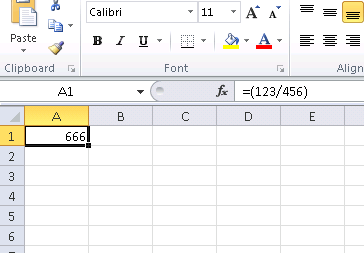
\includegraphics[scale=\NormalScale]{digging_into_code/Excel_prank.png}
\caption{\RU{Пранк сработал}\EN{The practical joke worked}}
\end{figure}

\RU{Если попробовать ту же версию Excel, только x64, то окажется что там инструкций \FDIV всего 12, 
причем нужная нам\EMDASH{}третья по счету.}
\EN{If we try the same Excel version, but in x64,
we will find only 12 \FDIV instructions there,
and the one we looking for is the third one.}

\begin{lstlisting}
tracer.exe -l:excel.exe bpx=excel.exe!BASE+0x1B7FCC,set(st0,666)
\end{lstlisting}

\myindex{x86!\Instructions!DIVSD}
\RU{Видимо, все дело в том, что много операций деления переменных типов \Tfloat и \Tdouble 
компилятор заменил на SSE-инструкции вроде \TT{DIVSD}, 
коих здесь теперь действительно много (\TT{DIVSD} присутствует в количестве 268 инструкций).}
\EN{It seems that a lot of division operations of \Tfloat and \Tdouble types, were replaced by the compiler with SSE instructions
like \TT{DIVSD} (\TT{DIVSD} is present 268 times in total).}

\chapter{\IFRU{Подозрительные паттерны кода}{Suspicious code patterns}}

\section{\IFRU{Инструкции XOR}{XOR instructions}}
\index{x86!\Instructions!XOR}

\IFRU{Инструкции вроде}{instructions like} \TT{XOR op, op} (\IFRU{например}{for example}, \TT{XOR EAX, EAX}) 
\IFRU{обычно используются для обнуления регистра,
однако, если операнды разные, то применяется операция именно}{are usually used for setting register value
to zero, but if operands are different,} \IT{\IFRU{исключающего или}{exclusive or}}\EN{ operation
is executed}.
\IFRU{Эта операция очень редко применяется в обычном программировании, но применяется очень часто в криптографии,
включая любительскую}{This operation is rare in common programming, but used often in cryptography,
including amateur}.
\IFRU{Особенно подозрительно, если второй операнд это большое число}{Especially suspicious case if the
second operand is big number}.
\IFRU{Это может указывать на шифрование, вычисление контрольной суммы, итд}
{This may points to encrypting/decrypting, checksum computing, etc}.\\
\\
\IFRU{Одно из исключений из этого наблюдения о котором стоит сказать, то, что генерация и проверка значения ``канарейки''
(\ref{subsec:BO_protection}) часто происходит используя инструкцию \XOR}
{One exception to this observation worth to note is ``canary'' (\ref{subsec:BO_protection}) generation and checking is often done using \XOR
instruction}. \\
\\
\index{AWK}
\IFRU{Этот AWK-скрипт можно использовать для обработки листингов (.lst) созданных \IDA{}}
{This AWK script can be used for processing \IDA{} listing (.lst) files}:

\begin{lstlisting}
gawk -e '$2=="xor" { tmp=substr($3, 0, length($3)-1); if (tmp!=$4) if($4!="esp") if ($4!="ebp") { print $1, $2, tmp, ",", $4 } }' filename.lst
\end{lstlisting}

\IFRU{Нельзя также забывать,
что если использовать подобный скрипт, то, возможно, он захватит и неверно дизассемблированный
код}{It is also worth to note that such script may also capture incorrectly disassembled code} 
(\ref{sec:incorrectly_disasmed_code}).

\section{\IFRU{Вручную написанный код на ассемблере}{Hand-written assembly code}}

\index{Function prologue}
\index{Function epilogue}
\index{x86!\Instructions!LOOP}
\index{x86!\Instructions!RCL}
\IFRU{Современные компиляторы не генерируют инструкции \TT{LOOP} и \TT{RCL}. 
С другой стороны, эти инструкции хорошо знакомы кодерам, предпочитающим писать прямо на ассемблере. 
Подобные инструкции отмечены как (M) в списке инструкций в приложении: \ref{sec:x86_instructions}.
Если такие инструкции встретились, можно сказать с какой-то вероятностью, что этот фрагмент кода написан вручную.}
{Modern compilers do not emit \TT{LOOP} and \TT{RCL} instructions.
On the other hand, these instructions are well-known to coders who like to code in straight assembly language.
If you spot these, it can be said, with a high probability, this fragment of code is hand-written.
Such instructions are marked as (M) in the instructions list in appendix: \ref{sec:x86_instructions}.}\\
\\
\IFRU{Также, пролог/эпилог функции обычно не встречается в ассемблерном коде, написанном вручную.}
{Also function prologue/epilogue is not commonly present in hand-written assembly copy.}\\
\\
\IFRU{Как правило, в вручную написанном коде, нет никакого четкого метода передачи аргументов в 
функцию}
{Commonly there is no fixed system in passing arguments into functions in the hand-written
code}.\\
\\
\IFRU{Пример из ядра}{Example from} Windows 2003\EN{ kernel} 
(\RU{файл }ntoskrnl.exe\EN{ file}):

\begin{lstlisting}
MultiplyTest proc near               ; CODE XREF: Get386Stepping
             xor     cx, cx
loc_620555:                          ; CODE XREF: MultiplyTest+E
             push    cx
             call    Multiply
             pop     cx
             jb      short locret_620563
             loop    loc_620555
             clc
locret_620563:                       ; CODE XREF: MultiplyTest+C
             retn
MultiplyTest endp

Multiply     proc near               ; CODE XREF: MultiplyTest+5
             mov     ecx, 81h
             mov     eax, 417A000h
             mul     ecx
             cmp     edx, 2
             stc
             jnz     short locret_62057F
             cmp     eax, 0FE7A000h
             stc
             jnz     short locret_62057F
             clc
locret_62057F:                       ; CODE XREF: Multiply+10
                                     ; Multiply+18
             retn
Multiply     endp
\end{lstlisting}

\IFRU{Действительно, если заглянуть в исходные коды}{Indeed, if we look into} 
\ac{WRK} v1.2\IFRU{, данный код можно найти в файле}{ source code, this code
can be found easily in the file} 
\IT{WRK-v1.2\textbackslash{}base\textbackslash{}ntos\textbackslash{}ke\textbackslash{}i386\textbackslash{}cpu.asm}.

\section{\IFRU{Использование magic numbers для трассировки}{Using magic numbers while tracing}}

\IFRU{Нередко бывает нужно узнать, как используется то или иное значение прочитанное из файла либо взятое из пакета
принятого по сети. Часто, ручное слежение за нужной переменной это трудный процесс. Один из простых методов (хотя и не
полностью надежный на 100\%) это использование вашей собственной \IT{magic number}.}
{Often, main goal is to get to know, how a value was read from file, or received via network, being used. 
Often, manual tracing of a value is very labouring task. One of the simple methods (however, not 100\% reliable) 
is to use your own \IT{magic number}.}

\IFRU{Это чем-то напоминает компьютерную томографию: пациенту перед сканированием вводят в кровь 
рентгеноконтрастный препарат, хорошо отсвечивающий в рентгеновских лучах. Известно как кровь нормального человека
расходится, например, по почкам, и если в этой крови будет препарат, то при томографии будет хорошо видно,
достаточно ли хорошо кровь расходится по почкам и нет ли там камней, например, и прочих образований.}
{This resembling X-ray computed tomography is some sense: radiocontrast agent is often injected into patient's blood,
which is used for improving visibility of internal structures in X-rays. For example, it is well known how blood of healthy man/woman
percolates in kidneys and if agent is in blood, it will be easily seen on tomography, how good and normal blood was percolating,
are there any stones or tumors.}

\IFRU{Мы можем взять 32-битное число вроде \IT{0x0badf00d}, либо чью-то дату рождения вроде \IT{0x11101979} 
и записать это, занимающее 4 байта число, в какое-либо место файла используемого исследуемой нами программой.}
{We can take a 32-bit number like \IT{0x0badf00d}, or someone's birth date like \IT{0x11101979}
and to write this, 4 byte holding number, to some point in file used by the program we investigate.}

\index{\GrepUsage}
\IFRU{Затем, при трассировки этой программы, в том числе, при помощи \tracer в режиме 
\IT{code coverage}, а затем при помощи
\IT{grep} или простого поиска по текстовому файлу с результатами трассировки, мы можем легко увидеть, в каких местах кода использовалось 
это значение, и как.}
{Then, while tracing this program, with \tracer in the \IT{code coverage} mode, and then, with the help of \IT{grep}
or just by searching in the text file (of tracing results), we can easily see, where the value was used and how.}

\IFRU{Пример результата работы \tracer в режиме \IT{cc}, к которому легко применить утилиту \IT{grep}}{Example 
of \IT{grepable} \tracer results in the \IT{cc} mode}:

\begin{lstlisting}
0x150bf66 (_kziaia+0x14), e=       1 [MOV EBX, [EBP+8]] [EBP+8]=0xf59c934 
0x150bf69 (_kziaia+0x17), e=       1 [MOV EDX, [69AEB08h]] [69AEB08h]=0 
0x150bf6f (_kziaia+0x1d), e=       1 [FS: MOV EAX, [2Ch]] 
0x150bf75 (_kziaia+0x23), e=       1 [MOV ECX, [EAX+EDX*4]] [EAX+EDX*4]=0xf1ac360 
0x150bf78 (_kziaia+0x26), e=       1 [MOV [EBP-4], ECX] ECX=0xf1ac360 
\end{lstlisting}

\IFRU{Это справедливо также и для сетевых пакетов.
Важно только чтобы наш \IT{magic number} был как можно более уникален и не присутствовал в самом коде.}
{This can be used for network packets as well.
It is important to be unique for \IT{magic number} and not to be present in the program's code.}

\newcommand{\DOSBOXURL}{\url{http://blog.yurichev.com/node/55}}

\index{DosBox}
\IFRU{Помимо \tracer, такой эмулятор MS-DOS как DosBox, в режиме heavydebug, может писать в отчет информацию обо всех
состояниях регистра на каждом шаге исполнения программы\footnote{См.также мой пост в блоге об этой возможности в 
DosBox: \DOSBOXURL{}}, так что этот метод может пригодиться и я для исследования программ под DOS.}{Aside of 
\tracer, DosBox (MS-DOS emulator) in heavydebug mode,
is able to write information about all register's states for each executed instruction of program to plain text file\footnote{See also my 
blog post about this DosBox feature: \DOSBOXURL{}}, so this method may be useful for DOS programs as well.}



\chapter{\RU{Прочее}\EN{Other things}}

\ac{RTTI}~(\ref{RTTI})-\RU{информация также может быть полезна для идентификации 
Си++-классов}\EN{data may be also useful for C++ classes identification}.

\chapter{\RU{Старые методы, тем не менее, интересные}
\EN{Old-school techniques, nevertheless, interesting to know}}

\subsection{\IFRU{Сравнение ``снимков'' памяти}{Memory ``snapshots'' comparing}}

\IFRU{Метод простого сравнения двух снимков памяти для поиска изменений часто применялся для взлома игр 
на 8-битных компьютерах и взлома файлов с записанными рекордными очками.}
{The method of simple two memory snapshots comparing in order to see changes, was often used to hack
8-bit computer games and hacking ``high score'' files.}

\IFRU{К примеру, если вы имеете загруженную игру на 8-битном компьютере (где самой памяти не очень много, но игра
занимает еще меньше), и вы знаете что сейчас у вас, условно, 100 пуль, вы можете сделать ``снимок'' всей
памяти и сохранить где-то. Затем просто стреляете куда угодно, у вас станет 99 пуль, сделать второй ``снимок'',
и затем сравнить эти два снимка: где-то наверняка должен быть байт, который в начале был 100, а затем стал 99.}
{For example, if you got some loaded game on 8-bit computer (it's not much memory on these, but game is usually
consumes even less memory) and you know that you have now, let's say, 100 bullets, you can do a ``snapshot''
of all memory and save it to some place. Then shoot somewhere, bullet count now 99, do second ``snapshot''
and then compare both: somewhere should be a byte which was 100 in the beginning and now it's 99.}
\IFRU{Если учесть что игры на тех маломощных домашних компьютерах обычно были написанны на ассемблере и подобные
переменные там были глобальные, то можно с уверенностью сказать, какой адрес в памяти всегда отвечает за количество
пуль. Если поискать в дизассемблированном коде игры все обращения по этому адресу, несложно найти код,
отвечающий за уменьшение пуль и записать туда инструкцию \NOP\footnote{``no operation'', холостая инструкция} 
или несколько \NOP-в, так мы получим игру в которой у игрока всегда будет 100 пуль, например.}
{Considering a fact that these 8-bit games were often written in assembler and such variables were global,
it can be said for sure, which address in memory holding bullets count. If to search all references to that
address in disassembled game code, it's not very hard to find a piece of code decrementing bullets count,
write \NOP instruction\footnote{``no operation'', idle operation} there, or couple of \NOP{}-s, 
we'll have a game with 100 (for example) bullets forever.}
\IFRU{А так как игры на тех домашних 8-битных 
компьютерах всегда загружались по одним и тем же адресам, и версий одной игры редко когда было больше одной,
то геймеры-энтузиасты знали, по какому адресу (используя инструкцию языка BASIC \IT{POKE}\footnote{инструкция языка BASIC записывающая байт по определенному адресу}) что записать после загрузки
игры, чтобы хакнуть её. Это привело к появлению списков ``читов'' состоящих из инструкций \IT{POKE}, публикуемых
в журналах посвященным 8-битным играм. См.также:}{Games on these 8-bit computers was usually loaded on the same
address, also, there were no much different versions of each game (usually, just one version all have),
enthusiastic gamers knew, which byte should be written (using BASIC instruction \IT{POKE}\footnote{BASIC language instruction writting byte on specific address}) to which address in
order to hack it. This led to ``cheat'' lists containing of \IT{POKE} instructions published in magazines related to
8-bit games. See also:} \url{http://en.wikipedia.org/wiki/PEEK\_and\_POKE}.

\IFRU{Точно также легко модифицировать файлы с сохраненными рекордами, кто сколько очков набрал, впрочем, это может
сработать не только с 8-битными играми. Нужно заметить, какой у вас сейчас рекорд и где-то сохранить файл
с очками. Затем, когда очков станет другое количество, просто сравнить два файла, можно даже
DOS-утилитой FC\footnote{утилита MS-DOS для сравнения двух файлов побайтово} (файлы рекордов, часто, бинарные).}
{The same story about modifying ``high score'' files, this may work not only with 8-bit games. Let's notice 
your score count and save the file somewhere. When ``high score'' count will be different, just compare two files,
it can be even done with DOS-utility FC\footnote{MS-DOS utility for binary files comparing} (``high score'' files
are often in binary form).}
\IFRU{Где-то будут отличаться несколько байт, и легко будет увидеть, какие именно отвечают за количество очков. 
Впрочем, разработчики игр осведомлены о таких хитростях и могут защититься от этого.}
{There will be some place where couple of bytes will be different and it will be easy to see which ones are
holding score number.
However, game developers are aware of such tricks and may protect against it.}

% FIXME: пример с какой-то простой игрушкой?



\part{\RU{Специфичное для ОС}\EN{OS-specific}}
\chapter{\RU{Способы передачи аргументов при вызове функций}\EN{Arguments passing methods (calling conventions)}}
\label{sec:callingconventions}

\section{cdecl}
\index{cdecl}
\label{cdecl}

\RU{Этот способ передачи аргументов через стек чаще всего используется в языках \CCpp.}
\EN{This is the most popular method for arguments passing to functions in \CCpp languages.}

\RU{Вызывающая функция заталкивает в стек аргументы в обратном порядке: сначала последний аргумент в стек, 
затем предпоследний, и в самом конце ~--- первый аргумент. 
Вызывающая функция должна также затем вернуть \glslink{stack pointer}{указатель стека} в нормальное состояние, 
после возврата вызываемой функции.}
\EN{\Gls{caller} pushing arguments to stack in reverse order: last argument, then penultimate element 
and finally~---first argument.
\Gls{caller} also must return back value of the \gls{stack pointer} (\ESP) to its initial state after \gls{callee} function exit.}

\begin{lstlisting}[caption=cdecl]
push arg3
push arg2
push arg1
call function
add esp, 12 ; returns ESP
\end{lstlisting}

\section{stdcall}
\label{sec:stdcall}
\index{stdcall}

\newcommand{\SIZEOFINT}{\RU{Размер переменной типа \Tint ~--- 4 в x86-системах и 8 в x64-системах}
\EN{Size of \Tint type variable is 4 in x86 systems and 8 in x64 systems}}

\RU{Это почти то же что и \IT{cdecl}, за исключением того, что вызываемая функция сама возвращает \ESP 
в нормальное состояние, выполнив инструкцию \TT{RET x} вместо \RET, где 
\TT{x = количество\_аргументов * sizeof(int)\footnote{\SIZEOFINT}}.
Вызывающая функция не будет корректировать \glslink{stack pointer}{указатель стека} при помощи инструкции \TT{add esp, x}.}
\EN{Almost the same thing as \IT{cdecl}, with the exception the \gls{callee} set \ESP to initial state executing \TT{RET x} instruction instead of \RET, where
\TT{x = arguments number * sizeof(int)\footnote{\SIZEOFINT}}.
\Gls{caller} will not adjust \gls{stack pointer} by \TT{add esp, x} instruction.}

\begin{lstlisting}[caption=stdcall]
push arg3
push arg2
push arg1
call function

function:
... do something ...
ret 12
\end{lstlisting}

\RU{Этот способ используется почти везде в системных библиотеках win32, 
но не в win64 (о win64 смотрите ниже).}
\EN{The method is ubiquitous in win32 standard libraries, but not in win64 (see below about win64).} \\
\\
\RU{Например, мы можем взять ф-цию из}\EN{For example, we may take the function from} 
\ref{src:passing_arguments_ex} \RU{и изменить её немного добавив модификатор}\EN{and change it
slightly by adding} \TT{\_\_stdcall}\EN{ modifier}:

\begin{lstlisting}
int __stdcall f2 (int a, int b, int c)
{
	return a*b+c;
};
\end{lstlisting}

\RU{Он будет скомпилирован почти так же как и}\EN{It will be compiled in almost the same way as} 
\ref{src:passing_arguments_ex_MSVC_cdecl},
\RU{но вы увидите}\EN{but you will see} \TT{RET 12} \RU{вместо}\EN{instead of} \TT{RET}. 
\ac{SP} \RU{не будет корректироваться в \glslink{caller}{вызывающей ф-ции}}
\EN{is not aligned in \gls{caller}}.

\RU{Как следствие, количество аргументов ф-ции легко узнать из инструкции}\EN{As a consequence, 
number of function arguments can be easily deduced from} \TT{RETN n} \RU{просто разделите
$n$ на 4}\EN{instruction: just divide $n$ by 4}.

\lstinputlisting[caption=MSVC 2010]{OS/calling_conventions/stdcall_ex.asm}

\subsection{\RU{Функции с переменным количеством аргументов}\EN{Variable arguments number functions}}

\RU{Функции вроде \printf, должно быть, единственный случай функций в \CCpp с переменным количеством аргументов,
но с их помощью можно легко проследить очень важную разницу между \IT{cdecl} и \IT{stdcall}.
Начнем с того, что компилятор знает сколько аргументов было у \printf.}
\EN{\printf-like functions are, probably, the only case of variable arguments functions in \CCpp,
but it is easy to illustrate an important difference between \IT{cdecl} and \IT{stdcall} with the help of it.
Let's start with the idea the compiler knows argument count of each \printf function calling.}
\RU{Однако, вызываемая функция \printf, которая уже давно скомпилирована 
и находится в системной библиотеке MSVCRT.DLL (если говорить о Windows), 
не знает сколько аргументов ей передали, хотя может установить их количество по строке формата.}
\EN{However, called \printf, which is already compiled and located in MSVCRT.DLL (if to talk about Windows),
has not any information about how much arguments were passed, however it can determine it from format string.}
\RU{Таким образом, если бы \printf была \IT{stdcall}-функцией и возвращала
\glslink{stack pointer}{указатель стека}
в первоначальное состояние 
подсчитав количество аргументов в строке формата, это была бы потенциально опасная ситуация, 
когда одна опечатка программиста могла бы вызывать неожиданные падения программы. 
Таким образом, для таких функций \IT{stdcall} явно не подходит, а подходит \IT{cdecl}.}
\EN{Thus, if \printf would be \IT{stdcall}-function and restored \gls{stack pointer} to its initial state by counting
number of arguments in format string, this could be dangerous situation, when one programmer's typo may
provoke sudden program crash.
Thus it is not suitable for such functions to use \IT{stdcall}, \IT{cdecl} is better.}

\section{fastcall}
\label{fastcall}
\index{fastcall}

\RU{Это общее название для передачи некоторых аргументов через регистры, а всех остальных ~--- через стек.На более старых процессорах, это работало потенциально быстрее чем \IT{cdecl}/\IT{stdcall} (ведь стек
в памяти использовался меньше).
Впрочем, на современных, намного более сложных CPU, выигрыша может не быть.}
\EN{That's general naming for a method of passing some of arguments via registers and all 
other~---via stack. It worked faster than \IT{cdecl}/\IT{stdcall} on older CPUs 
(because of smaller stack pressure).
It will not help to gain performance on modern much complex CPUs, however.}

\RU{Это не стандартизированный способ, поэтому разные компиляторы делают это по-своему. 
Разумеется, если у вас есть, скажем, две DLL, одна использует другую, и обе они собраны с \IT{fastcall}
но разными компиляторами, очень вероятно, будут проблемы.}
\EN{it is not a standardized way, so, various compilers may do it differently.
Well known caveat: if you have two DLLs, one uses another, and they are built by different compilers with 
different \IT{fastcall} calling conventions.}

\RU{MSVC и GCC передает первый и второй аргумент через \ECX и \EDX а остальные аргументы через стек.}
\EN{Both MSVC and GCC passing first and second argument via \ECX and \EDX and other arguments via stack.}

\RU{\glslink{stack pointer}{Указатель стека} должен быть возвращен в первоначальное состояние вызываемой функцией, 
как в случае \IT{stdcall}.}
\EN{\Gls{stack pointer} must be restored to initial state by \gls{callee} (like in \IT{stdcall}).}

\begin{lstlisting}[caption=fastcall]
push arg3
mov edx, arg2
mov ecx, arg1
call function

function:
.. do something ..
ret 4
\end{lstlisting}

\RU{Например, мы можем взять ф-цию из}\EN{For example, we may take the function from} 
\ref{src:passing_arguments_ex} \RU{и изменить её немного добавив модификатор}\EN{and change it
slightly by adding} \TT{\_\_fastcall}\EN{ modifier}:

\begin{lstlisting}
int __fastcall f3 (int a, int b, int c)
{
	return a*b+c;
};
\end{lstlisting}

\RU{Вот как он будет скомпилирован}\EN{Here is how it will be compiled}:

\lstinputlisting[caption=MSVC 2010 /Ox /Ob0]{OS/calling_conventions/fastcall_ex.asm}

\RU{Видно что \glslink{callee}{вызываемая ф-ция} сама возвращает}
\EN{We see that a \gls{callee} returns} \ac{SP} 
\RU{при помощи инструкции}\EN{by} \TT{RETN} \RU{с операндом}\EN{instruction with operand}.
\RU{Так что и здесь можно легко вычислять количество аргументов}\EN{Which means, number of arguments
can be deduced easily here as well}.

\subsection{GCC regparm}

\newcommand{\URLREGPARMM}{\url{http://www.ohse.de/uwe/articles/gcc-attributes.html\#func-regparm}}

\RU{Это в некотором роде, развитие \IT{fastcall}\footnote{\URLREGPARMM}. 
Опцией \TT{-mregparm=x} можно указывать, 
сколько аргументов компилятор будет передавать через регистры. Максимально 3. 
В этом случае будут задействованы регистры \EAX, \EDX и \ECX.}
\EN{It is \IT{fastcall} evolution\footnote{\URLREGPARMM} is some sense.
With the \TT{-mregparm} option it is possible to set, how many arguments will be passed via registers. 
3 at maximum.
Thus, \EAX, \EDX and \ECX registers are to be used.}

\RU{Разумеется, если аргументов у функции меньше трех, то будет задействована только часть регистров.}
\EN{Of course, if number of arguments is less then 3, not all 3 registers are to be used.}

\RU{Вызывающая функция возвращает \glslink{stack pointer}{указатель стека} в первоначальное состояние.}
\EN{\Gls{caller} restores \gls{stack pointer} to its initial state.}

\RU{Для примера, см.}\EN{For the example, see} (\ref{regparm}).

\subsection{Watcom/OpenWatcom}
\index{OpenWatcom}

\RU{Здесь это называется}\EN{It is called} ``register calling convention''\EN{ here}.
\RU{Первые 4 аргумента передаются через регистры}\EN{First 4 arguments are passed via}
\EAX, \EDX, \EBX \AndENRU \ECX\EN{ registers}.
\RU{Все остальные}\EN{All the rest}\EMDASH{}\RU{через стек}\EN{via stack}.
\RU{Функции имеют символ подчеркивания добавленный к концу имени ф-ции, для отличия их от тех,
которые имеют другой способ передачи аргументов}
\EN{Functions have underscore added to the function name in order to distinguish them from 
those having other calling convention}.

\section{thiscall}
\index{thiscall}

\RU{В С++, это передача в функцию-метод указателя \ITthis на объект.}
\EN{In C++, it is a \ITthis pointer to object passing into function-method.}

\RU{В MSVC указатель \ITthis обычно передается в регистре \ECX.}
\EN{In MSVC, \ITthis is usually passed in the \ECX register.}

\RU{В GCC указатель \ITthis обычно передается как самый первый аргумент. 
Таким образом, внутри будет видно: у всех функций-методов на один аргумент больше.}
\EN{In GCC, \ITthis pointer is passed as a first function-method argument.
Thus it will be seen: internally, all function-methods has extra argument.}

\RU{Для примера, см.}\EN{For the example, see} (\ref{thiscall}).

\section{x86-64}
\index{x86-64}

\subsection{Windows x64}
\label{sec:callingconventions_win64}

\RU{В win64 метод передачи всех параметров немного похож на \TT{fastcall}. 
Первые 4 аргумента записываются в регистры \RCX, \RDX, \Reg{8}, \Reg{9}, а остальные ~--- в стек. 
Вызывающая функция также должна подготовить место из 32 байт или для четырех 64-битных значений, 
чтобы вызываемая функция могла сохранить там первые 4 аргумента. 
Короткие функции могут использовать переменные прямо из регистров, 
но б\'{о}льшие могут сохранять их значения на будущее.}
\EN{The method of arguments passing in Win64 is somewhat resembling to \TT{fastcall}.
First 4 arguments are passed via \RCX, \RDX, \Reg{8}, \Reg{9}, other~---via stack.
\Gls{caller} also must prepare a space for 32 bytes or 4 64-bit values,
so then \gls{callee} can save there first 4 arguments.
Short functions may use argument values just from registers,
but larger may save its values for further use.}

\RU{Вызывающая функция должна вернуть \glslink{stack pointer}{указатель стека} 
в первоначальное состояние}
\EN{\Gls{caller} also must return \gls{stack pointer} into initial state}.

\RU{Это же соглашение используется и в системных библиотеках Windows x86-64 
(вместо \IT{stdcall} в win32).}
\EN{This calling convention is also used in Windows x86-64 system DLLs 
(instead of \IT{stdcall} in win32).}

\RU{Пример}\EN{Example}:

\lstinputlisting{OS/calling_conventions/x64.c}

\lstinputlisting[caption=MSVC 2012 /0b]{OS/calling_conventions/x64_MSVC_Ob.asm}

\index{Scratch space}
\RU{Здесь мы легко видим как 7 аргументов передаются: 4 через регистры и остальные 3 через стек}
\EN{Here we clearly see how 7 arguments are passed: 4 via registers and the rest 3 via stack}.
\RU{Код пролога ф-ции f1() сохраняет аргументы в ``scratch space'' --- место в стеке предназначенное
именно для этого}
\EN{The code of f1() function's prologue saves the arguments in ``scratch space''---a space in the stack
intended exactly for the purpose}.
\RU{Это делается потому что компилятор может быть не уверен, достаточно ли ему будет остальных регистров
для работы исключая эти 4, которые иначе будут заняты аргументами до конца исполнения ф-ции}
\EN{It is done because compiler may not be sure if it will be enough to use other registers without these 4,
which will otherwise be occupied by arguments until function execution end}.
\RU{Выделение ``scratch space'' в стеке лежит на ответственности вызывающей ф-ции}
\EN{The ``scratch space'' allocation in the stack is on the caller's shoulders}.

\lstinputlisting[caption=MSVC 2012 /Ox /0b]{OS/calling_conventions/x64_MSVC_Ox_Ob.asm}

\RU{Если компилировать этот пример с оптимизацией, то выйдет почти то же самое, только ``scratch space''
не используется, потому что незачем}
\EN{If to compile the example with optimization switch, it is almost the same, but ``scratch space''
is not used, because no need to}.

\RU{Обратите также внимание на то как MSVC 2012 оптимизирует примитивную загрузку значений в регистры
используя \LEA (\ref{sec:LEA})}
\EN{Also take a look on how MSVC 2012 optimizes primitive value loads into registers by using 
\LEA (\ref{sec:LEA})}.
\RU{Я не уверен, что это того стоит, но может быть}\EN{I'm not sure if it worth so, but maybe}.

\subsubsection{\RU{Передача \ITthis}\EN{\ITthis passing}}

\RU{Указатель }\ITthis \RU{передается через}\EN{pointer is passed in} \RCX, 
\RU{первый аргумент метода через}\EN{first method argument in} \RDX, \RU{итд}\EN{etc}.
\RU{Для примера, см. также}\EN{See also for an example}: \ref{simple_CPP_MSVC_x64}.
 
\subsection{Linux x64}

\RU{Метод передачи аргументов в Linux для x86-64 почти такой же, как и в Windows, но 6 регистров
используется вместо 4 (\RDI, \RSI, \RDX, \RCX, \Reg{8}, \Reg{9}), и здесь нет ``scratch space'', 
но \gls{callee}
может сохранять значения регистров в стеке, если нужно}
\EN{The way arguments passed in Linux for x86-64 is almost the same as in Windows, but 6 registers are
used instead of 4 (\RDI, \RSI, \RDX, \RCX, \Reg{8}, \Reg{9}) and there are no ``scratch space'', 
but \gls{callee}
may save register values in the stack, if it needs to}.

\lstinputlisting[caption=GCC 4.7.3 -O3]{OS/calling_conventions/x64_linux_O3.s}

\RU{N.B.: здесь значения записываются в 32-битные части регистров (например EAX) а не в весь 64-битный
регистр (RAX).
Это связано с тем что в x86-64,
запись в младшую 32-битную часть 64-битного регистра автоматически обнуляет старшие 32 бита.
Вероятно, это сделано для упрощения портирования кода под x86-64.}
\EN{N.B.: here values are written into 32-bit parts of registers (e.g., EAX) but not to the whole 64-bit 
register (RAX).
This is because each write to low 32-bit part of register automatically clears high 32 bits.
Supposedly, it was done for x86-64 code porting simplification.}

\section{\RU{Возвращение переменных типа \Tfloat, \Tdouble}\EN{Returning values of \Tfloat and \Tdouble type}}
\index{float}
\index{double}

\RU{Во всех соглашениях кроме Win64, переменная типа \Tfloat или \Tdouble возвращается через регистр FPU \ST{0}.}
\EN{In all conventions except of Win64, values of type \Tfloat or \Tdouble are returning via the FPU register \ST{0}.}

\RU{В Win64 переменные типа \Tfloat и \Tdouble возвращаются в регистре \XMM{0} вместо \ST{0}.}
\EN{In Win64, values of \Tfloat and \Tdouble types are returned in the \XMM{0} register instead of the \ST{0}.}

\section{\RU{Модификация аргументов}\EN{Modifying arguments}}

\RU{Иногда программисты на \CCpp{} (и не только этих \ac{PL}) задаются вопросом,
что будет если модифицировать аргументы?}
\EN{Sometimes, \CCpp{} programmers (not limited to these \ac{PL}, though),
may ask, what will happen if to modify arguments?}
\RU{Ответ прост: аргументы хранятся в стеке, именно там и будет происходит модификация.}
\EN{The answer is simple: arguments are stored in the stack, that is where modification will occurr.}
\RU{А вызывающие ф-ции не использует их после вызова ф-ции (обратного случая в своей практике я не видел
ни разу).}
\EN{Calling functions are not use them after \gls{callee} exit (I have not seen any opposite case in my practice).}

\lstinputlisting{OS/calling_conventions/change_arguments.c}

\lstinputlisting[caption=MSVC 2012]{OS/calling_conventions/change_arguments.asm}

\RU{Следовательно, модифицировать аргументы ф-ции можно запросто.}\EN{So yes, one may modify arguments easily.}
\RU{Разумеется, если это не}\EN{Of course, if it is not} \IT{references} \InENRU \Cpp{} (\ref{cpp_references}),
\RU{и если вы не модифицируете данные по указателю}\EN{and if you not modify data a pointer pointing to} 
(\RU{тогда эффект распространится не только на текущую ф-цию}
\EN{then the effect will be propagated outside of current function}).


\chapter{Thread Local Storage}
\label{TLS}
\index{TLS}

\RU{Это область данных, отдельная для каждого треда. Каждый тред может хранить там то, что ему нужно}
\EN{It is a data area, specific to each thread. Every thread can store there what it needs}.
\RU{Один из известных примеров, это стандартная глобальная переменная в Си}\EN{One famous example
is C standard global variable} \IT{errno}. 
\RU{Несколько тредов одновременно могут вызывать функции
возвращающие код ошибки в \IT{errno}, поэтому глобальная переменная здесь не будет работать корректно, 
для мультитредовых программ \IT{errno} нужно хранить в в \ac{TLS}.}
\EN{Multiple threads may simultaneously call a functions
which returns error code in the \IT{errno}, so global variable will not work correctly here, for multi-thread programs,
\IT{errno} must be stored in the \ac{TLS}.} \\
\\
\index{\Cpp!C++11}
\RU{В}\EN{In the} C++11 \RU{ввели модификатор}\EN{standard, a new} \IT{thread\_local} 
\RU{, показывающий что каждый тред будет иметь свою версию этой переменной}
\EN{modifier was added, showing that each thread will have its own version of the variable},
\RU{и её можно инициализировать, и она расположена в}\EN{it can be initialized, and it is located in the} \ac{TLS}
\footnote{
\index{C11}
\RU{В C11 также есть поддержка тредов, хотя и опциональная}
\EN{C11 also has thread support, optional though}}:

\begin{lstlisting}[caption=C++11]
#include <iostream>
#include <thread>

thread_local int tmp=3;

int main()
{
	std::cout << tmp << std::endl;
};
\end{lstlisting}
\footnote{\RU{Компилируется в}\EN{Compiled in} MinGW GCC 4.8.1, \RU{но не в}\EN{but not in} MSVC 2012}

\RU{Если говорить о PE-файлах, то в исполняемом файле значение}
\EN{If to say about PE-files, in the resulting executable file, the} \IT{tmp} 
\RU{будет именно в секции отведенной}\EN{variable will be stored in the section devoted to}
\ac{TLS}.

\chapter{\RU{Системные вызовы (syscall-ы)}\EN{System calls (syscall-s)}}

\label{syscalls}
\index{syscall}

\index{kernel space}
\index{user space}
\RU{Как известно, все работающие процессы в \ac{OS} делятся на две категории}\EN{As we know, all running processes
inside \ac{OS} are divided into two categories}:
\RU{имеющие полный доступ ко всему ``железу''}\EN{those having all access to the hardware} (``kernel space'') 
\RU{и не имеющие}\EN{and those have not} (``user space'').

\RU{В первой категории ядро \ac{OS} и, обычно, драйвера}
\EN{There are \ac{OS} kernel and usually drivers in the first category}.

\RU{Во второй категории всё прикладное ПО}\EN{All applications are usually in the second category}.

\RU{Это разделение очень важно для безопасности \ac{OS}:
очень важно чтобы никакой процесс не мог испортить что-то в других процессах
или даже в самом ядре \ac{OS}}
\EN{This separation is crucial for \ac{OS} safety: it is very important not to give to any process possibility to screw up
something in other processes or even in \ac{OS} kernel}.
\index{kernel panic}
\index{BSoD}
\RU{С другой стороны, падающий драйвер или ошибка внутри ядра \ac{OS} обычно приводит к}
\EN{On the other hand, failing driver or error inside \ac{OS} kernel usually lead to} kernel panic \OrENRU \ac{BSOD}.

\RU{Защита x86-процессора устроена так что возможно разделить всё на 4 слоя защиты (rings), но и в Linux,
и в Windows, используются только 2}
\EN{x86-processor protection allows to separate everything into 4 levels of protection (rings), but both in Linux
and in Windows only two are used}: ring0 (``kernel space'') \AndENRU ring3 (``user space'').

\RU{Системные вызовы}\EN{System calls} (syscall-\RU{ы}\EN{s})
\RU{это точка где соединяются вместе оба эти пространства}\EN{is a point where these two areas are connected}.
\RU{Это, можно сказать, самое главное \ac{API} предоставляемое прикладному ПО.}
\EN{It can be said, this is the most principal \ac{API} provided to application software.}

\RU{В \gls{Windows NT} таблица сисколлов находится в \ac{SSDT}}
\EN{As in \gls{Windows NT}, syscalls table reside in \ac{SSDT}}.

\index{Shellcode}
\RU{Работа через syscall-ы популярна у авторов шеллкодов и вирусов,
потому что там обычно бывает трудно определить адреса нужных ф-ций в системных библиотеках,
а syscall-ами проще пользоваться, хотя и придется писать больше
кода из-за более низкого уровня абстракции этого \ac{API}}
\EN{Usage of syscalls is very popular among shellcode and computer viruses authors, 
because it is hard to determine the addresses of
needed functions in the system libraries, while it is easier to use syscalls, however, much more code should be
written due to lower level of abstraction of the \ac{API}}.
\RU{Также нельзя еще забывать, что номера syscall-ов могут отличаться от версии к версии OS.}
\EN{It is also worth noting that the syscall numbers may be different in various OS versions.}

\section{Linux}

\index{x86!\Instructions!INT!INT 0x80}
\RU{В Linux вызов syscall-а обычно происходит через}\EN{In Linux, syscall is usually called via} \TT{int 0x80}.
\RU{В регистре}\EN{Call number is passed in the} \EAX \RU{передается номер вызова,
в остальных регистрах ~---- параметры}\EN{register, and any other parameters~---in the other registers}.

\lstinputlisting[caption=\RU{Простой пример использования пары syscall-ов}\EN{Simple example of two syscalls usage}]
{OS/linux_syscall.s}

\RU{Компиляция}\EN{Compilation}:

\begin{lstlisting}
nasm -f elf32 1.s
ld 1.o
\end{lstlisting}

\RU{Полный список syscall-ов в}\EN{The full list of syscalls in} Linux: \url{http://go.yurichev.com/17319}.

\RU{Для перехвата и трассировки системных вызовов в Linux, можно применять}
\EN{For system calls intercepting and tracing in Linux,} strace(\myref{strace})\EN{ can be used}.

\section{Windows}

\index{x86!\Instructions!INT!INT 0x2e}
\index{x86!\Instructions!SYSENTER}

\RU{Вызов происходит через}\EN{They are called by} \TT{int 0x2e} 
\RU{либо используя специальную x86-инструкцию}\EN{or using special x86 instruction} \TT{SYSENTER}.

\RU{Полный список syscall-ов в}\EN{The full list of syscalls in} Windows: \url{http://go.yurichev.com/17320}.

\RU{Смотрите также}\EN{Further reading}:

``Windows Syscall Shellcode'' by Piotr Bania:\\
\url{http://go.yurichev.com/17321}.



\chapter{Linux}
\section{\CapitalPICcode}
\index{\PICcode}
\index{Linux}
\label{sec:PIC}

\RU{Во время анализа динамических библиотек (.so) в Linux, часто можно заметить такой шаблонный код}\EN{While analyzing Linux shared (.so) libraries, one may frequently spot this code pattern}:

\begin{lstlisting}[caption=libc-2.17.so x86]
.text:0012D5E3 __x86_get_pc_thunk_bx proc near         ; CODE XREF: sub_17350+3
.text:0012D5E3                                         ; sub_173CC+4 ...
.text:0012D5E3                 mov     ebx, [esp+0]
.text:0012D5E6                 retn
.text:0012D5E6 __x86_get_pc_thunk_bx endp

...

.text:000576C0 sub_576C0       proc near               ; CODE XREF: tmpfile+73

...

.text:000576C0                 push    ebp
.text:000576C1                 mov     ecx, large gs:0
.text:000576C8                 push    edi
.text:000576C9                 push    esi
.text:000576CA                 push    ebx
.text:000576CB                 call    __x86_get_pc_thunk_bx
.text:000576D0                 add     ebx, 157930h
.text:000576D6                 sub     esp, 9Ch

...

.text:000579F0                 lea     eax, (a__gen_tempname - 1AF000h)[ebx] ; "__gen_tempname"
.text:000579F6                 mov     [esp+0ACh+var_A0], eax
.text:000579FA                 lea     eax, (a__SysdepsPosix - 1AF000h)[ebx] ; "../sysdeps/posix/tempname.c"
.text:00057A00                 mov     [esp+0ACh+var_A8], eax
.text:00057A04                 lea     eax, (aInvalidKindIn_ - 1AF000h)[ebx] ; "! \"invalid KIND in __gen_tempname\""
.text:00057A0A                 mov     [esp+0ACh+var_A4], 14Ah
.text:00057A12                 mov     [esp+0ACh+var_AC], eax
.text:00057A15                 call    __assert_fail
\end{lstlisting}

\RU{Все указатели на строки корректируются при помощи некоторой константы из регистра \EBX, которая вычисляется в начале каждой функции.}
\EN{All pointers to strings are corrected by some constants and the value in \EBX,
which is calculated at the beginning of each function.}
\RU{Это так называемый адресно-независимый код (\ac{PIC}), он предназначен для исполнения будучи расположенным по любому адресу в памяти, вот почему он не содержит никаких абсолютных адресов в памяти}
\EN{This is the so-called \ac{PIC}, it is intended to be executable if placed at any random point of memory, that is why it cannot contain any absolute memory addresses}.

\RU{\ac{PIC} был очень важен в ранних компьютерных системах и важен сейчас во встраиваемых\footnote{embedded}, не имеющих поддержки виртуальной памяти (все процессы расположены в одном непрерывном блоке памяти)}
\EN{\ac{PIC} was 
crucial in early computer systems and is crucial now in embedded systems without 
virtual memory support (where all processes are placed in a single continuous memory block)}.
\RU{Он до сих пор используется в *NIX системах для динамических библиотек, потому что динамическая библиотека может использоваться одновременно в нескольких процессах, будучи загружена в память только один раз}
\EN{It is also still used in *NIX systems for shared libraries, since they 
are shared across many processes while loaded in memory only once}.
\RU{Но все эти процессы могут загрузить одну и ту же динамическую библиотеку по разным адресам, вот почему динамическая библиотека должна работать корректно, не привязываясь к абсолютным адресам}\EN{But all these processes can 
map the same shared library at different addresses, so that is why
a shared library has to work correctly without using any absolute addresses}.

\RU{Простой эксперимент}\EN{Let's do a simple experiment}:

\begin{lstlisting}
#include <stdio.h>

int global_variable=123;

int f1(int var)
{
    int rt=global_variable+var;
    printf ("returning %d\n", rt);
    return rt;
};
\end{lstlisting}

\RU{Скомпилируем в GCC 4.7.3 и посмотрим итоговый файл .so в}\EN{Let's compile it in GCC 4.7.3 and see the resulting .so file in} \IDA:

\begin{lstlisting}
gcc -fPIC -shared -O3 -o 1.so 1.c
\end{lstlisting}

\begin{lstlisting}[caption=GCC 4.7.3]
.text:00000440                 public __x86_get_pc_thunk_bx
.text:00000440 __x86_get_pc_thunk_bx proc near         ; CODE XREF: _init_proc+4
.text:00000440                                         ; deregister_tm_clones+4 ...
.text:00000440                 mov     ebx, [esp+0]
.text:00000443                 retn
.text:00000443 __x86_get_pc_thunk_bx endp

.text:00000570                 public f1
.text:00000570 f1              proc near
.text:00000570
.text:00000570 var_1C          = dword ptr -1Ch
.text:00000570 var_18          = dword ptr -18h
.text:00000570 var_14          = dword ptr -14h
.text:00000570 var_8           = dword ptr -8
.text:00000570 var_4           = dword ptr -4
.text:00000570 arg_0           = dword ptr  4
.text:00000570
.text:00000570                 sub     esp, 1Ch
.text:00000573                 mov     [esp+1Ch+var_8], ebx
.text:00000577                 call    __x86_get_pc_thunk_bx
.text:0000057C                 add     ebx, 1A84h
.text:00000582                 mov     [esp+1Ch+var_4], esi
.text:00000586                 mov     eax, ds:(global_variable_ptr - 2000h)[ebx]
.text:0000058C                 mov     esi, [eax]
.text:0000058E                 lea     eax, (aReturningD - 2000h)[ebx] ; "returning %d\n"
.text:00000594                 add     esi, [esp+1Ch+arg_0]
.text:00000598                 mov     [esp+1Ch+var_18], eax
.text:0000059C                 mov     [esp+1Ch+var_1C], 1
.text:000005A3                 mov     [esp+1Ch+var_14], esi
.text:000005A7                 call    ___printf_chk
.text:000005AC                 mov     eax, esi
.text:000005AE                 mov     ebx, [esp+1Ch+var_8]
.text:000005B2                 mov     esi, [esp+1Ch+var_4]
.text:000005B6                 add     esp, 1Ch
.text:000005B9                 retn
.text:000005B9 f1              endp
\end{lstlisting}

\newcommand{\retstring}{\IT{<<returning \%d\textbackslash{}n>>}}
\newcommand{\globvar}{\IT{global\_variable}}

\RU{Так и есть: указатели на строку \retstring{} и переменную \globvar{} корректируются при каждом исполнении функции}
\EN{That's it: the pointers to \retstring{} and \globvar{} are to be corrected at each function execution.}
\RU{Функция}\EN{The} \TT{\_\_x86\_get\_pc\_thunk\_bx()} \RU{возвращает адрес точки после вызова самой себя (здесь: \TT{0x57C}) в \EBX}\EN{function returns in \EBX the address of the point after a call to itself (\TT{0x57C} here)}.
\RU{Это очень простой способ получить значение указателя на текущую инструкцию (\EIP) в произвольном месте}
\EN{That's a simple way to get the value of the program counter (\EIP) at some point}.
\RU{Константа}\EN{The} \TT{0x1A84} \RU{связана с разницей между началом этой функции и так называемой}\EN{constant is related to the difference between this function's start and the so-called}
\IT{Global Offset Table Procedure Linkage Table} (GOT PLT), \RU{секцией, сразу же за}\EN{the section right after the} \IT{Global Offset Table} (GOT), \RU{где находится указатель на \globvar{}}\EN{where the pointer to \globvar{} is}.
\IDA \RU{показывает смещения уже обработанными, чтобы их было проще понимать, но на самом деле код такой}\EN{shows these offsets in their processed form to make them easier to understand, but in fact the code is}:

\begin{lstlisting}
.text:00000577                 call    __x86_get_pc_thunk_bx
.text:0000057C                 add     ebx, 1A84h
.text:00000582                 mov     [esp+1Ch+var_4], esi
.text:00000586                 mov     eax, [ebx-0Ch]
.text:0000058C                 mov     esi, [eax]
.text:0000058E                 lea     eax, [ebx-1A30h]
\end{lstlisting}

\RU{Так что, \EBX указывает на секцию \TT{GOT PLT} и для вычисления указателя на \globvar{}, которая хранится в \TT{GOT}, нужно вычесть 0xC}\EN{Here \EBX points to the \TT{GOT PLT} section and to calculate a pointer to \globvar{} (which is stored in 
the \TT{GOT}), \TT{0xC} must be subtracted}.
\RU{А чтобы вычислить указатель на \retstring{}, нужно вычесть \TT{0x1A30}}
\EN{To calculate pointer to the \retstring{} string, \TT{0x1A30} must be subtracted}.

\index{x86-64}
\index{x86!\Registers!RIP}
\RU{Кстати, вот зачем в AMD64 появилась поддержка адресации относительно RIP\footnote{указатель инструкций в AMD64}, просто для упрощения PIC-кода}
\EN{By the way, that is the reason why the AMD64 instruction set supports RIP\footnote{program counter in AMD64}-relative addressing ~--- to simplify PIC-code}.

\RU{Скомпилируем тот же код на Си при помощи той же версии GCC, но для x64}\EN{Let's compile the same C code using the same GCC version, but for x64}.

\index{objdump}
\IDA \RU{упростит код на выходе убирая упоминания RIP, так что я буду использовать \IT{objdump} вместо}
\EN{would simplify the resulting code but would suppress the RIP-relative addressing details, so I will use \IT{objdump} instead to see the everything}:

\begin{lstlisting}
0000000000000720 <f1>:
 720:	48 8b 05 b9 08 20 00 	mov    rax,QWORD PTR [rip+0x2008b9]        # 200fe0 <_DYNAMIC+0x1d0>
 727:	53                   	push   rbx
 728:	89 fb                	mov    ebx,edi
 72a:	48 8d 35 20 00 00 00 	lea    rsi,[rip+0x20]        # 751 <_fini+0x9>
 731:	bf 01 00 00 00       	mov    edi,0x1
 736:	03 18                	add    ebx,DWORD PTR [rax]
 738:	31 c0                	xor    eax,eax
 73a:	89 da                	mov    edx,ebx
 73c:	e8 df fe ff ff       	call   620 <__printf_chk@plt>
 741:	89 d8                	mov    eax,ebx
 743:	5b                   	pop    rbx
 744:	c3                   	ret    
\end{lstlisting}

\TT{0x2008b9} \RU{это разница между адресом инструкции по \TT{0x720} и \globvar{}, 
а \TT{0x20} это разница между инструкцией по \TT{0x72A} и строкой \retstring{}}
\EN{is the difference between the address of the instruction at \TT{0x720} and \globvar{}, and 
\TT{0x20} is the difference between the address of the instruction at 
\TT{0x72A} and the \retstring{} string}.

\RU{Как видно, необходимость очень часто пересчитывать адреса делает исполнение немного медленнее 
(хотя это и стало лучше в x64)}
\EN{As you might see, the need to recalculate addresses frequently makes execution slower 
(it is better in x64, though)}.
\RU{Так что если вы заботитесь о скорости исполнения, то, наверное, нужно задуматься о статической
компоновке (static linking)}
\EN{So it is probably better to link statically if you care about performance} \cite{AgnerFogCPP}.

\subsection{Windows}
\index{Windows!Win32}

\RU{Такой механизм не используется в Windows DLL. Если загрузчику в Windows приходится загружать DLL 
в другое место, он ``патчит'' DLL прямо в памяти (на местах \IT{FIXUP}-ов) чтобы скорректировать 
все адреса.}\EN{The PIC mechanism is not used in Windows DLLs. If the Windows loader needs to load DLL 
on another base address, it ``patches'' the DLL in memory (at the \IT{FIXUP} places) in order to correct 
all addresses.}
\RU{Это приводит к тому что загруженную один раз DLL нельзя использовать одновременно в разных 
процессах, желающих расположить её по разным адресам ~--- потому что каждый загруженный в память 
экземпляр DLL \IT{доводится} до того чтобы работать только по этим адресам.}\EN{This means that several 
Windows processes cannot share an once loaded DLL at different addresses in different process' memory 
blocks~---since each instance that's loaded in memory is \IT{fixed} to work only at these addresses..}

\section{\RU{Трюк с }\IT{LD\_PRELOAD}\EN{ hack} \InENRU Linux}

\index{LD\_PRELOAD}
\label{ld_preload}

\RU{Это позволяет загружать свои динамические библиотеки перед другими, даже перед системными,
такими как}
\EN{This allows us to load our own dynamic libraries before others, even before system ones, like} libc.so.6.

\RU{Что в свою очередь, позволяет ``подставлять'' написанные нами ф-ции перед оригинальными из системных библиотек.}
\EN{What, in turn, allows to ``substitute'' our written functions before original ones in system libraries.}
\RU{Например, легко перехватывать все вызовы к}\EN{For example, it is easy to intercept all calls to the} 
time(), read(), write(), \RU{и т.д}\EN{etc}. \\
\\
\index{uptime}
\RU{Попробуем узнать, сможем ли мы обмануть утилиту \IT{uptime}}\EN{Let's see, if we are able to fool
\IT{uptime} utility}.
\RU{Как известно, она сообщает, как долго компьютер работает}\EN{As we know, it tells how long the computer
is working}.
\index{strace}
\RU{При помощи}\EN{With the help of} strace(\ref{strace}), \RU{можно увидеть, что эту информацию утилита получает из файла}
\EN{it is possible to see that this information the utility takes from the} \TT{/proc/uptime}
\EN{ file}:

\begin{lstlisting}
$ strace uptime 
...
open("/proc/uptime", O_RDONLY)          = 3
lseek(3, 0, SEEK_SET)                   = 0
read(3, "416166.86 414629.38\n", 2047)  = 20
...
\end{lstlisting}

\RU{Это не реальный файл на диске, это виртуальный файл,
содержимое которого генерируется на лету в ядре Linux.}
\EN{It is not a real file on disk, it is a virtual one, its contents is generated on fly in Linux kernel.}
\RU{Там просто два числа}\EN{There are just two numbers}:

\begin{lstlisting}
$ cat /proc/uptime
416690.91 415152.03
\end{lstlisting}

\RU{Из wikipedia, можно узнать}\EN{What we can learn from wikipedia}:

\begin{framed}
\begin{quotation}
The first number is the total number of seconds the system has been up.
The second number is how much of that time the machine has spent idle, in seconds.
\end{quotation}
\end{framed}\footnote{\url{https://en.wikipedia.org/wiki/Uptime}}

\index{\CStandardLibrary!open()}
\index{\CStandardLibrary!read()}
\index{\CStandardLibrary!close()}
\RU{Попробуем написать свою динамическую библиотеку, в которой будет}
\EN{Let's try to write our own dynamic library with the} open(), read(), close() 
\RU{с нужной нам функциональностью}\EN{functions working as we need}.

\RU{Во-первых, наш open() будет сравнивать имя открываемого файла с тем что нам нужно, и если да, 
то будет запоминать дескриптор открытого файла.}
\EN{At first, our open() will compare name of file to be opened with what we need and if it is so,
it will write down the descriptor of the file opened.}
\RU{Во-вторых, read(), если будет вызываться для этого дескриптора, будет подменять вывод,
а в остальных случаях, будет вызывать настоящий}
\EN{At second, read(), if it will be called for this file descriptor, will substitute output,
and in other cases, will call original} read() \RU{из}\EN{from} libc.so.6.
\RU{А также}\EN{And also} close(), \RU{будет следить, закрывается ли файл за которым мы следим.}
\EN{will note, if the file we are currently follow is to be closed.}

\index{dlopen()}
\index{dlsym()}
\RU{Для того чтобы найти адреса настоящих ф-ций в libc.so.6, используем dlopen() и dlsym().}
\EN{We will use the dlopen() and dlsym() functions to determine original addresses of functions in libc.so.6.}

\RU{Нам это нужно, потому что нам нужно передавать управление ``настоящим'' ф-циями.}
\EN{We need them because we must pass control to ``real'' functions.}

\index{\CStandardLibrary!strcmp()}
\RU{С другой стороны, если бы мы перехватывали, скажем, strcmp(),
и следили бы за всеми сравнениями строк в программе, 
то, наверное, strcmp() можно было бы и самому реализовать, не
пользуясь настоящей ф-цией}
\EN{On the other hand, if we could intercept e.g. strcmp(), and follow each string
comparisons in program, then strcmp() could be implemented easily on one's own, while not
using original function}
\footnote{\RU{Например, посмотрите как обеспечивается простейший перехват strcmp()}
\EN{For example, here is how simple strcmp() interception is works} \InENRU
\RU{статье}\EN{article}
\footnote{\url{http://yurichev.com/mirrors/LD\_PRELOAD/Yong\%20Huang\%20LD\_PRELOAD.txt}}
\RU{от}\EN{from} Yong Huang}.

\lstinputlisting{OS/LD_PRELOAD/fool_uptime.c}
% FIXME: add URL to github source

\RU{Компилируем как динамическую библиотеку}\EN{Let's compile it as common dynamic library}:

\begin{lstlisting}
gcc -fpic -shared -Wall -o fool_uptime.so fool_uptime.c -ldl
\end{lstlisting}

\RU{Запускаем \IT{uptime}, подгружая нашу библиотеку перед остальными}\EN{Let's run \IT{uptime}
while loading our library before others}:

\begin{lstlisting}
LD_PRELOAD=`pwd`/fool_uptime.so uptime
\end{lstlisting}

\RU{Видим такое}\EN{And we see}:

\begin{lstlisting}
 01:23:02 up 24855 days,  3:14,  3 users,  load average: 0.00, 0.01, 0.05
\end{lstlisting}

\RU{Если переменная окружения}\EN{If the} \IT{LD\_PRELOAD} 
\RU{будет всегда указывать на путь и имя файла нашей библиотеки, то она будет
загружаться для всех запускаемых программ.}
\EN{environment variable will always points to filename and path of our library, it will be loaded
for all starting programs.} \\
\\
\RU{Еще примеры}\EN{More examples}:

\begin{itemize}
\RU{\item
\RU{Перехват}\EN{Intercepting} time() \InENRU Sun Solaris \url{http://yurichev.com/mirrors/LD_PRELOAD/sun_hack.txt}
}

\item
\RU{Очень простой перехват}\EN{Very simple interception of the} strcmp() (Yong Huang) 
\url{http://yurichev.com/mirrors/LD\_PRELOAD/Yong\%20Huang\%20LD\_PRELOAD.txt}

\item
Kevin Pulo --- Fun with LD\_PRELOAD. \RU{Много примеров и идей}\EN{A lot of examples and ideas}.
\url{http://yurichev.com/mirrors/LD_PRELOAD/lca2009.pdf}

\item
\RU{Перехват ф-ций работы с файлами для компрессии и декомпрессии файлов на лету}
\EN{File functions interception for compression/decompression files on fly} (zlibc). \url{ftp://metalab.unc.edu/pub/Linux/libs/compression}

\end{itemize}


\chapter{Windows NT}
\section{CRT (win32)}
\label{sec:CRT}
\index{CRT}

\RU{Начинается ли исполнение программы прямо с ф-ции \main{}}
\EN{Does program execution starts right at the \main{} function}?
\RU{Нет, не начинается}\EN{No, it is not}.
\RU{Если открыть любой исполняемый файл в \IDA или Hiew, то \ac{OEP} указывает на совсем другой код}
\EN{If we would open any executable file in \IDA or HIEW, we will see \ac{OEP} pointing to another code}.
\RU{Это код, который делает некоторые приготовления перед тем как запустить ваш код}
\EN{This is a code doing some maintenance and preparations before passing control flow to our code}.
\RU{Он называется стартап-код или CRT-код (C RunTime)}\EN{It is called startup-code or CRT-code (C RunTime)}. \\
\\
\RU{Ф-ция \main{} принимает на вход массив из параметров, переданных в командной строке, а также
переменные окружения}\EN{\main{} function takes an array of arguments passed in the command line, and also
environment variables}.
\RU{Но в реальности в программу передается командная строка в виде простой строки, это именно
CRT-код находит там пробелы и разрезает строку на части}\EN{But in fact, a generic string is passed to the program,
CRT-code will find spaces in it and cut by parts}.
\RU{CRT-код также готовит массив переменных окружения \TT{envp}}\EN{CRT-code is also prepares environment
variables array \TT{envp}}.
\RU{В \ac{GUI}-приложениях win32, вместо \main{} имеется ф-ция \TT{WinMain} со своими аргументами}
\EN{As of \ac{GUI} win32 applications, \TT{WinMain} is used instead of \main{}, having their own arguments}:

\begin{lstlisting}
int CALLBACK WinMain(
  _In_  HINSTANCE hInstance,
  _In_  HINSTANCE hPrevInstance,
  _In_  LPSTR lpCmdLine,
  _In_  int nCmdShow
);
\end{lstlisting}

\RU{CRT-код готовит и их}\EN{CRT-code prepares them as well}.

\RU{А также, число, возвращаемое ф-цией \main{}, это код ошибки возвращаемый программой}
\EN{Also, the number returned by \main{} function is an exit code}.
\RU{В CRT это значение передается в \TT{ExitProcess()}, принимающей в качестве аргумента код ошибки}
\EN{It may be passed in CRT to the \TT{ExitProcess()} function, taking exit code as argument}. \\
\\
\RU{Как правило, каждый компилятор имеет свой CRT-код}\EN{Usually, each compiler has its own CRT-code}. \\
\\
\RU{Вот типичный для MSVC 2008 CRT-код}\EN{Here is a typical CRT-code for MSVC 2008}.

\lstinputlisting[numbers=left]{OS/win32_CRT/crt_msvc_2008.asm}

\RU{Здесь можно увидеть по крайней мере вызов
ф-ции}\EN{Here we may see calls to} \TT{GetCommandLineA()} (\LineENRU 62), 
\RU{затем}\EN{then to} \TT{setargv()} (\LineENRU 66) \AndENRU \TT{setenvp()} (\LineENRU 74),
\RU{которые, видимо, заполняют глобальные переменные-указатели}\EN{which are, apparently, fills global variables}
\TT{argc}, \TT{argv}, \TT{envp}.

\RU{В итоге, вызывается \main{} с этими аргументами}\EN{Finally, \main{} is called with these arguments} 
(\LineENRU 97).

\RU{Также имеются вызовы ф-ций с говорящими именами вроде}\EN{There are also calls to the functions
having self-describing names like} \TT{heap\_init()} (\LineENRU 35), \TT{ioinit()} (\LineENRU 54).

\RU{\glslink{heap}{Куча} действительно инициализируется в \ac{CRT}}
\EN{\glslink{heap}{Heap} is indeed initialized in \ac{CRT}}.
\RU{Если вы попытаетесь использовать}\EN{If you will try to use} \TT{malloc()} 
\RU{в программе без}\EN{in the program without} CRT,
\RU{программа упадет с такой ошибкой}\EN{the program exiting abnormally with the error}:

\begin{lstlisting}
runtime error R6030
- CRT not initialized
\end{lstlisting}

\RU{Инициализация глобальных объектов в \Cpp происходит до вызова \main{}, именно в \ac{CRT}}
\EN{Global object initializations in \Cpp is also occurred in the \ac{CRT} before \main{} execution}: 
\ref{sec:std_string_as_global_variable}.

\RU{Значение, возвращаемое из}\EN{A value} \main{} \RU{передается или в}\EN{returns is passed to} \TT{cexit()}, 
\RU{или же в}\EN{or to} \TT{\$LN32}, \RU{которая далее вызывает}\EN{which in turn calling} \TT{doexit()}.

\RU{Можно ли обойтись без \ac{CRT}? Можно, если вы знаете что делаете.}\EN{Is it possible to get rid of \ac{CRT}?
Yes, if you know what you do.}

\RU{В линкере от \ac{MSVC} точка входа задается опцией \TT{/ENTRY}}
\EN{\ac{MSVC} linker has \TT{/ENTRY} option for setting entry point}.

\begin{lstlisting}
#include <windows.h>

int main()
{
	MessageBox (NULL, "hello, world", "caption", MB_OK);
};
\end{lstlisting}

\RU{Компилируем в}\EN{Let's compile it in} MSVC 2008.

\begin{lstlisting}
cl no_crt.c user32.lib /link /entry:main
\end{lstlisting}

\RU{Получаем вполне работающий .exe размером 2560 байт, внутри которого есть только PE-заголовок, инструкции, 
вызывающие \TT{MessageBox},
две строки в сегменте данных, импортируемая из \TT{user32.dll} ф-ция \TT{MessageBox}, и более ничего}
\EN{We will get a runnable .exe with size 2560 bytes, there are PE-header inside, instructions calling
\TT{MessageBox}, two strings in the data segment,
\TT{MessageBox} function imported from \TT{user32.dll} and nothing else}.

\RU{Это работает, но вы уже не сможете вместо \main{} написать \TT{WinMain} с его четырьмя аргументами}
\EN{This works, but you will not be able to write \TT{WinMain} with its 4 arguments instead of \main{}}.
\RU{Вернее, написать-то сможете, но доступа к этим аргументам не будет, 
потому что они не будут подготовлены на момент исполнения}\EN{To be correct, you will be able to write so,
but arguments will not be prepared at the moment of execution}.

\RU{Кстати, можно еще короче сделать .exe если уменьшить 
выравнивание \ac{PE}-секций (которое, по умолчанию, 4096 байт)}\EN{By the way, it is possible to make .exe even
shorter by doing \ac{PE}-section aligning less than default 4096 bytes}.

\begin{lstlisting}
cl no_crt.c user32.lib /link /entry:main /align:16
\end{lstlisting}

\RU{Линкер скажет}\EN{Linker will say}:

\begin{lstlisting}
LINK : warning LNK4108: /ALIGN specified without /DRIVER; image may not run
\end{lstlisting}

\RU{Получим .exe размером 720 байт}\EN{We getting .exe of 720 bytes size}.
\RU{Он запускается в}\EN{It running in} Windows 7 x86, \RU{но не}\EN{but not in} x64 
(\RU{там выдает ошибку при загрузке}\EN{the error message will be showed when trying to execute}).
\RU{При желании, размер можно еще сильнее ужать, но, как видно, 
возникают проблемы с совместимостью с разными версиями Windows}\EN{By applying even more efforts, it is possible
to make executable even shorter, but as you can see, compatibility problems may arise quickly}.


\section{Win32 PE}
\label{win32_pe}
\index{Windows!Win32}

\acs{PE} \RU{это формат исполняемых файлов, принятый в Windows}\EN{is an executable file format used in
Windows}.

\RU{Разница между .exe, .dll, и .sys в том, что у .exe и .sys обычно нет экспортов, только импорты}
\EN{The difference between .exe, .dll and .sys is that .exe and .sys usually do not have exports, only imports}.

\index{OEP}
\RU{У \ac{DLL}, как и у всех PE-файлов, есть точка входа (\ac{OEP})
(там располагается функция DllMain()), но обычно эта функция ничего не делает.}
\EN{A \ac{DLL}, just like any other PE-file, has an entry point (\ac{OEP}) (the function DllMain() is located there) 
but this function usually does nothing.}

.sys \RU{это обычно драйвера устройств}\EN{is usually a device driver}.

\RU{Для драйверов, Windows требует, чтобы контрольная сумма в PE-файле была проставлена
и была верной}
\EN{As of drivers, Windows requires the checksum to be present in the PE file and for it to be correct}
\footnote{\RU{Например}\EN{For example}, Hiew(\myref{Hiew}) \RU{умеет её подсчитывать}\EN{can calculate it}}.

\index{Windows!Windows Vista}
\RU{А начиная с}\EN{Starting at} Windows Vista, 
\RU{файлы драйверов должны быть также подписаны при помощи электронной подписи, 
иначе они не будут загружаться.}
\EN{a driver's files must also be signed with a digital signature. It will fail to load otherwise.}

\index{MS-DOS}
\RU{В начале всякого PE-файла есть крохотная DOS-программа,
выводящая на консоль сообщение вроде}\EN{Every PE file begins with tiny DOS program that prints a
message like} \q{This program cannot be run in DOS mode.}\EMDASH{}%
\RU{если запустить эту программу в DOS либо Windows 3.1 (\ac{OS} не знающие о PE-формате), 
выведется это сообщение.}
\EN{if you run this program in DOS or Windows 3.1 (\ac{OS}-es which are not aware of the PE format), 
this message will be printed.}

\subsection{\RU{Терминология}\EN{Terminology}}

\begin{itemize}
\item
\RU{Модуль}\EN{Module}\EMDASH{}\RU{это отдельный файл}\EN{a separate file}, .exe \OrENRU{} .dll.

\item
	\RU{Процесс}\EN{Process}\EMDASH{}\RU{это некая загруженная в память и работающая программа}\EN{a program
loaded into memory and currently running}.
\RU{Как правило состоит из одного .exe-файла и массы .dll-файлов}\EN{Commonly consists of 
one .exe file and bunch of .dll files}.

\item
	\RU{Память процесса}\EN{Process memory}\EMDASH{}\RU{память с которой работает процесс}\EN{the memory a process
works with}.
\RU{У каждого процесса\EMDASH{}своя}\EN{Each process has its own}.
\RU{Там обычно имеются загруженные модули, память стека, \glslink{heap}{кучи},}
\EN{There usually are loaded modules, memory of the stack, \gls{heap}(s),}\etc{}.

\item
\index{VA}
\ac{VA}\EMDASH{}\RU{это адрес, который будет использоваться в самой программе во время исполнения.}
\EN{an address which is to be used in program while runtime.}

\item
\index{\RU{Базовый адрес}\EN{Base address}}
\RU{Базовый адрес (модуля)}\EN{Base address (of module)}\EMDASH{}
\RU{это адрес, по которому модуль должен быть загружен в пространство процесса.}
\EN{the address within the process memory at which the module is to be loaded.}
\EN{\ac{OS} loader may change it, if the base address is already occupied by another module just loaded before.}
\RU{Загрузчик \ac{OS} может его изменить, если этот базовый адрес уже занят другим модулем, загруженным перед ним.}

\item
\index{RVA}
\ac{RVA}\EMDASH{}\RU{это}\EN{the} \ac{VA}-\RU{адрес минус базовый адрес}\EN{address minus the base address}.
\RU{Многие адреса в таблицах PE-файла используют}
\EN{Many addresses in PE-file tables use}
\ac{RVA}-\RU{адреса}\EN{addresses}.

%\item
%Data directory\EMDASH{}...

\item 
\index{Windows!IAT}
\ac{IAT}\EMDASH{}\RU{массив адресов импортированных символов}\EN{an array of addresses of imported symbols}
\footnote{\cite{Pietrek1}}. 
\RU{Иногда, директория}\EN{Sometimes, the} \TT{IMAGE\_DIRECTORY\_ENTRY\_IAT} \RU{указывает на}
\EN{data directory points at the} \ac{IAT}. 
\label{IDA_idata}
\RU{Важно отметить, что}\EN{It is worth noting that} \ac{IDA} (\RU{по крайней мере}\EN{as of} 6.1) 
\RU{может выделить псевдо-секцию с именем}\EN{may allocate a pseudo-section named} \TT{.idata} \ForENRU
\ac{IAT}, \RU{даже если}\EN{even if the} \ac{IAT} \RU{является частью совсем другой секции}
\EN{is a part of another section}!

\item 
\index{Windows!INT}
\ac{INT}\EMDASH{}\RU{массив имен символов для импортирования}
\EN{an array of names of symbols to be imported}\footnote{\cite{Pietrek1}}.
\end{itemize}

\subsection{\RU{Базовый адрес}\EN{Base address}}

\RU{Дело в том, что несколько авторов модулей могут готовить DLL-файлы для других, и нет возможности договориться о том, какие адреса и кому будут отведены.}
\EN{The problem is that several module authors can prepare DLL files for others to use and it is not possible
to reach an agreement which addresses is to be assigned to whose modules.}

\RU{Поэтому, если у двух необходимых для загрузки процесса DLL одинаковые базовые адреса,
одна из них будет загружена по этому базовому адресу, 
а вторая\EMDASH{}по другому свободному месту в памяти процесса, и все виртуальные адреса
во второй DLL будут скорректированы.}
\EN{So that is why if two necessary DLLs for a process have the same base address,
	one of them will be loaded at this base address, and the other\EMDASH{}at some other free space in process memory,
and each virtual addresses in the second DLL will be corrected.}\ESph{}\PTBRph{}\PLph{} \\
\\
\RU{Очень часто линкер в}\EN{Often,} \ac{MSVC} \RU{генерирует .exe-файлы с базовым адресом}
\EN{the linker generates the .exe files with a base address of} \TT{0x400000}
\footnote{\RU{Причина выбора такого адреса описана здесь}
\EN{The origin of this address choice is described here}: \href{http://go.yurichev.com/17041}{MSDN}},
\RU{и с секцией кода начинающейся с}\EN{and with the code section starting at} \TT{0x401000}.
\RU{Это значит, что}\EN{This mean that the} \ac{RVA} \RU{начала секции кода\EMDASH{}}\EN{of the start of the code section is} \TT{0x1000}.
\RU{А \ac{DLL} часто генерируются MSVC-линкером с базовым адресом}
\EN{DLLs are often generated by MSVC's linker with a base address of} \TT{0x10000000}
\footnote{\RU{Это можно изменять опцией /BASE в линкере}\EN{This can be changed by the /BASE linker option}}.

\index{ASLR}
\RU{Помимо всего прочего, есть еще одна причина намеренно загружать модули по разным адресам, а точнее, 
по случайным}
\EN{There is also another reason to load modules at various base addresses, in this case random ones}.

\RU{Это}\EN{It is} \ac{ASLR}\footnote{\RU{\href{http://go.yurichev.com/17042}{wikipedia}}\EN{\href{http://go.yurichev.com/17140}{wikipedia}}}.

\index{Shellcode}
\RU{Дело в том, что некий шеллкод, пытающийся исполниться на зараженной системе, должен вызывать какие-то системные функции, а следовательно, знать их адреса.}
\EN{A shellcode trying to get executed on a compromised system must call system functions, hence, know their addresses.}

\RU{И в старых}\EN{In older} \ac{OS} (\RU{в линейке \gls{Windows NT}: до}\EN{in \gls{Windows NT} line: before} Windows Vista),
\RU{системные}\EN{system} DLL (\RU{такие как}\EN{like} kernel32.dll, user32.dll) \RU{загружались все время
по одним и тем же адресам}\EN{were always loaded at known addresses}, 
\RU{а если еще и вспомнить, что версии этих DLL редко менялись}\EN{and if we also recall
that their versions rarely changed}, \RU{то адреса отдельных
функций, можно сказать, фиксированы и шеллкод может вызывать их напрямую}\EN{the addresses of functions were
fixed and shellcode could call them directly}.

\RU{Чтобы избежать этого, методика}\EN{In order to avoid this, the} \ac{ASLR}
\RU{загружает и вашу программу, и все модули ей необходимые, по случайным адресам, разным при каждом запуске}
\EN{method loads your program and all modules it needs at random base addresses, different every time}.

\RU{В PE-файлах, поддержка \ac{ASLR} отмечается выставлением флага}
\EN{\ac{ASLR} support is denoted in a PE file by setting the flag}\ESph{}\PTBRph{}\PLph{} \\
\TT{IMAGE\_DLL\_CHARACTERISTICS\_DYNAMIC\_BASE} \cite{Russinovich}.

\subsection{Subsystem}

\RU{Имеется также поле \IT{subsystem}, обычно это}\EN{There is also a \IT{subsystem} field, usually it is}:

\index{Native API}
\begin{itemize}
\item native\footnote{\EN{Meaning, the module use Native API instead of Win32}\RU{Что означает, что модуль использует Native API а не Win32}} 
(.sys-\RU{драйвер}\EN{driver}), 

\item console (\RU{консольное приложение}\EN{console application}) \OrENRU 

\item \ac{GUI} (\RU{не консольное}\EN{non-console}).
\end{itemize}

\subsection{\RU{Версия ОС}\EN{OS version}}

\RU{PE-файле также задает минимальный номер версии Windows, необходимый для загрузки модуля.}
\EN{A PE file also specifies the minimal Windows version it needs in order to be loadable.}
\RU{Соответствие номеров версий в файле и кодовых наименований Windows, можно посмотреть}
\EN{The table of version numbers stored in the PE file and corresponding Windows codenames is}
\RU{здесь}\EN{here}\footnote{\href{http://go.yurichev.com/17044}{wikipedia}}.

\index{Windows!Windows NT4}
\index{Windows!Windows 2000}
\RU{Например}\EN{For example}, \ac{MSVC} 2005 \RU{еще компилирует .exe-файлы запускающиеся на}\EN{compiles
.exe files for running on} Windows NT4 (\RU{версия}\EN{version} 4.00),
\RU{а вот}\EN{but} \ac{MSVC} 2008 \RU{уже нет}\EN{does not} 
(\RU{генерируемые файлы имеют версию}\EN{the generated files have a version of} 5.00, 
\RU{для запуска необходима как минимум Windows 2000}\EN{at least Windows 2000 is needed to run them}).

\index{Windows!Windows XP}
\RU{\ac{MSVC} 2012 по умолчанию генерирует .exe-файлы версии 6.00, для запуска нужна как минимум 
Windows Vista. 
Хотя, изменив настройки компиляции
\footnote{\href{http://go.yurichev.com/17045}{MSDN}},
можно заставить генерировать и под Windows XP.}
\EN{\ac{MSVC} 2012 generates .exe files of version 6.00 by default, 
targeting at least Windows Vista. 
However, by changing the compiler's options
\footnote{\href{http://go.yurichev.com/17045}{MSDN}},
it is possible to force it to compile for Windows XP.}

\subsection{\RU{Секции}\EN{Sections}}

\RU{Разделение на секции присутствует, по-видимому, во всех форматах исполняемых файлов.}
\EN{Division in sections, as it seems, is present in all executable file formats.}

\RU{Придумано это для того, чтобы отделить код от данных, а данные\EMDASH{}от константных данных.}
\EN{It is devised in order to separate code from data, and data\EMDASH{}from constant data.}

\begin{itemize}
\item
\RU{На секции кода будет стоять флаг}\EN{Either the} 
\IT{IMAGE\_SCN\_CNT\_CODE} \OrENRU \IT{IMAGE\_SCN\_MEM\_EXECUTE}\EN{ flags will be set on the code section}\EMDASH\RU{это исполняемый код}\EN{this is executable code}.

\item
\RU{На секции данных}\EN{On data section}\EMDASH\RU{флаги }\IT{IMAGE\_SCN\_CNT\_INITIALIZED\_DATA}, 
\IT{IMAGE\_SCN\_MEM\_READ} \AndENRU \IT{IMAGE\_SCN\_MEM\_WRITE}\EN{ flags}.

\item
\RU{На пустой секции с неинициализированными данными}\EN{On an empty section with uninitialized 
data}\EMDASH\IT{IMAGE\_SCN\_CNT\_UNINITIALIZED\_DATA}, \IT{IMAGE\_SCN\_MEM\_READ} \AndENRU \IT{IMAGE\_SCN\_MEM\_WRITE}.

\item
\RU{А на секции с константными данными, то есть, защищенными от записи}\EN{On a constant data section
(one that's protected from writing)}, \RU{могут быть флаги}
\EN{the flags} \\
\IT{IMAGE\_SCN\_CNT\_INITIALIZED\_DATA} \AndENRU \IT{IMAGE\_SCN\_MEM\_READ} \RU{без}\EN{can be set, but not} \IT{IMAGE\_SCN\_MEM\_WRITE}. 
\RU{Если попытаться записать что-то в эту секцию, процесс упадет}\EN{A process going to crash if it tries to write to this
section}.
\end{itemize}

\RU{В PE-файле можно задавать название для секции, но это не важно}\EN{Each section in PE-file may have a name, however,
it is not very important}.
\RU{Часто (но не всегда)}\EN{Often (but not always)} \RU{секция кода называется}\EN{the code section is named} \TT{.text}, 
\index{TLS}
\index{BSS}
\RU{секция данных}\EN{the data section}\EMDASH{}\TT{.data}, \RU{константных данных}\EN{the constant data section} --- \TT{.rdata} 
\IT{(readable data)}.
\RU{Еще популярные имена секций}\EN{Other popular section names are}: 

\index{MIPS}
\begin{itemize}
\item \TT{.idata}\EMDASH{}\RU{секция импортов}\EN{imports section}.
\ac{IDA} \RU{может создавать псевдо-секцию с этим же именем}
\EN{may create a pseudo-section named like this}: \myref{IDA_idata}.
\item \TT{.edata}\EMDASH{}\RU{секция экспортов (редко встречается)}\EN{exports section (rare)}
\item \TT{.pdata}\EMDASH{}\RU{секция содержащая информацию об исключениях в Windows NT для MIPS, \ac{IA64} и x64}
\EN{section containing all information about exceptions in Windows NT for MIPS, \ac{IA64} and x64}: \myref{SEH_win64}
\item \TT{.reloc}\EMDASH{}\RU{секция релоков}\EN{relocs section}
\item \TT{.bss}\EMDASH{}\RU{неинициализированные данные}\EN{uninitialized data (\ac{BSS})}
\item \TT{.tls}\EMDASH{}thread local storage (\ac{TLS})
\item \TT{.rsrc}\EMDASH{}\RU{ресурсы}\EN{resources}
\item \TT{.CRT}\EMDASH{}\RU{может присутствует в бинарных файлах, скомпилированных очень старыми версиями MSVC}
\EN{may present in binary files compiled by ancient MSVC versions}
\end{itemize}

\RU{Запаковщики/зашифровщики PE-файлов часто затирают имена секций, или меняют на свои}
\EN{PE file packers/encryptors often garble section names or replace the names with their own}.

\RU{В \ac{MSVC} можно объявлять данные в произвольно названной секции}
\EN{\ac{MSVC} allows you to declare data in arbitrarily named section}
\footnote{\href{http://go.yurichev.com/17047}{MSDN}}.

\RU{Некоторые компиляторы и линкеры могут добавлять также секцию с отладочными символами 
и вообще отладочной информацией (например, MinGW).}
\EN{Some compilers and linkers can add a section with debugging symbols and 
other debugging information (MinGW for instance).}
\index{Windows!PDB}
\RU{Хотя это не так в современных версиях}\EN{However it is not so in modern versions of} \ac{MSVC} 
(\RU{там принято отладочную информацию сохранять в отдельных \gls{PDB}-файлах}
\EN{separate \gls{PDB} files are used there for this purpose}).\\
\\
\RU{Вот как PE-секция описывается в файле}\EN{That is how a PE section is described in the file}:

\begin{lstlisting}
typedef struct _IMAGE_SECTION_HEADER {
  BYTE  Name[IMAGE_SIZEOF_SHORT_NAME];
  union {
    DWORD PhysicalAddress;
    DWORD VirtualSize;
  } Misc;
  DWORD VirtualAddress;
  DWORD SizeOfRawData;
  DWORD PointerToRawData;
  DWORD PointerToRelocations;
  DWORD PointerToLinenumbers;
  WORD  NumberOfRelocations;
  WORD  NumberOfLinenumbers;
  DWORD Characteristics;
} IMAGE_SECTION_HEADER, *PIMAGE_SECTION_HEADER;
\end{lstlisting}
\footnote{\href{http://go.yurichev.com/17048}{MSDN}}

\index{Hiew}
\RU{Еще немного терминологии}\EN{A word about terminology}:
\IT{PointerToRawData} \RU{называется}\EN{it called} \q{Offset} \InENRU Hiew
\AndENRU \IT{VirtualAddress} \RU{называется}\EN{is called} \q{RVA} \RU{там же}\EN{there}.

\subsection{\RU{Релоки}\EN{Relocations (relocs)}}
\label{subsec:relocs}

\RU{Также известны как FIXUP-ы}\EN{\ac{AKA} FIXUP-s} (\RU{по крайней мере в}\EN{at least in} Hiew).

\RU{Это также присутствует почти во всех форматах загружаемых и исполняемых файлов}
\EN{They are also present in almost all executable file formats}
\footnote{\RU{Даже .exe-файлы в}\EN{Even in .exe files for} MS-DOS}.
\EN{Exceptions are shared dynamic libraries compiled with \ac{PIC}, or any other \ac{PIC}-code.}
\RU{Исключения это динамические библиотеки явно скомпилированные с \ac{PIC} или любой другой \ac{PIC}-код.}

\RU{Зачем они нужны?}\EN{What are they for?}
\RU{Как видно, модули могут загружаться по другим базовым адресам,
но как же тогда работать с глобальными переменными, например?}
\EN{Obviously, modules can be loaded on various base addresses,
but how to deal with global variables, for example?}
\RU{Ведь нужно обращаться к ним по адресу}\EN{They must be accessed by address}.
\RU{Одно из решений\EMDASH{}это}\EN{One solution is} \PICcode{} (\myref{sec:PIC}).
\RU{Но это далеко не всегда удобно}\EN{But it is not always convenient}.

\RU{Поэтому имеется таблица релоков. 
Там просто перечислены адреса мест в модуле подлежащими коррекции при загрузке
по другому базовому адресу.}
\EN{That is why a relocations table is present.
There the addresses of points that need to be corrected are enumerated, 
in case of loading at a different base address.}

% TODO тут бы пример с HIEW или objdump..
\RU{Например, по}\EN{For example, there is a global variable at address}
\TT{0x410000} 
\RU{лежит некая глобальная переменная, и вот как обеспечивается её чтение}
\EN{and this is how it is accessed}:

\begin{lstlisting}
A1 00 00 41 00         mov         eax,[000410000]
\end{lstlisting}

\RU{Базовый адрес модуля}\EN{The base address of the module is} \TT{0x400000},
\RU{а}\EN{the} \ac{RVA} \RU{глобальной переменной}\EN{of the global variable is} \TT{0x10000}.

\RU{Если загружать модуль по базовому адресу}\EN{If the module is loaded at base address}
\TT{0x500000}, \RU{нужно чтобы адрес этой переменной в этой инструкции стал}\EN{the real address
of the global variable must be} \TT{0x510000}.

\index{x86!\Instructions!MOV}
\RU{Как видно, адрес переменной закодирован в самой инструкции}
\EN{As we can see, the address of variable is encoded in the instruction} \TT{MOV}, 
\RU{после байта}\EN{after the byte} \TT{0xA1}.

\RU{Поэтому адрес четырех байт}\EN{That is why the address of the 4 bytes}\RU{, после}\EN{ after} \TT{0xA1},
\RU{записывается в таблицу релоков}\EN{is written in the relocs table}.

\RU{Если модуль загружается по другому базовому адресу}\EN{If the module is loaded at a different base address},
\RU{загрузчик \ac{OS} обходит все адреса в таблице}\EN{the \ac{OS} loader enumerates all addresses in the table}, 
\RU{находит каждое 32-битное слово по этому адресу}
\EN{finds each 32-bit word the address points to},
\RU{отнимает от него настоящий, оригинальный базовый адрес}\EN{subtracts the original base address from it}
(\RU{в итоге получается}\EN{we get the} \ac{RVA}\EN{ here}),
\RU{и прибавляет к нему новый базовый адрес}\EN{and adds the new base address to it}.

\RU{А если модуль загружается по своему оригинальному базовому адресу, ничего не происходит}
\EN{If a module is loaded at its original base address, nothing happens}.

\RU{Так можно обходиться со всеми глобальными переменными}
\EN{All global variables can be treated like that}.

\RU{Релоки могут быть разных типов}\EN{Relocs may have various types}, 
\RU{однако в Windows для x86-процессоров, тип обычно}
\EN{however, in Windows for x86 processors, the type is usually} \\
\IT{IMAGE\_REL\_BASED\_HIGHLOW}.

\index{Hiew}
\RU{Кстати, релоки маркируются темным в Hiew, например}
\EN{By the way, relocs are darkened in Hiew, for example}: \figref{fig:scanf_ex3_hiew_1}.

\index{\olly}
\olly \RU{подчеркивает места в памяти, к которым будут применены релоки, например}\EN{underlines
the places in memory to which relocs are to be applied, for example}: \figref{fig:switch_lot_olly3}.

\subsection{\RU{Экспорты и импорты}\EN{Exports and imports}}

\label{PE_exports_imports}
\RU{Как известно}\EN{As we all know}, 
\RU{любая исполняемая программа должна как-то пользоваться сервисами \ac{OS} и прочими DLL-библиотеками}
\EN{any executable program must use the \ac{OS}'s services and other DLL-libraries somehow}.

\RU{Можно сказать, что нужно связывать функции из одного модуля (обычно DLL) и места их вызовов в 
другом модуле (.exe-файл или другая DLL)}
\EN{It can be said that functions from one module (usually DLL) must be connected somehow to the points of their
calls in other modules (.exe-file or another DLL)}.

\RU{Для этого, у каждой DLL есть \q{экспорты}, это таблица функций плюс их адреса в модуле}
\EN{For this, each DLL has an \q{exports} table, which consists of functions plus their addresses in a module}.

\RU{А у .exe-файла, либо DLL, есть \q{импорты}, это таблица функций требующихся для исполнения
включая список имен DLL-файлов}
\EN{And every .exe file or DLL has \q{imports}, a table of functions it needs for execution including
list of DLL filenames}.

\RU{Загрузчик \ac{OS}, после загрузки основного .exe-файла, проходит по таблице импортов:
загружает дополнительные DLL-файлы, 
находит имена функций среди экспортов в DLL и прописывает их адреса в \ac{IAT} в головном .exe-модуле}
\EN{After loading the main .exe-file, the \ac{OS} loader processes imports table: 
it loads the additional DLL-files, finds function names
among the DLL exports and writes their addresses down in the \ac{IAT} of the main .exe-module}.

\index{Windows!Win32!Ordinal}
\RU{Как видно, во время загрузки, загрузчику нужно много сравнивать одни имена функций с другими,
а сравнение строк\EMDASH{}это не очень быстрая процедура, так что,
имеется также поддержка \q{ординалов} или
\q{hint}-ов, это когда в таблице импортов проставлены номера функций вместо их имен}
\EN{As we can see, during loading the loader must compare a lot of function names, but string comparison is not a very
fast procedure, so there is a support for \q{ordinals} or \q{hints},
which are function numbers stored in the table, instead of their names}.

\RU{Так их быстрее находить в загружаемой DLL}
\EN{That is how they can be located faster when loading a DLL}.
\RU{В таблице экспортов ординалы присутствуют всегда}\EN{Ordinals are always present in the \q{export} table}.

\index{MFC}
\RU{К примеру}\EN{For example}, \RU{программы использующие библиотеки}\EN{a program using the} 
\ac{MFC}\RU{, обычно загружают mfc*.dll по ординалам}\EN{ library usually loads mfc*.dll by ordinals},
\RU{и в таких программах, в \ac{INT}, нет имен функций \ac{MFC}}
\EN{and in such programs there are no \ac{MFC} function names in \ac{INT}}.

% TODO example!
\RU{При загрузке такой программы в \IDA, она спросит у вас путь к файлу mfc*.dll,
чтобы установить имена функций}\EN{When loading such programs in \IDA, it will ask for a path to the mfc*.dll files
in order to determine the function names}.
\RU{Если в \IDA не указать путь к этой DLL, то вместо имен функций будет что-то вроде}
\EN{If you don't tell \IDA the path to these DLLs, there will be}
\IT{mfc80\_123}\EN{ instead of function names}.

\subsubsection{\RU{Секция импортов}\EN{Imports section}}

\RU{Под таблицу импортов и всё что с ней связано иногда отводится отдельная секция 
(с названием вроде \TT{.idata}),
но это не обязательно}
\EN{Often a separate section is allocated for the imports table and everything related to it (with name like \TT{.idata}),
however, this is not a strict rule}.

\RU{Импорты\EMDASH{}это запутанная тема еще и из-за терминологической путаницы. Попробуем собрать всё в одно место.}
\EN{Imports are also a confusing subject because of the terminological mess. Let's try to collect all information in one place.}

\begin{figure}[H]
\centering
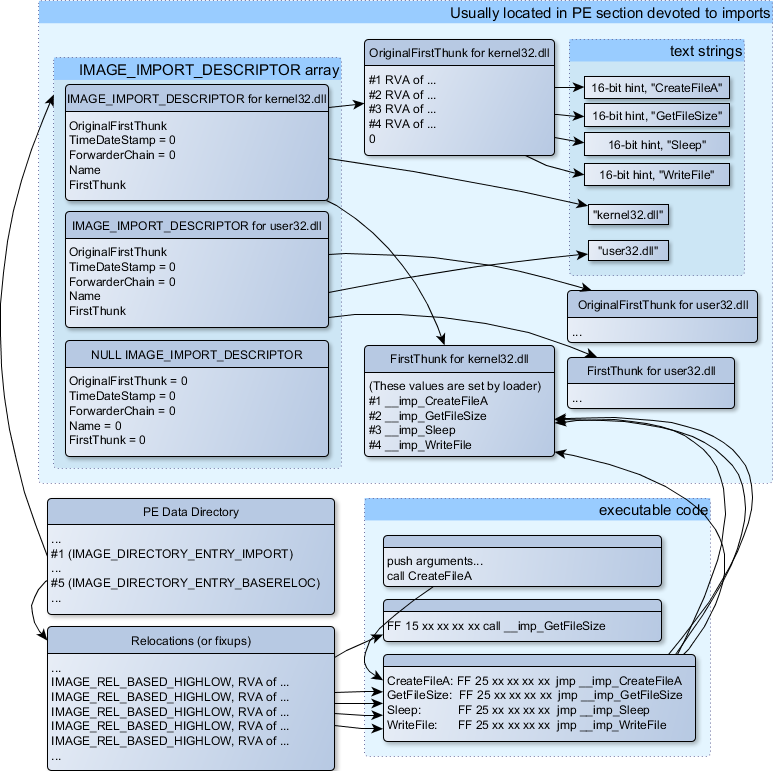
\includegraphics[scale=\FigScale]{OS/PE/unnamed0.png}
\caption{\RU{схема, объединяющая все структуры в PE-файлы, связанные с импортами}
\EN{A scheme that unites all PE-file structures related to imports}}
\end{figure}

\RU{Самая главная структура\EMDASH{}это массив}\EN{The main structure is the array} \IT{IMAGE\_IMPORT\_DESCRIPTOR}.
\RU{Каждый элемент на каждую импортируемую DLL}\EN{Each element for each DLL being imported}.

\RU{У каждого элемента есть}\EN{Each element holds the} \ac{RVA}\RU{-адрес}\EN{ address} 
\RU{текстовой строки (имя DLL)}\EN{of the text string (DLL name)} (\IT{Name}).

\IT{OriginalFirstThink} \RU{это}\EN{is the} \ac{RVA} \RU{-адрес таблицы \ac{INT}}\EN{address of the \ac{INT} table}. 
\RU{Это массив}\EN{This is an array of} 
\ac{RVA}\RU{-адресов}\EN{ addresses},
\RU{каждый из которых указывает на текстовую строку где записано имя функции}
\EN{each of which points to a text string with a function name}. 
\RU{Каждую строку предваряет 16-битное число}\EN{Each string is prefixed by a 16-bit integer} 
(\q{hint})\EMDASH\RU{\q{ординал} функции}\EN{\q{ordinal} of function}.

\RU{Если при загрузке удается найти функцию по ординалу, тогда сравнение текстовых строк не будет происходить.
Массив оканчивается нулем.}
\EN{While loading, if it is possible to find a function by ordinal,
then the strings comparison will not occur. The array is terminated by zero.}
\RU{Есть также указатель на таблицу \ac{IAT} с названием}
\EN{There is also a pointer to the \ac{IAT} table named} \IT{FirstThunk},
\RU{это просто}\EN{it is just the} \ac{RVA}\RU{-адрес}\EN{ address} 
\RU{места, где загрузчик будет проставлять адреса найденных функций}\EN{of the place where the loader
writes the addresses of the resolved functions}.

\RU{Места где загрузчик проставляет адреса, \IDA именует их так}
\EN{The points where the loader writes addresses are marked by \IDA like this}: \IT{\_\_imp\_CreateFileA}, \etc{}.

\RU{Есть по крайней мере два способа использовать адреса, проставленные загрузчиком}
\EN{There are at least two ways to use the addresses written by the loader}.

\begin{itemize}
\index{x86!\Instructions!CALL}
\item
\RU{В коде будут просто инструкции вроде}\EN{The code will have instructions like} 
\IT{call \_\_imp\_CreateFileA}, 
\RU{а так как, поле с адресом импортируемой функции это как бы глобальная переменная}
\EN{and since the field with the address of the imported function is a global variable in some sense}, 
\RU{то в таблице релоков добавляется адрес (плюс 1 или 2) в инструкции \IT{call}}
\EN{the address of the \IT{call} instruction (plus 1 or 2) is to be added to the relocs table},
\RU{на случай если модуль будет загружен по другому базовому адресу}
\EN{for the case when the module is loaded at a different base address}.

\RU{Но как видно, это приводит к увеличению таблицы релоков}\EN{But, obviously, this may enlarge
relocs table significantly}.
\RU{Ведь вызовов импортируемой функции у вас в модуле может быть очень много}
\EN{Because there are might be a lot of calls to imported functions in the module}.
\RU{К тому же, чем больше таблица релоков, тем дольше загрузка}
\EN{Furthermore, large relocs table slows down the process of loading modules}.

\index{x86!\Instructions!JMP}
\index{thunk-\RU{функции}\EN{functions}}
\item
\RU{На каждую импортируемую функцию выделяется только один переход на импортируемую функцию используя
инструкцию \JMP плюс релок на эту инструкцию}
\EN{For each imported function, there is only one jump allocated, using the \JMP instruction 
plus a reloc to it}.
\RU{Такие места-\q{переходники} называются также \q{thunk}-ами}\EN{Such points are also called \q{thunks}}.
\RU{А все вызовы импортируемой функции это просто инструкция \CALL на соответствующий \q{thunk}}
\EN{All calls to the imported functions are just \CALL instructions to the corresponding \q{thunk}}.
\RU{В данном случае, дополнительные релоки не нужны, потому что эти CALL-ы имеют относительный адрес,
и корректировать их не надо}\EN{In this case, additional relocs are not necessary because these CALL-s
have relative addresses and do not need to be corrected}.
\end{itemize}

\RU{Оба этих два метода могут комбинироваться}\EN{These two methods can be combined}.
\RU{Вероятно, линкер создает отдельный \q{thunk}, если вызовов слишком много, но по умолчанию\EMDASH{}не создает.}
\EN{Possible, the linker creates individual \q{thunk}s if there are too many calls to the function,
but not done by default.} \\
\\
\RU{Кстати, массив адресов функций, на который указывает FirstThunk,
не обязательно может быть в секции \ac{IAT}}\EN{By the way, the array of function addresses to which FirstThunk is
pointing is not necessary to be located in the \ac{IAT} section}.
\RU{К примеру, автор сих строк написал утилиту}\EN{For example, author of these lines once wrote the}
PE\_add\_import\footnote{\href{http://go.yurichev.com/17049}{yurichev.com}} 
\RU{для добавления импорта в уже существующий .exe-файл}\EN{utility for adding imports to an existing .exe-file}.
\RU{Раньше, в прошлых версиях утилиты, на месте функции, вместо которой вы хотите подставить вызов в другую DLL,
моя утилита вписывала такой код:}
\EN{Some time earlier, in the previous versions of the utility, 
at the place of the function you want to substitute with a call to another DLL,
my utility wrote the following code:}

\begin{lstlisting}
MOV EAX, [yourdll.dll!function]
JMP EAX
\end{lstlisting}

\RU{При этом, FirstThunk указывает прямо на первую инструкцию.
Иными словами, загрузчик, загружая yourdll.dll, 
прописывает адрес функции \IT{function} прямо в коде.}
\EN{FirstThunk points to the first instruction. In other words, when loading yourdll.dll,
the loader writes the address of the \IT{function} function right in the code.}

\RU{Надо также отметить что обычно секция кода защищена от записи}
\EN{It also worth noting that a
code section is usually write-protected}, \RU{так что, моя утилита
добавляет флаг}\EN{so my utility adds the} \\
\IT{IMAGE\_SCN\_MEM\_WRITE} 
\RU{для секции кода. Иначе при загрузке такой программы, она упадет с ошибкой}
\EN{flag for code section. Otherwise, the program to crash while loading with error code}
5 (access denied). \\
\\
\RU{Может возникнуть вопрос: а что если я поставляю программу с набором DLL,
которые никогда не будут меняться (в т.ч., адреса всех функций в этих DLL), может как-то можно ускорить процесс загрузки?}
\EN{One might ask: what if I supply a program with a set of DLL files which is not supposed to change (including addresses of all DLL functions),
is it possible to speed up the loading process?}

\RU{Да, можно прописать адреса импортируемых функций в массивы FirstThunk заранее}
\EN{Yes, it is possible to write the addresses of the functions to be imported into the FirstThunk arrays in advance}.
\RU{Для этого в структуре}\EN{The \IT{Timestamp} field is present in the} \\
\IT{IMAGE\_IMPORT\_DESCRIPTOR} \RU{имеется поле \IT{Timestamp}}\EN{structure}.
\RU{И если там присутствует какое-то значение, то загрузчик сверяет это значение с датой-временем DLL-файла}
\EN{If a value is present there, then the loader compares this value with the date-time of the DLL file}.
\RU{И если они равны, то загрузчик больше ничего не делает, и загрузка может происходить быстрее.}
\EN{If the values are equal, then the loader does not do anything, and the loading of the process can be faster.}
\RU{Это называется}\EN{This is called} \q{old-style binding}
\footnote{\href{http://go.yurichev.com/17050}{MSDN}.
\RU{Существует также}\EN{There is also the} \q{new-style binding}.}.
\index{BIND.EXE}
\RU{В Windows SDK для этого имеется утилита BIND.EXE}
\EN{The BIND.EXE utility in Windows SDK is for for this}.
\RU{Для ускорения загрузки вашей программы}\EN{For speeding up the loading of your program}, 
Matt Pietrek \InENRU \cite{Pietrek1}, \RU{предлагает делать binding сразу после инсталляции
вашей программы на компьютере конечного пользователя}\EN{suggests to do the binding shortly after your program
installation on the computer of the end user}. \\
\\
\RU{Запаковщики/зашифровщики PE-файлов могут также сжимать/шифровать таблицу импортов}
\EN{PE-files packers/encryptors may also compress/encrypt imports table}.
\RU{В этом случае, загрузчик Windows, конечно же, не загрузит все нужные DLL}
\EN{In this case, the Windows loader, of course, will not load all necessary DLLs}.
\index{Windows!Win32!LoadLibrary}
\index{Windows!Win32!GetProcAddress}
\RU{Поэтому распаковщик/расшифровщик делает это сам, при помощи вызовов}
\EN{Therefore, the packer/encryptor does this on its own, with the help of} 
\IT{LoadLibrary()} \AndENRU \EN{the }\IT{GetProcAddress()}\EN{ functions}.
\RU{Вот почему в запакованных файлах эти две функции часто присутствуют в \ac{IAT}.}
\EN{That is why these two functions are often present in \ac{IAT} in packed files.}\\
\\
\RU{В стандартных DLL входящих в состав Windows, часто, \ac{IAT} находится в самом начале PE-файла.}
\EN{In the standard DLLs from the Windows installation, \ac{IAT} often is located right in the beginning of the PE file.}
\RU{Возможно это для оптимизации}\EN{Supposedly, it is done for optimization}.
\RU{Ведь .exe-файл при загрузке не загружается в память весь 
(вспомните что инсталляторы огромного размера подозрительно быстро запускаются), он \q{мапится} (map), 
и подгружается в память частями по мере обращения к этой памяти.}
\EN{While loading, the .exe file is not loaded into memory as a whole (recall huge install programs which are
started suspiciously fast), it is \q{mapped}, and loaded into memory in parts as they are accessed.}
\RU{И возможно в Microsoft решили что так будет быстрее.}
\EN{Probably, Microsoft developers decided it will be faster.}

\subsection{\RU{Ресурсы}\EN{Resources}}

\label{PEresources}
\RU{Ресурсы в PE-файле\EMDASH{}это набор иконок, картинок, текстовых строк, описаний диалогов}
\EN{Resources in a PE file are just a set of icons, pictures, text strings, dialog descriptions}.
\RU{Возможно, их в свое время решили отделить от основного кода, чтобы все эти вещи были многоязычными,
и было проще выбирать текст или картинку того языка, который установлен в \ac{OS}}
\EN{Perhaps, they were separated from the main code, so all these things could be multilingual,
and it would be simpler to pick text or picture for the language that is currently set in the \ac{OS}}. \\
\\
\RU{В качестве побочного эффекта, их легко редактировать и сохранять обратно в исполняемый файл,
даже не обладая специальными знаниями, например, редактором ResHack}%
\EN{As a side effect, they can be edited easily and saved back to the executable file, even if one does not have special knowledge, 
by using the ResHack editor, for example} (\myref{ResHack}).

\subsection{.NET}

\index{.NET}
\RU{Программы на .NET компилируются не в машинный код, а в свой собственный байткод}
\EN{.NET programs are not compiled into machine code but into a special bytecode}.
\index{OEP}
\RU{Собственно, в .exe-файлы байткод вместо обычного кода, однако, точка входа (\ac{OEP}) 
указывает на крохотный фрагмент x86-кода}\EN{Strictly speaking, there is bytecode instead of the usual x86 code
in the .exe file, however, the entry point (\ac{OEP}) points to this tiny fragment of x86 code}:

\begin{lstlisting}
jmp         mscoree.dll!_CorExeMain
\end{lstlisting}

\RU{А в mscoree.dll и находится .NET-загрузчик, который уже сам будет работать с PE-файлом.}
\EN{The .NET loader is located in mscoree.dll, which processes the PE file.}
\index{Windows!Windows XP}
\RU{Так было в \ac{OS} до Windows XP. Начиная с XP, загрузчик \ac{OS} уже сам определяет, что это
.NET-файл и запускает его не исполняя этой инструкции \JMP}
\EN{It was so in all pre-Windows XP \ac{OS}es. Starting from XP, the \ac{OS} loader is able to detect the .NET file
and run it without executing that \JMP instruction}
\footnote{\href{http://go.yurichev.com/17051}{MSDN}}.

\index{TLS}
\subsection{TLS}

\RU{Эта секция содержит в себе инициализированные данные для}\EN{This section holds initialized
data for the} \ac{TLS}(\myref{TLS}) (\RU{если нужно}\EN{if needed}).
\RU{При старте нового треда, его}\EN{When a new thread start, its} 
\ac{TLS}\RU{-данные инициализируются данными из этой секции}
\EN{data is initialized using the data from this section}. \\
\\
\index{TLS!Callbacks}
\RU{Помимо всего прочего, спецификация PE-файла предусматривает инициализацию}
\EN{Aside from that, the PE file specification also provides initialization of the}
\ac{TLS}\RU{-секции, т.н.,}\EN{ section, the so-called} TLS callbacks.
\RU{Если они присутствуют, то они будут вызваны перед тем как передать управление на главную точку входа}
\EN{If they are present, they are to be called before the control is passed to the main entry point} (\ac{OEP}).
\RU{Это широко используется запаковщиками/защифровщиками PE-файлов.}
\EN{This is used widely in the PE file packers/encryptors.}

\subsection{\RU{Инструменты}\EN{Tools}}

\begin{itemize}
\item
\index{objdump}
\index{Cygwin}
objdump (\RU{имеется в}\EN{present in} cygwin) \RU{для вывода всех структур PE-файла}\EN{for dumping all PE-file structures}.

\item
\index{Hiew}
Hiew(\myref{Hiew}) \RU{как редактор}\EN{as editor}.

\item
	pefile\EMDASH{}Python-\RU{библиотека для работы с PE-файлами}\EN{library for PE-file processing}
\footnote{\url{http://go.yurichev.com/17052}}.

\item
\label{ResHack}
ResHack \acs{AKA} Resource Hacker\EMDASH{}\RU{редактор ресурсов}\EN{resources editor}
\footnote{\url{http://go.yurichev.com/17052}}.

\item
	PE\_add\_import\footnote{\url{http://go.yurichev.com/17049}}\EMDASH{}
\RU{простая утилита для добавления символа/-ов в таблицу импортов PE-файла}
\EN{simple tool for adding symbol(s) to PE executable import table}.

\item
	PE\_patcher\footnote{\href{http://go.yurichev.com/17054}{yurichev.com}}\EMDASH{} 
\RU{простая утилита для модификации PE-файлов}\EN{simple tool for patching PE executables}.

\item
	PE\_search\_str\_refs\footnote{\href{http://go.yurichev.com/17055}{yurichev.com}}\EMDASH{} 
\RU{простая утилита для поиска функции в PE-файле, где используется некая текстовая строка}
\EN{simple tool for searching for a function in PE executables which use some text string}.
\end{itemize}

\subsection{Further reading}

% FIXME: bibliography per chapter or section
\begin{itemize}
\item
Daniel Pistelli\EMDASH{}The .NET File Format \footnote{\url{http://go.yurichev.com/17056}}
\end{itemize}


\section{Windows SEH}
\label{sec:SEH}
\myindex{Windows!Structured Exception Handling}

\newcommand{\HandlerFunction}{\RU{функция-обработчик}\EN{handler function}}
\newcommand{\MoreEntries}{\RU{остальные элементы}\EN{more entries}}
\newcommand{\FilterFunction}{\RU{функция-фильтр}\EN{filter function}}
\newcommand{\HandlerFinallyFunction}{\RU{функция-обработчик/finally-обработчик}\EN{handler/finally function}}
\newcommand{\ScopeTable}{\RU{таблица scope}\EN{scope table}}

% subsections
\EN{\subsection{Let's forget about MSVC}

In Windows, the \ac{SEH} is intended for exceptions handling, nevertheless, it is language-agnostic,
not related to \Cpp or \ac{OOP} in any way.

Here we are going to take a look at \ac{SEH} in its isolated (from C++ and MSVC extensions) form.

\myindex{Windows!TIB}
\myindex{Windows!Win32!RaiseException()}

Each running process has a chain of \ac{SEH} handlers, \ac{TIB} has the address of the last handler.

When an exception occurs (division by zero, incorrect address access, user exception triggered by
calling the \TT{RaiseException()} function), the \ac{OS} finds the last handler in the \ac{TIB} and calls it,
passing all information about the \ac{CPU} state (register values, \etc{}) at the moment of the exception.

The exception handler considering the exception, was it made for it?
If so, it handles the exception.

If not, it signals to the \ac{OS} that it
cannot handle it and the \ac{OS} calls the next handler in the chain,
until a handler which is able to handle the exception is be found.

At the very end of the chain there a standard handler that shows the well-known dialog box, informing the user about a
process crash, some technical information about the \ac{CPU} state at the time of the crash,
and offering to collect all information and send it to developers in Microsoft. 

\begin{figure}[H]
\centering
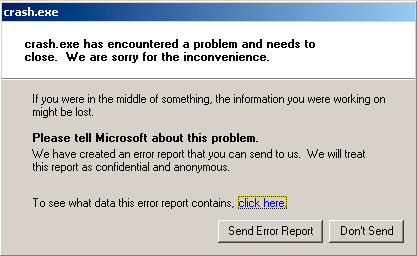
\includegraphics[scale=\NormalScale]{OS/SEH/1/crash_xp1.png}
\caption{Windows XP}
\end{figure}

\begin{figure}[H]
\centering
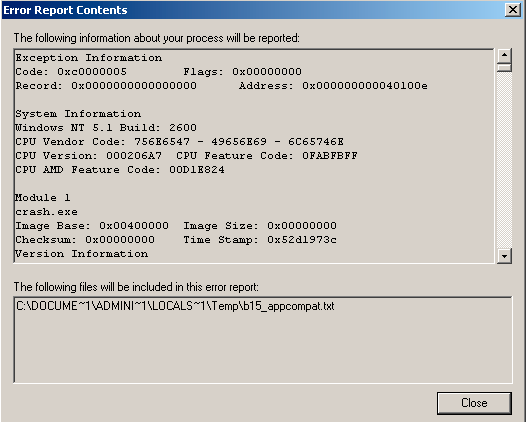
\includegraphics[scale=\NormalScale]{OS/SEH/1/crash_xp2.png}
\caption{Windows XP}
\end{figure}

\begin{figure}[H]
\centering
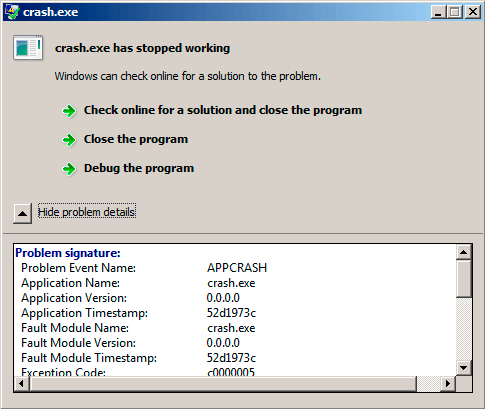
\includegraphics[scale=\NormalScale]{OS/SEH/1/crash_win7.png}
\caption{Windows 7}
\end{figure}

\begin{figure}[H]
\centering
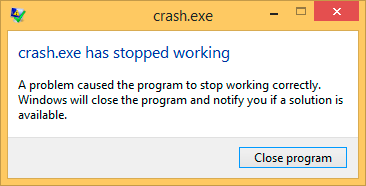
\includegraphics[scale=\NormalScale]{OS/SEH/1/crash_win81.png}
\caption{Windows 8.1}
\end{figure}

Earlier, this handler was called Dr. Watson
\footnote{\href{http://go.yurichev.com/17046}{wikipedia}}.

By the way, some developers make their own handler that sends information about the program crash to themselves.
\myindex{Windows!Win32!SetUnhandledExceptionFilter()}
It is registered with the help of \TT{SetUnhandledExceptionFilter()} 
and to be called if the \ac{OS} does not have any other way to handle the exception.
\myindex{\oracle}
An example is \oracle---it saves huge dumps containing all possible information about the \ac{CPU} and memory state.

Let's write our own primitive exception handler
\footnote{
	This example is based on the example from \cite{PietrekSEH}.
	It must be compiled with the SAFESEH option: 
	\TT{cl seh1.cpp /link /safeseh:no}
	More about SAFESEH here: \\
	\href{http://go.yurichev.com/17252}{MSDN}
}:
	
\lstinputlisting{OS/SEH/1/1.cpp}

The FS: segment register is pointing to the \ac{TIB} in win32.

The very first element in the \ac{TIB} is a pointer to the last handler in the chain.
We save it in the stack and store the address of our handler there.
The structure is named \TT{\_EXCEPTION\_REGISTRATION}, it is a simple singly-linked list and its elements are stored right in the stack.

\begin{lstlisting}[caption=MSVC/VC/crt/src/exsup.inc]
\_EXCEPTION\_REGISTRATION struc
     prev    dd      ?
     handler dd      ?
\_EXCEPTION\_REGISTRATION ends
\end{lstlisting}

So each \q{handler} field points to a handler and an each \q{prev} field points to the previous record in the stack.
The last record has \TT{0xFFFFFFFF} (-1) in the \q{prev} field.

\input{OS/SEH/1/tikz}

After our handler is installed, we call \TT{RaiseException()}
\footnote{\href{http://go.yurichev.com/17253}{MSDN}}.
This is an user exception. 
The handler checks the code.
If the code is \TT{0xE1223344}, it returning \TT{ExceptionContinueExecution},
which means that handler corrected the CPU state (it is usually a correction of the EIP/ESP registers) and the \ac{OS} can resume the execution of the.
If you alter slightly the code so the handler returns \TT{ExceptionContinueSearch},

then the \ac{OS} will call the other handlers, and it's unlikely that one who can handle it will be found, since
no one will have any information about it (rather about its code).
You will see the standard Windows dialog about a process crash.

What is the difference between a system exceptions and a user one? Here are the system ones:

\begin{center}
\begin{tabular}{ | l | l | l | }
\hline
\HeaderColor as defined in WinBase.h & 
\HeaderColor as defined in ntstatus.h & 
\HeaderColor numerical value \\
\hline
EXCEPTION\_ACCESS\_VIOLATION          & STATUS\_ACCESS\_VIOLATION           & 0xC0000005 \\
\hline
EXCEPTION\_DATATYPE\_MISALIGNMENT     & STATUS\_DATATYPE\_MISALIGNMENT      & 0x80000002 \\
\hline
EXCEPTION\_BREAKPOINT                & STATUS\_BREAKPOINT                 & 0x80000003 \\
\hline
EXCEPTION\_SINGLE\_STEP               & STATUS\_SINGLE\_STEP                & 0x80000004 \\
\hline
EXCEPTION\_ARRAY\_BOUNDS\_EXCEEDED     & STATUS\_ARRAY\_BOUNDS\_EXCEEDED      & 0xC000008C \\
\hline
EXCEPTION\_FLT\_DENORMAL\_OPERAND      & STATUS\_FLOAT\_DENORMAL\_OPERAND     & 0xC000008D \\
\hline
EXCEPTION\_FLT\_DIVIDE\_BY\_ZERO        & STATUS\_FLOAT\_DIVIDE\_BY\_ZERO       & 0xC000008E \\
\hline
EXCEPTION\_FLT\_INEXACT\_RESULT        & STATUS\_FLOAT\_INEXACT\_RESULT       & 0xC000008F \\
\hline
EXCEPTION\_FLT\_INVALID\_OPERATION     & STATUS\_FLOAT\_INVALID\_OPERATION    & 0xC0000090 \\
\hline
EXCEPTION\_FLT\_OVERFLOW              & STATUS\_FLOAT\_OVERFLOW             & 0xC0000091 \\
\hline
EXCEPTION\_FLT\_STACK\_CHECK           & STATUS\_FLOAT\_STACK\_CHECK          & 0xC0000092 \\
\hline
EXCEPTION\_FLT\_UNDERFLOW             & STATUS\_FLOAT\_UNDERFLOW            & 0xC0000093 \\
\hline
EXCEPTION\_INT\_DIVIDE\_BY\_ZERO        & STATUS\_INTEGER\_DIVIDE\_BY\_ZERO     & 0xC0000094 \\
\hline
EXCEPTION\_INT\_OVERFLOW              & STATUS\_INTEGER\_OVERFLOW           & 0xC0000095 \\
\hline
EXCEPTION\_PRIV\_INSTRUCTION          & STATUS\_PRIVILEGED\_INSTRUCTION     & 0xC0000096 \\
\hline
EXCEPTION\_IN\_PAGE\_ERROR             & STATUS\_IN\_PAGE\_ERROR              & 0xC0000006 \\
\hline
EXCEPTION\_ILLEGAL\_INSTRUCTION       & STATUS\_ILLEGAL\_INSTRUCTION        & 0xC000001D \\
\hline
EXCEPTION\_NONCONTINUABLE\_EXCEPTION  & STATUS\_NONCONTINUABLE\_EXCEPTION   & 0xC0000025 \\
\hline
EXCEPTION\_STACK\_OVERFLOW            & STATUS\_STACK\_OVERFLOW             & 0xC00000FD \\
\hline
EXCEPTION\_INVALID\_DISPOSITION       & STATUS\_INVALID\_DISPOSITION        & 0xC0000026 \\
\hline
EXCEPTION\_GUARD\_PAGE                & STATUS\_GUARD\_PAGE\_VIOLATION       & 0x80000001 \\
\hline
EXCEPTION\_INVALID\_HANDLE            & STATUS\_INVALID\_HANDLE             & 0xC0000008 \\
\hline
EXCEPTION\_POSSIBLE\_DEADLOCK         & STATUS\_POSSIBLE\_DEADLOCK          & 0xC0000194 \\
\hline
CONTROL\_C\_EXIT                      & STATUS\_CONTROL\_C\_EXIT             & 0xC000013A \\
\hline
\end{tabular}
\end{center}

That is how the code is defined:

\begin{center}
\begin{bytefield}[bitwidth=0.03\linewidth]{32}
\bitheader[endianness=big]{31,29,28,27,16,15,0} \\
\bitbox{2}{\TT{S}} & 
\bitbox{1}{\TT{U}} &
\bitbox{1}{0} & 
\bitbox{12}{Facility code} &
\bitbox{16}{Error code}
\end{bytefield}
\end{center}

S is a basic status code: 
11---error;
10---warning;
01---informational;
00---success.
U---whether the code is user code.

That is why we chose 0xE1223344---E\textsubscript{16} (1110\textsubscript{2}) 0xE (1110b) 
mean this it is 1) user exception; 2) error.

But to be honest, this example works fine without these high bits.

Then we try to read a value from memory at address 0.

Of course, there is nothing at this address in win32, so an exception is raised.

The very first handler is to be called---yours, and it will know about it first, by checking
the code if it's equal to the \TT{EXCEPTION\_ACCESS\_VIOLATION} constant.

The code that's reading from memory at address 0 is looks like this:

\lstinputlisting[caption=MSVC 2010]{OS/SEH/1/1_fragment.asm}

Will it be possible to fix this error \q{on the fly} and to continue with program execution?

Yes, our exception handler can fix the \EAX value and let the \ac{OS} execute this instruction once again.
So that is what we do. \printf prints 1234, because after the execution of our handler \EAX is not 0,
but contains the address of the global variable \TT{new\_value}.
The execution will resume.

That is what is going on: the memory manager in the \ac{CPU} signals about an error, the the \ac{CPU} suspends the thread,
finds the exception handler in the Windows kernel, 
which, in turn, starts to call all handlers in the \ac{SEH} chain, one by one.

We use MSVC 2010 here, but of course, there is no any guarantee that \EAX will be used for this pointer.

This address replacement trick is showy, and we considering it here as an illustration of \ac{SEH}'s internals.
Nevertheless, it's hard to recall any case where it is used for \q{on-the-fly} error fixing.

Why SEH-related records are stored right in the stack instead of some other place?

Supposedly because the \ac{OS} is not needing to care about freeing this information, 
these records are simply disposed when the function finishes its execution.
\myindex{\CStandardLibrary!alloca()}
This is somewhat like alloca(): (\myref{alloca}).

}
\RU{\subsubsection{Забудем на время о MSVC}

\ac{SEH} в Windows предназначен для обработки исключений, тем не менее, с \Cpp и \ac{OOP} он никак не связан.
Здесь мы рассмотрим \ac{SEH} изолированно от Си++ и расширений MSVC.

\myindex{Windows!TIB}
\myindex{Windows!Win32!RaiseException()}
Каждый процесс имеет цепочку \ac{SEH}-обработчиков, и адрес последнего записан в \ac{TIB}.
Когда происходит исключение (деление на ноль, обращение по неверному адресу в памяти, 
пользовательское исключение, поднятое при помощи \TT{RaiseException()}),
\ac{OS} находит последний обработчик в \ac{TIB} и вызывает его, 
передав ему информацию о состоянии \ac{CPU} в момент исключения
(все значения регистров, итд.).
Обработчик выясняет, то ли это исключение, для которого он создавался?

Если да, то он обрабатывает исключение.
Если нет, то показывает \ac{OS} что он не может его обработать и \ac{OS} вызывает следующий обработчик
в цепочке, и так до тех пор, пока не найдется обработчик способный обработать исключение.

В самом конце цепочки находится стандартный обработчик, показывающий всем очень известное окно, 
сообщающее что процесс упал, 
сообщает также состояние \ac{CPU} в момент падения и позволяет собрать и отправить информацию обработчикам 
в Microsoft. 

\begin{figure}[H]
\centering
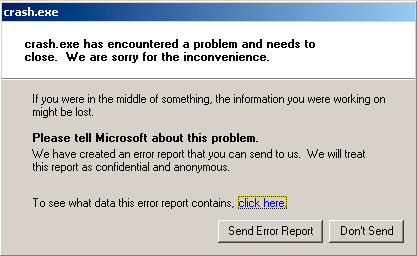
\includegraphics[width=0.6\textwidth]{OS/SEH/1/crash_xp1.png}
\caption{Windows XP}
\end{figure}

\begin{figure}[H]
\centering
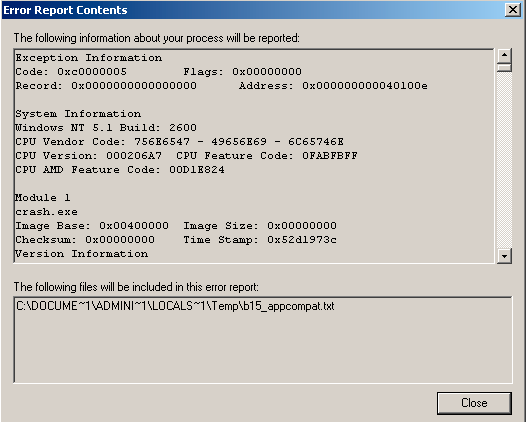
\includegraphics[width=0.6\textwidth]{OS/SEH/1/crash_xp2.png}
\caption{Windows XP}
\end{figure}

\begin{figure}[H]
\centering
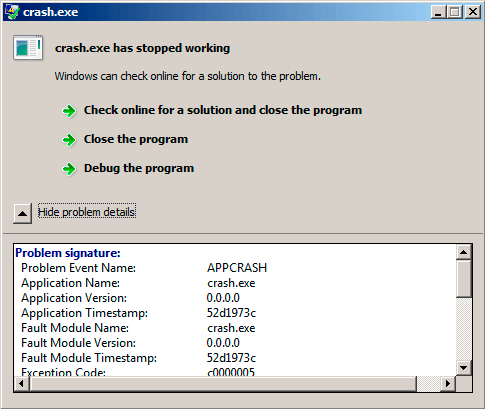
\includegraphics[width=0.6\textwidth]{OS/SEH/1/crash_win7.png}
\caption{Windows 7}
\end{figure}

\begin{figure}[H]
\centering
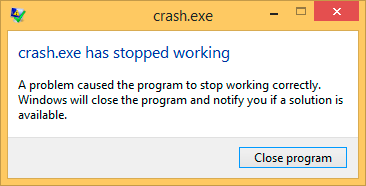
\includegraphics[width=0.6\textwidth]{OS/SEH/1/crash_win81.png}
\caption{Windows 8.1}
\end{figure}

Раньше этот обработчик назывался Dr. Watson
\footnote{\href{http://go.yurichev.com/17046}{wikipedia}}.

Кстати, некоторые разработчики делают свой собственный обработчик,
отправляющий информацию о падении программы им самим.\\
\myindex{Windows!Win32!SetUnhandledExceptionFilter()}
Он регистрируется при помощи функции \TT{SetUnhandledExceptionFilter()} 
и будет вызван если \ac{OS} не знает как иначе обработать исключение.

\myindex{\oracle}
А, например, \oracle в этом случае генерирует огромные дампы, 
содержащие всю возможную информацию и состоянии \ac{CPU} и памяти.

Попробуем написать свой примитивный обработчик исключений.
Этот пример основан на примере из \PietrekSEH.
Он должен компилироваться с опцией SAFESEH: \TT{cl seh1.cpp /link /safeseh:no}.
Подробнее об опции SAFESEH здесь: \href{http://go.yurichev.com/17252}{MSDN}.
	
\lstinputlisting{OS/SEH/1/1.cpp}

Сегментный регистр FS: в win32 указывает на \ac{TIB}.
Самый первый элемент \ac{TIB} это указатель на последний обработчик в цепочке.
Мы сохраняем его в стеке и записываем туда адрес своего обработчика.
Эта структура называется \TT{\_EXCEPTION\_REGISTRATION}, 
это простейший односвязный список, и эти элементы хранятся прямо в стеке.

\begin{lstlisting}[caption=MSVC/VC/crt/src/exsup.inc]
\_EXCEPTION\_REGISTRATION struc
     prev    dd      ?
     handler dd      ?
\_EXCEPTION\_REGISTRATION ends
\end{lstlisting}

Так что каждое поле \q{handler} указывает на обработчик,
а каждое поле \q{prev} указывает на предыдущую структуру в стеке.
Самая последняя структура имеет \TT{0xFFFFFFFF} (-1) в поле \q{prev}.

\input{OS/SEH/1/tikz}

После инсталляции своего обработчика, вызываем \TT{RaiseException()}\footnote{\href{http://go.yurichev.com/17253}{MSDN}}.
Это пользовательские исключения. 
Обработчик проверяет код.\\
Если код \TT{0xE1223344}, то он возвращает \TT{ExceptionContinueExecution},
что сигнализирует системе что обработчик скорректировал состояние CPU (обычно это регистры EIP/ESP) и что \ac{OS} может
возобновить исполнение треда.
Если вы немного измените код так что обработчик будет возвращать \TT{ExceptionContinueSearch},
то \ac{OS} будет вызывать остальные
обработчики в цепочке, и вряд ли найдется тот, кто обработает ваше исключение,
ведь информации о нем (вернее, его коде) ни у кого нет.
Вы увидите стандартное окно Windows о падении процесса.

Какова разница между системными исключениями и пользовательскими? Вот системные:

\small
\begin{center}
\begin{tabular}{ | l | l | l | }
\hline
\HeaderColor как определен в WinBase.h & 
\HeaderColor как определен в ntstatus.h & 
\HeaderColor численное значение \\
\hline
EXCEPTION\_ACCESS\_VIOLATION          & STATUS\_ACCESS\_VIOLATION           & 0xC0000005 \\
\hline
EXCEPTION\_DATATYPE\_MISALIGNMENT     & STATUS\_DATATYPE\_MISALIGNMENT      & 0x80000002 \\
\hline
EXCEPTION\_BREAKPOINT                & STATUS\_BREAKPOINT                 & 0x80000003 \\
\hline
EXCEPTION\_SINGLE\_STEP               & STATUS\_SINGLE\_STEP                & 0x80000004 \\
\hline
EXCEPTION\_ARRAY\_BOUNDS\_EXCEEDED     & STATUS\_ARRAY\_BOUNDS\_EXCEEDED      & 0xC000008C \\
\hline
EXCEPTION\_FLT\_DENORMAL\_OPERAND      & STATUS\_FLOAT\_DENORMAL\_OPERAND     & 0xC000008D \\
\hline
EXCEPTION\_FLT\_DIVIDE\_BY\_ZERO        & STATUS\_FLOAT\_DIVIDE\_BY\_ZERO       & 0xC000008E \\
\hline
EXCEPTION\_FLT\_INEXACT\_RESULT        & STATUS\_FLOAT\_INEXACT\_RESULT       & 0xC000008F \\
\hline
EXCEPTION\_FLT\_INVALID\_OPERATION     & STATUS\_FLOAT\_INVALID\_OPERATION    & 0xC0000090 \\
\hline
EXCEPTION\_FLT\_OVERFLOW              & STATUS\_FLOAT\_OVERFLOW             & 0xC0000091 \\
\hline
EXCEPTION\_FLT\_STACK\_CHECK           & STATUS\_FLOAT\_STACK\_CHECK          & 0xC0000092 \\
\hline
EXCEPTION\_FLT\_UNDERFLOW             & STATUS\_FLOAT\_UNDERFLOW            & 0xC0000093 \\
\hline
EXCEPTION\_INT\_DIVIDE\_BY\_ZERO        & STATUS\_INTEGER\_DIVIDE\_BY\_ZERO     & 0xC0000094 \\
\hline
EXCEPTION\_INT\_OVERFLOW              & STATUS\_INTEGER\_OVERFLOW           & 0xC0000095 \\
\hline
EXCEPTION\_PRIV\_INSTRUCTION          & STATUS\_PRIVILEGED\_INSTRUCTION     & 0xC0000096 \\
\hline
EXCEPTION\_IN\_PAGE\_ERROR             & STATUS\_IN\_PAGE\_ERROR              & 0xC0000006 \\
\hline
EXCEPTION\_ILLEGAL\_INSTRUCTION       & STATUS\_ILLEGAL\_INSTRUCTION        & 0xC000001D \\
\hline
EXCEPTION\_NONCONTINUABLE\_EXCEPTION  & STATUS\_NONCONTINUABLE\_EXCEPTION   & 0xC0000025 \\
\hline
EXCEPTION\_STACK\_OVERFLOW            & STATUS\_STACK\_OVERFLOW             & 0xC00000FD \\
\hline
EXCEPTION\_INVALID\_DISPOSITION       & STATUS\_INVALID\_DISPOSITION        & 0xC0000026 \\
\hline
EXCEPTION\_GUARD\_PAGE                & STATUS\_GUARD\_PAGE\_VIOLATION       & 0x80000001 \\
\hline
EXCEPTION\_INVALID\_HANDLE            & STATUS\_INVALID\_HANDLE             & 0xC0000008 \\
\hline
EXCEPTION\_POSSIBLE\_DEADLOCK         & STATUS\_POSSIBLE\_DEADLOCK          & 0xC0000194 \\
\hline
CONTROL\_C\_EXIT                      & STATUS\_CONTROL\_C\_EXIT             & 0xC000013A \\
\hline
\end{tabular}
\end{center}
\normalsize

Так определяется код:

\begin{center}
\begin{bytefield}[bitwidth=0.03\linewidth]{32}
\bitheader[endianness=big]{31,29,28,27,16,15,0} \\
\bitbox{2}{S} & 
\bitbox{1}{U} &
\bitbox{1}{0} & 
\bitbox{12}{Facility code} &
\bitbox{16}{Error code}
\end{bytefield}
\end{center}

S это код статуса: 
11 --- ошибка;
10 --- предупреждение;
01 --- информация;
00 --- успех.
U ---- является ли этот код пользовательским, а не системным.

Вот почему мы выбрали 0xE1223344 --- E\textsubscript{16} (1110\textsubscript{2}) 0xE (1110b)
означает что это 1) пользовательское исключение; 2) ошибка.
Хотя, если быть честным, этот пример нормально работает и без этих старших бит.

Далее мы пытаемся прочитать значение из памяти по адресу 0.
Конечно, в win32 по этому адресу обычно ничего нет, и сработает исключение.
Однако, первый обработчик, который будет заниматься этим делом\EMDASH{}ваш, и он узнает об этом
первым, проверяя код на соответствие с константной \TT{EXCEPTION\_ACCESS\_VIOLATION}.

А если заглянуть в то что получилось на ассемблере,
то можно увидеть, что код читающий из памяти по адресу 0, выглядит так:

\lstinputlisting[caption=MSVC 2010]{OS/SEH/1/1_fragment.asm}

Возможно ли \q{на лету} исправить ошибку и предложить программе исполняться далее?
Да, наш обработчик может изменить значение в \EAX и предложить \ac{OS} исполнить эту же инструкцию еще раз.
Что мы и делаем. \printf напечатает 1234, потому что после работы нашего обработчика, \EAX будет не 0,
а будет содержать адрес глобальной переменной \TT{new\_value}.
Программа будет исполняться далее.

Собственно, вот что происходит: срабатывает защита менеджера памяти в \ac{CPU}, 
он останавливает работу треда, отыскивает в ядре Windows обработчик исключений, 
тот, в свою очередь, начинает вызывать обработчики из цепочки \ac{SEH}, по одному.

Мы компилируем это всё в MSVC 2010, но конечно же, нет никакой гарантии 
что для указателя будет использован именно регистр \EAX.

Этот трюк с подменой адреса эффектно выглядит, и мы рассматриваем его здесь для наглядной иллюстрации работы \ac{SEH}.

Тем не менее, трудно припомнить, применяется ли где-то подобное на практике для исправления ошибок \q{на лету}.

Почему SEH-записи хранятся именно в стеке а не в каком-то другом месте?
Возможно, потому что \ac{OS} не нужно заботиться об освобождении этой информации, эти записи
просто пропадают как ненужные когда функция заканчивает работу.

\myindex{\CStandardLibrary!alloca()}
Это чем-то похоже на alloca(): (\myref{alloca}).

}
\EN{\subsection{Now let's get back to MSVC}

\myindex{\Cpp!exceptions}

Supposedly, Microsoft programmers needed exceptions in C, but not in \Cpp, so they added a non-standard C extension
to MSVC\footnote{\href{http://go.yurichev.com/17057}{MSDN}}.
It is not related to C++ \ac{PL} exceptions.

% FIXME russian listing:
\begin{lstlisting}
__try
{
    ...
}
__except(filter code)
{
    handler code
}
\end{lstlisting}

\q{Finally} block may be instead of handler code:

\begin{lstlisting}
__try
{
    ...
}
__finally
{
    ...
}
\end{lstlisting}


The filter code is an expression, telling whether this handler code corresponds to the exception raised.

If your code is too big and cannot fit into one expression, a separate filter function can be defined.\\
\\
There are a lot of such constructs in the Windows kernel.
Here are a couple of examples from there (\ac{WRK}):

\lstinputlisting[caption=WRK-v1.2/base/ntos/ob/obwait.c]{OS/SEH/2/wrk_ex1.c}

\lstinputlisting[caption=WRK-v1.2/base/ntos/cache/cachesub.c]{OS/SEH/2/wrk_ex2.c}

Here is also a filter code example:

\lstinputlisting[caption=WRK-v1.2/base/ntos/cache/copysup.c]{OS/SEH/2/wrk_ex3.c}

Internally, SEH is an extension of the OS-supported exceptions.
But the handler function is \TT{\_except\_handler3} (for SEH3) or \TT{\_except\_handler4} (for SEH4).

The code of this handler is MSVC-related, it is located in its libraries, or in msvcr*.dll.
It is very important to know that SEH is a MSVC thing.

Other win32-compilers may offer something completely different.

\subsubsection{SEH3}

SEH3 has \TT{\_except\_handler3} 
as a handler function, and extends the \TT{\_EXCEPTION\_REGISTRATION} table, adding
a pointer to the \IT{scope table} and \IT{previous try level} variable.
SEH4 extends the \IT{scope table} 
by 4 values for buffer overflow protection.\\
\\
The \IT{scope table} is a table that consists of pointers to the filter and handler code blocks, for each nested level of \IT{try/except}.

\input{OS/SEH/2/tikz}

Again, it is very important to understand that the \ac{OS} takes care only of the \IT{prev/handle} fields, and nothing more.
It is the job of the \TT{\_except\_handler3} function to read the other fields and \IT{scope table}, and decide
which handler to execute and when.\\
\\
\myindex{Wine}
\myindex{ReactOS}
The source code of the \TT{\_except\_handler3} function is closed.

However, Sanos OS, which has a win32 compatibility layer, has the same
functions reimplemented, which are somewhat equivalent to those in Windows
\footnote{\url{http://go.yurichev.com/17058}}.
Another reimplementation is present in 
Wine\footnote{\href{http://go.yurichev.com/17059}{GitHub}}
and ReactOS\footnote{\url{http://go.yurichev.com/17060}}.\\
\\
If the \IT{filter} pointer is NULL, the \IT{handler} 
pointer is the pointer to the \IT{finally} code block.\\
\\
During execution, the \IT{previous try level} value in the stack changes, so
\TT{\_except\_handler3} can get information about the current level of nestedness, 
in order to know which \IT{scope table} entry to use.

\subsubsection{SEH3: one try/except block example}

\lstinputlisting{OS/SEH/2/2.c}

\lstinputlisting[caption=MSVC 2003]{OS/SEH/2/2_SEH3.asm}

Here we see how the SEH frame is constructed in the stack.
The \IT{scope table} is located in the \TT{CONST} segment---indeed, these fields are not to be changed.
An interesting thing is how the \IT{previous try level} variable has changed.
The initial value is \TT{0xFFFFFFFF} ($-1$).
The moment when the body of the \TT{try} 
statement is opened is marked with an instruction that writes 0 to the variable.
The moment when the body of the \TT{try} statement is closed, $-1$ 
is written back to it.
We also see the addresses of filter and handler code.

Thus we can easily see the structure of the \IT{try/except} constructs in the function.\\
\\
Since the SEH setup code in the function prologue may be shared between many functions,
sometimes the compiler inserts a call to the \TT{SEH\_prolog()} function in the prologue, which does just that.

The SEH cleanup code is in the \TT{SEH\_epilog()} function.\\
\\
Let's try to run this example in \tracer{}:
\myindex{tracer}

\begin{lstlisting}
tracer.exe -l:2.exe --dump-seh
\end{lstlisting}

\begin{lstlisting}[caption=tracer.exe output]
EXCEPTION_ACCESS_VIOLATION at 2.exe!main+0x44 (0x401054) ExceptionInformation[0]=1
EAX=0x00000000 EBX=0x7efde000 ECX=0x0040cbc8 EDX=0x0008e3c8
ESI=0x00001db1 EDI=0x00000000 EBP=0x0018feac ESP=0x0018fe80
EIP=0x00401054
FLAGS=AF IF RF
* SEH frame at 0x18fe9c prev=0x18ff78 handler=0x401204 (2.exe!_except_handler3)
SEH3 frame. previous trylevel=0
scopetable entry[0]. previous try level=-1, filter=0x401070 (2.exe!main+0x60) handler=0x401088 (2.exe!main+0x78)
* SEH frame at 0x18ff78 prev=0x18ffc4 handler=0x401204 (2.exe!_except_handler3)
SEH3 frame. previous trylevel=0
scopetable entry[0]. previous try level=-1, filter=0x401531 (2.exe!mainCRTStartup+0x18d) handler=0x401545 (2.exe!mainCRTStartup+0x1a1)
* SEH frame at 0x18ffc4 prev=0x18ffe4 handler=0x771f71f5 (ntdll.dll!__except_handler4)
SEH4 frame. previous trylevel=0
SEH4 header:	GSCookieOffset=0xfffffffe GSCookieXOROffset=0x0
		EHCookieOffset=0xffffffcc EHCookieXOROffset=0x0
scopetable entry[0]. previous try level=-2, filter=0x771f74d0 (ntdll.dll!___safe_se_handler_table+0x20) handler=0x771f90eb (ntdll.dll!_TppTerminateProcess@4+0x43)
* SEH frame at 0x18ffe4 prev=0xffffffff handler=0x77247428 (ntdll.dll!_FinalExceptionHandler@16)
\end{lstlisting}

We see that the SEH chain consists of 4 handlers.\\
\\
\myindex{CRT}
The first two are located in our example. Two?
But we made only one?
Yes, another one was set up in the \ac{CRT} function \TT{\_mainCRTStartup()}, and as it seems that it handles at least \ac{FPU} exceptions.
Its source code can found in the MSVC installation: \TT{crt/src/winxfltr.c}.\\
\\
The third is the SEH4 one in ntdll.dll, 
and the fourth handler is not MSVC-related and is located in ntdll.dll, and has a self-describing function name.\\
\\
As you can see, there are 3 types of handlers in one chain:

one is not related to MSVC at all (the last one) and two MSVC-related: SEH3 and SEH4.

\subsubsection{SEH3: two try/except blocks example}

\lstinputlisting{OS/SEH/2/3.c}

Now there are two \TT{try} blocks.
So the \IT{scope table} now has two entries, one for each block.
\IT{Previous try level} changes as execution flow enters or exits the \TT{try} block.

\lstinputlisting[caption=MSVC 2003]{OS/SEH/2/3_SEH3.asm}

If we set a breakpoint on the \printf{} function, which is called from the handler, 
we can also see how yet another SEH handler is added.

Perhaps it's another machinery inside the SEH handling process.
Here we also see our \IT{scope table} consisting of 2 entries.

\begin{lstlisting}
tracer.exe -l:3.exe bpx=3.exe!printf --dump-seh
\end{lstlisting}

\begin{lstlisting}[caption=tracer.exe output]
(0) 3.exe!printf
EAX=0x0000001b EBX=0x00000000 ECX=0x0040cc58 EDX=0x0008e3c8
ESI=0x00000000 EDI=0x00000000 EBP=0x0018f840 ESP=0x0018f838
EIP=0x004011b6
FLAGS=PF ZF IF
* SEH frame at 0x18f88c prev=0x18fe9c handler=0x771db4ad (ntdll.dll!ExecuteHandler2@20+0x3a)
* SEH frame at 0x18fe9c prev=0x18ff78 handler=0x4012e0 (3.exe!_except_handler3)
SEH3 frame. previous trylevel=1
scopetable entry[0]. previous try level=-1, filter=0x401120 (3.exe!main+0xb0) handler=0x40113b (3.exe!main+0xcb)
scopetable entry[1]. previous try level=0, filter=0x4010e8 (3.exe!main+0x78) handler=0x401100 (3.exe!main+0x90)
* SEH frame at 0x18ff78 prev=0x18ffc4 handler=0x4012e0 (3.exe!_except_handler3)
SEH3 frame. previous trylevel=0
scopetable entry[0]. previous try level=-1, filter=0x40160d (3.exe!mainCRTStartup+0x18d) handler=0x401621 (3.exe!mainCRTStartup+0x1a1)
* SEH frame at 0x18ffc4 prev=0x18ffe4 handler=0x771f71f5 (ntdll.dll!__except_handler4)
SEH4 frame. previous trylevel=0
SEH4 header:	GSCookieOffset=0xfffffffe GSCookieXOROffset=0x0
		EHCookieOffset=0xffffffcc EHCookieXOROffset=0x0
scopetable entry[0]. previous try level=-2, filter=0x771f74d0 (ntdll.dll!___safe_se_handler_table+0x20) handler=0x771f90eb (ntdll.dll!_TppTerminateProcess@4+0x43)
* SEH frame at 0x18ffe4 prev=0xffffffff handler=0x77247428 (ntdll.dll!_FinalExceptionHandler@16)
\end{lstlisting}

\subsubsection{SEH4}

\myindex{\BufferOverflow}
\myindex{Security cookie}
During a buffer overflow (\myref{subsec:bufferoverflow}) attack, the address of the \IT{scope table} 
can be rewritten, so starting from MSVC 2005, SEH3 was upgraded to SEH4 in order to have buffer overflow protection.
The pointer to the \IT{scope table} is now \glslink{xoring}{xored} with a \gls{security cookie}.
The \IT{scope table} was extended to have a header consisting of two pointers to \IT{security cookies}.

Each element has an offset inside the stack of another value: 
the address of the \gls{stack frame} (\EBP) \glslink{xoring}{xored} with the \TT{security\_cookie} , placed in the stack.

This value will be read during exception handling and checked for correctness.
The \IT{security cookie} in the stack is random each time, so hopefully a remote attacker can't predict it. \\
\\
The initial \IT{previous try level} is $-2$ \InENRU SEH4 instead of $-1$.

\def\SEHfour{1}
\input{OS/SEH/2/tikz}

Here are both examples compiled in MSVC 2012 with SEH4:

\lstinputlisting[caption=MSVC 2012: one try block example]{OS/SEH/2/2_SEH4.asm}

\lstinputlisting[caption=MSVC 2012: two try blocks example]{OS/SEH/2/3_SEH4.asm}

Here is the meaning of the \IT{cookies}: \TT{Cookie Offset} 
is the difference between the address of the saved EBP value in the stack
and the $EBP \oplus security\_cookie$ value in the stack.
\TT{Cookie XOR Offset} is an additional difference between the 
$EBP \oplus security\_cookie$ value and what is
stored in the stack.

If this equation is not true, the process is to halt due to stack corruption:

\begin{center}
$security\_cookie \oplus (CookieXOROffset + address\_of\_saved\_EBP) == stack[address\_of\_saved\_EBP + CookieOffset]$
\end{center}

If \TT{Cookie Offset} is $-2$, this implies that it is not present.

\myindex{tracer}
\IT{Cookies} checking is also implemented in my \tracer{},
see \href{http://go.yurichev.com/17061}{GitHub} for details.\\
\\
It is still possible to fall back to SEH3 in the compilers after 
(and including) MSVC 2005 by setting the \TT{/GS-} option,
however, the \ac{CRT} code use SEH4 anyway.

}
\RU{\subsection{Теперь вспомним MSVC}

\myindex{\Cpp!исключения}
Должно быть, программистам Microsoft были нужны исключения в Си, но не в \Cpp, так что они добавили нестандартное расширение Си в MSVC
\footnote{\href{http://go.yurichev.com/17057}{MSDN}}.
Оно не связано с исключениями в Си++.

% FIXME russian listing:
\begin{lstlisting}
__try
{
    ...
}
__except(filter code)
{
    handler code
}
\end{lstlisting}

Блок \q{finally} может присутствовать вместо код обработчика:

\begin{lstlisting}
__try
{
    ...
}
__finally
{
    ...
}
\end{lstlisting}

Код-фильтр --- это выражение, отвечающее на вопрос, соответствует ли код этого обработчика к поднятому исключению.
Если ваш код слишком большой и не помещается в одно выражение, отдельная функция-фильтр может быть определена.\\
\\
Таких конструкций много в ядре Windows.
Вот несколько примеров оттуда (\ac{WRK}):

\lstinputlisting[caption=WRK-v1.2/base/ntos/ob/obwait.c]{OS/SEH/2/wrk_ex1.c}

\lstinputlisting[caption=WRK-v1.2/base/ntos/cache/cachesub.c]{OS/SEH/2/wrk_ex2.c}

Вот пример кода-фильтра:

\lstinputlisting[caption=WRK-v1.2/base/ntos/cache/copysup.c]{OS/SEH/2/wrk_ex3.c}

Внутри, SEH это расширение исключений поддерживаемых OS.

Но функция обработчик теперь или \TT{\_except\_handler3} (для SEH3) или \TT{\_except\_handler4} (для SEH4).
Код обработчика от MSVC, расположен в его библиотеках, или же в  msvcr*.dll.
Очень важно понимать, что SEH это специфичное для MSVC.
Другие win32-компиляторы могут предлагать что-то совершенно другое.

\subsubsection{SEH3}

SEH3 имеет \TT{\_except\_handler3} как функцию-обработчик, и расширяет структуру \TT{\_EXCEPTION\_REGISTRATION} добавляя указатель на \IT{scope table}
и переменную \IT{previous try level}.
SEH4 расширяет \IT{scope table} добавляя еще 4 значения связанных с защитой от переполнения буфера.\\
\\
\IT{scope table} это таблица, состоящая из указателей на код фильтра и обработчика, для каждого уровня вложенности \IT{try/except}.

\input{OS/SEH/2/tikz}

И снова, очень важно понимать, что OS заботится только о полях \IT{prev/handle}, и больше ничего.
Это работа функции \TT{\_except\_handler3} читать другие поля, читать \IT{scope table} и решать, какой обработчик исполнять и когда.\\
\\
\myindex{Wine}
\myindex{ReactOS}
Исходный код функции \TT{\_except\_handler3} закрыт.
Хотя, Sanos OS, имеющая слой совместимости с win32, имеет некоторые функции написанные заново, которые
в каком-то смысле эквивалентны тем что в Windows
\footnote{\url{http://go.yurichev.com/17058}}.
Другие попытки реализации имеются в 
Wine\footnote{\href{http://go.yurichev.com/17059}{GitHub}}
и ReactOS\footnote{\url{http://go.yurichev.com/17060}}.\\
\\
Если указатель \IT{filter} ноль, \IT{handler} указывает на код \IT{finally} .\\
\\
Во время исполнения, значение \IT{previous try level} в стеке меняется, чтобы функция
\TT{\_except\_handler3} знала о текущем уровне вложенности, чтобы знать, какой элемент таблицы
\IT{scope table} использовать.

\subsubsection{SEH3: пример с одним блоком try/except}

\lstinputlisting{OS/SEH/2/2.c}

\lstinputlisting[caption=MSVC 2003]{OS/SEH/2/2_SEH3.asm}

Здесь мы видим, как структура SEH конструируется в стеке.
\IT{Scope table} расположена в сегменте \TT{CONST} --- действительно, эти поля не будут меняться.
Интересно, как меняется переменная \IT{previous try level}.
Исходное значение \TT{0xFFFFFFFF} ($-1$).
Момент, когда тело \TT{try} открывается, обозначен инструкцией, записывающей 0 в эту переменную.
В момент, когда тело \TT{try} закрывается, $-1$ возвращается в нее назад.
Мы также видим адреса кода фильтра и обработчика.
Так мы можем легко увидеть структуру конструкций \IT{try/except} в функции.\\
\\
Так как код инициализации SEH-структур в прологе функций может быть общим для нескольких функций, иногда компилятор
вставляет в прологе вызов функции \TT{SEH\_prolog()}, которая всё это делает.
А код для деинициализации SEH в функции \TT{SEH\_epilog()}.\\
\\
Запустим этот пример в \tracer{}:
\myindex{tracer}

\begin{lstlisting}
tracer.exe -l:2.exe --dump-seh
\end{lstlisting}

\begin{lstlisting}[caption=tracer.exe output]
EXCEPTION_ACCESS_VIOLATION at 2.exe!main+0x44 (0x401054) ExceptionInformation[0]=1
EAX=0x00000000 EBX=0x7efde000 ECX=0x0040cbc8 EDX=0x0008e3c8
ESI=0x00001db1 EDI=0x00000000 EBP=0x0018feac ESP=0x0018fe80
EIP=0x00401054
FLAGS=AF IF RF
* SEH frame at 0x18fe9c prev=0x18ff78 handler=0x401204 (2.exe!_except_handler3)
SEH3 frame. previous trylevel=0
scopetable entry[0]. previous try level=-1, filter=0x401070 (2.exe!main+0x60) handler=0x401088 (2.exe!main+0x78)
* SEH frame at 0x18ff78 prev=0x18ffc4 handler=0x401204 (2.exe!_except_handler3)
SEH3 frame. previous trylevel=0
scopetable entry[0]. previous try level=-1, filter=0x401531 (2.exe!mainCRTStartup+0x18d) handler=0x401545 (2.exe!mainCRTStartup+0x1a1)
* SEH frame at 0x18ffc4 prev=0x18ffe4 handler=0x771f71f5 (ntdll.dll!__except_handler4)
SEH4 frame. previous trylevel=0
SEH4 header:	GSCookieOffset=0xfffffffe GSCookieXOROffset=0x0
		EHCookieOffset=0xffffffcc EHCookieXOROffset=0x0
scopetable entry[0]. previous try level=-2, filter=0x771f74d0 (ntdll.dll!___safe_se_handler_table+0x20) handler=0x771f90eb (ntdll.dll!_TppTerminateProcess@4+0x43)
* SEH frame at 0x18ffe4 prev=0xffffffff handler=0x77247428 (ntdll.dll!_FinalExceptionHandler@16)
\end{lstlisting}

Мы видим, что цепочка SEH состоит из 4-х обработчиков.\\
\\
\myindex{CRT}
Первые два расположены в нашем примере. Два?
Но ведь мы же сделали только один?
Да, второй был установлен в \ac{CRT}-функции 
\TT{\_mainCRTStartup()}, и судя по всему, он обрабатывает как минимум исключения связанные с \ac{FPU}.
Его код можно посмотреть в инсталляции MSVC: \TT{crt/src/winxfltr.c}.\\
\\
Третий это SEH4 в ntdll.dll, и четвертый это обработчик, не имеющий отношения к MSVC, расположенный в ntdll.dll, имеющий \q{говорящее} название функции.\\
\\
Как видно, в цепочке присутствуют обработчики трех типов:
один не связан с MSVC вообще (последний) и два связанных с MSVC: SEH3 и SEH4.

\subsubsection{SEH3: пример с двумя блоками try/except}

\lstinputlisting{OS/SEH/2/3.c}

Теперь здесь два блока \TT{try}.
Так что \IT{scope table} теперь содержит два элемента, один элемент на каждый блок.
\IT{Previous try level} меняется вместе с тем, как исполнение доходит до очередного \TT{try}-блока, либо выходит из него.

\lstinputlisting[caption=MSVC 2003]{OS/SEH/2/3_SEH3.asm}

Если установить точку останова на функцию \printf{} вызываемую из обработчика,
мы можем увидеть, что добавился еще один SEH-обработчик.
Наверное, это еще какая-то дополнительная механика, скрытая внутри процесса обработки исключений.
Тут мы также видим \IT{scope table} состоящую из двух элементов.

\begin{lstlisting}
tracer.exe -l:3.exe bpx=3.exe!printf --dump-seh
\end{lstlisting}

\begin{lstlisting}[caption=tracer.exe output]
(0) 3.exe!printf
EAX=0x0000001b EBX=0x00000000 ECX=0x0040cc58 EDX=0x0008e3c8
ESI=0x00000000 EDI=0x00000000 EBP=0x0018f840 ESP=0x0018f838
EIP=0x004011b6
FLAGS=PF ZF IF
* SEH frame at 0x18f88c prev=0x18fe9c handler=0x771db4ad (ntdll.dll!ExecuteHandler2@20+0x3a)
* SEH frame at 0x18fe9c prev=0x18ff78 handler=0x4012e0 (3.exe!_except_handler3)
SEH3 frame. previous trylevel=1
scopetable entry[0]. previous try level=-1, filter=0x401120 (3.exe!main+0xb0) handler=0x40113b (3.exe!main+0xcb)
scopetable entry[1]. previous try level=0, filter=0x4010e8 (3.exe!main+0x78) handler=0x401100 (3.exe!main+0x90)
* SEH frame at 0x18ff78 prev=0x18ffc4 handler=0x4012e0 (3.exe!_except_handler3)
SEH3 frame. previous trylevel=0
scopetable entry[0]. previous try level=-1, filter=0x40160d (3.exe!mainCRTStartup+0x18d) handler=0x401621 (3.exe!mainCRTStartup+0x1a1)
* SEH frame at 0x18ffc4 prev=0x18ffe4 handler=0x771f71f5 (ntdll.dll!__except_handler4)
SEH4 frame. previous trylevel=0
SEH4 header:	GSCookieOffset=0xfffffffe GSCookieXOROffset=0x0
		EHCookieOffset=0xffffffcc EHCookieXOROffset=0x0
scopetable entry[0]. previous try level=-2, filter=0x771f74d0 (ntdll.dll!___safe_se_handler_table+0x20) handler=0x771f90eb (ntdll.dll!_TppTerminateProcess@4+0x43)
* SEH frame at 0x18ffe4 prev=0xffffffff handler=0x77247428 (ntdll.dll!_FinalExceptionHandler@16)
\end{lstlisting}

\subsubsection{SEH4}

\myindex{\BufferOverflow}
\myindex{Security cookie}
Во время атаки переполнения буфера (\myref{subsec:bufferoverflow})
адрес \IT{scope table} может быть перезаписан, так что начиная с MSVC 2005, SEH3 был дополнен защитой от переполнения буфера, до SEH4.
Указатель на \IT{scope table} теперь \glslink{xoring}{про-XOR-ен} с \gls{security cookie}.

\IT{Scope table} расширена, теперь имеет заголовок, содержащий 2 указателя на \IT{security cookies}.
Каждый элемент имеет смешение внутри стека на другое значение: это адрес \glslink{stack frame}{фрейма} (\EBP) также \glslink{xoring}{про-XOR-еный} с 
\TT{security\_cookie} расположенный в стеке.
Это значение будет прочитано во время обработки исключения и проверено на правильность.

\IT{Security cookie} в стеке случайное каждый раз, так что атакующий, как мы надеемся, не может предсказать его.\\
\\
Изначальное значение \IT{previous try level} это $-2$ в SEH4 вместо $-1$.

\def\SEHfour{1}
\input{OS/SEH/2/tikz}

Оба примера скомпилированные в MSVC 2012 с SEH4:

\lstinputlisting[caption=MSVC 2012: one try block example]{OS/SEH/2/2_SEH4.asm}

\lstinputlisting[caption=MSVC 2012: two try blocks example]{OS/SEH/2/3_SEH4.asm}

Вот значение \IT{cookies}: \TT{Cookie Offset} 
это разница между адресом записанного в стеке значения EBP и значения $EBP \oplus security\_cookie$ в стеке.
\TT{Cookie XOR Offset} это дополнительная разница между значением $EBP \oplus security\_cookie$ и тем что записано в стеке.
Если это уравнение не верно, то процесс остановится из-за разрушения стека:

\begin{center}
$security\_cookie \oplus (CookieXOROffset + address\_of\_saved\_EBP) == stack[address\_of\_saved\_EBP + CookieOffset]$
\end{center}

Если \TT{Cookie Offset} равно $-2$, это значит, что оно не присутствует.

\myindex{tracer}
Проверка \IT{cookies} также реализована в моем \tracer{},
смотрите \href{http://go.yurichev.com/17061}{GitHub} для деталей.\\
\\
Возможность переключиться назад на SEH3 все еще присутствует в компиляторах после (и включая) MSVC 2005, нужно включить
опцию \TT{/GS-}, впрочем, \ac{CRT}-код будет продолжать использовать SEH4.

}
\EN{\subsection{Windows x64}

\label{SEH_win64}

As you might think, it is not very fast to set up the SEH frame at each function prologue.
Another performance problem is changing the 
\IT{previous try level} value many times during the function's execution.

So things are changed completely in x64: now all pointers to \TT{try} blocks, filter and handler functions are stored
in another PE segment \TT{.pdata}, 
and from there the \ac{OS}'s exception handler takes all the information.

Here are the two examples from the previous section compiled for x64:

\lstinputlisting[caption=MSVC 2012]{OS/SEH/3/2_x64.asm}

\lstinputlisting[caption=MSVC 2012]{OS/SEH/3/3_x64.asm}

Read \cite{IgorSkochinsky} for more detailed information about this.

Aside from exception information, \TT{.pdata}
is a section that contains the addresses of almost all function starts and ends,
hence it may be useful for a tools targeted at automated analysis.


}
\RU{\subsection{Windows x64}

\label{SEH_win64}
Как видно, это не самая быстрая штука, устанавливать SEH-структуры в каждом прологе функции.
Еще одна проблема производительности --- это менять переменную 
\IT{previous try level} много раз в течении исполнении функции.
Так что в x64 всё сильно изменилось, теперь все указатели на \TT{try}-блоки, функции фильтров и обработчиков,
теперь записаны в другом PE-сегменте
 \TT{.pdata}, откуда обработчик исключений \ac{OS} берет всю информацию.

Вот два примера из предыдущей секции, скомпилированных для x64:

\lstinputlisting[caption=MSVC 2012]{OS/SEH/3/2_x64.asm}

\lstinputlisting[caption=MSVC 2012]{OS/SEH/3/3_x64.asm}

Смотрите \cite{IgorSkochinsky} для более детального описания.

Помимо информации об исключениях, секция \TT{.pdata} 
также содержит начала и концы почти всех функций, так что эту информацию можно использовать в каких-либо
утилитах, предназначенных для автоматизации анализа.

}

\subsection{\RU{Больше о}\EN{Read more about} SEH}

\PietrekSEH, \IgorSkochinsky.

\section{Windows NT: \RU{Критические секции}\EN{Critical section}}
\index{Windows}

\label{critical_sections}

\RU{Критические секции в любой \ac{OS} очень важны в мультитредовой среде, используются в основном
для обеспечения гарантии что только один тред будет иметь доступ к данным,
блокируя остальные треды и прерывания}
\EN{Critical sections in any \ac{OS} are very important in multithreaded environment,
mostly used for issuing a guarantee
that only one thread will access some data, while blocking other threads and interrupts}. \\
\\
\RU{Вот как объявлена структура}\EN{That is how} \TT{CRITICAL\_SECTION} 
\RU{объявлена в линейке OS}\EN{structure is declared in} \gls{Windows NT}\EN{ line OS}:

\begin{lstlisting}[caption=(Windows Research Kernel v1.2) public/sdk/inc/nturtl.h]
typedef struct _RTL_CRITICAL_SECTION {
    PRTL_CRITICAL_SECTION_DEBUG DebugInfo;

    //
    //  The following three fields control entering and exiting the critical
    //  section for the resource
    //

    LONG LockCount;
    LONG RecursionCount;
    HANDLE OwningThread;        // from the thread's ClientId->UniqueThread
    HANDLE LockSemaphore;
    ULONG_PTR SpinCount;        // force size on 64-bit systems when packed
} RTL_CRITICAL_SECTION, *PRTL_CRITICAL_SECTION;
\end{lstlisting}

\RU{Вот как работает ф-ция}\EN{That's is how} EnterCriticalSection()\EN{ function works}:

\index{x86!\Instructions!LOCK}
\begin{lstlisting}[caption=Windows 2008/ntdll.dll/x86 (begin)]
_RtlEnterCriticalSection@4

var_C           = dword ptr -0Ch
var_8           = dword ptr -8
var_4           = dword ptr -4
arg_0           = dword ptr  8

                mov     edi, edi
                push    ebp
                mov     ebp, esp
                sub     esp, 0Ch
                push    esi
                push    edi
                mov     edi, [ebp+arg_0]
                lea     esi, [edi+4] ; LockCount
                mov     eax, esi
                lock btr dword ptr [eax], 0
                jnb     wait ; jump if CF=0

loc_7DE922DD:
                mov     eax, large fs:18h
                mov     ecx, [eax+24h]
                mov     [edi+0Ch], ecx
                mov     dword ptr [edi+8], 1
                pop     edi
                xor     eax, eax
                pop     esi
                mov     esp, ebp
                pop     ebp
                retn    4

... skipped
\end{lstlisting}

\index{x86!\Instructions!BTR}
\index{x86!\Prefixes!LOCK}
\RU{Самая важная инструкция в этом фрагменте кода --- это}
\EN{The most important instruction in this code fragment is} \TT{BTR} 
(\RU{с префиксом}\EN{prefixed with} \TT{LOCK}): 
\RU{нулевой бит сохраняется в флаге CF и очищается в памяти}
\EN{the zeroth bit is stored in CF flag and cleared in memory}.
\RU{Это \glslink{atomic operation}{атомарная операция}}\EN{This is \gls{atomic operation}}, 
\RU{блокирующая доступ всех остальных процессоров
к этому значению в памяти (обратите внимание на префикс \TT{LOCK} перед инструкцией \TT{BTR}.}
\EN{blocking all other CPUs to access this piece of memory 
(take a notice of \TT{LOCK} prefix before \TT{BTR} instruction).}
\RU{Если бит в}\EN{If the bit at} \TT{LockCount} \RU{был}\EN{was} 1, 
\RU{хорошо, сбросить его и вернуться из ф-ции: мы в критической секции}
\EN{fine, reset it and return from the function: we are in critical section}.
\RU{Если нет ~--- критическая секция уже занята другим тредом, тогда ждем}
\EN{If not~---critical section is already occupied by other thread, then wait}. \\
\RU{Ожидание там сделано через вызов}\EN{Wait is done there using} WaitForSingleObject(). \\
\\
\RU{А вот как работает ф-ция}\EN{And here is how} LeaveCriticalSection()\EN{ function works}:

\begin{lstlisting}[caption=Windows 2008/ntdll.dll/x86 (begin)]
_RtlLeaveCriticalSection@4 proc near

arg_0           = dword ptr  8

                mov     edi, edi
                push    ebp
                mov     ebp, esp
                push    esi
                mov     esi, [ebp+arg_0]
                add     dword ptr [esi+8], 0FFFFFFFFh ; RecursionCount
                jnz     short loc_7DE922B2
                push    ebx
                push    edi
                lea     edi, [esi+4]    ; LockCount
                mov     dword ptr [esi+0Ch], 0
                mov     ebx, 1
                mov     eax, edi
                lock xadd [eax], ebx
                inc     ebx
                cmp     ebx, 0FFFFFFFFh
                jnz     loc_7DEA8EB7

loc_7DE922B0:
                pop     edi
                pop     ebx

loc_7DE922B2:
                xor     eax, eax
                pop     esi
                pop     ebp
                retn    4

... skipped
\end{lstlisting}

\index{x86!\Instructions!XADD}
\TT{XADD} \RU{это ``обменять и прибавить''}\EN{is ``exchange and add''}. 
\RU{В данном случае, это значит прибавить 1 к значению в \TT{LockCount}, сохранить результат
в регистре \TT{EBX}, и в то же время 1 записывается в \TT{LockCount}}
\EN{In this case, it summing \TT{LockCount} value and 1 and stores result in \TT{EBX} register, 
and at the same time 1 goes to \TT{LockCount}}.
\RU{Эта операция также атомарная, потому что также имеет префикс \TT{LOCK}, что означает, что другие CPU
или ядра CPU в системе не будут иметь доступа к этой ячейке памяти}
\EN{This operation is atomic since it is prefixed by \TT{LOCK} as well,
meaning that all other CPUs or CPU cores in system are blocked from accessing this point of memory}.

\RU{Префикс }\TT{LOCK} \RU{очень важен}\EN{prefix is very important}: 
\RU{два треда, каждый из которых работает на разных CPU или ядрах CPU, могут попытаться одновременно
войти в критическую секцию, одновременно модифицируя значение в памяти, и это может привести к
непредсказуемым результатам}
\EN{two threads, each of which working on separate CPUs or CPU cores may try to
enter critical section and to modify the value in memory simultaneously,
this will result in unpredictable behaviour}.

% TODO linux



\part{\RU{Инструменты}\EN{Tools}}

\chapter{\RU{Дизассемблер}\EN{Disassembler}}

\section{IDA}

\label{IDA}
\RU{Старая бесплатная версия доступна для скачивания}\EN{Older freeware version is available for downloading}
\footnote{\url{http://www.hex-rays.com/idapro/idadownfreeware.htm}}.

\ShortHotKeyCheatsheet: \ref{sec:IDA_cheatsheet}

\chapter{\RU{Отладчик}\EN{Debugger}}

\section{tracer}

\index{tracer}
\label{tracer}
\RU{Я использую}\EN{I use} \IT{tracer}\footnote{\url{http://yurichev.com/tracer-\LANG.html}}
\RU{вместо отладчика}\EN{instead of debugger}.

\RU{Со временем я отказался использовать отладчик, потому что все что мне нужно от него: это иногда подсмотреть 
какие-либо аргументы какой-либо функции во время исполнения или состояние регистров в определенном месте. 
Каждый раз загружать отладчик для этого это слишком, поэтому я написал очень простую утилиту \IT{tracer}. 
Она консольная, запускается из командной строки, позволяет перехватывать исполнение функций, 
ставить брякпойнты на произвольные места, смотреть состояние регистров, модифицировать их, и так далее.}
\EN{I stopped to use debugger eventually, since all I need from it is to spot a function's arguments while
execution, or registers' state at some point.
To load debugger each time is too much, so I wrote a small utility \IT{tracer}.
It has console-interface, working from command-line, enable us to intercept function execution,
set breakpoints at arbitrary places, spot registers' state, modify it, etc.}

\RU{Но для учебы, очень полезно трассировать код руками в отладчике, наблюдать как меняются значения регистров 
(например, как минимум классический SoftICE, OllyDbg, WinDbg подсвечивают измененные регистры), 
флагов, данные, менять их самому, смотреть реакцию, и т.д.}
\EN{However, as for learning purposes, it is highly advisable to trace code in debugger manually, watch how register's state
changing (e.g. classic SoftICE, OllyDbg, WinDbg highlighting changed registers), flags, data, change them
manually, watch reaction, etc.}

\section{\olly}
\index{\olly}

\RU{Очень популярный отладчик пользовательской среды win32}\EN{Very popular user-mode win32 debugger}:\\
\url{http://www.ollydbg.de/}.

\ShortHotKeyCheatsheet: \label{sec:Olly_cheatsheet}

\section{GDB}
\index{GDB}

\RU{Не очень популярный отладчик у реверсеров, тем не менее, крайне удобный}\EN{Not very popular
debugger among reverse engineers, but very comfortable nevertheless}.
\RU{Некоторые команды}\EN{Some commands}: \ref{sec:GDB_cheatsheet}.

\chapter{\RU{Трассировка системных вызовов}\EN{System calls tracing}}

\label{strace}
\index{strace}
\index{dtruss}
\subsection{strace / dtruss}

\index{syscalls}
\RU{Позволяет показать, какие системные вызовы (syscalls(\ref{syscalls})) прямо сейчас вызывает процесс}
\EN{Will show which system calls (syscalls(\ref{syscalls})) are called by process right now}.
\RU{Например}\EN{For example}:

\begin{lstlisting}
# strace df -h

...

access("/etc/ld.so.nohwcap", F_OK)      = -1 ENOENT (No such file or directory)
open("/lib/i386-linux-gnu/libc.so.6", O_RDONLY|O_CLOEXEC) = 3
read(3, "\177ELF\1\1\1\0\0\0\0\0\0\0\0\0\3\0\3\0\1\0\0\0\220\232\1\0004\0\0\0"..., 512) = 512
fstat64(3, {st_mode=S_IFREG|0755, st_size=1770984, ...}) = 0
mmap2(NULL, 1780508, PROT_READ|PROT_EXEC, MAP_PRIVATE|MAP_DENYWRITE, 3, 0) = 0xb75b3000
\end{lstlisting}

\index{\MacOSX}
\RU{В \MacOSX для этого же имеется dtruss}\EN{\MacOSX has dtruss for the same aim}.

\index{cygwin}
\RU{В Cygwin также есть strace, впрочем, если я верно понял, 
он показывает результаты только для .exe-файлов скомпилированных для среды самого cygwin}
\EN{The Cygwin also has strace, but if I understood correctly, it works only for .exe-files
compiled for cygwin environment itself}.

\chapter{\RU{Декомпиляторы}\EN{Decompilers}}

\RU{Пока существует только один, публично доступный, декомпилятор в Си высокого качества}
\EN{There are only one known, publically available, high-quality decompiler to C code}: Hex-Rays:\\
\url{https://www.hex-rays.com/products/decompiler/}

% TODO Java, .NET, VB, etc

\chapter{\RU{Прочие инструменты}\EN{Other tools}}

\begin{itemize}
\item
Microsoft Visual Studio Express\footnote{\url{http://www.microsoft.com/express/Downloads/}}:
\RU{Усеченная бесплатная версия Visual Studio, пригодная для простых экспериментов}
\EN{Stripped-down free Visual Studio version, convenient for simple experiments}.
Some useful options: \ref{sec:MSVC_options}.

\item
\label{Hiew}
Hiew\footnote{\url{http://www.hiew.ru/}} \RU{для мелкой модификации кода в исполняемых файлах}
\EN{for small modifications of code in binary files}.

\item
\index{binary grep}
binary grep: \RU{небольшая утилита для поиска констант (либо просто последовательности байт)
в большом  кол-ве файлов, включая неисполняемые: \BGREPURL.}
\EN{the small utility for constants searching (or just any byte sequence) in a big pile of files, 
including non-executable: \BGREPURL.}
\end{itemize}


\chapter{\RU{Примеры из практики}\EN{Examples from practice}}

%\clearpage
\begin{center}
\vspace*{\fill}

\begin{figure}[H]
\centering
\myincludegraphics{cover4.jpg}
\end{figure}

\vspace*{\fill}
\end{center}

\clearpage

% sections here
\chapter{\EN{Task manager practical joke}\RU{Шутка с task manager} (Windows Vista)}

\RU{У меня только 4 ядра в процессоре в компьютере, так что Task Manager в Windows показывает только 4
графика загрузки процессора.}
\EN{I have only 4 CPU cores on my computer, so the Windows Task Manager shows only 4 CPU load graphs.}

\RU{Посмотрим, сможем ли мы немного хакнуть Task Manager, чтобы он находил больше ядер в компьютере.}
\EN{Let's see if it's possible to hack Task Manager slightly so it would detect more CPU cores on a computer.}

\RU{В начале задумаемся, откуда Task Manager знает количество ядер?}
\EN{Let us first think, how Task Manager would know number of cores?}
\RU{В win32 имеется ф-ция \TT{GetSystemInfo()}, при помощи которой можно узнать.}
\EN{There are \TT{GetSystemInfo()} win32 function present in win32 userspace which can tell us this.}
\RU{Но она не импортируется в}\EN{But it's not imported in} \TT{taskmgr.exe}.
\RU{Есть еще одна в \gls{NTAPI}, \TT{NtQuerySystemInformation()}, которая используется в 
\TT{taskmgr.exe} в ряде мест.}
\EN{There are, however, another one in \gls{NTAPI}, \TT{NtQuerySystemInformation()}, 
which is used in \TT{taskmgr.exe} in several places.}
\RU{Чтобы узнать количество ядер, нужно вызвать эту ф-цию с константной \TT{SystemBasicInformation} в 
первом аргументе (а это ноль}
\EN{To get number of cores, one should call this function with \TT{SystemBasicInformation} constant 
in first argument (which is zero}
\footnote{MSDN: \url{http://msdn.microsoft.com/en-us/library/windows/desktop/ms724509(v=vs.85).aspx}}).

\RU{Второй аргумент должен указывать на буфер, который примет всю информацию.}
\EN{Second argument should point to the buffer, which will receive all the information.}

\RU{Так что нам нужно найти все вызовы ф-ции \TT{NtQuerySystemInformation(0, ?, ?, ?)}.}
\EN{So we need to find all calls to the \TT{NtQuerySystemInformation(0, ?, ?, ?)} function.}
\RU{Откроем}\EN{Let's open} \TT{taskmgr.exe} \InENRU IDA. 
\RU{Что всегда хорошо с исполняемыми файлами от Microsoft, это то что IDA может скачать соответствующуий 
\gls{PDB}-файл именно для этого файла и добавить все имена ф-ций.}
\EN{What is always good about Microsoft executables is that IDA can download corresponding \gls{PDB} 
file for exactly this executable and add all function names.}
\RU{Видимо, Task Manager написан на C++ и некоторые ф-ции и классы имеют говорящие за себя имена.}
\EN{It seems, Task Manager written in C++ and some of function names and classes are really 
speaking for themselves.}
\RU{Тут есть классы}\EN{There are classes} CAdapter, CNetPage, CPerfPage, CProcInfo, CProcPage, CSvcPage, 
CTaskPage, CUserPage.
\RU{Должно быть, каждый класс соответствует каждой вкладке в Task Manager.}
\EN{Apparently, each class corresponding each tab in Task Manager.}

\RU{Я прошелся по всем вызовам и добавил комментарий с числом, передающимся как первый аргумент.}
\EN{I visited each call and I add comment with a value which is passed as the first function argument.}
\RU{В некоторых местах я написал ``not zero'', потому что значение в тех местах однозначно не ноль, 
но что-то другое (больше об этом во второй части главы).}
\EN{There are ``not zero'' I wrote at some places, because, the value there was not clearly zero, 
but something really different (more about this in the second part of this chapter).}
\RU{А мы все-таки ищем ноль передаваемый как аргумент.}
\EN{And we are looking for zero passed as argument after all.}

\begin{figure}[H]
\centering
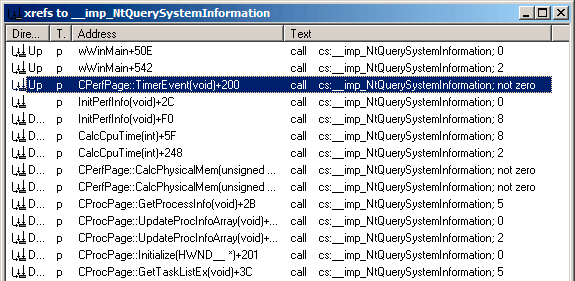
\includegraphics[scale=\FigScale]{examples/taskmgr/IDA_xrefs.png}
\caption{IDA: \RU{вызовы ф-ции}\EN{cross references to} NtQuerySystemInformation()}
\end{figure}

\RU{Да, имена действительно говорящие сами за себя.}
\EN{Yes, the names are really speaking for themselves.}

\RU{Когда я внимательно изучил каждое место, где вызывается \TT{NtQuerySystemInformation(0, ?, ?, ?)},
я быстро нашел то что нужно в ф-ции \TT{InitPerfInfo()}:}
\EN{When I closely investigating each place where \TT{NtQuerySystemInformation(0, ?, ?, ?)} is called,
I quickly found what I need in the \TT{InitPerfInfo()} function:}

\lstinputlisting[caption=taskmgr.exe (Windows Vista)]{examples/taskmgr/taskmgr.lst}

\TT{g\_cProcessors} \RU{это глобальная переменная и это имя присвоено IDA в соответствии с \gls{PDB}-файлом,
скачанным с сервера символов Microsoft}\EN{is a global variable, and this name was assigned by 
IDA according to \gls{PDB} loaded from the Microsoft symbol server}.

\RU{Байт берется из}\EN{The byte is taken from} \TT{var\_C20}. 
\RU{И}\EN{And} \TT{var\_C58} \RU{передается в}\EN{is passed to} \TT{NtQuerySystemInformation()} 
\RU{как указатель на принимающий буфер}\EN{as a pointer to the receiving buffer}.
\RU{Разница между}\EN{The difference between} 0xC20 \AndENRU 0xC58 \RU{это}\EN{is} 0x38 (56).
\RU{Посмотрим на формат структуры, который можно найти в MSDN:}
\EN{Let's take a look at returning structure format, which we can find in MSDN:}

\begin{lstlisting}
typedef struct _SYSTEM_BASIC_INFORMATION {
    BYTE Reserved1[24];
    PVOID Reserved2[4];
    CCHAR NumberOfProcessors;
} SYSTEM_BASIC_INFORMATION;
\end{lstlisting}

\RU{Это система x64, так что каждый PVOID занимает здесь 8 байт.}
\EN{This is x64 system, so each PVOID takes 8 byte here.}
\RU{Так что все \IT{reserved}-поля занимают $24+4*8=56$.}
\EN{So all \IT{reserved} fields in the structure takes $24+4*8=56$.}
\RU{О да, это значит что }\EN{Oh yes, this means, }\TT{var\_C20} \RU{в локальном стеке это именно поле}\EN{is the 
local stack is exactly} \TT{NumberOfProcessors} \RU{структуры}\EN{field of the} 
\TT{SYSTEM\_BASIC\_INFORMATION}\EN{ structure}.

\RU{Проверим, прав ли я}\EN{Let's check if I'm right}.
\RU{Скопируем}\EN{Copy} \TT{taskmgr.exe} \RU{из}\EN{from} \TT{C:\textbackslash{}Windows\textbackslash{}System32} 
\RU{в какую-нибудь другую папку}\EN{to some other folder} 
(\RU{чтобы}\EN{so the} \IT{Windows Resource Protection} \RU{не пыталась восстанавливать измененный}\EN{will not 
try to restore patched} \TT{taskmgr.exe}).

\RU{Откроем его в Hiew и найдем это место:}
\EN{Let's open it in Hiew and find the place:}

\begin{figure}[H]
\centering
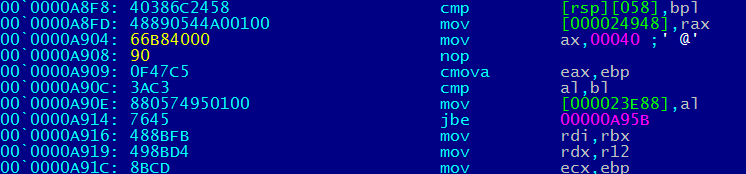
\includegraphics[scale=\FigScale]{examples/taskmgr/hiew1.png}
\caption{Hiew: \RU{найдем это место}\EN{find the place to be patched}}
\end{figure}

\RU{Заменим инструкцию \TT{MOVZX} на нашу.}
\EN{Let's replace \TT{MOVZX} instruction by our.}
\RU{Сделаем вид что у нас 64 ядра процессора}\EN{Let's pretend we've got 64 CPU cores}.
\RU{Добавим дополнительную инструкцию \ac{NOP} (потому что наша инструкция короче чем та что там сейчас):}
\EN{Add one additional \ac{NOP} (because our instruction is shorter than original one):}

\begin{figure}[H]
\centering
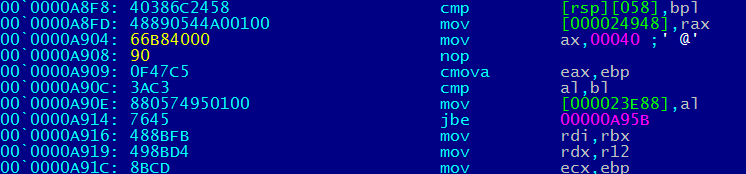
\includegraphics[scale=\FigScale]{examples/taskmgr/hiew1.png}
\caption{Hiew: \RU{меняем инструкцию}\EN{patch it}}
\end{figure}

\RU{И это работает}\EN{And it works}!
\RU{Конечно же, данные в графиках неправильные}\EN{Of course, data in graphs is not correct}.
\RU{Иногда, Task Manager даже показывает общую загрузку CPU более 100\%.}
\EN{At times, Task Manager even shows overall CPU load more than 100\%.}

\begin{figure}[H]
\centering
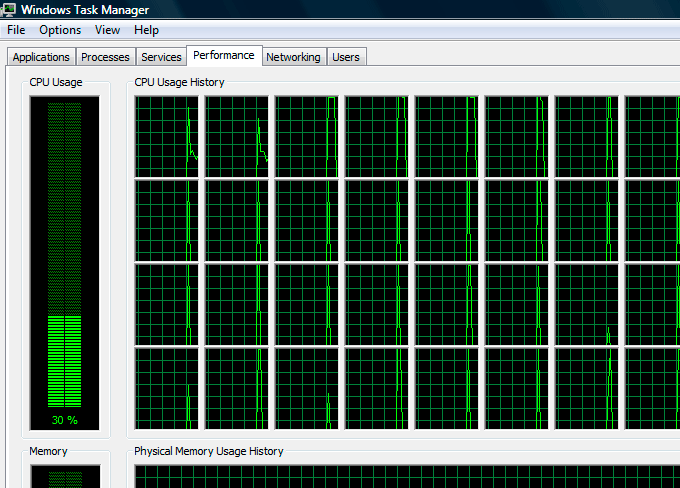
\includegraphics[scale=\FigScale]{examples/taskmgr/taskmgr_64cpu_crop.png}
\caption{\RU{Обманутый}\EN{Fooled} Windows Task Manager}
\end{figure}

\RU{Я выбрал число 64, потому что Task Manager падает если установить б\'{о}льшее значение.}
\EN{I picked number of 64, because Task Manager is crashing if you try to set larger value.}
\RU{Должно быть, Task Manager в Windows Vista не тестировался на компьютерах с большим количеством ядер.}
\EN{Apparently, Task Manager in Windows Vista was not tested on computer with larger count of cores.}
\RU{И наверное там есть внутри какие-то статичные структуры данных, ограниченные до 64-х ядер.}
\EN{So there are probably some static data structures inside it limited to 64 cores.}

\section{\RU{Использование LEA для загрузки значений}\EN{Using LEA to load values}}

\RU{Иногда, \TT{LEA} используется в \TT{taskmgr.exe} вместо \TT{MOV} для установки первого аргумента 
\TT{NtQuerySystemInformation()}:}
\EN{Sometimes, \TT{LEA} is used in \TT{taskmgr.exe} instead of \TT{MOV} to set first argument of 
\TT{NtQuerySystemInformation()}:}

\lstinputlisting[caption=taskmgr.exe (Windows Vista)]{examples/taskmgr/taskmgr2.lst}

\RU{Честно говоря, я не знаю почему, но \ac{MSVC} часто так делает.}
\EN{I honestly, don't know why, but that is what \ac{MSVC} often does.}
\RU{Может быть, это какая-то оптимизация и \TT{LEA} работает быстрее или лучше чем загрузка значения 
используя \TT{MOV}?}
\EN{Maybe this some kind of optiization and \TT{LEA} works faster or better than load 
value using \TT{MOV}?}

\clearpage
\chapterold{\RU{Шутка с игрой Color Lines}\EN{Color Lines game practical joke}}
\label{chap:color_lines}

\EN{This is a very popular game with several implementations in existence.
We can take one of them, called BallTriX, from 1997, available freely at \url{http://go.yurichev.com/17311}
\footnote{Or at \url{http://go.yurichev.com/17365} or \url{http://go.yurichev.com/17366}.}.
Here is how it looks:}%
\RU{Это очень популярная игра с большим количеством реализаций.
Возьмем одну из них, с названием BallTriX, от 1997, доступную бесплатно на \url{http://go.yurichev.com/17311}
\footnote{Или на \url{http://go.yurichev.com/17365} или \url{http://go.yurichev.com/17366}.}.
Вот как она выглядит:}

\begin{figure}[H]
\centering
\myincludegraphics{examples/lines/1.png}
\caption{\RU{Обычный вид игры}\EN{How this game looks usually}}
\label{fig:lines_1}
\end{figure}

\clearpage
\myindex{\CStandardLibrary!rand()}
\RU{Посмотрим, сможем ли мы найти генератор псевдослучайных чисел и и сделать с ним одну шутку.}
\EN{So let's see, is it be possible to find the random generator and do some trick with it.}
\IDA \RU{быстро распознает стандартную функцию}\EN{quickly recognize the standard} \TT{\_rand} \RU{в}\EN{function in} 
\TT{balltrix.exe} \RU{по адресу}\EN{at} \TT{0x00403DA0}.
\IDA \RU{также показывает, что она вызывается только из одного места}\EN{also shows that it is called 
only from one place}:

\lstinputlisting{examples/lines/random.lst}

\RU{Назовем её}\EN{We'll call it} \q{random}.
\RU{Пока не будем концентрироваться на самом коде функции}\EN{Let's not to dive into this function's code yet}.

\RU{Эта функция вызывается из трех мест}\EN{This function is referred from 3 places}.

\RU{Вот первые два}\EN{Here are the first two}:

\lstinputlisting{examples/lines/1.lst}

\EN{Here is the third one}\RU{Вот третье}:

\lstinputlisting{examples/lines/2.lst}

\RU{Так что у функции только один аргумент}\EN{So the function has only one argument}.
\RU{10 передается в первых двух случаях и 5 в третьем.}
\EN{10 is passed in first two cases and 5 in third.}
\RU{Мы также можем заметить, что размер доски 10*10 и здесь 5 возможных цветов}\EN{We can also notice 
that the board has a size of 10*10 and there are 5 possible colors}.
\RU{Это оно}\EN{This is it}!
\RU{Стандартная функция}\EN{The standard} \TT{rand()} \RU{возвращает число в пределах}\EN{function returns 
a number in the} \TT{0..0x7FFF} \RU{и это неудобно, так что многие программисты пишут свою функцию,
возвращающую случайное число в некоторых заданных пределах}\EN{range and this is often inconvenient,
so many programmers implement their own random functions which returns a random number in a specified range}.
\RU{В нашем случае, предел это}\EN{In our case, the range is} $0..n-1$ \AndENRU $n$ \RU{передается как
единственный аргумент в функцию}\EN{is passed as the sole argument of the function}.
\RU{Мы можем быстро проверить это в отладчике}\EN{We can quickly check this in any debugger}.

\RU{Сделаем так, чтобы третий вызов функции всегда возвращал ноль}\EN{So let's fix the third function call to always return zero}.
\RU{В начале заменим три инструкции}\EN{First, we will replace three instructions} (\TT{PUSH/CALL/ADD}) 
\RU{на}\EN{by} \ac{NOP}s.
\RU{Затем добавим инструкцию}\EN{Then we'll add} \INS{XOR EAX, EAX}\RU{, для очистки регистра \EAX}\EN{ instruction, 
to clear the \EAX register}.

\lstinputlisting{examples/lines/fixed.lst}

\RU{Что мы сделали, это заменили вызов функции}\EN{So what we did is we replaced a call to the} \TT{random()} 
\RU{на код, всегда возвращающий ноль}\EN{function by a code which always returns zero}.

\clearpage
\RU{Теперь запустим}\EN{Let's run it now}:

\begin{figure}[H]
\centering
\myincludegraphics{examples/lines/2.png}
\caption{\RU{Шутка сработала}\EN{Practical joke works}}
\end{figure}

\RU{О да, это работает}\EN{Oh yes, it works}\footnote{\RU{Автор этой книги однажды сделал это как 
шутку для его сотрудников, в надежде что они перестанут играть. 
Надежды не оправдались.}\EN{Author of this book once did this as a joke for his coworkers with 
the hope that they would stop playing. They didn't.}}.

\RU{Но почему аргументы функции}\EN{But why are the arguments to the} \TT{random()} \RU{это глобальные 
переменные}\EN{functions global variables}?
\RU{Это просто потому что в настройках игры можно изменять размер доски, так что эти параметры не 
фиксированы}\EN{That's just because it's possible to change the board size in the game's settings, 
so these values are not hardcoded}.
\EN{The }10 \AndENRU 5 \RU{это просто значения по умолчанию}\EN{values are just defaults}.

\chapter{\MinesweeperWinXPExampleChapterName}
\label{minesweeper_winxp}
\index{Windows!Windows XP}

\RU{Я не очень хорошо играю в Сапёра (Minesweeper), так что я попробую найти все скрытые мины в отладчике.}
\EN{I'm not very good at playing Minesweeper, so I'm going to reveal the hidden mines in the debugger.}

\index{\CStandardLibrary!rand()}
\index{Windows!PDB}
\RU{Как мы знаем, Сапёр располагает мины случайным образом, так что там должен быть генератор случайных чисел
или вызов стандартной функции Си \TT{rand()}.}
\EN{As we know, Minesweeper places mines randomly, so there has to be some kind of random number generator or
a call to the standard \TT{rand()} C-function.}
\RU{Вот что хорошо в реверсинге продуктов от Microsoft, так это то что часто есть \gls{PDB}-файл со всеми
символами (имена функций, \etc{}.).}
\EN{What is really cool about reversing Microsoft products is that there are \gls{PDB} 
file with symbols (function names, \etc{}).}
\RU{Когда я загружаю}\EN{When I load} \TT{winmine.exe} \RU{в}\EN{into} \IDA, \RU{она скачивает}\EN{it downloads the} 
\gls{PDB} \RU{файл именно для этого исполняемого файла и добавляет все имена}\EN{file exactly for this 
executable and shows all names}.

\RU{И вот оно, только один вызов}\EN{So here it is, the only call to} \TT{rand()} \RU{в этой 
функции}\EN{is this function}:

\begin{lstlisting}
.text:01003940 ; __stdcall Rnd(x)
.text:01003940 _Rnd@4          proc near               ; CODE XREF: StartGame()+53
.text:01003940                                         ; StartGame()+61
.text:01003940
.text:01003940 arg_0           = dword ptr  4
.text:01003940
.text:01003940                 call    ds:__imp__rand
.text:01003946                 cdq
.text:01003947                 idiv    [esp+arg_0]
.text:0100394B                 mov     eax, edx
.text:0100394D                 retn    4
.text:0100394D _Rnd@4          endp
\end{lstlisting}

\RU{Так её назвала \IDA и это было имя данное ей разработчиками Сапёра.}
\EN{\IDA named it so, and it was the name given to it by Minesweeper's developers.}

\RU{Функция очень простая}\EN{The function is very simple}:

\begin{lstlisting}
int Rnd(int limit)
{
    return rand() % limit;
};
\end{lstlisting}

\RU{(В \gls{PDB}-файле не было имени \q{limit}; это я назвал этот аргумент так.)}
\EN{(There was no \q{limit} name in the \gls{PDB} file; I named this argument.)}

\RU{Так что она возвращает случайное число в пределах от нуля до заданного предела}\EN{So it returns 
a random value from 0 to a specified limit}.

\TT{Rnd()} \RU{вызывается только из одного места, это функция с названием}\EN{is called only from one place, 
a function called} \TT{StartGame()}, 
\RU{и как видно, это именно тот код, что расставляет мины}\EN{and as it seems, this is exactly 
the code which place the mines}:

\begin{lstlisting}
.text:010036C7                 push    _xBoxMac
.text:010036CD                 call    _Rnd@4          ; Rnd(x)
.text:010036D2                 push    _yBoxMac
.text:010036D8                 mov     esi, eax
.text:010036DA                 inc     esi
.text:010036DB                 call    _Rnd@4          ; Rnd(x)
.text:010036E0                 inc     eax
.text:010036E1                 mov     ecx, eax
.text:010036E3                 shl     ecx, 5          ; ECX=ECX*32
.text:010036E6                 test    _rgBlk[ecx+esi], 80h
.text:010036EE                 jnz     short loc_10036C7
.text:010036F0                 shl     eax, 5          ; ECX=ECX*32
.text:010036F3                 lea     eax, _rgBlk[eax+esi]
.text:010036FA                 or      byte ptr [eax], 80h
.text:010036FD                 dec     _cBombStart
.text:01003703                 jnz     short loc_10036C7
\end{lstlisting}

\RU{Сапёр позволяет задать размеры доски, так что X (xBoxMac) и Y (yBoxMac) это глобальные переменные.}
\EN{Minesweeper allows you to set the board size, so the X (xBoxMac) and Y (yBoxMac) of the board are global variables.}
\RU{Они передаются в}\EN{They are passed to} \TT{Rnd()} \RU{и генерируются случайные координаты}\EN{and random 
coordinates are generated}.
\RU{Мина устанавливается инструкцией}\EN{A mine is placed by the} \TT{OR} \RU{на}\EN{instruction at} \TT{0x010036FA}. 
\RU{И если она уже была установлена до этого}\EN{And if it was placed before} 
(\RU{это возможно, если пара функций}\EN{it's possible if the pair of} \TT{Rnd()} 
\RU{сгенерирует пару, которая уже была сгенерирована}\EN{generates a coordinates pair which was already 
was generated}), 
\RU{тогда}\EN{then} \TT{TEST} \AndENRU \TT{JNZ} \RU{на}\EN{at} \TT{0x010036E6} 
\RU{перейдет на повторную генерацию пары}\EN{jumps to the generation routine again}.

\TT{cBombStart} \RU{это глобальная переменная, содержащая количество мин. Так что это цикл.}
\EN{is the global variable containing total number of mines. So this is loop.}

\RU{Ширина двухмерного массива это 32 (мы можем это вывести, глядя на инструкцию \TT{SHL}, которая умножает
одну из координат на 32)}\EN{The width of the array is 32 
(we can conclude this by looking at the \TT{SHL} instruction, which multiplies one of the coordinates by 32)}.

\RU{Размер глобального массива}\EN{The size of the} \TT{rgBlk} 
\RU{можно легко узнать по разнице между меткой}\EN{global array can be easily determined by the difference 
between the} \TT{rgBlk} 
\RU{в сегменте данных и следующей известной меткой}\EN{label in the data segment and the next known one}. 
\RU{Это}\EN{It is} 0x360 (864):

\begin{lstlisting}
.data:01005340 _rgBlk          db 360h dup(?)          ; DATA XREF: MainWndProc(x,x,x,x)+574
.data:01005340                                         ; DisplayBlk(x,x)+23
.data:010056A0 _Preferences    dd ?                    ; DATA XREF: FixMenus()+2
...
\end{lstlisting}

$864/32=27$.

\RU{Так что размер массива}\EN{So the array size is} $27*32$?
\RU{Это близко к тому что мы знаем: когда я попытался установить размер доски в установках Сапёра на}\EN{It is 
close to what we know: when I try to set board size to} $100*100$\RU{, то он установил размер}\EN{ in Minesweeper 
settings, it fallbacks to a board of size} $24*30$.
\RU{Так что это максимальный размер доски здесь}\EN{So this is the maximal board size here}.
\RU{И размер массива фиксирован для доски любого размера}\EN{And the array has a fixed size for any board size}.

\RU{Посмотрим на всё это в}\EN{So let's see all this in} \olly.
\RU{Я запустил Сапёр, присоединил (attach) \olly к нему и увидел содержимое памяти по адресу где массив}\EN{I ran 
Minesweeper, attaching \olly to it and I now see the memory dump at the address of the} 
\TT{rgBlk}\EN{ array}(\TT{0x01005340})
\footnote{\RU{Все адреса здесь для Сапёра под}\EN{All addresses here are for Minesweeper for} 
Windows XP SP3 English. 
\RU{Они могут отличаться для других сервис-паков}\EN{They may differ for other service packs}.}.

\RU{Так что у меня вышел такой дамп памяти массива}\EN{So I got this memory dump of the array}:

\lstinputlisting{examples/minesweeper/1.lst}

\olly, \RU{как и любой другой шестнадцатеричный редактор, показывает 16 байт на строку}\EN{like any other 
hexadecimal editor, shows 16 bytes per line}.
\RU{Так что каждая 32-байтная строка массива занимает ровно 2 строки}\EN{So each 32-byte array row occupies
exactly 2 lines here}.

\RU{Это уровень для начинающих (доска 9*9)}\EN{This is beginner level (9*9 board)}.

\RU{Тут еще какая-то квадратная структура, заметная визуально (байты 0x10)}\EN{There is some square 
structure can be seen visually (0x10 bytes)}.

\RU{Я нажал}\EN{I clicked} \q{Run} \InENRU \olly 
\RU{чтобы разморозить процесс Сапёра, потом нажал в случайное место окна Сапёра, попался на мине, но теперь
видны все мины}\EN{to unfreeze the Minesweeper process, then I clicked randomly at the Minesweeper window
and trapped into mine, but now I see all mines}:

\begin{figure}[H]
\centering
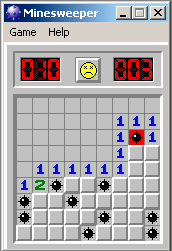
\includegraphics[scale=\FigScale]{examples/minesweeper/1.png}
\caption{\RU{Мины}\EN{Mines}}
\label{fig:minesweeper1}
\end{figure}

\RU{Сравнивая места с минами и дамп, мы можем обнаружить что 0x10 это граница, 0x0F\EMDASH{}пустой блок, 
0x8F\EMDASH{}мина.}
\EN{By comparing the mine places and the dump, we can conclude that 0x10 stands for border, 0x0F\EMDASH{}empty block, 0x8F---mine.}

\RU{Теперь я добавил комментариев и также включил все байты 0x8F в квадратные скобки:}
\EN{Now I added comments and also enclosed all 0x8F bytes into square brackets:}

\lstinputlisting{examples/minesweeper/2.lst}

\RU{Теперь я убрал все байты связанные с границами (0x10) и всё что за ними:}
\EN{Now I removed all \IT{border bytes} (0x10) and what's beyond those:}

\lstinputlisting{examples/minesweeper/3.lst}

\RU{Да, это всё мины, теперь это очень хорошо видно, в сравнении со скриншотом.}
\EN{Yes, these are mines, now it can be clearly seen and compared with the screenshot.}

\clearpage
\RU{Вот что интересно, это то что я могу модифицировать массив прямо в \olly.}
\EN{What is interesting is that I can modify the array right in \olly.}
\RU{Я убрал все мины заменив все байты 0x8F на 0x0F, и вот что у меня получилось в Сапёре}\EN{I removed 
all mines by changing all 0x8F bytes by 0x0F, and here is what I got in Minesweeper}:

\begin{figure}[H]
\centering
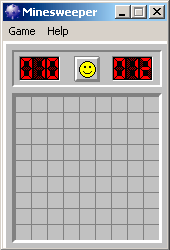
\includegraphics[scale=\FigScale]{examples/minesweeper/3.png}
\caption{\RU{Я убрал все мины в отладчике}\EN{I removed all mines in debugger}}
\label{fig:minesweeper3}
\end{figure}

\RU{Я также убрал их все и добавил их в первом ряду}\EN{I also moved all of them to the first line}: 

\begin{figure}[H]
\centering
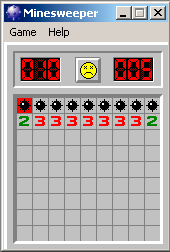
\includegraphics[scale=\FigScale]{examples/minesweeper/2.png}
\caption{\RU{Мины, установленные мною в отладчике}\EN{Mines I set in debugger}}
\label{fig:minesweeper2}
\end{figure}

\RU{Отладчик не очень удобен для подсматривания (а это была моя изначальная цель), так что я написал маленькую
утилиту для показа содержимого доски:}
\EN{Well, the debugger is not very convenient for eavesdropping (which was my goal anyway), so I wrote small utility
to dump the contents of the board:}

\lstinputlisting{examples/minesweeper/minesweeper_cheater.c}

\RU{Просто установите}\EN{Just set the} \ac{PID}
\footnote{PID \RU{можно увидеть в}\EN{it can be seen in} Task Manager 
(\RU{это можно включить в}\EN{enable it in} \q{View $\rightarrow$ Select Columns})} 
\RU{и адрес массива}\EN{and the address of the array} (\TT{0x01005340} \RU{для}\EN{for} Windows XP SP3 English) 
\RU{и она покажет его}\EN{and it will dump it}
\footnote{\RU{Скомпилированная версия здесь}\EN{The compiled executable is here}: 
\href{http://go.yurichev.com/17165}{beginners.re}}.

\RU{Она подключается к win32-процессу по \ac{PID}-у и просто читает из памяти процесса по этому адресу.}
\EN{It attaches itself to a win32 process by \ac{PID} and just reads process memory an the address.}

\section{\Exercises}

\begin{itemize}

\item \RU{Почему байты описывающие границы (0x10) присутствуют вообще?}
\EN{Why do the \IT{border bytes} (0x10) exist in the array?}
\RU{Зачем они нужны, если они вообще не видимы в интерфейсе Сапёра?}
\EN{What they are for if they are not visible in Minesweeper's interface?}
\RU{Как можно обойтись без них}\EN{How could it work without them}?

\item \RU{Как выясняется, здесь больше возможных значений (для открытых блоков, для тех на которых игрок установил
	флажок, \etc{}.).}
	\EN{As it turns out, there are more values possible (for open blocks, for flagged by user, \etc{}).}
\RU{Попробуйте найти значение каждого}\EN{Try to find the meaning of each one}.

\item \RU{Измените мою утилиту так, чтобы она в запущенном процессе Сапёра убирала все мины, 
или расставляла их в соответствии с каким-то заданным шаблоном.}
\EN{Modify my utility so it can remove all mines or set them in a fixed pattern that you want in the Minesweeper
process currently running.}

\item \RU{Измените мою утилиту так, чтобы она работала без задаваемого адреса массива и без \gls{PDB}-файла.}
\EN{Modify my utility so it can work without the array address specified and without a \gls{PDB} file.}
\RU{Да, вполне возможно автоматически найти информацию о доске в сегменте данных в запущенном процессе Сапёра.}
\EN{Yes, it's possible to find board information in the data segment of Minesweeper's running process automatically.}
\RU{Подсказка}\EN{Hint}: \myref{minesweeper_winxp_hint}.

\end{itemize}

\EN{\section{Hacking Windows clock}

Sometimes I did some kind of first April prank for my coworkers.

Let's find, if we could do something with Windows clock?
Can we force to go clock hands backwards?

First of all, when you click on date/time in status bar,\\
a \IT{C:\textbackslash{}WINDOWS\textbackslash{}SYSTEM32\textbackslash{}TIMEDATE.CPL} module gets executed,
which is usual executable PE file.

Let's see, how it draw hands?
When I open the file (from Windows 7) in Resource Hacker, there are clock faces, but with no hands:

\begin{figure}[H]
\centering
\myincludegraphics{examples/timedate/reshack.png}
\caption{Resource Hacker}
\end{figure}

OK, what we know? How to draw a clock hand? All they are started at the middle of circle, ending with its border.
Hence, we need to calculate coordinates of a point on circle's border.
From school-level mathematics we may remember that we need to use sine/cosine functions to draw circle, or at least
square root.
There are no such things in \IT{TIMEDATE.CPL}, at least at first glance.
But, thanks to Microsoft debugging PDB files, I can find a function named \IT{CAnalogClock::DrawHand()}, which calls
\IT{Gdiplus::Graphics::DrawLine()} at least twice.

Here is its code:

\lstinputlisting{examples/timedate/1.lst}

\myindex{Windows!Win32!MulDiv()}
We can see that \IT{DrawLine()} arguments are dependent on result of \IT{MulDiv()} function
and a \IT{table[]} table (name is mine),
which has 8-byte elements (look at \INS{LEA}'s second operand).

What is inside of table[]?

\lstinputlisting{examples/timedate/2.lst}

It's referenced only from \IT{DrawHand()} function at has 120 32-bit words or 60 32-bit pairs... wait, 60?
Let's take a closer look at these values.
First of all, I'll zap 6 pairs or 12 32-bit words with zeroes, and then I'll put patched \IT{TIMEDATE.CPL}
into \IT{C:\textbackslash{}WINDOWS\textbackslash{}SYSTEM32}.
(You may need to set owner of the *TIMEDATE.CPL* file to your primary user account (instead of \IT{TrustedInstaller}),
and also, boot in safe mode with command prompt so you can copy the file, which is usually locked.)

\begin{figure}[H]
\centering
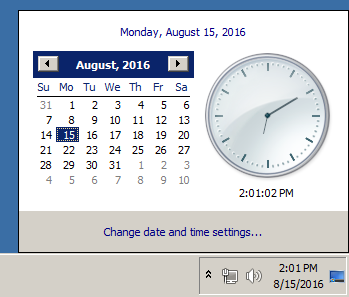
\includegraphics[width=0.5\textwidth]{examples/timedate/6_pairs_zeroed.png}
\caption{Attempt to run}
\end{figure}

Now when any hand is located at 0-5 seconds/minutes, it's invisible! However, opposite (shorter) part of second hand
is visible and moving.
When any hand is outside of this area, hand is visible as usual.

\myindex{Mathematica}
Let's take even closer look at the table in Mathematica.
I have copypasted table from the \IT{TIMEDATE.CPL} to a \IT{tbl} file (480 bytes).
We will take for granted the fact that these are signed values, because half of elements are below zero (0FFFFE0C1h, etc).
If these values would be unsigned, they would be suspiciously huge.

\begin{lstlisting}
In[]:= tbl = BinaryReadList["~/.../tbl", "Integer32"]

Out[]= {0, -7999, 836, -7956, 1663, -7825, 2472, -7608, 3253, -7308, 3999, \
-6928, 4702, -6472, 5353, -5945, 5945, -5353, 6472, -4702, 6928, \
-4000, 7308, -3253, 7608, -2472, 7825, -1663, 7956, -836, 8000, 0, \
7956, 836, 7825, 1663, 7608, 2472, 7308, 3253, 6928, 4000, 6472, \
4702, 5945, 5353, 5353, 5945, 4702, 6472, 3999, 6928, 3253, 7308, \
2472, 7608, 1663, 7825, 836, 7956, 0, 7999, -836, 7956, -1663, 7825, \
-2472, 7608, -3253, 7308, -4000, 6928, -4702, 6472, -5353, 5945, \
-5945, 5353, -6472, 4702, -6928, 3999, -7308, 3253, -7608, 2472, \
-7825, 1663, -7956, 836, -7999, 0, -7956, -836, -7825, -1663, -7608, \
-2472, -7308, -3253, -6928, -4000, -6472, -4702, -5945, -5353, -5353, \
-5945, -4702, -6472, -3999, -6928, -3253, -7308, -2472, -7608, -1663, \
-7825, -836, -7956}

In[]:= Length[tbl]
Out[]= 120
\end{lstlisting}

Let's treat two consecutive 32-bit values as pair:

\begin{lstlisting}
In[]:= pairs = Partition[tbl, 2]
Out[]= {{0, -7999}, {836, -7956}, {1663, -7825}, {2472, -7608}, \
{3253, -7308}, {3999, -6928}, {4702, -6472}, {5353, -5945}, {5945, \
-5353}, {6472, -4702}, {6928, -4000}, {7308, -3253}, {7608, -2472}, \
{7825, -1663}, {7956, -836}, {8000, 0}, {7956, 836}, {7825, 
1663}, {7608, 2472}, {7308, 3253}, {6928, 4000}, {6472, 
4702}, {5945, 5353}, {5353, 5945}, {4702, 6472}, {3999, 
6928}, {3253, 7308}, {2472, 7608}, {1663, 7825}, {836, 7956}, {0, 
7999}, {-836, 7956}, {-1663, 7825}, {-2472, 7608}, {-3253, 
7308}, {-4000, 6928}, {-4702, 6472}, {-5353, 5945}, {-5945, 
5353}, {-6472, 4702}, {-6928, 3999}, {-7308, 3253}, {-7608, 
2472}, {-7825, 1663}, {-7956, 836}, {-7999, 
0}, {-7956, -836}, {-7825, -1663}, {-7608, -2472}, {-7308, -3253}, \
{-6928, -4000}, {-6472, -4702}, {-5945, -5353}, {-5353, -5945}, \
{-4702, -6472}, {-3999, -6928}, {-3253, -7308}, {-2472, -7608}, \
{-1663, -7825}, {-836, -7956}}

In[]:= Length[pairs]
Out[]= 60
\end{lstlisting}

Let's try to treat each pair as X/Y coordinate and draw all 60 pairs, and also first 15 pairs:

\begin{figure}[H]
\centering
\myincludegraphics{examples/timedate/math.png}
\caption{Mathematica}
\end{figure}

Now this is something!
Each pair is just coordinate.
First 15 pairs are coordinates for $\frac{1}{4}$ of circle.

Perhaps, Microsoft developers precalculated all coordinates and put them into table.

Now I can understand why when I zapped 6 pairs, hands were invisible at that area: in fact, hands were drawed,
they just had zero length, because hand started at 0:0 coordinate and ended there.

\subsubsection{The prank (practical joke)}

Given all that, how would we force hands to go counterclockwise?
In fact, this is simple, we need just to rotate the table, so each hand, instead of drawing at place of first second,
would be drawing at place of 59th second.

I made the patcher a long time ago, at the very beginning of 2000s, for Windows 2000.
Hard to believe, it still works for Windows 7, perhaps, the table hasn't been changed since then!

Patcher source code: \url{https://github.com/dennis714/random_notes/blob/master/timedate/time_pt.c}.

Now I can see all hands goes backwards:

\begin{figure}[H]
\centering
\includegraphics[width=0.5\textwidth]{examples/timedate/counterclockwise.png}
\caption{Now it works}
\end{figure}

Well, there is no animation in this article, but if you look closer, you can see, that hands are in fact shows correct
time, but the whole clock face is rotated vertically, like we see it from the inside of clock.

\subsubsection{Windows 2000 leaked source code}

So I did the patcher and then Windows 2000 source code has been leaked (I can't force you to trust me, though).
Let's take a look on source code if that function and table.\\
The file is \IT{win2k/private/shell/cpls/utc/clock.c}:

\begin{lstlisting}
//
//  Array containing the sine and cosine values for hand positions.
//
POINT rCircleTable[] =
{
    { 0,     -7999},
    { 836,   -7956},
    { 1663,  -7825},
    { 2472,  -7608},
    { 3253,  -7308},
...
    { -4702, -6472},
    { -3999, -6928},
    { -3253, -7308},
    { -2472, -7608},
    { -1663, -7825},
    { -836 , -7956},
};

////////////////////////////////////////////////////////////////////////////
//
//  DrawHand
//
//  Draws the hands of the clock.
//
////////////////////////////////////////////////////////////////////////////

void DrawHand(
    HDC hDC,
    int pos,
    HPEN hPen,
    int scale,
    int patMode,
    PCLOCKSTR np)
{
    LPPOINT lppt;
    int radius;

    MoveTo(hDC, np->clockCenter.x, np->clockCenter.y);
    radius = MulDiv(np->clockRadius, scale, 100);
    lppt = rCircleTable + pos;
    SetROP2(hDC, patMode);
    SelectObject(hDC, hPen);

    LineTo( hDC,
            np->clockCenter.x + MulDiv(lppt->x, radius, 8000),
            np->clockCenter.y + MulDiv(lppt->y, radius, 8000) );
}
\end{lstlisting}

Now it's clear: coordinates has been precalculated as if clock face has height and width of $2 \cdot 8000$,
and then it's rescaled to current clock face radius using \IT{MulDiv()} function.

POINT structure\footnote{\url{https://msdn.microsoft.com/en-us/library/windows/desktop/dd162805(v=vs.85).aspx}}
is a structure of two 32-bit values, first is \IT{x}, second is \IT{y}.

}
\chapterold{\RU{Донглы}\EN{Dongles}}
\label{dongles}

\RU{Автор этих строк иногда делал замену \glslink{dongle}{донглам} или \q{эмуляторы донглов} 
и здесь немного примеров, как это происходит.}
\EN{The author of these lines, occasionally did software copy-protection \gls{dongle} replacements, or \q{dongle emulators} and here
are couple examples of how it's happening.}

\RU{Об одном неописанном здесь случае с Rockey и Z3 вы также можете прочитать здесь}
\EN{About one of the cases about Rocket and Z3 that is not present here, you can read here}:
\url{http://yurichev.com/tmp/SAT_SMT_DRAFT.pdf}.

\subsection{\IFRU{Пример}{Example} \#1: MacOS Classic \AndENRU PowerPC}

\index{PowerPC}
\index{Mac OS Classic}
\IFRU{Как-то я получил программу для}{I've got a program for} MacOS Classic
\footnote{\IFRU{MacOS перед тем как перейти на UNIX}{pre-UNIX MacOS}}, \IFRU{для}{for} PowerPC.
\IFRU{Компания, разработавшая этот продукт давно исчезла, так что (легальный) пользователь
боялся того что донгла может сломаться}{The company who developed the software product
was disappeared long time ago, so the (legal) customer was afraid of physical dongle damage}.

\IFRU{Если запустить программу без подключенной донглы, можно увидеть окно с надписью}
{While running without dongle connected, a message box with a text}
"Invalid Security Device"\IFRU{}{ appeared}.
\IFRU{Мне повезло потому что этот текст можно было легко найти внутри исполняемого файла}
{Luckily, this text string can be found easily in the executable binary file}.

\IFRU{Я не был знаком ни с Mac OS Classic, ни с PowerPC, но решил попробовать}
{I was not very familiar both with Mac OS Classic and PowerPC, but I tried anyway}.

\ac{IDA} \IFRU{открывает исполняемый файл легко, показывая его тип как}
{opens the executable file smoothly, reported its type as} 
"PEF (Mac OS or Be OS executable)" (\IFRU{действительно, это стандартный тип файлов в Mac OS Classic}
{indeed, it is a standard Mac OS Classic file format}).

\IFRU{В поисках текстовой строки с сообщение об ошибке, я попал на этот фрагмент кода}
{By searching for the text string with error message, I've got into this code fragment}:

\lstinputlisting{examples/dongles/1/1.lst}

\index{ARM}
\index{MIPS}
\IFRU{Да, это код PowerPC}{Yes, this is PowerPC code}.
\IFRU{Это очень типичный процессор для \ac{RISC} 1990-х}
{The CPU is very typical 32-bit \ac{RISC} of 1990s era}.
\IFRU{Каждая инструкция занимает 4 байта (как и в MIPS и ARM) и их имена немного похожи на имена 
инструкций MIPS}
{Each instruction occupies 4 bytes (just as in MIPS and ARM) and its names are somewhat resembling
MIPS instruction names}.

\TT{check1()} \IFRU{это имя которое я дал этой ф-ции позже}{is a function name I gave it to lately}.
\TT{BL} \IFRU{это инструкция}{is} \IT{Branch Link} 
\IFRU{т.е., предназначенная для вызова подпрограмм}{instruction, e.g., intended for subroutines calling}.
\IFRU{Самое важное место ~--- это инструкция \ac{BNE} срабатывающая если проверка наличия донглы прошла
успешно, либо не срабатывающая в случае ошибки: и тогда адрес текстовой строки с сообщением об ошибке
будет загружен в регистр r3 для последующей передачи в функцию отображения диалогового окна}
{The crucial point is \ac{BNE} instruction jumping if dongle protection check is passed 
or not jumping if error is occurred: 
then the address of the text string being loaded into r3 register for the subsequent passage into message box routine}.

\IFRU{Из}{From the} \cite{PPCABI} \IFRU{я узнал, что регистр r3 используется для возврата
значений (и еще r4 если значение 64-битное)}
{I've got to know the r3 register is used for values returning (and r4, in case of 64-bit values)}.

\index{x86!\Instructions!MOVZX}
\IFRU{Еще одна пока что неизвестная инструкция}{Another yet unknown instruction is} \TT{CLRLWI}. 
\IFRU{Из}{From} \cite{PPC} \IFRU{я узнал, что эта инструкция одновременно и очищает и загружает}{I've got to know that this instruction
do both clearing and loading}. 
\IFRU{В нашем случае, она очищает 24 старших бита из значения в r3 и записывает всё это в r0, 
так что это аналог}{In our case, it clears 24 high bits from the value in r3
and put it to r0, so it is analogical to} \MOVZX \InENRU x86 (\ref{movzx}),
\IFRU{но также устанавливает флаги, так что}{but it also sets the flags, so the} \ac{BNE} 
\IFRU{может проверить их потом}{can check them after}.

\IFRU{Посмотрим внутрь}{Let's take a look into} \TT{check1()}\IFRU{}{ function}:

\lstinputlisting{examples/dongles/1/check1.lst}

\IFRU{Как можно увидеть в \ac{IDA}, эта ф-ция вызывается из многих мест в программе, но только значение
в регистре r3 проверяется сразу после каждого вызова}
{As I can see in \ac{IDA}, that function is called from many places in program, but only r3 register value
is checked right after each call}.
\index{thunk-\IFRU{функции}{functions}}
\IFRU{Всё что эта ф-ция делает это только вызывает другую ф-цию, так что это}
{All this function does is calling other function, so it is} \gls{thunk function}: 
\IFRU{здесь присутствует и пролог ф-ции и эпилог, но регистр r3 не трогается, так что}
{there is function prologue and epilogue, but r3 register is not touched, so} \TT{checkl()} 
\IFRU{возвращает то, что возвращает}{returns what} \TT{check2()}\IFRU{}{ returns}.

\ac{BLR} \IFRU{это похоже возврат из ф-ции, но так как IDA делает всю разметку ф-ций автоматически,
наверное, мы можем пока не интересоваться этим}{is seems return from function, but since \ac{IDA} does functions layout, we probably do not need
to be interesting in this}.
\IFRU{Так как это типичный \ac{RISC}, похоже, подпрограммы вызываются используя}
{It seems, since it is a typical \ac{RISC}, subroutines are called using} \gls{link register},
\IFRU{точно как в}{just like in} ARM.

\IFRU{Ф-ция }{}\TT{check2()} \IFRU{более сложная}{function is more complex}:

\lstinputlisting{examples/dongles/1/check2.lst}

\IFRU{Снова повезло: имена некоторых ф-ций оставлены в исполняемом файле
(в символах в отладочной секции? Я не уверен, т.к. я не знаком с этим форматом файлов,
может быть это что-то вроде PE-экспортов (\ref{PE_exports_imports}))?
как например \TT{.RBEFINDNEXT()} and \TT{.RBEFINDFIRST()}.}
{I'm lucky again: some function names are leaved in the executable 
(debug symbols section? I'm not sure, since I'm not very familiar with the file format, maybe it is
some kind of PE exports? (\ref{PE_exports_imports})),
like \TT{.RBEFINDNEXT()} and \TT{.RBEFINDFIRST()}.}
\IFRU{В итоге, эти ф-ции вызывают другие ф-ции с именами вроде}
{Eventually these functions are calling other functions with names like} \TT{.GetNextDeviceViaUSB()}, 
\TT{.USBSendPKT()},
\IFRU{так что они явно работают с каким-то USB-устройством}{so these are clearly dealing with USB device}.

\IFRU{Тут даже есть ф-ция с названием}{There are even a function named} 
\TT{.GetNextEve3Device()}\EMDASH\IFRU{звучит знакомо, в 1990-х годах была донгла}{sounds familiar, there was} Sentinel Eve3 
\IFRU{для ADB-порта (присутствующих на Макинтошах)}{dongle for ADB port (present on Macs) in 1990s}.

\IFRU{В начале посмотрим на то как устанавливается регистр r3 одновременно игнорируя всё остальное}
{Let's first take a look on how r3 register is set before return simultaneously ignoring all we see}.
\IFRU{Мы знаем, что ``хорошее'' значение в r3 должно быть не нулевым, а нулевой r3 приведет
к выводу диалогового окна с сообщением об ошибке}
{We know that ``good'' r3 value should be non-zero, zero r3 will lead execution
flow to the message box with an error message}.

\IFRU{В ф-ции имеются две инструкции}{There are two instructions} \TT{li \%r3, 1} 
\IFRU{и одна}{present in the function and one} \TT{li \%r3, 0} 
(\IT{Load Immediate}, \IFRU{т.е., загрузить значение в регистр}{i.e., loading value into register}).
\IFRU{Самая первая инструкция находится на}{The very first instruction at} 
\TT{0x001186B0}\EMDASH\IFRU{и честно говоря, я не знаю что это означает, нужно больше времени на изучение ассемблера PowerPC}
{frankly speaking, I don't know
what it mean, I need some more time to learn PowerPC assembly language}.

\IFRU{А вот то что мы видим дальше понять проще}{What we see next is, however, easier to understand}: 
\IFRU{вызывается }{}\TT{.RBEFINDFIRST()} \IFRU{и в случае ошибки, 0 будет записан в r3
и мы перейдем на \IT{exit}, а иначе будет вызвана ф-ция \TT{check3()} ~--- если и она будет
выполнена с ошибкой, будет вызвана}{is called:
in case of its failure, 0 is written into r3 and we jump to \IT{exit}, otherwise another
function is called (\TT{check3()})~---if it is failing too, 
the} \TT{.RBEFINDNEXT()} \IFRU{вероятно, для поиска другого USB-устройства}
{is called, probably, in order to look for another USB device}.

N.B.: \TT{clrlwi. \%r0, \%r3, 16} \IFRU{это аналог того что мы уже видели, но она очищает 16 старших бит,
т.е.}{it is analogical to what we already saw, but it clears
16 bits, i.e.}, \TT{.RBEFINDFIRST()} \IFRU{вероятно возвращает 16-битное значение}
{probably returns 16-bit value}.

\TT{B} \IFRU{означает}{meaning} \IT{branch} \IFRU{~--- безусловный переход}{is unconditional jump}.

\ac{BEQ} \IFRU{это обратная инструкция от}{is inverse instruction of} \ac{BNE}.

\IFRU{Посмотрим на}{Let's see} \TT{check3()}:

\lstinputlisting{examples/dongles/1/check3.lst}

\IFRU{Здесь много вызовов}{There are a lot of calls to} \TT{.RBEREAD()}. 
\IFRU{Эта ф-ция вероятно читает какие-то значения из донглы, которые потом сравниваются здесь при помощи}
{The function is probably return some values from the dongle,
so they are compared here with hard-coded variables using} \TT{CMPLWI}.

\IFRU{Мы также видим в регистр r3 записывается перед каждым вызовом}
{We also see that r3 register is also filled before each call to} \TT{.RBEREAD()} 
\IFRU{одно из этих значений}{by one of these values}: 0, 1, 8, 0xA, 0xB, 0xC, 0xD, 4, 5.
\IFRU{Вероятно адрес в памяти или что-то в этом роде}{Probably memory address or something like that}?

\IFRU{Да, действительно, если погуглить имена этих ф-ций, можно легко найти документацию к}
{Yes, indeed, by googling these function names it is easy to find} Sentinel Eve3\IFRU{}{ dongle manual}!

\IFRU{Мне даже, наверное, не нужно изучать остальные инструкции PowerPC: всё что делает эта ф-ция это просто
вызывает}
{I probably even do not need to learn other PowerPC instructions: all this function does is just
calls} \TT{.RBEREAD()}, \IFRU{сравнивает его результаты с константами и возвращает 1 если результат сравнения положительный или 0 в другом случае}{compare its results with constants and returns 1 if comparisons
are fine or 0 otherwise}.

\IFRU{Всё ясно: \TT{check1()} должна всегда возвращать 1 или иное ненулевое значение}
{OK, all we've got is that \TT{check1()} should return always 1 or any other non-zero value}.
\IFRU{Но так как я не очень уверен в своих знаниях инструкций PowerPC, я буду осторожен и пропатчу
переходы в \TT{check2} на адресах}{But since I'm not very confident in PowerPC instructions,
I will be careful: I will patch
jumps in \TT{check2()} at} \TT{0x001186FC} \AndENRU \TT{0x00118718}.

\IFRU{На}{At} \TT{0x001186FC} \IFRU{я записал байты}{I wrote bytes} 0x48 \AndENRU 0 
\IFRU{таким образом превращая инструкцию}{thus converting} \ac{BEQ} 
\IFRU{в инструкцию}{instruction into} 
\TT{B} (\IFRU{безусловный переход}{unconditional jump}):
\IFRU{Я заметил этот опкод прямо в коде даже без обращения к}
{I spot its opcode in the code without even referring to} \cite{PPC}.

\IFRU{На}{At} \TT{0x00118718} \IFRU{я записал байт}{I wrote} 0x60 \AndENRU \IFRU{еще 3 нулевых байта,
таким образом превращая её в инструкцию}{3 zero bytes thus converting it to}
\ac{NOP}\IFRU{}{ instruction}:
\IFRU{Этот опкод я тоже подсмотрел прямо в коде}{I spot its opcode in the code too}.

\IFRU{Резюмируя, такие простые модификации можно делать в \ac{IDA} даже с минимальными знаниями
ассемблера}{Summarizing, such small modifications can be done with \ac{IDA} and minimal assembly language knowledge}.


\EN{\subsection{Example \#2: SCO OpenServer}

\label{examples_SCO}
\myindex{SCO OpenServer}
An ancient software for SCO OpenServer from 1997 
developed
by a company that disappeared a long time ago.


There is a special dongle driver to be installed in the system, that contains the following text strings:
\q{Copyright 1989, Rainbow Technologies, Inc., Irvine, CA}
\AndENRU
\q{Sentinel Integrated Driver Ver. 3.0 }.


After the installation of the driver in SCO OpenServer, these device files appear in the /dev filesystem:

\begin{lstlisting}
/dev/rbsl8
/dev/rbsl9
/dev/rbsl10
\end{lstlisting}


The program reports an error without dongle connected, but the error string cannot be found in the executables.

\myindex{COFF}

Thanks to \ac{IDA}, it is easy to load the COFF executable used in SCO OpenServer.

%
Let's also try to find \q{rbsl} string and indeed, found it in this code fragment:

\lstinputlisting{examples/dongles/2/1.lst}


Yes, indeed, the program needs to communicate with the driver somehow.

\myindex{thunk-functions}
The only place where the \TT{SSQC()}
function is called is the \gls{thunk function}:

\lstinputlisting{examples/dongles/2/2.lst}

SSQ() 
is called from at least 2 functions.

One of these is:

\lstinputlisting{examples/dongles/2/check1.lst}

\q{\TT{3C}} \AndENRU \q{\TT{3E}} 
sound familiar: there was a Sentinel Pro dongle by Rainbow with no memory,
providing only one crypto-hashing secret function.

You can read a short description
of what hash function is here: \myref{hash_func}.

But let's get back to the program.

So the program can only check the presence or absence of a connected dongle.

No other information can be written to such dongle, as it has no memory.
The two-character codes are commands
(we can see how the commands are handled in the 
\TT{SSQC()} function) 

and all other strings are hashed inside the dongle, being transformed into a 16-bit number.
The algorithm was secret,
so it was not possible to write a driver replacement or to remake the dongle hardware that would emulate it perfectly.

However, it is always possible to intercept all accesses to it and to find what constants
the hash function results are compared to.

But we need to say that it is possible to build a robust software copy protection scheme based on secret
cryptographic hash-function: let it encrypt/decrypt the data files your software uses.

But let's get back to the code.

Codes 51/52/53 
are used for LPT printer port selection.
3x/4x are used for \q{family} 
selection (that's how Sentinel Pro dongles are differentiated from each other: more than one
dongle can be connected to a LPT port).


The only non-2-character string passed to the hashing function is "0123456789".

Then, the result is compared against the set of valid results.

If it is correct, 0xC or 0xB is to be written into the global variable \TT{ctl\_model}.%


Another text string that gets passed is
"PRESS ANY KEY TO CONTINUE: ", but the result is not checked.
Hard to say why, probably by mistake
\footnote{
What a strange feeling: to find bugs in such ancient software.}.


Let's see where the value from the global variable \TT{ctl\_mode} is used.

One such place is:

\lstinputlisting{examples/dongles/2/4.lst}

If it is 0, an encrypted error message is passed to a decryption routine and printed.

\myindex{x86!\Instructions!XOR}

The error string decryption routine seems a simple \gls{xoring}:

\lstinputlisting{examples/dongles/2/err_warn.lst}

%
That's why we were unable to find the error messages in the executable files, because they are encrypted
(which is is popular practice).

Another call to the \TT{SSQ()} hashing function passes the
\q{offln} string to it and compares the result with
\TT{0xFE81} \AndENRU \TT{0x12A9}.

If they don't match, it works with some \TT{timer()} 
function (maybe waiting for a poorly
connected dongle to be reconnected and check again?) and then decrypts another error message to dump.

\lstinputlisting{examples/dongles/2/check2.lst}

Bypassing the dongle is pretty straightforward: just patch all jumps after the relevant \CMP instructions.


Another option is to write our own SCO OpenServer driver, containing a table of questions and answers, all of those which present in the program.

\subsubsection{Decrypting error messages}

By the way, we can also 
try to decrypt all error messages.
The algorithm that is located in the \TT{err\_warn()} 
function is very simple, indeed:

\lstinputlisting[caption=Decryption function]{examples/dongles/2/decrypting_EN.lst}

As we can see, 
not just string is supplied to the decryption function, but also the key:

\begin{lstlisting}
.text:0000DAF7 error:                                  ; CODE XREF: sync_sys+255j
.text:0000DAF7                                         ; sync_sys+274j ...
.text:0000DAF7                 mov     [ebp+var_8], offset encrypted_error_message2
.text:0000DAFE                 mov     [ebp+var_C], 17h ; decrypting key
.text:0000DB05                 jmp     decrypt_end_print_message

...

; this name we gave to label manually:
.text:0000D9B6 decrypt_end_print_message:              ; CODE XREF: sync_sys+29Dj
.text:0000D9B6                                         ; sync_sys+2ABj
.text:0000D9B6                 mov     eax, [ebp+var_18]
.text:0000D9B9                 test    eax, eax
.text:0000D9BB                 jnz     short loc_D9FB
.text:0000D9BD                 mov     edx, [ebp+var_C] ; key
.text:0000D9C0                 mov     ecx, [ebp+var_8] ; string
.text:0000D9C3                 push    edx
.text:0000D9C4                 push    20h
.text:0000D9C6                 push    ecx
.text:0000D9C7                 push    18h
.text:0000D9C9                 call    err_warn
\end{lstlisting}

The algorithm is a simple \gls{xoring}: 
each 
byte is xored with a key, but the key is increased by 3 after the processing of each byte.

We can write a simple Python script to check our hypothesis:

\lstinputlisting[caption=Python 3.x]{examples/dongles/2/decr1.py}

And it prints: \q{check security device connection}.
So yes, this is the decrypted message.

There are also 
other encrypted messages with their corresponding keys.
But needless to say, it is possible 
to decrypt them without their keys.
First, we can see that the key 
is in fact a byte.
It is because the core decryption instruction
(\XOR) works on byte level. 
The key is located in the \ESI register, but only one byte part of \ESI is used.
Hence, a key may be greater than 255, 
but its value is always to be rounded.


As a consequence, we can just try brute-force, trying all possible keys in the 0..255 range.
We are also going to skip 
the messages that contain unprintable characters.

\lstinputlisting[caption=Python 3.x]{examples/dongles/2/decr2.py}

And we get:

\lstinputlisting[caption=Results]{examples/dongles/2/decr2_result.txt}

There 
is some garbage, but we can quickly find the English-language messages!

By the way, since the algorithm is a simple xoring encryption, the very same function can be used
to encrypt messages.
If needed, we can encrypt our own messages, and patch the program by inserting them.

}
\RU{\sectionold{Пример \#2: SCO OpenServer}

\label{examples_SCO}
\myindex{SCO OpenServer}
Древняя программа для SCO OpenServer от 1997 
разработанная давно исчезнувшей компанией.

Специальный драйвер донглы инсталлируется в системе, он содержит такие текстовые строки
:
\q{Copyright 1989, Rainbow Technologies, Inc., Irvine, CA}
\AndENRU
\q{Sentinel Integrated Driver Ver. 3.0 }.

После инсталляции драйвера, в /dev появляются такие устройства
:

\begin{lstlisting}
/dev/rbsl8
/dev/rbsl9
/dev/rbsl10
\end{lstlisting}

Без подключенной донглы, программа сообщает об ошибке, но сообщение об ошибке не удается
найти в исполняемых файлах
.

\myindex{COFF}
Еще раз спасибо \ac{IDA}, она легко загружает исполняемые файлы формата COFF использующиеся в
 SCO OpenServer.

Попробуем также поискать строку \q{rbsl}, и действительно, её можно найти в таком фрагменте кода%
:

\lstinputlisting{examples/dongles/2/1.lst}

Действительно, должна же как-то программа обмениваться информацией с драйвером
.

\myindex{thunk-функции}
Единственное место где вызывается функция \TT{SSQC()}
это \gls{thunk function}:

\lstinputlisting{examples/dongles/2/2.lst}

А вот SSQ() вызывается по крайней мере из двух разных функций
.

Одна из них:

\lstinputlisting{examples/dongles/2/check1.lst}

\q{\TT{3C}} \AndENRU \q{\TT{3E}} \EMDASH{}это звучит знакомо: когда-то была донгла
 Sentinel Pro от Rainbow без памяти,
предоставляющая только одну секретную крипто-хеширующую функцию.

О том, что такое хэш-функция, было описано здесь: \myref{hash_func}.

Но вернемся к нашей программе.
Так что программа может только проверить подключена ли донгла или нет
.
Никакой больше информации в такую донглу без памяти записать нельзя
.
Двухсимвольные коды\EMDASH{}это команды
(можно увидеть, как они обрабатываются в функции 
\TT{SSQC()}) 
а все остальные строки хешируются внутри донглы превращаясь в 16-битное число
.
Алгоритм был секретный, так что нельзя было написать замену драйверу или сделать
электронную копию донглы идеально эмулирующую алгоритм.
С другой стороны, всегда можно было перехватить все обращения к ней и найти те константы, с которыми
сравнивается результат хеширования
.
Но надо сказать, вполне возможно создать устойчивую защиту от копирования базирующуюся
на секретной хеш-функции: пусть она шифрует все файлы с которыми ваша программа работает
.

Но вернемся к нашему коду.

Коды 51/52/53 используются для выбора номера принтеровского LPT-порта
.
3x/4x используются для выбора \q{family} так донглы Sentinel Pro
можно отличать друг от друга: ведь более одной донглы может быть подключено к LPT-порту
.

Единственная строка, передающаяся в хеш-функцию это
 "0123456789".
Затем результат сравнивается с несколькими правильными значениями
.

%
Если результат правилен, 0xC или 0xB будет записано в глобальную переменную \TT{ctl\_model}.

Еще одна строка для хеширования:
"PRESS ANY KEY TO CONTINUE: ", но результат не проверяется.
Трудно сказать, зачем это, может быть по ошибке
\footnote{Это очень странное чувство: находить ошибки в столь древнем ПО.
}.

Давайте посмотрим, где проверяется значение глобальной переменной
 \TT{ctl\_mode}.

Одно из таких мест:

\lstinputlisting{examples/dongles/2/4.lst}

Если оно 0, шифрованное сообщение об ошибке будет передано в функцию дешифрования, и оно будет 
показано.

\myindex{x86!\Instructions!XOR}
Функция дешифровки сообщений об ошибке похоже применяет простой \gls{xoring}
:

\lstinputlisting{examples/dongles/2/err_warn.lst}

Вот почему не получилось найти сообщение об ошибке в исполняемых файлах, потому что оно было
зашифровано, это очень популярная практика%
.

Еще один вызов хеширующей функции передает строку
\q{offln} и сравнивает результат с константами
\TT{0xFE81} \AndENRU \TT{0x12A9}.
Если результат не сходится, происходит работа с какой-то функцией
 \TT{timer()} 
(может быть для ожидания плохо подключенной донглы и нового запроса?), затем дешифрует
еще одно сообщение об ошибке и выводит его.

\lstinputlisting{examples/dongles/2/check2.lst}

Заставить работать программу без донглы довольно просто: просто пропатчить все места после инструкций
\CMP где происходят соответствующие сравнения.

Еще одна возможность\EMDASH{}это написать свой драйвер для SCO OpenServer, содержащий таблицу возможных вопросов и ответов, все те что имеются в програме.


\subsectionold{Дешифровка сообщений об ошибке}

Кстати, мы также можем дешифровать все сообщения об ошибке.
Алгоритм, находящийся в функции \TT{err\_warn()} 
действительно, крайне прост:

\lstinputlisting[caption=Функция дешифровки]{examples/dongles/2/decrypting_RU.lst}

Как видно, не только сама строка поступает на вход, но также и ключ для дешифровки:

\begin{lstlisting}
.text:0000DAF7 error:                                  ; CODE XREF: sync_sys+255j
.text:0000DAF7                                         ; sync_sys+274j ...
.text:0000DAF7                 mov     [ebp+var_8], offset encrypted_error_message2
.text:0000DAFE                 mov     [ebp+var_C], 17h ; decrypting key
.text:0000DB05                 jmp     decrypt_end_print_message

...

; this name we gave to label manually:
.text:0000D9B6 decrypt_end_print_message:              ; CODE XREF: sync_sys+29Dj
.text:0000D9B6                                         ; sync_sys+2ABj
.text:0000D9B6                 mov     eax, [ebp+var_18]
.text:0000D9B9                 test    eax, eax
.text:0000D9BB                 jnz     short loc_D9FB
.text:0000D9BD                 mov     edx, [ebp+var_C] ; key
.text:0000D9C0                 mov     ecx, [ebp+var_8] ; string
.text:0000D9C3                 push    edx
.text:0000D9C4                 push    20h
.text:0000D9C6                 push    ecx
.text:0000D9C7                 push    18h
.text:0000D9C9                 call    err_warn
\end{lstlisting}

Алгоритм это очень простой \gls{xoring}: 
каждый байт XOR-ится с ключом, но ключ увеличивается на 3 после обработки каждого байта.

Напишем небольшой скрипт на Python для проверки наших догадок:

\lstinputlisting[caption=Python 3.x]{examples/dongles/2/decr1.py}

И он выводит: \q{check security device connection}.
Так что да, это дешифрованное сообщение.

Здесь есть также и другие сообщения, с соответствующими ключами.
Но надо сказать, их можно дешифровать и без ключей.
В начале, мы можем заметить, что ключ\EMDASH{}это просто байт.
Это потому что самая важная часть функции дешифровки
(\XOR) оперирует байтами. 
Ключ находится в регистре \ESI, но только младшие 8 бит
(т.е. байт) регистра используются.
Следовательно, ключ может быть больше 255, 
но его значение будет округляться.

И как следствие, мы можем попробовать обычный перебор всех ключей в диапазоне
 0..255.
Мы также можем пропускать сообщения содержащие непечатные символы.

\lstinputlisting[caption=Python 3.x]{examples/dongles/2/decr2.py}

И мы получим:

\lstinputlisting[caption=Results]{examples/dongles/2/decr2_result.txt}

Тут есть какой-то мусор, но мы можем быстро отыскать сообщения на английском языке!

Кстати, так как алгоритм использует простой \XOR, та же функция может использоваться и для шифрования
сообщения.
Если нужно, мы можем зашифровать наши собственные сообщения, и пропатчить программу вставив
их.

}
\subsection{\IFRU{Пример}{Example} \#3: MS-DOS}

\index{MS-DOS}
\IFRU{Еще одна очень старая программа для}{Another very old software for} MS-DOS \IFRU{от}{from} 1995 
\IFRU{также разработанная давно исчезнувшей компанией}
{also developed by a company disappeared long time ago}.

\index{8086}
\index{80286}
\IFRU{Во времена перед DOS-экстендерами, всё ПО для MS-DOS расчитывалось на процессоры 8086 или 80286,
так что в своей массе весь код был 16-битным}
{In the pre-DOS extenders era, all the software for MS-DOS were mostly rely on 16-bit 8086 or 80286 CPUs,
so en masse code was 16-bit}.
\IFRU{16-битный код в основном такой же, какой вы уже видели в этой книге, но все регистры 16-битные,
и доступно меньше инструкций}
{16-bit code is mostly same as you already saw in this book, but all registers
are 16-bit and there are less number of instructions available}.

\label{IN_example}
\label{OUT_example}
\index{x86!\Instructions!IN}
\index{x86!\Instructions!OUT}
\IFRU{Среда MS-DOS не могла иметь никаких драйверов, и ПО работало с ``голым'' железом через порты,
так что здесь вы можете увидеть инструкции \TT{OUT}/\TT{IN}, 
которые в наше время присутствуют в основном только
в драйверах (в современных OS нельзя обращаться на прямую к портам из \gls{user mode})}
{MS-DOS environment has no any system drivers, any program may deal with bare hardware via ports,
so here you may see \TT{OUT}/\TT{IN} instructions, which are mostly present in drivers in our times
(it is not possible to access ports directly in \gls{user mode} in all modern OS)}.

\IFRU{Учитывая это, ПО для MS-DOS должно работать с донглой обращаясь к принтерному LPT-порту
напрямую}
{Given that, the MS-DOS program working with a dongle should access LPT printer port directly}.
\IFRU{Так что мы можем просто поискать эти инструкции. И да, вот они}
{So we can just search for such instructions. And yes, here it is}:

\lstinputlisting{examples/dongles/3/1.lst}

(\IFRU{Все имена меток в этом примере даны мною}{All label names in this example were given by me}).

\IFRU{Функция }{}\TT{out\_port()} \IFRU{вызывается только из одной ф-ции}
{is referenced only in one function}:

\lstinputlisting{examples/dongles/3/2.lst}

\IFRU{Это также ``хеширующая'' донгла Sentinel Pro как и в предыдущем примере}
{It is also Sentinel Pro ``hashing'' dongle as in the previous example}.
\IFRU{Я заметил это по тому что текстовые строки передаются и здесь, 
16-битные значения также возвращаются и сравниваются с другими}
{I figured out its type by noticing that a text strings are also passed here and 16 bit values
are also returned and compared with others}.

\IFRU{Так вот как происходит работа с Sentinel Pro через порты}
{So that is how Sentinel Pro is accessed via ports}.
\IFRU{Адрес выходного порта обычно 0x378, т.е., принтерного порта, данные для него во времена
перед USB отправлялись прямо сюда}
{Output port address is usually 0x378, i.e.,
printer port, the data to the old printers in pre-USB era were passed to it}.
\IFRU{Порт однонаправленный, потому что когда его разрабатывали, никто не мог предположить
что кому-то понадобится получать информацию из принтера}
{The port is one-directional, because when it was developed, no one can imagined someone
will need to transfer information from the printer}
\footnote{\IFRU{Если учитывать только Centronics и не учитывать последующий стандарт IEEE 1284 ~---
в нем из принтера можно получать информацию}
{If to consider Centronics only. Following IEEE 1284 standard allows to transfer information from
the printer}.}.
\IFRU{Единственный способ получить информацию из принтера это регистр статуса на порту 0x379,
он содержит такие биты как ``paper out'', ``ack'', ``busy'' ~--- так принтер может сигнализировать
о том что он готов или нет, и о том, есть ли в нем бумага}
{The only way to get information from the printer, is a status register on port 0x379, it contain
such bits as ``paper out'', ``ack'', ``busy''~---thus printer may signal to the host computer
that it is ready or not and if a paper present in it}.
\IFRU{Так что донгла возвращает информацию через какой-то из этих бит, по одному биту на каждой
итерации}
{So the dongle return information from one of these bits, by one bit at each iteration}.

\TT{\_in\_port\_2} \IFRU{содержит адрес статуса}{has address of status word} (0x379) \AndENRU 
\TT{\_in\_port\_1} \IFRU{содержит адрес управляющего регистра}{has control register address} (0x37A).

\IFRU{Судя по всему, донгла возвращает информацию только через флаг ``busy'' на}
{It seems, the dongle return information via ``busy'' flag at} \TT{seg030:00B9}: 
\IFRU{каждый бит записывается в регистре \TT{DI} позже возвращаемый в самом конце ф-ции}
{each bit is stored in the \TT{DI} register, later returned at the function end}.

\IFRU{Что означают все эти отсылаемые в выходной порт байты}
{What all these bytes sent to output port mean}?
\IFRU{Я не знаю. Возможно, команды донглы.}
{I don't know. Probably commands to the dongle.}
\IFRU{Но честно говоря, нам и не обязательно знать: нашу задачу можно легко решить и без этих знаний}
{But generally speaking, it is not necessary to know: it is easy to solve our task without that knowledge}.

\IFRU{Вот ф-ция проверки донглы}{Here is a dongle checking routine}:

\lstinputlisting{examples/dongles/3/3.lst}

\IFRU{А так как эта ф-ция может вызываться слишком часто, например, 
перед выполнением каждой важной фичи ПО,
а обращение к донгле вообще-то медленное (и из-за медленного принтерного порта и из-за медленного
\ac{MCU} в донгле), так что они наверное добавили возможность пропускать проверку донглы слишком часто,
используя текущее время в ф-ции \TT{biostime()}}
{Since the routine may be called too frequently, e.g., before each important software feature executing, 
and the dongle accessing process is generally slow (because of slow printer port and also slow
\ac{MCU} in the dongle), so they probably added a way to skip dongle checking too often,
using checking current time in \TT{biostime()} function}.

\index{\CStandardLibrary!rand()}
\IFRU{Ф-ция }{}\TT{get\_rand()} \IFRU{использует стандартную ф-цию Си}
{function uses standard C function}:

\lstinputlisting{examples/dongles/3/4.lst}

\IFRU{Так что текстовая строка выбирается случайно, отправляется в донглу и результат
хеширования сверяется с корректным значением}
{So the text string is selected randomly, passed into dongle, and then the result of hashing 
is compared with correct value}.

\IFRU{Текстовые строки, похоже, выбирались так же случайно}
{Text strings are seems to be chosen randomly as well}.

\IFRU{И вот как вызывается главная процедура проверки донглы}
{And that is how the main dongle checking function is called}:

\lstinputlisting{examples/dongles/3/5.lst}

\IFRU{Заставить работать программу без донглы очень просто: просто заставить ф-цию
\TT{check\_dongle()} возвращать всегда 0}
{Dongle bypassing is easy, just force the \TT{check\_dongle()} function to always return 0}.

\IFRU{Например, вставив такой код в самом её начале}{For example, by inserting this code at its beginning}:

\begin{lstlisting}
mov ax,0
retf
\end{lstlisting}

\subsubsection{\IFRU{Модель памяти в MS-DOS}{MS-DOS memory model}}

\index{MS-DOS\IFRU{Модель памяти}{Memory model}}
\label{dos_memory_model}
\index{\CStandardLibrary!strcpy()}
\IFRU{Наблюдательный читатель может заметить что ф-ция Си \TT{strcpy()} имеет 2 аргумента, но здесь
мы видим что передается 4}
{Observant reader might recall that \TT{strcpy()} C function usually requires two pointers in arguments,
but we saw how 4 values are passed}:

\begin{lstlisting}
seg033:088F 1E                          push    ds
seg033:0890 68 22 44                    push    offset aTrupcRequiresA ; "This Software Requires a Software Lock\n"
seg033:0893 1E                          push    ds
seg033:0894 68 60 E9                    push    offset byte_6C7E0 ; dest
seg033:0897 9A 79 65 00+                call    _strcpy
seg033:089C 83 C4 08                    add     sp, 8
\end{lstlisting}

\IFRU{Что это означает? О да, еще один дивный артефакт MS-DOS и 8086}
{What it means? Oh yes, that is another MS-DOS and 8086 weird artefact}.

8086/8088 \IFRU{был 16-битным процессором, но мог адресовать 20-битное адресное
пространство (таким образом мог адресовать 1MB внешней памяти)}
{was a 16-bit CPU, but was able to address 20-bit address RAM 
(thus resulting 1MB external memory)}.
\IFRU{Внешняя адресное пространство было разделено между \ac{RAM} (максимум 640KB),
\ac{ROM}, окна для видеопамяти, EMS-карт, итд}
{External memory address space was divided between \ac{RAM} (640KB max),
\ac{ROM}, windows for video memory, EMS cards, etc}.

\IFRU{Припомним также что 8086/8088 был на самом деле наследником 8-битного процессора 8080}
{Let's also recall that 8086/8088 was in fact inheritor of 8-bit 8080 CPU}.
\IFRU{Процессор 8080 имел 16-битное адресное пространство, т.е., мог адресовать только}
{The 8080 has 16-bit memory spaces, i.e., it was able to address only} 64KB.
\IFRU{И возможно в расчете на портирование старого ПО\footnote{Хотя я и не уверен на 100\%},
8086 может поддерживать 64-килобайтные
окна, одновременно много таких, расположенных внутри одномегабайтного адресного пространства}
{And probably of old software porting reason\footnote{I'm not 100\% sure here},
8086 can support 64KB windows, many of them placed simultaneously
within 1MB address space}.
\IFRU{Это, в каком-то смысле, игрушечная виртуализация}
{This is some kind of toy-level virtualization}.
\IFRU{Все регистры 8086 16-битные, так что, чтобы адресовать больше, специальные сегментные
регистры (CS, DS, ES, SS) были введены}
{All 8086 registers are 16-bit, so to address more, a special segment registers (CS, DS, ES, SS) were
introduced}.
\IFRU{Каждый 20-битный указатель вычисляется используя значения из пары состоящей из сегментного регистра
и адресного регистра (например DS:BX) вот так}
{Each 20-bit pointer is calculated using values from a segment register and 
an address register pair (e.g. DS:BX) as follows:}

\begin{center}
$real\_address = (segment\_register \ll 4) + address\_register$
\end{center}

\IFRU{Например, окно памяти для графики (\ac{EGA}, \ac{VGA}) на старых IBM PC-совместимых компьютерах
имело размер 64KB.}
{For example, graphics (\ac{EGA}, \ac{VGA}) video \ac{RAM} window on old IBM PC-compatibles 
has size of 64KB.}
\IFRU{Для доступа к нему, значение 0xA000 должно быть записано в один из сегментных регистров,
например, в DS.}
{For accessing it, a 0xA000 value should be stored in one of segment registers, e.g. into DS.}
\IFRU{Тогда DS:0 будет адресовать самый первый байт видеопамяти, а DS:0xFFFF ~--- самый последний байт.}
{Then DS:0 will address the very first byte of video \ac{RAM} and DS:0xFFFF is the very last byte of RAM.}
\IFRU{А реальный адрес на 20-битной адресной шине, на самом деле будет от 0xA0000 до 0xAFFFF.}
{The real address on 20-bit address bus, however, will range from 0xA0000 to 0xAFFFF.}

\IFRU{Программа может содержать жесткопривязанные адреса вроде 0x1234, но \ac{OS} может иметь необходимость
загрузить программу по другим адресам, так что она пересчитает значения для сегментных регистров так,
что программа будет нормально работать не обращая внимания на то,
в каком месте памяти она была расположена.}
{The program may contain hardcoded addresses like 0x1234, but \ac{OS} may need to load program on arbitrary
addresses, so it recalculate segment register values in such way, so the program will not care about
where in the RAM it is placed.}

\IFRU{Так что, любой указатель в окружении старой MS-DOS на самом деле состоял из адреса сегмента
и адреса внутри сегента, т.е., из двух 16-битных значений. 20-битного значения было бы достаточно для
этого, хотя, тогда пришлось бы вычислять адреса слишком часто: так что передача большего количества
информации в стеке это более хороший баланс между экономией места и удобством}
{So, any pointer it old MS-DOS environment was in fact consisted of segment address and the address inside
segment, i.e., two 16-bit values. 20-bit was enough for that, though, but one will need to recalculate
the addresses very often: passing more information on stack is seems better space/convenience balance}.

\IFRU{Кстати, из-за всего этого, не было возможным выделить блок памяти больше чем}
{By the way, because of all this, it was not possible to allocate the memory block larger than} 64KB.

\IFRU{Так что, \TT{strcpy()}, как и любая другая ф-ция принимающая указатель (-и) в аргументах,
работает с 16-битными парами}
{So as you may see, \TT{strcpy()} and any other function taking pointer(s) in arguments,
works with 16-bit pairs}.

\IFRU{Вернемся к нашему примеру}{Let's back to our example}.
\TT{DS} \IFRU{сейчас указывает на сегмент данных размещенный в исполняемом файле, там где хранится текстовая
строка.}
{is currently set to data segment located in the executable,
that is where the text string is stored.}

\index{x86!\Instructions!LES}
\IFRU{В ф-ции \TT{sent\_pro()} каждый байт строки загружается на \TT{seg030:00EF}: инструкция
\TT{LES} загружает из переданного аргумента пару ES:BX одновременно}
{In the \TT{sent\_pro()} function, each byte of string is loaded at \TT{seg030:00EF}: the \TT{LES} instruction
loads ES:BX pair simultaneously from the passed argument}.
\IFRU{\MOV на \TT{seg030:00F5} загружает байт из памяти, на который указывает пара ES:BX.}
{The \MOV at \TT{seg030:00F5} loads the byte from the memory to which ES:BX pair points.}

\IFRU{На \TT{seg030:00F2} \glslink{increment}{инкрементируется} только 16-битное слово,
но не значение сегмента.}
{At \TT{seg030:00F2} only 16-bit word is \glslink{increment}{incremented}, not segment value.}
\IFRU{Это значит что переданная в ф-цию строка не может находится на границе двух сегментов.}
{This means, the string passed to the function cannot be located on two data segments boundaries.}

\index{80286}
\index{80386}
\IFRU{В 80286 сегментные регистры получили новую роль селекторов, имеющих немного другую ф-цию.}
{Segment registers were reused at 80286 as selectors, serving different function.}

\index{MS-DOS!DOS extenders}
\IFRU{Когда появился процессор 80386 и компьютеры с большей памятью,
MS-DOS была всё еще популярна, так что появились DOS-экстендеры: на самом деле это уже был шаг
к ``серьезным'' \ac{OS}, они переключали \ac{CPU} в защищенный режим и предлагали куда лучшее \ac{API} для
программ, которые всё еще предполагалось запускать в MS-DOS.}
{When 80386 CPU and computers with bigger \ac{RAM} were introduced,
MS-DOS was still popular, so the DOS extenders are emerged: these were in fact
a step toward ``serious'' \ac{OS},
switching CPU into protected mode and providing much better memory \ac{API}s for the programs 
which still needs to be runned from MS-DOS.}
\IFRU{Широко известные примеры это DOS/4GW (игра DOOM была скопилирована под него), Phar Lap, PMODE}
{Widely popular examples include DOS/4GW (DOOM video game was compiled for it), Phar Lap, PMODE.} \\
\\
\index{Windows 3.x}
\index{Win32}
\IFRU{Кстати, точно такой же способ адресации памяти был и в 16-битной линейке Windows 3.x, перед Win32}
{By the way, the same was of addressing memory was in 16-bit line of Windows 3.x, before Win32}.


\EN{\section{
\q{QR9}: Rubik's cube inspired amateur crypto-algorithm}


Sometimes amateur cryptosystems appear to be pretty bizarre.

The author of this book was once asked to reverse engineer an amateur cryptoalgorithm of some data encryption utility, 
the source code for which was lost\footnote{He also got permission from the customer to publish the algorithm's details}.

Here is the listing exported from \IDA for the original encryption utility:

\lstinputlisting{examples/qr9/qr9_original.lst}

All function and label names were given by me during the analysis.

Let's start from the top. Here is a function that takes two file names and password.

\begin{lstlisting}
.text:00541320 ; int __cdecl crypt_file(int Str, char *Filename, int password)
.text:00541320 crypt_file      proc near
.text:00541320
.text:00541320 Str             = dword ptr  4
.text:00541320 Filename        = dword ptr  8
.text:00541320 password        = dword ptr  0Ch
.text:00541320
\end{lstlisting}

Open the file and report if an error occurs:

\begin{lstlisting}
.text:00541320                 mov     eax, [esp+Str]
.text:00541324                 push    ebp
.text:00541325                 push    offset Mode     ; "rb"
.text:0054132A                 push    eax             ; Filename
.text:0054132B                 call    _fopen          ; open file
.text:00541330                 mov     ebp, eax
.text:00541332                 add     esp, 8
.text:00541335                 test    ebp, ebp
.text:00541337                 jnz     short loc_541348
.text:00541339                 push    offset Format   ; "Cannot open input file!\n"
.text:0054133E                 call    _printf
.text:00541343                 add     esp, 4
.text:00541346                 pop     ebp
.text:00541347                 retn
.text:00541348
.text:00541348 loc_541348:
\end{lstlisting}

\myindex{\CStandardLibrary!fseek()}
\myindex{\CStandardLibrary!ftell()}
Get the file size via \TT{fseek()}/\TT{ftell()}:

\lstinputlisting{examples/qr9/1_EN}

This fragment of code calculates the file size aligned on a 64-byte boundary. 
This is because this cryptographic algorithm works with only 64-byte blocks. 
The operation is pretty straightforward: divide the file size by 64, forget about the remainder and add 1, 
then multiply by 64. 
The following code removes the remainder as if the value was already divided by 64 and adds 64. 
It is almost the same.

\lstinputlisting{examples/qr9/2_EN}

Allocate buffer with aligned size:

\begin{lstlisting}
.text:00541373                 push    esi             ; Size
.text:00541374                 call    _malloc
\end{lstlisting}

\myindex{\CStandardLibrary!calloc()}
Call memset(), e.g., clear the allocated buffer\footnote{malloc() + memset() could 
be replaced by calloc()}.

\lstinputlisting{examples/qr9/3_EN}

Read file via the standard C function \TT{fread()}.

\begin{lstlisting}
.text:00541392                 mov     eax, [esp+38h+Str]
.text:00541396                 push    eax             ; ElementSize
.text:00541397                 push    ebx             ; DstBuf
.text:00541398                 call    _fread          ; read file
.text:0054139D                 push    ebp             ; File
.text:0054139E                 call    _fclose
\end{lstlisting}

Call \TT{crypt()}. This function takes a buffer, buffer size (aligned) and a password string.

\begin{lstlisting}
.text:005413A3                 mov     ecx, [esp+44h+password]
.text:005413A7                 push    ecx             ; password
.text:005413A8                 push    esi             ; aligned size
.text:005413A9                 push    ebx             ; buffer
.text:005413AA                 call    crypt           ; do crypt
\end{lstlisting}

Create the output file. By the way, the developer forgot to check if it is was created correctly! 
The file opening result is being checked, though.

\begin{lstlisting}
.text:005413AF                 mov     edx, [esp+50h+Filename]
.text:005413B3                 add     esp, 40h
.text:005413B6                 push    offset aWb      ; "wb"
.text:005413BB                 push    edx             ; Filename
.text:005413BC                 call    _fopen
.text:005413C1                 mov     edi, eax
\end{lstlisting}

The newly created file handle is in the \EDI register now. Write signature \q{QR9}.

\begin{lstlisting}
.text:005413C3                 push    edi             ; File
.text:005413C4                 push    1               ; Count
.text:005413C6                 push    3               ; Size
.text:005413C8                 push    offset aQr9     ; "QR9"
.text:005413CD                 call    _fwrite         ; write file signature
\end{lstlisting}

Write the actual file size (not aligned):

\begin{lstlisting}
.text:005413D2                 push    edi             ; File
.text:005413D3                 push    1               ; Count
.text:005413D5                 lea     eax, [esp+30h+Str]
.text:005413D9                 push    4               ; Size
.text:005413DB                 push    eax             ; Str
.text:005413DC                 call    _fwrite         ; write original file size
\end{lstlisting}

Write the encrypted buffer:

\begin{lstlisting}
.text:005413E1                 push    edi             ; File
.text:005413E2                 push    1               ; Count
.text:005413E4                 push    esi             ; Size
.text:005413E5                 push    ebx             ; Str
.text:005413E6                 call    _fwrite         ; write encrypted file
\end{lstlisting}

Close the file and free the allocated buffer:

\begin{lstlisting}
.text:005413EB                 push    edi             ; File
.text:005413EC                 call    _fclose
.text:005413F1                 push    ebx             ; Memory
.text:005413F2                 call    _free
.text:005413F7                 add     esp, 40h
.text:005413FA                 pop     edi
.text:005413FB                 pop     esi
.text:005413FC                 pop     ebx
.text:005413FD                 pop     ebp
.text:005413FE                 retn
.text:005413FE crypt_file      endp
\end{lstlisting}

Here is the reconstructed C code:

\begin{lstlisting}
void crypt_file(char *fin, char* fout, char *pw)
{
	FILE *f;
	int flen, flen_aligned;
	BYTE *buf;

	f=fopen(fin, "rb");
	
	if (f==NULL)
	{
		printf ("Cannot open input file!\n");
		return;
	};

	fseek (f, 0, SEEK_END);
	flen=ftell (f);
	fseek (f, 0, SEEK_SET);

	flen_aligned=(flen&0xFFFFFFC0)+0x40;

	buf=(BYTE*)malloc (flen_aligned);
	memset (buf, 0, flen_aligned);

	fread (buf, flen, 1, f);

	fclose (f);

	crypt (buf, flen_aligned, pw);
	
	f=fopen(fout, "wb");

	fwrite ("QR9", 3, 1, f);
	fwrite (&flen, 4, 1, f);
	fwrite (buf, flen_aligned, 1, f);

	fclose (f);

	free (buf);
};
\end{lstlisting}

The decryption procedure is almost the same:

\begin{lstlisting}
.text:00541400 ; int __cdecl decrypt_file(char *Filename, int, void *Src)
.text:00541400 decrypt_file    proc near
.text:00541400
.text:00541400 Filename        = dword ptr  4
.text:00541400 arg_4           = dword ptr  8
.text:00541400 Src             = dword ptr  0Ch
.text:00541400
.text:00541400                 mov     eax, [esp+Filename]
.text:00541404                 push    ebx
.text:00541405                 push    ebp
.text:00541406                 push    esi
.text:00541407                 push    edi
.text:00541408                 push    offset aRb      ; "rb"
.text:0054140D                 push    eax             ; Filename
.text:0054140E                 call    _fopen
.text:00541413                 mov     esi, eax
.text:00541415                 add     esp, 8
.text:00541418                 test    esi, esi
.text:0054141A                 jnz     short loc_54142E
.text:0054141C                 push    offset aCannotOpenIn_0 ; "Cannot open input file!\n"
.text:00541421                 call    _printf
.text:00541426                 add     esp, 4
.text:00541429                 pop     edi
.text:0054142A                 pop     esi
.text:0054142B                 pop     ebp
.text:0054142C                 pop     ebx
.text:0054142D                 retn
.text:0054142E
.text:0054142E loc_54142E:
.text:0054142E                 push    2               ; Origin
.text:00541430                 push    0               ; Offset
.text:00541432                 push    esi             ; File
.text:00541433                 call    _fseek
.text:00541438                 push    esi             ; File
.text:00541439                 call    _ftell
.text:0054143E                 push    0               ; Origin
.text:00541440                 push    0               ; Offset
.text:00541442                 push    esi             ; File
.text:00541443                 mov     ebp, eax
.text:00541445                 call    _fseek
.text:0054144A                 push    ebp             ; Size
.text:0054144B                 call    _malloc
.text:00541450                 push    esi             ; File
.text:00541451                 mov     ebx, eax
.text:00541453                 push    1               ; Count
.text:00541455                 push    ebp             ; ElementSize
.text:00541456                 push    ebx             ; DstBuf
.text:00541457                 call    _fread
.text:0054145C                 push    esi             ; File
.text:0054145D                 call    _fclose
\end{lstlisting}

Check signature (first 3 bytes):

\begin{lstlisting}
.text:00541462                 add     esp, 34h
.text:00541465                 mov     ecx, 3
.text:0054146A                 mov     edi, offset aQr9_0 ; "QR9"
.text:0054146F                 mov     esi, ebx
.text:00541471                 xor     edx, edx
.text:00541473                 repe cmpsb
.text:00541475                 jz      short loc_541489
\end{lstlisting}

Report an error if the signature is absent:

\begin{lstlisting}
.text:00541477                 push    offset aFileIsNotCrypt ; "File is not encrypted!\n"
.text:0054147C                 call    _printf
.text:00541481                 add     esp, 4
.text:00541484                 pop     edi
.text:00541485                 pop     esi
.text:00541486                 pop     ebp
.text:00541487                 pop     ebx
.text:00541488                 retn
.text:00541489
.text:00541489 loc_541489:
\end{lstlisting}

Call \TT{decrypt()}.

\begin{lstlisting}
.text:00541489                 mov     eax, [esp+10h+Src]
.text:0054148D                 mov     edi, [ebx+3]
.text:00541490                 add     ebp, 0FFFFFFF9h
.text:00541493                 lea     esi, [ebx+7]
.text:00541496                 push    eax             ; Src
.text:00541497                 push    ebp             ; int
.text:00541498                 push    esi             ; int
.text:00541499                 call    decrypt
.text:0054149E                 mov     ecx, [esp+1Ch+arg_4]
.text:005414A2                 push    offset aWb_0    ; "wb"
.text:005414A7                 push    ecx             ; Filename
.text:005414A8                 call    _fopen
.text:005414AD                 mov     ebp, eax
.text:005414AF                 push    ebp             ; File
.text:005414B0                 push    1               ; Count
.text:005414B2                 push    edi             ; Size
.text:005414B3                 push    esi             ; Str
.text:005414B4                 call    _fwrite
.text:005414B9                 push    ebp             ; File
.text:005414BA                 call    _fclose
.text:005414BF                 push    ebx             ; Memory
.text:005414C0                 call    _free
.text:005414C5                 add     esp, 2Ch
.text:005414C8                 pop     edi
.text:005414C9                 pop     esi
.text:005414CA                 pop     ebp
.text:005414CB                 pop     ebx
.text:005414CC                 retn
.text:005414CC decrypt_file    endp
\end{lstlisting}

Here is the reconstructed C code:

\begin{lstlisting}
void decrypt_file(char *fin, char* fout, char *pw)
{
	FILE *f;
	int real_flen, flen;
	BYTE *buf;

	f=fopen(fin, "rb");
	
	if (f==NULL)
	{
		printf ("Cannot open input file!\n");
		return;
	};

	fseek (f, 0, SEEK_END);
	flen=ftell (f);
	fseek (f, 0, SEEK_SET);

	buf=(BYTE*)malloc (flen);

	fread (buf, flen, 1, f);

	fclose (f);

	if (memcmp (buf, "QR9", 3)!=0)
	{
		printf ("File is not encrypted!\n");
		return;
	};

	memcpy (&real_flen, buf+3, 4);

	decrypt (buf+(3+4), flen-(3+4), pw);
	
	f=fopen(fout, "wb");

	fwrite (buf+(3+4), real_flen, 1, f);

	fclose (f);

	free (buf);
};
\end{lstlisting}

OK, now let's go deeper.

Function \TT{crypt()}:

\begin{lstlisting}
.text:00541260 crypt           proc near
.text:00541260
.text:00541260 arg_0           = dword ptr  4
.text:00541260 arg_4           = dword ptr  8
.text:00541260 arg_8           = dword ptr  0Ch
.text:00541260
.text:00541260                 push    ebx
.text:00541261                 mov     ebx, [esp+4+arg_0]
.text:00541265                 push    ebp
.text:00541266                 push    esi
.text:00541267                 push    edi
.text:00541268                 xor     ebp, ebp
.text:0054126A
.text:0054126A loc_54126A:
\end{lstlisting}

\myindex{x86!\Instructions!MOVSD}
This fragment of code copies a part of the input buffer to an internal array we later name \q{cube64}.
The size is in the \ECX register. \TT{MOVSD} stands for \IT{move 32-bit dword}, so, 
16 32-bit dwords are exactly 64 bytes.

\begin{lstlisting}
.text:0054126A                 mov     eax, [esp+10h+arg_8]
.text:0054126E                 mov     ecx, 10h
.text:00541273                 mov     esi, ebx   ; EBX is pointer within input buffer
.text:00541275                 mov     edi, offset cube64
.text:0054127A                 push    1
.text:0054127C                 push    eax
.text:0054127D                 rep movsd
\end{lstlisting}

Call \TT{rotate\_all\_with\_password()}:

\begin{lstlisting}
.text:0054127F                 call    rotate_all_with_password
\end{lstlisting}

Copy encrypted contents back from \q{cube64} to buffer:

\begin{lstlisting}
.text:00541284                 mov     eax, [esp+18h+arg_4]
.text:00541288                 mov     edi, ebx
.text:0054128A                 add     ebp, 40h
.text:0054128D                 add     esp, 8
.text:00541290                 mov     ecx, 10h
.text:00541295                 mov     esi, offset cube64
.text:0054129A                 add     ebx, 40h  ; add 64 to input buffer pointer
.text:0054129D                 cmp     ebp, eax  ; EBP = amount of encrypted data.
.text:0054129F                 rep movsd
\end{lstlisting}

If \EBP is not bigger that the size input argument, then continue to the next block.

\begin{lstlisting}
.text:005412A1                 jl      short loc_54126A
.text:005412A3                 pop     edi
.text:005412A4                 pop     esi
.text:005412A5                 pop     ebp
.text:005412A6                 pop     ebx
.text:005412A7                 retn
.text:005412A7 crypt           endp
\end{lstlisting}

Reconstructed \TT{crypt()} function:

\begin{lstlisting}
void crypt (BYTE *buf, int sz, char *pw)
{
	int i=0;
	
	do
	{
		memcpy (cube, buf+i, 8*8);
		rotate_all (pw, 1);
		memcpy (buf+i, cube, 8*8);
		i+=64;
	}
	while (i<sz);
};
\end{lstlisting}

OK, now let's go deeper in function \TT{rotate\_all\_with\_password()}. 
It takes two arguments: password string and a number.

In \TT{crypt()}, the number 1 is used, and in the \TT{decrypt()} function (where \TT{rotate\_all\_with\_password()} function 
is called too), the number is 3.

\begin{lstlisting}
.text:005411B0 rotate_all_with_password proc near
.text:005411B0
.text:005411B0 arg_0           = dword ptr  4
.text:005411B0 arg_4           = dword ptr  8
.text:005411B0
.text:005411B0                 mov     eax, [esp+arg_0]
.text:005411B4                 push    ebp
.text:005411B5                 mov     ebp, eax
\end{lstlisting}

Check the current character in the password. If it is zero, exit:

\begin{lstlisting}
.text:005411B7                 cmp     byte ptr [eax], 0
.text:005411BA                 jz      exit
.text:005411C0                 push    ebx
.text:005411C1                 mov     ebx, [esp+8+arg_4]
.text:005411C5                 push    esi
.text:005411C6                 push    edi
.text:005411C7
.text:005411C7 loop_begin:
\end{lstlisting}

\myindex{\CStandardLibrary!tolower()}
Call \TT{tolower()}, a standard C function.

\begin{lstlisting}
.text:005411C7                 movsx   eax, byte ptr [ebp+0]
.text:005411CB                 push    eax             ; C
.text:005411CC                 call    _tolower
.text:005411D1                 add     esp, 4
\end{lstlisting}

Hmm, if the password has non-Latin character, it is skipped! 
Indeed, when we run the encryption utility and try non-Latin characters in the password, 
they seem to be ignored.

\begin{lstlisting}
.text:005411D4                 cmp     al, 'a'
.text:005411D6                 jl      short next_character_in_password
.text:005411D8                 cmp     al, 'z'
.text:005411DA                 jg      short next_character_in_password
.text:005411DC                 movsx   ecx, al
\end{lstlisting}

Subtract the value of \q{a} (97) from the character.

\begin{lstlisting}
.text:005411DF                 sub     ecx, 'a'  ; 97
\end{lstlisting}

After subtracting, we'll get 0 for \q{a} here, 1 for \q{b}, etc. And 25 for \q{z}.

\begin{lstlisting}
.text:005411E2                 cmp     ecx, 24
.text:005411E5                 jle     short skip_subtracting
.text:005411E7                 sub     ecx, 24
\end{lstlisting}

It seems, \q{y} and \q{z} are exceptional characters too. 
After that fragment of code, \q{y} becomes 0 and \q{z}~---1. 
This implies that the 26 Latin alphabet symbols become values in the range of 0..23, (24 in total).

\begin{lstlisting}
.text:005411EA
.text:005411EA skip_subtracting:                       ; CODE XREF: rotate_all_with_password+35
\end{lstlisting}

This is actually division via multiplication. 
You can read more about it in the \q{\DivisionByNineSectionName} section~(\myref{sec:divisionbynine}).

The code actually divides the password character's value by 3.
% TODO1: add Mathematica calculations
\begin{lstlisting}
.text:005411EA                 mov     eax, 55555556h
.text:005411EF                 imul    ecx
.text:005411F1                 mov     eax, edx
.text:005411F3                 shr     eax, 1Fh
.text:005411F6                 add     edx, eax
.text:005411F8                 mov     eax, ecx
.text:005411FA                 mov     esi, edx
.text:005411FC                 mov     ecx, 3
.text:00541201                 cdq
.text:00541202                 idiv    ecx
\end{lstlisting}

\EDX is the remainder of the division.

\lstinputlisting{examples/qr9/4_EN}

If the remainder is 2, call \TT{rotate3()}. 
\EDI is the second argument of the \TT{rotate\_all\_with\_password()} function.
As we already noted, 1 is for the encryption operations and 3 is for the decryption. 
So, here is a loop. When encrypting, rotate1/2/3 are to be called the same number of times as 
given in the first argument.

\begin{lstlisting}
.text:00541215 call_rotate3:
.text:00541215                 push    esi
.text:00541216                 call    rotate3
.text:0054121B                 add     esp, 4
.text:0054121E                 dec     edi
.text:0054121F                 jnz     short call_rotate3
.text:00541221                 jmp     short next_character_in_password
.text:00541223
.text:00541223 call_rotate2:
.text:00541223                 test    ebx, ebx
.text:00541225                 jle     short next_character_in_password
.text:00541227                 mov     edi, ebx
.text:00541229
.text:00541229 loc_541229:
.text:00541229                 push    esi
.text:0054122A                 call    rotate2
.text:0054122F                 add     esp, 4
.text:00541232                 dec     edi
.text:00541233                 jnz     short loc_541229
.text:00541235                 jmp     short next_character_in_password
.text:00541237
.text:00541237 call_rotate1:
.text:00541237                 test    ebx, ebx
.text:00541239                 jle     short next_character_in_password
.text:0054123B                 mov     edi, ebx
.text:0054123D
.text:0054123D loc_54123D:
.text:0054123D                 push    esi
.text:0054123E                 call    rotate1
.text:00541243                 add     esp, 4
.text:00541246                 dec     edi
.text:00541247                 jnz     short loc_54123D
.text:00541249
\end{lstlisting}

Fetch the next character from the password string.

\begin{lstlisting}
.text:00541249 next_character_in_password:
.text:00541249                 mov     al, [ebp+1]
\end{lstlisting}

\Gls{increment} the character pointer in the password string:

\begin{lstlisting}
.text:0054124C                 inc     ebp
.text:0054124D                 test    al, al
.text:0054124F                 jnz     loop_begin
.text:00541255                 pop     edi
.text:00541256                 pop     esi
.text:00541257                 pop     ebx
.text:00541258
.text:00541258 exit:
.text:00541258                 pop     ebp
.text:00541259                 retn
.text:00541259 rotate_all_with_password endp
\end{lstlisting}

Here is the reconstructed C code:

\begin{lstlisting}
void rotate_all (char *pwd, int v)
{
	char *p=pwd;

	while (*p)
	{
		char c=*p;
		int q;

		c=tolower (c);

		if (c>='a' && c<='z')
		{
			q=c-'a';
			if (q>24)
				q-=24;

			int quotient=q/3;
			int remainder=q % 3;

			switch (remainder)
			{
			case 0: for (int i=0; i<v; i++) rotate1 (quotient); break;
			case 1: for (int i=0; i<v; i++) rotate2 (quotient); break;
			case 2: for (int i=0; i<v; i++) rotate3 (quotient); break;
			};
		};

		p++;
	};
};
\end{lstlisting}

Now let's go deeper and investigate the rotate1/2/3 functions. 
Each function calls another two functions. 
We eventually will name them \TT{set\_bit()} and \TT{get\_bit()}.

Let's start with \TT{get\_bit()}:

\begin{lstlisting}
.text:00541050 get_bit         proc near
.text:00541050
.text:00541050 arg_0           = dword ptr  4
.text:00541050 arg_4           = dword ptr  8
.text:00541050 arg_8           = byte ptr  0Ch
.text:00541050
.text:00541050                 mov     eax, [esp+arg_4]
.text:00541054                 mov     ecx, [esp+arg_0]
.text:00541058                 mov     al, cube64[eax+ecx*8]
.text:0054105F                 mov     cl, [esp+arg_8]
.text:00541063                 shr     al, cl
.text:00541065                 and     al, 1
.text:00541067                 retn
.text:00541067 get_bit         endp
\end{lstlisting}

\dots in other words: calculate an index in 
the cube64 array: \IT{arg\_4 + arg\_0 * 8}.
Then shift a byte from the array by arg\_8 bits right. 
Isolate the lowest bit and return it.

Let's see another function, \TT{set\_bit()}:

\begin{lstlisting}
.text:00541000 set_bit         proc near
.text:00541000
.text:00541000 arg_0           = dword ptr  4
.text:00541000 arg_4           = dword ptr  8
.text:00541000 arg_8           = dword ptr  0Ch
.text:00541000 arg_C           = byte ptr  10h
.text:00541000
.text:00541000                 mov     al, [esp+arg_C]
.text:00541004                 mov     ecx, [esp+arg_8]
.text:00541008                 push    esi
.text:00541009                 mov     esi, [esp+4+arg_0]
.text:0054100D                 test    al, al
.text:0054100F                 mov     eax, [esp+4+arg_4]
.text:00541013                 mov     dl, 1
.text:00541015                 jz      short loc_54102B
\end{lstlisting}

The value in the \TT{DL} is 1 here. It gets shifted left by arg\_8.
For example, if arg\_8 is 4, the value in the \TT{DL} register is to be 
0x10 or 1000b in binary form.

\begin{lstlisting}
.text:00541017                 shl     dl, cl
.text:00541019                 mov     cl, cube64[eax+esi*8]
\end{lstlisting}

Get a bit from array and explicitly set it. % TODO1: rewrite

\begin{lstlisting}
.text:00541020                 or      cl, dl
\end{lstlisting}

Store it back: % TODO1: rewrite

\begin{lstlisting}
.text:00541022                 mov     cube64[eax+esi*8], cl
.text:00541029                 pop     esi
.text:0054102A                 retn
.text:0054102B
.text:0054102B loc_54102B:
.text:0054102B                 shl     dl, cl
\end{lstlisting}

If arg\_C is not zero\dots

\begin{lstlisting}
.text:0054102D                 mov     cl, cube64[eax+esi*8]
\end{lstlisting}

\myindex{x86!\Instructions!NOT}

\dots invert DL. For example, if DL's state after the shift was 0x10 or 1000b in binary form, 
there is 0xEF to be after the \NOT instruction (or 11101111b in binary form).

\begin{lstlisting}
.text:00541034                 not     dl
\end{lstlisting}

This instruction clears the bit, in other words, it saves all bits in \TT{CL} which are also set in 
\TT{DL} except those in \TT{DL} which are cleared.
This implies that if \TT{DL} is 11101111b in binary form,
all bits are to be saved except the 5th (counting from lowest bit).

\begin{lstlisting}
.text:00541036                 and     cl, dl
\end{lstlisting}

Store it back:

\begin{lstlisting}
.text:00541038                 mov     cube64[eax+esi*8], cl
.text:0054103F                 pop     esi
.text:00541040                 retn
.text:00541040 set_bit         endp
\end{lstlisting}

It is almost the same as \TT{get\_bit()}, except, if arg\_C is zero, the function clears the specific bit in the array, 
or sets it otherwise.

We also know that the array's size is 64. The first two arguments both in the \TT{set\_bit()} and \TT{get\_bit()} functions
could be seen as 2D coordinates. Then the array is to be an 8*8 matrix.

Here is a C representation of what we know up to now:

\begin{lstlisting}
#define IS_SET(flag, bit)       ((flag) & (bit))
#define SET_BIT(var, bit)       ((var) |= (bit))
#define REMOVE_BIT(var, bit)    ((var) &= ~(bit))

static BYTE cube[8][8];

void set_bit (int x, int y, int shift, int bit)
{
	if (bit)
		SET_BIT (cube[x][y], 1<<shift);
	else
		REMOVE_BIT (cube[x][y], 1<<shift);
};

bool get_bit (int x, int y, int shift)
{
	if ((cube[x][y]>>shift)&1==1)
		return 1;
	return 0;
};
\end{lstlisting}

Now let's get back to the rotate1/2/3 functions.

\begin{lstlisting}
.text:00541070 rotate1         proc near
.text:00541070
\end{lstlisting}

Internal array allocation in the local stack, with size of 64 bytes:

\begin{lstlisting}
.text:00541070 internal_array_64= byte ptr -40h
.text:00541070 arg_0           = dword ptr  4
.text:00541070
.text:00541070                 sub     esp, 40h
.text:00541073                 push    ebx
.text:00541074                 push    ebp
.text:00541075                 mov     ebp, [esp+48h+arg_0]
.text:00541079                 push    esi
.text:0054107A                 push    edi
.text:0054107B                 xor     edi, edi        ; EDI is loop1 counter
\end{lstlisting}

\EBX is a pointer to the internal array:

\begin{lstlisting}
.text:0054107D                 lea     ebx, [esp+50h+internal_array_64]
.text:00541081
\end{lstlisting}

Here we have two nested loops:

\lstinputlisting{examples/qr9/5_EN}

\dots we see that both loops' counters are in the range of 0..7. 
Also they are used as the first and second argument for the \TT{get\_bit()} function.
The third argument to \TT{get\_bit()} is the only argument of \TT{rotate1()}. 
The return value from \TT{get\_bit()} is placed in the internal array.

Prepare a pointer to the internal array again:

\lstinputlisting{examples/qr9/6_EN}

\dots this code is placing the contents of the internal array to the cube global array via the \TT{set\_bit()} function, 
\IT{but} in a different order!
Now the counter of the first loop is in the range of 7 to 0, \glslink{decrement}{decrementing} at each iteration!

The C code representation looks like:

\begin{lstlisting}
void rotate1 (int v)
{
	bool tmp[8][8]; // internal array
	int i, j;

	for (i=0; i<8; i++)
		for (j=0; j<8; j++)
			tmp[i][j]=get_bit (i, j, v);

	for (i=0; i<8; i++)
		for (j=0; j<8; j++)
			set_bit (j, 7-i, v, tmp[x][y]);
};
\end{lstlisting}

Not very understandable, but if we take a look at \TT{rotate2()} function:

\lstinputlisting{examples/qr9/7_EN}

It is \IT{almost} the same, except the order of the arguments of the \TT{get\_bit()} and \TT{set\_bit()} is different. 
Let's rewrite it in C-like code:

\begin{lstlisting}
void rotate2 (int v)
{
	bool tmp[8][8]; // internal array
	int i, j;

	for (i=0; i<8; i++)
		for (j=0; j<8; j++)
			tmp[i][j]=get_bit (v, i, j);

	for (i=0; i<8; i++)
		for (j=0; j<8; j++)
			set_bit (v, j, 7-i, tmp[i][j]);
};
\end{lstlisting}

Let's also rewrite the \TT{rotate3()} function:

\begin{lstlisting}
void rotate3 (int v)
{
	bool tmp[8][8];
	int i, j;

	for (i=0; i<8; i++)
		for (j=0; j<8; j++)
			tmp[i][j]=get_bit (i, v, j);

	for (i=0; i<8; i++)
		for (j=0; j<8; j++)
			set_bit (7-j, v, i, tmp[i][j]);
};
\end{lstlisting}

Well, now things are simpler. If we consider cube64 as a 3D cube of size 8*8*8, where each element is a bit, 
\TT{get\_bit()} and \TT{set\_bit()} take just the coordinates of a bit as input.

The rotate1/2/3 functions are in fact rotating all bits in a specific plane. 
These three functions are one for each cube side and the \TT{v} argument sets the plane in the range of 0..7.

Maybe the algorithm's author was thinking of a 8*8*8 Rubik's cube
\footnote{\href{http://go.yurichev.com/17115}{wikipedia}}?!

Yes, indeed.

Let's look closer into the \TT{decrypt()} function, here is its rewritten version:

\begin{lstlisting}
void decrypt (BYTE *buf, int sz, char *pw)
{
	char *p=strdup (pw);
	strrev (p);
	int i=0;

	do
	{
		memcpy (cube, buf+i, 8*8);
		rotate_all (p, 3);
		memcpy (buf+i, cube, 8*8);
		i+=64;
	}
	while (i<sz);
	
	free (p);
};
\end{lstlisting}

It is almost the same as for \TT{crypt()}, \IT{but} the password string is reversed by the
strrev() \footnote{\href{http://go.yurichev.com/17249}{MSDN}}
standard C function and \TT{rotate\_all()} is called with argument 3. 

This implies that in case of decryption, each corresponding rotate1/2/3 call is to be performed thrice.

This is almost as in Rubik'c cube! 
If you want to get back, do the same in reverse order and direction! 
If you need to undo the effect of rotating one place in clockwise direction, 
rotate it once in counter-clockwise direction, or thrice in clockwise direction.

\TT{rotate1()} is apparently for rotating the \q{front} plane. 
\TT{rotate2()} is apparently for rotating the \q{top} plane. 
\TT{rotate3()} is apparently for rotating the \q{left} plane.

Let's get back to the core of the \TT{rotate\_all()} function:

\begin{lstlisting}
q=c-'a';
if (q>24)
	q-=24;

int quotient=q/3; // in range 0..7
int remainder=q % 3;

switch (remainder)
{
    case 0: for (int i=0; i<v; i++) rotate1 (quotient); break; // front
    case 1: for (int i=0; i<v; i++) rotate2 (quotient); break; // top
    case 2: for (int i=0; i<v; i++) rotate3 (quotient); break; // left
};
\end{lstlisting}

Now it is much simpler to understand: each password character defines a side (one of three) and a plane (one of 8). 
3*8 = 24, that is why two the last two characters of the Latin alphabet are remapped to fit an alphabet of exactly 
24 elements.

The algorithm is clearly weak: in case of short passwords you can see
that in the encrypted file there are 
the original bytes of the original file in a binary file editor.

Here is the whole source code reconstructed:

\lstinputlisting{examples/qr9/qr9.cpp}

}\RU{\section{\q{QR9}: Любительская криптосистема, вдохновленная кубиком Рубика}

Любительские криптосистемы иногда встречаются довольно странные.

Однажды автора сих строк попросили разобраться с одним таким любительским криптоалгоритмом встроенным в 
утилиту для шифрования, исходный код которой был утерян\footnote{Он также получил разрешение от 
клиента на публикацию деталей алгоритма}.

Вот листинг этой утилиты для шифрования, полученный при помощи \IDA:

% TODO translate:
\lstinputlisting{examples/qr9/qr9_original.lst}

Все имена функций и меток даны мною в процессе анализа.

Начнем с самого верха. Вот функция, берущая на вход два имени файла и пароль.


\begin{lstlisting}
.text:00541320 ; int __cdecl crypt_file(int Str, char *Filename, int password)
.text:00541320 crypt_file      proc near
.text:00541320
.text:00541320 Str             = dword ptr  4
.text:00541320 Filename        = dword ptr  8
.text:00541320 password        = dword ptr  0Ch
.text:00541320
\end{lstlisting}

Открыть файл и сообщить об ошибке в случае ошибки:

\begin{lstlisting}
.text:00541320                 mov     eax, [esp+Str]
.text:00541324                 push    ebp
.text:00541325                 push    offset Mode     ; "rb"
.text:0054132A                 push    eax             ; Filename
.text:0054132B                 call    _fopen          ; open file
.text:00541330                 mov     ebp, eax
.text:00541332                 add     esp, 8
.text:00541335                 test    ebp, ebp
.text:00541337                 jnz     short loc_541348
.text:00541339                 push    offset Format   ; "Cannot open input file!\n"
.text:0054133E                 call    _printf
.text:00541343                 add     esp, 4
.text:00541346                 pop     ebp
.text:00541347                 retn
.text:00541348
.text:00541348 loc_541348:
\end{lstlisting}

\myindex{\CStandardLibrary!fseek()}
\myindex{\CStandardLibrary!ftell()}
Узнать размер файла используя \TT{fseek()}/\TT{ftell()}:

\lstinputlisting{examples/qr9/1_RU}

Этот фрагмент кода вычисляет длину файла, выровненную по 64-байтной границе.
Это потому что этот алгоритм шифрования работает только с блоками размерами 64 байта.
Работает очень просто: разделить длину файла на 64, забыть об остатке, прибавить 1,
умножить на 64.
Следующий код удаляет остаток от деления, как если бы это значение уже было разделено 
на 64 и добавляет 64. Это почти то же самое.

\lstinputlisting{examples/qr9/2_RU}

Выделить буфер с выровненным размером:

\begin{lstlisting}
.text:00541373                 push    esi             ; Size
.text:00541374                 call    _malloc
\end{lstlisting}

\myindex{\CStandardLibrary!calloc()}
Вызвать memset(), т.е. очистить выделенный буфер\footnote{malloc() + memset() можно было бы 
заменить на calloc()}.

\lstinputlisting{examples/qr9/3_RU}

Чтение файла используя стандартную функцию Си \TT{fread()}.

\begin{lstlisting}
.text:00541392                 mov     eax, [esp+38h+Str]
.text:00541396                 push    eax             ; ElementSize
.text:00541397                 push    ebx             ; DstBuf
.text:00541398                 call    _fread          ; read file
.text:0054139D                 push    ebp             ; File
.text:0054139E                 call    _fclose
\end{lstlisting}

Вызов \TT{crypt()}. Эта функция берет на вход буфер, длину буфера (выровненную) и строку пароля.

\begin{lstlisting}
.text:005413A3                 mov     ecx, [esp+44h+password]
.text:005413A7                 push    ecx             ; password
.text:005413A8                 push    esi             ; aligned size
.text:005413A9                 push    ebx             ; buffer
.text:005413AA                 call    crypt           ; do crypt
\end{lstlisting}

Создать выходной файл. Кстати, разработчик забыл вставить проверку, создался ли файл успешно!
Результат открытия файла, впрочем, проверяется.

\begin{lstlisting}
.text:005413AF                 mov     edx, [esp+50h+Filename]
.text:005413B3                 add     esp, 40h
.text:005413B6                 push    offset aWb      ; "wb"
.text:005413BB                 push    edx             ; Filename
.text:005413BC                 call    _fopen
.text:005413C1                 mov     edi, eax
\end{lstlisting}

Теперь хэндл созданного файла в регистре \EDI. Записываем сигнатуру \q{QR9}.

\begin{lstlisting}
.text:005413C3                 push    edi             ; File
.text:005413C4                 push    1               ; Count
.text:005413C6                 push    3               ; Size
.text:005413C8                 push    offset aQr9     ; "QR9"
.text:005413CD                 call    _fwrite         ; write file signature
\end{lstlisting}

Записываем настоящую длину файла (не выровненную):

\begin{lstlisting}
.text:005413D2                 push    edi             ; File
.text:005413D3                 push    1               ; Count
.text:005413D5                 lea     eax, [esp+30h+Str]
.text:005413D9                 push    4               ; Size
.text:005413DB                 push    eax             ; Str
.text:005413DC                 call    _fwrite         ; write original file size
\end{lstlisting}

Записываем шифрованный буфер:

\begin{lstlisting}
.text:005413E1                 push    edi             ; File
.text:005413E2                 push    1               ; Count
.text:005413E4                 push    esi             ; Size
.text:005413E5                 push    ebx             ; Str
.text:005413E6                 call    _fwrite         ; write encrypted file
\end{lstlisting}

Закрыть файл и освободить выделенный буфер:

\begin{lstlisting}
.text:005413EB                 push    edi             ; File
.text:005413EC                 call    _fclose
.text:005413F1                 push    ebx             ; Memory
.text:005413F2                 call    _free
.text:005413F7                 add     esp, 40h
.text:005413FA                 pop     edi
.text:005413FB                 pop     esi
.text:005413FC                 pop     ebx
.text:005413FD                 pop     ebp
.text:005413FE                 retn
.text:005413FE crypt_file      endp
\end{lstlisting}

Переписанный на Си код:

\begin{lstlisting}
void crypt_file(char *fin, char* fout, char *pw)
{
	FILE *f;
	int flen, flen_aligned;
	BYTE *buf;

	f=fopen(fin, "rb");
	
	if (f==NULL)
	{
		printf ("Cannot open input file!\n");
		return;
	};

	fseek (f, 0, SEEK_END);
	flen=ftell (f);
	fseek (f, 0, SEEK_SET);

	flen_aligned=(flen&0xFFFFFFC0)+0x40;

	buf=(BYTE*)malloc (flen_aligned);
	memset (buf, 0, flen_aligned);

	fread (buf, flen, 1, f);

	fclose (f);

	crypt (buf, flen_aligned, pw);
	
	f=fopen(fout, "wb");

	fwrite ("QR9", 3, 1, f);
	fwrite (&flen, 4, 1, f);
	fwrite (buf, flen_aligned, 1, f);

	fclose (f);

	free (buf);
};
\end{lstlisting}

Процедура дешифрования почти такая же:

\begin{lstlisting}
.text:00541400 ; int __cdecl decrypt_file(char *Filename, int, void *Src)
.text:00541400 decrypt_file    proc near
.text:00541400
.text:00541400 Filename        = dword ptr  4
.text:00541400 arg_4           = dword ptr  8
.text:00541400 Src             = dword ptr  0Ch
.text:00541400
.text:00541400                 mov     eax, [esp+Filename]
.text:00541404                 push    ebx
.text:00541405                 push    ebp
.text:00541406                 push    esi
.text:00541407                 push    edi
.text:00541408                 push    offset aRb      ; "rb"
.text:0054140D                 push    eax             ; Filename
.text:0054140E                 call    _fopen
.text:00541413                 mov     esi, eax
.text:00541415                 add     esp, 8
.text:00541418                 test    esi, esi
.text:0054141A                 jnz     short loc_54142E
.text:0054141C                 push    offset aCannotOpenIn_0 ; "Cannot open input file!\n"
.text:00541421                 call    _printf
.text:00541426                 add     esp, 4
.text:00541429                 pop     edi
.text:0054142A                 pop     esi
.text:0054142B                 pop     ebp
.text:0054142C                 pop     ebx
.text:0054142D                 retn
.text:0054142E
.text:0054142E loc_54142E:
.text:0054142E                 push    2               ; Origin
.text:00541430                 push    0               ; Offset
.text:00541432                 push    esi             ; File
.text:00541433                 call    _fseek
.text:00541438                 push    esi             ; File
.text:00541439                 call    _ftell
.text:0054143E                 push    0               ; Origin
.text:00541440                 push    0               ; Offset
.text:00541442                 push    esi             ; File
.text:00541443                 mov     ebp, eax
.text:00541445                 call    _fseek
.text:0054144A                 push    ebp             ; Size
.text:0054144B                 call    _malloc
.text:00541450                 push    esi             ; File
.text:00541451                 mov     ebx, eax
.text:00541453                 push    1               ; Count
.text:00541455                 push    ebp             ; ElementSize
.text:00541456                 push    ebx             ; DstBuf
.text:00541457                 call    _fread
.text:0054145C                 push    esi             ; File
.text:0054145D                 call    _fclose
\end{lstlisting}

Проверяем сигнатуру (первые 3 байта):

\begin{lstlisting}
.text:00541462                 add     esp, 34h
.text:00541465                 mov     ecx, 3
.text:0054146A                 mov     edi, offset aQr9_0 ; "QR9"
.text:0054146F                 mov     esi, ebx
.text:00541471                 xor     edx, edx
.text:00541473                 repe cmpsb
.text:00541475                 jz      short loc_541489
\end{lstlisting}

Сообщить об ошибке если сигнатура отсутствует:

\begin{lstlisting}
.text:00541477                 push    offset aFileIsNotCrypt ; "File is not encrypted!\n"
.text:0054147C                 call    _printf
.text:00541481                 add     esp, 4
.text:00541484                 pop     edi
.text:00541485                 pop     esi
.text:00541486                 pop     ebp
.text:00541487                 pop     ebx
.text:00541488                 retn
.text:00541489
.text:00541489 loc_541489:
\end{lstlisting}

Вызвать \TT{decrypt()}.

\begin{lstlisting}
.text:00541489                 mov     eax, [esp+10h+Src]
.text:0054148D                 mov     edi, [ebx+3]
.text:00541490                 add     ebp, 0FFFFFFF9h
.text:00541493                 lea     esi, [ebx+7]
.text:00541496                 push    eax             ; Src
.text:00541497                 push    ebp             ; int
.text:00541498                 push    esi             ; int
.text:00541499                 call    decrypt
.text:0054149E                 mov     ecx, [esp+1Ch+arg_4]
.text:005414A2                 push    offset aWb_0    ; "wb"
.text:005414A7                 push    ecx             ; Filename
.text:005414A8                 call    _fopen
.text:005414AD                 mov     ebp, eax
.text:005414AF                 push    ebp             ; File
.text:005414B0                 push    1               ; Count
.text:005414B2                 push    edi             ; Size
.text:005414B3                 push    esi             ; Str
.text:005414B4                 call    _fwrite
.text:005414B9                 push    ebp             ; File
.text:005414BA                 call    _fclose
.text:005414BF                 push    ebx             ; Memory
.text:005414C0                 call    _free
.text:005414C5                 add     esp, 2Ch
.text:005414C8                 pop     edi
.text:005414C9                 pop     esi
.text:005414CA                 pop     ebp
.text:005414CB                 pop     ebx
.text:005414CC                 retn
.text:005414CC decrypt_file    endp
\end{lstlisting}

Переписанный на Си код:

\begin{lstlisting}
void decrypt_file(char *fin, char* fout, char *pw)
{
	FILE *f;
	int real_flen, flen;
	BYTE *buf;

	f=fopen(fin, "rb");
	
	if (f==NULL)
	{
		printf ("Cannot open input file!\n");
		return;
	};

	fseek (f, 0, SEEK_END);
	flen=ftell (f);
	fseek (f, 0, SEEK_SET);

	buf=(BYTE*)malloc (flen);

	fread (buf, flen, 1, f);

	fclose (f);

	if (memcmp (buf, "QR9", 3)!=0)
	{
		printf ("File is not encrypted!\n");
		return;
	};

	memcpy (&real_flen, buf+3, 4);

	decrypt (buf+(3+4), flen-(3+4), pw);
	
	f=fopen(fout, "wb");

	fwrite (buf+(3+4), real_flen, 1, f);

	fclose (f);

	free (buf);
};
\end{lstlisting}

OK, посмотрим глубже.

Функция \TT{crypt()}:

\begin{lstlisting}
.text:00541260 crypt           proc near
.text:00541260
.text:00541260 arg_0           = dword ptr  4
.text:00541260 arg_4           = dword ptr  8
.text:00541260 arg_8           = dword ptr  0Ch
.text:00541260
.text:00541260                 push    ebx
.text:00541261                 mov     ebx, [esp+4+arg_0]
.text:00541265                 push    ebp
.text:00541266                 push    esi
.text:00541267                 push    edi
.text:00541268                 xor     ebp, ebp
.text:0054126A
.text:0054126A loc_54126A:
\end{lstlisting}

\myindex{x86!\Instructions!MOVSD}
Этот фрагмент кода копирует часть входного буфера во внутренний буфер, который мы позже назовем \q{cube64}.%

Длина в регистре \ECX. \TT{MOVSD} означает \IT{скопировать 32-битное слово}, так что, 16 32-битных слов
это как раз 64 байта.

\begin{lstlisting}
.text:0054126A                 mov     eax, [esp+10h+arg_8]
.text:0054126E                 mov     ecx, 10h
.text:00541273                 mov     esi, ebx   ; EBX is pointer within input buffer
.text:00541275                 mov     edi, offset cube64
.text:0054127A                 push    1
.text:0054127C                 push    eax
.text:0054127D                 rep movsd
\end{lstlisting}

Вызвать \TT{rotate\_all\_with\_password()}:

\begin{lstlisting}
.text:0054127F                 call    rotate_all_with_password
\end{lstlisting}

Скопировать зашифрованное содержимое из \q{cube64} назад в буфер:

\begin{lstlisting}
.text:00541284                 mov     eax, [esp+18h+arg_4]
.text:00541288                 mov     edi, ebx
.text:0054128A                 add     ebp, 40h
.text:0054128D                 add     esp, 8
.text:00541290                 mov     ecx, 10h
.text:00541295                 mov     esi, offset cube64
.text:0054129A                 add     ebx, 40h  ; add 64 to input buffer pointer
.text:0054129D                 cmp     ebp, eax  ; EBP = amount of encrypted data.
.text:0054129F                 rep movsd
\end{lstlisting}

Если \EBP не больше чем длина во входном аргументе, тогда переходим к следующему блоку.

\begin{lstlisting}
.text:005412A1                 jl      short loc_54126A
.text:005412A3                 pop     edi
.text:005412A4                 pop     esi
.text:005412A5                 pop     ebp
.text:005412A6                 pop     ebx
.text:005412A7                 retn
.text:005412A7 crypt           endp
\end{lstlisting}

Реконструированная функция \TT{crypt()}:

\begin{lstlisting}
void crypt (BYTE *buf, int sz, char *pw)
{
	int i=0;
	
	do
	{
		memcpy (cube, buf+i, 8*8);
		rotate_all (pw, 1);
		memcpy (buf+i, cube, 8*8);
		i+=64;
	}
	while (i<sz);
};
\end{lstlisting}

OK, углубимся в функцию \TT{rotate\_all\_with\_password()}. Она берет на вход два аргумента: 
строку пароля и число.
В функции \TT{crypt()}, число 1 используется и в \TT{decrypt()} \\
(где \TT{rotate\_all\_with\_password()} функция вызывается также), число 3.

\begin{lstlisting}
.text:005411B0 rotate_all_with_password proc near
.text:005411B0
.text:005411B0 arg_0           = dword ptr  4
.text:005411B0 arg_4           = dword ptr  8
.text:005411B0
.text:005411B0                 mov     eax, [esp+arg_0]
.text:005411B4                 push    ebp
.text:005411B5                 mov     ebp, eax
\end{lstlisting}

Проверяем символы в пароле. Если это ноль, выходим:

\begin{lstlisting}
.text:005411B7                 cmp     byte ptr [eax], 0
.text:005411BA                 jz      exit
.text:005411C0                 push    ebx
.text:005411C1                 mov     ebx, [esp+8+arg_4]
.text:005411C5                 push    esi
.text:005411C6                 push    edi
.text:005411C7
.text:005411C7 loop_begin:
\end{lstlisting}

\myindex{\CStandardLibrary!tolower()}
Вызываем \TT{tolower()}, стандартную функцию Си.

\begin{lstlisting}
.text:005411C7                 movsx   eax, byte ptr [ebp+0]
.text:005411CB                 push    eax             ; C
.text:005411CC                 call    _tolower
.text:005411D1                 add     esp, 4
\end{lstlisting}

Хмм, если пароль содержит символ не из латинского алфавита, он пропускается!
Действительно, если мы запускаем утилиту для шифрования используя символы не латинского алфавита, 
похоже, они просто игнорируются.

\begin{lstlisting}
.text:005411D4                 cmp     al, 'a'
.text:005411D6                 jl      short next_character_in_password
.text:005411D8                 cmp     al, 'z'
.text:005411DA                 jg      short next_character_in_password
.text:005411DC                 movsx   ecx, al
\end{lstlisting}

Отнимем значение \q{a} (97) от символа.

\begin{lstlisting}
.text:005411DF                 sub     ecx, 'a'  ; 97
\end{lstlisting}

После вычитания, тут будет 0 для \q{a}, 1 для \q{b}, и так далее. И 25 для \q{z}.

\begin{lstlisting}
.text:005411E2                 cmp     ecx, 24
.text:005411E5                 jle     short skip_subtracting
.text:005411E7                 sub     ecx, 24
\end{lstlisting}

Похоже, символы \q{y} и \q{z} также исключительные.
После этого фрагмента кода, \q{y} становится 0, а \q{z} ~--- 1.
Это значит, что 26 латинских букв становятся значениями в интервале 0..23, (всего 24).

\begin{lstlisting}
.text:005411EA
.text:005411EA skip_subtracting:                       ; CODE XREF: rotate_all_with_password+35
\end{lstlisting}

Это, на самом деле, деление через умножение.
Читайте об этом больше в секции \q{\DivisionByNineSectionName}~(\myref{sec:divisionbynine}).

Это код, на самом деле, делит значение символа пароля на 3.

% TODO1: add Mathematica calculations
\begin{lstlisting}
.text:005411EA                 mov     eax, 55555556h
.text:005411EF                 imul    ecx
.text:005411F1                 mov     eax, edx
.text:005411F3                 shr     eax, 1Fh
.text:005411F6                 add     edx, eax
.text:005411F8                 mov     eax, ecx
.text:005411FA                 mov     esi, edx
.text:005411FC                 mov     ecx, 3
.text:00541201                 cdq
.text:00541202                 idiv    ecx
\end{lstlisting}

\EDX\EMDASH{}остаток от деления.

\lstinputlisting{examples/qr9/4_RU}

Если остаток 2, вызываем \TT{rotate3()}. 
\EDX это второй аргумент функции \TT{rotate\_all\_with\_password()}. 
Как мы уже заметили, 1 это для шифрования, 3 для дешифрования.
Так что здесь цикл, функции rotate1/2/3 будут вызываться столько же раз, сколько значение переменной
в первом аргументе.

\begin{lstlisting}
.text:00541215 call_rotate3:
.text:00541215                 push    esi
.text:00541216                 call    rotate3
.text:0054121B                 add     esp, 4
.text:0054121E                 dec     edi
.text:0054121F                 jnz     short call_rotate3
.text:00541221                 jmp     short next_character_in_password
.text:00541223
.text:00541223 call_rotate2:
.text:00541223                 test    ebx, ebx
.text:00541225                 jle     short next_character_in_password
.text:00541227                 mov     edi, ebx
.text:00541229
.text:00541229 loc_541229:
.text:00541229                 push    esi
.text:0054122A                 call    rotate2
.text:0054122F                 add     esp, 4
.text:00541232                 dec     edi
.text:00541233                 jnz     short loc_541229
.text:00541235                 jmp     short next_character_in_password
.text:00541237
.text:00541237 call_rotate1:
.text:00541237                 test    ebx, ebx
.text:00541239                 jle     short next_character_in_password
.text:0054123B                 mov     edi, ebx
.text:0054123D
.text:0054123D loc_54123D:
.text:0054123D                 push    esi
.text:0054123E                 call    rotate1
.text:00541243                 add     esp, 4
.text:00541246                 dec     edi
.text:00541247                 jnz     short loc_54123D
.text:00541249
\end{lstlisting}

Достать следующий символ из строки пароля.

\begin{lstlisting}
.text:00541249 next_character_in_password:
.text:00541249                 mov     al, [ebp+1]
\end{lstlisting}

\glslink{increment}{Инкремент} указателя на символ в строке пароля:

\begin{lstlisting}
.text:0054124C                 inc     ebp
.text:0054124D                 test    al, al
.text:0054124F                 jnz     loop_begin
.text:00541255                 pop     edi
.text:00541256                 pop     esi
.text:00541257                 pop     ebx
.text:00541258
.text:00541258 exit:
.text:00541258                 pop     ebp
.text:00541259                 retn
.text:00541259 rotate_all_with_password endp
\end{lstlisting}

Реконструированный код на Си:

\begin{lstlisting}
void rotate_all (char *pwd, int v)
{
	char *p=pwd;

	while (*p)
	{
		char c=*p;
		int q;

		c=tolower (c);

		if (c>='a' && c<='z')
		{
			q=c-'a';
			if (q>24)
				q-=24;

			int quotient=q/3;
			int remainder=q % 3;

			switch (remainder)
			{
			case 0: for (int i=0; i<v; i++) rotate1 (quotient); break;
			case 1: for (int i=0; i<v; i++) rotate2 (quotient); break;
			case 2: for (int i=0; i<v; i++) rotate3 (quotient); break;
			};
		};

		p++;
	};
};
\end{lstlisting}

Углубимся еще дальше и исследуем функции rotate1/2/3.
Каждая функция вызывает еще две.
В итоге мы назовем их \TT{set\_bit()} и \TT{get\_bit()}.

Начнем с \TT{get\_bit()}:

\begin{lstlisting}
.text:00541050 get_bit         proc near
.text:00541050
.text:00541050 arg_0           = dword ptr  4
.text:00541050 arg_4           = dword ptr  8
.text:00541050 arg_8           = byte ptr  0Ch
.text:00541050
.text:00541050                 mov     eax, [esp+arg_4]
.text:00541054                 mov     ecx, [esp+arg_0]
.text:00541058                 mov     al, cube64[eax+ecx*8]
.text:0054105F                 mov     cl, [esp+arg_8]
.text:00541063                 shr     al, cl
.text:00541065                 and     al, 1
.text:00541067                 retn
.text:00541067 get_bit         endp
\end{lstlisting}

\dots иными словами: подсчитать индекс в массиве cube64: \IT{arg\_4 + arg\_0 * 8}.
Затем сдвинуть байт из массива вправо на количество бит заданных в arg\_8. 
Изолировать самый младший бит и вернуть его

Посмотрим другую функцию, \TT{set\_bit()}:

\begin{lstlisting}
.text:00541000 set_bit         proc near
.text:00541000
.text:00541000 arg_0           = dword ptr  4
.text:00541000 arg_4           = dword ptr  8
.text:00541000 arg_8           = dword ptr  0Ch
.text:00541000 arg_C           = byte ptr  10h
.text:00541000
.text:00541000                 mov     al, [esp+arg_C]
.text:00541004                 mov     ecx, [esp+arg_8]
.text:00541008                 push    esi
.text:00541009                 mov     esi, [esp+4+arg_0]
.text:0054100D                 test    al, al
.text:0054100F                 mov     eax, [esp+4+arg_4]
.text:00541013                 mov     dl, 1
.text:00541015                 jz      short loc_54102B
\end{lstlisting}

\TT{DL} тут равно 1. Сдвигаем эту единицу на количество, указанное в arg\_8. Например, если в arg\_8 число 4,
тогда значение в \TT{DL} станет 0x10 или 1000b в двоичной системе счисления.

\begin{lstlisting}
.text:00541017                 shl     dl, cl
.text:00541019                 mov     cl, cube64[eax+esi*8]
\end{lstlisting}

Вытащить бит из массива и явно выставить его. % TODO1: rewrite

\begin{lstlisting}
.text:00541020                 or      cl, dl
\end{lstlisting}

Сохранить его назад: % TODO1: rewrite

\begin{lstlisting}
.text:00541022                 mov     cube64[eax+esi*8], cl
.text:00541029                 pop     esi
.text:0054102A                 retn
.text:0054102B
.text:0054102B loc_54102B:
.text:0054102B                 shl     dl, cl
\end{lstlisting}

Если arg\_C не ноль\dots

\begin{lstlisting}
.text:0054102D                 mov     cl, cube64[eax+esi*8]
\end{lstlisting}

\myindex{x86!\Instructions!NOT}
\dots инвертировать DL. Например, если состояние DL после сдвига 0x10 или 1000b в двоичной системе,
здесь будет 0xEF после инструкции \NOT или 11101111b в двоичной системе.

\begin{lstlisting}
.text:00541034                 not     dl
\end{lstlisting}

Эта инструкция сбрасывает бит, иными словами, она сохраняет все биты в \TT{CL} которые также
выставлены в \TT{DL} кроме тех в \TT{DL}, что были сброшены. Это значит, что если в \TT{DL}, например,
11101111b в двоичной системе, все биты будут сохранены кроме пятого (считая с младшего бита).

\begin{lstlisting}
.text:00541036                 and     cl, dl
\end{lstlisting}

Сохранить его назад

\begin{lstlisting}
.text:00541038                 mov     cube64[eax+esi*8], cl
.text:0054103F                 pop     esi
.text:00541040                 retn
.text:00541040 set_bit         endp
\end{lstlisting}

Это почти то же самое что и \TT{get\_bit()}, кроме того, что если arg\_C ноль, тогда функция сбрасывает
указанный бит в массиве, либо же, в противном случае, выставляет его в 1.

Мы также знаем что размер массива 64. Первые два аргумента и у \TT{set\_bit()} и у \TT{get\_bit()}
могут быть представлены как двумерные координаты. Таким образом, массив ~--- это матрица 8*8.

Представление на Си всего того, что мы уже знаем:

\begin{lstlisting}
#define IS_SET(flag, bit)       ((flag) & (bit))
#define SET_BIT(var, bit)       ((var) |= (bit))
#define REMOVE_BIT(var, bit)    ((var) &= ~(bit))

static BYTE cube[8][8];

void set_bit (int x, int y, int shift, int bit)
{
	if (bit)
		SET_BIT (cube[x][y], 1<<shift);
	else
		REMOVE_BIT (cube[x][y], 1<<shift);
};

bool get_bit (int x, int y, int shift)
{
	if ((cube[x][y]>>shift)&1==1)
		return 1;
	return 0;
};
\end{lstlisting}

Теперь вернемся к функциям rotate1/2/3.

\begin{lstlisting}
.text:00541070 rotate1         proc near
.text:00541070
\end{lstlisting}

Выделение внутреннего массива размером 64 байта в локальном стеке:

\begin{lstlisting}
.text:00541070 internal_array_64= byte ptr -40h
.text:00541070 arg_0           = dword ptr  4
.text:00541070
.text:00541070                 sub     esp, 40h
.text:00541073                 push    ebx
.text:00541074                 push    ebp
.text:00541075                 mov     ebp, [esp+48h+arg_0]
.text:00541079                 push    esi
.text:0054107A                 push    edi
.text:0054107B                 xor     edi, edi        ; EDI is loop1 counter
\end{lstlisting}

\EBX указывает на внутренний массив

\begin{lstlisting}
.text:0054107D                 lea     ebx, [esp+50h+internal_array_64]
.text:00541081
\end{lstlisting}

Здесь два вложенных цикла:

\lstinputlisting{examples/qr9/5_RU}

Мы видим, что оба счетчика циклов в интервале 0..7. 
Также, они используются как первый и второй аргумент \TT{get\_bit()}.
Третий аргумент \TT{get\_bit()} это единственный аргумент \TT{rotate1()}. 
То что возвращает \TT{get\_bit()} будет сохранено во внутреннем массиве.

Снова приготовить указатель на внутренний массив:

\lstinputlisting{examples/qr9/6_RU}

\dots этот код помещает содержимое из внутреннего массива в глобальный массив cube используя функцию 
\TT{set\_bit()}, \IT{но}, в обратном порядке!
Теперь счетчик первого цикла в интервале 7 до 0, уменьшается на 1 на каждой итерации!

Представление кода на Си выглядит так:

\begin{lstlisting}
void rotate1 (int v)
{
	bool tmp[8][8]; // internal array
	int i, j;

	for (i=0; i<8; i++)
		for (j=0; j<8; j++)
			tmp[i][j]=get_bit (i, j, v);

	for (i=0; i<8; i++)
		for (j=0; j<8; j++)
			set_bit (j, 7-i, v, tmp[x][y]);
};
\end{lstlisting}

Не очень понятно, но если мы посмотрим в функцию \TT{rotate2()}:

\lstinputlisting{examples/qr9/7_RU}

\IT{Почти} то же самое, за исключением иного порядка аргументов в \TT{get\_bit()} и \TT{set\_bit()}.
Перепишем это на Си-подобный код:

\begin{lstlisting}
void rotate2 (int v)
{
	bool tmp[8][8]; // internal array
	int i, j;

	for (i=0; i<8; i++)
		for (j=0; j<8; j++)
			tmp[i][j]=get_bit (v, i, j);

	for (i=0; i<8; i++)
		for (j=0; j<8; j++)
			set_bit (v, j, 7-i, tmp[i][j]);
};
\end{lstlisting}

Перепишем так же функцию \TT{rotate3()}:

\begin{lstlisting}
void rotate3 (int v)
{
	bool tmp[8][8];
	int i, j;

	for (i=0; i<8; i++)
		for (j=0; j<8; j++)
			tmp[i][j]=get_bit (i, v, j);

	for (i=0; i<8; i++)
		for (j=0; j<8; j++)
			set_bit (7-j, v, i, tmp[i][j]);
};
\end{lstlisting}

Теперь всё проще. Если мы представим cube64 как трехмерный куб 8*8*8, где каждый элемент это бит,
то \TT{get\_bit()} и \TT{set\_bit()} просто берут на вход координаты бита.

Функции rotate1/2/3 просто поворачивают все биты на определенной плоскости.
Три функции, каждая на каждую сторону куба и аргумент \TT{v} выставляет плоскость в интервале 0..7

Может быть, автор алгоритма думал о кубике Рубика 8*8*8

\footnote{\href{http://go.yurichev.com/17115}{wikipedia}}?!

Да, действительно.

Рассмотрим функцию \TT{decrypt()}, вот её переписанная версия:%

\begin{lstlisting}
void decrypt (BYTE *buf, int sz, char *pw)
{
	char *p=strdup (pw);
	strrev (p);
	int i=0;

	do
	{
		memcpy (cube, buf+i, 8*8);
		rotate_all (p, 3);
		memcpy (buf+i, cube, 8*8);
		i+=64;
	}
	while (i<sz);
	
	free (p);
};
\end{lstlisting}

Почти то же самое что и crypt(), \IT{но} строка пароля разворачивается стандартной функцией Си
strrev() \footnote{\href{http://go.yurichev.com/17249}{MSDN}}
и \TT{rotate\_all()} вызывается с аргументом 3.

Это значит, что, в случае дешифровки, rotate1/2/3 будут вызываться трижды.

Это почти кубик Рубика!
Если вы хотите вернуть его состояние назад, делайте то же самое в обратном порядке и направлении!
Чтобы вернуть эффект от поворота плоскости по часовой стрелке, нужно повернуть её же против 
часовой стрелки, либо же трижды по часовой стрелке.

\TT{rotate1()}, вероятно, поворот \q{лицевой} плоскости. 
\TT{rotate2()}, вероятно, поворот \q{верхней} плоскости.
\TT{rotate3()}, вероятно, поворот \q{левой} плоскости.

Вернемся к ядру функции \TT{rotate\_all()}

\begin{lstlisting}
q=c-'a';
if (q>24)
	q-=24;

int quotient=q/3; // in range 0..7
int remainder=q % 3;

switch (remainder)
{
    case 0: for (int i=0; i<v; i++) rotate1 (quotient); break; // front
    case 1: for (int i=0; i<v; i++) rotate2 (quotient); break; // top
    case 2: for (int i=0; i<v; i++) rotate3 (quotient); break; // left
};
\end{lstlisting}

Так понять проще: каждый символ пароля определяет сторону (одну из трех) и плоскость (одну из восьми).
3*8 = 24, вот почему два последних символа латинского алфавита переопределяются так чтобы алфавит состоял
из 24-х элементов.

Алгоритм очевидно слаб: в случае коротких паролей, в бинарном редакторе файлов можно будет увидеть, 
что в зашифрованных файлах остались незашифрованные символы.

Весь исходный код в реконструированном виде:

\lstinputlisting{examples/qr9/qr9.cpp}

}
\EN{% TODO: OpenSSL tool, URLs, etc
\section{Encrypted database case \#1}
\label{encrypted_DB1}

(This part has been first appeared in my blog at 26-Aug-2015.
Some discussion: \url{https://news.ycombinator.com/item?id=10128684}.)

\subsection{Base64 and entropy}

\myindex{XML}
I've got the XML file containing some encrypted data.
Perhaps, it's related to some orders and/or customers information.

\begin{lstlisting}
<?xml version = "1.0" encoding = "UTF-8"?>
<Orders>
	<Order>
		<OrderID>1</OrderID>
		<Data>yjmxhXUbhB/5MV45chPsXZWAJwIh1S0aD9lFn3XuJMSxJ3/E+UE3hsnH</Data>
	</Order>
	<Order>
		<OrderID>2</OrderID>
		<Data>0KGe/wnypFBjsy+U0C2P9fC5nDZP3XDZLMPCRaiBw9OjIk6Tu5U=</Data>
	</Order>
	<Order>
		<OrderID>3</OrderID>
		<Data>mqkXfdzvQKvEArdzh+zD9oETVGBFvcTBLs2ph1b5bYddExzp</Data>
	</Order>
	<Order>
		<OrderID>4</OrderID>
		<Data>FCx6JhIDqnESyT3HAepyE1BJ3cJd7wCk+APCRUeuNtZdpCvQ2MR/7kLXtfUHuA==</Data>
	</Order>
...
\end{lstlisting}

The file is available \href{https://raw.githubusercontent.com/dennis714/yurichev.com/master/blog/encrypted_DB_case_1/encrypted.xml}{here}.

\myindex{base64}
This is clearly base64-encoded data, because all strings consisting of Latin characters, digits,
plus (+) and slash (/) symbols.
There can be 1 or 2 padding symbols (=), but they are never occurred in the middle of string.
Keeping in mind these base64 properties, it's very easy to recognize them.

Let's decode them and calculate entropies (\myref{entropy}) of these blocks in Wolfram Mathematica:

\begin{lstlisting}
In[]:= ListOfBase64Strings = 
  Map[First[#[[3]]] &, Cases[Import["encrypted.xml"], XMLElement["Data", _, _], Infinity]];

In[]:= BinaryStrings = 
  Map[ImportString[#, {"Base64", "String"}] &, ListOfBase64Strings];

In[]:= Entropies = Map[N[Entropy[2, #]] &, BinaryStrings];

In[]:= Variance[Entropies]
Out[]= 0.0238614
\end{lstlisting}

\myindex{Variance}
Variance is low.
This mean the entropy values are not very different from each other.
This is visible on graph:

\begin{lstlisting}
In[]:= ListPlot[Entropies]
\end{lstlisting}

\begin{figure}[H]
\centering
\myincludegraphics{examples/encrypted_DB1/entropy.png}
\end{figure}

Most valuess are between 5.0 and 5.4.
This is a sign that the data is compressed and/or encrypted.

To understand variance, let's calculate entropies of all lines in Conan Doyle's \IT{The Hound of the Baskervilles} book:

\begin{lstlisting}
In[]:= BaskervillesLines = Import["http://www.gutenberg.org/cache/epub/2852/pg2852.txt", "List"];

In[]:= EntropiesT = Map[N[Entropy[2, #]] &, BaskervillesLines];

In[]:= Variance[EntropiesT]
Out[]= 2.73883

In[]:= ListPlot[EntropiesT]
\end{lstlisting}

\begin{figure}[H]
\centering
\myincludegraphics{examples/encrypted_DB1/conan_doyle.png}
\end{figure}

Most values are gathered around value of 4, but there are also values which are smaller,
and they are influenced final variance value.

Perhaps, shortest strings has smaller entropy, let's take short string from the Conan Doyle's book:

\begin{lstlisting}
In[]:= Entropy[2, "Yes, sir."] // N
Out[]= 2.9477
\end{lstlisting}

Let's try even shorter:

\begin{lstlisting}
In[]:= Entropy[2, "Yes"] // N
Out[]= 1.58496

In[]:= Entropy[2, "No"] // N
Out[]= 1.
\end{lstlisting}

\subsection{Is it compressed?}

OK, so our data is compressed and/or encrypted.
Is it compressed? Almost all data compressors put some header at the start, signature, or something like that.
As we can see, there are no consistent data at the start.
It's still possible that this is DIY handmade data compressor, but they are very rare.
Handmade cryptoalgorithm is very easy implement because it's very easy to make it work.
\myindex{memfrob()}
\myindex{ROT13}
Even primitive keyless cryptosystems like \IT{memfrob()}\footnote{\url{http://linux.die.net/man/3/memfrob}}
and ROT13 working fine without errors.
It's a challenge to write data compressor from scratch using only fantasy and imagination in a way so it will have no evident bugs.
Some programmers implements data compression functions by reading textbooks, but this is also rare.
The most popular two ways are:
\myindex{zlib}
1) just take open-source library like zlib;
2) copy\&paste something from somewhere.
Open-source data compressions algorithms usually puts some kind of header, and so
are popular code snippets from the sites like \url{http://www.codeproject.com/}.

\subsection{Is it encrypted?}

All major data encryption algorithms process data in blocks. DES---8 bytes, AES---16 bytes.
If the input buffer is not divided evenly by block, it's padded, so encrypted data is aligned
by cryptoalgorithm's block size.
This is not our case.

Using Wolfram Mathematica, I analyzed data block's lengths:

\begin{lstlisting}
In[]:= Counts[Map[StringLength[#] &, BinaryStrings]]
Out[]= <|42 -> 1858, 38 -> 1235, 36 -> 699, 46 -> 1151, 40 -> 1784, 
 44 -> 1558, 50 -> 366, 34 -> 291, 32 -> 74, 56 -> 15, 48 -> 716, 
 30 -> 13, 52 -> 156, 54 -> 71, 60 -> 3, 58 -> 6, 28 -> 4|>
\end{lstlisting}

1858 blocks has size of 42 bytes, 1235 blocks has size of 38 bytes, etc.

I made a graph:

\begin{lstlisting}
ListPlot[Counts[Map[StringLength[#] &, BinaryStrings]]]
\end{lstlisting}

\begin{figure}[H]
\centering
\myincludegraphics{examples/encrypted_DB1/lengths.png}
\end{figure}

So, most blocks has size between ~36 and ~48.
There is also another thing to notice: all block sizes are even.
No single block with odd size.

There are, however, stream ciphers which can operate on byte or bit-level.

\subsection{CryptoPP}
\myindex{CryptoPP}

The program which can browse this encrypted database is written C\# and the .NET code
is heavily obfuscated.
Nevertheless, there is DLL with x86 code, which, after brief examination,
has parts of the CryptoPP popular open-source library!
(I just spotted "CryptoPP" strings inside.)
Now it's very easy to find all functions inside of DLL because CryptoPP library is open-source.

\myindex{AES}
CryptoPP library has a lot of crypto-functions, including AES (AKA Rijndael).
Newer x86 CPUs has AES helper instructions like AESENC, AESDEC and AESKEYGENASSIST
\footnote{\url{https://en.wikipedia.org/wiki/AES_instruction_set}}.
They are not performing encryption/decryption completely, but they do significant amount of job.
And newer CryptoPP versions use them.
For example, here:
\href{https://github.com/mmoss/cryptopp/blob/2772f7b57182b31a41659b48d5f35a7b6cedd34d/src/rijndael.cpp#L1034}{1},
\href{https://github.com/mmoss/cryptopp/blob/2772f7b57182b31a41659b48d5f35a7b6cedd34d/src/rijndael.cpp#L1000}{2}.
\myindex{x86!\Instructions!AESENC}
\myindex{x86!\Instructions!AESDEC}
\myindex{tracer}
To my surprise, during decryption, AESENC is executed, while AESDEC is not 
(I just checked with my tracer utility, but any debugger can be used).
I checked, if my CPU really supports AES instructions. Some Intel i3 CPUs are not.
And if not, CryptoPP library falling back to AES functions implemented in old way
\footnote{\url{https://github.com/mmoss/cryptopp/blob/2772f7b57182b31a41659b48d5f35a7b6cedd34d/src/rijndael.cpp#L355}}.
But my CPU supports them.
Why AESDEC is still not executed?
Why the program use AES encryption in order to decrypt database?

OK, it's not a problem to find a function which encrypts block.
It is called \IT{CryptoPP::Rijndael::Enc::ProcessAndXorBlock}:\\
\url{https://github.com/mmoss/cryptopp/blob/2772f7b57182b31a41659b48d5f35a7b6cedd34d/src/rijndael.cpp#L349},
and it has references to another function: \IT{Rijndael::Enc::AdvancedProcessBlocks()}\\
\url{https://github.com/mmoss/cryptopp/blob/2772f7b57182b31a41659b48d5f35a7b6cedd34d/src/rijndael.cpp#L1179},
which, in turn, has references to two functions (
\href{https://github.com/mmoss/cryptopp/blob/2772f7b57182b31a41659b48d5f35a7b6cedd34d/src/rijndael.cpp#L1000}{AESNI\_Enc\_Block}
and 
\href{https://github.com/mmoss/cryptopp/blob/2772f7b57182b31a41659b48d5f35a7b6cedd34d/src/rijndael.cpp#L1012}{AESNI\_Enc\_4\_Blocks}
)
which has AESENC instructions.

So, judging by CryptoPP internals, \\
\IT{CryptoPP::Rijndael::Enc::ProcessAndXorBlock()} encrypts one 16-byte block.
Let's set breakpoint on it and see, what happens during decryption.
I use my simple tracer tool again.
The software must decrypt first data block now.
Oh, by the way, here is the first data block converted from base64 encoding to hexadecimal data,
let's have it at hand:

\lstinputlisting{examples/encrypted_DB1/1.lst}

This is also arguments of the function from CryptoPP source files:

\begin{lstlisting}
size_t Rijndael::Enc::AdvancedProcessBlocks(const byte *inBlocks, const byte *xorBlocks, byte *outBlocks, size_t length, word32 flags);
\end{lstlisting}

So it has 5 arguments. Possible flags are:

\begin{lstlisting}
enum {BT_InBlockIsCounter=1, BT_DontIncrementInOutPointers=2, BT_XorInput=4, BT_ReverseDirection=8, BT_AllowParallel=16} FlagsForAdvancedProcessBlocks;
\end{lstlisting}

OK, run tracer on \IT{ProcessAndXorBlock()} function:

\lstinputlisting{examples/encrypted_DB1/2.lst}

Here we can see inputs and outputs to the \IT{ProcessAndXorBlock()} function.

This is output from the first call of encryption operation:

\begin{lstlisting}
00000000: C7 39 4E 7B 33 1B D6 1F-B8 31 10 39 39 13 A5 5D ".9N{3....1.99..]"
\end{lstlisting}

Then the \IT{ProcessAndXorBlock()} is called with 0-length block, but with 8 flag (\IT{BT\_ReverseDirection}).

Second:

\begin{lstlisting}
00000000: 45 00 20 00 4A 00 4F 00-48 00 4E 00 53 00 00 00 "E. .J.O.H.N.S..."
\end{lstlisting}

Wow, there is some string familiar to us!

Third:

\begin{lstlisting}
00000000: B1 27 7F E4 9F 01 E3 81-CF C6 12 FB B9 7C F1 BC ".'...........|.."
\end{lstlisting}

The first output is very similar to the first 16 bytes of the encrypted buffer.

Output of the first call of \IT{ProcessAndXorBlock()}:

\begin{lstlisting}
00000000: C7 39 4E 7B 33 1B D6 1F-B8 31 10 39 39 13 A5 5D ".9N{3....1.99..]"
\end{lstlisting}

First 16 bytes of encrypted buffer:

\begin{lstlisting}
00000000: CA 39 B1 85 75 1B 84 1F F9 31 5E 39 72 13 EC 5D  .9..u....1^9r..]
\end{lstlisting}

There are too much equal bytes!
How AES encryption result can be very similar to the encrypted buffer while this is not
encryption but rather decryption?!

\subsection{Cipher Feedback mode}

\myindex{Cipher Feedback mode}
\myindex{XOR}
The answer is CFB (Cipher Feedback mode):
In this mode, AES algorithms used not as encryption algorithm, but as a device which generates cryptographically secure random data.
The actual encryption is happens using simple XOR operation.

Here is encryption algorithm (images are taken from Wikipedia):

\begin{figure}[H]
\centering
\myincludegraphics{examples/encrypted_DB1/601px-CFB_encryption.svg.png}
\end{figure}

And decryption:

\begin{figure}[H]
\centering
\myincludegraphics{examples/encrypted_DB1/601px-CFB_decryption.svg.png}
\label{fig:CFB_decryption}
\end{figure}

Now let's see: AES encryption operation generates 16 bytes (or 128 bits) or \IT{random} data
to be used while XOR-ing, who forces us to use all 16 bytes?
If at the last stage we've got 1 byte of data, let's xor 1 byte of data with 1 byte of generated
\IT{random} data?
This leads to important property of CFB mode: data must not be padded, data of arbitrary size
can be encrypted and decrypted.

Oh, that's why all encrypted blocks are not padded.
And that's why AESDEC instruction is never called.

Let's try to decrypt first block manually, using Python.
CFB mode also use IV (initialization vector), as a \IT{seed} to \IT{random generator}.
In our case, IV is the block which is encrypted at first stage:

\begin{lstlisting}
0038B920: 01 00 00 00 FF FF FF FF-79 C1 69 0B 67 C1 04 7D "........y.i.g..}"
\end{lstlisting}

Oh, and we also have to recover encryption key.
\myindex{x86!\Instructions!AESKEYGENASSIST}
There is AESKEYGENASSIST is DLL, and it is called, and it is used in the \\
\IT{Rijndael::Base::UncheckedSetKey()} function:\\
\url{https://github.com/mmoss/cryptopp/blob/2772f7b57182b31a41659b48d5f35a7b6cedd34d/src/rijndael.cpp#L198}
It's easy to find it in IDA and set breakpoint. Let's see:

\begin{lstlisting}
... tracer.exe -l:filename.exe bpf=filename.exe!0x435c30,args:3,dump_args:0x10

Warning: no tracer.cfg file.
PID=2068|New process software.exe
no module registered with image base 0x77320000
no module registered with image base 0x76e20000
no module registered with image base 0x77320000
no module registered with image base 0x77220000
Warning: unknown (to us) INT3 breakpoint at ntdll.dll!LdrVerifyImageMatchesChecksum+0x96c (0x776c103b)
(0) software.exe!0x435c30(0x15e8000, 0x10, 0x14f808) (called from software.exe!.text+0x22fa1 (0x13d3fa1))
Argument 1/3 
015E8000: CD C5 7E AD 28 5F 6D E1-CE 8F CC 29 B1 21 88 8E "..~.(_m....).!.."
Argument 3/3 
0014F808: 38 82 58 01 C8 B9 46 00-01 D1 3C 01 00 F8 14 00 "8.X...F...<....."
Argument 3/3 +0x0: software.exe!.rdata+0x5238
Argument 3/3 +0x8: software.exe!.text+0x1c101
(0) software.exe!0x435c30() -> 0x13c2801
PID=2068|Process software.exe exited. ExitCode=0 (0x0)
\end{lstlisting}

So this is the key: \IT{CD C5 7E AD 28 5F 6D E1-CE 8F CC 29 B1 21 88 8E}.

During manual decryption we've got this:

\begin{lstlisting}
00000000: 0D 00 FF FE 46 00 52 00  41 00 4E 00 4B 00 49 00  ....F.R.A.N.K.I.
00000010: 45 00 20 00 4A 00 4F 00  48 00 4E 00 53 00 66 66  E. .J.O.H.N.S.ff
00000020: 66 66 66 9E 61 40 D4 07  06 01                    fff.a@....
\end{lstlisting}

Now this is something readable!
And now we can see why there were so many equal bytes at the first decryption stage:
because plaintext has so many zero bytes!

Let's decrypt the second block:

\begin{lstlisting}
00000000: 17 98 D0 84 3A E9 72 4F  DB 82 3F AD E9 3E 2A A8  ....:.rO..?..>*.
00000010: 41 00 52 00 52 00 4F 00  4E 00 CD CC CC CC CC CC  A.R.R.O.N.......
00000020: 1B 40 D4 07 06 01                                 .@....
\end{lstlisting}

Third, fourth and fifth:

\begin{lstlisting}
00000000: 5D 90 59 06 EF F4 96 B4  7C 33 A7 4A BE FF 66 AB  ].Y.....|3.J..f.
00000010: 49 00 47 00 47 00 53 00  00 00 00 00 00 C0 65 40  I.G.G.S.......e@
00000020: D4 07 06 01                                       ....
\end{lstlisting}

\begin{lstlisting}
00000000: D3 15 34 5D 21 18 7C 6E  AA F8 2D FE 38 F9 D7 4E  ..4]!.|n..-.8..N
00000010: 41 00 20 00 44 00 4F 00  48 00 45 00 52 00 54 00  A. .D.O.H.E.R.T.
00000020: 59 00 48 E1 7A 14 AE FF  68 40 D4 07 06 02        Y.H.z...h@....
\end{lstlisting}

\begin{lstlisting}
00000000: 1E 8B 90 0A 17 7B C5 52  31 6C 4E 2F DE 1B 27 19  .....{.R1lN...'.
00000010: 41 00 52 00 43 00 55 00  53 00 00 00 00 00 00 60  A.R.C.U.S.......
00000020: 66 40 D4 07 06 03                                 f@....
\end{lstlisting}

All blocks decrypted seems correctly except of first 16 byte part.

\subsection{Initializing Vector}

What can affect first 16 bytes?

Let's back to CFB decryption algorithm again: \myref{fig:CFB_decryption}.

We can see that IV can affect to first block decryption operation, but not the second,
because the second stage used ciphertext from the first stage, and in case of decryption,
it's the same, no matter what IV has!

So probably, IV is different each time.
Using my tracer, I'll take a look at the first input during decryption of the second block
of XML file:

\begin{lstlisting}
0038B920: 02 00 00 00 FE FF FF FF-79 C1 69 0B 67 C1 04 7D "........y.i.g..}"
\end{lstlisting}

... third:

\begin{lstlisting}
0038B920: 03 00 00 00 FD FF FF FF-79 C1 69 0B 67 C1 04 7D "........y.i.g..}"
\end{lstlisting}

It seems, first and fifth byte are changed each time.
I finally concluded that the first 32-bit integer is just OrderID from the XML file,
and the second is also OrderID, but negated. All other 8 bytes are static.
Now I have decrypted the whole database: 
\url{https://raw.githubusercontent.com/dennis714/yurichev.com/master/blog/encrypted_DB_case_1/decrypted.full.txt}.

The Python script used for this is: 
\url{https://github.com/dennis714/yurichev.com/blob/master/blog/encrypted_DB_case_1/decrypt_blocks.py}.

Perhaps, author wanted each block encrypted differently, so he/she used OrderID as part of key.
It would be also possible to make different AES key instead of IV.

So now we know that IV only affects first block during decryption in CFB mode, this is
feature of it.
All other blocks can be decrypted without knowledge IV, but using the key.

OK, so why CFB mode? Apparently, because the very first AES example on CryptoPP wiki
uses CFB mode: 
\url{http://www.cryptopp.com/wiki/Advanced_Encryption_Standard#Encrypting_and_Decrypting_Using_AES}.
Supossedly, CryptoPP developers choose it for simplicity: 
the example can encrypt/decrypt text strings with arbitrary lengths, without padding.

It is very likely, my program's programmer(s) just copypasted the example from CryptoPP wiki page.
Many programmers do so.

The only difference that IV is choosen randomly in CryptoPP wiki example, while this indeterminism
wasn't allowable to programmers of the software we are dissecting now, 
so they choose to initialize IV using Order ID.

Now we can proceed to analyzing matter of each byte in the decrypted block.

\subsection{Structure of the buffer}

Let's take first four decrypted blocks:

\begin{lstlisting}
00000000: 0D 00 FF FE 46 00 52 00  41 00 4E 00 4B 00 49 00  ....F.R.A.N.K.I.
00000010: 45 00 20 00 4A 00 4F 00  48 00 4E 00 53 00 66 66  E. .J.O.H.N.S.ff
00000020: 66 66 66 9E 61 40 D4 07  06 01                    fff.a@....

00000000: 0B 00 FF FE 4C 00 4F 00  52 00 49 00 20 00 42 00  ....L.O.R.I. .B.
00000010: 41 00 52 00 52 00 4F 00  4E 00 CD CC CC CC CC CC  A.R.R.O.N.......
00000020: 1B 40 D4 07 06 01                                 .@....

00000000: 0A 00 FF FE 47 00 41 00  52 00 59 00 20 00 42 00  ....G.A.R.Y. .B.
00000010: 49 00 47 00 47 00 53 00  00 00 00 00 00 C0 65 40  I.G.G.S.......e@
00000020: D4 07 06 01                                       ....

00000000: 0F 00 FF FE 4D 00 45 00  4C 00 49 00 4E 00 44 00  ....M.E.L.I.N.D.
00000010: 41 00 20 00 44 00 4F 00  48 00 45 00 52 00 54 00  A. .D.O.H.E.R.T.
00000020: 59 00 48 E1 7A 14 AE FF  68 40 D4 07 06 02        Y.H.z...h@....
\end{lstlisting}

UTF-16 encoded text strings are clearly visible, these are names and surnames.
The first byte (or 16-bit word) is seems string length, we can visually check it.
\IT{FF FE} is seems Unicode \ac{BOM}.

There are 12 more bytes after each string.

Using this script 
(\url{https://github.com/dennis714/yurichev.com/blob/master/blog/encrypted_DB_case_1/dump_buffer_rest.py})
I've got random selection of the block \IT{tails}:

\lstinputlisting{examples/encrypted_DB1/tails.lst}

We first see the 0x40 and 0x07 bytes present in each \IT{tail}.
The very last byte s always in 1..0x1F (1..31) range, as I checked.
The penultimate byte is always in 1..0xC (1..12) range.
Wow, that looks like a date!
Year can be represented as 16-bit value, and maybe last 4 bytes is date (16 bits for year, 8 bits
for month and day)?
0x7DD is 2013, 0x7D5 is 2005, etc. Seems fine. This is a date.
There are 8 more bytes.
Judging by the fact this is database named \IT{orders}, maybe some kind of sum is present here?
I made attempt to interpret it as double-precision IEEE 754 floating point and dump all values!

Some are:

\begin{lstlisting}
71.0
134.0
51.95
53.0
121.99
96.95
98.95
15.95
85.95
184.99
94.95
29.95
85.0
36.0
130.99
115.95
87.99
127.95
114.0
150.95
\end{lstlisting}

Looks like real!

Now we can dump names, sums and dates.

\begin{lstlisting}
plain:
00000000: 0D 00 FF FE 46 00 52 00  41 00 4E 00 4B 00 49 00  ....F.R.A.N.K.I.
00000010: 45 00 20 00 4A 00 4F 00  48 00 4E 00 53 00 66 66  E. .J.O.H.N.S.ff
00000020: 66 66 66 9E 61 40 D4 07  06 01                    fff.a@....
OrderID= 1 name= FRANKIE JOHNS sum= 140.95 date= 2004 / 6 / 1

plain:
00000000: 0B 00 FF FE 4C 00 4F 00  52 00 49 00 20 00 42 00  ....L.O.R.I. .B.
00000010: 41 00 52 00 52 00 4F 00  4E 00 CD CC CC CC CC CC  A.R.R.O.N.......
00000020: 1B 40 D4 07 06 01                                 .@....
OrderID= 2 name= LORI BARRON sum= 6.95 date= 2004 / 6 / 1

plain:
00000000: 0A 00 FF FE 47 00 41 00  52 00 59 00 20 00 42 00  ....G.A.R.Y. .B.
00000010: 49 00 47 00 47 00 53 00  00 00 00 00 00 C0 65 40  I.G.G.S.......e@
00000020: D4 07 06 01                                       ....
OrderID= 3 name= GARY BIGGS sum= 174.0 date= 2004 / 6 / 1

plain:
00000000: 0F 00 FF FE 4D 00 45 00  4C 00 49 00 4E 00 44 00  ....M.E.L.I.N.D.
00000010: 41 00 20 00 44 00 4F 00  48 00 45 00 52 00 54 00  A. .D.O.H.E.R.T.
00000020: 59 00 48 E1 7A 14 AE FF  68 40 D4 07 06 02        Y.H.z...h@....
OrderID= 4 name= MELINDA DOHERTY sum= 199.99 date= 2004 / 6 / 2

plain:
00000000: 0B 00 FF FE 4C 00 45 00  4E 00 41 00 20 00 4D 00  ....L.E.N.A. .M.
00000010: 41 00 52 00 43 00 55 00  53 00 00 00 00 00 00 60  A.R.C.U.S.......
00000020: 66 40 D4 07 06 03                                 f@....
OrderID= 5 name= LENA MARCUS sum= 179.0 date= 2004 / 6 / 3
\end{lstlisting}

See more: \url{https://raw.githubusercontent.com/dennis714/yurichev.com/master/blog/encrypted_DB_case_1/decrypted.full.with_data.txt}.
Or filtered: \url{https://github.com/dennis714/yurichev.com/blob/master/blog/encrypted_DB_case_1/decrypted.short.txt}.
Seems correct.

This is some kind of OOP serialization, i.e., packing differently typed values into binary buffer for storing and/or transmitting.

\subsection{Noise at the end}

The only thing is that sometimes, tail is bigger:

\begin{lstlisting}
00000000: 0E 00 FF FE 54 00 48 00  45 00 52 00 45 00 53 00  ....T.H.E.R.E.S.
00000010: 45 00 20 00 54 00 55 00  54 00 54 00 4C 00 45 00  E. .T.U.T.T.L.E.
00000020: 66 66 66 66 66 1E 63 40  D4 07 07 1A 00 07 07 19  fffff.c@........
OrderID= 172 name= THERESE TUTTLE sum= 152.95 date= 2004 / 7 / 26
\end{lstlisting}

(\IT{00 07 07 19} bytes are not used and is ballast).

\begin{lstlisting}
00000000: 0C 00 FF FE 4D 00 45 00  4C 00 41 00 4E 00 49 00  ....M.E.L.A.N.I.
00000010: 45 00 20 00 4B 00 49 00  52 00 4B 00 00 00 00 00  E. .K.I.R.K.....
00000020: 00 20 64 40 D4 07 09 02  00 02                    . d@......
OrderID= 286 name= MELANIE KIRK sum= 161.0 date= 2004 / 9 / 2
\end{lstlisting}

(\IT{00 02} are not used).

After close examination, we can see, that the noise at the end of tail is just left
from previous encryption!

Here are two subsequent buffers:

\begin{lstlisting}
00000000: 10 00 FF FE 42 00 4F 00  4E 00 4E 00 49 00 45 00  ....B.O.N.N.I.E.
00000010: 20 00 47 00 4F 00 4C 00  44 00 53 00 54 00 45 00   .G.O.L.D.S.T.E.
00000020: 49 00 4E 00 9A 99 99 99  99 79 46 40 D4 07 07 19  I.N......yF@....
OrderID= 171 name= BONNIE GOLDSTEIN sum= 44.95 date= 2004 / 7 / 25

00000000: 0E 00 FF FE 54 00 48 00  45 00 52 00 45 00 53 00  ....T.H.E.R.E.S.
00000010: 45 00 20 00 54 00 55 00  54 00 54 00 4C 00 45 00  E. .T.U.T.T.L.E.
00000020: 66 66 66 66 66 1E 63 40  D4 07 07 1A 00 07 07 19  fffff.c@........
OrderID= 172 name= THERESE TUTTLE sum= 152.95 date= 2004 / 7 / 26
\end{lstlisting}

(The last \IT{07 07 19} bytes are copied from the previous plaintext buffer).

Another two subsequent buffers:

\begin{lstlisting}
00000000: 0D 00 FF FE 4C 00 4F 00  52 00 45 00 4E 00 45 00  ....L.O.R.E.N.E.
00000010: 20 00 4F 00 54 00 4F 00  4F 00 4C 00 45 00 CD CC   .O.T.O.O.L.E...
00000020: CC CC CC 3C 5E 40 D4 07  09 02                    ...<^@....
OrderID= 285 name= LORENE OTOOLE sum= 120.95 date= 2004 / 9 / 2

00000000: 0C 00 FF FE 4D 00 45 00  4C 00 41 00 4E 00 49 00  ....M.E.L.A.N.I.
00000010: 45 00 20 00 4B 00 49 00  52 00 4B 00 00 00 00 00  E. .K.I.R.K.....
00000020: 00 20 64 40 D4 07 09 02  00 02                    . d@......
OrderID= 286 name= MELANIE KIRK sum= 161.0 date= 2004 / 9 / 2
\end{lstlisting}

The last 02 byte is copied from the previous plaintext buffer.

It's possible if the buffer used while encrypting was global and/or wasn't cleared before
each encryption.
The final buffer size value is also biased somehow, nevertheless, the bug left uncatched
because it doesn't affect decrypting software, it's just ignores noise at the end.
This is common mistake.
\myindex{OpenSSL}
\myindex{Heartbleed}
It even affected OpenSSL (Heartbleed bug).

\subsection{Conclusion}

Summary:
every practicing reverse engineer should be familiar with major crypto algorithms and
also major cryptographical modes.
Some books about it: \myref{crypto_books}.

\IT{Encrypted} database contents has been artificially constructed by me for the sake of demonstation.
I've got most popular USA names and surnames from there: \url{http://stackoverflow.com/questions/1803628/raw-list-of-person-names},
and combined them randomly.
Dates and sums were also generated randomly.

All files used in this article are here: \url{https://github.com/dennis714/yurichev.com/tree/master/blog/encrypted_DB_case_1}.

Nevertheless, many features like these I've observed in real-world software applications.
This example is based on them.

\subsection{Post Scriptum: brute-forcing IV}

The case you saw is artificially constructed, but based on some real applications I've observed.
When I've been working on one of such real applications, 
I first noticed that Initializing Vector (IV) is generating using some 32-bit number, I wasn't able to find a link between this value and OrderID.
So I prepared to use brute-force, which is indeed possible here.
It's not a problem to enumerate all 32-bit values and try each IV based on each.
Then you decrypt 16-byte block and check for zero bytes, which are always at fixed places.

}
\EN{\section{Overclocking Cointerra Bitcoin miner}

There was Cointerra Bitcoin miner, looking like that:

\begin{figure}[H]
\centering
\myincludegraphics{examples/bitcoin_miner/board.jpg}
\caption{Board}
\end{figure}

And there was also (possibly leaked) utility\footnote{Can be downloaded here: \url{http://yurichev.com/blog/bitcoin_miner/files/cointool-overclock}}
which can set clock rate for the board.
It runs on additional BeagleBone Linux ARM board (small board at bottom of the picture).

And the author was once asked, is it possible to hack this utility to see, which frequency can be set and which are not.
And it is possible to tweak it?

The utility must be executed like that: \TT{./cointool-overclock 0 0 900}, where 900 is frequency in MHz.
If the frequency is too high, utility will print \q{Error with arguments} and exit.

This is a fragment of code around reference to \q{Error with arguments} text string:

\begin{lstlisting}

...

.text:0000ABC4         STR      R3, [R11,#var_28]
.text:0000ABC8         MOV      R3, #optind
.text:0000ABD0         LDR      R3, [R3]
.text:0000ABD4         ADD      R3, R3, #1
.text:0000ABD8         MOV      R3, R3,LSL#2
.text:0000ABDC         LDR      R2, [R11,#argv]
.text:0000ABE0         ADD      R3, R2, R3
.text:0000ABE4         LDR      R3, [R3]
.text:0000ABE8         MOV      R0, R3  ; nptr
.text:0000ABEC         MOV      R1, #0  ; endptr
.text:0000ABF0         MOV      R2, #0  ; base
.text:0000ABF4         BL       strtoll
.text:0000ABF8         MOV      R2, R0
.text:0000ABFC         MOV      R3, R1
.text:0000AC00         MOV      R3, R2
.text:0000AC04         STR      R3, [R11,#var_2C]
.text:0000AC08         MOV      R3, #optind
.text:0000AC10         LDR      R3, [R3]
.text:0000AC14         ADD      R3, R3, #2
.text:0000AC18         MOV      R3, R3,LSL#2
.text:0000AC1C         LDR      R2, [R11,#argv]
.text:0000AC20         ADD      R3, R2, R3
.text:0000AC24         LDR      R3, [R3]
.text:0000AC28         MOV      R0, R3  ; nptr
.text:0000AC2C         MOV      R1, #0  ; endptr
.text:0000AC30         MOV      R2, #0  ; base
.text:0000AC34         BL       strtoll
.text:0000AC38         MOV      R2, R0
.text:0000AC3C         MOV      R3, R1
.text:0000AC40         MOV      R3, R2
.text:0000AC44         STR      R3, [R11,#third_argument]
.text:0000AC48         LDR      R3, [R11,#var_28]
.text:0000AC4C         CMP      R3, #0
.text:0000AC50         BLT      errors_with_arguments
.text:0000AC54         LDR      R3, [R11,#var_28]
.text:0000AC58         CMP      R3, #1
.text:0000AC5C         BGT      errors_with_arguments
.text:0000AC60         LDR      R3, [R11,#var_2C]
.text:0000AC64         CMP      R3, #0
.text:0000AC68         BLT      errors_with_arguments
.text:0000AC6C         LDR      R3, [R11,#var_2C]
.text:0000AC70         CMP      R3, #3
.text:0000AC74         BGT      errors_with_arguments
.text:0000AC78         LDR      R3, [R11,#third_argument]
.text:0000AC7C         CMP      R3, #0x31
.text:0000AC80         BLE      errors_with_arguments
.text:0000AC84         LDR      R2, [R11,#third_argument]
.text:0000AC88         MOV      R3, #950
.text:0000AC8C         CMP      R2, R3
.text:0000AC90         BGT      errors_with_arguments
.text:0000AC94         LDR      R2, [R11,#third_argument]
.text:0000AC98         MOV      R3, #0x51EB851F
.text:0000ACA0         SMULL    R1, R3, R3, R2
.text:0000ACA4         MOV      R1, R3,ASR#4
.text:0000ACA8         MOV      R3, R2,ASR#31
.text:0000ACAC         RSB      R3, R3, R1
.text:0000ACB0         MOV      R1, #50
.text:0000ACB4         MUL      R3, R1, R3
.text:0000ACB8         RSB      R3, R3, R2
.text:0000ACBC         CMP      R3, #0
.text:0000ACC0         BEQ      loc_ACEC
.text:0000ACC4
.text:0000ACC4 errors_with_arguments
.text:0000ACC4                                         
.text:0000ACC4         LDR      R3, [R11,#argv]
.text:0000ACC8         LDR      R3, [R3]
.text:0000ACCC         MOV      R0, R3  ; path
.text:0000ACD0         BL       __xpg_basename
.text:0000ACD4         MOV      R3, R0
.text:0000ACD8         MOV      R0, #aSErrorWithArgu ; format
.text:0000ACE0         MOV      R1, R3
.text:0000ACE4         BL       printf
.text:0000ACE8         B        loc_ADD4
.text:0000ACEC ; ------------------------------------------------------------
.text:0000ACEC
.text:0000ACEC loc_ACEC                 ; CODE XREF: main+66C
.text:0000ACEC         LDR      R2, [R11,#third_argument]
.text:0000ACF0         MOV      R3, #499
.text:0000ACF4         CMP      R2, R3
.text:0000ACF8         BGT      loc_AD08
.text:0000ACFC         MOV      R3, #0x64
.text:0000AD00         STR      R3, [R11,#unk_constant]
.text:0000AD04         B        jump_to_write_power
.text:0000AD08 ; ------------------------------------------------------------
.text:0000AD08
.text:0000AD08 loc_AD08                 ; CODE XREF: main+6A4
.text:0000AD08         LDR      R2, [R11,#third_argument]
.text:0000AD0C         MOV      R3, #799
.text:0000AD10         CMP      R2, R3
.text:0000AD14         BGT      loc_AD24
.text:0000AD18         MOV      R3, #0x5F
.text:0000AD1C         STR      R3, [R11,#unk_constant]
.text:0000AD20         B        jump_to_write_power
.text:0000AD24 ; ------------------------------------------------------------
.text:0000AD24
.text:0000AD24 loc_AD24                 ; CODE XREF: main+6C0
.text:0000AD24         LDR      R2, [R11,#third_argument]
.text:0000AD28         MOV      R3, #899
.text:0000AD2C         CMP      R2, R3
.text:0000AD30         BGT      loc_AD40
.text:0000AD34         MOV      R3, #0x5A
.text:0000AD38         STR      R3, [R11,#unk_constant]
.text:0000AD3C         B        jump_to_write_power
.text:0000AD40 ; ------------------------------------------------------------
.text:0000AD40
.text:0000AD40 loc_AD40                 ; CODE XREF: main+6DC
.text:0000AD40         LDR      R2, [R11,#third_argument]
.text:0000AD44         MOV      R3, #999
.text:0000AD48         CMP      R2, R3
.text:0000AD4C         BGT      loc_AD5C
.text:0000AD50         MOV      R3, #0x55
.text:0000AD54         STR      R3, [R11,#unk_constant]
.text:0000AD58         B        jump_to_write_power
.text:0000AD5C ; ------------------------------------------------------------
.text:0000AD5C
.text:0000AD5C loc_AD5C                 ; CODE XREF: main+6F8
.text:0000AD5C         LDR      R2, [R11,#third_argument]
.text:0000AD60         MOV      R3, #1099
.text:0000AD64         CMP      R2, R3
.text:0000AD68         BGT      jump_to_write_power
.text:0000AD6C         MOV      R3, #0x50
.text:0000AD70         STR      R3, [R11,#unk_constant]
.text:0000AD74
.text:0000AD74 jump_to_write_power                     ; CODE XREF: main+6B0
.text:0000AD74                                         ; main+6CC ...
.text:0000AD74         LDR      R3, [R11,#var_28]
.text:0000AD78         UXTB     R1, R3
.text:0000AD7C         LDR      R3, [R11,#var_2C]
.text:0000AD80         UXTB     R2, R3
.text:0000AD84         LDR      R3, [R11,#unk_constant]
.text:0000AD88         UXTB     R3, R3
.text:0000AD8C         LDR      R0, [R11,#third_argument]
.text:0000AD90         UXTH     R0, R0
.text:0000AD94         STR      R0, [SP,#0x44+var_44]
.text:0000AD98         LDR      R0, [R11,#var_24]
.text:0000AD9C         BL       write_power
.text:0000ADA0         LDR      R0, [R11,#var_24]
.text:0000ADA4         MOV      R1, #0x5A
.text:0000ADA8         BL       read_loop
.text:0000ADAC         B        loc_ADD4

...

.rodata:0000B378 aSErrorWithArgu DCB "%s: Error with arguments",0xA,0 ; DATA XREF: main+684

...

\end{lstlisting}

Function names were present in debugging information of the original binary, like \TT{write\_power}, \TT{read\_loop}.
But labels inside functions were named by me.

\myindex{UNIX!getopt}
\myindex{strtoll()}
\TT{optind} name looks familiar. It is from \IT{getopt} *NIX library intended for command-line parsing---well, this is exaclty what happens in this utility.
Then, the 3rd argument (where frequency value is to be passed) is converted from string to number using call to \IT{strtoll()} function.

The value is then checked against various constants.
At 0xACEC, it's checked, if it is lesser or equal to 499, 0x64 is to be passed finally to \TT{write\_power()} function (which sends a command through USB using \TT{send\_msg()}.
If it is greater than 499, jump to 0xAD08 is occurred.

At 0xAD08 it's checked, if it's lesser or equal to 799. 0x5F is then passed to \TT{write\_power()} function in case of success.

There are more checks: for 899 at 0xAD24, for 0x999 at 0xAD40 and finally, for 1099 at 0xAD5C.
If the input frequency is lesser or equal to 1099, 0x50 will be passed (at 0xAD6C) to \TT{write\_power()} function.
And there is some kind of bug.
If the value is still greater than 1099, the value itself is passed into \TT{write\_power()} function.
Oh, it's not a bug, because we can't get here: value is checked first against 950 at 0xAC88, and if it is greater, error message will be displayed and the utility will finish.

Now the table between frequency in MHz and value passed to \TT{write\_power()} function:

\begin{center}
\begin{longtable}{ | l | l | l | }
\hline
\HeaderColor MHz & \HeaderColor hexadecimal & \HeaderColor decimal \\
\hline
499MHz & 0x64 & 100 \\
\hline
799MHz & 0x5f & 95 \\
\hline
899MHz & 0x5a & 90 \\
\hline
999MHz & 0x55 & 85 \\
\hline
1099MHz & 0x50 & 80 \\
\hline
\end{longtable}
\end{center}

As it seems, value passed to the board is gradually decreasing during frequency increasing.

Now we see that value of 950MHz is a hardcoded limit, at least in this utility. Can we trick it?

Let's back to this piece of code:

\begin{lstlisting}
.text:0000AC84      LDR     R2, [R11,#third_argument]
.text:0000AC88      MOV     R3, #950
.text:0000AC8C      CMP     R2, R3
.text:0000AC90      BGT     errors_with_arguments ; I've patched here to 00 00 00 00
\end{lstlisting}

We must disable \INS{BGT} branch instruction at 0xAC90 somehow. And this is ARM in ARM mode, because, as we see, all addresses are increasing by 4, i.e., each instruction has size of 4 bytes.
\TT{NOP} (no operation) instruction in ARM mode is just four zero bytes: \TT{00 00 00 00}.
So by writing four zeroes at 0xAC90 address (or physical offset in file 0x2C90) will disable this check.

Not it's possible to set frequencies up to 1050MHz. Even more is possible, but due to the bug, if input value is greater than 1099, raw value in MHz will be passed to the board, which is incorrect.

I didn't go further, but if I had to, I would try to decrease a value which is passed to \TT{write\_power()} function.

Now the scary piece of code which I skipped at first:

\begin{lstlisting}
.text:0000AC94       LDR       R2, [R11,#third_argument]
.text:0000AC98       MOV       R3, #0x51EB851F
.text:0000ACA0       SMULL     R1, R3, R3, R2 ; R3=3rg_arg/3.125
.text:0000ACA4       MOV       R1, R3,ASR#4 ; R1=R3/16=3rg_arg/50
.text:0000ACA8       MOV       R3, R2,ASR#31 ; R3=MSB(3rg_arg)
.text:0000ACAC       RSB       R3, R3, R1 ; R3=3rd_arg/50
.text:0000ACB0       MOV       R1, #50
.text:0000ACB4       MUL       R3, R1, R3 ; R3=50*(3rd_arg/50)
.text:0000ACB8       RSB       R3, R3, R2
.text:0000ACBC       CMP       R3, #0
.text:0000ACC0       BEQ       loc_ACEC
.text:0000ACC4
.text:0000ACC4 errors_with_arguments
\end{lstlisting}

Multiplication via division is used here, and constant is 0x51EB851F.
I wrote a simple programmer's calculator\footnote{\url{https://github.com/dennis714/progcalc}} for myself.
And I have there a feature to calculate modulo inverse.</p>

\begin{lstlisting}
modinv32(0x51EB851F)
Warning, result is not integer: 3.125000
(unsigned) dec: 3 hex: 0x3 bin: 11
\end{lstlisting}

That means that \INS{SMULL} instruction at 0xACA0 is basically divides 3rd argument by 3.125.
In fact, all \TT{modinv32()} function in my calculator does, is this:

\[
\frac{1}{\frac{input}{2^{32}}} = \frac{2^{32}}{input}
\]

Then there are additional shifts and now we see than 3rg argument is just divided by 50.
And then it's multiplied by 50 again.
Why?
This is simplest check, if the input value is can be divided by 50 evenly.
If the value of this expression is non-zero, $x$ can't be divided by 50 evenly:

\[
x-((\frac{x}{50}) \cdot 50)
\]

This is in fact simple way to calculate remainder of division.

And then, if the remainder is non-zero, error message is displayed. So this utility takes frequency values in form like 850, 900, 950, 1000, etc., but not 855 or 911.

That's it! If you do something like that, please be warned that you may damage your board, just as in case of overclocking other devices like CPUs, GPUs, etc.
If you have a Cointerra board, do this on your own risk!

}
\EN{\section{Breaking simple executable cryptor}

I've got an executable file which is encrypted by relatively simple encryption.
\href{https://github.com/dennis714/yurichev.com/blob/master/blog/breaking_simple_exec_crypto/files/cipher.bin}{Here is it} (only executable section is left here).

First, all encryption function does is just adds number of position in buffer to the byte.
Here is how this can be encoded in Python:

\begin{lstlisting}[caption=Python script]
#!/usr/bin/env python
def e(i, k):
    return chr ((ord(i)+k) % 256)

def encrypt(buf):
    return e(buf[0], 0)+ e(buf[1], 1)+ e(buf[2], 2) + e(buf[3], 3)+ e(buf[4], 4)+ e(buf[5], 5)+ e(buf[6], 6)+ e(buf[7], 7)+
           e(buf[8], 8)+ e(buf[9], 9)+ e(buf[10], 10)+ e(buf[11], 11)+ e(buf[12], 12)+ e(buf[13], 13)+ e(buf[14], 14)+ e(buf[15], 15)
\end{lstlisting}

Hence, if you encrypt buffer with 16 zeroes, you'll get \IT{0, 1, 2, 3 ... 12, 13, 14, 15}.

\myindex{Propagating Cipher Block Chaining}
Propagating Cipher Block Chaining (PCBC) is also used, here is how it works:

\begin{figure}[H]
\centering
\myincludegraphics{examples/simple_exec_crypto/601px-PCBC_encryption.svg.png}
\caption{Propagating Cipher Block Chaining encryption (image is taken from Wikipedia article)}
\end{figure}

The problem is that it's too boring to recover IV (Initialization Vector) each time.
Brute-force is also not an option, because IV is too long (16 bytes).
Let's see, if it's possible to recover IV for arbitrary encrypted executable file?

Let's try simple frequency analysis.
This is 32-bit x86 executable code, so let's gather statistics about most frequent bytes and opcodes.
I tried huge oracle.exe file from Oracle RDBMS version 11.2 for windows x86 and I've found that the most frequent byte (no surprise) is zero (~10\%).
The next most frequent byte is (again, no surprise) 0xFF (~5\%).
The next is 0x8B (~5\%).

\myindex{x86!\Instructions!MOV}
0x8B is opcode for \INS{MOV}, this is indeed one of the most busy x86 instructions.
Now what about popularity of zero byte?
If compiler needs to encode value bigger than 127, it has to use 32-bit displacement instead of 8-bit one, but large values are very rare,
so it is padded by zeroes.
\myindex{x86!\Instructions!LEA}
\myindex{x86!\Instructions!PUSH}
\myindex{x86!\Instructions!CALL}
This is at least in \INS{LEA}, \INS{MOV}, \INS{PUSH}, \INS{CALL}.

For example:

\begin{lstlisting}
8D B0 28 01 00 00                 lea     esi, [eax+128h]
8D BF 40 38 00 00                 lea     edi, [edi+3840h]
\end{lstlisting}

Displacements bigger than 127 are very popular, but they are rarely exceeds 0x10000
(indeed, such large memory buffers/structures are also rare).

Same story with \INS{MOV}, large constants are rare, the most heavily used are 0, 1, 10, 100, $2^n$, and so on.
Compiler has to pad small constants by zeroes to represent them as 32-bit values:

\begin{lstlisting}
BF 02 00 00 00                    mov     edi, 2
BF 01 00 00 00                    mov     edi, 1
\end{lstlisting}

Now about 00 and FF bytes combined: jumps (including conditional) and calls can pass execution flow forward or backwards, but very often,
within the limits of the current executable module.
If forward, displacement is not very big and also padded with zeroes.
If backwards, displacement is represented as negative value, so padded with FF bytes.
For example, transfer execution flow forward:

\begin{lstlisting}
E8 43 0C 00 00                    call    _function1
E8 5C 00 00 00                    call    _function2
0F 84 F0 0A 00 00                 jz      loc_4F09A0
0F 84 EB 00 00 00                 jz      loc_4EFBB8
\end{lstlisting}

Backwards:

\begin{lstlisting}
E8 79 0C FE FF                    call    _function1
E8 F4 16 FF FF                    call    _function2
0F 84 F8 FB FF FF                 jz      loc_8212BC
0F 84 06 FD FF FF                 jz      loc_FF1E7D
\end{lstlisting}

FF byte is also very often occurred in negative displacements like these:

\begin{lstlisting}
8D 85 1E FF FF FF                 lea     eax, [ebp-0E2h]
8D 95 F8 5C FF FF                 lea     edx, [ebp-0A308h]
\end{lstlisting}

So far so good. Now we have to try various 16-byte keys, decrypt executable section and measure how often 00, FF ad 8B bytes are occurred.
Let's also keep in sight how PCBC decryption works:

\begin{figure}[H]
\centering
\myincludegraphics{examples/simple_exec_crypto/640px-PCBC_decryption.svg.png}
\caption{Propagating Cipher Block Chaining decryption (image is taken from Wikipedia article)}
\end{figure}

The good news is that we don't really have to decrypt whole piece of data, but only slice by slice, this is exactly how I did in my previous example: \myref{XOR_mask_2}.

Now I'm trying all possible bytes (0..255) for each byte in key and just pick the byte producing maximal amount of 00/FF/8B bytes in a decrypted slice:

\begin{lstlisting}
#!/usr/bin/env python
import sys, hexdump, array, string, operator

KEY_LEN=16

def chunks(l, n):
    # split n by l-byte chunks
    # http://stackoverflow.com/questions/312443/how-do-you-split-a-list-into-evenly-sized-chunks-in-python
    n = max(1, n)
    return [l[i:i + n] for i in range(0, len(l), n)]

def read_file(fname):
    file=open(fname, mode='rb')
    content=file.read()
    file.close()
    return content

def decrypt_byte (c, key):
    return chr((ord(c)-key) % 256)

def XOR_PCBC_step (IV, buf, k):
    prev=IV
    rt=""
    for c in buf:
	new_c=decrypt_byte(c, k)
        plain=chr(ord(new_c)^ord(prev))
	prev=chr(ord(c)^ord(plain))
	rt=rt+plain
    return rt

each_Nth_byte=[""]*KEY_LEN

content=read_file(sys.argv[1])
# split input by 16-byte chunks:
all_chunks=chunks(content, KEY_LEN)
for c in all_chunks:
    for i in range(KEY_LEN):
        each_Nth_byte[i]=each_Nth_byte[i] + c[i]

# try each byte of key
for N in range(KEY_LEN):
    print "N=", N
    stat={}
    for i in range(256):
        tmp_key=chr(i)
	tmp=XOR_PCBC_step(tmp_key,each_Nth_byte[N], N)
        # count 0, FFs and 8Bs in decrypted buffer:
	important_bytes=tmp.count('\x00')+tmp.count('\xFF')+tmp.count('\x8B')
	stat[i]=important_bytes
    sorted_stat = sorted(stat.iteritems(), key=operator.itemgetter(1), reverse=True)
    print sorted_stat[0]
\end{lstlisting}

(Source code can downloaded \href{https://github.com/dennis714/yurichev.com/blob/master/blog/breaking_simple_exec_crypto/files/decrypt.py}{here}.)

I run it and here is a key for which 00/FF/8B bytes presence in decrypted buffer is maximal:

\begin{lstlisting}
N= 0
(147, 1224)
N= 1
(94, 1327)
N= 2
(252, 1223)
N= 3
(218, 1266)
N= 4
(38, 1209)
N= 5
(192, 1378)
N= 6
(199, 1204)
N= 7
(213, 1332)
N= 8
(225, 1251)
N= 9
(112, 1223)
N= 10
(143, 1177)
N= 11
(108, 1286)
N= 12
(10, 1164)
N= 13
(3, 1271)
N= 14
(128, 1253)
N= 15
(232, 1330)
\end{lstlisting}

Let's write decryption utility with the key we got:

\begin{lstlisting}
#!/usr/bin/env python
import sys, hexdump, array

def xor_strings(s,t):
    # https://en.wikipedia.org/wiki/XOR_cipher#Example_implementation
    """xor two strings together"""
    return "".join(chr(ord(a)^ord(b)) for a,b in zip(s,t))

IV=array.array('B', [147, 94, 252, 218, 38, 192, 199, 213, 225, 112, 143, 108, 10, 3, 128, 232]).tostring()

def chunks(l, n):
    n = max(1, n)
    return [l[i:i + n] for i in range(0, len(l), n)]

def read_file(fname):
    file=open(fname, mode='rb')
    content=file.read()
    file.close()
    return content

def decrypt_byte(i, k):
    return chr ((ord(i)-k) % 256)

def decrypt(buf):
    return "".join(decrypt_byte(buf[i], i) for i in range(16))

fout=open(sys.argv[2], mode='wb')

prev=IV
content=read_file(sys.argv[1])
tmp=chunks(content, 16)
for c in tmp:
    new_c=decrypt(c)
    p=xor_strings (new_c, prev)
    prev=xor_strings(c, p)
    fout.write(p)
fout.close()
\end{lstlisting}

(Source code can downloaded \href{https://github.com/dennis714/yurichev.com/blob/master/blog/breaking_simple_exec_crypto/files/decrypt2.py}{here}.)

Let's check resulting file:

\lstinputlisting{examples/simple_exec_crypto/objdump_result.txt}

Yes, this is seems correctly disassembled piece of x86 code.
The whole dectyped file can be downloaded \href{https://github.com/dennis714/yurichev.com/blob/master/blog/breaking_simple_exec_crypto/files/decrypted.bin}{here}.

In fact, this is text section from regedit.exe from Windows 7.
But this example is based on a real case I encountered, so just executable is different (and key), algorithm is the same.

\subsection{Other ideas to consider}

What if I would fail with such simple frequency analysis?
There are other ideas on how to measure correctness of decrypted/decompressed x86 code:

\begin{itemize}

\item Many modern compilers aligns functions on 0x10 border.
So the space left before is filled with NOPs (0x90) or other NOP instructions with known opcodes: \myref{sec:npad}.

\item Perhaps, the most frequent pattern in any assembly language is function call:\\
\TT{PUSH chain / CALL / ADD ESP, X}.
This sequence can easily detected and found.
I've even gathered statistics about average number of function arguments: \myref{args_stat}.
(Hence, this is average lenght of PUSH chain.)

\end{itemize}

By the way, 
it is interesting to know that the fact that function calls (\PUSH/\CALL/\ADD) and \MOV instructions are the most frequently executed pieces of code in almost all
programs we use.
In other words, CPU is very busy passing information between levels of abstractions, or, it can be said, it's very busy switching between these levels.
This is a cost of splitting problems into several levels of abstractions.

}
\chapter{SAP}

\RU{\subsection{Касательно сжимания сетевого траффика в клиенте SAP}
\label{sec:SAPGUI}

\newcommand{\TDWNC}{TDW\_NOCOMPRESS\xspace}

(Трассировка связи между переменной окружения \TDWNC{} SAPGUI\footnote{GUI-клиент от SAP}
до \q{назойливого всплывающего окна} и самой функции сжатия данных.)

Известно, что сетевой траффик между SAPGUI и SAP по умолчанию не шифруется, а сжимается 

(читайте здесь\footnote{\url{http://go.yurichev.com/17221}} 
и здесь\footnote{\href{http://go.yurichev.com/17225}{blog.yurichev.com}}). 

Известно также что если установить переменную окружения \IT{\TDWNC} в 1, можно выключить сжатие сетевых пакетов.

Но вы увидите окно, которое нельзя будет закрыть:

\begin{figure}[H]
\centering
\myincludegraphics{examples/SAP/sapgui/sapgui720.png}
\caption{Скриншот}
\end{figure}

Посмотрим, сможем ли мы как-то убрать это окно.

Но в начале давайте посмотрим, что мы уже знаем.
Первое: мы знаем, что переменна окружения \IT{\TDWNC} проверяется где-то внутри клиента SAPGUI.

Второе: строка вроде \q{data compression switched off} также должна где-то присутствовать.

\newcommand{\FNURLFAR}{\footnote{\url{http://go.yurichev.com/17347}}}
При помощи файлового менеджера FAR\FNURLFAR мы можем найти обе эти строки в файле SAPguilib.dll.

Так что давайте откроем файл SAPguilib.dll в \IDA и поищем там строку \IT{\q{\TDWNC}}.
Да, она присутствует и имеется только одна ссылка на эту строку.

Мы увидим такой фрагмент кода
(все смещения верны для версии SAPGUI 720 win32, SAPguilib.dll версия файла 7200,1,0,9009):

\begin{lstlisting}
.text:6440D51B                 lea     eax, [ebp+2108h+var_211C]
.text:6440D51E                 push    eax             ; int
.text:6440D51F                 push    offset aTdw_nocompress ; "TDW_NOCOMPRESS"
.text:6440D524                 mov     byte ptr [edi+15h], 0
.text:6440D528                 call    chk_env
.text:6440D52D                 pop     ecx
.text:6440D52E                 pop     ecx
.text:6440D52F                 push    offset byte_64443AF8
.text:6440D534                 lea     ecx, [ebp+2108h+var_211C]

; demangled name: int ATL::CStringT::Compare(char const *)const
.text:6440D537                 call    ds:mfc90_1603
.text:6440D53D                 test    eax, eax
.text:6440D53F                 jz      short loc_6440D55A
.text:6440D541                 lea     ecx, [ebp+2108h+var_211C]

; demangled name: const char* ATL::CSimpleStringT::operator PCXSTR 
.text:6440D544                 call    ds:mfc90_910
.text:6440D54A                 push    eax             ; Str
.text:6440D54B                 call    ds:atoi
.text:6440D551                 test    eax, eax
.text:6440D553                 setnz   al
.text:6440D556                 pop     ecx
.text:6440D557                 mov     [edi+15h], al
\end{lstlisting}

\myindex{\CStandardLibrary!atoi()}
Строка возвращаемая функцией \TT{chk\_env()} через второй аргумент, обрабатывается далее строковыми
функциями MFC, затем вызывается \TT{atoi()}\footnote{Стандартная функция Си, конвертирующая число в строке в число}.
После этого, число сохраняется в \TT{edi+15h}.

Обратите также внимание на функцию \TT{chk\_env} (это мы так назвали её вручную):

\begin{lstlisting}
.text:64413F20 ; int __cdecl chk_env(char *VarName, int)
.text:64413F20 chk_env         proc near
.text:64413F20
.text:64413F20 DstSize         = dword ptr -0Ch
.text:64413F20 var_8           = dword ptr -8
.text:64413F20 DstBuf          = dword ptr -4
.text:64413F20 VarName         = dword ptr  8
.text:64413F20 arg_4           = dword ptr  0Ch
.text:64413F20
.text:64413F20                 push    ebp
.text:64413F21                 mov     ebp, esp
.text:64413F23                 sub     esp, 0Ch
.text:64413F26                 mov     [ebp+DstSize], 0
.text:64413F2D                 mov     [ebp+DstBuf], 0
.text:64413F34                 push    offset unk_6444C88C
.text:64413F39                 mov     ecx, [ebp+arg_4]

; (demangled name) ATL::CStringT::operator=(char const *)
.text:64413F3C                 call    ds:mfc90_820 
.text:64413F42                 mov     eax, [ebp+VarName]
.text:64413F45                 push    eax             ; VarName
.text:64413F46                 mov     ecx, [ebp+DstSize]
.text:64413F49                 push    ecx             ; DstSize
.text:64413F4A                 mov     edx, [ebp+DstBuf]
.text:64413F4D                 push    edx             ; DstBuf
.text:64413F4E                 lea     eax, [ebp+DstSize]
.text:64413F51                 push    eax             ; ReturnSize
.text:64413F52                 call    ds:getenv_s
.text:64413F58                 add     esp, 10h
.text:64413F5B                 mov     [ebp+var_8], eax
.text:64413F5E                 cmp     [ebp+var_8], 0
.text:64413F62                 jz      short loc_64413F68
.text:64413F64                 xor     eax, eax
.text:64413F66                 jmp     short loc_64413FBC
.text:64413F68
.text:64413F68 loc_64413F68:
.text:64413F68                 cmp     [ebp+DstSize], 0
.text:64413F6C                 jnz     short loc_64413F72
.text:64413F6E                 xor     eax, eax
.text:64413F70                 jmp     short loc_64413FBC
.text:64413F72
.text:64413F72 loc_64413F72:
.text:64413F72                 mov     ecx, [ebp+DstSize]
.text:64413F75                 push    ecx
.text:64413F76                 mov     ecx, [ebp+arg_4]

; demangled name: ATL::CSimpleStringT<char, 1>::Preallocate(int)
.text:64413F79                 call    ds:mfc90_2691
.text:64413F7F                 mov     [ebp+DstBuf], eax
.text:64413F82                 mov     edx, [ebp+VarName]
.text:64413F85                 push    edx             ; VarName
.text:64413F86                 mov     eax, [ebp+DstSize]
.text:64413F89                 push    eax             ; DstSize
.text:64413F8A                 mov     ecx, [ebp+DstBuf]
.text:64413F8D                 push    ecx             ; DstBuf
.text:64413F8E                 lea     edx, [ebp+DstSize]
.text:64413F91                 push    edx             ; ReturnSize
.text:64413F92                 call    ds:getenv_s
.text:64413F98                 add     esp, 10h
.text:64413F9B                 mov     [ebp+var_8], eax
.text:64413F9E                 push    0FFFFFFFFh
.text:64413FA0                 mov     ecx, [ebp+arg_4]

; demangled name: ATL::CSimpleStringT::ReleaseBuffer(int)
.text:64413FA3                 call    ds:mfc90_5835
.text:64413FA9                 cmp     [ebp+var_8], 0
.text:64413FAD                 jz      short loc_64413FB3
.text:64413FAF                 xor     eax, eax
.text:64413FB1                 jmp     short loc_64413FBC
.text:64413FB3
.text:64413FB3 loc_64413FB3:
.text:64413FB3                 mov     ecx, [ebp+arg_4]

; demangled name: const char* ATL::CSimpleStringT::operator PCXSTR 
.text:64413FB6                 call    ds:mfc90_910
.text:64413FBC
.text:64413FBC loc_64413FBC:
.text:64413FBC
.text:64413FBC                 mov     esp, ebp
.text:64413FBE                 pop     ebp
.text:64413FBF                 retn
.text:64413FBF chk_env         endp
\end{lstlisting}

\myindex{\CStandardLibrary!getenv()}
Да. Функция \TT{getenv\_s()}\footnote{\href{http://go.yurichev.com/17250}{MSDN}} 
это \IT{безопасная} версия функции \TT{getenv()}\footnote{Стандартная функция Си,
возвращающая значение переменной окружения} в MSVC.

\myindex{MFC}
Тут также имеются манипуляции со строками при помощи функций из MFC.

Множество других переменных окружения также проверяются. Здесь список всех переменных проверяемых SAPGUI 
а также сообщение записываемое им в лог-файл, если переменная включена:

\begin{center}
\begin{tabular}{ | l | l | }
\hline                        
DPTRACE                  & ``GUI-OPTION: Trace set to \%d'' \\
TDW\_HEXDUMP             & ``GUI-OPTION: Hexdump enabled'' \\
TDW\_WORKDIR             & ``GUI-OPTION: working directory `\%s\''' \\
TDW\_SPLASHSRCEENOFF     & ``GUI-OPTION: Splash Screen Off'' / ``GUI-OPTION: Splash Screen On'' \\
TDW\_REPLYTIMEOUT        & ``GUI-OPTION: reply timeout \%d milliseconds'' \\
TDW\_PLAYBACKTIMEOUT     & ``GUI-OPTION: PlaybackTimeout  set to \%d milliseconds'' \\ 
TDW\_NOCOMPRESS          & ``GUI-OPTION: no compression read'' \\
TDW\_EXPERT              & ``GUI-OPTION: expert mode'' \\
TDW\_PLAYBACKPROGRESS    & ``GUI-OPTION: PlaybackProgress'' \\
TDW\_PLAYBACKNETTRAFFIC  & ``GUI-OPTION: PlaybackNetTraffic'' \\
TDW\_PLAYLOG             & ``GUI-OPTION: /PlayLog is YES, file \%s'' \\
TDW\_PLAYTIME            & ``GUI-OPTION: /PlayTime set to \%d milliseconds'' \\
TDW\_LOGFILE             & ``GUI-OPTION: TDW\_LOGFILE `\%s\''' \\
TDW\_WAN                 & ``GUI-OPTION: WAN - low speed connection enabled'' \\
TDW\_FULLMENU            & ``GUI-OPTION: FullMenu enabled'' \\
SAP\_CP / SAP\_CODEPAGE  & ``GUI-OPTION: SAP\_CODEPAGE `\%d\''' \\
UPDOWNLOAD\_CP           & ``GUI-OPTION: UPDOWNLOAD\_CP `\%d\''' \\
SNC\_PARTNERNAME         & ``GUI-OPTION: SNC name `\%s\''' \\
SNC\_QOP                 & ``GUI-OPTION: SNC\_QOP `\%s\''' \\
SNC\_LIB                 & ``GUI-OPTION: SNC is set to: \%s'' \\ 
SAPGUI\_INPLACE          & ``GUI-OPTION: environment variable SAPGUI\_INPLACE is on'' \\
\hline  
\end{tabular}
\end{center}

Настройки для каждой переменной записываются в массив через указатель в регистре \EDI.
\EDI выставляется перед вызовом функции:

\begin{lstlisting}
.text:6440EE00                 lea     edi, [ebp+2884h+var_2884] ; options here like +0x15...
.text:6440EE03                 lea     ecx, [esi+24h]
.text:6440EE06                 call    load_command_line
.text:6440EE0B                 mov     edi, eax
.text:6440EE0D                 xor     ebx, ebx
.text:6440EE0F                 cmp     edi, ebx
.text:6440EE11                 jz      short loc_6440EE42
.text:6440EE13                 push    edi
.text:6440EE14                 push    offset aSapguiStoppedA ; "Sapgui stopped after commandline interp"...
.text:6440EE19                 push    dword_644F93E8
.text:6440EE1F                 call    FEWTraceError
\end{lstlisting}

А теперь, можем ли мы найти строку \IT{\q{data record mode switched on}}?
Да, и есть только одна ссылка на эту строку в функции.

\par \TT{CDwsGui::PrepareInfoWindow()}.
Откуда мы узнали имена классов/методов? Здесь много специальных отладочных вызовов, пишущих в лог-файл вроде:

\begin{lstlisting}
.text:64405160                 push    dword ptr [esi+2854h]
.text:64405166                 push    offset aCdwsguiPrepare ; "\nCDwsGui::PrepareInfoWindow: sapgui env"...
.text:6440516B                 push    dword ptr [esi+2848h]
.text:64405171                 call    dbg
.text:64405176                 add     esp, 0Ch
\end{lstlisting}

\dots или:

\begin{lstlisting}
.text:6440237A                 push    eax
.text:6440237B                 push    offset aCclientStart_6 ; "CClient::Start: set shortcut user to '\%"...
.text:64402380                 push    dword ptr [edi+4]
.text:64402383                 call    dbg
.text:64402388                 add     esp, 0Ch
\end{lstlisting}

Они \IT{очень} полезны.

Посмотрим содержимое функции \q{назойливого всплывающего окна}:

\begin{lstlisting}
.text:64404F4F CDwsGui__PrepareInfoWindow proc near
.text:64404F4F
.text:64404F4F pvParam         = byte ptr -3Ch
.text:64404F4F var_38          = dword ptr -38h
.text:64404F4F var_34          = dword ptr -34h
.text:64404F4F rc              = tagRECT ptr -2Ch
.text:64404F4F cy              = dword ptr -1Ch
.text:64404F4F h               = dword ptr -18h
.text:64404F4F var_14          = dword ptr -14h
.text:64404F4F var_10          = dword ptr -10h
.text:64404F4F var_4           = dword ptr -4
.text:64404F4F
.text:64404F4F                 push    30h
.text:64404F51                 mov     eax, offset loc_64438E00
.text:64404F56                 call    __EH_prolog3
.text:64404F5B                 mov     esi, ecx        ; ECX is pointer to object
.text:64404F5D                 xor     ebx, ebx
.text:64404F5F                 lea     ecx, [ebp+var_14]
.text:64404F62                 mov     [ebp+var_10], ebx

; demangled name: ATL::CStringT(void)
.text:64404F65                 call    ds:mfc90_316    
.text:64404F6B                 mov     [ebp+var_4], ebx
.text:64404F6E                 lea     edi, [esi+2854h]
.text:64404F74                 push    offset aEnvironmentInf ; "Environment information:\n"
.text:64404F79                 mov     ecx, edi

; demangled name: ATL::CStringT::operator=(char const *)
.text:64404F7B                 call    ds:mfc90_820
.text:64404F81                 cmp     [esi+38h], ebx
.text:64404F84                 mov     ebx, ds:mfc90_2539
.text:64404F8A                 jbe     short loc_64404FA9
.text:64404F8C                 push    dword ptr [esi+34h]
.text:64404F8F                 lea     eax, [ebp+var_14]
.text:64404F92                 push    offset aWorkingDirecto ; "working directory: '\%s'\n"
.text:64404F97                 push    eax

; demangled name: ATL::CStringT::Format(char const *,...)
.text:64404F98                 call    ebx ; mfc90_2539
.text:64404F9A                 add     esp, 0Ch
.text:64404F9D                 lea     eax, [ebp+var_14]
.text:64404FA0                 push    eax
.text:64404FA1                 mov     ecx, edi

; demangled name: ATL::CStringT::operator+=(class ATL::CSimpleStringT<char, 1> const &)
.text:64404FA3                 call    ds:mfc90_941
.text:64404FA9
.text:64404FA9 loc_64404FA9:
.text:64404FA9                 mov     eax, [esi+38h]
.text:64404FAC                 test    eax, eax
.text:64404FAE                 jbe     short loc_64404FD3
.text:64404FB0                 push    eax
.text:64404FB1                 lea     eax, [ebp+var_14]
.text:64404FB4                 push    offset aTraceLevelDAct ; "trace level \%d activated\n"
.text:64404FB9                 push    eax

; demangled name: ATL::CStringT::Format(char const *,...)
.text:64404FBA                 call    ebx ; mfc90_2539
.text:64404FBC                 add     esp, 0Ch
.text:64404FBF                 lea     eax, [ebp+var_14]
.text:64404FC2                 push    eax
.text:64404FC3                 mov     ecx, edi

; demangled name: ATL::CStringT::operator+=(class ATL::CSimpleStringT<char, 1> const &)
.text:64404FC5                 call    ds:mfc90_941
.text:64404FCB                 xor     ebx, ebx
.text:64404FCD                 inc     ebx
.text:64404FCE                 mov     [ebp+var_10], ebx
.text:64404FD1                 jmp     short loc_64404FD6
.text:64404FD3
.text:64404FD3 loc_64404FD3:
.text:64404FD3                 xor     ebx, ebx
.text:64404FD5                 inc     ebx
.text:64404FD6
.text:64404FD6 loc_64404FD6:
.text:64404FD6                 cmp     [esi+38h], ebx
.text:64404FD9                 jbe     short loc_64404FF1
.text:64404FDB                 cmp     dword ptr [esi+2978h], 0
.text:64404FE2                 jz      short loc_64404FF1
.text:64404FE4                 push    offset aHexdumpInTrace ; "hexdump in trace activated\n"
.text:64404FE9                 mov     ecx, edi

; demangled name: ATL::CStringT::operator+=(char const *)
.text:64404FEB                 call    ds:mfc90_945
.text:64404FF1
.text:64404FF1 loc_64404FF1:
.text:64404FF1
.text:64404FF1                 cmp     byte ptr [esi+78h], 0
.text:64404FF5                 jz      short loc_64405007
.text:64404FF7                 push    offset aLoggingActivat ; "logging activated\n"
.text:64404FFC                 mov     ecx, edi

; demangled name: ATL::CStringT::operator+=(char const *)
.text:64404FFE                 call    ds:mfc90_945
.text:64405004                 mov     [ebp+var_10], ebx
.text:64405007
.text:64405007 loc_64405007:
.text:64405007                 cmp     byte ptr [esi+3Dh], 0
.text:6440500B                 jz      short bypass
.text:6440500D                 push    offset aDataCompressio ; "data compression switched off\n"
.text:64405012                 mov     ecx, edi

; demangled name: ATL::CStringT::operator+=(char const *)
.text:64405014                 call    ds:mfc90_945
.text:6440501A                 mov     [ebp+var_10], ebx
.text:6440501D
.text:6440501D bypass:
.text:6440501D                 mov     eax, [esi+20h]
.text:64405020                 test    eax, eax
.text:64405022                 jz      short loc_6440503A
.text:64405024                 cmp     dword ptr [eax+28h], 0
.text:64405028                 jz      short loc_6440503A
.text:6440502A                 push    offset aDataRecordMode ; "data record mode switched on\n"
.text:6440502F                 mov     ecx, edi

; demangled name: ATL::CStringT::operator+=(char const *)
.text:64405031                 call    ds:mfc90_945
.text:64405037                 mov     [ebp+var_10], ebx
.text:6440503A
.text:6440503A loc_6440503A:
.text:6440503A
.text:6440503A                 mov     ecx, edi
.text:6440503C                 cmp     [ebp+var_10], ebx
.text:6440503F                 jnz     loc_64405142
.text:64405045                 push    offset aForMaximumData ; "\nFor maximum data security delete\nthe s"...

; demangled name: ATL::CStringT::operator+=(char const *)
.text:6440504A                 call    ds:mfc90_945
.text:64405050                 xor     edi, edi
.text:64405052                 push    edi             ; fWinIni
.text:64405053                 lea     eax, [ebp+pvParam]
.text:64405056                 push    eax             ; pvParam
.text:64405057                 push    edi             ; uiParam
.text:64405058                 push    30h             ; uiAction
.text:6440505A                 call    ds:SystemParametersInfoA
.text:64405060                 mov     eax, [ebp+var_34]
.text:64405063                 cmp     eax, 1600
.text:64405068                 jle     short loc_64405072
.text:6440506A                 cdq
.text:6440506B                 sub     eax, edx
.text:6440506D                 sar     eax, 1
.text:6440506F                 mov     [ebp+var_34], eax
.text:64405072
.text:64405072 loc_64405072:
.text:64405072                 push    edi             ; hWnd
.text:64405073                 mov     [ebp+cy], 0A0h
.text:6440507A                 call    ds:GetDC
.text:64405080                 mov     [ebp+var_10], eax
.text:64405083                 mov     ebx, 12Ch
.text:64405088                 cmp     eax, edi
.text:6440508A                 jz      loc_64405113
.text:64405090                 push    11h             ; i
.text:64405092                 call    ds:GetStockObject
.text:64405098                 mov     edi, ds:SelectObject
.text:6440509E                 push    eax             ; h
.text:6440509F                 push    [ebp+var_10]    ; hdc
.text:644050A2                 call    edi ; SelectObject
.text:644050A4                 and     [ebp+rc.left], 0
.text:644050A8                 and     [ebp+rc.top], 0
.text:644050AC                 mov     [ebp+h], eax
.text:644050AF                 push    401h            ; format
.text:644050B4                 lea     eax, [ebp+rc]
.text:644050B7                 push    eax             ; lprc
.text:644050B8                 lea     ecx, [esi+2854h]
.text:644050BE                 mov     [ebp+rc.right], ebx
.text:644050C1                 mov     [ebp+rc.bottom], 0B4h

; demangled name: ATL::CSimpleStringT::GetLength(void)
.text:644050C8                 call    ds:mfc90_3178
.text:644050CE                 push    eax             ; cchText
.text:644050CF                 lea     ecx, [esi+2854h]

; demangled name: const char* ATL::CSimpleStringT::operator PCXSTR 
.text:644050D5                 call    ds:mfc90_910
.text:644050DB                 push    eax             ; lpchText
.text:644050DC                 push    [ebp+var_10]    ; hdc
.text:644050DF                 call    ds:DrawTextA
.text:644050E5                 push    4               ; nIndex
.text:644050E7                 call    ds:GetSystemMetrics
.text:644050ED                 mov     ecx, [ebp+rc.bottom]
.text:644050F0                 sub     ecx, [ebp+rc.top]
.text:644050F3                 cmp     [ebp+h], 0
.text:644050F7                 lea     eax, [eax+ecx+28h]
.text:644050FB                 mov     [ebp+cy], eax
.text:644050FE                 jz      short loc_64405108
.text:64405100                 push    [ebp+h]         ; h
.text:64405103                 push    [ebp+var_10]    ; hdc
.text:64405106                 call    edi ; SelectObject
.text:64405108
.text:64405108 loc_64405108:
.text:64405108                 push    [ebp+var_10]    ; hDC
.text:6440510B                 push    0               ; hWnd
.text:6440510D                 call    ds:ReleaseDC
.text:64405113
.text:64405113 loc_64405113:
.text:64405113                 mov     eax, [ebp+var_38]
.text:64405116                 push    80h             ; uFlags
.text:6440511B                 push    [ebp+cy]        ; cy
.text:6440511E                 inc     eax
.text:6440511F                 push    ebx             ; cx
.text:64405120                 push    eax             ; Y
.text:64405121                 mov     eax, [ebp+var_34]
.text:64405124                 add     eax, 0FFFFFED4h
.text:64405129                 cdq
.text:6440512A                 sub     eax, edx
.text:6440512C                 sar     eax, 1
.text:6440512E                 push    eax             ; X
.text:6440512F                 push    0               ; hWndInsertAfter
.text:64405131                 push    dword ptr [esi+285Ch] ; hWnd
.text:64405137                 call    ds:SetWindowPos
.text:6440513D                 xor     ebx, ebx
.text:6440513F                 inc     ebx
.text:64405140                 jmp     short loc_6440514D
.text:64405142
.text:64405142 loc_64405142:
.text:64405142                 push    offset byte_64443AF8

; demangled name: ATL::CStringT::operator=(char const *)
.text:64405147                 call    ds:mfc90_820
.text:6440514D
.text:6440514D loc_6440514D:
.text:6440514D                 cmp     dword_6450B970, ebx
.text:64405153                 jl      short loc_64405188
.text:64405155                 call    sub_6441C910
.text:6440515A                 mov     dword_644F858C, ebx
.text:64405160                 push    dword ptr [esi+2854h]
.text:64405166                 push    offset aCdwsguiPrepare ; "\nCDwsGui::PrepareInfoWindow: sapgui env"...
.text:6440516B                 push    dword ptr [esi+2848h]
.text:64405171                 call    dbg
.text:64405176                 add     esp, 0Ch
.text:64405179                 mov     dword_644F858C, 2
.text:64405183                 call    sub_6441C920
.text:64405188
.text:64405188 loc_64405188:
.text:64405188                 or      [ebp+var_4], 0FFFFFFFFh
.text:6440518C                 lea     ecx, [ebp+var_14]

; demangled name: ATL::CStringT::~CStringT()
.text:6440518F                 call    ds:mfc90_601
.text:64405195                 call    __EH_epilog3
.text:6440519A                 retn
.text:6440519A CDwsGui__PrepareInfoWindow endp
\end{lstlisting}

\ECX в начале функции содержит в себе указатель на объект (потому что это тип функции thiscall~(\myref{thiscall})).
В нашем случае, класс имеет тип, очевидно, \IT{CDwsGui}. 
В зависимости от включенных опций в объекте, 
разные сообщения добавляются к итоговому сообщению.

Если переменная по адресу \TT{this+0x3D} не ноль, компрессия сетевых пакетов будет выключена:

\begin{lstlisting}
.text:64405007 loc_64405007:
.text:64405007                 cmp     byte ptr [esi+3Dh], 0
.text:6440500B                 jz      short bypass
.text:6440500D                 push    offset aDataCompressio ; "data compression switched off\n"
.text:64405012                 mov     ecx, edi

; demangled name: ATL::CStringT::operator+=(char const *)
.text:64405014                 call    ds:mfc90_945
.text:6440501A                 mov     [ebp+var_10], ebx
.text:6440501D
.text:6440501D bypass:
\end{lstlisting}

Интересно, что в итоге, состояние переменной \IT{var\_10} определяет, будет ли показано сообщение вообще:

\lstinputlisting{examples/SAP/sapgui/1_RU}

Давайте проверим нашу теорию на практике.

\JNZ в этой строке \dots

\lstinputlisting{examples/SAP/sapgui/2_RU}

\dots заменим просто на \JMP и получим SAPGUI работающим без этого назойливого всплывающего окна!

Копнем немного глубже и проследим связь между смещением 0x15 в \TT{load\_command\_line()}
(Это мы дали имя этой функции) и переменной \TT{this+0x3D} в \IT{CDwsGui::PrepareInfoWindow}. 
Уверены ли мы что это одна и та же переменная?

Начинаем искать все места где в коде используется константа \TT{0x15}.
Для таких небольших программ как SAPGUI, это иногда срабатывает. Вот первое что находим:

\begin{lstlisting}
.text:64404C19 sub_64404C19    proc near
.text:64404C19
.text:64404C19 arg_0           = dword ptr  4
.text:64404C19
.text:64404C19                 push    ebx
.text:64404C1A                 push    ebp
.text:64404C1B                 push    esi
.text:64404C1C                 push    edi
.text:64404C1D                 mov     edi, [esp+10h+arg_0]
.text:64404C21                 mov     eax, [edi]
.text:64404C23                 mov     esi, ecx ; ESI/ECX are pointers to some unknown object.
.text:64404C25                 mov     [esi], eax
.text:64404C27                 mov     eax, [edi+4]
.text:64404C2A                 mov     [esi+4], eax
.text:64404C2D                 mov     eax, [edi+8]
.text:64404C30                 mov     [esi+8], eax
.text:64404C33                 lea     eax, [edi+0Ch]
.text:64404C36                 push    eax
.text:64404C37                 lea     ecx, [esi+0Ch]

; demangled name:  ATL::CStringT::operator=(class ATL::CStringT ... &)
.text:64404C3A                 call    ds:mfc90_817 
.text:64404C40                 mov     eax, [edi+10h]
.text:64404C43                 mov     [esi+10h], eax
.text:64404C46                 mov     al, [edi+14h]
.text:64404C49                 mov     [esi+14h], al
.text:64404C4C                 mov     al, [edi+15h] ; copy byte from 0x15 offset
.text:64404C4F                 mov     [esi+15h], al ; to 0x15 offset in CDwsGui object
\end{lstlisting}

Эта функция вызывается из функции с названием \IT{CDwsGui::CopyOptions}! И снова спасибо отладочной информации.

Но настоящий ответ находится в функции \IT{CDwsGui::Init()}:

\begin{lstlisting}
.text:6440B0BF loc_6440B0BF:
.text:6440B0BF                 mov     eax, [ebp+arg_0]
.text:6440B0C2                 push    [ebp+arg_4]
.text:6440B0C5                 mov     [esi+2844h], eax
.text:6440B0CB                 lea     eax, [esi+28h] ; ESI is pointer to CDwsGui object
.text:6440B0CE                 push    eax
.text:6440B0CF                 call    CDwsGui__CopyOptions
\end{lstlisting}

Теперь ясно: массив заполняемый в \TT{load\_command\_line()} на самом деле расположен в классе \IT{CDwsGui} но по адресу
\TT{this+0x28}. 0x15 + 0x28 это 0x3D. ОК, мы нашли место, куда наша переменная копируется.

Посмотрим также и другие места, где используется смещение 0x3D.
Одно из таких мест находится в функции \IT{CDwsGui::SapguiRun} (и снова спасибо отладочным вызовам):

\begin{lstlisting}
.text:64409D58                 cmp     [esi+3Dh], bl   ; ESI is pointer to CDwsGui object
.text:64409D5B                 lea     ecx, [esi+2B8h]
.text:64409D61                 setz    al
.text:64409D64                 push    eax             ; arg_10 of CConnectionContext::CreateNetwork
.text:64409D65                 push    dword ptr [esi+64h]

; demangled name: const char* ATL::CSimpleStringT::operator PCXSTR 
.text:64409D68                 call    ds:mfc90_910
.text:64409D68                                         ; no arguments
.text:64409D6E                 push    eax
.text:64409D6F                 lea     ecx, [esi+2BCh]

; demangled name: const char* ATL::CSimpleStringT::operator PCXSTR 
.text:64409D75                 call    ds:mfc90_910
.text:64409D75                                         ; no arguments
.text:64409D7B                 push    eax
.text:64409D7C                 push    esi
.text:64409D7D                 lea     ecx, [esi+8]
.text:64409D80                 call    CConnectionContext__CreateNetwork
\end{lstlisting}

Проверим нашу идею. Заменяем \TT{setz al} здесь на \TT{xor eax, eax / nop}, убираем переменную окружения 
\TDWNC и запускаем SAPGUI. Ух! Назойливого окна больше нет (как и ожидалось: ведь переменной окружении также
нет), но в Wireshark мы видим, что сетевые пакеты больше не сжимаются!
Очевидно, это то самое место где флаг отражающий сжатие пакетов выставляется в объекте \TT{CConnectionContext}.

Так что, флаг сжатия передается в пятом аргументе функции \IT{CConnectionContext::CreateNetwork}. 
Внутри этой функции, вызывается еще одна:

\begin{lstlisting}
...
.text:64403476                 push    [ebp+compression]
.text:64403479                 push    [ebp+arg_C]
.text:6440347C                 push    [ebp+arg_8]
.text:6440347F                 push    [ebp+arg_4]
.text:64403482                 push    [ebp+arg_0]
.text:64403485                 call    CNetwork__CNetwork
\end{lstlisting}

Флаг отвечающий за сжатие здесь передается в пятом аргументе для конструктора \IT{CNetwork::CNetwork}.

И вот как конструктор \IT{CNetwork} выставляет некоторые флаги в объекте \IT{CNetwork} в соответствии с пятым аргументом \IT{и}
еще какую-то переменную, возможно, также отвечающую за сжатие сетевых пакетов.

\begin{lstlisting}
.text:64411DF1                 cmp     [ebp+compression], esi
.text:64411DF7                 jz      short set_EAX_to_0
.text:64411DF9                 mov     al, [ebx+78h]   ; another value may affect compression?
.text:64411DFC                 cmp     al, '3'
.text:64411DFE                 jz      short set_EAX_to_1
.text:64411E00                 cmp     al, '4'
.text:64411E02                 jnz     short set_EAX_to_0
.text:64411E04
.text:64411E04 set_EAX_to_1:
.text:64411E04                 xor     eax, eax
.text:64411E06                 inc     eax             ; EAX -> 1
.text:64411E07                 jmp     short loc_64411E0B
.text:64411E09
.text:64411E09 set_EAX_to_0:
.text:64411E09
.text:64411E09                 xor     eax, eax        ; EAX -> 0
.text:64411E0B
.text:64411E0B loc_64411E0B:
.text:64411E0B                 mov     [ebx+3A4h], eax ; EBX is pointer to CNetwork object
\end{lstlisting}

Теперь мы знаем, что флаг отражающий сжатие данных сохраняется в классе \IT{CNetwork} по адресу \IT{this+0x3A4}.

Поищем теперь значение \TT{0x3A4} в SAPguilib.dll. Находим второе упоминание этого значения в функции
\IT{CDwsGui::OnClientMessageWrite} (бесконечная благодарность отладочной информации):

\begin{lstlisting}
.text:64406F76 loc_64406F76:
.text:64406F76                 mov     ecx, [ebp+7728h+var_7794]
.text:64406F79                 cmp     dword ptr [ecx+3A4h], 1
.text:64406F80                 jnz     compression_flag_is_zero
.text:64406F86                 mov     byte ptr [ebx+7], 1
.text:64406F8A                 mov     eax, [esi+18h]
.text:64406F8D                 mov     ecx, eax
.text:64406F8F                 test    eax, eax
.text:64406F91                 ja      short loc_64406FFF
.text:64406F93                 mov     ecx, [esi+14h]
.text:64406F96                 mov     eax, [esi+20h]
.text:64406F99
.text:64406F99 loc_64406F99:
.text:64406F99                 push    dword ptr [edi+2868h] ; int
.text:64406F9F                 lea     edx, [ebp+7728h+var_77A4]
.text:64406FA2                 push    edx             ; int
.text:64406FA3                 push    30000           ; int
.text:64406FA8                 lea     edx, [ebp+7728h+Dst]
.text:64406FAB                 push    edx             ; Dst
.text:64406FAC                 push    ecx             ; int
.text:64406FAD                 push    eax             ; Src
.text:64406FAE                 push    dword ptr [edi+28C0h] ; int
.text:64406FB4                 call    sub_644055C5       ; actual compression routine
.text:64406FB9                 add     esp, 1Ch
.text:64406FBC                 cmp     eax, 0FFFFFFF6h
.text:64406FBF                 jz      short loc_64407004
.text:64406FC1                 cmp     eax, 1
.text:64406FC4                 jz      loc_6440708C
.text:64406FCA                 cmp     eax, 2
.text:64406FCD                 jz      short loc_64407004
.text:64406FCF                 push    eax
.text:64406FD0                 push    offset aCompressionErr ; "compression error [rc = \%d]- program wi"...
.text:64406FD5                 push    offset aGui_err_compre ; "GUI_ERR_COMPRESS"
.text:64406FDA                 push    dword ptr [edi+28D0h]
.text:64406FE0                 call    SapPcTxtRead
\end{lstlisting}

Заглянем в функцию \IT{sub\_644055C5}. Всё что в ней мы находим это вызов memcpy() и еще какую-то функцию, названную
\IDA \IT{sub\_64417440}.

И теперь заглянем в \IT{sub\_64417440}. Увидим там:

\begin{lstlisting}
.text:6441747C                 push    offset aErrorCsrcompre ; "\nERROR: CsRCompress: invalid handle"
.text:64417481                 call    eax ; dword_644F94C8
.text:64417483                 add     esp, 4
\end{lstlisting}

Voilà! Мы находим функцию которая собственно и сжимает сетевые пакеты.
Как уже было видно в прошлом
\footnote{\url{http://go.yurichev.com/17312}},
эта функция используется в SAP и в опен-сорсном проекте MaxDB.
Так что эта функция доступна в виде исходников.

Последняя проверка:

\begin{lstlisting}
.text:64406F79                 cmp     dword ptr [ecx+3A4h], 1
.text:64406F80                 jnz     compression_flag_is_zero
\end{lstlisting}

Заменим \JNZ на безусловный переход \JMP. Уберем переменную окружения \TDWNC. Вуаля!

В Wireshark мы видим, что сетевые пакеты, исходящие от клиента, не сжаты. Ответы сервера, впрочем, сжаты.

Так что мы нашли связь между переменной окружения и местом где функция сжатия данных вызывается, а также
может быть отключена.


}
\EN{\section{About SAP client network traffic compression}
\label{sec:SAPGUI}

\newcommand{\TDWNC}{TDW\_NOCOMPRESS\xspace}

(Tracing the connection between the \TDWNC{}
SAPGUI\footnote{SAP GUI client} environment variable and 
the pesky annoying pop-up window and the actual data compression routine.)
 
It is known that the network traffic between SAPGUI and SAP is not encrypted by default, but compressed
(see here\footnote{\url{http://go.yurichev.com/17221}} 
and here\footnote{\href{http://go.yurichev.com/17225}{blog.yurichev.com}}). 

It is also known that by setting the environment variable \IT{\TDWNC} to 1, it is possible to turn the network packet compression off.

But you will see a annoying pop-up window that cannot be closed:

\begin{figure}[H]
\centering
\includegraphics[scale=\FigScale]{examples/SAP/sapgui/sapgui720.png}
\caption{Screenshot}
\end{figure}

Let's see if we can remove the window somehow.

But before this, let's see what we already know.

First: we know that the environment variable \IT{\TDWNC} is checked somewhere inside the SAPGUI client.

Second: a string like \q{data compression switched off} must be present somewhere in it.
\newcommand{\FNURLFAR}{\footnote{\url{http://go.yurichev.com/17347}}}

With the help of the FAR file manager\FNURLFAR we can found that both of these strings are stored in the SAPguilib.dll file.

So let's open SAPguilib.dll in \IDA and search for the \IT{\q{\TDWNC}} string. 
Yes, it is present and there is only one reference to it.

We see the following fragment of code 
(all file offsets are valid for SAPGUI 720 win32, SAPguilib.dll file version 7200,1,0,9009):

\begin{lstlisting}
.text:6440D51B                 lea     eax, [ebp+2108h+var_211C]
.text:6440D51E                 push    eax             ; int
.text:6440D51F                 push    offset aTdw_nocompress ; "TDW_NOCOMPRESS"
.text:6440D524                 mov     byte ptr [edi+15h], 0
.text:6440D528                 call    chk_env
.text:6440D52D                 pop     ecx
.text:6440D52E                 pop     ecx
.text:6440D52F                 push    offset byte_64443AF8
.text:6440D534                 lea     ecx, [ebp+2108h+var_211C]

; demangled name: int ATL::CStringT::Compare(char const *)const
.text:6440D537                 call    ds:mfc90_1603
.text:6440D53D                 test    eax, eax
.text:6440D53F                 jz      short loc_6440D55A
.text:6440D541                 lea     ecx, [ebp+2108h+var_211C]

; demangled name: const char* ATL::CSimpleStringT::operator PCXSTR 
.text:6440D544                 call    ds:mfc90_910
.text:6440D54A                 push    eax             ; Str
.text:6440D54B                 call    ds:atoi
.text:6440D551                 test    eax, eax
.text:6440D553                 setnz   al
.text:6440D556                 pop     ecx
.text:6440D557                 mov     [edi+15h], al
\end{lstlisting}

\myindex{\CStandardLibrary!atoi()}

The string returned by \TT{chk\_env()} via its second argument is then handled by the MFC string functions and then 
\TT{atoi()}\footnote{standard C library function that converts the digits in a string to a number} is called. 
After that, the numerical value is stored in \TT{edi+15h}.

Also take a look at the \TT{chk\_env()} function (we gave this name to it manually):

\begin{lstlisting}
.text:64413F20 ; int __cdecl chk_env(char *VarName, int)
.text:64413F20 chk_env         proc near
.text:64413F20
.text:64413F20 DstSize         = dword ptr -0Ch
.text:64413F20 var_8           = dword ptr -8
.text:64413F20 DstBuf          = dword ptr -4
.text:64413F20 VarName         = dword ptr  8
.text:64413F20 arg_4           = dword ptr  0Ch
.text:64413F20
.text:64413F20                 push    ebp
.text:64413F21                 mov     ebp, esp
.text:64413F23                 sub     esp, 0Ch
.text:64413F26                 mov     [ebp+DstSize], 0
.text:64413F2D                 mov     [ebp+DstBuf], 0
.text:64413F34                 push    offset unk_6444C88C
.text:64413F39                 mov     ecx, [ebp+arg_4]

; (demangled name) ATL::CStringT::operator=(char const *)
.text:64413F3C                 call    ds:mfc90_820 
.text:64413F42                 mov     eax, [ebp+VarName]
.text:64413F45                 push    eax             ; VarName
.text:64413F46                 mov     ecx, [ebp+DstSize]
.text:64413F49                 push    ecx             ; DstSize
.text:64413F4A                 mov     edx, [ebp+DstBuf]
.text:64413F4D                 push    edx             ; DstBuf
.text:64413F4E                 lea     eax, [ebp+DstSize]
.text:64413F51                 push    eax             ; ReturnSize
.text:64413F52                 call    ds:getenv_s
.text:64413F58                 add     esp, 10h
.text:64413F5B                 mov     [ebp+var_8], eax
.text:64413F5E                 cmp     [ebp+var_8], 0
.text:64413F62                 jz      short loc_64413F68
.text:64413F64                 xor     eax, eax
.text:64413F66                 jmp     short loc_64413FBC
.text:64413F68
.text:64413F68 loc_64413F68:
.text:64413F68                 cmp     [ebp+DstSize], 0
.text:64413F6C                 jnz     short loc_64413F72
.text:64413F6E                 xor     eax, eax
.text:64413F70                 jmp     short loc_64413FBC
.text:64413F72
.text:64413F72 loc_64413F72:
.text:64413F72                 mov     ecx, [ebp+DstSize]
.text:64413F75                 push    ecx
.text:64413F76                 mov     ecx, [ebp+arg_4]

; demangled name: ATL::CSimpleStringT<char, 1>::Preallocate(int)
.text:64413F79                 call    ds:mfc90_2691
.text:64413F7F                 mov     [ebp+DstBuf], eax
.text:64413F82                 mov     edx, [ebp+VarName]
.text:64413F85                 push    edx             ; VarName
.text:64413F86                 mov     eax, [ebp+DstSize]
.text:64413F89                 push    eax             ; DstSize
.text:64413F8A                 mov     ecx, [ebp+DstBuf]
.text:64413F8D                 push    ecx             ; DstBuf
.text:64413F8E                 lea     edx, [ebp+DstSize]
.text:64413F91                 push    edx             ; ReturnSize
.text:64413F92                 call    ds:getenv_s
.text:64413F98                 add     esp, 10h
.text:64413F9B                 mov     [ebp+var_8], eax
.text:64413F9E                 push    0FFFFFFFFh
.text:64413FA0                 mov     ecx, [ebp+arg_4]

; demangled name: ATL::CSimpleStringT::ReleaseBuffer(int)
.text:64413FA3                 call    ds:mfc90_5835
.text:64413FA9                 cmp     [ebp+var_8], 0
.text:64413FAD                 jz      short loc_64413FB3
.text:64413FAF                 xor     eax, eax
.text:64413FB1                 jmp     short loc_64413FBC
.text:64413FB3
.text:64413FB3 loc_64413FB3:
.text:64413FB3                 mov     ecx, [ebp+arg_4]

; demangled name: const char* ATL::CSimpleStringT::operator PCXSTR 
.text:64413FB6                 call    ds:mfc90_910
.text:64413FBC
.text:64413FBC loc_64413FBC:
.text:64413FBC
.text:64413FBC                 mov     esp, ebp
.text:64413FBE                 pop     ebp
.text:64413FBF                 retn
.text:64413FBF chk_env         endp
\end{lstlisting}

\myindex{\CStandardLibrary!getenv()}
Yes. The \TT{getenv\_s()}\footnote{\href{http://go.yurichev.com/17250}{MSDN}} 

function is a Microsoft security-enhanced version of \TT{getenv()}\footnote{Standard C library returning environment variable}.

\myindex{MFC}

There are also some MFC string manipulations.

Lots of other environment variables are checked as well. 
Here is a list of all variables that are being checked and what SAPGUI would write to its trace log when logging is turned on:

\begin{center}
\begin{tabular}{ | l | l | }
\hline                        
DPTRACE                  & ``GUI-OPTION: Trace set to \%d'' \\
TDW\_HEXDUMP             & ``GUI-OPTION: Hexdump enabled'' \\
TDW\_WORKDIR             & ``GUI-OPTION: working directory `\%s\''' \\
TDW\_SPLASHSRCEENOFF     & ``GUI-OPTION: Splash Screen Off'' / ``GUI-OPTION: Splash Screen On'' \\
TDW\_REPLYTIMEOUT        & ``GUI-OPTION: reply timeout \%d milliseconds'' \\
TDW\_PLAYBACKTIMEOUT     & ``GUI-OPTION: PlaybackTimeout  set to \%d milliseconds'' \\ 
TDW\_NOCOMPRESS          & ``GUI-OPTION: no compression read'' \\
TDW\_EXPERT              & ``GUI-OPTION: expert mode'' \\
TDW\_PLAYBACKPROGRESS    & ``GUI-OPTION: PlaybackProgress'' \\
TDW\_PLAYBACKNETTRAFFIC  & ``GUI-OPTION: PlaybackNetTraffic'' \\
TDW\_PLAYLOG             & ``GUI-OPTION: /PlayLog is YES, file \%s'' \\
TDW\_PLAYTIME            & ``GUI-OPTION: /PlayTime set to \%d milliseconds'' \\
TDW\_LOGFILE             & ``GUI-OPTION: TDW\_LOGFILE `\%s\''' \\
TDW\_WAN                 & ``GUI-OPTION: WAN - low speed connection enabled'' \\
TDW\_FULLMENU            & ``GUI-OPTION: FullMenu enabled'' \\
SAP\_CP / SAP\_CODEPAGE  & ``GUI-OPTION: SAP\_CODEPAGE `\%d\''' \\
UPDOWNLOAD\_CP           & ``GUI-OPTION: UPDOWNLOAD\_CP `\%d\''' \\
SNC\_PARTNERNAME         & ``GUI-OPTION: SNC name `\%s\''' \\
SNC\_QOP                 & ``GUI-OPTION: SNC\_QOP `\%s\''' \\
SNC\_LIB                 & ``GUI-OPTION: SNC is set to: \%s'' \\ 
SAPGUI\_INPLACE          & ``GUI-OPTION: environment variable SAPGUI\_INPLACE is on'' \\
\hline  
\end{tabular}
\end{center}

The settings for each variable are written in the array via a pointer in the \EDI register.
\EDI is set before the function call:

\begin{lstlisting}
.text:6440EE00                 lea     edi, [ebp+2884h+var_2884] ; options here like +0x15...
.text:6440EE03                 lea     ecx, [esi+24h]
.text:6440EE06                 call    load_command_line
.text:6440EE0B                 mov     edi, eax
.text:6440EE0D                 xor     ebx, ebx
.text:6440EE0F                 cmp     edi, ebx
.text:6440EE11                 jz      short loc_6440EE42
.text:6440EE13                 push    edi
.text:6440EE14                 push    offset aSapguiStoppedA ; "Sapgui stopped after commandline interp"...
.text:6440EE19                 push    dword_644F93E8
.text:6440EE1F                 call    FEWTraceError
\end{lstlisting}

Now, can we find the \IT{\q{data record mode switched on}} string?

Yes, and the only reference is in
\par \TT{CDwsGui::PrepareInfoWindow()}.

How do we get know the class/method names? There are a lot of special debugging calls that write to the log files, like:

\begin{lstlisting}
.text:64405160                 push    dword ptr [esi+2854h]
.text:64405166                 push    offset aCdwsguiPrepare ; "\nCDwsGui::PrepareInfoWindow: sapgui env"...
.text:6440516B                 push    dword ptr [esi+2848h]
.text:64405171                 call    dbg
.text:64405176                 add     esp, 0Ch
\end{lstlisting}

\dots or:

\begin{lstlisting}
.text:6440237A                 push    eax
.text:6440237B                 push    offset aCclientStart_6 ; "CClient::Start: set shortcut user to '\%"...
.text:64402380                 push    dword ptr [edi+4]
.text:64402383                 call    dbg
.text:64402388                 add     esp, 0Ch
\end{lstlisting}

It is \IT{very} useful.

So let's see the contents of this pesky annoying pop-up window's function:

\begin{lstlisting}
.text:64404F4F CDwsGui__PrepareInfoWindow proc near
.text:64404F4F
.text:64404F4F pvParam         = byte ptr -3Ch
.text:64404F4F var_38          = dword ptr -38h
.text:64404F4F var_34          = dword ptr -34h
.text:64404F4F rc              = tagRECT ptr -2Ch
.text:64404F4F cy              = dword ptr -1Ch
.text:64404F4F h               = dword ptr -18h
.text:64404F4F var_14          = dword ptr -14h
.text:64404F4F var_10          = dword ptr -10h
.text:64404F4F var_4           = dword ptr -4
.text:64404F4F
.text:64404F4F                 push    30h
.text:64404F51                 mov     eax, offset loc_64438E00
.text:64404F56                 call    __EH_prolog3
.text:64404F5B                 mov     esi, ecx        ; ECX is pointer to object
.text:64404F5D                 xor     ebx, ebx
.text:64404F5F                 lea     ecx, [ebp+var_14]
.text:64404F62                 mov     [ebp+var_10], ebx

; demangled name: ATL::CStringT(void)
.text:64404F65                 call    ds:mfc90_316    
.text:64404F6B                 mov     [ebp+var_4], ebx
.text:64404F6E                 lea     edi, [esi+2854h]
.text:64404F74                 push    offset aEnvironmentInf ; "Environment information:\n"
.text:64404F79                 mov     ecx, edi

; demangled name: ATL::CStringT::operator=(char const *)
.text:64404F7B                 call    ds:mfc90_820
.text:64404F81                 cmp     [esi+38h], ebx
.text:64404F84                 mov     ebx, ds:mfc90_2539
.text:64404F8A                 jbe     short loc_64404FA9
.text:64404F8C                 push    dword ptr [esi+34h]
.text:64404F8F                 lea     eax, [ebp+var_14]
.text:64404F92                 push    offset aWorkingDirecto ; "working directory: '\%s'\n"
.text:64404F97                 push    eax

; demangled name: ATL::CStringT::Format(char const *,...)
.text:64404F98                 call    ebx ; mfc90_2539
.text:64404F9A                 add     esp, 0Ch
.text:64404F9D                 lea     eax, [ebp+var_14]
.text:64404FA0                 push    eax
.text:64404FA1                 mov     ecx, edi

; demangled name: ATL::CStringT::operator+=(class ATL::CSimpleStringT<char, 1> const &)
.text:64404FA3                 call    ds:mfc90_941
.text:64404FA9
.text:64404FA9 loc_64404FA9:
.text:64404FA9                 mov     eax, [esi+38h]
.text:64404FAC                 test    eax, eax
.text:64404FAE                 jbe     short loc_64404FD3
.text:64404FB0                 push    eax
.text:64404FB1                 lea     eax, [ebp+var_14]
.text:64404FB4                 push    offset aTraceLevelDAct ; "trace level \%d activated\n"
.text:64404FB9                 push    eax

; demangled name: ATL::CStringT::Format(char const *,...)
.text:64404FBA                 call    ebx ; mfc90_2539
.text:64404FBC                 add     esp, 0Ch
.text:64404FBF                 lea     eax, [ebp+var_14]
.text:64404FC2                 push    eax
.text:64404FC3                 mov     ecx, edi

; demangled name: ATL::CStringT::operator+=(class ATL::CSimpleStringT<char, 1> const &)
.text:64404FC5                 call    ds:mfc90_941
.text:64404FCB                 xor     ebx, ebx
.text:64404FCD                 inc     ebx
.text:64404FCE                 mov     [ebp+var_10], ebx
.text:64404FD1                 jmp     short loc_64404FD6
.text:64404FD3
.text:64404FD3 loc_64404FD3:
.text:64404FD3                 xor     ebx, ebx
.text:64404FD5                 inc     ebx
.text:64404FD6
.text:64404FD6 loc_64404FD6:
.text:64404FD6                 cmp     [esi+38h], ebx
.text:64404FD9                 jbe     short loc_64404FF1
.text:64404FDB                 cmp     dword ptr [esi+2978h], 0
.text:64404FE2                 jz      short loc_64404FF1
.text:64404FE4                 push    offset aHexdumpInTrace ; "hexdump in trace activated\n"
.text:64404FE9                 mov     ecx, edi

; demangled name: ATL::CStringT::operator+=(char const *)
.text:64404FEB                 call    ds:mfc90_945
.text:64404FF1
.text:64404FF1 loc_64404FF1:
.text:64404FF1
.text:64404FF1                 cmp     byte ptr [esi+78h], 0
.text:64404FF5                 jz      short loc_64405007
.text:64404FF7                 push    offset aLoggingActivat ; "logging activated\n"
.text:64404FFC                 mov     ecx, edi

; demangled name: ATL::CStringT::operator+=(char const *)
.text:64404FFE                 call    ds:mfc90_945
.text:64405004                 mov     [ebp+var_10], ebx
.text:64405007
.text:64405007 loc_64405007:
.text:64405007                 cmp     byte ptr [esi+3Dh], 0
.text:6440500B                 jz      short bypass
.text:6440500D                 push    offset aDataCompressio ; "data compression switched off\n"
.text:64405012                 mov     ecx, edi

; demangled name: ATL::CStringT::operator+=(char const *)
.text:64405014                 call    ds:mfc90_945
.text:6440501A                 mov     [ebp+var_10], ebx
.text:6440501D
.text:6440501D bypass:
.text:6440501D                 mov     eax, [esi+20h]
.text:64405020                 test    eax, eax
.text:64405022                 jz      short loc_6440503A
.text:64405024                 cmp     dword ptr [eax+28h], 0
.text:64405028                 jz      short loc_6440503A
.text:6440502A                 push    offset aDataRecordMode ; "data record mode switched on\n"
.text:6440502F                 mov     ecx, edi

; demangled name: ATL::CStringT::operator+=(char const *)
.text:64405031                 call    ds:mfc90_945
.text:64405037                 mov     [ebp+var_10], ebx
.text:6440503A
.text:6440503A loc_6440503A:
.text:6440503A
.text:6440503A                 mov     ecx, edi
.text:6440503C                 cmp     [ebp+var_10], ebx
.text:6440503F                 jnz     loc_64405142
.text:64405045                 push    offset aForMaximumData ; "\nFor maximum data security delete\nthe s"...

; demangled name: ATL::CStringT::operator+=(char const *)
.text:6440504A                 call    ds:mfc90_945
.text:64405050                 xor     edi, edi
.text:64405052                 push    edi             ; fWinIni
.text:64405053                 lea     eax, [ebp+pvParam]
.text:64405056                 push    eax             ; pvParam
.text:64405057                 push    edi             ; uiParam
.text:64405058                 push    30h             ; uiAction
.text:6440505A                 call    ds:SystemParametersInfoA
.text:64405060                 mov     eax, [ebp+var_34]
.text:64405063                 cmp     eax, 1600
.text:64405068                 jle     short loc_64405072
.text:6440506A                 cdq
.text:6440506B                 sub     eax, edx
.text:6440506D                 sar     eax, 1
.text:6440506F                 mov     [ebp+var_34], eax
.text:64405072
.text:64405072 loc_64405072:
.text:64405072                 push    edi             ; hWnd
.text:64405073                 mov     [ebp+cy], 0A0h
.text:6440507A                 call    ds:GetDC
.text:64405080                 mov     [ebp+var_10], eax
.text:64405083                 mov     ebx, 12Ch
.text:64405088                 cmp     eax, edi
.text:6440508A                 jz      loc_64405113
.text:64405090                 push    11h             ; i
.text:64405092                 call    ds:GetStockObject
.text:64405098                 mov     edi, ds:SelectObject
.text:6440509E                 push    eax             ; h
.text:6440509F                 push    [ebp+var_10]    ; hdc
.text:644050A2                 call    edi ; SelectObject
.text:644050A4                 and     [ebp+rc.left], 0
.text:644050A8                 and     [ebp+rc.top], 0
.text:644050AC                 mov     [ebp+h], eax
.text:644050AF                 push    401h            ; format
.text:644050B4                 lea     eax, [ebp+rc]
.text:644050B7                 push    eax             ; lprc
.text:644050B8                 lea     ecx, [esi+2854h]
.text:644050BE                 mov     [ebp+rc.right], ebx
.text:644050C1                 mov     [ebp+rc.bottom], 0B4h

; demangled name: ATL::CSimpleStringT::GetLength(void)
.text:644050C8                 call    ds:mfc90_3178
.text:644050CE                 push    eax             ; cchText
.text:644050CF                 lea     ecx, [esi+2854h]

; demangled name: const char* ATL::CSimpleStringT::operator PCXSTR 
.text:644050D5                 call    ds:mfc90_910
.text:644050DB                 push    eax             ; lpchText
.text:644050DC                 push    [ebp+var_10]    ; hdc
.text:644050DF                 call    ds:DrawTextA
.text:644050E5                 push    4               ; nIndex
.text:644050E7                 call    ds:GetSystemMetrics
.text:644050ED                 mov     ecx, [ebp+rc.bottom]
.text:644050F0                 sub     ecx, [ebp+rc.top]
.text:644050F3                 cmp     [ebp+h], 0
.text:644050F7                 lea     eax, [eax+ecx+28h]
.text:644050FB                 mov     [ebp+cy], eax
.text:644050FE                 jz      short loc_64405108
.text:64405100                 push    [ebp+h]         ; h
.text:64405103                 push    [ebp+var_10]    ; hdc
.text:64405106                 call    edi ; SelectObject
.text:64405108
.text:64405108 loc_64405108:
.text:64405108                 push    [ebp+var_10]    ; hDC
.text:6440510B                 push    0               ; hWnd
.text:6440510D                 call    ds:ReleaseDC
.text:64405113
.text:64405113 loc_64405113:
.text:64405113                 mov     eax, [ebp+var_38]
.text:64405116                 push    80h             ; uFlags
.text:6440511B                 push    [ebp+cy]        ; cy
.text:6440511E                 inc     eax
.text:6440511F                 push    ebx             ; cx
.text:64405120                 push    eax             ; Y
.text:64405121                 mov     eax, [ebp+var_34]
.text:64405124                 add     eax, 0FFFFFED4h
.text:64405129                 cdq
.text:6440512A                 sub     eax, edx
.text:6440512C                 sar     eax, 1
.text:6440512E                 push    eax             ; X
.text:6440512F                 push    0               ; hWndInsertAfter
.text:64405131                 push    dword ptr [esi+285Ch] ; hWnd
.text:64405137                 call    ds:SetWindowPos
.text:6440513D                 xor     ebx, ebx
.text:6440513F                 inc     ebx
.text:64405140                 jmp     short loc_6440514D
.text:64405142
.text:64405142 loc_64405142:
.text:64405142                 push    offset byte_64443AF8

; demangled name: ATL::CStringT::operator=(char const *)
.text:64405147                 call    ds:mfc90_820
.text:6440514D
.text:6440514D loc_6440514D:
.text:6440514D                 cmp     dword_6450B970, ebx
.text:64405153                 jl      short loc_64405188
.text:64405155                 call    sub_6441C910
.text:6440515A                 mov     dword_644F858C, ebx
.text:64405160                 push    dword ptr [esi+2854h]
.text:64405166                 push    offset aCdwsguiPrepare ; "\nCDwsGui::PrepareInfoWindow: sapgui env"...
.text:6440516B                 push    dword ptr [esi+2848h]
.text:64405171                 call    dbg
.text:64405176                 add     esp, 0Ch
.text:64405179                 mov     dword_644F858C, 2
.text:64405183                 call    sub_6441C920
.text:64405188
.text:64405188 loc_64405188:
.text:64405188                 or      [ebp+var_4], 0FFFFFFFFh
.text:6440518C                 lea     ecx, [ebp+var_14]

; demangled name: ATL::CStringT::~CStringT()
.text:6440518F                 call    ds:mfc90_601
.text:64405195                 call    __EH_epilog3
.text:6440519A                 retn
.text:6440519A CDwsGui__PrepareInfoWindow endp
\end{lstlisting}

At the start of the function \ECX contains a pointer to the object (since it is a thiscall~(\myref{thiscall})-type of function).
In our case, the object obviously has class type of \IT{CDwsGui}. 
Depending on the option turned on in the object, a specific message part is to be concatenated with the resulting message.

If the value at address \TT{this+0x3D} is not zero, the compression is off:

\begin{lstlisting}
.text:64405007 loc_64405007:
.text:64405007                 cmp     byte ptr [esi+3Dh], 0
.text:6440500B                 jz      short bypass
.text:6440500D                 push    offset aDataCompressio ; "data compression switched off\n"
.text:64405012                 mov     ecx, edi

; demangled name: ATL::CStringT::operator+=(char const *)
.text:64405014                 call    ds:mfc90_945
.text:6440501A                 mov     [ebp+var_10], ebx
.text:6440501D
.text:6440501D bypass:
\end{lstlisting}

It is interesting that finally the \IT{var\_10} variable state defines whether the message is to be shown at all:

\lstinputlisting{examples/SAP/sapgui/1_EN}

Let's check our theory on practice.

\JNZ at this line \dots

\lstinputlisting{examples/SAP/sapgui/2_EN}

\dots 
replace it with just \JMP, and we get SAPGUI working without the pesky annoying pop-up window appearing!

Now let's dig deeper and find a connection between the $0x15$ offset in the \TT{load\_command\_line()} 
(we gave it this name) function and the \TT{this+0x3D} variable in \IT{CDwsGui::PrepareInfoWindow}. 
Are we sure the value is the same?

We are starting to search for all occurrences of the \TT{0x15} value in code. 
For a small programs like SAPGUI, it sometimes works. Here is the first occurrence we've got:

\begin{lstlisting}
.text:64404C19 sub_64404C19    proc near
.text:64404C19
.text:64404C19 arg_0           = dword ptr  4
.text:64404C19
.text:64404C19                 push    ebx
.text:64404C1A                 push    ebp
.text:64404C1B                 push    esi
.text:64404C1C                 push    edi
.text:64404C1D                 mov     edi, [esp+10h+arg_0]
.text:64404C21                 mov     eax, [edi]
.text:64404C23                 mov     esi, ecx ; ESI/ECX are pointers to some unknown object.
.text:64404C25                 mov     [esi], eax
.text:64404C27                 mov     eax, [edi+4]
.text:64404C2A                 mov     [esi+4], eax
.text:64404C2D                 mov     eax, [edi+8]
.text:64404C30                 mov     [esi+8], eax
.text:64404C33                 lea     eax, [edi+0Ch]
.text:64404C36                 push    eax
.text:64404C37                 lea     ecx, [esi+0Ch]

; demangled name:  ATL::CStringT::operator=(class ATL::CStringT ... &)
.text:64404C3A                 call    ds:mfc90_817 
.text:64404C40                 mov     eax, [edi+10h]
.text:64404C43                 mov     [esi+10h], eax
.text:64404C46                 mov     al, [edi+14h]
.text:64404C49                 mov     [esi+14h], al
.text:64404C4C                 mov     al, [edi+15h] ; copy byte from 0x15 offset
.text:64404C4F                 mov     [esi+15h], al ; to 0x15 offset in CDwsGui object
\end{lstlisting}

The function was called from the function named \IT{CDwsGui::CopyOptions}! And thanks again for debugging information.

But the real answer is in \IT{CDwsGui::Init()}:

\begin{lstlisting}
.text:6440B0BF loc_6440B0BF:
.text:6440B0BF                 mov     eax, [ebp+arg_0]
.text:6440B0C2                 push    [ebp+arg_4]
.text:6440B0C5                 mov     [esi+2844h], eax
.text:6440B0CB                 lea     eax, [esi+28h] ; ESI is pointer to CDwsGui object
.text:6440B0CE                 push    eax
.text:6440B0CF                 call    CDwsGui__CopyOptions
\end{lstlisting}

Finally, we understand: the array filled in the \TT{load\_command\_line()} function is actually placed in the \IT{CDwsGui} class, 
but at address \TT{this+0x28}. 0x15 + 0x28 is exactly 0x3D. OK, we found the point where the value is copied to.

Let's also find the rest of the places where the 0x3D offset is used. 
Here is one of them in the \IT{CDwsGui::SapguiRun} function (again, thanks to the debugging calls):

\begin{lstlisting}
.text:64409D58                 cmp     [esi+3Dh], bl   ; ESI is pointer to CDwsGui object
.text:64409D5B                 lea     ecx, [esi+2B8h]
.text:64409D61                 setz    al
.text:64409D64                 push    eax             ; arg_10 of CConnectionContext::CreateNetwork
.text:64409D65                 push    dword ptr [esi+64h]

; demangled name: const char* ATL::CSimpleStringT::operator PCXSTR 
.text:64409D68                 call    ds:mfc90_910
.text:64409D68                                         ; no arguments
.text:64409D6E                 push    eax
.text:64409D6F                 lea     ecx, [esi+2BCh]

; demangled name: const char* ATL::CSimpleStringT::operator PCXSTR 
.text:64409D75                 call    ds:mfc90_910
.text:64409D75                                         ; no arguments
.text:64409D7B                 push    eax
.text:64409D7C                 push    esi
.text:64409D7D                 lea     ecx, [esi+8]
.text:64409D80                 call    CConnectionContext__CreateNetwork
\end{lstlisting}

Let's check our findings. Replace the \TT{setz al} here with the \TT{xor eax, eax / nop} instructions,
clear the \TDWNC 
environment variable and run SAPGUI. Wow! There pesky annoying window is no more (just as expected, 
because the variable is not set) but in Wireshark we can see that the network packets are not compressed anymore! 
Obviously, this is the point where the compression flag is to be set in the \IT{CConnectionContext} object.

So, the compression flag is passed in the 5th argument of \IT{CConnectionContext::CreateNetwork}. 
Inside the function, another one is called:

\begin{lstlisting}
...
.text:64403476                 push    [ebp+compression]
.text:64403479                 push    [ebp+arg_C]
.text:6440347C                 push    [ebp+arg_8]
.text:6440347F                 push    [ebp+arg_4]
.text:64403482                 push    [ebp+arg_0]
.text:64403485                 call    CNetwork__CNetwork
\end{lstlisting}

The compression flag is passed here in the 5th argument to the \IT{CNetwork::CNetwork} constructor.

And here is how the \IT{CNetwork} constructor sets the flag in the \IT{CNetwork} object according to its 5th argument \IT{and}
another variable which probably could also affect network packets compression.

\begin{lstlisting}
.text:64411DF1                 cmp     [ebp+compression], esi
.text:64411DF7                 jz      short set_EAX_to_0
.text:64411DF9                 mov     al, [ebx+78h]   ; another value may affect compression?
.text:64411DFC                 cmp     al, '3'
.text:64411DFE                 jz      short set_EAX_to_1
.text:64411E00                 cmp     al, '4'
.text:64411E02                 jnz     short set_EAX_to_0
.text:64411E04
.text:64411E04 set_EAX_to_1:
.text:64411E04                 xor     eax, eax
.text:64411E06                 inc     eax             ; EAX -> 1
.text:64411E07                 jmp     short loc_64411E0B
.text:64411E09
.text:64411E09 set_EAX_to_0:
.text:64411E09
.text:64411E09                 xor     eax, eax        ; EAX -> 0
.text:64411E0B
.text:64411E0B loc_64411E0B:
.text:64411E0B                 mov     [ebx+3A4h], eax ; EBX is pointer to CNetwork object
\end{lstlisting}

At this point we know the compression flag is stored in the \IT{CNetwork} class at address \IT{this+0x3A4}.

Now let's dig through SAPguilib.dll for the \TT{0x3A4} value. And here is the second occurrence in 
\IT{CDwsGui::OnClientMessageWrite} (endless thanks for the debugging information):

\begin{lstlisting}
.text:64406F76 loc_64406F76:
.text:64406F76                 mov     ecx, [ebp+7728h+var_7794]
.text:64406F79                 cmp     dword ptr [ecx+3A4h], 1
.text:64406F80                 jnz     compression_flag_is_zero
.text:64406F86                 mov     byte ptr [ebx+7], 1
.text:64406F8A                 mov     eax, [esi+18h]
.text:64406F8D                 mov     ecx, eax
.text:64406F8F                 test    eax, eax
.text:64406F91                 ja      short loc_64406FFF
.text:64406F93                 mov     ecx, [esi+14h]
.text:64406F96                 mov     eax, [esi+20h]
.text:64406F99
.text:64406F99 loc_64406F99:
.text:64406F99                 push    dword ptr [edi+2868h] ; int
.text:64406F9F                 lea     edx, [ebp+7728h+var_77A4]
.text:64406FA2                 push    edx             ; int
.text:64406FA3                 push    30000           ; int
.text:64406FA8                 lea     edx, [ebp+7728h+Dst]
.text:64406FAB                 push    edx             ; Dst
.text:64406FAC                 push    ecx             ; int
.text:64406FAD                 push    eax             ; Src
.text:64406FAE                 push    dword ptr [edi+28C0h] ; int
.text:64406FB4                 call    sub_644055C5       ; actual compression routine
.text:64406FB9                 add     esp, 1Ch
.text:64406FBC                 cmp     eax, 0FFFFFFF6h
.text:64406FBF                 jz      short loc_64407004
.text:64406FC1                 cmp     eax, 1
.text:64406FC4                 jz      loc_6440708C
.text:64406FCA                 cmp     eax, 2
.text:64406FCD                 jz      short loc_64407004
.text:64406FCF                 push    eax
.text:64406FD0                 push    offset aCompressionErr ; "compression error [rc = \%d]- program wi"...
.text:64406FD5                 push    offset aGui_err_compre ; "GUI_ERR_COMPRESS"
.text:64406FDA                 push    dword ptr [edi+28D0h]
.text:64406FE0                 call    SapPcTxtRead
\end{lstlisting}

Let's take a look in \IT{sub\_644055C5}. In it we can only see the call to memcpy() and another function named 
(by \IDA) \IT{sub\_64417440}.

And, let's take a look inside \IT{sub\_64417440}. What we see is:

\begin{lstlisting}
.text:6441747C                 push    offset aErrorCsrcompre ; "\nERROR: CsRCompress: invalid handle"
.text:64417481                 call    eax ; dword_644F94C8
.text:64417483                 add     esp, 4
\end{lstlisting}

Voilà! We've found the function that actually compresses the data.
As it was shown in past
\footnote{\url{http://go.yurichev.com/17312}},

this function is used in SAP and also the open-source MaxDB project. 
So it is available in source form.

Doing the last check here:

\begin{lstlisting}
.text:64406F79                 cmp     dword ptr [ecx+3A4h], 1
.text:64406F80                 jnz     compression_flag_is_zero
\end{lstlisting}

Replace \JNZ here for an unconditional \JMP. Remove the environment variable \TDWNC. Voilà!

In Wireshark we see that the client messages are not compressed. The server responses, however, are compressed.

So we found exact connection between the environment variable and the point where data compression 
routine can be called or bypassed.

}
\section{\RU{Функции проверки пароля в SAP 6.0}\EN{SAP 6.0 password checking functions}}

\index{SAP}
\RU{Когда я в очередной раз вернулся к своему SAP 6.0 IDES заинсталлированному в виртуальной машине VMware, я обнаружил что забыл пароль, впрочем, затем я вспомнил его, но теперь я получаю такую ошибку:}\EN{One time when I returned again to my SAP 6.0 IDES installed in a VMware box, I figured out that I forgot the password for the SAP* account, then I remembered it, but then I got this error message} 
\IT{<<Password logon no longer possible - too many failed attempts>>}, 
\RU{потому что я потратил все попытки на то, чтобы вспомнить его}
\EN{since I've made all these attempts in trying to recall it}.

\index{Windows!PDB}
\RU{Первая очень хорошая новость состоит в том, что с SAP поставляется полный \gls{PDB}-файл \IT{disp+work.pdb}, он содержит все: имена функций, структуры, типы, локальные переменные, имена аргументов, \etc{}. Какой щедрый подарок!}
\EN{The first extremely good news was that the full \IT{disp+work.pdb} \gls{PDB} file is supplied with SAP, and it contain almost everything: function names, structures, types, local variable and argument names, \etc{}. What a lavish gift!}

\RU{Я нашел утилиту}\EN{I found the} TYPEINFODUMP\footnote{\url{http://go.yurichev.com/17038}} \RU{для дампа содержимого \gls{PDB}-файлов во что-то более читаемое и grep-абельное}\EN{utility for converting \gls{PDB} files into something readable and grepable}.

\RU{Вот пример её работы: информация о функции + её аргументах + её локальных переменных:}\EN{Here is an example of a function information + its arguments + its local variables:}

\begin{lstlisting}
FUNCTION ThVmcSysEvent 
  Address:         10143190  Size:      675 bytes  Index:    60483  TypeIndex:    60484 
  Type: int NEAR_C ThVmcSysEvent (unsigned int, unsigned char, unsigned short*)
Flags: 0 
PARAMETER events 
  Address: Reg335+288  Size:        4 bytes  Index:    60488  TypeIndex:    60489 
  Type: unsigned int
Flags: d0 
PARAMETER opcode 
  Address: Reg335+296  Size:        1 bytes  Index:    60490  TypeIndex:    60491 
  Type: unsigned char
Flags: d0 
PARAMETER serverName 
  Address: Reg335+304  Size:        8 bytes  Index:    60492  TypeIndex:    60493 
  Type: unsigned short*
Flags: d0 
STATIC_LOCAL_VAR func 
  Address:         12274af0  Size:        8 bytes  Index:    60495  TypeIndex:    60496 
  Type: wchar_t*
Flags: 80 
LOCAL_VAR admhead 
  Address: Reg335+304  Size:        8 bytes  Index:    60498  TypeIndex:    60499 
  Type: unsigned char*
Flags: 90 
LOCAL_VAR record 
  Address: Reg335+64  Size:      204 bytes  Index:    60501  TypeIndex:    60502 
  Type: AD_RECORD
Flags: 90 
LOCAL_VAR adlen 
  Address: Reg335+296  Size:        4 bytes  Index:    60508  TypeIndex:    60509 
  Type: int
Flags: 90 
\end{lstlisting}

\RU{А вот пример дампа структуры:}\EN{And here is an example of some structure:}

\begin{lstlisting}
STRUCT DBSL_STMTID 
Size: 120  Variables: 4  Functions: 0  Base classes: 0
MEMBER moduletype 
  Type:  DBSL_MODULETYPE
  Offset:        0  Index:        3  TypeIndex:    38653
MEMBER module 
  Type:  wchar_t module[40]
  Offset:        4  Index:        3  TypeIndex:      831
MEMBER stmtnum 
  Type:  long
  Offset:       84  Index:        3  TypeIndex:      440
MEMBER timestamp 
  Type:  wchar_t timestamp[15]
  Offset:       88  Index:        3  TypeIndex:     6612
\end{lstlisting}

\RU{Вау!}\EN{Wow!}

\RU{Вторая хорошая новость: \IT{отладочные} вызовы, коих здесь очень много, очень полезны.}\EN{Another good news: \IT{debugging} calls (there are plenty of them) are very useful.} 

\RU{Здесь вы можете увидеть глобальную переменную \IT{ct\_level}}\EN{Here you can also notice the \IT{ct\_level} global variable}\footnote{\RU{Еще об уровне трассировки}\EN{More about trace level}: \url{http://go.yurichev.com/17039}}, \RU{отражающую уровень трассировки}\EN{that reflects the current trace level}.

\RU{В \IT{disp+work.exe} очень много таких отладочных вставок}\EN{There are a lot of debugging inserts in the \IT{disp+work.exe} file}:

\begin{lstlisting}
cmp     cs:ct_level, 1
jl      short loc_1400375DA
call    DpLock
lea     rcx, aDpxxtool4_c ; "dpxxtool4.c"
mov     edx, 4Eh        ; line
call    CTrcSaveLocation
mov     r8, cs:func_48
mov     rcx, cs:hdl     ; hdl
lea     rdx, aSDpreadmemvalu ; "%s: DpReadMemValue (%d)"
mov     r9d, ebx
call    DpTrcErr
call    DpUnlock
\end{lstlisting}

\RU{Если текущий уровень трассировки выше или равен заданному в этом коде порогу, 
отладочное сообщение будет записано в лог-файл вроде \IT{dev\_w0}, \IT{dev\_disp} 
и прочие файлы \IT{dev*}.}
\EN{If the current trace level is bigger or equal to threshold defined in the code here, 
a debugging message is to be written to the log files like \IT{dev\_w0}, \IT{dev\_disp}, 
and other \IT{dev*} files.}

\index{\GrepUsage}
\RU{Попробуем grep-ать файл полученный при помощи утилиты TYPEINFODUMP:}\EN{Let's try grepping in the file that I got with the help of the TYPEINFODUMP utility:}

\begin{lstlisting}
cat "disp+work.pdb.d" | grep FUNCTION | grep -i password
\end{lstlisting}

\RU{Я получил:}\EN{I got:}

\begin{lstlisting}
FUNCTION rcui::AgiPassword::DiagISelection 
FUNCTION ssf_password_encrypt 
FUNCTION ssf_password_decrypt 
FUNCTION password_logon_disabled 
FUNCTION dySignSkipUserPassword 
FUNCTION migrate_password_history 
FUNCTION password_is_initial 
FUNCTION rcui::AgiPassword::IsVisible 
FUNCTION password_distance_ok 
FUNCTION get_password_downwards_compatibility 
FUNCTION dySignUnSkipUserPassword 
FUNCTION rcui::AgiPassword::GetTypeName 
FUNCTION `rcui::AgiPassword::AgiPassword'::`1'::dtor$2 
FUNCTION `rcui::AgiPassword::AgiPassword'::`1'::dtor$0 
FUNCTION `rcui::AgiPassword::AgiPassword'::`1'::dtor$1 
FUNCTION usm_set_password 
FUNCTION rcui::AgiPassword::TraceTo 
FUNCTION days_since_last_password_change 
FUNCTION rsecgrp_generate_random_password 
FUNCTION rcui::AgiPassword::`scalar deleting destructor' 
FUNCTION password_attempt_limit_exceeded 
FUNCTION handle_incorrect_password 
FUNCTION `rcui::AgiPassword::`scalar deleting destructor''::`1'::dtor$1 
FUNCTION calculate_new_password_hash 
FUNCTION shift_password_to_history 
FUNCTION rcui::AgiPassword::GetType 
FUNCTION found_password_in_history 
FUNCTION `rcui::AgiPassword::`scalar deleting destructor''::`1'::dtor$0 
FUNCTION rcui::AgiObj::IsaPassword 
FUNCTION password_idle_check 
FUNCTION SlicHwPasswordForDay 
FUNCTION rcui::AgiPassword::IsaPassword 
FUNCTION rcui::AgiPassword::AgiPassword 
FUNCTION delete_user_password 
FUNCTION usm_set_user_password 
FUNCTION Password_API 
FUNCTION get_password_change_for_SSO 
FUNCTION password_in_USR40 
FUNCTION rsec_agrp_abap_generate_random_password 
\end{lstlisting}

\RU{Попробуем так же искать отладочные сообщения содержащие слова \IT{<<password>>} и \IT{<<locked>>}.}\EN{Let's also try to search for debug messages which contain the words \IT{<<password>>} and \IT{<<locked>>}.}
\RU{Одна из таких это строка}\EN{One of them is the string} \IT{<<user was locked by subsequently failed password logon attempts>>} \RU{на которую есть ссылка в}\EN{, referenced in} \\
\RU{функции}\EN{function} \IT{password\_attempt\_limit\_exceeded()}.

\RU{Другие строки, которые эта найденная функция может писать в лог-файл это}
\EN{Other strings that this function can write to a log file are}: 
\IT{<<password logon attempt will be rejected immediately (preventing dictionary attacks)>>}, \IT{<<failed-logon lock: expired (but not removed due to 'read-only' operation)>>}, \IT{<<failed-logon lock: expired => removed>>}.

\RU{Немного поэкспериментировав с этой функцией, я быстро понял что проблема именно в ней}\EN{After playing for a little with this function, I noticed that the problem is exactly in it}. \RU{Она вызывается из функции \IT{chckpass()}\EMDASH{}одна из функций проверяющих пароль}\EN{It is called from the \IT{chckpass()} function~---one of the password checking functions}.

\RU{В начале, я хочу убедиться, что я на верном пути}\EN{First, I would like to make sure that I'm at the correct point}:

\RU{Запускаю свой}\EN{Run my} \tracer:
\index{tracer}

\begin{lstlisting}
tracer64.exe -a:disp+work.exe bpf=disp+work.exe!chckpass,args:3,unicode
\end{lstlisting}

\begin{lstlisting}
PID=2236|TID=2248|(0) disp+work.exe!chckpass (0x202c770, L"Brewered1                               ", 0x41) (called from 0x1402f1060 (disp+work.exe!usrexist+0x3c0))
PID=2236|TID=2248|(0) disp+work.exe!chckpass -> 0x35
\end{lstlisting}

\RU{Функции вызываются так}\EN{The call path is}: \IT{syssigni()} -> \IT{DyISigni()} -> \IT{dychkusr()} -> \IT{usrexist()} -> \IT{chckpass()}.

\RU{Число}\EN{The number} 0x35 \RU{возвращается из}\EN{is an error returned in} \IT{chckpass()} \RU{в этом месте}\EN{at that point}:

\begin{lstlisting}
.text:00000001402ED567 loc_1402ED567:                          ; CODE XREF: chckpass+B4
.text:00000001402ED567                 mov     rcx, rbx        ; usr02
.text:00000001402ED56A                 call    password_idle_check
.text:00000001402ED56F                 cmp     eax, 33h
.text:00000001402ED572                 jz      loc_1402EDB4E
.text:00000001402ED578                 cmp     eax, 36h
.text:00000001402ED57B                 jz      loc_1402EDB3D
.text:00000001402ED581                 xor     edx, edx        ; usr02_readonly
.text:00000001402ED583                 mov     rcx, rbx        ; usr02
.text:00000001402ED586                 call    password_attempt_limit_exceeded
.text:00000001402ED58B                 test    al, al
.text:00000001402ED58D                 jz      short loc_1402ED5A0
.text:00000001402ED58F                 mov     eax, 35h
.text:00000001402ED594                 add     rsp, 60h
.text:00000001402ED598                 pop     r14
.text:00000001402ED59A                 pop     r12
.text:00000001402ED59C                 pop     rdi
.text:00000001402ED59D                 pop     rsi
.text:00000001402ED59E                 pop     rbx
.text:00000001402ED59F                 retn
\end{lstlisting}

\RU{Отлично, давайте проверим}\EN{Fine, let's check}:

\begin{lstlisting}
tracer64.exe -a:disp+work.exe bpf=disp+work.exe!password_attempt_limit_exceeded,args:4,unicode,rt:0
\end{lstlisting}

\begin{lstlisting}
PID=2744|TID=360|(0) disp+work.exe!password_attempt_limit_exceeded (0x202c770, 0, 0x257758, 0) (called from 0x1402ed58b (disp+work.exe!chckpass+0xeb))
PID=2744|TID=360|(0) disp+work.exe!password_attempt_limit_exceeded -> 1
PID=2744|TID=360|We modify return value (EAX/RAX) of this function to 0
PID=2744|TID=360|(0) disp+work.exe!password_attempt_limit_exceeded (0x202c770, 0, 0, 0) (called from 0x1402e9794 (disp+work.exe!chngpass+0xe4))
PID=2744|TID=360|(0) disp+work.exe!password_attempt_limit_exceeded -> 1
PID=2744|TID=360|We modify return value (EAX/RAX) of this function to 0
\end{lstlisting}

\RU{Великолепно! Теперь я могу успешно залогиниться.}\EN{Excellent! I can successfully login now.}

\RU{Кстати, я могу сделать вид что вообще забыл пароль, заставляя \IT{chckpass()} всегда возвращать ноль, и этого достаточно для отключения проверки пароля:}
\EN{By the way, if I forgot the password, fixing the \IT{chckpass()} function to return a value of 0 is enough to bypass the check:}

\begin{lstlisting}
tracer64.exe -a:disp+work.exe bpf=disp+work.exe!chckpass,args:3,unicode,rt:0
\end{lstlisting}

\begin{lstlisting}
PID=2744|TID=360|(0) disp+work.exe!chckpass (0x202c770, L"bogus                                   ", 0x41) (called from 0x1402f1060 (disp+work.exe!usrexist+0x3c0))
PID=2744|TID=360|(0) disp+work.exe!chckpass -> 0x35
PID=2744|TID=360|We modify return value (EAX/RAX) of this function to 0
\end{lstlisting}

\RU{Что еще можно сказать, бегло анализируя функцию \IT{password\_attempt\_limit\_exceeded()}, это то, что в начале
можно увидеть следующий вызов:}\EN{What also can be said while analyzing the 
\IT{password\_attempt\_limit\_exceeded()} 
function is that at the very beginning of it, this call can be seen:}

\begin{lstlisting}
lea     rcx, aLoginFailed_us ; "login/failed_user_auto_unlock"
call    sapgparam
test    rax, rax
jz      short loc_1402E19DE
movzx   eax, word ptr [rax]
cmp     ax, 'N'
jz      short loc_1402E19D4
cmp     ax, 'n'
jz      short loc_1402E19D4
cmp     ax, '0'
jnz     short loc_1402E19DE
\end{lstlisting}

\RU{Очевидно, функция \IT{sapgparam()} используется чтобы узнать значение какой-либо переменной конфигурации. Эта функция может вызываться из 1768 разных мест.}
\EN{Obviously, function \IT{sapgparam()} is used to query the value of some configuration parameter. This function can be called from 1768 different places.}
\RU{Вероятно, при помощи этой информации, мы можем легко находить те места кода, на которые влияют определенные переменные конфигурации.}\EN{It seems that with the help of this information, we can easily find the places in code, the control flow of which can be affected by specific configuration parameters.}

\RU{Замечательно! Имена функций очень понятны, куда понятнее чем в \oracle.}
\EN{It is really sweet. The function names are very clear, much clearer than in the \oracle.} 
\index{\Cpp}
\RU{По всей видимости, процесс \IT{disp+work} весь написан на \Cpp. Вероятно, он был переписан не так давно?}
\EN{It seems that the \IT{disp+work} process is written in \Cpp. It was apparently rewritten some time ago?}



\chapter{\oracle}
\label{oracle}

% sections
\section{\EN{.SYM-files}\RU{.SYM-файлы}}

\RU{Когда процесс в \oracle терпит серьезную ошибку (crash), он записывает массу информации в лог-файлы,
включая состояние стека, вроде:}
\EN{When \oracle process experiencing some kind of crash, it writes a lot of information into log files,
including stack trace, like:}

\begin{lstlisting}
----- Call Stack Trace -----
calling              call     entry                argument values in hex      
location             type     point                (? means dubious value)     
-------------------- -------- -------------------- ----------------------------
_kqvrow()                     00000000             
_opifch2()+2729      CALLptr  00000000             23D4B914 E47F264 1F19AE2
                                                   EB1C8A8 1
_kpoal8()+2832       CALLrel  _opifch2()           89 5 EB1CC74
_opiodr()+1248       CALLreg  00000000             5E 1C EB1F0A0
_ttcpip()+1051       CALLreg  00000000             5E 1C EB1F0A0 0
_opitsk()+1404       CALL???  00000000             C96C040 5E EB1F0A0 0 EB1ED30
                                                   EB1F1CC 53E52E 0 EB1F1F8
_opiino()+980        CALLrel  _opitsk()            0 0
_opiodr()+1248       CALLreg  00000000             3C 4 EB1FBF4
_opidrv()+1201       CALLrel  _opiodr()            3C 4 EB1FBF4 0
_sou2o()+55          CALLrel  _opidrv()            3C 4 EB1FBF4
_opimai_real()+124   CALLrel  _sou2o()             EB1FC04 3C 4 EB1FBF4
_opimai()+125        CALLrel  _opimai_real()       2 EB1FC2C
_OracleThreadStart@  CALLrel  _opimai()            2 EB1FF6C 7C88A7F4 EB1FC34 0
4()+830                                            EB1FD04
77E6481C             CALLreg  00000000             E41FF9C 0 0 E41FF9C 0 EB1FFC4
00000000             CALL???  00000000             
\end{lstlisting}

\RU{Но конечно, для этого исполняемые файлы \oracle должны содержать некоторую отладочную информацию,
либо map-файлы с инфомрацией о символах или что-то в этом роде.}
\EN{But of course, \oracle executables must have some kind of debug information or map files with symbol
information included or something like that.}

\RU{\oracle для Windows NT содержит информацию о символах в файлах с расширением .SYM, но его формат закрыт.}
\EN{Windows NT \oracle have symbol information in files with .SYM extension, but the format is proprietary.}
\EN{(Plain text files are good, but needs additional parsing, hence offer slower access.)}
\RU{(Простые текстовые файлы это хорошо, но они требуют дополнительной обработки (парсинга), и из-за этого доступ
к ним медленнее.)}

\RU{Посмотрим, сможем ли мы разобрать его формат}\EN{Let's see if we can understand its format}.
\RU{Я выбрал самый короткий файл \TT{orawtc8.sym}, поставляемый с файлом \TT{orawtc8.dll} в Oracle 8.1.7}
\EN{I chose shortest \TT{orawtc8.sym} file, coming with \TT{orawtc8.dll} file in Oracle 8.1.7}
\footnote{\RU{Я выбрал древнюю версию \oracle сознательно, из-за более короткого размера его модулей}\EN{I chose 
ancient \oracle version intentionally due to smaller size of its modules}}.

\RU{Вот я открываю этот файл в}\EN{Here is the file opened in} Hiew: \figref{fig:oracle_SYM_whole1}.

\RU{Сравнивая этот файл с другими .SYM-файлами, мы можем быстро заметить что \TT{OSYM} всегда является
заголовком (и концом), так что это наверное сигнатура файла.}
\EN{By comparing the file with other .SYM files, we can quickly see that \TT{OSYM} is always header (and footer),
so this is maybe file signature.}

\RU{Мы также видим что в общем-то, формат файла это: OSYM + какие-то бинарные данные + 
текстовые строки разделенные нулем + OSYM.}
\EN{We also see that basically, file format is: OSYM + some binary data + zero delimited text strings + OSYM.}
\RU{Строки это, очевидно, имена ф-ций и глобальных переменных}\EN{Strings are, obviously, function and global 
variable names}.
\RU{Я отметил сигнатуры OSYM и строки здесь}\EN{I marked OSYM signatures and strings here}: 
\figref{fig:oracle_SYM_whole2}.

\RU{Посмотрим}\EN{Well, let's see}. 
\RU{В Hiew я отметил весь блок со строками (исключая оконечивающую сигнатуру OSYM) и сохранил его в отдельный
файл.}
\EN{In Hiew, I marked the whole strings block (except trailing OSYM signatures) and put it into separate file.}
\RU{Затем я запустил UNIX-утилиты \IT{strings} и \IT{wc} для подсчета строк здесь:}
\EN{Then I run UNIX \IT{strings} and \IT{wc} utilities to count strings in there:}

\begin{lstlisting}
strings strings_block | wc -l
66
\end{lstlisting}

\RU{Так что здесь 66 текстовых строк}\EN{So there are 66 text strings}.
\RU{Запомните это число}\EN{Please note that number}.

\RU{Можно сказать, что в общем, как правило, количество \IT{чего-либо} часто сохраняется в бинарном
файле отдельно.}
\EN{We can say, in general, as a rule, number of \IT{anything} is often stored separately in binary files.}
\RU{Это действительно так, мы можем найти значение 66 (0x42) в самом начале файла, прямо после сигнатуры OSYM:}
\EN{It's indeed so, we can find 66 value (0x42) at the file begin, right after OSYM signature:}

\lstinputlisting{examples/oracle/SYM/dump1.txt}

\RU{Конечно, 0x42 здесь это не байт, но скорее всего, 32-битное значение, запакованное как little-endian,
поэтому мы видим 0x42 и затем как минимум 3 байта.}
\EN{Of course, 0x42 here is not a byte, but most likely a 32-bit value, packed as little-endian, hence we see
0x42 and then at least 3 zero bytes.}

\RU{Почему я думаю что оно 32-битное}\EN{Why I think it's 32-bit}?
\RU{Потому что файлы с символами в \oracle могут быть очень большими}\EN{Because, \oracle symbol 
files may be pretty big}.
\RU{oracle.sym для главного исполняемого файла oracle.exe (версия 10.2.0.4) содержит \TT{0x3A38E} (238478) 
символов.}
\EN{The oracle.sym for the main oracle.exe (version 10.2.0.4) executable contain \TT{0x3A38E} (238478) symbols.}
\RU{16-битного значения тут недостаточно}\EN{16-bit value isn't enough here}.

\RU{Я проверил другие .SYM-файлы как этот и это подтвердило мою догадку: значение после 32-битной сигнатуры OSYM
всегда отражает количество текстовых строк в файле.}
\EN{I checked other .SYM files like this and it proves my guess: the value after 32-bit OSYM signature is always
reflects number of text strings in the file.}

\RU{Это общая особенность почти всех бинарных файлов: заголовок с сигнатурой плюс некоторая дополнительная
информация о файле.}
\EN{It's a general feature of almost all binary files: header with signature plus some other information 
about file.}

\RU{Рассмотрим бинарный блок поближе}\EN{Now let's investigate closer what this binary block is}.
\RU{Снова используя Hiew, я сохранил блок начиная с адреса 8 (т.е., после 32-битного значения,
отражающего количество) до блока со строками, в отдельный файл.}
\EN{Using Hiew again, I put the block starting at address 8 (i.e., after 32-bit \IT{count} value) 
till strings block into separate binary file.}

\RU{Посмотрим этот блок в}\EN{Let's see the binary block in} Hiew: \figref{fig:oracle_SYM_binary1}.

\RU{Тут явно есть какая-то структура}\EN{There is some clear pattern in it}. 
\RU{Я добавил красные линии, чтобы разделить блок}\EN{I added red lines to divide the block}: 
\figref{fig:oracle_SYM_binary2}.

\RU{Hiew, как и многие другие шестнадцатеричные редакторы, показывает 16 байт на строку.}
\EN{Hiew, like almost any other hexadecimal editor, shows 16 bytes per line.}
\RU{Так что структура явно видна: здесь 4 32-битных значения на строку}\EN{So the pattern is clearly visible: 
there are 4 32-bit values per line}.

\RU{Эта структура видна визуально потому что некоторые значения здесь (вплоть до адреса \TT{0x104}) 
всегда в виде \TT{0x1000xxxx}, так что начинаются с байт 0x10 и 0.}
\EN{The pattern is visually visible because some values here (till address \TT{0x104}) 
are always in \TT{0x1000xxxx} form, 
so started by 0x10 and 0 bytes.}
\RU{Другие значения (начинающиеся на \TT{0x108}) всегда в виде \TT{0x0000xxxx}, так что начинаются с двух
нулевых байт.}
\EN{Other values (starting at \TT{0x108}) are in \TT{0x0000xxxx} form, so always started by two zero bytes.}

\RU{Посмотрим на этот блок как на массив 32-битных значений}\EN{Let's dump the block as 32-bit values array}:

\lstinputlisting[caption=\RU{первый столбец это адрес}\EN{first column is address}]{examples/oracle/SYM/dump2.txt}

\RU{Здесь 132 значения, а это 66*2}\EN{There are 132 values, that's 66*2}.
\RU{Может быть здесь 2 32-битных значения на каждый символ, а может быть здесь два массива}\EN{Probably, 
there are two 32-bit values for each symbol, but maybe there are two arrays}? 
\RU{Посмотрим}\EN{Let's see}.

\RU{Значения, начинающиеся с}\EN{Values started with} \TT{0x1000} \RU{могут быть адресами}\EN{may be addresses}.
\RU{В конце концов, этот .SYM-файл для DLL, а базовый адрес для DLL в win32 это \TT{0x10000000}, и сам код
обычно начинается по адресу \TT{0x10001000}.}
\EN{This is .SYM file for DLL after all, and, default base address of
win32 DLLs is \TT{0x10000000}, and the code is usually started at \TT{0x10001000}.}

\RU{Когда я открываю файл orawtc8.dll в IDA, базовый адрес другой, но тем не менее, первая ф-ция это:}
\EN{When I open orawtc8.dll file in IDA, base address is different, but nevertheless, the first function is:}

\begin{lstlisting}
.text:60351000 sub_60351000    proc near
.text:60351000
.text:60351000 arg_0           = dword ptr  8
.text:60351000 arg_4           = dword ptr  0Ch
.text:60351000 arg_8           = dword ptr  10h
.text:60351000
.text:60351000                 push    ebp
.text:60351001                 mov     ebp, esp
.text:60351003                 mov     eax, dword_60353014
.text:60351008                 cmp     eax, 0FFFFFFFFh
.text:6035100B                 jnz     short loc_6035104F
.text:6035100D                 mov     ecx, hModule
.text:60351013                 xor     eax, eax
.text:60351015                 cmp     ecx, 0FFFFFFFFh
.text:60351018                 mov     dword_60353014, eax
.text:6035101D                 jnz     short loc_60351031
.text:6035101F                 call    sub_603510F0
.text:60351024                 mov     ecx, eax
.text:60351026                 mov     eax, dword_60353014
.text:6035102B                 mov     hModule, ecx
.text:60351031
.text:60351031 loc_60351031:                           ; CODE XREF: sub_60351000+1D
.text:60351031                 test    ecx, ecx
.text:60351033                 jbe     short loc_6035104F
.text:60351035                 push    offset ProcName ; "ax_reg"
.text:6035103A                 push    ecx             ; hModule
.text:6035103B                 call    ds:GetProcAddress
...
\end{lstlisting}

\RU{Ух ты}\EN{Wow}, ``ax\_reg'' \RU{звучит знакомо}\EN{string sounds familiar}. 
\RU{Действительно, это самая первая строка в блоке строк!}
\EN{It's indeed the first string in the strings block!}
\RU{Так что имя этой ф-ции, похоже}\EN{So the name of this function it seems} ``ax\_reg''.

\RU{Вторая ф-ция}\EN{The second function is}:

\begin{lstlisting}
.text:60351080 sub_60351080    proc near
.text:60351080
.text:60351080 arg_0           = dword ptr  8
.text:60351080 arg_4           = dword ptr  0Ch
.text:60351080
.text:60351080                 push    ebp
.text:60351081                 mov     ebp, esp
.text:60351083                 mov     eax, dword_60353018
.text:60351088                 cmp     eax, 0FFFFFFFFh
.text:6035108B                 jnz     short loc_603510CF
.text:6035108D                 mov     ecx, hModule
.text:60351093                 xor     eax, eax
.text:60351095                 cmp     ecx, 0FFFFFFFFh
.text:60351098                 mov     dword_60353018, eax
.text:6035109D                 jnz     short loc_603510B1
.text:6035109F                 call    sub_603510F0
.text:603510A4                 mov     ecx, eax
.text:603510A6                 mov     eax, dword_60353018
.text:603510AB                 mov     hModule, ecx
.text:603510B1
.text:603510B1 loc_603510B1:                           ; CODE XREF: sub_60351080+1D
.text:603510B1                 test    ecx, ecx
.text:603510B3                 jbe     short loc_603510CF
.text:603510B5                 push    offset aAx_unreg ; "ax_unreg"
.text:603510BA                 push    ecx             ; hModule
.text:603510BB                 call    ds:GetProcAddress
...
\end{lstlisting}

\RU{Строка ``ax\_unreg'' также это вторая строка в строке блок!}
\EN{``ax\_unreg'' string is also the second string in strings block!}
\RU{Адрес начала второй ф-ции это \TT{0x60351080}, а второе значение в бинарном блоке это \TT{10001080}.}
\EN{Starting address of the second function is \TT{0x60351080}, and the second value in the binary 
block is \TT{10001080}.}
\RU{Так что это адрес, но для DLL с базовым адресом по умолчанию}\EN{So this is address, 
but for the DLL with default base address}.

\RU{Я могу быстро проверить и убедиться что первые 66 значений в массиве (т.е., первая половина)
это просто адреса ф-ций в DLL, включая некоторые метки, итд.}
\EN{I can quickly check and be sure that first 66 values in array (i.e., first half of array) 
are just function addresses in DLL, including some labels, etc.}
\RU{Хорошо, что же тогда остальная часть массива}\EN{Well, what's then other part of array}? 
\RU{Остальные 66 значений, начинающиеся с}\EN{Other 66 values starting at} \TT{0x0000}? 
\RU{Они похоже в пределах}\EN{These are seems to be in range} \TT{[0...0x3F8]}. 
\RU{И не похоже что это битовые поля: ряд чисел возрастает}\EN{And they are not looks like bitfields: 
sequence of numbers is growing}.
\RU{Последняя шестнадцатеричная цифра выглядит как случайная, так что, не похоже что это
адрес чего-либо (в противном случае, он бы делился, может быть, на 4 или 8 или 0x10).}
\EN{The last hexadecimal digit is seems to be random, so, it's unlikely an address of something 
(it would be divisible by 4 or maybe 8 or 0x10 otherwise).}

\RU{Спросим себя: что еще разработчики \oracle хранили бы здесь, в этом файле?}
\EN{Let's ask ourselves: what else \oracle developers would save here, in this file?}
\RU{Случайная догадка: это может быть адрес текстовой строки (название ф-ции).}
\EN{Quick wild guess: it could be an address of the text string (function name).}
\RU{Это можно легко проверить, и да, каждое число это просто позиция первого символа в блоке строк.}
\EN{It can be quickly checked, and yes, each number is just position of the first character in the strings block.}

\RU{Вот и всё! Всё закончено.}\EN{This is it! All done.}

\RU{Я написал утилиту для конвертирования .SYM-файлов в \IDA-скрипт, так что я могу загружать .idc-скрипт
и он выставит имена ф-ций:}
\EN{I wrote an utility to convert these .SYM files into \IDA script, so I can load .idc script and it will
set function names:}

\lstinputlisting{examples/oracle/SYM/unpacker.c}

\RU{Пример его работы}\EN{Here is an example of its work}:

\begin{lstlisting}
#include <idc.idc>

static main() {
	MakeName(0x60351000, "_ax_reg");
	MakeName(0x60351080, "_ax_unreg");
	MakeName(0x603510F0, "_loaddll");
	MakeName(0x60351150, "_wtcsrin0");
	MakeName(0x60351160, "_wtcsrin");
	MakeName(0x603511C0, "_wtcsrfre");
	MakeName(0x603511D0, "_wtclkm");
	MakeName(0x60351370, "_wtcstu");
...
}
\end{lstlisting}

\RU{Файлы, которые я использовал в этом примере, здесь}\EN{The files I used for example are here}: 
\url{http://beginners.re/examples/oracle/SYM/}.\\
\\
\RU{О, можно еще попробовать \oracle для win64}\EN{Oh, let's also try \oracle for win64}.
\RU{Там ведь должны быть 64-битные адреса, верно}\EN{There should be 64-bit addresses instead, right}?

\RU{8-байтная структура здесь видна даже еще лучше}\EN{The 8-byte pattern is visible even easier here}:
\figref{fig:oracle_SYM_whole64}.

\RU{Так что да, все таблицы здесь имеют 64-битные элементы, даже смещения строк!}
\EN{So yes, all tables now has 64-bit elements, even string offsets!}
\RU{Сигнатура теперь}\EN{The signature is now} \TT{OSYMAM64}, \RU{чтобы отличить целевую платформу, 
я полагаю}\EN{to distinguish target platform, I suppose}.\\
\\
\RU{Вот и всё}\EN{This is it}!
\RU{Вот также моя библиотека в которой есть ф-ция для доступа к .SYM-файлам \oracle}\EN{Here is also my 
library in which I have function to access \oracle .SYM-files}:
\url{https://github.com/dennis714/porg/blob/master/oracle_sym.c}.

\begin{figure}[H]
\centering
\includegraphics[scale=\FigScale]{examples/oracle/SYM/whole1.png}
\caption{\RU{Весь файл в Hiew}\EN{The whole file in Hiew}}
\label{fig:oracle_SYM_whole1}
\end{figure}

\begin{figure}[H]
\centering
\includegraphics[scale=\FigScale]{examples/oracle/SYM/whole2.png}
\caption{\RU{Сигнатура OSYM и текстовые строки}\EN{OSYM signature and text strings}}
\label{fig:oracle_SYM_whole2}
\end{figure}

\begin{figure}[H]
\centering
\includegraphics[scale=\FigScale]{examples/oracle/SYM/binary1.png}
\caption{\RU{Бинарный блок}\EN{Binary block}}
\label{fig:oracle_SYM_binary1}
\end{figure}

\begin{figure}[H]
\centering
\includegraphics[scale=\FigScale]{examples/oracle/SYM/binary2.png}
\caption{\RU{Структура бинарного блока}\EN{Binary block patterns}}
\label{fig:oracle_SYM_binary2}
\end{figure}

\begin{figure}[H]
\centering
\includegraphics[scale=\FigScale]{examples/oracle/SYM/whole64.png}
\caption{\RU{пример .SYM-файла из \oracle для win64}\EN{.SYM-file example from \oracle for win64}}
\label{fig:oracle_SYM_whole64}
\end{figure}

\subsection{\IFRU{Таблица \TT{V\$VERSION} в \oracle}{\TT{V\$VERSION} table in the \oracle}}

\index{Oracle RDBMS}
\index{Linux}
\index{Windows!ntoskrnl.exe}
\IFRU{\oracle 11.2 это очень большая программа, основной модуль \TT{oracle.exe} содержит около 124 тысячи функций.}{\oracle 11.2 is a huge program, main module \TT{oracle.exe} contain approx. 124,000 functions.} \IFRU{Для сравнения, ядро Windows 7 x64 (ntoskrnl.exe) ~--- около 11 тысяч функций, а ядро Linux 3.9.8 (с драйверами по умолчанию) ~--- 31 тысяч функций.}{For comparison, Windows 7 x86 kernel (ntoskrnl.exe) ~--- approx. 11,000 functions and Linux 3.9.8 kernel (with default drivers compiled) ~--- 31,000 functions.}

\IFRU{Начнем с одного простого вопроса. Откуда \oracle берет информацию, когда мы в SQL*Plus пишем вот такой вот простой запрос:}{Let's start with an easy question. Where \oracle get all this information, when we execute such simple statement in SQL*Plus:}

\begin{lstlisting}
SQL> select * from V$VERSION;
\end{lstlisting}

\IFRU{И получаем}{And we've got}:

\begin{lstlisting}
BANNER
--------------------------------------------------------------------------------

Oracle Database 11g Enterprise Edition Release 11.2.0.1.0 - Production
PL/SQL Release 11.2.0.1.0 - Production
CORE    11.2.0.1.0      Production
TNS for 32-bit Windows: Version 11.2.0.1.0 - Production
NLSRTL Version 11.2.0.1.0 - Production
\end{lstlisting}

\IFRU{Начнем. Где в самом \oracle мы можем найти строку}{Let's start. Where in the \oracle we may find a string} \TT{V\$VERSION}?

\IFRU{Для win32-версии, эта строка имеется в файле \TT{oracle.exe}, это легко увидеть.}{As of win32-version, \TT{oracle.exe} file contain that string, that can be investigated easily.}
\IFRU{Но мы так же можем использовать объектные (.o) файлы от версии \oracle для Linux, потому что в них сохраняются имена функций и глобальных переменных, а в \TT{oracle.exe} для win32 этого нет.}{But we can also use object (.o) files from Linux version of \oracle since, unlike win32 version \TT{oracle.exe}, function names (and global variables as well) are preserved there.}

\IFRU{Итак, строка \TT{V\$VERSION} имеется в файле \TT{kqf.o}, в самой главной Oracle-библиотеке \TT{libserver11.a}.}{So, \TT{kqf.o} file contain \TT{V\$VERSION} string. That object file is in main Oracle-library \TT{libserver11.a}.}

\IFRU{Ссылка на эту текстовую строку имеется в таблице \TT{kqfviw}, размещенной в этом же файле \TT{kqf.o}}{A reference to this text string we may find in the \TT{kqfviw} table stored in the same file, \TT{kqf.o}}:

\begin{lstlisting}[caption=kqf.o]
.rodata:0800C4A0 kqfviw          dd 0Bh                  ; DATA XREF: kqfchk:loc_8003A6D
.rodata:0800C4A0                                         ; kqfgbn+34
.rodata:0800C4A4                 dd offset _2__STRING_10102_0 ; "GV$WAITSTAT"
.rodata:0800C4A8                 dd 4
.rodata:0800C4AC                 dd offset _2__STRING_10103_0 ; "NULL"
.rodata:0800C4B0                 dd 3
.rodata:0800C4B4                 dd 0
.rodata:0800C4B8                 dd 195h
.rodata:0800C4BC                 dd 4
.rodata:0800C4C0                 dd 0
.rodata:0800C4C4                 dd 0FFFFC1CBh
.rodata:0800C4C8                 dd 3
.rodata:0800C4CC                 dd 0
.rodata:0800C4D0                 dd 0Ah
.rodata:0800C4D4                 dd offset _2__STRING_10104_0 ; "V$WAITSTAT"
.rodata:0800C4D8                 dd 4
.rodata:0800C4DC                 dd offset _2__STRING_10103_0 ; "NULL"
.rodata:0800C4E0                 dd 3
.rodata:0800C4E4                 dd 0
.rodata:0800C4E8                 dd 4Eh
.rodata:0800C4EC                 dd 3
.rodata:0800C4F0                 dd 0
.rodata:0800C4F4                 dd 0FFFFC003h
.rodata:0800C4F8                 dd 4
.rodata:0800C4FC                 dd 0
.rodata:0800C500                 dd 5
.rodata:0800C504                 dd offset _2__STRING_10105_0 ; "GV$BH"
.rodata:0800C508                 dd 4
.rodata:0800C50C                 dd offset _2__STRING_10103_0 ; "NULL"
.rodata:0800C510                 dd 3
.rodata:0800C514                 dd 0
.rodata:0800C518                 dd 269h
.rodata:0800C51C                 dd 15h
.rodata:0800C520                 dd 0
.rodata:0800C524                 dd 0FFFFC1EDh
.rodata:0800C528                 dd 8
.rodata:0800C52C                 dd 0
.rodata:0800C530                 dd 4
.rodata:0800C534                 dd offset _2__STRING_10106_0 ; "V$BH"
.rodata:0800C538                 dd 4
.rodata:0800C53C                 dd offset _2__STRING_10103_0 ; "NULL"
.rodata:0800C540                 dd 3
.rodata:0800C544                 dd 0
.rodata:0800C548                 dd 0F5h
.rodata:0800C54C                 dd 14h
.rodata:0800C550                 dd 0
.rodata:0800C554                 dd 0FFFFC1EEh
.rodata:0800C558                 dd 5
.rodata:0800C55C                 dd 0
\end{lstlisting}

\IFRU{Кстати, нередко, при изучении внутренностей \oracle, появляется вопрос, почему имена функций и глобальных переменных такие странные}{By the way, often, while analysing \oracle internals, you may ask yourself, why functions and global variable names are so weird}. \IFRU{Вероятно, дело в том что \oracle очень старый продукт сам по себе и писался на Си еще в 1980-х}
{Supposedly, since \oracle is very old product and was developed in C in 1980-s}. \IFRU{А в те времена стандарт Си гарантировал поддержку имен переменных длиной только до шести символов включительно}{And that was a time when C standard guaranteed function names/variables support only up to 6 characters inclusive}: <<6 significant initial characters in an external identifier>>\footnote{\href{http://yurichev.com/ref/Draft\%20ANSI\%20C\%20Standard\%20(ANSI\%20X3J11-88-090)\%20(May\%2013,\%201988).txt}{Draft ANSI C Standard (ANSI X3J11/88-090) (May 13, 1988)}}

\IFRU{Вероятно, таблица \TT{kqfviw} содержащая в себе многие (а может даже и все) view с префиксом V\$, это служебные view (fixed views), присутствующие всегда.}{Probably, the table \TT{kqfviw} contain most (maybe even all) views prefixed with V\$, these are \IT{fixed views}, present all the time.}
\IFRU{Бегло оценив цикличность данных, мы легко видим что в каждом элементе таблицы \TT{kqfviw} 12 полей 32-битных полей.}{Superficially, by noticing cyclic recurrence of data, we can easily see that each \TT{kqfviw} table element has 12 32-bit fields.}
\IFRU{В \IDA легко создать структуру из 12-и элементов и применить её ко всем элементам таблицы.}{It is very simple to create a 12-elements structure in \IDA and apply it to all table elements.}
\IFRU{Для версии \oracle 11.2, здесь 1023 элемента в таблице, то есть, здесь описываются 1023 всех возможных \IT{fixed view}.}{As of \oracle version 11.2, there are 1023 table elements, i.e., there are described 1023 of all possible \IT{fixed views}.}
\IFRU{Позже, мы еще вернемся к этому числу.}{We will return to this number later.}

\IFRU{Как видно, мы не очень много можем узнать чисел в этих полях. Самое первое число всегда равно длине строки-названия view (без терминирующего ноля).}{As we can see, there are not much information in these numbers in fields. The very first number is always equals to name of view (without terminating zero.}
\IFRU{Это справедливо для всех элементов. Но эта информация не очень полезна.}{This is correct for each element. But this information is not very useful.}

\IFRU{Мы также знаем, что информацию обо всех fixed views можно получить из \IT{fixed view} под названием}{We also know that information about all fixed views can be retrieved from \IT{fixed view} named} \TT{V\$FIXED\_VIEW\_DEFINITION}
\IFRU{(кстати, информация для этого view также берется из таблиц \TT{kqfviw} и \TT{kqfvip}).}{(by the way, the information for this view is also taken from \TT{kqfviw} and \TT{kqfvip} tables.)}
\IFRU{Кстати, там тоже 1023 элемента.}{By the way, there are 1023 elemens too.}

\begin{lstlisting}
SQL> select * from V$FIXED_VIEW_DEFINITION where view_name='V$VERSION';

VIEW_NAME
------------------------------
VIEW_DEFINITION
--------------------------------------------------------------------------------

V$VERSION
select  BANNER from GV$VERSION where inst_id = USERENV('Instance')
\end{lstlisting}

\IFRU{Итак, \TT{V\$VERSION} это как бы \IT{thunk view} для другого, с названием \TT{GV\$VERSION}, который, в свою очередь:}{So, \TT{V\$VERSION} is some kind of \IT{thunk view} for another view, named \TT{GV\$VERSION}, which is, in turn:}

\begin{lstlisting}
SQL> select * from V$FIXED_VIEW_DEFINITION where view_name='GV$VERSION';

VIEW_NAME
------------------------------
VIEW_DEFINITION
--------------------------------------------------------------------------------

GV$VERSION
select inst_id, banner from x$version
\end{lstlisting}

\IFRU{Таблицы с префиксом X\$ в \oracle ~--- это также служебные таблицы, они не документированы, не могут изменятся пользователем, и обновляются динамически.}{Tables prefixed as X\$ in the \oracle -- is service tables too, undocumented, cannot be changed by user and refreshed dynamically.}

\IFRU{Попробуем поискать текст}{Let's also try to search the text} \TT{select  BANNER from GV\$VERSION where inst\_id = USERENV('Instance')} \IFRU{в файле \TT{kqf.o} и находим ссылку на него в таблице \TT{kqfvip}}{in the \TT{kqf.o} file and we find it in the \TT{kqfvip} table}:

.\begin{lstlisting}[caption=kqf.o]
rodata:080185A0 kqfvip          dd offset _2__STRING_11126_0 ; DATA XREF: kqfgvcn+18
.rodata:080185A0                                         ; kqfgvt+F
.rodata:080185A0                                         ; "select inst_id,decode(indx,1,'data bloc"...
.rodata:080185A4                 dd offset kqfv459_c_0
.rodata:080185A8                 dd 0
.rodata:080185AC                 dd 0

...

.rodata:08019570                 dd offset _2__STRING_11378_0 ; "select  BANNER from GV$VERSION where in"...
.rodata:08019574                 dd offset kqfv133_c_0
.rodata:08019578                 dd 0
.rodata:0801957C                 dd 0
.rodata:08019580                 dd offset _2__STRING_11379_0 ; "select inst_id,decode(bitand(cfflg,1),0"...
.rodata:08019584                 dd offset kqfv403_c_0
.rodata:08019588                 dd 0
.rodata:0801958C                 dd 0
.rodata:08019590                 dd offset _2__STRING_11380_0 ; "select  STATUS , NAME, IS_RECOVERY_DEST"...
.rodata:08019594                 dd offset kqfv199_c_0
\end{lstlisting}

\IFRU{Таблица, по всей видимости, имеет 4 поля в каждом элементе. Кстати, здесь также 1023 элемента.}
{The table appear to have 4 fields in each element. By the way, there are 1023 elements too.}
\IFRU{Второе поле указывает на другую таблицу, содержащую поля этого \IT{fixed view}.}
{The second field pointing to another table, containing table fields for this \IT{fixed view}.}
\IFRU{Для \TT{V\$VERSION}, эта таблица только из двух элементов, первый это $6$ и второй это строка 
\TT{BANNER} (число это длина строки) и далее \IT{терминирующий} элемент содержащий $0$ и \IT{нулевую} 
Си-строку:}{As of \TT{V\$VERSION}, this table contain only two elements, first is $6$ and second is 
\TT{BANNER} string (the number ($6$) is this string length) and after, \IT{terminating} element contain 
$0$ and \IT{null} C-string:}

\begin{lstlisting}[caption=kqf.o]
.rodata:080BBAC4 kqfv133_c_0     dd 6                    ; DATA XREF: .rodata:08019574
.rodata:080BBAC8                 dd offset _2__STRING_5017_0 ; "BANNER"
.rodata:080BBACC                 dd 0
.rodata:080BBAD0                 dd offset _2__STRING_0_0
\end{lstlisting}

\IFRU{Объеденив данные из таблиц \TT{kqfviw} и \TT{kqfvip}, мы получим SQL-запросы, которые исполняются, когда пользователь хочет получить информацию из какого-либо \IT{fixed view}.}{By joining data from both \TT{kqfviw} and \TT{kqfvip} tables, we may get SQL-statements which are executed when user wants to query information from specific \IT{fixed view}.}

\IFRU{Я написал программу \oracletables, которая собирает всю эту информацию из объектных файлов от \oracle под Linux.}{So I wrote an \oracletables program, so to gather all this information from \oracle for Linux object files.}
\IFRU{Для \TT{V\$VERSION}, мы можем найти следующее:}{For \TT{V\$VERSION}, we may find this:}

\begin{lstlisting}[caption=\IFRU{Результат работы}{Result of} \OracleTablesName]
kqfviw_element.viewname: [V$VERSION] ?: 0x3 0x43 0x1 0xffffc085 0x4
kqfvip_element.statement: [select  BANNER from GV$VERSION where inst_id = USERENV('Instance')]
kqfvip_element.params:
[BANNER] 
\end{lstlisting}

\AndENRU:

\begin{lstlisting}[caption=\IFRU{Результат работы}{Result of} \OracleTablesName]
kqfviw_element.viewname: [GV$VERSION] ?: 0x3 0x26 0x2 0xffffc192 0x1
kqfvip_element.statement: [select inst_id, banner from x$version]
kqfvip_element.params:
[INST_ID] [BANNER] 
\end{lstlisting}

\IFRU{\IT{Fixed view} \TT{GV\$VERSION} отличается от \TT{V\$VERSION} тем, что содержит еще и поле отражающее идентификатор \IT{instance}.}
{\TT{GV\$VERSION} \IT{fixed view} is distinct from \TT{V\$VERSION} in only that way that it contains one more field with \IT{instance} identifier.}
\IFRU{Но так или иначе, мы теперь упираемся в таблицу \TT{X\$VERSION}. Как и прочие X\$-таблицы, она недокументирована, однако, мы можем оттуда что-то прочитать}{Anyway, we stuck at the table \TT{X\$VERSION}. Just like any other X\$-tables, it is undocumented, however, we can query it}:

\begin{lstlisting}
SQL> select * from x$version;

ADDR           INDX    INST_ID
-------- ---------- ----------
BANNER
--------------------------------------------------------------------------------

0DBAF574          0          1
Oracle Database 11g Enterprise Edition Release 11.2.0.1.0 - Production

...
\end{lstlisting}

\IFRU{Эта таблица содержит дополнительные поля вроде \TT{ADDR} и \TT{INDX}.}{This table has additional fields like \TT{ADDR} and \TT{INDX}.}

\IFRU{Бегло листая содержимое файла \TT{kqf.o} в \IDA мы можем увидеть еще одну таблицу где есть ссылка на строку \TT{X\$VERSION}, это \TT{kqftab}:}{While scrolling \TT{kqf.o} in \IDA we may spot another table containing pointer to the \TT{X\$VERSION} string, this is \TT{kqftab}:}

\begin{lstlisting}[caption=kqf.o]
.rodata:0803CAC0                 dd 9                    ; element number 0x1f6
.rodata:0803CAC4                 dd offset _2__STRING_13113_0 ; "X$VERSION"
.rodata:0803CAC8                 dd 4
.rodata:0803CACC                 dd offset _2__STRING_13114_0 ; "kqvt"
.rodata:0803CAD0                 dd 4
.rodata:0803CAD4                 dd 4
.rodata:0803CAD8                 dd 0
.rodata:0803CADC                 dd 4
.rodata:0803CAE0                 dd 0Ch
.rodata:0803CAE4                 dd 0FFFFC075h
.rodata:0803CAE8                 dd 3
.rodata:0803CAEC                 dd 0
.rodata:0803CAF0                 dd 7
.rodata:0803CAF4                 dd offset _2__STRING_13115_0 ; "X$KQFSZ"
.rodata:0803CAF8                 dd 5
.rodata:0803CAFC                 dd offset _2__STRING_13116_0 ; "kqfsz"
.rodata:0803CB00                 dd 1
.rodata:0803CB04                 dd 38h
.rodata:0803CB08                 dd 0
.rodata:0803CB0C                 dd 7
.rodata:0803CB10                 dd 0
.rodata:0803CB14                 dd 0FFFFC09Dh
.rodata:0803CB18                 dd 2
.rodata:0803CB1C                 dd 0
\end{lstlisting}

\IFRU{Здесь очень много ссылок на названия X\$-таблиц, вероятно, на все те что имеются в \oracle этой версии.}{There are a lot of references to X\$-table names, apparently, to all \oracle 11.2 X\$-tables.}
\IFRU{Но мы снова упираемся в то что не имеем достаточно информации.}{But again, we have not enough information.}
\IFRU{У меня нет никакой идеи, что означает строка \TT{kqvt}.}
{I have no idea, what \TT{kqvt} string means.} 
\IFRU{Вообще, префикс \TT{kq} может означать \IT{kernel} и \IT{query}.}
{\TT{kq} prefix may means \IT{kernal} and \IT{query}.} 
\IFRU{\TT{v}, может быть, \IT{version}, а \TT{t} ~--- \IT{type}?}
{\TT{v}, apparently, means \IT{version} and \TT{t} ~--- \IT{type}?} 
\IFRU{Я не знаю, честно говоря.}{Frankly speaking, I do not know.}

\IFRU{Таблицу с очень похожим названием мы можем найти в}{The table named similarly can be found in} \TT{kqf.o}:

\begin{lstlisting}[caption=kqf.o]
.rodata:0808C360 kqvt_c_0        kqftap_param <4, offset _2__STRING_19_0, 917h, 0, 0, 0, 4, 0, 0>
.rodata:0808C360                                         ; DATA XREF: .rodata:08042680
.rodata:0808C360                                         ; "ADDR"
.rodata:0808C384                 kqftap_param <4, offset _2__STRING_20_0, 0B02h, 0, 0, 0, 4, 0, 0> ; "INDX"
.rodata:0808C3A8                 kqftap_param <7, offset _2__STRING_21_0, 0B02h, 0, 0, 0, 4, 0, 0> ; "INST_ID"
.rodata:0808C3CC                 kqftap_param <6, offset _2__STRING_5017_0, 601h, 0, 0, 0, 50h, 0, 0> ; "BANNER"
.rodata:0808C3F0                 kqftap_param <0, offset _2__STRING_0_0, 0, 0, 0, 0, 0, 0, 0>
\end{lstlisting}

\IFRU{Она содержит информацию об именах полей в таблице \TT{X\$VERSION}.}{It contain information about all fields in the \TT{X\$VERSION} table.}
\IFRU{Единственная ссылка на эту таблицу имеется в таблице \TT{kqftap}:}{The only reference to this table present in the \TT{kqftap} table:}

\begin{lstlisting}[caption=kqf.o]
.rodata:08042680                 kqftap_element <0, offset kqvt_c_0, offset kqvrow, 0> ; element 0x1f6
\end{lstlisting}

\IFRU{Интересно что здесь этот элемент проходит также под номером \TT{0x1f6} (502-й), как и ссылка на строку 
\TT{X\$VERSION} в таблице \TT{kqftab}.}
{It is interesting that this element here is \TT{0x1f6th} (502nd), just as a pointer to the \TT{X\$VERSION} string in 
the \TT{kqftab} table.}
\IFRU{Вероятно, таблицы \TT{kqftap} и \TT{kqftab} дополняют друг друга, как и \TT{kqfvip} и \TT{kqfviw}.}
{Probably, \TT{kqftap} and \TT{kqftab} tables are complement each other, just like \TT{kqfvip} and \TT{kqfviw}.}
\IFRU{Мы также видим здесь ссылку на функцию с названием \TT{kqvrow()}. А вот это уже кое-что!}
{We also see a pointer to the \TT{kqvrow()} function. Finally, we got something useful!}

\IFRU{Я сделал так чтобы моя программа \oracletables могла дампить и эти таблицы. Для \TT{X\$VERSION} получается:}
{So I added these tables to my \oracletables utility too. For \TT{X\$VERSION} I've got:}

\begin{lstlisting}[caption=\IFRU{Результат работы}{Result of} \OracleTablesName]
kqftab_element.name: [X$VERSION] ?: [kqvt] 0x4 0x4 0x4 0xc 0xffffc075 0x3
kqftap_param.name=[ADDR] ?: 0x917 0x0 0x0 0x0 0x4 0x0 0x0
kqftap_param.name=[INDX] ?: 0xb02 0x0 0x0 0x0 0x4 0x0 0x0
kqftap_param.name=[INST_ID] ?: 0xb02 0x0 0x0 0x0 0x4 0x0 0x0
kqftap_param.name=[BANNER] ?: 0x601 0x0 0x0 0x0 0x50 0x0 0x0
kqftap_element.fn1=kqvrow
kqftap_element.fn2=NULL
\end{lstlisting}

\IFRU{При помощи \tracer, можно легко проверить, что эта ф-ция вызывается 6 раз кряду (из ф-ции \TT{qerfxFetch()}) при получении строк из \TT{X\$VERSION}.}{With the help of \tracer, it is easy to check that this function called 6 times in row (from the \TT{qerfxFetch()} function) while querying \TT{X\$VERSION} table.}

\IFRU{Запустим \tracer в режиме \TT{cc} (он добавит комментарий к каждой исполненной инструкции):}{Let's run \tracer in the \TT{cc} mode (it will comment each executed instruction):}

\begin{lstlisting}
tracer -a:oracle.exe bpf=oracle.exe!_kqvrow,trace:cc
\end{lstlisting}

\lstinputlisting{examples/oracle/VERSION_kqvrow.asm}

\IFRU{Так можно легко увидеть, что номер строки таблицы задается извне. Сама ф-ция возвращает строку, формируя её так:}{Now it is easy to see that row number is passed from outside of function. The function returns the string constructing it as follows:}

\begin{center}
\begin{tabular}{ | l | l | }
\hline                        
\IFRU{Строка}{String} 1	& \IFRU{Использует глобальные переменные \TT{vsnstr}, \TT{vsnnum}, \TT{vsnban}. Вызывает \TT{sprintf()}.}{Using \TT{vsnstr}, \TT{vsnnum}, \TT{vsnban} global variables. Calling \TT{sprintf()}.} \\
\IFRU{Строка}{String} 2	& \IFRU{Вызывает}{Calling} \TT{kkxvsn()}. \\
\IFRU{Строка}{String} 3	& \IFRU{Вызывает}{Calling} \TT{lmxver()}. \\
\IFRU{Строка}{String} 4	& \IFRU{Вызывает}{Calling} \TT{npinli()}, \TT{nrtnsvrs()}. \\
\IFRU{Строка}{String} 5	& \IFRU{Вызывает}{Calling} \TT{lxvers()}. \\
\hline  
\end{tabular}
\end{center}

\IFRU{Так вызываются соответствующие ф-ции для определения номеров версий отдельных модулей.}{That's how corresponding functions are called for determining each module's version.}


\subsection{\IFRU{Таблица \TT{X\$KSMLRU} в}{\TT{X\$KSMLRU} table in} \oracle}
\index{Oracle RDBMS}

\IFRU{В заметке}{There is a mention of a special table in the} \IT{Diagnosing and Resolving Error ORA-04031 
on the Shared Pool or Other Memory Pools [Video] [ID 146599.1]} \IFRU{упоминается некая служебная таблица}{note}:

\begin{framed}
\begin{quotation}
There is a fixed table called X\$KSMLRU that tracks allocations in the shared pool that cause other objects 
in the shared pool to be aged out. This fixed table can be used to identify what is causing the large allocation.

If many objects are being periodically flushed from the shared pool then this will cause response time problems 
and will likely cause library cache latch contention problems when the objects are reloaded into the shared pool.

One unusual thing about the X\$KSMLRU fixed table is that the contents of the fixed table are erased whenever 
someone selects from the fixed table. This is done since the fixed table stores only the largest allocations 
that have occurred. The values are reset after being selected so that subsequent large allocations can be noted 
even if they were not quite as large as others that occurred previously. Because of this resetting, the output 
of selecting from this table should be carefully kept since it cannot be retrieved back after the query is issued.
\end{quotation}
\end{framed}

\IFRU{Однако, как можно легко убедиться, эта системная таблица очищается всякий раз, когда кто-то делает запрос 
к ней.}{However, as it can be easily checked, this table's contents is cleared each time table querying.}
\IFRU{Сможем ли мы найти причину, почему это происходит?}{Are we able to find why?}
\IFRU{Если вернуться к уже рассмотренным таблицам \TT{kqftab} и \TT{kqftap} полученных при помощи \oracletables, 
содержащим информацию о X\$-таблицах, мы узнаем что для того чтобы подготовить строки этой таблицы, 
вызывается ф-ция \TT{ksmlrs()}:}{Let's back to tables we already know: \TT{kqftab} and \TT{kqftap} 
which were generated with \oracletables help, containing all information about X\$-tables, now we can see here, 
the \TT{ksmlrs()} function is called to prepare this table's elements:}

\begin{lstlisting}[caption=\IFRU{Результат работы}{Result of} \OracleTablesName]
kqftab_element.name: [X$KSMLRU] ?: [ksmlr] 0x4 0x64 0x11 0xc 0xffffc0bb 0x5
kqftap_param.name=[ADDR] ?: 0x917 0x0 0x0 0x0 0x4 0x0 0x0
kqftap_param.name=[INDX] ?: 0xb02 0x0 0x0 0x0 0x4 0x0 0x0
kqftap_param.name=[INST_ID] ?: 0xb02 0x0 0x0 0x0 0x4 0x0 0x0
kqftap_param.name=[KSMLRIDX] ?: 0xb02 0x0 0x0 0x0 0x4 0x0 0x0
kqftap_param.name=[KSMLRDUR] ?: 0xb02 0x0 0x0 0x0 0x4 0x4 0x0
kqftap_param.name=[KSMLRSHRPOOL] ?: 0xb02 0x0 0x0 0x0 0x4 0x8 0x0
kqftap_param.name=[KSMLRCOM] ?: 0x501 0x0 0x0 0x0 0x14 0xc 0x0
kqftap_param.name=[KSMLRSIZ] ?: 0x2 0x0 0x0 0x0 0x4 0x20 0x0
kqftap_param.name=[KSMLRNUM] ?: 0x2 0x0 0x0 0x0 0x4 0x24 0x0
kqftap_param.name=[KSMLRHON] ?: 0x501 0x0 0x0 0x0 0x20 0x28 0x0
kqftap_param.name=[KSMLROHV] ?: 0xb02 0x0 0x0 0x0 0x4 0x48 0x0
kqftap_param.name=[KSMLRSES] ?: 0x17 0x0 0x0 0x0 0x4 0x4c 0x0
kqftap_param.name=[KSMLRADU] ?: 0x2 0x0 0x0 0x0 0x4 0x50 0x0
kqftap_param.name=[KSMLRNID] ?: 0x2 0x0 0x0 0x0 0x4 0x54 0x0
kqftap_param.name=[KSMLRNSD] ?: 0x2 0x0 0x0 0x0 0x4 0x58 0x0
kqftap_param.name=[KSMLRNCD] ?: 0x2 0x0 0x0 0x0 0x4 0x5c 0x0
kqftap_param.name=[KSMLRNED] ?: 0x2 0x0 0x0 0x0 0x4 0x60 0x0
kqftap_element.fn1=ksmlrs
kqftap_element.fn2=NULL
\end{lstlisting}

\IFRU{Действительно, при помощи \tracer легко убедиться что эта ф-ция вызывается каждый раз, когда мы обращаемся 
к таблице \TT{X\$KSMLRU}.}{Indeed, with the \tracer help it is easy to see that this function is called each 
time we query the \TT{X\$KSMLRU} table.}

\IFRU{Здесь есть ссылки на ф-ции \TT{ksmsplu\_sp()} и \TT{ksmsplu\_jp()}, каждая из которых в итоге вызывает 
\TT{ksmsplu()}.}{Here we see a references to the \TT{ksmsplu\_sp()} and \TT{ksmsplu\_jp()} functions, each of 
them call the \TT{ksmsplu()} finally.}
\IFRU{В конце ф-ции \TT{ksmsplu()} мы видим вызов \TT{memset()}:}{At the end of the \TT{ksmsplu()} function we see 
a call to the \TT{memset()}:}

\begin{lstlisting}[caption=ksm.o]
...

.text:00434C50 loc_434C50:                             ; DATA XREF: .rdata:off_5E50EA8
.text:00434C50                 mov     edx, [ebp-4]
.text:00434C53                 mov     [eax], esi
.text:00434C55                 mov     esi, [edi]
.text:00434C57                 mov     [eax+4], esi
.text:00434C5A                 mov     [edi], eax
.text:00434C5C                 add     edx, 1
.text:00434C5F                 mov     [ebp-4], edx
.text:00434C62                 jnz     loc_434B7D
.text:00434C68                 mov     ecx, [ebp+14h]
.text:00434C6B                 mov     ebx, [ebp-10h]
.text:00434C6E                 mov     esi, [ebp-0Ch]
.text:00434C71                 mov     edi, [ebp-8]
.text:00434C74                 lea     eax, [ecx+8Ch]
.text:00434C7A                 push    370h            ; Size
.text:00434C7F                 push    0               ; Val
.text:00434C81                 push    eax             ; Dst
.text:00434C82                 call    __intel_fast_memset
.text:00434C87                 add     esp, 0Ch
.text:00434C8A                 mov     esp, ebp
.text:00434C8C                 pop     ebp
.text:00434C8D                 retn
.text:00434C8D _ksmsplu        endp
\end{lstlisting}

\index{\CStandardLibrary!memset()}
\IFRU{Такие конструкции (\TT{memset (block, 0, size)}) очень часто используются для простого обнуления блока памяти.}{Constructions like \TT{memset (block, 0, size)} are often used just to zero memory block.}
\IFRU{Мы можем попробовать рискнуть, заблокировав вызов \TT{memset()} и посмотреть, что будет?}{What if we would take a risk, block \TT{memset()} call and see what will happen?}

\IFRU{Запускаем \tracer со следующей опцией: поставить точку останова на \TT{0x434C7A} (там где начинается передача 
параметров для ф-ции \TT{memset()}) так, чтобы \tracer в этом месте установил указатель инструкций процессора (\TT{EIP}) на место, где уже произошла очистка переданных параметров в \TT{memset()} (по адресу \TT{0x434C8A}):}
{Let's run \tracer with the following options: set breakpoint at \TT{0x434C7A} (the point where \TT{memset()} arguments are to be passed), thus, that \tracer set program counter \TT{EIP} at this point to the point where passed to the \TT{memset()} arguments are to be cleared (at \TT{0x434C8A})}
\IFRU{Можно сказать, при помощи этого, мы симулируем безусловный переход с адреса}{It can be said, we just simulate an unconditional jump from the address} \TT{0x434C7A} \IFRU{на}{to} \TT{0x434C8A}.

\begin{lstlisting}
tracer -a:oracle.exe bpx=oracle.exe!0x00434C7A,set(eip,0x00434C8A)
\end{lstlisting}

\IFRU{(Важно: все эти адреса справедливы только для win32-версии \oracle 11.2)}{(Important: all these addresses are valid only for win32-version of \oracle 11.2)}

\IFRU{Действительно, после этого мы можем обращаться к таблице \TT{X\$KSMLRU} сколько угодно, и она уже не очищается!}{Indeed, now we can query \TT{X\$KSMLRU} table as many times as we want and it is not clearing anymore!}

\IFRU{\sout{Не делайте этого дома ("Разрушители легенд")} Не делайте этого на своих production-серверах.}{\sout{Do not try this at home ("MythBusters")} Do not try this on your production servers.}

\IFRU{Впрочем, это не обязательно полезное или желаемое поведение системы, но как эксперимент по поиску нужного кода, нам это подошло!}{It is probably not a very useful or desired system behaviour, but as an experiment of locating piece of code we need, that is perfectly suit our needs!}


\section{\RU{Таблица \TT{V\$TIMER} в}\EN{\TT{V\$TIMER} table in} \oracle}
\index{\oracle}

\TT{V\$TIMER} \RU{это еще один служебный \IT{fixed view}, отражающий какое-то часто меняющееся значение:}
\EN{is another \IT{fixed view} that reflects a rapidly changing value:}

\begin{framed}
\begin{quotation}
V\$TIMER displays the elapsed time in hundredths of a second. Time is measured since the beginning of the epoch, 
which is operating system specific, and wraps around to 0 again whenever the value overflows four bytes 
(roughly 497 days).
\end{quotation}
\end{framed}(\RU{Из документации \oracle}\EN{From \oracle documentation}
\footnote{\url{http://go.yurichev.com/17088}})

\RU{Интересно что периоды разные в Oracle для Win32 и для Linux. Сможем ли мы найти функцию, отвечающую 
за генерирование этого значения?}
\EN{It is interesting that the periods are different for Oracle for win32 and for Linux. 
Will we be able to find the function that generates this value?}

\RU{Как видно, эта информация, в итоге, берется из системной таблицы \TT{X\$KSUTM}.}\EN{As we can see, 
this information is finally taken from the \TT{X\$KSUTM} table.}

\begin{lstlisting}
SQL> select * from V$FIXED_VIEW_DEFINITION where view_name='V$TIMER';

VIEW_NAME
------------------------------
VIEW_DEFINITION
--------------------------------------------------------------------------------

V$TIMER
select  HSECS from GV$TIMER where inst_id = USERENV('Instance')

SQL> select * from V$FIXED_VIEW_DEFINITION where view_name='GV$TIMER';

VIEW_NAME
------------------------------
VIEW_DEFINITION
--------------------------------------------------------------------------------

GV$TIMER
select inst_id,ksutmtim from x$ksutm
\end{lstlisting}

\RU{Здесь мы упираемся в небольшую проблему, в таблицах \TT{kqftab}/\TT{kqftap} нет указателей на функцию, 
которая бы генерировала значение}
\EN{Now we are stuck in a small problem, there are no references to value generating function(s) 
in the tables \TT{kqftab}/\TT{kqftap}}:

\begin{lstlisting}[caption=\RU{Результат работы}\EN{Result of} \OracleTablesName]
kqftab_element.name: [X$KSUTM] ?: [ksutm] 0x1 0x4 0x4 0x0 0xffffc09b 0x3
kqftap_param.name=[ADDR] ?: 0x10917 0x0 0x0 0x0 0x4 0x0 0x0
kqftap_param.name=[INDX] ?: 0x20b02 0x0 0x0 0x0 0x4 0x0 0x0
kqftap_param.name=[INST_ID] ?: 0xb02 0x0 0x0 0x0 0x4 0x0 0x0
kqftap_param.name=[KSUTMTIM] ?: 0x1302 0x0 0x0 0x0 0x4 0x0 0x1e
kqftap_element.fn1=NULL
kqftap_element.fn2=NULL
\end{lstlisting}

\RU{Попробуем в таком случае просто поискать строку \TT{KSUTMTIM}, и находим ссылку на нее в такой функции:}
\EN{When we try to find the string \TT{KSUTMTIM}, we see it in this function:}

\begin{lstlisting}
kqfd_DRN_ksutm_c proc near              ; DATA XREF: .rodata:0805B4E8

arg_0           = dword ptr  8
arg_8           = dword ptr  10h
arg_C           = dword ptr  14h

                push    ebp
                mov     ebp, esp
                push    [ebp+arg_C]
                push    offset ksugtm
                push    offset _2__STRING_1263_0 ; "KSUTMTIM"
                push    [ebp+arg_8]
                push    [ebp+arg_0]
                call    kqfd_cfui_drain
                add     esp, 14h
                mov     esp, ebp
                pop     ebp
                retn
kqfd_DRN_ksutm_c endp
\end{lstlisting}

\RU{Сама функция}\EN{The} \TT{kqfd\_DRN\_ksutm\_c()} \RU{упоминается в таблице}\EN{function is mentioned in the} 
\TT{kqfd\_tab\_registry\_0} \RU{вот так}\EN{table}:

\begin{lstlisting}
dd offset _2__STRING_62_0 ; "X$KSUTM"
dd offset kqfd_OPN_ksutm_c
dd offset kqfd_tabl_fetch
dd 0
dd 0
dd offset kqfd_DRN_ksutm_c
\end{lstlisting}

\RU{Упоминается также некая функция \TT{ksugtm()}}\EN{There is a function \TT{ksugtm()} referenced here}.
\RU{Посмотрим, что там (в Linux x86)}\EN{Let's see what's in it (Linux x86)}:

\begin{lstlisting}[caption=ksu.o]
ksugtm          proc near

var_1C          = byte ptr -1Ch
arg_4           = dword ptr  0Ch

                push    ebp
                mov     ebp, esp
                sub     esp, 1Ch
                lea     eax, [ebp+var_1C]
                push    eax
                call    slgcs
                pop     ecx
                mov     edx, [ebp+arg_4]
                mov     [edx], eax
                mov     eax, 4
                mov     esp, ebp
                pop     ebp
                retn
ksugtm          endp
\end{lstlisting}

\RU{В win32-версии тоже самое}\EN{The code in the win32 version is almost the same}.

\RU{Искомая ли эта функция? Попробуем узнать}\EN{Is this the function we are looking for? Let's see}:
\index{tracer}

\begin{lstlisting}
tracer -a:oracle.exe bpf=oracle.exe!_ksugtm,args:2,dump_args:0x4
\end{lstlisting}

\RU{Пробуем несколько раз}\EN{Let's try again}:

\begin{lstlisting}
SQL> select * from V$TIMER;

     HSECS
----------
  27294929

SQL> select * from V$TIMER;

     HSECS
----------
  27295006

SQL> select * from V$TIMER;

     HSECS
----------
  27295167
\end{lstlisting}

\begin{lstlisting}[caption=\RU{вывод \tracer}\EN{\tracer output}]
TID=2428|(0) oracle.exe!_ksugtm (0x0, 0xd76c5f0) (called from oracle.exe!__VInfreq__qerfxFetch+0xfad (0x56bb6d5))
Argument 2/2
0D76C5F0: 38 C9                                           "8.              "
TID=2428|(0) oracle.exe!_ksugtm () -> 0x4 (0x4)
Argument 2/2 difference
00000000: D1 7C A0 01                                     ".|..            "
TID=2428|(0) oracle.exe!_ksugtm (0x0, 0xd76c5f0) (called from oracle.exe!__VInfreq__qerfxFetch+0xfad (0x56bb6d5))
Argument 2/2
0D76C5F0: 38 C9                                           "8.              "
TID=2428|(0) oracle.exe!_ksugtm () -> 0x4 (0x4)
Argument 2/2 difference
00000000: 1E 7D A0 01                                     ".}..            "
TID=2428|(0) oracle.exe!_ksugtm (0x0, 0xd76c5f0) (called from oracle.exe!__VInfreq__qerfxFetch+0xfad (0x56bb6d5))
Argument 2/2
0D76C5F0: 38 C9                                           "8.              "
TID=2428|(0) oracle.exe!_ksugtm () -> 0x4 (0x4)
Argument 2/2 difference
00000000: BF 7D A0 01                                     ".}..            "
\end{lstlisting}

\RU{Действительно\EMDASH{}значение то, что мы видим в SQL*Plus, и оно возвращается через второй аргумент}
\EN{Indeed\EMDASH{}the value is the same we see in SQL*Plus and it is returned via the second argument}.

\RU{Посмотрим, что в функции}\EN{Let's see what is in} \TT{slgcs()} (Linux x86):

\begin{lstlisting}
slgcs           proc near

var_4           = dword ptr -4
arg_0           = dword ptr  8

                push    ebp
                mov     ebp, esp
                push    esi
                mov     [ebp+var_4], ebx
                mov     eax, [ebp+arg_0]
                call    $+5
                pop     ebx
                nop                     ; PIC mode
                mov     ebx, offset _GLOBAL_OFFSET_TABLE_
                mov     dword ptr [eax], 0
                call    sltrgatime64    ; PIC mode
                push    0
                push    0Ah
                push    edx
                push    eax
                call    __udivdi3       ; PIC mode
                mov     ebx, [ebp+var_4]
                add     esp, 10h
                mov     esp, ebp
                pop     ebp
                retn
slgcs           endp
\end{lstlisting}

(\RU{это просто вызов}\EN{it is just a call to} \TT{sltrgatime64()} \RU{и деление его результата на}
\EN{and division of its result by} 10~(\myref{sec:divisionbynine}))

\RU{И в win32-версии}\EN{And win32-version}:

\begin{lstlisting}
_slgcs          proc near               ; CODE XREF: _dbgefgHtElResetCount+15
                                        ; _dbgerRunActions+1528
                db      66h
                nop
                push    ebp
                mov     ebp, esp
                mov     eax, [ebp+8]
                mov     dword ptr [eax], 0
                call    ds:__imp__GetTickCount@0 ; GetTickCount()
                mov     edx, eax
                mov     eax, 0CCCCCCCDh
                mul     edx
                shr     edx, 3
                mov     eax, edx
                mov     esp, ebp
                pop     ebp
                retn
_slgcs          endp
\end{lstlisting}

\RU{Это просто результат}\EN{It is just the result of} \TT{GetTickCount()
\footnote{\href{http://go.yurichev.com/17248}{MSDN}}} 
\RU{поделенный на}\EN{divided by} 10~(\myref{sec:divisionbynine}).

\RU{Вуаля! Вот почему в win32-версии и версии Linux x86 разные результаты, потому что они получаются разными 
системными функциями \ac{OS}.}\EN{Voilà! That's why the win32 version and the Linux x86 version show different results, 
because they are generated by different \ac{OS} functions.}

\RU{\IT{Drain} по-английски \IT{дренаж, отток, водосток}. Таким образом, возможно имеется ввиду \IT{подключение} 
определенного столбца системной таблице к функции.}
\EN{\IT{Drain} apparently implies \IT{connecting} a specific table column to a specific function.}

\RU{Добавим поддержку таблицы}\EN{We will add support of the table} \TT{kqfd\_tab\_registry\_0} \RU{в}\EN{to} \oracletables, 
\RU{теперь мы можем видеть, при помощи каких функций, столбцы в системных таблицах \IT{подключаются} к значениям, 
например}\EN{now we can see how the table column's variables are \IT{connected} to a specific functions}:

\begin{lstlisting}
[X$KSUTM] [kqfd_OPN_ksutm_c] [kqfd_tabl_fetch] [NULL] [NULL] [kqfd_DRN_ksutm_c]
[X$KSUSGIF] [kqfd_OPN_ksusg_c] [kqfd_tabl_fetch] [NULL] [NULL] [kqfd_DRN_ksusg_c]
\end{lstlisting}

\IT{OPN}, \RU{возможно}\EN{apparently stands for}, \IT{open}, \RU{а}\EN{and} \IT{DRN}, \RU{вероятно, означает}
\EN{apparently, for} \IT{drain}.



\EN{\chapterold{Handwritten assembly code}

\sectionold{ EICAR test file}
\label{subsec:EICAR}

\myindex{MS-DOS}
\myindex{EICAR}
This .COM-file is intended for testing antivirus software, it is possible to run in
in MS-DOS and it prints this string: \q{EICAR-STANDARD-ANTIVIRUS-TEST-FILE!}
\footnote{\href{http://go.yurichev.com/17006}{wikipedia}}.
% FIXME1 \myref{} -> about .COM files

Its important property is that it's consists entirely of printable 
ASCII-symbols, which, in turn, makes it possible to create it in any text editor:

\begin{lstlisting}
X5O!P%@AP[4\PZX54(P^)7CC)7}$EICAR-STANDARD-ANTIVIRUS-TEST-FILE!$H+H*
\end{lstlisting}

Let's decompile it:

\lstinputlisting{examples/handcoding/EICAR_EN.lst}

%
We will add comments about the registers and stack after each instruction.

Essentially, all these
instructions are here only to execute this code:

\begin{lstlisting}
B4 09     MOV AH, 9
BA 1C 01  MOV DX, 11Ch
CD 21     INT 21h
CD 20     INT 20h
\end{lstlisting}

\myindex{x86!\Instructions!INT}
\TT{INT 21h} with 9th
function (passed in \TT{AH}) just prints a string, the address of which is passed in \TT{DS:DX}.
By the way, the string has to be terminated
with the '\$' sign.
Apparently, it's inherited from \gls{CP/M} 
and this function was left in DOS for compatibility.
\TT{INT 20h} exits to DOS.

But as we can see, these instruction's
opcodes are not strictly printable.
So the main part of EICAR file is:

\begin{itemize}
\item preparing the register (AH and DX) values that we need;
\item preparing INT 21 and INT 20 opcodes in memory;
\item executing INT 21 \AndENRU INT 20.
\end{itemize}

\myindex{Shellcode}

By the way, this technique is widely used in shellcode construction, when one need to pass x86 code
in string form.

Here is also a list of all 
x86 instructions which have printable opcodes: \myref{printable_x86_opcodes}.
}\RU{\chapterold{Вручную написанный на ассемблере код}

\sectionold{Тестовый файл EICAR}
\label{subsec:EICAR}

\myindex{MS-DOS}
\myindex{EICAR}
Этот .COM-файл предназначен для тестирования антивирусов, его можно запустить в MS-DOS
и он выведет такую строку: \q{EICAR-STANDARD-ANTIVIRUS-TEST-FILE!}
\footnote{\href{http://go.yurichev.com/17005}{wikipedia}}.
% FIXME1 \myref{} -> about .COM files

Он примечателен тем, что он полностью состоит только из печатных ASCII-символов, следовательно, его можно
набрать в любом текстовом редакторе:

\begin{lstlisting}
X5O!P%@AP[4\PZX54(P^)7CC)7}$EICAR-STANDARD-ANTIVIRUS-TEST-FILE!$H+H*
\end{lstlisting}

Попробуем его разобрать:

\lstinputlisting{examples/handcoding/EICAR_RU.lst}

Добавим везде комментарии, показывающие состояние регистров и стека после каждой инструкции%
.

Собственно, все эти инструкции нужны только для того чтобы исполнить следующий код:

\begin{lstlisting}
B4 09     MOV AH, 9
BA 1C 01  MOV DX, 11Ch
CD 21     INT 21h
CD 20     INT 20h
\end{lstlisting}

\myindex{x86!\Instructions!INT}
\TT{INT 21h} с функцией 9 (переданной в \TT{AH}) просто выводит строку, адрес которой передан в \TT{DS:DX}.
Кстати, строка должна быть завершена символом '\$'.
Вероятно, это наследие \gls{CP/M} 
и эта функция в DOS осталась для совместимости.
\TT{INT 20h} возвращает управление в DOS.

Но, как видно, далеко не все опкоды этих инструкций печатные.
Так что основная часть EICAR-файла это:

\begin{itemize}
\item подготовка нужных значений регистров (AH и DX);
\item подготовка в памяти опкодов для INT 21 и INT 20;
\item исполнение INT 21 \AndENRU INT 20.
\end{itemize}

\myindex{Shellcode}
Кстати, подобная техника широко используется для создания шеллкодов, 
где нужно создать x86-код, который будет нужно передать в виде текстовой строки
.

Здесь также список всех x86-инструкций с печатаемыми опкодоами: \myref{printable_x86_opcodes}.
}
\section{\IFRU{Демо}{Demos}}

\IFRU{Демо (или демомейкинг) были великолепным упражнением в математике, программировании компьютерной графики
и очень плотному программированию на ассемблере вручную}{Demos (or demomaking) was an excellent 
exercise in mathematics, computer graphics programming and very tight x86 hand coding}.

\section{10 PRINT CHR\$(205.5+RND(1)); : GOTO 10}

\RU{Все примеры здесь для .COM-файлов под MS-DOS}\EN{All examples here are MS-DOS .COM files}.
%FIXME1 -> about .COM files

\index{MS-DOS}
\RU{В}\EN{In} \cite{10PRINT} \RU{можно прочитать об одном из простейших генераторов случайных лабиринтов}
\EN{we can read about one of the most simple possible random maze generators}.
\RU{Он просто бесконечно и случайно печатает символ слэша или обратный слэша, выдавая в итоге что-то вроде}
\EN{It just prints a slash or backslash characters randomly and endlessly, resulting in something like this}:

\begin{figure}[H]
\centering
\includegraphics[scale=\NormalScale]{examples/demos/10print/10print.png}
\end{figure}

\RU{Здесь несколько известных реализаций для 16-битного x86}
\EN{There are a few known implementations for 16-bit x86}.

\subsection{\RU{Версия 42-х байт от Trixter}\EN{Trixter's 42 byte version}}

\newcommand{\FNURLTRIXTER}{\footnote{\url{http://go.yurichev.com/17305}}}

\RU{Листинг взят с его сайта}\EN{The listing was taken from his website}\FNURLTRIXTER, \RU{но комментарии\EMDASH{}мои}
\EN{but the comments are mine}.

\lstinputlisting{examples/demos/10print/10print_42.lst.\LANG}

\index{Intel!8253}
\RU{Псевдослучайное число на самом деле это время, прошедшее со старта системы, получаемое из чипа таймера 8253, 
это значение
увеличивается на единицу 18.2 раза в секунду}\EN{The pseudo-random value here is in fact the time 
that has passed from the system's boot, taken from the 8253 time chip, the value increases by one 18.2 times per second}.

\RU{Записывая ноль в порт}\EN{By writing zero to port} \TT{43h}, 
\RU{мы имеем ввиду что команда это}\EN{we send the command} \q{\RU{выбрать счетчик}\EN{select counter} 0}, 
"counter latch", 
"\RU{двоичный счетчик}\EN{binary counter}" (\RU{а не значение \ac{BCD}}\EN{not a \ac{BCD} value}).

\index{x86!\Instructions!POPF}
\RU{Прерывания снова разрешаются при помощи инструкции}\EN{The interrupts are enabled back with the} \TT{POPF}\RU{, которая
также возвращает флаг \TT{IF}}\EN{ instruction, which restores the \TT{IF} flag as well}.

\index{x86!\Instructions!IN}
\RU{Инструкцию \TT{IN} нельзя использовать с другими регистрами кроме}\EN{It is not possible to 
use the \TT{IN} instruction with registers other than} \TT{AL}, \RU{поэтому здесь перетасовка}
\EN{hence the shuffling}.

\subsection{\RU{Моя попытка укоротить версию Trixter: 27 байт}
\EN{My attempt to reduce Trixter's version: 27 bytes}}

\RU{Мы можем сказать, что мы используем таймер не для того чтобы получить точное время, но псевдослучайное число,
так что мы можем не тратить время (и код) на запрещение прерываний}\EN{We can say that since we use the timer not 
to get a precise time value, but a pseudo-random one, we do not need
to spend time (and code) to disable the interrupts}.
\RU{Еще можно сказать, что так как мы берем бит из младшей 8-битной части, то мы можем считывать только её}
\EN{Another thing we can say is that we need only one bit from the low 8-bit part, so let's read only it}.

\RU{Немного укоротим код и выходит 27 байт}\EN{We can reduced the code slightly and we've got 27 bytes}:

\lstinputlisting{examples/demos/10print/10print_27.lst.\LANG}

\subsection{\RU{Использование случайного мусора в памяти как источника случайных чисел}
\EN{Taking random memory garbage as a source of randomness}}

\RU{Так как это}\EN{Since it is} MS-DOS, \RU{защиты памяти здесь нет вовсе, так что мы можем читать с какого
угодно адреса}\EN{there is no memory protection at all, we can read from whatever address we want}.
\index{x86!\Instructions!LODSB}
\RU{И даже более того: простая инструкция}\EN{Even more than that: a simple} \TT{LODSB} 
\RU{будет читать байт по адресу}\EN{instruction reads a byte from the} \TT{DS:SI}\RU{, но это не проблема
если правильные значения не установлены в регистры, пусть она читает 1) случайные байты; 2) из случайного
места в памяти!}\EN{ address, but it's not a problem
if the registers' values are not set up, let it read 1) random bytes; 2) from a random place in memory!}

\RU{Так что на странице Trixter-а}\EN{It is suggested in Trixter's webpage}\FNURLTRIXTER 
\RU{можно найти предложение использовать}\EN{to use} \TT{LODSB} \RU{без всякой инициализации}\EN{without any setup}.

\index{x86!\Instructions!SCASB}
\RU{Есть также предложение использовать инструкцию}\EN{It is also suggested that the} \TT{SCASB} 
\RU{вместо, потому что она выставляет флаги в соответствии с прочитанным значением}
\EN{instruction can be used instead, because it sets a flag according to the byte it reads}.

\RU{Еще одна идея насчет минимизации кода\EMDASH{}это использовать прерывание DOS}
\EN{Another idea to minimize the code is to use the} \TT{INT 29h} \RU{которое просто печатает символ на экране
из регистра}\EN{DOS syscall, which just prints the character stored in the} \TT{AL}\EN{ register}.

\RU{Это то что сделали}\EN{That is what} Peter Ferrie \AndENRU \HERMIT{}\EN{ did} (11 \AndENRU 
10 \RU{байт}\EN{bytes})
\footnote{\url{http://go.yurichev.com/17087}}:

\lstinputlisting[caption=\HERMIT: 11 \RU{байт}\EN{bytes}]{examples/demos/10print/herm1t_11.lst.\LANG}

\index{x86!\Instructions!SCASB}
\TT{SCASB} \RU{также использует значение в регистре}\EN{also uses the value in the} \TT{AL}\RU{, она вычитает значение
случайного байта в памяти из}
\EN{ register, it subtract a random memory byte's value from the} \TT{5Ch} \RU{в}\EN{value in} \TT{AL}.
\index{x86!\Instructions!JP}
\TT{JP} \RU{это редкая инструкция, здесь она используется для проверки флага четности (PF),
который вычисляется по формуле в листинге}\EN{is a rare instruction, here it used for checking the parity flag (PF), 
which is generated by the formulae in the listing}.
\RU{Как следствие, выводимый символ определяется не каким-то конкретным битом из случайного байта в памяти,
а суммой бит, и это (надеемся) сделает результат более распределенным}\EN{As a consequence, the output character 
is determined not by some bit in a random memory byte, but by a sum of bits, 
this (hopefully) makes the result more distributed}.

\index{x86!\Instructions!SALC}
\index{x86!\Instructions!SETALC}
\index{NEC V20}
\RU{Можно сделать еще короче, если использовать недокументированную x86-инструкцию}\EN{It is possible to 
make this even shorter by using the undocumented x86 instruction} \TT{SALC} (\ac{AKA} \TT{SETALC}) (\q{Set AL CF}).
\RU{Она появилась в}\EN{It was introduced in the NEC V20} \ac{CPU} \RU{и выставляет}\EN{and sets} \TT{AL} \RU{в}\EN{to} 
\TT{0xFF} \RU{если}\EN{if} \TT{CF} \RU{это 1 или 0 если наоборот}\EN{is 1 or to 0 if otherwise}.

\lstinputlisting[caption=Peter Ferrie: 10 \RU{байт}\EN{bytes}]{examples/demos/10print/ferrie_10.lst.\LANG}

\RU{Так что можно избавиться и от условных переходов}\EN{So it is possible to get rid of conditional jumps at all}.
\EN{The }\ac{ASCII}\RU{-код обратного слэща}\EN{ code of backslash} (\q{\textbackslash{}}) 
\RU{это}\EN{is} \TT{0x5C} \AndENRU \TT{0x2F} \RU{для слэша}\EN{for slash} (\q{/}).
\EN{So we need to convert one (pseudo-random) bit in the \TT{CF} flag to a value of \TT{0x5C} or \TT{0x2F}.}%
\RU{Так что нам нужно конвертировать один (псевдослучайный) бит из флага \TT{CF} в значение \TT{0x5C} или \TT{0x2F}.}

\EN{This is done easily: by \TT{AND}-ing all bits in \TT{AL} (where all 8 bits are set or cleared) with \TT{0x2D} we have just 0 or \TT{0x2D}.}%
\RU{Это делается легко: применяя операцию \q{И} ко всем битам в \TT{AL} (где все 8 бит либо выставлены, либо сброшены) с \TT{0x2D} мы имеем просто 0 или \TT{0x2D}.}

\EN{By adding \TT{0x2F} to this value, we get \TT{0x5C} or \TT{0x2F}.}%
\RU{Прибавляя значение \TT{0x2F} к этому значению, мы получаем \TT{0x5C} или \TT{0x2F}.}
\RU{И просто выводим это на экран}\EN{Then we just output it to the screen}.

\subsection{\Conclusion{}}

\index{DOSBox}
\RU{Также стоит отметить, что результат может быть разным в эмуляторе}\EN{It is also worth mentioning that the result may 
be different in} DOSBox, \gls{Windows NT} \RU{и даже}\EN{and even} MS-DOS, 
\RU{из-за разных условий:
чип таймера может эмулироваться по-разному, изначальные значения регистров также могут быть разными}
\EN{due to different
conditions: the timer chip can be emulated differently and the initial register contents may be different as well}.


\RU{\chapter{"Прикуп" в игре "Марьяж"}

\epigraph{Знал бы прикуп --- жил бы в Сочи.}{Поговорка.}

"Марьяж" --- старая и довольно популярная версия игры в "Преферанс" под DOS.

Играют три игрока, каждому раздается по 10 карт, остальные 2 остается в т.н. "прикупе".
Начинаются торги, во время которых "прикуп" скрыт.
Он открывается после того, как один из игроков сделает "заказ".

Знание карт в "прикупе" обычно имеет решающее преимущество.

Вот так в игре выглядит состояние "торгов", и "прикуп" посредине, скрытый:

\begin{figure}[H]
\centering
\includegraphics[scale=\FigScale]{examples/marriage/initial_not_patched.png}
\caption{"Торги"}
\end{figure}

Попробуем "подсмотреть" карты в "прикупе" в этой игре.

Для начала --- что мы знаем?
Игра под DOS, датируется 1997-м годом. IDA показывает имена стандартных функций вроде 
\TT{@GetImage\$q7Integert1t1t1m3Any} --- это "манглинг" типичный для Borland Pascal, что позволяет сделать вывод,
что сама игра написана на Паскале и скомпилирована Borland Pascal-ем.

Файлов около 10-и и некоторые имеют текстовую строку в заголовке "Marriage Image Library" --- вероятно,
это библиотеки спрайтов.

В IDA можно увидеть что используется функция \TT{@PutImage\$q7Integert1m3Any4Word}, которая, собственно,
рисует некий спрайт на экране.
Она вызывается по крайней мере из 8-и мест.
Чтобы узнать что происходит в каждом из этих 8-и мест, мы можем блокировать работу каждой функции и смотреть,
что будет происходить.
Например, первая ф-ция имеет адрес seg002:062E, и она заканчивается инструкцией \INS{retf 0Eh} на seg002:102A.
Это означает что метод вызовов ф-ций в Borland Pascal под DOS схож с stdcall --- вызываемая ф-ция должна сама
возвращать стек в состояние до того как началась передача аргументов.
В самом начале этой ф-ции вписываем инструкцию "retf 0eh", либо 3 байта: \TT{CA 0E 00}.
Запускаем "Марьяж" и внешне вроде бы ничего не изменилось.

Переходим ко второй ф-ции, которая активно использует \TT{@PutImage\$q7Integert1m3Any4Word}.
Она находится по адресу seg008:0AB5 и заканчивается инструкцией \INS{retf 0Ah}.
Вписываем эту инструкцию в самом начале и запускаем:

\begin{figure}[H]
\centering
\includegraphics[scale=\FigScale]{examples/marriage/draw_card_bypass.png}
\caption{Карт нет}
\end{figure}

Карт не видно вообще. И видимо, эта функция их отображает, мы её заблокировали, и теперь карт не видно.
Назовем эту ф-цию в IDA \TT{draw\_card()}.
Помимо \TT{@PutImage\$q7Integert1m3Any4Word}, в этой ф-ции вызываются также ф-ции @SetColor\$q4Word, 
\TT{@SetFillStyle\$q4Wordt1}, \TT{@Bar\$q7Integert1t1t1}, \TT{@OutTextXY\$q7Integert16String}.

Сама ф-ция \TT{draw\_cards()} (её название мы дали ей сами только что) вызывается из 4-х мест.
Попробуем точно также "блокировать" каждую ф-цию.

Когда я "блокирую" вторую, по адресу seg008:0DF3 и запускаю программу, вижу такое:

\begin{figure}[H]
\centering
\includegraphics[scale=\FigScale]{examples/marriage/draw_players_cards.png}
\caption{Все карты кроме карт игрока}
\end{figure}

Видны все карты, кроме карт игрока. Видимо, эта функция рисует карты игрока. \\
Я переименовываю её в IDA в \TT{draw\_players\_cards()}.

Четвертая ф-ция, вызывающая \TT{draw\_cards()}, находится по адресу seg008:16B3, и когда я её "блокирую",
я вижу в игре такое:

\begin{figure}[H]
\centering
\includegraphics[scale=\FigScale]{examples/marriage/no_prikup.png}
\caption{"Прикупа" нет}
\end{figure}

Все карты есть, кроме "прикупа". Более того, эта ф-ция вызывает только \TT{draw\_cards()}, и только 2 раза.
Видимо эта ф-ция и отображает карты "прикупа".
Будем рассматривать её внимательнее.

\begin{lstlisting}
seg008:16B3 draw_prikup     proc far                ; CODE XREF: seg010:00B0
seg008:16B3                                         ; sub_15098+6
seg008:16B3
seg008:16B3 var_E           = word ptr -0Eh
seg008:16B3 var_C           = word ptr -0Ch
seg008:16B3 arg_0           = byte ptr  6
seg008:16B3
seg008:16B3                 enter   0Eh, 0
seg008:16B7                 mov     al, byte_2C0EA
seg008:16BA                 xor     ah, ah
seg008:16BC                 imul    ax, 23h
seg008:16BF                 mov     [bp+var_C], ax
seg008:16C2                 mov     al, byte_2C0EB
seg008:16C5                 xor     ah, ah
seg008:16C7                 imul    ax, 0Ah
seg008:16CA                 mov     [bp+var_E], ax
seg008:16CD                 cmp     [bp+arg_0], 0
seg008:16D1                 jnz     short loc_1334A
seg008:16D3                 cmp     byte_2BB08, 0
seg008:16D8                 jz      short loc_13356
seg008:16DA
seg008:16DA loc_1334A:                              ; CODE XREF: draw_prikup+1E
seg008:16DA                 mov     al, byte ptr word_32084
seg008:16DD                 mov     byte_293AD, al
seg008:16E0                 mov     al, byte ptr word_32086
seg008:16E3                 mov     byte_293AC, al
seg008:16E6
seg008:16E6 loc_13356:                              ; CODE XREF: draw_prikup+25
seg008:16E6                 mov     al, byte_293AC
seg008:16E9                 xor     ah, ah
seg008:16EB                 push    ax
seg008:16EC                 mov     al, byte_293AD
seg008:16EF                 xor     ah, ah
seg008:16F1                 push    ax
seg008:16F2                 push    [bp+var_C]
seg008:16F5                 push    [bp+var_E]
seg008:16F8                 cmp     [bp+arg_0], 0
seg008:16FC                 jnz     short loc_13379
seg008:16FE                 cmp     byte_2BB08, 0
seg008:1703                 jnz     short loc_13379
seg008:1705                 mov     al, 0
seg008:1707                 jmp     short loc_1337B
seg008:1709 ; ---------------------------------------------------------------------------
seg008:1709
seg008:1709 loc_13379:                              ; CODE XREF: draw_prikup+49
seg008:1709                                         ; draw_prikup+50
seg008:1709                 mov     al, 1
seg008:170B
seg008:170B loc_1337B:                              ; CODE XREF: draw_prikup+54
seg008:170B                 push    ax
seg008:170C                 push    cs
seg008:170D                 call    near ptr draw_card
seg008:1710                 mov     al, byte_2C0EA
seg008:1713                 xor     ah, ah
seg008:1715                 mov     si, ax
seg008:1717                 shl     ax, 1
seg008:1719                 add     ax, si
seg008:171B                 add     ax, [bp+var_C]
seg008:171E                 mov     [bp+var_C], ax
seg008:1721                 cmp     [bp+arg_0], 0
seg008:1725                 jnz     short loc_1339E
seg008:1727                 cmp     byte_2BB08, 0
seg008:172C                 jz      short loc_133AA
seg008:172E
seg008:172E loc_1339E:                              ; CODE XREF: draw_prikup+72
seg008:172E                 mov     al, byte ptr word_32088
seg008:1731                 mov     byte_293AD, al
seg008:1734                 mov     al, byte ptr word_3208A
seg008:1737                 mov     byte_293AC, al
seg008:173A
seg008:173A loc_133AA:                              ; CODE XREF: draw_prikup+79
seg008:173A                 mov     al, byte_293AC
seg008:173D                 xor     ah, ah
seg008:173F                 push    ax
seg008:1740                 mov     al, byte_293AD
seg008:1743                 xor     ah, ah
seg008:1745                 push    ax
seg008:1746                 push    [bp+var_C]
seg008:1749                 push    [bp+var_E]
seg008:174C                 cmp     [bp+arg_0], 0
seg008:1750                 jnz     short loc_133CD
seg008:1752                 cmp     byte_2BB08, 0
seg008:1757                 jnz     short loc_133CD
seg008:1759                 mov     al, 0
seg008:175B                 jmp     short loc_133CF
seg008:175D ; ---------------------------------------------------------------------------
seg008:175D
seg008:175D loc_133CD:                              ; CODE XREF: draw_prikup+9D
seg008:175D                                         ; draw_prikup+A4
seg008:175D                 mov     al, 1
seg008:175F
seg008:175F loc_133CF:                              ; CODE XREF: draw_prikup+A8
seg008:175F                 push    ax
seg008:1760                 push    cs
seg008:1761                 call    near ptr draw_card ; prikup #2
seg008:1764                 leave
seg008:1765                 retf    2
seg008:1765 draw_prikup     endp
\end{lstlisting}

Интересно посмотреть, как именно вызывается \TT{draw\_prikup()}. У нее только один аргумент.

Иногда она вызывается с аргументом 1:

\begin{lstlisting}
...
seg010:084C                 push    1
seg010:084E                 call    draw_prikup
...
\end{lstlisting}

А иногда с аргументом 0, причем вот в таком контексте, где уже есть другая знакомая функция:

\begin{lstlisting}
seg010:0067                 push    1
seg010:0069                 mov     al, byte_31F41
seg010:006C                 push    ax
seg010:006D                 call    sub_12FDC
seg010:0072                 push    1
seg010:0074                 mov     al, byte_31F41
seg010:0077                 push    ax
seg010:0078                 call    draw_players_cards
seg010:007D                 push    2
seg010:007F                 mov     al, byte_31F42
seg010:0082                 push    ax
seg010:0083                 call    sub_12FDC
seg010:0088                 push    2
seg010:008A                 mov     al, byte_31F42
seg010:008D                 push    ax
seg010:008E                 call    draw_players_cards
seg010:0093                 push    3
seg010:0095                 mov     al, byte_31F43
seg010:0098                 push    ax
seg010:0099                 call    sub_12FDC
seg010:009E                 push    3
seg010:00A0                 mov     al, byte_31F43
seg010:00A3                 push    ax
seg010:00A4                 call    draw_players_cards
seg010:00A9                 call    sub_1257A
seg010:00AE                 push    0
seg010:00B0                 call    draw_prikup
seg010:00B5                 mov     byte_2BB95, 0
\end{lstlisting}

Так что единственный аргумент у \TT{draw\_prikup()} может быть или 0 или 1, т.е., это, возможно, булевый тип.
На что он влияет внутри самой ф-ции?
При ближайшем рассмотрении видно, что входящий 0 или 1 передается в \TT{draw\_card()}, т.е., у последней тоже есть
булевый аргумент.
Помимо всего прочего, если передается 1, то по адресам seg008:16DA и seg008:172E копируются несколько байт
из одной группы глобальных переменных в другую.

Эксперимент: здесь 4 раза сравнивается единственный аргумент с 0 и далее следует \INS{JNZ}.
Что если сравнение будет происходит с 1, и, таким образом, работа функции \TT{draw\_prikup()} будет обратной?
Патчим и запускаем:

\begin{figure}[H]
\centering
\includegraphics[scale=\FigScale]{examples/marriage/patch1.png}
\caption{"Прикуп" открыт}
\end{figure}

"Прикуп" открыт, но когда я делаю "заказ", и, по логике вещей, "прикуп" теперь должен стать открытым,
он наоборот становится закрытым:

\begin{figure}[H]
\centering
\includegraphics[scale=\FigScale]{examples/marriage/patch2.png}
\caption{"Прикуп" закрыт}
\end{figure}

Всё ясно: если аргумент \TT{draw\_prikup()} нулевой, то карты рисуются рубашкой вверх, если 1, то открытые.
Этот же аргумент передается в \TT{draw\_card()} --- эта ф-ция может рисовать и открытые и закрытые карты.

Пропатчить "Марьяж" теперь легко, достаточно исправить все условные переходы так, как будто бы в ф-цию
всегда приходит 1 в аргументе и тогда "прикуп" всегда будет открыт.

Но что за байты копируются в seg008:16DA и seg008:172E?
Я попробовал забить инструкции копирования \MOV \NOP{}-ами --- "прикуп" вообще перестал отображаться.

Тогда я сделал так, чтобы всегда записывалась 1:

\begin{lstlisting}
...
00004B5A: B001                           mov         al,1
00004B5C: 90                             nop
00004B5D: A26D08                         mov         [0086D],al
00004B60: B001                           mov         al,1
00004B62: 90                             nop
00004B63: A26C08                         mov         [0086C],al
...
\end{lstlisting}

Тогда "прикуп" отображается как два пиковых туза.
А если первый байт --- 2, а второй --- 1, получается трефовый туз.
Видимо так и кодируется масть карты, а затем и сама карта.
% TODO \ref{} сюда о том, как можно передавать аргументы в глоб.переменных
А \TT{draw\_card()} затем считывает эту информацию из пары глобальных переменных.
А копируется она тоже из глобальных переменных, где собственно и находится состояние карт у игроков и в прикупе
после случайной тасовки.
Но нельзя забывать что если мы сделаем так, что в "прикупе" всегда будет 2 пиковых туза, это будет только
на экране так отображаться, а в памяти состояние карт останется таким же, как и после тасовки.

Я также пробовал сделать пранк: во время торгов одна карта "прикупа" открыта, а вторая закрыта, а после "заказа",
наоборот, первая закрыта, а вторая открывается. В качестве упражнения, вы можете попробовать сделать так.

Еще кое-что: чтобы сделать прикуп открытым, ведь можно же найти место где вызывается \TT{draw\_prikup()} и поменять 0
на 1. Можно, только это место не в головой marriage.exe, а в marriage.000, а это DOS-овский оверлей (начинается
с сигнатуры "FBOV").

В качестве упражнения, можно попробовать подсматривать состояние всех карт, и у обоих игроков.
Для этого нужно отладчиком смотреть состояние глобальной памяти рядом с тем, откуда считываются обе карты
прикупа.

Файлы: \\
оригинальная версия: \url{http://beginners.re/examples/marriage/original.zip}, \\
пропатченная мною версия: \url{http://beginners.re/examples/marriage/patched.zip} 
(все 4 условных перехода после \TT{cmp [bp+arg\_0], 0} заменены на \JMP).

}

\section{\EN{Other examples}\RU{Другие примеры}}

\RU{Здесь также был пример с Z3 и ручной декомпиляцией.}
\EN{An example about Z3 and manual decompilation was here.}
\RU{Он (временно) перемещен сюда:}
\EN{It is (temporarily) moved there:}
\url{http://yurichev.com/tmp/SAT_SMT_DRAFT.pdf}.



% another place for `unsorted' sections

\chapter{\RU{Прочее}\EN{Other things}}

% sections:
\EN{\section{Executable files patching}

\subsection{Text strings}

The C strings are the thing that is the easiest to patch (unless they are encrypted) in any hex editor.
This technique is available even for those who are not aware of machine code and executable file formats.
The new string has not to be bigger than the old one, because there's a risk of overwriting another value or code
there.
\myindex{MS-DOS}

Using this method, a lot of software was \IT{localized} in the MS-DOS era, at least in the ex-USSR countries in 80's
and 90's.
It was the reason why some weird abbreviations were present in the \IT{localized} software: there was no room for
longer strings.

\myindex{Borland Delphi}

As for Delphi strings, the string's size must also be corrected, if needed.

\subsection{x86 code}
\label{x86_patching}

Frequent patching tasks are:

\myindex{x86!\Instructions!NOP}
\begin{itemize}

\item 
One of the most frequent jobs is to disable some instruction.
It is often done by filling it using byte 
\TT{0x90} (\ac{NOP}).

\item Conditional jumps, which have an opcode like \TT{74 xx} (\JZ), 
can be filled with two \ac{NOP}s.

It is also possible to disable a conditional jump by writing 0 at the second byte (\IT{jump offset}).

\myindex{x86!\Instructions!JMP}
\item 
Another frequent job is to make a conditional jump to always trigger: 
this can be done by writing \TT{0xEB} 
instead of the opcode, which stands for \JMP.

\myindex{x86!\Instructions!RET}
\myindex{stdcall}
\item A function's execution can be disabled by writing \RETN (0xC3) at its beginning.
This is true for all functions excluding \TT{stdcall} (\myref{sec:stdcall}).
While patching \TT{stdcall} functions, one has to determine the number of arguments (for example, 
by finding \RETN in this function), 
and use \RETN with a 16-bit argument (0xC2).

\myindex{x86!\Instructions!MOV}
\myindex{x86!\Instructions!XOR}
\myindex{x86!\Instructions!INC}
\item Sometimes, a disabled functions has to return 0 or 1.
This can be done by \TT{MOV EAX, 0} or \TT{MOV EAX, 1}, 
but it's slightly verbose.\\
A better way is \TT{XOR EAX, EAX} (2 bytes \TT{0x31 0xC0}) or \TT{XOR EAX, EAX / INC EAX} (3 bytes \TT{0x31 0xC0 0x40}).

\end{itemize}

A software may be protected against modifications.

This protection is often done by reading the executable code and calculating a checksum.
Therefore, 
the code must be read before protection is triggered.

This can be determined by setting a breakpoint on reading memory.

\myindex{tracer}
\tracer has the BPM option for this.

PE executable file relocs (\myref{subsec:relocs}) 
must not to be touched while patching, 
because the Windows loader may overwrite your new code.
\myindex{Hiew}
(They are grayed in Hiew, for example:
\figref{fig:scanf_ex3_hiew_1}).

As a last resort, it is possible to write jumps that circumvent the relocs, 
or you will have to edit the relocs table.

}\RU{\section{Модификация исполняемых файлов}

\subsection{Текстовые строки}

Сишные строки проще всего модифицировать (если они не зашифрованы) в любом шестнадцатеричном редакторе.
Эта техника доступна даже для тех, кто вовсе не разбирается в машинном коде и форматах исполняемых
файлов.
Новая строка не должна быть длиннее старой, потому что имеется риск затереть какую-то другую переменную
или код.
\myindex{MS-DOS}
Используя этот метод, очень много ПО было \IT{локализовано} во времена MS-DOS, как минимум,
в странах бывшего СССР, в 80-х и 90-х.
Отсюда наличие очень странных аббревиатур и сокращений в \IT{локализованном} ПО: 
там просто не было места для более
длинных строк.

\myindex{Borland Delphi}
В строках в Delphi, длина строки также должна быть поправлена, если нужно.

\subsection{x86-код}
\label{x86_patching}

Часто необходимые задачи:

\myindex{x86!\Instructions!NOP}
\begin{itemize}

\item Часто нужно просто запретить исполнение какой-либо инструкции.
И чаще всего, это можно сделать, заполняя её байтом 
\TT{0x90} (\ac{NOP}).

\item Условные переходы, имеющие опкод вроде \TT{74 xx} (\JZ), 
так же могут быть заполнены двумя \ac{NOP}-ами.
Также возможно запретить исполнение условного перехода записав 0 во второй байт (\IT{jump offset}).

\myindex{x86!\Instructions!JMP}
\item Еще одна часто необходимая задача это сделать условный переход всегда срабатывающим: 
это возможно при помощи записи \TT{0xEB} 
вместо опкода, это значит \JMP.

\myindex{x86!\Instructions!RET}
\myindex{stdcall}
\item Исполнение функции может быть запрещено, если записать
\RETN (0xC3) в её начале.
Это справедливо для всех функций кроме \TT{stdcall} 
(\myref{sec:stdcall}).
При модификации функций \TT{stdcall}, нужно в начале определить количество аргументов 
(например, отыскав \RETN в этой функции),
и использовать \RETN с 16-битным аргументом (0xC2).

\myindex{x86!\Instructions!MOV}
\myindex{x86!\Instructions!XOR}
\myindex{x86!\Instructions!INC}
\item Иногда, запрещенная функция должна возвращать 0 или 1.
Это можно сделать при помощи \TT{MOV EAX, 0} или \TT{MOV EAX, 1}, 
но это слишком многословно.\\
Способ получше это \TT{XOR EAX, EAX} (2 байта \TT{0x31 0xC0}) или \TT{XOR EAX, EAX / INC EAX} (3 байта \TT{0x31 0xC0 0x40}).

\end{itemize}

ПО может быть защищено от модификаций.
Эта защита чаще всего реализуется путем чтения кода и вычисления контрольной суммы.
Следовательно, код должен быть прочитан перед тем как защита сработает.
Это можно определить установив точку останова на чтение памяти.

\myindex{tracer}
В \tracer имеется опция BPM для этого.

Релоки в исполняемых PE-файлах (\myref{subsec:relocs}) 
не должны быть тронуты, потому что загрузчик Windows перезапишет ваш новый код.

\myindex{Hiew}
(Они выделяются серым в Hiew, например: \figref{fig:scanf_ex3_hiew_1}).
В качестве последней меры, можно записать \JMP для обхода релока, либо же придется модифицировать таблицу
релоков.


}
\EN{\section{Function arguments statistics}
\label{args_stat}

I've always been interesting in what is average number of function arguments.

\index{UNIX!grep}
Just analysed many Windows 7 32-bit DLLs \\
(crypt32.dll, mfc71.dll, msvcr100.dll, shell32.dll, 
user32.dll, d3d11.dll, mshtml.dll, msxml6.dll, sqlncli11.dll, wininet.dll, mfc120.dll, msvbvm60.dll, ole32.dll, themeui.dll, wmp.dll) 
(because they use stdcall convention, and so it is to grep disassembly output just by \INS{RETN X}).

\begin{itemize}
\item no arguments: ~29\%
\item 1 argument: ~23\%
\item 2 arguments: ~20\%
\item 3 arguments: ~11\%
\item 4 arguments: ~7\%
\item 5 arguments: ~3\%
\item 6 arguments: ~2\%
\item 7 arguments: ~1\%
\end{itemize}

\begin{figure}[H]
\centering
\ifdefined\ebook
\includegraphics[width=0.7\textwidth]{other/args_stat.png}
\else
\includegraphics[width=0.5\textwidth]{other/args_stat.png}
\fi
\caption{Function arguments statistics}
\end{figure}

This is heavily dependent on programming style and may be very different for other software products.

}
\EN{\section{Compiler intrinsic}
\myindex{Compiler intrinsic}
\label{sec:compiler_intrinsic}

\myindex{x86!\Instructions!ROL}
\myindex{x86!\Instructions!ROR}

A function specific to a compiler which is not an usual library function.
The compiler generates a specific machine code instead of a call to it.
It is often a pseudofunction for specific \ac{CPU} instruction. \\
\\
For example, there are no cyclic shift operations in \CCpp languages, but they are present in most \ac{CPU}s.
For programmer's convenience, at least MSVC has pseudofunctions
\IT{\_rotl()} and \IT{\_rotr()}\FNMSDNROTxURL{}
which are translated by the compiler directly to the ROL/ROR x86 instructions. \\
\\
Another example are functions to generate SSE-instructions right in the code.

Full list of MSVC intrinsics: \href{http://go.yurichev.com/17254}{MSDN}.

}\RU{\section{Compiler intrinsic}
\myindex{Compiler intrinsic}
\label{sec:compiler_intrinsic}

\myindex{x86!\Instructions!ROL}
\myindex{x86!\Instructions!ROR}
Специфичная для компилятора функция не являющаяся обычной библиотечной функцией.
Компилятор вместо её вызова генерирует определенный машинный код.
Нередко, это псевдофункции для определенной инструкции \ac{CPU}. \\
\\
Например, в языках \CCpp нет операции циклического сдвига, а во многих \ac{CPU} она есть.
Чтобы программисту были доступны эти инструкции, в MSVC есть псевдофункции 
\IT{\_rotl()} and \IT{\_rotr()}\FNMSDNROTxURL{},
которые компилятором напрямую транслируются в x86-инструкции \TT{ROL}/\TT{ROR}. \\
\\
Еще один пример это функции позволяющие генерировать SSE-инструкции прямо в коде.

Полный список intrinsics от MSVC: \href{http://go.yurichev.com/17254}{MSDN}.

}
\EN{\section{Compiler's anomalies}
\label{anomaly:Intel}
\myindex{\CompilerAnomaly}

\subsection{\oracle 11.2 and Intel C++ 10.1}

\myindex{Intel C++}
\myindex{\oracle}
\myindex{x86!\Instructions!JZ}

Intel C++ 10.1, which was used for \oracle 11.2 Linux86 compilation, may emit two \JZ in row,
and there are no references to the second \JZ. The second \JZ is thus meaningless.

\begin{lstlisting}[caption=kdli.o from libserver11.a]
.text:08114CF1                   loc_8114CF1: ; CODE XREF: __PGOSF539_kdlimemSer+89A
.text:08114CF1                                ; __PGOSF539_kdlimemSer+3994
.text:08114CF1 8B 45 08              mov     eax, [ebp+arg_0]
.text:08114CF4 0F B6 50 14           movzx   edx, byte ptr [eax+14h]
.text:08114CF8 F6 C2 01              test    dl, 1
.text:08114CFB 0F 85 17 08 00 00     jnz     loc_8115518
.text:08114D01 85 C9                 test    ecx, ecx
.text:08114D03 0F 84 8A 00 00 00     jz      loc_8114D93
.text:08114D09 0F 84 09 08 00 00     jz      loc_8115518
.text:08114D0F 8B 53 08              mov     edx, [ebx+8]
.text:08114D12 89 55 FC              mov     [ebp+var_4], edx
.text:08114D15 31 C0                 xor     eax, eax
.text:08114D17 89 45 F4              mov     [ebp+var_C], eax
.text:08114D1A 50                    push    eax
.text:08114D1B 52                    push    edx
.text:08114D1C E8 03 54 00 00        call    len2nbytes
.text:08114D21 83 C4 08              add     esp, 8
\end{lstlisting}

\begin{lstlisting}[caption=from the same code]
.text:0811A2A5                   loc_811A2A5: ; CODE XREF: kdliSerLengths+11C
.text:0811A2A5                                ; kdliSerLengths+1C1
.text:0811A2A5 8B 7D 08              mov     edi, [ebp+arg_0]
.text:0811A2A8 8B 7F 10              mov     edi, [edi+10h]
.text:0811A2AB 0F B6 57 14           movzx   edx, byte ptr [edi+14h]
.text:0811A2AF F6 C2 01              test    dl, 1
.text:0811A2B2 75 3E                 jnz     short loc_811A2F2
.text:0811A2B4 83 E0 01              and     eax, 1
.text:0811A2B7 74 1F                 jz      short loc_811A2D8
.text:0811A2B9 74 37                 jz      short loc_811A2F2
.text:0811A2BB 6A 00                 push    0
.text:0811A2BD FF 71 08              push    dword ptr [ecx+8]
.text:0811A2C0 E8 5F FE FF FF        call    len2nbytes
\end{lstlisting}

It is supposedly a code generator bug that was not found by tests, because 
resulting code works correctly anyway.

\subsection{MSVC 6.0}

Just found in some old code:

\begin{lstlisting}
                 fabs
                 fild    [esp+50h+var_34]
                 fabs
                 fxch    st(1) ; first instruction
                 fxch    st(1) ; second instruction
                 faddp   st(1), st
                 fcomp   [esp+50h+var_3C]
                 fnstsw  ax
                 test    ah, 41h
                 jz      short loc_100040B7
\end{lstlisting}

\myindex{x86!\Instructions!FXCH}
The firsst \INS{FXCH} instruction swaps \TT{ST(0)} and \TT{ST(1)}, the second do the same, so both do nothing.
This is a program uses MFC42.dll, so it could be MSVC 6.0, 5.0 or maybe even MSVC 4.2 from 1990s.

This pair do nothing, so it probably wasn't caught by MSVC compiler tests.
Or maybe I wrong?



\subsection{Summary}

Other compiler anomalies here in this book: 
\myref{anomaly:LLVM}, \myref{loops_iterators_loop_anomaly}, \myref{Keil_anomaly},
\myref{MSVC2013_anomaly},
\myref{MSVC_double_JMP_anomaly},
\myref{MSVC2012_anomaly}.

Such cases are demonstrated here in this book, to show that such compilers errors are possible and sometimes
one should not to rack one's brain while thinking why did the compiler generate such strange code.

}\RU{\section{Аномалии компиляторов}
\label{anomaly:Intel}
\myindex{\CompilerAnomaly}

\subsection{\oracle 11.2 and Intel C++ 10.1}

\myindex{Intel C++}
\myindex{\oracle}
\myindex{x86!\Instructions!JZ}

Intel C++ 10.1 которым скомпилирован \oracle 11.2 Linux86, может сгенерировать два \JZ идущих подряд, 
причем на второй \JZ нет ссылки ниоткуда. Второй \JZ таким образом, не имеет никакого смысла.

\begin{lstlisting}[caption=kdli.o из libserver11.a]
.text:08114CF1                   loc_8114CF1: ; CODE XREF: __PGOSF539_kdlimemSer+89A
.text:08114CF1                                ; __PGOSF539_kdlimemSer+3994
.text:08114CF1 8B 45 08              mov     eax, [ebp+arg_0]
.text:08114CF4 0F B6 50 14           movzx   edx, byte ptr [eax+14h]
.text:08114CF8 F6 C2 01              test    dl, 1
.text:08114CFB 0F 85 17 08 00 00     jnz     loc_8115518
.text:08114D01 85 C9                 test    ecx, ecx
.text:08114D03 0F 84 8A 00 00 00     jz      loc_8114D93
.text:08114D09 0F 84 09 08 00 00     jz      loc_8115518
.text:08114D0F 8B 53 08              mov     edx, [ebx+8]
.text:08114D12 89 55 FC              mov     [ebp+var_4], edx
.text:08114D15 31 C0                 xor     eax, eax
.text:08114D17 89 45 F4              mov     [ebp+var_C], eax
.text:08114D1A 50                    push    eax
.text:08114D1B 52                    push    edx
.text:08114D1C E8 03 54 00 00        call    len2nbytes
.text:08114D21 83 C4 08              add     esp, 8
\end{lstlisting}

\begin{lstlisting}[caption=оттуда же]
.text:0811A2A5                   loc_811A2A5: ; CODE XREF: kdliSerLengths+11C
.text:0811A2A5                                ; kdliSerLengths+1C1
.text:0811A2A5 8B 7D 08              mov     edi, [ebp+arg_0]
.text:0811A2A8 8B 7F 10              mov     edi, [edi+10h]
.text:0811A2AB 0F B6 57 14           movzx   edx, byte ptr [edi+14h]
.text:0811A2AF F6 C2 01              test    dl, 1
.text:0811A2B2 75 3E                 jnz     short loc_811A2F2
.text:0811A2B4 83 E0 01              and     eax, 1
.text:0811A2B7 74 1F                 jz      short loc_811A2D8
.text:0811A2B9 74 37                 jz      short loc_811A2F2
.text:0811A2BB 6A 00                 push    0
.text:0811A2BD FF 71 08              push    dword ptr [ecx+8]
.text:0811A2C0 E8 5F FE FF FF        call    len2nbytes
\end{lstlisting}

Возможно, это ошибка его кодегенератора, не выявленная тестами 
(ведь результирующий код и так работает нормально).

\subsection{Итог}

Еще подобные аномалии компиляторов в этой книге: 
\myref{anomaly:LLVM}, \myref{loops_iterators_loop_anomaly}, \myref{Keil_anomaly},
\myref{MSVC2013_anomaly},
\myref{MSVC_double_JMP_anomaly},
\myref{MSVC2012_anomaly}.

В этой книге здесь приводятся подобные случаи для того, чтобы легче было понимать, 
что подобные ошибки компиляторов 
все же имеют место быть, и не следует ломать голову над тем, почему он сгенерировал такой странный код.%

}
\EN{\section{Itanium}
\label{itanium}
\myindex{Itanium}

Although almost failed, Intel Itanium (\ac{IA64}) is a very interesting architecture.

While \ac{OOE} CPUs decides how to rearrange their instructions and execute them in parallel,
\ac{EPIC} was an attempt to shift these decisions to the compiler:
to let it group the instructions at the compile stage.

This resulted in notoriously complex compilers.

Here is one sample of \ac{IA64} code: simple cryptographic algorithm from the Linux kernel:

\lstinputlisting[caption=Linux kernel 3.2.0.4]{other/itanium/tea_from_linux.c}

Here is how it was compiled:

\lstinputlisting[caption=Linux Kernel 3.2.0.4 for Itanium 2 (McKinley)]{other/itanium/ia64_linux_3.2.0.4_mckinley.lst}

First of all, all \ac{IA64} instructions are grouped into 3-instruction bundles.

Each bundle has a size of 16 bytes (128 bits) and consists of template code (5 bits) + 3 instructions (41 bits for each).

\IDA shows the bundles as 6+6+4 bytes~---you can easily spot the pattern.

All 3 instructions from each bundle usually executes simultaneously, unless one of instructions has a \q{stop bit}.

Supposedly, Intel and HP engineers gathered statistics on most frequent instruction patterns and decided to bring
bundle types (\ac{AKA} \q{templates}): a bundle code defines the instruction types in the bundle.
There are 12 of them.

For example, the zeroth bundle type is \TT{MII}, which implies 
the first instruction is Memory (load or store), the second and third ones are I (integer instructions).

Another example is the bundle of type 0x1d: \TT{MFB}:
the first instruction is Memory (load or store), the second one is Float 
(\ac{FPU} instruction), and the third is Branch (branch instruction).

If the compiler cannot pick a suitable instruction for the relevant bundle slot, it may insert a \ac{NOP}:
you can see here the
\TT{nop.i} instructions (\ac{NOP} at the place where the integer instruction might be) or \TT{nop.m} 
(a memory instruction might be at this slot).

\ac{NOP}s are inserted automatically when one uses assembly language manually.

And that is not all. Bundles are also grouped.

Each bundle may have a \q{stop bit},
so all the consecutive bundles with a terminating bundle which has the \q{stop bit} 
can be executed simultaneously.

In practice, Itanium 2 can execute 2 bundles at once, resulting in the execution of 6 instructions at once.

So all instructions inside a bundle and a bundle group cannot interfere with each other 
(i.e., must not have data hazards).

If they do, the results are to be undefined.

Each stop bit is marked in assembly language as two semicolons (\TT{;;}) after the instruction.

So, the instructions at [90-ac] may be executed simultaneously:
they do not interfere. The next group is [b0-cc].

We also see a stop bit at 10c.
The next instruction at 110 has a stop bit too.

This implies that these instructions must be executed isolated from all others (as in \ac{CISC}).

Indeed: the next instruction at 110 uses the result from the previous one (the value in register r26),
so they cannot be executed at the same time.

Apparently, the compiler was not able to find a better way to parallelize the instructions,
in other words, to load \ac{CPU} as much as possible, hence too much stop bits and \ac{NOP}s.

Manual assembly programming is a tedious job as well: the programmer has to group the instructions manually.

The programmer is still able to add stop bits to each instructions, but this will degrade
the performance that Itanium was made for.

An interesting examples of manual \ac{IA64} assembly code can be found in the Linux kernel's sources:

\url{http://go.yurichev.com/17322}.

Another introductory paper on Itanium assembly:
[Mike Burrell, \IT{Writing Efficient Itanium 2 Assembly Code} (2010)]\footnote{\AlsoAvailableAs \url{http://yurichev.com/mirrors/RE/itanium.pdf}},
[papasutra of haquebright, \IT{WRITING SHELLCODE FOR IA-64} (2001)]\footnote{\AlsoAvailableAs \url{http://phrack.org/issues/57/5.html}}.

Another very interesting Itanium feature is the \IT{speculative execution} and the NaT (\q{not a thing}) bit,
somewhat resembling \gls{NaN} numbers: \\
\href{http://go.yurichev.com/17323}{MSDN}.

}\RU{\section{Itanium}
\label{itanium}
\myindex{Itanium}
Еще одна очень интересная архитектура (хотя и почти провальная) это Intel Itanium (\ac{IA64}).
Другие \ac{OOE}-процессоры сами решают, как переставлять инструкции и исполнять их параллельно,
\ac{EPIC} это была попытка сдвинуть эти решения на компилятор: дать ему возможность самому 
группировать инструкции во время компиляции.

Это вылилось в очень сложные компиляторы.

Вот один пример \ac{IA64}-кода: простой криптоалгоритм из ядра Linux:

\lstinputlisting[caption=Linux kernel 3.2.0.4]{other/itanium/tea_from_linux.c}

И вот как он был скомпилирован:

\lstinputlisting[caption=Linux Kernel 3.2.0.4 для Itanium 2 (McKinley)]{other/itanium/ia64_linux_3.2.0.4_mckinley.lst}

Прежде всего, все инструкции \ac{IA64} сгруппированы в пачки (bundle) из трех инструкций.
Каждая пачка имеет размер 16 байт (128 бит) и состоит из template-кода (5 бит) и трех инструкций (41 бит на каждую).

\IDA показывает пачки как 6+6+4 байт --- вы можете легко заметить эту повторяющуюся структуру.

Все 3 инструкции каждой пачки обычно исполняются одновременно, если только у какой-то инструкции
нет \q{стоп-бита}.

Может быть, инженеры Intel и HP собрали статистику наиболее встречающихся шаблонных сочетаний
инструкций и решили ввести типы пачек (\ac{AKA} \q{templates}): код пачки определяет типы инструкций
в пачке.
Их всего 12.
Например, нулевой тип это \TT{MII}, что означает: первая инструкция это Memory (загрузка
или запись в память), вторая и третья это I (инструкция, работающая с целочисленными значениями).

Еще один пример, тип 0x1d: \TT{MFB}: первая инструкция это Memory (загрузка или запись
в память), вторая это Float (инструкция, работающая с \ac{FPU}), третья это Branch (инструкция
перехода).

Если компилятор не может подобрать подходящую инструкцию в соответствующее место пачки,
он может вставить \ac{NOP}:
вы можете здесь увидеть инструкции \TT{nop.i} (\ac{NOP} на том месте где должна была бы находиться
целочисленная инструкция) или \TT{nop.m} (инструкция обращения к памяти должна была находиться
здесь).

Если вручную писать на ассемблере, \ac{NOP}-ы могут вставляться автоматически.

И это еще не все. Пачки тоже могут быть объединены в группы.
Каждая пачка может иметь \q{стоп-бит}, так что все следующие друг за другом пачки вплоть до той,
что имеет стоп-бит, могут быть исполнены одновременно.
На практике, Itanium 2 может исполнять 2 пачки одновременно, таким образом, исполнять
6 инструкций одновременно.

Так что все инструкции внутри пачки и группы не могут мешать друг другу (т.е. не должны
иметь data hazard-ов).
А если это так, то результаты будут непредсказуемые.

На ассемблере, каждый стоп-бит маркируется как две точки с запятой (\TT{;;}) после инструкции.

Так, инструкции на [90-ac] могут быть исполнены одновременно: они не мешают друг другу. Следующая группа: [b0-cc].

Мы также видим стоп-бит на 10c.
Следующая инструкция на 110 также имеет стоп-бит.
Это значит, что эти инструкции должны исполняться изолированно от всех остальных (как в \ac{CISC}).
Действительно: следующая инструкция на 110 использует результат, полученный от предыдущей (значение
в регистре r26), так что они не могут исполняться одновременно.
Должно быть, компилятор не смог найти лучший способ распараллелить инструкции, или, иными
словами, загрузить \ac{CPU} насколько это возможно, отсюда так много стоп-битов и \ac{NOP}-ов.
Писать на ассемблере вручную это также очень трудная задача: программист должен группировать
инструкции вручную.

У программиста остается возможность добавлять стоп-биты к каждой инструкции, но это
сведет на нет всю мощность Itanium, ради которой он создавался.

Интересные примеры написания \ac{IA64}-кода вручную можно найти в исходниках ядра Linux:

\url{http://go.yurichev.com/17322}.

Еще пара вводных статей об ассемблере Itanium:
[Mike Burrell, \IT{Writing Efficient Itanium 2 Assembly Code} (2010)]\footnote{\AlsoAvailableAs \url{http://yurichev.com/mirrors/RE/itanium.pdf}},
[papasutra of haquebright, \IT{WRITING SHELLCODE FOR IA-64} (2001)]\footnote{\AlsoAvailableAs \url{http://phrack.org/issues/57/5.html}}.

Еще одна интересная особенность Itanium это \IT{speculative execution} (исполнение инструкций
заранее, когда еще не известно, нужно ли это) и бит NaT (\q{not a thing}), отдаленно напоминающий
\gls{NaN}-числа: \\
\href{http://go.yurichev.com/17323}{MSDN}.

}
\EN{\section{8086 memory model}
\myindex{Intel!8086!Memory model}
\myindex{MS-DOS}
\label{8086_memory_model}

When dealing with 16-bit programs for MS-DOS or Win16
(\myref{dongle_16bit_dos} or \myref{win16_near_far_pointers}),
we can see that the pointers consist of two 16-bit values.
What do they mean? Oh yes, that is another weird MS-DOS and 8086 artifact.

8086/8088 was a 16-bit CPU, but was able to address 20-bit address in RAM 
(thus being able to access 1MB of external memory).

The external memory address space was divided between \ac{RAM} (640KB max),
\ac{ROM}, windows for video memory, EMS cards, \etc{}.

Let's also recall that 8086/8088 was in fact an inheritor of the 8-bit 8080 CPU.

The 8080 has a 16-bit memory space, i.e., it was able to address only 64KB.

And probably because of reason of old software porting\footnote{The author is not 100\% sure here},
8086 can support many 64KB windows simultaneously, placed
within the 1MB address space.

This is some kind of a toy-level virtualization.
\myindex{x86!\Registers!CS}
\myindex{x86!\Registers!DS}
\myindex{x86!\Registers!ES}
\myindex{x86!\Registers!SS}

All 8086 registers are 16-bit, so to address more, special segment registers (CS, DS, ES, SS) were
introduced.

Each 20-bit pointer is calculated using the values from a segment register and 
an address register pair (e.g. DS:BX) as follows:

\begin{center}
$real\_address = (segment\_register \ll 4) + address\_register$
\end{center}

For example, the graphics (\ac{EGA}, \ac{VGA}) video \ac{RAM} window on old IBM PC-compatibles 
has a size of 64KB.

To access it, a value of 0xA000 has to be stored in one of the segment registers, e.g. into DS.

Then DS:0 will address the first byte of video \ac{RAM} and DS:0xFFFF ~--- the last byte of RAM.

The real address on the 20-bit address bus, however, will range from 0xA0000 to 0xAFFFF.

The program may contain hard-coded addresses like 0x1234, but the \ac{OS} may need to load the program at arbitrary
addresses, so it recalculates the segment register values in a way that the program does not have to care 
where it's placed in the RAM.

So, any pointer in the old MS-DOS environment in fact consisted of the segment address and the address inside
segment, i.e., two 16-bit values. 20-bit was enough for that, though, but we needed to recalculate
the addresses very often: passing more information on the stack seemed a better space/convenience balance.

By the way, because of all this it was not possible to allocate a memory block larger than 64KB.

\myindex{Intel!80286}
\myindex{Intel!80386}

The segment registers were reused at 80286 as selectors, serving a different function.

\myindex{MS-DOS!DOS extenders}

When the 80386 CPU and computers with bigger \ac{RAM} were introduced,
MS-DOS was still popular, so the DOS extenders emerged: these were in fact
a step toward a \q{serious} \ac{OS},
switching the CPU in protected mode and providing much better memory \ac{API}s for the programs 
which still needed to run under MS-DOS.

Widely popular examples include DOS/4GW (the DOOM video game was compiled for it), Phar Lap, PMODE.
\par
\myindex{Windows!Windows 3.x}
\myindex{Windows!Win32}

By the way, the same way of addressing memory was used in the 16-bit line of Windows 3.x, before Win32.

}\RU{\section{Модель памяти в 8086}
\myindex{Intel!8086!Модель памяти}
\myindex{MS-DOS}
\label{8086_memory_model}

Разбирая 16-битные программы для MS-DOS или Win16
(\myref{dongle_16bit_dos} или \myref{win16_near_far_pointers}),
мы можем увидеть, что указатель состоит из двух 16-битных значений.
Что это означает? О да, еще один дивный артефакт MS-DOS и 8086.

8086/8088 был 16-битным процессором, но мог адресовать 20-битное адресное
пространство (таким образом мог адресовать 1MB внешней памяти).
Внешняя адресное пространство было разделено между \ac{RAM} (максимум 640KB),
\ac{ROM}, окна для видеопамяти, EMS-карт, \etc{}.

Припомним также что 8086/8088 был на самом деле наследником 8-битного процессора 8080.
Процессор 8080 имел 16-битное адресное пространство, т.е. мог адресовать только 64KB.
И возможно в расчете на портирование старого ПО\footnote{Автор не уверен на 100\% здесь},
8086 может поддерживать 64-килобайтные
окна, одновременно много таких, расположенных внутри одномегабайтного адресного пространства.
Это, в каком-то смысле, игрушечная виртуализация.
\myindex{x86!\Registers!CS}
\myindex{x86!\Registers!DS}
\myindex{x86!\Registers!ES}
\myindex{x86!\Registers!SS}
Все регистры 8086 16-битные, так что, чтобы адресовать больше, специальные сегментные
регистры (CS, DS, ES, SS) были введены.
Каждый 20-битный указатель вычисляется, используя значения из пары состоящей из сегментного регистра
и адресного регистра (например DS:BX) вот так:

\begin{center}
$real\_address = (segment\_register \ll 4) + address\_register$
\end{center}

Например, окно памяти для графики (\ac{EGA}, \ac{VGA}) на старых IBM PC-совместимых компьютерах
имело размер 64KB.

Для доступа к нему, значение 0xA000 должно быть записано в один из сегментных регистров,
например, в DS.

Тогда DS:0 будет адресовать самый первый байт видеопамяти, а DS:0xFFFF ~--- самый последний байт.

А реальный адрес на 20-битной адресной шине, на самом деле будет от 0xA0000 до 0xAFFFF.

Программа может содержать жесткопривязанные адреса вроде 0x1234, но \ac{OS} может иметь необходимость
загрузить программу по другим адресам, так что она пересчитает значения для сегментных регистров так,
что программа будет нормально работать, не обращая внимания на то,
в каком месте памяти она была расположена.

Так что, любой указатель в окружении старой MS-DOS на самом деле состоял из адреса сегмента
и адреса внутри сегмента, т.е. из двух 16-битных значений. 20-битного значения было бы достаточно для
этого, хотя, тогда пришлось бы вычислять адреса слишком часто: так что передача большего количества
информации в стеке ~--- это более хороший баланс между экономией места и удобством.

Кстати, из-за всего этого, не было возможным выделить блок памяти больше чем 64KB.

\myindex{Intel!80286}
\myindex{Intel!80386}
В 80286 сегментные регистры получили новую роль селекторов, имеющих немного другую функцию.

\myindex{MS-DOS!DOS extenders}
Когда появился процессор 80386 и компьютеры с большей памятью,
MS-DOS была всё еще популярна, так что появились DOS-экстендеры: на самом деле это уже был шаг
к \q{серьезным} \ac{OS}, они переключали \ac{CPU} в защищенный режим и предлагали куда лучшее \ac{API} для
программ, которые всё еще предполагалось запускать в MS-DOS.

Широко известные примеры это DOS/4GW (игра DOOM была скомпилирована под него), Phar Lap, PMODE.

\par
\myindex{Windows!Windows 3.x}
\myindex{Windows!Win32}
Кстати, точно такой же способ адресации памяти был и в 16-битной линейке Windows 3.x, перед Win32.

}
\EN{\section{Basic blocks reordering}

% TODO __builtin_expect in GCC?

\subsection{Profile-guided optimization}
\label{PGO}

\myindex{\oracle}
\myindex{Intel C++}

This optimization method can move some \gls{basic block}s to another section of the executable binary file.

Obviously, there are parts of a function which are executed more frequently (e.g., loop bodies)
and less often (e.g., error reporting code, exception handlers).

The compiler adds instrumentation code into the executable, then the developer runs it with
a lot of tests to collect statistics.

Then the compiler, with the help of the statistics gathered,
prepares final the executable file with all infrequently executed code moved into another section.

As a result, all frequently executed function code is compacted, and that is very important
for execution speed and cache usage.

An example from \oracle code, which was compiled with Intel C++:

\begin{lstlisting}[caption=orageneric11.dll (win32)]
                public _skgfsync
_skgfsync       proc near

; address 0x6030D86A

                db      66h
                nop
                push    ebp
                mov     ebp, esp
                mov     edx, [ebp+0Ch]
                test    edx, edx
                jz      short loc_6030D884
                mov     eax, [edx+30h]
                test    eax, 400h
                jnz     __VInfreq__skgfsync  ; write to log
continue:
                mov     eax, [ebp+8]
                mov     edx, [ebp+10h]
                mov     dword ptr [eax], 0
                lea     eax, [edx+0Fh]
                and     eax, 0FFFFFFFCh
                mov     ecx, [eax]
                cmp     ecx, 45726963h
                jnz     error                ; exit with error
                mov     esp, ebp
                pop     ebp
                retn
_skgfsync       endp

...

; address 0x60B953F0

__VInfreq__skgfsync:
                mov     eax, [edx]
                test    eax, eax
                jz      continue
                mov     ecx, [ebp+10h]
                push    ecx
                mov     ecx, [ebp+8]
                push    edx
                push    ecx
                push    offset ... ; "skgfsync(se=0x%x, ctx=0x%x, iov=0x%x)\n"
                push    dword ptr [edx+4]
                call    dword ptr [eax] ; write to log
                add     esp, 14h
                jmp     continue

error:
                mov     edx, [ebp+8]
                mov     dword ptr [edx], 69AAh ; 27050 "function called with invalid FIB/IOV structure"
                mov     eax, [eax]
                mov     [edx+4], eax
                mov     dword ptr [edx+8], 0FA4h ; 4004
                mov     esp, ebp
                pop     ebp
                retn
; END OF FUNCTION CHUNK FOR _skgfsync
\end{lstlisting}

The distance of addresses between these two code fragments is almost 9 MB.

All infrequently executed code was placed at the end of the code section of the DLL file,
among all function parts.

This part of the function was marked by the Intel C++ compiler with the \TT{VInfreq} prefix.

Here we see that a part of the function that writes to a log file (presumably in case of error or warning
or something like that) which was probably not executed very often when Oracle's developers gathered 
statistics (if it was executed at all).

The writing to log basic block eventually returns the control flow to the \q{hot} part of the function.

Another \q{infrequent} part is the \gls{basic block} returning error code 27050.

In Linux ELF files, all infrequently executed code is moved by Intel C++ into the separate 
\TT{text.unlikely} section, leaving all \q{hot} code in the \TT{text.hot} section.

From a reverse engineer's perspective, this information may help to split the function
into its core and error handling parts.
}\RU{\section{Перестановка basic block-ов}

% TODO __builtin_expect in GCC?

\subsection{Profile-guided optimization}
\label{PGO}

\myindex{\oracle}
\myindex{Intel C++}

Этот метод оптимизации кода может перемещать некоторые \gls{basic block}-и в другую секцию
исполняемого бинарного файла.

Очевидно, в функции есть места которые исполняются чаще всего (например, тела циклов)
и реже всего (например, код обработки ошибок, обработчики исключений).

Компилятор добавляет дополнительный (instrumentation) код в исполняемый файл,
затем разработчик запускает его с тестами для сбора статистики.

Затем компилятор, при помощи собранной статистики, приготавливает итоговый исполняемый
файл где весь редко исполняемый код перемещен в другую секцию.

В результате, весь часто исполняемый код функции становится компактным, что очень важно для скорости
исполнения и кэш-памяти.

Пример из \oracle, который скомпилирован при помощи Intel C++:

\begin{lstlisting}[caption=orageneric11.dll (win32)]
                public _skgfsync
_skgfsync       proc near

; address 0x6030D86A

                db      66h
                nop
                push    ebp
                mov     ebp, esp
                mov     edx, [ebp+0Ch]
                test    edx, edx
                jz      short loc_6030D884
                mov     eax, [edx+30h]
                test    eax, 400h
                jnz     __VInfreq__skgfsync  ; write to log
continue:
                mov     eax, [ebp+8]
                mov     edx, [ebp+10h]
                mov     dword ptr [eax], 0
                lea     eax, [edx+0Fh]
                and     eax, 0FFFFFFFCh
                mov     ecx, [eax]
                cmp     ecx, 45726963h
                jnz     error                ; exit with error
                mov     esp, ebp
                pop     ebp
                retn
_skgfsync       endp

...

; address 0x60B953F0

__VInfreq__skgfsync:
                mov     eax, [edx]
                test    eax, eax
                jz      continue
                mov     ecx, [ebp+10h]
                push    ecx
                mov     ecx, [ebp+8]
                push    edx
                push    ecx
                push    offset ... ; "skgfsync(se=0x%x, ctx=0x%x, iov=0x%x)\n"
                push    dword ptr [edx+4]
                call    dword ptr [eax] ; write to log
                add     esp, 14h
                jmp     continue

error:
                mov     edx, [ebp+8]
                mov     dword ptr [edx], 69AAh ; 27050 "function called with invalid FIB/IOV structure"
                mov     eax, [eax]
                mov     [edx+4], eax
                mov     dword ptr [edx+8], 0FA4h ; 4004
                mov     esp, ebp
                pop     ebp
                retn
; END OF FUNCTION CHUNK FOR _skgfsync
\end{lstlisting}

Расстояние между двумя адресами приведенных фрагментов кода почти 9 МБ.

Весь редко исполняемый код помещен в конце секции кода DLL-файла, среди редко
исполняемых частей прочих функций.
Эта часть функции была отмечена компилятором Intel C++ префиксом \TT{VInfreg}.
Мы видим часть функции которая записывает в лог-файл (вероятно, в случае ошибки или предупреждения,
или чего-то в этом роде) которая, наверное, не исполнялась слишком часто, когда разработчики Oracle
собирали статистику (если вообще исполнялась).

Basic block записывающий в лог-файл, в конце концов возвращает управление в \q{горячую} часть
функции.

Другая \q{редкая} часть --- это \gls{basic block} возвращающий код ошибки 27050.

В ELF-файлах для Linux весь редко исполняемый код перемещается компилятором Intel C++
в другую секцию (\TT{text.unlikely}) оставляя весь \q{горячий} код в секции \TT{text.hot}.

С точки зрения reverse engineer-а, эта информация может помочь разделить функцию на её основу
и части, отвечающие за обработку ошибок.
}

\chapter{\IFRU{Что стоит почитать}{Books/blogs worth reading}}

\section{\IFRU{Книги}{Books}}

\subsection{Windows}

\begin{itemize}
\item
Windows® Internals (Mark E. Russinovich and David A. Solomon with Alex Ionescu)\footnote{\url{http://www.microsoft.com/learning/en/us/book.aspx?ID=12069&locale=en-us}}
\end{itemize}

\subsection{\CCpp}

\begin{itemize}
\item
\IFRU{Стандарт языка Си++}{C++ language standard}: ISO/IEC 14882:2003\footnote{\url{http://www.iso.org/iso/catalogue_detail.htm?csnumber=38110}}
\end{itemize}

\subsection{x86 / x86-64}

\begin{itemize}
\item
\IFRU{Документация от Intel}{Intel manuals}: \url{http://www.intel.com/products/processor/manuals/}
\item
\IFRU{Документация от AMD}{AMD manuals}: \url{http://developer.amd.com/documentation/guides/Pages/default.aspx#manuals}
\end{itemize}

\section{\IFRU{Блоги}{Blogs}}

\subsection{Windows}

\begin{itemize}
\item
\href{http://blogs.msdn.com/oldnewthing/}{Microsoft: Raymond Chen}
\item
\url{http://www.nynaeve.net/}
\end{itemize}


\chapter{\IFRU{Задачи}{Exercises}}

\IFRU{Почти для всех задач, если не указано иное, два вопроса:}
{There are two questions almost for every exercise, if otherwise is not specified:}

1) \IFRU{Что делает эта функция? Ответ должен состоять из одной фразы.}
{What this function does? Answer in one-sentence form.}

2) \IFRU{Перепишите эту функцию на \CCpp}{Rewrite this function into \CCpp}.

\IFRU{Подсказки и ответы собраны в приложении к этой книге.}{Hints and solutions are in the appendix of
this book.}

\section{\IFRU{Легкий уровень}{Easy level}}

\subsection{\Exercise 1.1}

\index{OpenWatcom}
\IFRU{Это стандартная функция из библиотек Си. Исходник взят из OpenWatcom}.
{This is standard C library function. Source code taken from OpenWatcom}.

\subsubsection{MSVC 2010}

\lstinputlisting{exercises/1_1_msvc.asm}

\subsubsection{GCC 4.4.1 + \Othree}

\lstinputlisting{exercises/1_1_gcc.asm}

\subsubsection{Keil (ARM) + \Othree}

\lstinputlisting{exercises/1_1_ARM.s}

\subsubsection{Keil (thumb) + \Othree}

\lstinputlisting{exercises/1_1_thumb.s}

\subsection{\Exercise 1.2}

\index{OpenWatcom}
\IFRU{Это также стандартная функция из библиотек Си. Исходник взят из OpenWatcom и немного переделан}. 
{This is also standard C library function. Source code is taken from OpenWatcom and modified slightly}.

\IFRU{Эта функция использует стандартные функции Си:}
{This function also use these standard C functions:} isspace() \AndENRU isdigit().

\subsubsection{MSVC 2010 + \Ox}

\lstinputlisting{exercises/1_2_msvc.asm}

\subsubsection{GCC 4.4.1}

\IFRU{Задача немного усложняется тем, что GCC представил isspace() и isdigit() 
как inline-функции и вставил их тела прямо в код.}
{This exercise is slightly harder since GCC compiled isspace() and isdigit()
functions as inline-functions and inserted their bodies right into the code.}

\lstinputlisting{exercises/1_2_gcc.asm}

\subsubsection{Keil (ARM) + \Othree}

\lstinputlisting{exercises/1_2_ARM.s}

\subsubsection{Keil (thumb) + \Othree}

\lstinputlisting{exercises/1_2_thumb.s}

\subsection{\Exercise 1.3}

\IFRU{Это также стандартная функция из библиотек Си, а вернее, две функции, работающие в паре. 
Исходник взят из MSVC 2010 и немного переделан.}
{This is standard C function too, actually, two functions working in pair.
Source code taken from MSVC 2010 and modified slightly.}

\IFRU{Суть переделки в том, что эта функция может корректно работать в мульти-тредовой среде, 
а я, для упрощения (или запутывания) убрал поддержку этого.}
{The matter of modification is that this function can work properly in multi-threaded environment,
and I removed its support for simplification (or for confusion).}

\subsubsection{MSVC 2010 + \Ox}

\lstinputlisting{exercises/1_3_msvc.asm}

\subsubsection{GCC 4.4.1}

\lstinputlisting{exercises/1_3_gcc.asm}

\subsubsection{Keil (ARM) + \Othree}

\lstinputlisting{exercises/1_3_ARM.s}

\subsubsection{Keil (thumb) + \Othree}

\lstinputlisting{exercises/1_3_thumb.s}

\subsection{\Exercise 1.4}

\IFRU{Это стандартная функция из библиотек Си. Исходник взят из MSVC 2010.}
{This is standard C library function. Source code taken from MSVC 2010.}

\subsubsection{MSVC 2010 + \Ox}

\lstinputlisting{exercises/1_4_msvc.asm}

\subsubsection{GCC 4.4.1}

\lstinputlisting{exercises/1_4_gcc.asm}

\subsubsection{Keil (ARM) + \Othree}

\lstinputlisting{exercises/1_4_ARM.s}

\subsubsection{Keil (thumb) + \Othree}

\lstinputlisting{exercises/1_4_thumb.s}

\subsection{\Exercise 1.5}

\IFRU{Задача, скорее, на эрудицию, нежели на чтение кода.}
{This exercise is rather on knowledge than on reading code.}

\index{OpenWatcom}
\IFRU{Функция взята из OpenWatcom}.
{The function is taken from OpenWatcom}.

\subsubsection{MSVC 2010 + \Ox}

\lstinputlisting{exercises/1_5_msvc.asm}

\subsection{\Exercise 1.6}

\subsubsection{MSVC 2010 + \Ox}

\lstinputlisting{exercises/1_6_msvc.asm}

\subsubsection{Keil (ARM) + \Othree}

\lstinputlisting{exercises/1_6_ARM.s}

\subsubsection{Keil (thumb) + \Othree}

\lstinputlisting{exercises/1_6_thumb.s}

\subsection{\Exercise 1.7}

\IFRU{Это взята функция из ядра Linux 2.6.}{This function is taken from Linux 2.6 kernel.}

\subsubsection{MSVC 2010 + \Ox}

\lstinputlisting{exercises/1_7_msvc.asm}

\subsubsection{Keil (ARM) + \Othree}

\lstinputlisting{exercises/1_7_ARM.s}

\subsubsection{Keil (thumb) + \Othree}

\lstinputlisting{exercises/1_7_thumb.s}

\subsection{\Exercise 1.8}

\subsubsection{MSVC 2010 + \TT{/O1}}

(/O1: \IFRU{оптимизация по размеру кода}{minimize space}).

\lstinputlisting{exercises/1_8_msvc.asm}

\subsubsection{Keil (ARM) + \Othree}

\lstinputlisting{exercises/1_8_ARM.s}

\subsubsection{Keil (thumb) + \Othree}

\lstinputlisting{exercises/1_8_thumb.s}

\subsection{\Exercise 1.9}

\subsubsection{MSVC 2010 + \TT{/O1}}

(/O1: \IFRU{оптимизация по размеру кода}{minimize space}).

\lstinputlisting{exercises/1_9_msvc.asm}

\subsubsection{Keil (ARM) + \Othree}

\lstinputlisting{exercises/1_9_ARM.s}

\subsubsection{Keil (thumb) + \Othree}

\lstinputlisting{exercises/1_9_thumb.s}

\subsection{\Exercise 1.10}

\IFRU{Если это скомпилировать и запустить, появится некоторое число. Откуда оно берется? 
Откуда оно берется если скомпилировать в MSVC с оптимизациями (\Ox)?}
{If to compile this piece of code and run, a number will be printed. Where it came from?
Where it came from if to compile it in MSVC with optimization (\Ox)?}

\begin{lstlisting}
#include <stdio.h>

int main()
{
	printf ("%d\n");

	return 0;
};
\end{lstlisting}

\subsection{\Exercise 1.11}

% to be proofreaded (begin)
\IFRU{В рамках шутки, ``обманите'' ваш Windows Task Manager чтобы он показывал
больше процессоров/ядер процессоров чем есть в вашем компьютере на самом деле}
{As a practical joke, ``fool'' your Windows Task Manager 
to show much more CPUs/CPU cores than your machine actually has}:

\begin{figure}[H]
\centering
\includegraphics[scale=0.66]{exercises/taskmgr_64cpu_crop.png}
\caption{\IFRU{Обманутый}{Fooled} Windows Task Manager}
\end{figure}
% to be proofreaded (end)

\section{\IFRU{Средний уровень}{Middle level}}

\subsection{\Exercise 2.1}

\IFRU{Довольно известный алгоритм, также включен в стандартную библиотеку Си. Исходник взят из glibc 2.11.1. 
Скомпилирован в GCC 4.4.1 с ключом \TT{-Os} (оптимизация по размеру кода). 
Листинг сделан дизассемблером IDA 4.9 из ELF-файла созданным GCC и линкером.}
{Well-known algorithm, also included in standard C library. Source code was taken from glibc 2.11.1.
Compiled in GCC 4.4.1 with \TT{-Os} option (code size optimization).
Listing was done by IDA 4.9 disassembler from ELF-file generated by GCC and linker.}

\IFRU{Для тех кто хочет использовать IDA в процессе изучения, вот здесь лежат .elf и .idb файлы, 
.idb можно открыть при помощи бесплатной IDA 4.9:}
{For those who wants use IDA while learning, here you may find .elf and .idb files,
.idb can be opened with freeware IDA 4.9:}

\url{http://yurichev.com/RE-exercises/middle/1/}

\lstinputlisting{exercises/2_1_gcc.asm}

\subsection{\Exercise 2.2}

\IFRU{Имеется небольшой исполняемый файл, внутри которого находится довольно известная криптосистема}
{There is a small executable file with a well-known cryptosystem inside}.
\IFRU{Попробуйте её идентифицировать}{Try to identify it}.

\begin{itemize}
\item
\href{http://yurichev.com/RE-exercises/middle/2/unknown_cryptosystem.exe}{Windows x86}

\item
\href{http://yurichev.com/RE-exercises/middle/2/unknown_encryption_linux86.tar}{Linux x86}

\item
\href{http://yurichev.com/RE-exercises/middle/2/unknown_encryption_MacOSX.tar}{MacOSX (x64)}
\end{itemize}

\subsection{\Exercise 2.3}

\IFRU{Имеется небольшой исполняемый файл, некая утилита}
{There is a small executable file, some utility}.
\IFRU{Она открывает другой файл, читает его, что-то вычисляет и показывает число с плавающей точкой}
{It opens another file, reads it, calculate something and prints a float number}.
\IFRU{Попробуйте разобраться, что она делает}{Try to understand what it do}.

\begin{itemize}
\item
\href{http://yurichev.com/RE-exercises/middle/3/unknown_utility_2_3.exe}{Windows x86}

\item
\href{http://yurichev.com/RE-exercises/middle/3/unknown_utility_2_3_Linux86.tar}{Linux x86}

\item
\href{http://yurichev.com/RE-exercises/middle/3/unknown_utility_2_3_MacOSX.tar}{MacOSX (x64)}
\end{itemize}

\subsection{\Exercise 2.4}

\IFRU{Утилита, шифрующая и дешифрующая файлы, по паролю}
{There is an utility which encrypts/decrypts files, by password}.
\IFRU{Есть зашифрованный текстовый файл, пароль неизвестен}{There is an encrypted text file,
password is unknown}.
\IFRU{Зашифрованный файл ~--- это текст на английском языке}{Encrypted file is a text in English language}.
\IFRU{Утилита использует сравнительно мощный алгоритм шифрования, тем не менее,
он был применен с очень грубой ошибкой. И из-за ошибки расшифровать файл вполне возможно с минимумом затрат}
{The utility uses relatively strong cryptosystem, nevertheless, it was implemented with a serious blunder.
Since the mistake present, it is possible to decrypt the file with a little effort.}.

\IFRU{Попробуйте найти ошибку и расшифровать файл}{Try to find the mistake and decrypt the file}.

\begin{itemize}
\item
\href{http://yurichev.com/RE-exercises/middle/4/amateur_cryptor.exe}{Windows x86}

\item
\href{http://yurichev.com/RE-exercises/middle/4/text_encrypted}{\IFRU{Текстовый файл}{Text file}}
\end{itemize}

\subsection{\Exercise 2.5}

\IFRU{Это имитация защиты от копирования использующей ключевой файл}
{This is software copy protection imitation, which uses key file}.
\IFRU{В ключевом файле имя пользователя и серийный номер}
{The key file contain user (or customer) name and serial number}.

\IFRU{Задачи две}{There are two tasks}:

\begin{itemize}
\item
\IFRU{(Простая) при помощи \tracer либо иного отладчика, 
заставьте эту программу принимать измененный ключевой файл}{(Easy) with the help of \tracer
or any other debugger, force the program to accept changed key file}.

\item
\IFRU{(Средняя) ваша задача заключается в том, чтобы изменить в файле имя пользователя на другое, 
но при этом, модифицировать саму программу нельзя}
{(Medium) your goal is to modify user name to another, however, it is not allowed to patch the program}.
\end{itemize}

\begin{itemize}
\item
\href{http://yurichev.com/RE-exercises/middle/5/super_mega_protection.exe}{Windows x86}

\item
\href{http://yurichev.com/RE-exercises/middle/5/super_mega_protection.tar}{Linux x86}

\item
\href{http://yurichev.com/RE-exercises/middle/5/super_mega_protection_MacOSX.tar}{MacOSX (x64)}

\item
\href{http://yurichev.com/RE-exercises/middle/5/sample.key}{\IFRU{Ключевой файл}{Key file}}
\end{itemize}

\subsection{\Exercise 2.6}

\IFRU{Это очень примитивный игрушечный веб-сервер, поддерживающий только статические файлы, без \ac{CGI}, и т.д}
{Here is a very primitive toy web-server, supporting only static files, without \ac{CGI}, etc}.
\IFRU{В нем сознательно оставлено по крайней мере 4 уязвимости}
{At least 4 vulnerabilities are leaved here intentionally}.
\IFRU{Постарайтесь найти их все и использовать для взлома удаленной машины}
{Try to find them all and exploit them in order for breaking into a remote host}.

\begin{itemize}
\item
\href{http://yurichev.com/RE-exercises/middle/6/webserv_win32.rar}{Windows x86}

\item
\href{http://yurichev.com/RE-exercises/middle/6/webserv_Linux_x86.tar}{Linux x86}

\item
\href{http://yurichev.com/RE-exercises/middle/6/webserv_MacOSX_x64.tar}{MacOSX (x64)}
\end{itemize}

\subsection{\Exercise 2.7}

% to be proofreaded (begin)
\IFRU{При помощи \tracer или любого другого win32-отладчика, найдите скрытые мины во время игры,
в стандартной игре Windows MineSweeper}
{With the help of \tracer or any other win32 debugger, reveal hidden mines in the MineSweeper standard Widnows game
during play}.

\IFRU{Подсказка: в}{Hint:} \cite{trew} \IFRU{имеются некоторые описания внутренностей игры MineSweeper}
{have some insights about MineSweeper's internals}.
% to be proofreaded (end)

\section{crackme / keygenme}

\IFRU{Несколько моих \gls{keygenme}:}
{Couple of my \glspl{keygenme}:}

\url{http://crackmes.de/users/yonkie/}


\part*{\RU{Послесловие}\EN{Afterword}}
\addcontentsline{toc}{part}{\RU{Послесловие}\EN{Afterword}}

\chapter{\RU{Вопросы?}\EN{Questions?}}

\RU{Совершенно по любым вопросам вы можете не раздумывая писать автору}%
\EN{Do not hesitate to mail any questions to the author}: \TT{<\EMAIL>}

\EN{Any suggestions what also should be added to my book?}%
\RU{Есть идеи о том, что ещё можно добавить в эту книгу?}
 
\RU{Пожалуйста, присылайте мне информацию о замеченных ошибках (включая грамматические),}
\EN{Please, do not hesitate to send me any corrections (including grammar (you see how horrible my English is?)),}\etc.\\
\\
\RU{Автор много работает над книгой, поэтому номера страниц, листингов, \etc. очень часто меняются.}%
\EN{The author is working on the book a lot, so the page and listing numbers, \etc. are changing very rapidly.}
\RU{Пожалуйста, в своих письмах мне не ссылайтесь на номера страниц и листингов.}%
\EN{Please, do not refer to page and listing numbers in your emails to me.}
\RU{Есть метод проще: сделайте скриншот страницы, затем в графическом редакторе подчеркните место, где вы видите
ошибку, и отправьте автору. Так он может исправить её намного быстрее.}%
\EN{There is a much simpler method: make a screenshot of the page, in a graphics editor underline the place where you see the error,
and send it to me. He'll fix it much faster.}
\RU{Ну а если вы знакомы с git и \LaTeX, вы можете исправить ошибку прямо в исходных текстах:}\EN{And if you familiar with git and \LaTeX\, you can fix the error right in the source code:}\\
\href{http://go.yurichev.com/17089}{GitHub}.\\
\\
\EN{Do not worry to bother me while writing me about any petty mistakes you found, even if you are not very confident.
I'm writing for beginners, after all, so beginners' opinions and comments are crucial for my job.}
\RU{Не бойтесь побеспокоить меня написав мне о какой-то мелкой ошибке, даже если вы не очень уверены.
Я всё-таки пишу для начинающих, поэтому мнение и коментарии именно начинающих очень важны для моей работы.}


\part*{\RU{Приложение}\EN{Appendix}}
\appendix
\addcontentsline{toc}{part}{\RU{Приложение}\EN{Appendix}}

% chapters
\section{x86}

\subsection{\RU{Терминология}\EN{Terminology}}

\RU{Общее для 16-bit (8086/80286), 32-bit (80386, \etc{}.), 64-bit.}
\EN{Common for 16-bit (8086/80286), 32-bit (80386, \etc{}), 64-bit.}

\myindex{IEEE 754}
\myindex{MS-DOS}
\begin{description}
	\item[byte] 8-\bitENRU. 
		\RU{Для определения переменных и массива байт используется директива ассемблера DB}
		\EN{The DB assembly directive is used for defining variables and arrays of bytes}.
		\RU{Байты передаются в 8-битных частях регистров}
		\EN{Bytes are passed in the 8-bit part of registers}: \TT{AL/BL/CL/DL/AH/BH/CH/DH/SIL/DIL/R*L}.
	\item[word] 16-\bitENRU. \RU{\dittoclosing директива ассемблера DW}
		\EN{DW assembly directive \dittoclosing}.
		\RU{Слова передаются в 16-битных частях регистров}\EN{Words are passed in the 16-bit part
		of the registers}: \TT{AX/BX/CX/DX/SI/DI/R*W}.
	\item[double word] (\q{dword}) 32-\bitENRU. \RU{\dittoclosing директива ассемблера DD}
		\EN{DD assembly directive \dittoclosing}.
		\RU{Двойные слова передаются в регистрах}
		\EN{Double words are passed in registers} (x86) \RU{или в 32-битных частях регистров}
		\EN{or in the 32-bit part of registers} (x64). 
		\RU{В 16-битном коде, двойные слова передаются в парах 16-битных регистров}
		\EN{In 16-bit code, double words are passed in 16-bit register pairs}.
	\item[quad word] (\q{qword}) 64-\bitENRU. \RU{\dittoclosing директива ассемблера DQ}
		\EN{DQ assembly directive \dittoclosing}.
		\RU{В 32-битной среде, учетверенные слова передаются в парах 32-битных регистров}
		\EN{In 32-bit environment, quad words are passed in 32-bit register pairs}.
	\EN{\item[tbyte] (10 bytes) 80-bit or 10 bytes (used for IEEE 754 FPU registers).}%
	\RU{\item[tbyte] (10 байт) 80-бит или 10 байт (используется для регистров IEEE 754 FPU).}
	\item[paragraph] (16 \RU{байт}\EN{bytes})\EMDASH{}\RU{термин был популярен в среде MS-DOS}
	\EN{term was popular in MS-DOS environment}.
\end{description}

\myindex{Windows!API}
\RU{Типы данных с той же шириной (BYTE, WORD, DWORD) точно такие же и в}
\EN{Data types of the same width (BYTE, WORD, DWORD) are also the same in} Windows \ac{API}.

\section{\IFRU{Регистры общего пользования}{General purpose registers}}

\IFRU{Ко многим регистрам можно обращаться как к частям размером в байт или 16-битное слово}
{It is possible to access many registers by byte or 16-bit word parts}.
\IFRU{Это всё\EMDASH{}наследие от более старых процессоров Intel (вплоть до 8-битного 8080),
все еще поддерживаемое для обратной совместимости}{It is all inheritance from older Intel CPUs (up to 8-bit 8080) 
still supported for backward compatibility}.
\IFRU{Например, в \ac{RISC} процессорах, такой возможности, как правило, нет}{For example, this feature
is usually not present in \ac{RISC} CPUs}.

\index{x86-64}
\IFRU{Регистры, имеющие префикс R- появились только в x86-64, а префикс E- ~--- в 80386}
{Registers prefixed with R- appeared in x86-84, and those prefixed with E-~---in 80386}.
\IFRU{Таким образом, R-регистры 64-битные, а E-регистры ~--- 32-битные}
{Thus, R-registers are 64-bit, and E-registers~---32-bit}.

\IFRU{В x86-64 добавили еще 8 \ac{GPR}: R8-R15}
{8 more \ac{GPR}'s were added in x86-86: R8-R15}.

N.B.: \IFRU{В документации от Intel, для обращения к самому младшему байту к имени регистра
нужно добавлять суффикс \IT{L}: \IT{R8L}, но \ac{IDA} называет эти регистры добавляя суффикс \IT{B}: \IT{R8B}}
{In the Intel manuals byte parts of these registers are prefixed by \IT{L}, e.g.: \IT{R8L}, but \ac{IDA}
names these registers by adding \IT{B} suffix, e.g.: \IT{R8B}}.

\subsection{RAX/EAX/AX/AL}
\RegTableOne{RAX}{EAX}{AX}{AH}{AL}

\ac{AKA} \IFRU{аккумулятор}{accumulator}.
\IFRU{Результат ф-ции обычно возвращается через этот регистр}
{The result of function if usually returned via this register}.

\subsection{RBX/EBX/BX/BL}
\RegTableOne{RBX}{EBX}{BX}{BH}{BL}

\subsection{RCX/ECX/CX/CL}
\RegTableOne{RCX}{ECX}{CX}{CH}{CL}

\ac{AKA} \IFRU{счетчик}{counter}: 
\IFRU{используется в этой роли в инструкциях с префиксом REP и в инструкциях сдвига}
{in this role it is used in REP prefixed instructions and also in shift instructions}
(SHL/SHR/RxL/RxR).

\subsection{RDX/EDX/DX/DL}
\RegTableOne{RDX}{EDX}{DX}{DH}{DL}

\subsection{RSI/ESI/SI/SIL}
\RegTableTwo{RSI}{ESI}{SI}{SIL}

\ac{AKA} ``source''. \IFRU{Используется как источник в инструкциях}{Used as source in the instructions} 
REP MOVSx, REP CMPSx.

\subsection{RDI/EDI/DI/DIL}
\RegTableTwo{RDI}{EDI}{DI}{DIL}

\ac{AKA} ``destination''. \IFRU{Используется как указатель на место назначения в инструкции}
{Used as a pointer to destination place in the instructions} REP MOVSx, REP STOSx.

\subsection{R8/R8D/R8W/R8L}
\RegTableThree{R8}{R8D}{R8W}{R8L}

\subsection{R9/R9D/R9W/R9L}
\RegTableThree{R9}{R9D}{R9W}{R9L}

\subsection{R10/R10D/R10W/R10L}
\RegTableThree{R10}{R10D}{R10W}{R10L}

\subsection{R11/R11D/R11W/R11L}
\RegTableThree{R11}{R11D}{R11W}{R11L}

\subsection{R12/R12D/R12W/R12L}
\RegTableThree{R12}{R12D}{R12W}{R12L}

\subsection{R13/R13D/R13W/R13L}
\RegTableThree{R13}{R13D}{R13W}{R13L}

\subsection{R14/R14D/R14W/R14L}
\RegTableThree{R14}{R14D}{R14W}{R14L}

\subsection{R15/R15D/R15W/R15L}
\RegTableThree{R15}{R15D}{R15W}{R15L}

\subsection{RSP/ESP/SP/SPL}
\RegTableTwo{RSP}{ESP}{SP}{SPL}

\ac{AKA} \gls{stack pointer}. \IFRU{Обычно всегда указывает на текущий стек, кроме тех случаев,
когда он не инициализирован}{Usually points to the current stack except those cases when it is not yet initialized}.

\subsection{RBP/EBP/BP/BPL}
\RegTableTwo{RBP}{EBP}{BP}{BPL}

\ac{AKA} frame pointer. \IFRU{Обычно используется для доступа к локальным переменным ф-ции и аргументам,
Больше о нем}
{Usually used for local variables and arguments of function accessing. More about it}: (\ref{stack_frame}).

\subsection{RIP/EIP/IP}

\begin{center}
\begin{tabular}{ | l | l | l | l | l | l | l | l | l |}
\hline
\RegHeader \\
\hline
\multicolumn{8}{ | c | }{RIP\textsuperscript{x64}} \\
\hline
\multicolumn{4}{ | c | }{} & \multicolumn{4}{ c | }{EIP} \\
\hline
\multicolumn{6}{ | c | }{} & \multicolumn{2}{ c | }{IP} \\
\hline
\end{tabular}
\end{center}

\ac{AKA} ``instruction pointer''
\footnote{\IFRU{Иногда называется так же}{Sometimes also called} ``program counter''}.
\IFRU{Обычно всегда указывает на исполняющуюся инструкцию}{Usually always points to the current instruction}.
\IFRU{Напрямую модифицировать
регистр нельзя, хотя можно делать так (что равноценно)}
{Cannot be modified, however, it is possible to do (which is equivalent to)}:

\begin{lstlisting}
mov eax...
jmp eax
\end{lstlisting}

\IFRU{Либо}{Or}:

\begin{lstlisting}
push val
ret
\end{lstlisting}

\subsection{CS/DS/ES/SS/FS/GS}

\IFRU{16-битные регистры, содержащие селектор кода}{16-bit registers containing code selector} (CS), 
\IFRU{данных}{data selector} (DS), \IFRU{стека}{stack selector} (SS).\\
\\
\index{TLS}
\index{Windows!TIB}
FS \InENRU win32 \IFRU{указывает на}{points to} \ac{TLS}, \IFRU{а в Linux на эту роль был выбран GS}
{GS took this role in Linux}.
\IFRU{Это сделано для более быстрого доступа к \ac{TLS} и прочим структурам там вроде \ac{TIB}}
{It is done for faster access to the \ac{TLS} and other structures like \ac{TIB}}.
\\
\IFRU{В прошлом эти регистры использовались как сегментные регистры}
{In the past, these registers were used as segment registers} (\ref{8086_memory_model}).

\subsection{\IFRU{Регистр флагов}{Flags register}}

\label{EFLAGS}
\ac{AKA} EFLAGS.

\begin{center}
\begin{tabular}{ | l | l | l | }
\hline
\headercolor{} \IFRU{Бит}{Bit} (\IFRU{маска}{mask}) &
\headercolor{} \IFRU{Аббревиатура}{Abbreviation} (\IFRU{значение}{meaning}) &
\headercolor{} \IFRU{Описание}{Description} \\
\hline
0 (1) & CF (Carry) & \RU{Флаг переноса.} \\
      &            & \IFRU{Инструкции}{The} CLC/STC/CMC \IFRU{используются}{instructions are used} \\
      &            & \IFRU{для установки/сброса/инвертирования этого флага}{for setting/resetting/toggling this flag} \\
\hline
2 (4) & PF (Parity) & \RU{Флаг четности }(\ref{parity_flag}). \\
\hline
4 (0x10) & AF (Adjust) & \\
\hline
6 (0x40) & ZF (Zero) & \IFRU{Выставляется в}{Setting to} 0 \\
         &           & \IFRU{если результат последней операции был}{if the last operation's result was} 0. \\
\hline
7 (0x80) & SF (Sign) & \RU{Флаг знака.} \\
\hline
8 (0x100) & TF (Trap) & \IFRU{Применяется при отладке}{Used for debugging}. \\
&         &             \IFRU{Если включен, то после исполнения каждой инструкции}{If turned on, an exception will be} \\
&         &             \IFRU{будет сгенерировано исключение}{generated after each instruction execution}. \\
\hline
9 (0x200) & IF (Interrupt enable) & \IFRU{Разрешены ли прерывания}{Are interrupts enabled}. \\
          &                       & \IFRU{Инструкции}{The} CLI/STI \IFRU{используются}{instructions are used} \\
	  &                       & \IFRU{для установки/сброса этого флага}{for the flag setting/resetting} \\
\hline
10 (0x400) & DF (Direction) & \IFRU{Задается направление для инструкций}{A directions is set for the} \\
           &                & REP MOVSx, REP CMPSx, REP LODSx, REP SCASx\EN{ instructions}.\\
           &                & \IFRU{Инструкции}{The} CLD/STD \IFRU{используются}{instructions are used} \\
	   &                & \IFRU{для установки/сброса этого флага}{for the flag setting/resetting} \\
\hline
11 (0x800) & OF (Overflow) & \RU{Переполнение.} \\
\hline
12, 13 (0x3000) & IOPL (I/O privilege level)\textsuperscript{80286} & \\
\hline
14 (0x4000) & NT (Nested task)\textsuperscript{80286} & \\
\hline
16 (0x10000) & RF (Resume)\textsuperscript{80386} & \IFRU{Применяется при отладке}{Used for debugging}. \\
             &                  & \IFRU{Если включить,}{CPU will ignore hardware breakpoint in DRx} \\
	     &                  & \IFRU{CPU проигнорирует хардварную точку останова в DRx}{if the flag is set}. \\
\hline
17 (0x20000) & VM (Virtual 8086 mode)\textsuperscript{80386} & \\
\hline
18 (0x40000) & AC (Alignment check)\textsuperscript{80486} & \\
\hline
19 (0x80000) & VIF (Virtual interrupt)\textsuperscript{Pentium} & \\
\hline
20 (0x100000) & VIP (Virtual interrupt pending)\textsuperscript{Pentium} & \\
\hline
21 (0x200000) & ID (Identification)\textsuperscript{Pentium} & \\
\hline
\end{tabular}
\end{center}

\IFRU{Остальные флаги зарезервированы}{All the rest flags are reserved}.

\section{FPU-\IFRU{регистры}{registers}}

\index{x86!FPU}
8 80-\IFRU{битных регистров работающих как стек}{bit registers working as a stack}: ST(0)-ST(7).
N.B.: \ac{IDA} \IFRU{называет}{calls} ST(0) \IFRU{просто}{as just} ST.
\IFRU{Числа хранятся в формате}{Numbers are stored in the} IEEE 754\EN{ format}.

\IFRU{Формат значения \IT{long double}}{\IT{long double} value format}:

\bigskip
% a hack used here! http://tex.stackexchange.com/questions/73524/bytefield-package
\begin{center}
\begingroup
\makeatletter
\let\saved@bf@bitformatting\bf@bitformatting
\renewcommand*{\bf@bitformatting}{%
	\ifnum\value{header@val}=21 %
	\value{header@val}=62 %
	\else\ifnum\value{header@val}=22 %
	\value{header@val}=63 %
	\else\ifnum\value{header@val}=23 %
	\value{header@val}=64 %
	\else\ifnum\value{header@val}=30 %
	\value{header@val}=78 %
	\else\ifnum\value{header@val}=31 %
	\value{header@val}=79 %
	\fi\fi\fi\fi\fi
	\saved@bf@bitformatting
}%
\begin{bytefield}{32}
	\bitheader[endianness=big]{0,21,22,23,30,31} \\
	\bitbox{1}{S} &
	\bitbox{8}{\IFRU{экспонента}{exponent}} &
	\bitbox{1}{I} &
	\bitbox{22}{\IFRU{мантисса}{mantissa or fraction}}
\end{bytefield}
\endgroup
\end{center}

\begin{center}
( S\EMDASH{}\IFRU{знак}{sign}, I\EMDASH{}\IFRU{целочисленная часть}{integer part} )
\end{center}

\label{FPU_control_word}
\subsection{\IFRU{Регистр управления}{Control Word}}

\IFRU{Регистр, при помощи которого можно задавать поведение}{Register controlling behaviour of the}
\ac{FPU}.

\begin{center}
\begin{tabular}{ | l | l | l | }
\hline
\IFRU{Бит}{Bit} &
\IFRU{Аббревиатура (значение)}{Abbreviation (meaning)} &
\IFRU{Описание}{Description} \\
\hline
0   & IM (Invalid operation Mask) & \\
\hline
1   & DM (Denormalized operand Mask) & \\
\hline
2   & ZM (Zero divide Mask) & \\
\hline
3   & OM (Overflow Mask) & \\
\hline
4   & UM (Underflow Mask) & \\
\hline
5   & PM (Precision Mask) & \\
\hline
7   & IEM (Interrupt Enable Mask) & \IFRU{Разрешение исключений, по умолчанию 1 (запрещено)}
{Exceptions enabling, 1 by default (disabled)} \\
\hline
8, 9 & PC (Precision Control) & \RU{Управление точностью} \\
     &                        & 00 ~--- 24 \IFRU{бита}{bits} (REAL4) \\
     &                        & 10 ~--- 53 \IFRU{бита}{bits} (REAL8) \\
     &                        & 11 ~--- 64 \IFRU{бита}{bits} (REAL10) \\
\hline
10, 11 & RC (Rounding Control) & \RU{Управление округлением} \\
       &                       & 00 ~--- \IFRU{(по умолчанию) округлять к ближайшему}{(by default) round to nearest} \\
       &                       & 01 ~--- \IFRU{округлять к}{round toward} $-\infty$ \\
       &                       & 10 ~--- \IFRU{округлять к}{round toward} $+\infty$ \\
       &                       & 11 ~--- \IFRU{округлять к}{round toward} $0$ \\
\hline
12 & IC (Infinity Control) & 0 ~--- (\IFRU{по умолчанию}{by default}) \IFRU{считать}{treat} $+\infty$ \AndENRU $-\infty$ \IFRU{за беззнаковое}{as unsigned} \\
   &                       & 1 ~--- \IFRU{учитывать и}{respect both} $+\infty$ \AndENRU $-\infty$ \\
\hline
\end{tabular}
\end{center}

\IFRU{Флагами}{The} PM, UM, OM, ZM, DM, IM 
\IFRU{задается, генерировать ли исключения в случае соответствующих ошибок}
{flags are defining if to generate exception in case of corresponding errors}.

\subsection{\IFRU{Регистр статуса}{Status Word}}

\label{FPU_status_word}
\IFRU{Регистр только для чтения}{Read-only register}.

\begin{center}
\begin{tabular}{ | l | l | l | }
\hline
\IFRU{Бит}{Bit} &
\IFRU{Аббревиатура (значение)}{Abbreviation (meaning)} &
\IFRU{Описание}{Description} \\
\hline
15   & B (Busy) & \IFRU{Работает ли сейчас FPU}{Is FPU do something} (1)
\IFRU{или закончил и результаты готовы}{or results are ready} (0) \\
\hline
14   & C3 & \\
\hline
13, 12, 11 & TOP & \IFRU{указывает, какой сейчас регистр является нулевым}
{points to the currently zeroth register} \\
\hline
10 & C2 & \\
\hline
9  & C1 & \\
\hline
8  & C0 & \\
\hline
7  & IR (Interrupt Request) & \\
\hline
6  & SF (Stack Fault) & \\
\hline
5  & P (Precision) & \\
\hline
4  & U (Underflow) & \\
\hline
3  & O (Overflow) & \\
\hline
2  & Z (Zero) & \\
\hline
1  & D (Denormalized) & \\
\hline
0  & I (Invalid operation) & \\
\hline
\end{tabular}
\end{center}

\IFRU{Биты}{The} SF, P, U, O, Z, D, I \IFRU{сигнализируют об исключениях}
{bits are signaling about exceptions}.

\IFRU{О}{About the} C3, C2, C1, C0 \IFRU{читайте больше}{read more}: (\ref{Czero_etc}).

N.B.: \IFRU{когда используется регистр ST(x), FPU прибавляет $x$ к TOP по модулю 8 и получается номер
внутреннего регистра}{When ST(x) is used, FPU adds $x$ to TOP (by modulo 8) and that is how it gets 
internal register's number}.

\subsection{Tag Word}

\IFRU{Этот регистр отражает текущее содержимое регистров чисел}
{The register has current information about number's registers usage}.

\begin{center}
\begin{tabular}{ | l | l | l | }
\hline
\IFRU{Бит}{Bit} & \IFRU{Аббревиатура (значение)}{Abbreviation (meaning)} \\
\hline
15, 14 & Tag(7) \\
\hline
13, 12 & Tag(6) \\
\hline
11, 10 & Tag(5) \\
\hline
9, 8 & Tag(4) \\
\hline
7, 6 & Tag(3) \\
\hline
5, 4 & Tag(2) \\
\hline
3, 2 & Tag(1) \\
\hline
1, 0 & Tag(0) \\
\hline
\end{tabular}
\end{center}

\IFRU{Для каждого тэга}{For each tag}:

\begin{itemize}
\item
00 ~--- \IFRU{Регистр содержит ненулевое значение}{The register contains a non-zero value}
\item
01 ~--- \IFRU{Регистр содержит 0}{The register contains 0}
\item
10 ~--- \IFRU{Регистр содержит специальное число}{The register contains a special value} 
(\ac{NAN}, $\infty$, \OrENRU \IFRU{денормализованное число}{denormal})
\item
11 ~--- \IFRU{Регистр пуст}{The register is empty}
\end{itemize}

\section{SIMD-\IFRU{регистры}{registers}}

\subsection{MMX-\IFRU{регистры}{registers}}

8 64-\IFRU{битных регистров}{bit registers}: MM0..MM7.

\subsection{SSE \AndENRU AVX-\IFRU{регистры}{registers}}

\index{x86-64}
SSE: 8 128-\IFRU{битных регистров}{bit registers}: XMM0..XMM7.
\IFRU{В}{In the} x86-64 \IFRU{добавлено еще 8 регистров}{8 more registers were added}: XMM8..XMM15.

AVX \IFRU{это расширение всех регистры до 256 бит}{is the extension of all these registers to 256 bits}.

\input{appendix/x86/DRx}

% TODO: control registers
 % subsection
% to be proofreaded
\subsection{\IFRU{Инструкции}{Instructions}}

\IFRU{Инструкции отмеченные как (M) обычно не генерируются компилятором: если вы видите её, вероятно,
это вручную написанный фрагмент кода, либо это т.н. compiler intrinsic}
{Instructions marked as (M) are not usually generated by compiler: if you see it, it is probably
hand-written piece of assembly code, or this is compiler intrinsic} (\ref{compiler_intrinsic}).

% TODO ? обратные инструкции

\IFRU{Только наиболее используемые инструкции перечислены здесь}
{Only most frequently used instructions are listed here}.
\IFRU{Обращайтесь к}{Read} \cite{Intel} \OrENRU \cite{AMD} 
\IFRU{для полной документации}{for a full documentation}.

\subsubsection{\IFRU{Префиксы}{Prefixes}}

\begin{description}
\label{x86_lock}
\item[LOCK] \IFRU{используется чтобы предоставить эксклюзивный доступ к памяти в многопроцессорной среде}
{force CPU to make exclusive access to the RAM in multiprocessor environment}.
\IFRU{Для упрощения, можно сказать, что когда исполняется инструкция с этим префиксом, остальные процессоры
в системе останавливаются}{For the sake of simplification, it can be said that when instruction
with this prefix is executed, all other CPUs in multiprocessor system is stopped}.
\IFRU{Чаще все это используется для критических секций, семафоров, мьютексов}{Most often
it is used for critical sections, semaphores, mutexes}.
\IFRU{Обычно используется с}{Commonly used with} ADD, AND, BTR, BTS, CMPXCHG, OR, XADD, XOR.
\IFRU{Читайте больше о критических секциях}{Read more about critical sections} (\ref{critical_sections}).

\item[REP] \IFRU{используется с инструкциями}{used with} MOVSx \AndENRU STOSx\IFRU{ instructions}{}:
\IFRU{инструкция будет исполняться в цикле, счетчик расположен в регистре CX/ECX/RCX}
{execute the instruction in loop, counter is located in the CX/ECX/RCX register}.
\IFRU{Для более детального описания, читайте больше об инструкциях}
{For detailed description, read more about} MOVSx (\ref{REP_MOVSx}) 
\AndENRU STOSx (\ref{REP_STOSx})\IFRU{}{ instructions}.

\IFRU{Работа инструкций с префиксом REP зависит от флага DF, он задает направление}
{Instructions prefixed by REP are sensitive to DF flag, which is used to set direction}.

\item[REPE/REPNE] (\ac{AKA} REPZ/REPNZ) \IFRU{используется с инструкциями}{used with} CMPSx \AndENRU
SCASx\IFRU{ instructions}{}:
\IFRU{инструкция будет исполняться в цикле, счетчик расположен в регистре CX/ECX/RCX}
{execute the last instruction in loop, count is set in the CX/ECX/RCX register}. 
\IFRU{Выполнение будет прервано если ZF будет 0 (REPE) либо если ZF будет 1 (REPNE)}
{It will terminate prematurely if ZF is 0 (REPE) or if ZF is 1 (REPNE)}.

\IFRU{Для более детального описания, читайте больше об инструкциях}
{For detailed description, read more about} CMPSx (\ref{REPE_CMPSx}) 
\AndENRU SCASx (\ref{REPNE_SCASx})\IFRU{}{ instructions}.

\IFRU{Работа инструкций с префиксами REPE/REPNE зависит от флага DF, он задает направление}
{Instructions prefixed by REPE/REPNE are sensitive to DF flag, which is used to set direction}.

\end{description}

\subsubsection{\IFRU{Наиболее часто используемые инструкции}{Most frequently used instructions}}

\IFRU{Их можно заучить в первую очередь}{These can be memorized in the first place}.

\begin{description}
% in order to keep them easily sorted...
\input{appendix/x86/instructions/ADC}
\input{appendix/x86/instructions/ADD}
\input{appendix/x86/instructions/AND}
\input{appendix/x86/instructions/CALL}
\input{appendix/x86/instructions/CMP}
\input{appendix/x86/instructions/DEC}
\input{appendix/x86/instructions/IMUL}
\input{appendix/x86/instructions/INC}
\input{appendix/x86/instructions/JCXZ}
\input{appendix/x86/instructions/JMP}
\input{appendix/x86/instructions/Jcc}
\input{appendix/x86/instructions/LAHF}
\input{appendix/x86/instructions/LEA}
\input{appendix/x86/instructions/MOVSB_W_D_Q}
\input{appendix/x86/instructions/MOVSX}
\input{appendix/x86/instructions/MOVZX}
\input{appendix/x86/instructions/MOV}
\input{appendix/x86/instructions/MUL}
\input{appendix/x86/instructions/NEG}
\input{appendix/x86/instructions/NOP}
\input{appendix/x86/instructions/NOT}
\input{appendix/x86/instructions/OR}
\input{appendix/x86/instructions/POP}
\input{appendix/x86/instructions/PUSH}
\input{appendix/x86/instructions/RET}
\input{appendix/x86/instructions/SAHF}
\input{appendix/x86/instructions/SBB}
\input{appendix/x86/instructions/SCASB_W_D_Q}
\input{appendix/x86/instructions/SHL}
\input{appendix/x86/instructions/SHR}
\input{appendix/x86/instructions/STOSB_W_D_Q}
\input{appendix/x86/instructions/SUB}
\input{appendix/x86/instructions/TEST}
\input{appendix/x86/instructions/XCHG}
\input{appendix/x86/instructions/XOR}
\end{description}

\subsubsection{\IFRU{Реже используемые инструкции}{Less frequently used instructions}}

\begin{description}
\input{appendix/x86/instructions/BSF}
\input{appendix/x86/instructions/BSR}
\input{appendix/x86/instructions/BTC}
\input{appendix/x86/instructions/BTR}
\input{appendix/x86/instructions/BTS}
\input{appendix/x86/instructions/BT}
\input{appendix/x86/instructions/CBW_CWDE_CDQ}
\input{appendix/x86/instructions/CLD}
\input{appendix/x86/instructions/CLI}
\input{appendix/x86/instructions/CMC}
\input{appendix/x86/instructions/CMOVcc}
\input{appendix/x86/instructions/CMPSB_W_D_Q}
\input{appendix/x86/instructions/CPUID}
\input{appendix/x86/instructions/DIV}
\input{appendix/x86/instructions/IDIV}
\input{appendix/x86/instructions/INT}
\input{appendix/x86/instructions/IN}
\input{appendix/x86/instructions/IRET}
\input{appendix/x86/instructions/LOOP}
\input{appendix/x86/instructions/OUT}
\input{appendix/x86/instructions/POPA}
\input{appendix/x86/instructions/POPCNT}
\input{appendix/x86/instructions/POPF}
\input{appendix/x86/instructions/PUSHA}
\input{appendix/x86/instructions/PUSHF}
\input{appendix/x86/instructions/RCx}
\input{appendix/x86/instructions/ROx}
\input{appendix/x86/instructions/SAL}
\input{appendix/x86/instructions/SAR}
\input{appendix/x86/instructions/SETcc}
\input{appendix/x86/instructions/STC}
\input{appendix/x86/instructions/STD}
\input{appendix/x86/instructions/STI}
\input{appendix/x86/instructions/SYSCALL}
\input{appendix/x86/instructions/SYSENTER}
\input{appendix/x86/instructions/UD2}
\end{description}

\subsubsection{\IFRU{Инструкции FPU}{FPU instructions}}

\IFRU{-R в названии инструкции обычно означает что операнды поменены местами, -P означает
что один элемент выталкивается из стека после исполнения инструкции, -PP означает что
выталкиваются два элемента}
{-R in mnemonic usually means that operands are reversed, -P means that one element is popped
from the stack after instruction execution, -PP means that two elements are popped}.

-P \IFRU{инструкции часто бывают полезны, когда нам уже больше не нужно хранить значение в FPU-стеке}
{instructions are often useful when we do not need a value in the FPU stack to be present anymore}.

\begin{description}
\input{appendix/x86/instructions/FABS}
\input{appendix/x86/instructions/FADD} % + FADDP
\input{appendix/x86/instructions/FCHS}
\input{appendix/x86/instructions/FCOM} % + FCOMP + FCOMPP
\input{appendix/x86/instructions/FDIVR} % + FDIVRP
\input{appendix/x86/instructions/FDIV} % + FDIVP
\input{appendix/x86/instructions/FILD}
\input{appendix/x86/instructions/FIST} % + FISTP
\input{appendix/x86/instructions/FLD1}
\input{appendix/x86/instructions/FLDCW}
\input{appendix/x86/instructions/FLDZ}
\input{appendix/x86/instructions/FLD}
\input{appendix/x86/instructions/FMUL} % + FMULP
\input{appendix/x86/instructions/FSINCOS}
\input{appendix/x86/instructions/FSQRT}
\input{appendix/x86/instructions/FSTCW} % + FNSTCW
\input{appendix/x86/instructions/FSTSW} % + FNSTSW
\input{appendix/x86/instructions/FST}
\input{appendix/x86/instructions/FSUBR} % + FSUBRP
\input{appendix/x86/instructions/FSUB} % + FSUBP
\input{appendix/x86/instructions/FUCOM} % + FUCOMP + FUCOMPP
\input{appendix/x86/instructions/FXCH}
\end{description}

\subsubsection{\IFRU{SIMD-инструкции}{SIMD instructions}}

% TODO

%\begin{description}
%\input{appendix/x86/instructions/DIVSD}
%\input{appendix/x86/instructions/MOVDQA}
%\input{appendix/x86/instructions/MOVDQU}
%\input{appendix/x86/instructions/PADDD}
%\input{appendix/x86/instructions/PCMPEQB}
%\input{appendix/x86/instructions/PLMULHW}
%\input{appendix/x86/instructions/PLMULLD}
%\input{appendix/x86/instructions/PMOVMSKB}
%\input{appendix/x86/instructions/PXOR}
%\end{description}

% SHLD !
% SHRD !
% BSWAP !
% CMPXCHG
% XADD !
% CMPXCHG8B
% RDTSC !
% PAUSE!

% xsave
% fnclex, fnsave
% movsxd, movaps, wait, sfence, lfence, pushfq
% prefetchw
% REP RETN
% REP BSF
% movnti, movntdq, rdmsr, wrmsr
% ldmxcsr, stmxcsr, invlpg
% swapgs
% movq, movd
% mulsd
% POR
% IRETQ
% pslldq
% psrldq
% cqo, fxrstor, comisd, xrstor, wbinvd, movntq
% fprem
% addsb, subsd, frndint

% rare:
%\item[ENTER]
%\item[LEAVE]
%\item[LES]
% LDS
% XLAT

 % subsection

\ifdefined\IncludeARM
\chapter{ARM}

\section{\RU{Терминология}\EN{Terminology}}

ARM \RU{изначально разрабатывался как 32-битный}\EN{was initially developed as 32-bit} \ac{CPU}, 
\RU{поэтому \IT{слово} здесь, в отличие от x86, 32-битное}\EN{so that's why \IT{word} here, unlike x86, is 32-bit}.

\begin{description}
	\item[byte] 8-\bitENRU.
		\RU{Для определения переменных и массива байт используется директива ассемблера DCB}
		\EN{DB assembly directive is used for defining variables and array of bytes}.
	\item[halfword] 16-\bitENRU. \RU{\dittoclosing директива ассемблера DCW}
					\EN{DCW assembly directive \dittoclosing}.	
	\item[word] 32-\bitENRU. \RU{\dittoclosing директива ассемблера DCD}
					\EN{DCD assembly directive \dittoclosing}.
	\item[doubleword] 64-\bitENRU.
	\item[quadword] 128-\bitENRU.
\end{description}

\subsection{\RU{Версии}\EN{Versions}}

\begin{itemize}
\item ARMv4: \RU{появился режим thumb}\EN{thumb mode appeared}.

\item ARMv6: \RU{использовался в}\EN{used in} iPhone 1st gen., iPhone 3G 
(Samsung 32-bit RISC ARM 1176JZ(F)-S \RU{поддерживающий}\EN{supporting} thumb-2)

\item ARMv7: \RU{появился }thumb-2\EN{ was addded} (2003).
\RU{Использовался в}\EN{was used in} iPhone 3GS, iPhone 4, iPad 1st gen. (ARM Cortex-A8), iPad 2 (Cortex-A9),
iPad 3rd gen.

\item ARMv7s: \RU{Добавлены новые инструкции}\EN{New instructions added}.
\RU{Использовался в}\EN{Was used in} iPhone 5, iPhone 5c, iPad 4th gen. (Apple A6).

\item ARMv8: 64-\RU{битный процессор}\EN{bit CPU}, \ac{AKA} ARM64 \ac{AKA} AArch64.
\RU{Использовался в}\EN{Was used in} iPhone 5S, iPad Air (Apple A7).
\RU{В 64-битном режиме, режима thumb больше нет, только режим ARM (4-байтные инструкции).}
\EN{There are no thumb mode in 64-bit mode, only ARM (4-byte instructions).}
\end{itemize}

% subsections
\section{32-\RU{битный}\EN{bit} ARM (AArch32)}

\subsection{\RU{Регистры общего пользования}\EN{General purpose registers}}

\begin{itemize}
\index{ARM!\Registers!R0}
	\item R0\EMDASH{}\RU{результат функции обычно возвращается через R0}
		\EN{function result is usually returned using R0}
	\item R1...R12\EMDASH{}\ac{GPR}s
	\item R13\EMDASH{}\ac{AKA} SP (\gls{stack pointer})
\index{ARM!\Registers!Link Register}
	\item R14\EMDASH{}\ac{AKA} LR (\gls{link register})
	\item R15\EMDASH{}\ac{AKA} PC (program counter)
\end{itemize}

\index{ARM!\Registers!scratch registers}
\Reg{0}-\Reg{3} \RU{называются также \q{scratch registers}: аргументы функции обычно передаются через них,
и эти значения не обязательно восстанавливать перед выходом из функции}
\EN{are also called \q{scratch registers}: the function's arguments are usually passed in them,
and the values in them are not required to be restored upon the function's exit}.

\subsection{Current Program Status Register (CPSR)}

\begin{center}
\begin{tabular}{ | l | l | }
\hline
\headercolor\ \RU{Бит}\EN{Bit} &
\headercolor\ \RU{Описание}\EN{Description} \\
\hline
0..4           & M\EMDASH{}processor mode \\
\hline
5              & T\EMDASH{}Thumb state \\
\hline
6              & F\EMDASH{}FIQ disable \\
\hline
7              & I\EMDASH{}IRQ disable \\
\hline
8              & A\EMDASH{}imprecise data abort disable \\
\hline
9              & E\EMDASH{}data endianness \\
\hline
10..15, 25, 26 & IT\EMDASH{}if-then state \\
\hline
16..19         & GE\EMDASH{}greater-than-or-equal-to \\
\hline
20..23         & DNM\EMDASH{}do not modify \\
\hline
24             & J\EMDASH{}Java state \\
\hline
27             & Q\EMDASH{}sticky overflow \\
\hline
28             & V\EMDASH{}overflow \\
\hline
29             & C\EMDASH{}carry/borrow/extend \\
\hline
\index{ARM!\Registers!Z}
30             & Z\EMDASH{}zero bit \\
\hline
31             & N\EMDASH{}negative/less than \\
\hline
\end{tabular}
\end{center}

% TODO
% \index{ARM!\Registers!APSR}
% \subsection{Application Program Status Register (APSR)}

% TODO
% \index{ARM!\Registers!FPSCR}
% \subsection{Floating-Point Status and Control Register (FPPSR)}
% http://infocenter.arm.com/help/index.jsp?topic=/com.arm.doc.ddi0344b/Chdfafia.html

\subsection{\RU{Регистры VPF (для чисел с плавающей точкой) и NEON}
\EN{VFP (floating point) and NEON registers}}
\label{ARM_VFP_registers}

% http://infocenter.arm.com/help/index.jsp?topic=/com.arm.doc.dht0002a/ch01s03s02.html

\index{ARM!D-\registers{}}
\index{ARM!S-\registers{}}
\begin{center}
\begin{tabular}{ | l | l | l | l | }
\hline
0..31\textsuperscript{bits} & 32..64 & 65..96 & 97..127 \\
\hline
\multicolumn{4}{ | c | }{Q0\textsuperscript{128 bits}} \\
\hline
\multicolumn{2}{ | c | }{D0\textsuperscript{64 bits}} & \multicolumn{2}{ c | }{D1} \\
\hline
S0\textsuperscript{32 bits} & S1 & S2 & S3 \\
\hline
\end{tabular}
\end{center}

\RU{S-регистры 32-битные, используются для хранения чисел с одинарной точностью}
\EN{S-registers are 32-bit, used for the storage of single precision numbers}.

\RU{D-регистры 64-битные, используются для хранения чисел с двойной точностью}
\EN{D-registers are 64-bit ones, used for the storage of double precision numbers}.

\RU{D- и S-регистры занимают одно и то же место в памяти CPU\EMDASH{}
можно обращаться к D-регистрам через S-регистры (хотя это и бессмысленно)}
\EN{D- and S-registers share the same physical space in the CPU\EMDASH{}it is possible to access 
a D-register via the S-registers (it is senseless though)}.

\RU{Точно также, \gls{NEON} Q-регистры имеют размер 128 бит и занимают то же физическое место 
в памяти CPU что и остальные регистры, предназначенные для чисел с плавающей точкой}
\EN{Likewise, the \gls{NEON} Q-registers are 128-bit ones and share the same physical space in the CPU 
with the other floating point registers}.

\RU{В VFP присутствует 32 S-регистров: S0..S31}
\EN{In VFP 32 S-registers are present: S0..S31}.

\RU{В VPFv2 были добавлены 16 D-регистров, которые занимают то же место что и S0..S31}
\EN{In VFPv2 there 16 D-registers are added, which in fact occupy the same space as S0..S31}.

\RU{В}\EN{In} VFPv3 (\gls{NEON} \OrENRU \q{Advanced SIMD}) 
\RU{добавили еще 16 D-регистров, в итоге это D0..D31, но регистры D16..D31 не делят место
с другими S-регистрами}
\EN{there are 16 more D-registers, D0..D31, but the D16..D31 registers are not 
sharing space with any other S-registers}.

\RU{В}\EN{In} \gls{NEON} \OrENRU \q{Advanced SIMD} \RU{были добавлены также 16 128-битных Q-регистров,
делящих место с регистрами D0..D31}
\EN{another 16 128-bit Q-registers were added, which share the same space as D0..D31}.

\section{64-\RU{битный}\EN{bit} ARM (AArch64)}

\subsection{\RU{Регистры общего пользования}\EN{General purpose registers}}
\label{ARM64_GPRs}

\RU{Количество регистров было удвоено со времен}\EN{The register count was doubled since} AArch32.

\begin{itemize}
\index{ARM!\Registers!X0}
	\item X0\EMDASH{}\RU{результат функции обычно возвращается через X0}
		\EN{function result is usually returned using X0}
        \item X0...X7\EMDASH{}\RU{Здесь передаются аргументы функции}\EN{Function arguments are passed here}.
	\item X8
	\item X9...X15\EMDASH{}\RU{временные регистры, вызываемая функция может их использовать и не восстанавливать 
их}\EN{are temporary registers, the callee function can use and not restore them}.
	\item X16
	\item X17
	\item X18
	\item X19...X29\EMDASH{}\RU{вызываемая функция может их использовать, но должна восстанавливать их по 
завершению}\EN{callee function can use them, but must restore them upon exit}.
	\item X29\EMDASH{}\EN{used as}\RU{используется как} \ac{FP} (\EN{at least}\RU{как минимум в} GCC)
	\item X30\EMDASH{}\q{Procedure Link Register} \ac{AKA} \ac{LR} (\gls{link register}).
	\item X31\EMDASH{}\EN{register always contains zero}\RU{регистр, всегда содержащий ноль}
\ac{AKA} XZR \OrENRU \q{Zero Register}. \RU{Его 32-битная часть называется}\EN{It's 32-bit part is called} WZR.
	\item \ac{SP}, \RU{больше не регистр общего пользования}\EN{not a general purpose register anymore}.
\end{itemize}

\RU{См.также}\EN{See also}: \cite{ARM64_PCS}.

\EN{The 32-bit part of each X-register is also accessible via W-registers (W0, W1, \etc{}).}
\RU{32-битная часть каждого X-регистра также доступна как W-регистр (W0, W1, \etc{}.).}

\input{ARM_X0_register}

\section{\RU{Инструкции}\EN{Instructions}}

\RU{В ARM имеется также для некоторых инструкций суффикс \IT{-S}, указывающий, 
что эта инструкция будет модифицировать флаги, а при отсутствии суффикса ~--- не будет.}
\EN{There is \IT{-S} suffix for some instructions in ARM,
indicating the instruction will set the flags according to the result, and without 
it~---the flags will not be touched.}
\index{ARM!\Instructions!ADD}
\index{ARM!\Instructions!ADDS}
\index{ARM!\Instructions!CMP}
\RU{Например, инструкция}\EN{For example} \TT{ADD} \RU{в отличие от}\EN{unlike} \TT{ADDS}
\RU{сложит два числа, но флаги не изменит}
\EN{will add two numbers, but flags will not be touched}.
\RU{Такие инструкции удобно использовать
между \CMP где выставляются флаги и, например, инструкциями перехода, где флаги используются.}
\EN{Such instructions are convenient to use between \CMP where flags are set and, 
e.g. conditional jumps, where flags are used.}

% ADD
% ADDAL
% ADDCC
% ADDS
% ADR
% ADREQ
% ADRGT
% ADRHI
% ADRNE
% ASRS
% B
% BCS
% BEQ
% BGE
% BIC
% BL
% BLE
% BLEQ
% BLGT
% BLHI
% BLS
% BLT
% BLX
% BNE
% BX
% CMP
% IDIV
% IT
% LDMCSFD
% LDMEA
% LDMED
% LDMFA
% LDMFD
% LDMGEFD
% LDR.W
% LDR
% LDRB.W
% LDRB
% LDRSB
% LSL.W
% LSL
% LSLS
% MLA
% MOV
% MOVT.W
% MOVT
% MOVW
% MULS
% MVNS
% ORR
% POP
% PUSH
% RSB
% SMMUL
% STMEA
% STMED
% STMFA
% STMFD
% STMIA
% STMIB
% STR
% SUB
% SUBEQ
% SXTB
% TEST
% TST
% VADD
% VDIV
% VLDR
% VMOV
% VMOVGT
% VMRS
% VMUL
%\index{ARM!Optional operators!ASR
%\index{ARM!Optional operators!LSL
%\index{ARM!Optional operators!LSR
%\index{ARM!Optional operators!ROR
%\index{ARM!Optional operators!RRX

% AArch64
% RET is BR X30 or BR LR but with additional hint to CPU

\ifx\RUSSIAN\undefined
\subsection{Conditional codes table}

\begin{center}
\begin{tabular}{ | l | l | l | }
\hline
\cellcolor{blue!25} Code & \cellcolor{blue!25} Description & \cellcolor{blue!25} Flags \\
\hline
EQ & Equal & Z == 1 \\
\hline
NE & Not equal & Z == 0 \\
\hline
CS \ac{AKA} HS (unsigned higher or same) & Carry set / Greater than, equal & C == 1 \\
\hline
CC \ac{AKA} LO (unsigned lower) & Carry clear / Less than & C == 0 \\
\hline
MI & Minus, negative / Less than & N == 1 \\
\hline
PL & Plus, positive or zero / Greater than, equal & N == 0 \\
\hline
VS & Overflow & V == 1 \\
\hline
VC & No overflow & V == 0 \\
\hline
HI & Unsigned higher / Greater than, or unordered & C == 1 and Z == 0 \\
\hline
LS & Unsigned lower or same / Less than or equal & C == 0 or Z == 1 \\
\hline
GE & Signed greater than or equal / Greater than or equal & N == V \\
\hline
LT & Signed less than / Less than & N != V \\
\hline
GT & Signed greater than / Greater than & Z == 0 and N == V \\
\hline
LE & Signed less than or equal / Less than, equal & Z == 1 or N != V \\
\hline
None / AL & Always & Any \\
\hline
\end{tabular}
\end{center}
\fi


\fi
\ifdefined\IncludeMIPS
\ifx\RUSSIAN\undefined
\chapter{MIPS}

\section{Registers}
\label{MIPS_registers_ref}

\index{MIPS!O32}
( O32 Calling Convention )

\begin{center}
\begin{tabular}{ | l | l | l | }
\hline
\cellcolor{blue!25} Name & \cellcolor{blue!25} Pseudoname & \cellcolor{blue!25} Description \\
\hline
\$0             & \$zero          & Always zero. Writing to this register is effectively idle instruction (\ac{NOP}). \\
\hline
\$1             & \$at            & Used as a temporary register for assembly macros. \\
\hline
\$2 \dots \$3   & \$v0 \dots \$v1 & Function results returned here. \\
\hline
\$4 \dots \$7   & \$a0 \dots \$a3 & Function arguments. \\
\hline
\$8 \dots \$15  & \$t0 \dots \$t7 & Used for temporary data. \\
\hline
\$16 \dots \$23 & \$s0 \dots \$s7 & Used for temporary data\AsteriskOne{}. \\
\hline
\$24 \dots \$25 & \$t8 \dots \$t9 & Used for temporary data. \\
\hline
\$26 \dots \$27 & \$k0 \dots \$k1 & reserved for OS kernel. \\
\hline
\$28            & \$gp            & Global Pointer\AsteriskTwo{}. \\
\hline
\$29            & \$sp            & Stack Pointer\AsteriskOne{}. \\
\hline
\$30            & \$fp            & Frame Pointer\AsteriskOne{}. \\
\hline
\$31            & \$ra            & Return Address. \\
\hline
n/a             & PC              & \ac{PC}. \\
\hline
n/a             & HI              & high 32 bit of multiplication and division result\AsteriskThree{}. \\
\hline
n/a             & LO              & low 32 bit of multiplication and division result\AsteriskThree{}. \\
\end{tabular}
\end{center}

\AsteriskOne{} --- \Gls{callee} must preserve.\\
\AsteriskTwo{} --- \Gls{callee} must preserve (except \ac{PIC} code).\\
\index{MIPS!\Instructions!mflo}
\index{MIPS!\Instructions!mfhi}
\AsteriskThree{} --- accessible using \TT{mfhi} and \TT{mflo} instructions.\\

\iffalse
FPU:
$f0..$f30
\fi

\fi

\fi
\chapter{\RU{Некоторые библиотечные функции GCC}\EN{Some GCC library functions}}
\myindex{GCC}
\label{sec:GCC_library_func}

%__ashldi3
%__ashrdi3
%__floatundidf
%__floatdisf
%__floatdixf
%__floatundidf
%__floatundisf
%__floatundixf
%__lshrdi3
%__muldi3

\begin{center}
\begin{tabular}{ | l | l | }
\hline
\cellcolor{blue!25} \RU{имя}\EN{name} & \cellcolor{blue!25} \RU{значение}\EN{meaning} \\
\hline \TT{\_\_divdi3} & \RU{знаковое деление}\EN{signed division} \\
\hline \TT{\_\_moddi3} & \RU{остаток от знакового деления}\EN{getting remainder (modulo) of signed division} \\
\hline \TT{\_\_udivdi3} & \RU{беззнаковое деление}\EN{unsigned division} \\
\hline \TT{\_\_umoddi3} & \RU{остаток от беззнакового деления}\EN{getting remainder (modulo) of unsigned division} \\
\hline
\end{tabular}
\end{center}


\section{\RU{Некоторые библиотечные функции MSVC}\EN{Some MSVC library functions}}
\myindex{MSVC}
\label{sec:MSVC_library_func}

\TT{ll} \RU{в имени функции означает}\EN{in function name stands for} \q{long long}, \RU{т.е. 64-битный тип данных}
\EN{e.g., a 64-bit data type}.

\begin{center}
\begin{tabular}{ | l | l | }
\hline
\HeaderColor \RU{имя}\EN{name} & \HeaderColor \RU{значение}\EN{meaning} \\
\hline \TT{\_\_alldiv} & \RU{знаковое деление}\EN{signed division} \\
\hline \TT{\_\_allmul} & \RU{умножение}\EN{multiplication} \\
\hline \TT{\_\_allrem} & \RU{остаток от знакового деления}\EN{remainder of signed division} \\
\hline \TT{\_\_allshl} & \RU{сдвиг влево}\EN{shift left} \\
\hline \TT{\_\_allshr} & \RU{знаковый сдвиг вправо}\EN{signed shift right} \\
\hline \TT{\_\_aulldiv} & \RU{беззнаковое деление}\EN{unsigned division} \\
\hline \TT{\_\_aullrem} & \RU{остаток от беззнакового деления}\EN{remainder of unsigned division} \\
\hline \TT{\_\_aullshr} & \RU{беззнаковый сдвиг вправо}\EN{unsigned shift right} \\
\hline
\end{tabular}
\end{center}

\RU{Процедуры умножения и сдвига влево, одни и те же и для знаковых чисел, и для беззнаковых,
поэтому здесь только одна функция для каждой операции}
\EN{Multiplication and shift left procedures are the same for both signed and unsigned numbers, hence there is only one function 
for each operation here}. \\
\\
\RU{Исходные коды этих функций можно найти в установленной \ac{MSVS}, в}\EN{The source code of these function
can be found in the installed \ac{MSVS}, in} \TT{VC/crt/src/intel/*.asm}.


\section{Cheatsheets}

% sections
\section{IDA}
\index{IDA}
\label{sec:IDA_cheatsheet}

\ShortHotKeyCheatsheet:

\begin{center}
\begin{tabular}{ | l | l | }
\hline
\cellcolor{blue!25} \RU{клавиша}\EN{key} & \cellcolor{blue!25} \RU{значение}\EN{meaning} \\
\hline
Space 	& \RU{переключать между листингом и просмотром кода в виде графа}\EN{switch listing and graph view} \\
C 	& \RU{конвертировать в код}\EN{convert to code} \\
D 	& \RU{конвертировать в данные}\EN{convert to data} \\
A 	& \RU{конвертировать в строку}\EN{convert to string} \\
* 	& \RU{конвертировать в массив}\EN{convert to array} \\
U 	& \RU{сделать неопределенным}\EN{undefine} \\
O 	& \RU{сделать смещение из операнда}\EN{make offset of operand} \\
H 	& \RU{сделать десятичное число}\EN{make decimal number} \\
R 	& \RU{сделать символ}\EN{make char} \\
B 	& \RU{сделать двоичное число}\EN{make binary number} \\
Q 	& \RU{сделать шестнадцатеричное число}\EN{make hexadecimal number} \\
N 	& \RU{переименовать идентификатор}\EN{rename identificator} \\
? 	& \RU{калькулятор}\EN{calculator} \\
G 	& \RU{переход на адрес}\EN{jump to address} \\
: 	& \RU{добавить комментарий}\EN{add comment} \\
Ctrl-X 	& \RU{показать ссылки на текущую функцию, метку, переменную (в т.ч., в стеке)}
		\EN{show references to the current function, label, variable (incl. in local stack)} \\
X 	& \RU{показать ссылки на функцию, метку, переменную, и т.д.}
		\EN{show references to the function, label, variable, etc} \\
Alt-I 	& \RU{искать константу}\EN{search for constant} \\
Ctrl-I 	& \RU{искать следующее вхождение константы}\EN{search for the next occurrence of constant} \\
Alt-B 	& \RU{искать последовательность байт}\EN{search for byte sequence} \\
Ctrl-B 	& \RU{искать следующее вхождение последовательности байт}
		\EN{search for the next occurrence of byte sequence} \\
Alt-T 	& \RU{искать текст (включая инструкции, и т.д.)}\EN{search for text (including instructions, etc)} \\
Ctrl-T 	& \RU{искать следующее вхождение текста}\EN{search for the next occurrence of text} \\
Alt-P 	& \RU{редактировать текущую функцию}\EN{edit current function} \\
Enter 	& \RU{перейти к функции, переменной, и т.д.}\EN{jump to function, variable, etc} \\
Esc 	& \RU{вернуться назад}\EN{get back} \\
Num -   & \RU{свернуть функцию или отмеченную область}\EN{fold function or selected area} \\
Num + 	& \RU{снова показать функцию или область}\EN{unhide function or area}\\
\hline
\end{tabular}
\end{center}

\RU{Сворачивание функции или области может быть удобно чтобы прятать те части функции,
чья функция вам стала уже ясна}
\EN{Function/area folding may be useful for hiding function parts when you realize what they do}.
\RU{это используется в моем скрипте\footnote{\href{\YurichevIDAIDCScripts}{GitHub}}}\EN{this is used in my}
\RU{для сворачивания некоторых очень часто используемых фрагментов inline-кода}
\EN{script\footnote{\href{\YurichevIDAIDCScripts}{GitHub}} for hiding some often used patterns of inline code}.


\ifdefined\IncludeOlly
\section{\olly}
\index{\olly}
\label{sec:Olly_cheatsheet}

\ShortHotKeyCheatsheet:

\begin{center}
\begin{tabular}{ | l | l | }
\hline
\cellcolor{blue!25} \RU{хот-кей}\EN{hot-key} & 
\cellcolor{blue!25} \RU{значение}\EN{meaning} \\
\hline
F7	& \RU{трассировать внутрь}\EN{trace into}\\
F8	& \stepover\\
F9	& \RU{запуск}\EN{run}\\
Ctrl-F2	& \RU{перезапуск}\EN{restart}\\
\hline
\end{tabular}
\end{center}
\fi

\section{MSVC}
\myindex{MSVC}
\label{sec:MSVC_options}

\RU{Некоторые полезные опции, которые были использованы в книге}
\EN{Some useful options which were used through this book}.

\begin{center}
\begin{tabular}{ | l | l | }
\hline
\cellcolor{blue!25} \RU{опция}\EN{option} & 
\cellcolor{blue!25} \RU{значение}\EN{meaning} \\
\hline
/O1		& \RU{оптимизация по размеру кода}\EN{minimize space}\\
/Ob0		& \RU{не заменять вызовы inline-функций их кодом}\EN{no inline expansion}\\
/Ox		& \RU{максимальная оптимизация}\EN{maximum optimizations}\\
/GS-		& \RU{отключить проверки переполнений буфера}
		\EN{disable security checks (buffer overflows)}\\
/Fa(file)	& \RU{генерировать листинг на ассемблере}\EN{generate assembly listing}\\
/Zi		& \RU{генерировать отладочную информацию}\EN{enable debugging information}\\
/Zp(n)		& \RU{паковать структуры по границе в $n$ байт}\EN{pack structs on $n$-byte boundary}\\
/MD		& \RU{выходной исполняемый файл будет использовать}
			\EN{produced executable will use} \TT{MSVCR*.DLL}\\
\hline
\end{tabular}
\end{center}

\RU{Кое-как информация о версиях MSVC}\EN{Some information about MSVC versions}:
\myref{MSVC_versions}.

\section{GCC}
\index{GCC}

\RU{Некоторые полезные опции, которые я использовал в книге}
\EN{Some useful options I used through this book}.

\begin{center}
\begin{tabular}{ | l | l | }
\hline
\cellcolor{blue!25} \RU{опция}\EN{option} & 
\cellcolor{blue!25} \RU{значение}\EN{meaning} \\
\hline
-Os		& \RU{оптимизация по размеру кода}\EN{code size optimization} \\
-O3		& \RU{максимальная оптимизация}\EN{maximum optimization} \\
-regparm=	& \RU{как много аргументов будет передаваться через регистры}
			\EN{how many arguments will be passed in registers} \\
-o file		& \RU{задать имя выходного файла}\EN{set name of output file} \\
-g		& \RU{генерировать отладочную информацию в итоговом исполняемом файле}
			\EN{produce debugging information in resulting executable} \\
-S		& \RU{генерировать листинг на ассемблере}
			\EN{generate assembly listing file} \\
-masm=intel	& \RU{генерировать листинг в Intel-синтаксисе}\EN{produce listing in Intel syntax} \\
-fno-inline	& \RU{не вставлять тело ф-ции там, где она вызывается}\EN{do not inline functions} \\
\hline
\end{tabular}
\end{center}



\section{GDB}
\index{GDB}
\label{sec:GDB_cheatsheet}

\RU{Некоторые команды, которые я использовал в книге}\EN{Some of commands I used in this book}:

\begin{center}
\begin{tabular}{ | l | l | }
\hline
\cellcolor{blue!25} \RU{опция}\EN{option} & 
\cellcolor{blue!25} \RU{значение}\EN{meaning} \\
\hline
break filename.c:number		& \RU{установить брякпойнт на номере строки в исходном файле}
					\EN{set a breakpoint on line number in source code} \\
break function			& \RU{установить брякпойнт на ф-ции}\EN{set a breakpoint on function} \\
break *address			& \RU{установить брякпойнт на адресе}\EN{set a breakpoint on address} \\
b				& \dittoclosing \\
p variable			& \RU{вывести значение переменной}\EN{print value of variable} \\
run				& \RU{запустить}\EN{run} \\
r				& \dittoclosing \\
cont				& \RU{продолжить исполнение}\EN{continue execution} \\
c				& \dittoclosing \\
bt				& \RU{вывести стек}\EN{print stack} \\
set disassembly-flavor intel	& \RU{установить Intel-синтаксис}\EN{set Intel syntax} \\
disas				& disassemble current function \\
disas function			& \RU{дизассемблировать ф-цию}\EN{disassemble function} \\
disas function,+50		& disassemble portion \\
disas \$eip,+0x10		& \dittoclosing \\
disas/r				& \EN{disassemble with opcodes}\RU{дизассемблировать с опкодами} \\
info registers			& \RU{вывести все регистры}\EN{print all registers} \\
info float			& \RU{вывести FPU-регистры}\EN{print FPU-registers} \\
info locals			& \RU{вывести локальные переменные (если известны)}\EN{dump local variables (if known)} \\
x/w ...				& \RU{вывести память как 32-битные слова}\EN{dump memory as 32-bit word} \\
x/w \$rdi			& \RU{вывести память как 32-битные слова по адресу, на который указывает \TT{RDI}}\EN{dump memory as 32-bit word at address stored in \TT{RDI}} \\
x/10w ...			& \RU{вывести 10 слов памяти}\EN{dump 10 memory words} \\
x/s ...				& \RU{вывести строку из памяти}\EN{dump memory as string} \\
x/i ...				& \RU{трактовать память как код}\EN{dump memory as code} \\
x/10c ...			& \RU{вывести 10 символов}\EN{dump 10 characters} \\
x/b ...				& \RU{вывести байты}\EN{dump bytes} \\
x/h ...				& \RU{вывести 16-битные полуслова}\EN{dump 16-bit halfwords} \\
x/g ...				& \RU{вывести 64-битные слова}\EN{dump giant (64-bit) words} \\
finish				& \RU{исполнять до конца ф-ции}\EN{execute till the end of function} \\
next				& \RU{следующая инструкция (не заходить в ф-ции)}
					\EN{next instruction (don't dive into functions)} \\
step				& \RU{следующая инструкция (заходить в ф-ции)}
					\EN{next instruction (dive into functions)} \\
set step-mode on		& \RU{не использовать информацию о номерах строк при использовании команды step}
					\EN{do not use line number information while stepping} \\
frame n				& \RU{переключить фрейм стека}\EN{switch stack frame} \\
info break			& \RU{список брякпойнтов}\EN{list of breakpoints} \\
del n				& \RU{удалить брякпойнт}\EN{delete breakpoint} \\
\hline
\end{tabular}
\end{center}






\part*{%
	\RU{Список принятых сокращений}%
	\EN{Acronyms used}%
	\NL{Gebruikte afkortingen}%
	\ES{Acr\'onimos utilizados}%
	\PTBRph{}%
	\DEph{}\PLph{}%
	\ITAph{}%
	\FRph{}
}
\addcontentsline{toc}{part}{%
	\RU{Список принятых сокращений}%
	\EN{Acronyms used}%
	\ES{Acr\'onimos utilizados}%
	\NL{Gebruikte afkortingen}%
	\PTBRph{}%
	\DEph{}\PLph{}%
	\ITAph{}%
	\FRph{Accronymes utilisés}
}
\begin{acronym}
\RU{
	\acro{OS}[ОС]{Операционная Система}
	\acro{FAQ}[ЧаВО]{Часто задаваемые вопросы}
	\acro{OOP}[ООП]{Объектно-Ориентированное Программирование}
	\acro{PL}[ЯП]{Язык Программирования}
	\acro{PRNG}[ГПСЧ]{Генератор псевдослучайных чисел}
	\acro{ROM}[ПЗУ]{Постоянное запоминающее устройство}
	\acro{ALU}[АЛУ]{Арифметико-логическое устройство}
	\acro{PID}{ID программы/процесса}
	\acro{LF}{Line feed (подача строки) (10 или '\textbackslash{}n' в \CCpp)}
	\acro{CR}{Carriage return (возврат каретки) (13 или '\textbackslash{}r' в \CCpp)}
	\acro{LIFO}{Last In First Out (последним вошел, первым вышел)}
}%
\EN{
	\acro{OS}{Operating System}
	\acro{FAQ}{Frequently Asked Questions}
	\acro{OOP}{Object-Oriented Programming}
	\acro{PL}{Programming language}
	\acro{PRNG}{Pseudorandom number generator}
	\acro{ROM}{Read-only memory}
	\acro{ALU}{Arithmetic logic unit}
	\acro{PID}{Program/process ID}
	\acro{LF}{Line feed (10 or '\textbackslash{}n' in \CCpp)}
	\acro{CR}{Carriage return (13 or '\textbackslash{}r' in \CCpp)}
	\acro{LIFO}{Last In First Out}
}%
\ES{
	\acro{OS}[SO]{\ES{Sistema Operativo}}
	\acro{FAQ}{\ES{Preguntas Frecuentes}}
	\acro{OOP}[POO]{\ES{Programaci\'on Orientada a Objetos}}
	\acro{PL}[LP]{\ES{Lenguaje de Programaci\'on}}
	\acro{PRNG}[GPAN]{\ES{Generador Pseudo-Aleatorio de N\'umeros}}
	\acro{ROM}{\ES{Memoria de Solo Lectura}}
	\acro{ALU}{\ES{Unidad Aritm\'etica L\'ogica}}
}%
\PTBR{
	\acro{OS}{\PTBRph{}}
	\acro{FAQ}{\PTBRph{}}
	\acro{OOP}{\PTBRph{}}
	\acro{PL}{\PTBRph{}}
	\acro{PRNG}{\PTBRph{}}
	\acro{ROM}{\PTBRph{}}
	\acro{ALU}{\PTBRph{}}
}%
\PL{
	\acro{OS}{\PLph{}}
	\acro{FAQ}{\PLph{}}
	\acro{OOP}{\PLph{}}
	\acro{PL}{\PLph{}}
	\acro{PRNG}{\PLph{}}
	\acro{ROM}{\PLph{}}
	\acro{ALU}{\PLph{}}
}%
\DE{
	\acro{OS}{\DEph{}}
	\acro{FAQ}{\DEph{}}
	\acro{OOP}{\DEph{}}
	\acro{PL}{\DEph{}}
	\acro{PRNG}{\DEph{}}
	\acro{ROM}{\DEph{}}
	\acro{ALU}{\DEph{}}
}%
\ITA{
	\acro{OS}{\ITAph{}}
	\acro{FAQ}{\ITAph{}}
	\acro{OOP}{\ITAph{}}
	\acro{PL}{\ITAph{}}
	\acro{PRNG}{\ITAph{}}
	\acro{ROM}{\ITAph{}}
	\acro{ALU}{\ITAph{}}
}%
\THA{
	\acro{OS}{\THAph{}}
	\acro{FAQ}{\THAph{}}
	\acro{OOP}{\THAph{}}
	\acro{PL}{\THAph{}}
	\acro{PRNG}{\THAph{}}
	\acro{ROM}{\THAph{}}
	\acro{ALU}{\THAph{}}
}%
\NL{
	\acro{OS}{\NL{Operating System}}
	\acro{FAQ}{\NL{Veelvoorkomende vragen}}
	\acro{OOP}{\NL{Object-Oriented Programmeren}}
	\acro{PL}[PT]{\NL{Programmeertaal}}
	\acro{PRNG}{\NL{Pseudorandom number generator}}
	\acro{ROM}{\NL{Read-only memory}}
	\acro{ALU}{\NL{Arithmetic logic unit}}
}%
\FR{
	\acro{OS}[SE]{Système d'exploitation}
	\acro{FAQ}{Foire Aux Questions}
	\acro{OOP}[POO]{Programmation orientée objet}
	\acro{PL}[LP]{Language de programmation}
	\acro{PRNG}{Nombre généré pseudo-aléatoirement}
	\acro{ROM}{Mémoire morte}
	\acro{ALU}[UAL]{Unité arithmétique et logique}
}%
\acro{RA}{\ReturnAddress}
\acro{PE}{Portable Executable}
\acro{SP}{\gls{stack pointer}. SP/ESP/RSP \InENRU x86/x64. SP \InENRU ARM.}
\acro{DLL}{Dynamic-link library}
\acro{PC}{Program Counter. IP/EIP/RIP \InENRU x86/64. PC \InENRU ARM.}
\acro{LR}{Link Register}
\acro{IDA}{
	\RU{Интерактивный дизассемблер и отладчик, разработан \href{https://hex-rays.com/}{Hex-Rays}}%
	\EN{Interactive Disassembler and debugger developed by \href{https://hex-rays.com/}{Hex-Rays}}%
	\ES{Desensamblador Interactivo y depurador desarrollado por \href{https://hex-rays.com/}{Hex-Rays}}%
	\NL{Interactive Disassembler en debugger ontwikkeld door \href{https://hex-rays.com}{Hex-Rays}}
	\PTBRph{}%
	\PLph{}%
	\DEph{}%
	\ITAph{}%
	\THAph{}%
	\FRph{Désassembleur interactif et débuggueur développé par \href{https://hex-rays.com/}{Hex-Rays}}%
}
\acro{IAT}{Import Address Table}
\acro{INT}{Import Name Table}
\acro{RVA}{Relative Virtual Address}
\acro{VA}{Virtual Address}
\acro{OEP}{Original Entry Point}
\acro{MSVC}{Microsoft Visual C++}
\acro{MSVS}{Microsoft Visual Studio}
\acro{ASLR}{Address Space Layout Randomization}
\acro{MFC}{Microsoft Foundation Classes}
\acro{TLS}{Thread Local Storage}
\acro{AKA}{Also Known As%
	\RU{ - (Также известный как)}%
	\ES{ - (Tambi\'en Conocido Como)}%
	\NL{ - (Ook gekend als)}%
	\PTBRph{}%
	\PLph{}%
	\DEph{}%
	\ITAph{}%
	\THAph{}%
	\FRph{Aussi connu sous le nom}
}
\acro{CRT}{C runtime library}
\acro{CPU}{Central processing unit}
\acro{FPU}{Floating-point unit}
\acro{CISC}{Complex instruction set computing}
\acro{RISC}{Reduced instruction set computing}
\acro{GUI}{Graphical user interface}
\acro{RTTI}{Run-time type information}
\acro{BSS}{Block Started by Symbol}
\acro{SIMD}{Single instruction, multiple data}
\acro{BSOD}{Blue Screen of Death}
\acro{DBMS}{Database management systems}
\acro{ISA}{Instruction Set Architecture\RU{ (Архитектура набора команд)}}
\acro{CGI}{Common Gateway Interface}
\acro{HPC}{High-Performance Computing}
\acro{SOC}{System on Chip}
\acro{SEH}{Structured Exception Handling}
\acro{ELF}{\RU{Формат исполняемых файлов, использующийся в Linux и некоторых других *NIX}
\EN{Executable file format widely used in *NIX systems including Linux}\ESph{}\PTBRph{}\PLph{}\ITAph{}\DEph{}\NLph{}}
\acro{TIB}{Thread Information Block}
\acro{TEA}{Tiny Encryption Algorithm}
\acro{PIC}{Position Independent Code: \myref{sec:PIC}}
\acro{NAN}{Not a Number}
\acro{NOP}{No OPeration}
\acro{BEQ}{(PowerPC, ARM) Branch if Equal}
\acro{BNE}{(PowerPC, ARM) Branch if Not Equal}
\acro{BLR}{(PowerPC) Branch to Link Register}
\acro{XOR}{eXclusive OR\RU{ (исключающее \q{ИЛИ})}}
\acro{MCU}{Microcontroller unit}
\acro{RAM}{Random-access memory}
\acro{GCC}{GNU Compiler Collection}
\acro{EGA}{Enhanced Graphics Adapter}
\acro{VGA}{Video Graphics Array}
\acro{API}{Application programming interface}
\acro{ASCII}{American Standard Code for Information Interchange}
\acro{ASCIIZ}{ASCII Zero (\RU{ASCII-строка заканчивающаяся нулем}\EN{null-terminated ASCII string}\PTBRph{})}
\acro{IA64}{Intel Architecture 64 (Itanium): \myref{itanium}}
\acro{EPIC}{Explicitly parallel instruction computing}
\acro{OOE}{Out-of-order execution}
\acro{MSDN}{Microsoft Developer Network}
\acro{MSB}{Most significant bit/byte\RU{ (самый старший бит/байт)}}
\acro{LSB}{Least significant bit/byte\RU{ (самый младший бит/байт)}}
\acro{STL}{(\Cpp) Standard Template Library: \myref{sec:STL}}
\acro{PODT}{(\Cpp) Plain Old Data Type}
\acro{HDD}{Hard disk drive}
\acro{VM}{Virtual Memory\RU{ (виртуальная память)}}
\acro{WRK}{Windows Research Kernel}
\acro{GPR}{General Purpose Registers\RU{ (регистры общего пользования)}}
\acro{SSDT}{System Service Dispatch Table}
\acro{RE}{Reverse Engineering}
\acro{RAID}{Redundant Array of Independent Disks}
\acro{SSE}{Streaming SIMD Extensions}
\acro{BCD}{Binary-coded decimal}
\acro{BOM}{Byte order mark}
\acro{GDB}{GNU debugger}
\acro{FP}{Frame Pointer}
\acro{MBR}{Master Boot Record}
\acro{JPE}{Jump Parity Even (\RU{инструкция x86}\EN{x86 instruction})}
\acro{CIDR}{Classless Inter-Domain Routing}
\acro{STMFD}{Store Multiple Full Descending (\RU{инструкция ARM}\EN{ARM instruction})}
\acro{LDMFD}{Load Multiple Full Descending (\RU{инструкция ARM}\EN{ARM instruction})}
\acro{STMED}{Store Multiple Empty Descending (\RU{инструкция ARM}\EN{ARM instruction})}
\acro{LDMED}{Load Multiple Empty Descending (\RU{инструкция ARM}\EN{ARM instruction})}
\acro{STMFA}{Store Multiple Full Ascending (\RU{инструкция ARM}\EN{ARM instruction})}
\acro{LDMFA}{Load Multiple Full Ascending (\RU{инструкция ARM}\EN{ARM instruction})}
\acro{STMEA}{Store Multiple Empty Ascending (\RU{инструкция ARM}\EN{ARM instruction})}
\acro{LDMEA}{Load Multiple Empty Ascending (\RU{инструкция ARM}\EN{ARM instruction})}
\acro{APSR}{(ARM) Application Program Status Register}
\acro{FPSCR}{(ARM) Floating-Point Status and Control Register}
\acro{RFC}{Request for Comments}
\acro{TOS}{Top Of Stack\RU{ (вершина стека)}}
\acro{LVA}{(Java) Local Variable Array\RU{ (массив локальных переменных)}}
\acro{JVM}{Java virtual machine}
\acro{JIT}{Just-in-time compilation}
\acro{CDFS}{Compact Disc File System}
\acro{CD}{Compact Disc}
\acro{ADC}{Analog-to-digital converter}
\acro{EOF}{End of file\RU{ (конец файла)}}
\acro{TBT}{To be translated} % temporary...
\acro{DIY}{Do It Yourself}
\acro{MMU}{Memory management unit}
\acro{CPRNG}{Cryptographically secure Pseudorandom Number Generator}
\acro{DES}{Data Encryption Standard}
\acro{MIME}{Multipurpose Internet Mail Extensions}
\acro{XML}{Extensible Markup Language}
\acro{JSON}{JavaScript Object Notation}
\end{acronym}


\bookmarksetup{startatroot}

%\bibliographystyle{alpha}
\bibliographystyle{plain} % FIXME
\phantomsection
\bibliography{C_book_\LANG,books,articles,usenet,misc}

\clearpage
\phantomsection
\addcontentsline{toc}{chapter}{\IFRU{Глоссарий}{Glossary}}
\printglossaries

\clearpage
\phantomsection
\printindex

\end{document}
